% Options for packages loaded elsewhere
% Options for packages loaded elsewhere
\PassOptionsToPackage{unicode}{hyperref}
\PassOptionsToPackage{hyphens}{url}
\PassOptionsToPackage{dvipsnames,svgnames,x11names}{xcolor}
%
\documentclass[
  brazilian,
]{report}
\usepackage{xcolor}
\usepackage[lmargin=2.5cm,rmargin=2.5cm,tmargin=2.5cm,bmargin=2.5cm]{geometry}
\usepackage{amsmath,amssymb}
\setcounter{secnumdepth}{5}
\usepackage{iftex}
\ifPDFTeX
  \usepackage[T1]{fontenc}
  \usepackage[utf8]{inputenc}
  \usepackage{textcomp} % provide euro and other symbols
\else % if luatex or xetex
  \usepackage{unicode-math} % this also loads fontspec
  \defaultfontfeatures{Scale=MatchLowercase}
  \defaultfontfeatures[\rmfamily]{Ligatures=TeX,Scale=1}
\fi
\usepackage{lmodern}
\ifPDFTeX\else
  % xetex/luatex font selection
\fi
% Use upquote if available, for straight quotes in verbatim environments
\IfFileExists{upquote.sty}{\usepackage{upquote}}{}
\IfFileExists{microtype.sty}{% use microtype if available
  \usepackage[]{microtype}
  \UseMicrotypeSet[protrusion]{basicmath} % disable protrusion for tt fonts
}{}
\makeatletter
\@ifundefined{KOMAClassName}{% if non-KOMA class
  \IfFileExists{parskip.sty}{%
    \usepackage{parskip}
  }{% else
    \setlength{\parindent}{0pt}
    \setlength{\parskip}{6pt plus 2pt minus 1pt}}
}{% if KOMA class
  \KOMAoptions{parskip=half}}
\makeatother
% Make \paragraph and \subparagraph free-standing
\makeatletter
\ifx\paragraph\undefined\else
  \let\oldparagraph\paragraph
  \renewcommand{\paragraph}{
    \@ifstar
      \xxxParagraphStar
      \xxxParagraphNoStar
  }
  \newcommand{\xxxParagraphStar}[1]{\oldparagraph*{#1}\mbox{}}
  \newcommand{\xxxParagraphNoStar}[1]{\oldparagraph{#1}\mbox{}}
\fi
\ifx\subparagraph\undefined\else
  \let\oldsubparagraph\subparagraph
  \renewcommand{\subparagraph}{
    \@ifstar
      \xxxSubParagraphStar
      \xxxSubParagraphNoStar
  }
  \newcommand{\xxxSubParagraphStar}[1]{\oldsubparagraph*{#1}\mbox{}}
  \newcommand{\xxxSubParagraphNoStar}[1]{\oldsubparagraph{#1}\mbox{}}
\fi
\makeatother

\usepackage{color}
\usepackage{fancyvrb}
\newcommand{\VerbBar}{|}
\newcommand{\VERB}{\Verb[commandchars=\\\{\}]}
\DefineVerbatimEnvironment{Highlighting}{Verbatim}{commandchars=\\\{\}}
% Add ',fontsize=\small' for more characters per line
\usepackage{framed}
\definecolor{shadecolor}{RGB}{241,243,245}
\newenvironment{Shaded}{\begin{snugshade}}{\end{snugshade}}
\newcommand{\AlertTok}[1]{\textcolor[rgb]{0.68,0.00,0.00}{#1}}
\newcommand{\AnnotationTok}[1]{\textcolor[rgb]{0.37,0.37,0.37}{#1}}
\newcommand{\AttributeTok}[1]{\textcolor[rgb]{0.40,0.45,0.13}{#1}}
\newcommand{\BaseNTok}[1]{\textcolor[rgb]{0.68,0.00,0.00}{#1}}
\newcommand{\BuiltInTok}[1]{\textcolor[rgb]{0.00,0.23,0.31}{#1}}
\newcommand{\CharTok}[1]{\textcolor[rgb]{0.13,0.47,0.30}{#1}}
\newcommand{\CommentTok}[1]{\textcolor[rgb]{0.37,0.37,0.37}{#1}}
\newcommand{\CommentVarTok}[1]{\textcolor[rgb]{0.37,0.37,0.37}{\textit{#1}}}
\newcommand{\ConstantTok}[1]{\textcolor[rgb]{0.56,0.35,0.01}{#1}}
\newcommand{\ControlFlowTok}[1]{\textcolor[rgb]{0.00,0.23,0.31}{\textbf{#1}}}
\newcommand{\DataTypeTok}[1]{\textcolor[rgb]{0.68,0.00,0.00}{#1}}
\newcommand{\DecValTok}[1]{\textcolor[rgb]{0.68,0.00,0.00}{#1}}
\newcommand{\DocumentationTok}[1]{\textcolor[rgb]{0.37,0.37,0.37}{\textit{#1}}}
\newcommand{\ErrorTok}[1]{\textcolor[rgb]{0.68,0.00,0.00}{#1}}
\newcommand{\ExtensionTok}[1]{\textcolor[rgb]{0.00,0.23,0.31}{#1}}
\newcommand{\FloatTok}[1]{\textcolor[rgb]{0.68,0.00,0.00}{#1}}
\newcommand{\FunctionTok}[1]{\textcolor[rgb]{0.28,0.35,0.67}{#1}}
\newcommand{\ImportTok}[1]{\textcolor[rgb]{0.00,0.46,0.62}{#1}}
\newcommand{\InformationTok}[1]{\textcolor[rgb]{0.37,0.37,0.37}{#1}}
\newcommand{\KeywordTok}[1]{\textcolor[rgb]{0.00,0.23,0.31}{\textbf{#1}}}
\newcommand{\NormalTok}[1]{\textcolor[rgb]{0.00,0.23,0.31}{#1}}
\newcommand{\OperatorTok}[1]{\textcolor[rgb]{0.37,0.37,0.37}{#1}}
\newcommand{\OtherTok}[1]{\textcolor[rgb]{0.00,0.23,0.31}{#1}}
\newcommand{\PreprocessorTok}[1]{\textcolor[rgb]{0.68,0.00,0.00}{#1}}
\newcommand{\RegionMarkerTok}[1]{\textcolor[rgb]{0.00,0.23,0.31}{#1}}
\newcommand{\SpecialCharTok}[1]{\textcolor[rgb]{0.37,0.37,0.37}{#1}}
\newcommand{\SpecialStringTok}[1]{\textcolor[rgb]{0.13,0.47,0.30}{#1}}
\newcommand{\StringTok}[1]{\textcolor[rgb]{0.13,0.47,0.30}{#1}}
\newcommand{\VariableTok}[1]{\textcolor[rgb]{0.07,0.07,0.07}{#1}}
\newcommand{\VerbatimStringTok}[1]{\textcolor[rgb]{0.13,0.47,0.30}{#1}}
\newcommand{\WarningTok}[1]{\textcolor[rgb]{0.37,0.37,0.37}{\textit{#1}}}

\usepackage{longtable,booktabs,array}
\usepackage{calc} % for calculating minipage widths
% Correct order of tables after \paragraph or \subparagraph
\usepackage{etoolbox}
\makeatletter
\patchcmd\longtable{\par}{\if@noskipsec\mbox{}\fi\par}{}{}
\makeatother
% Allow footnotes in longtable head/foot
\IfFileExists{footnotehyper.sty}{\usepackage{footnotehyper}}{\usepackage{footnote}}
\makesavenoteenv{longtable}
\usepackage{graphicx}
\makeatletter
\newsavebox\pandoc@box
\newcommand*\pandocbounded[1]{% scales image to fit in text height/width
  \sbox\pandoc@box{#1}%
  \Gscale@div\@tempa{\textheight}{\dimexpr\ht\pandoc@box+\dp\pandoc@box\relax}%
  \Gscale@div\@tempb{\linewidth}{\wd\pandoc@box}%
  \ifdim\@tempb\p@<\@tempa\p@\let\@tempa\@tempb\fi% select the smaller of both
  \ifdim\@tempa\p@<\p@\scalebox{\@tempa}{\usebox\pandoc@box}%
  \else\usebox{\pandoc@box}%
  \fi%
}
% Set default figure placement to htbp
\def\fps@figure{htbp}
\makeatother



\ifLuaTeX
\usepackage[bidi=basic]{babel}
\else
\usepackage[bidi=default]{babel}
\fi
% get rid of language-specific shorthands (see #6817):
\let\LanguageShortHands\languageshorthands
\def\languageshorthands#1{}


\setlength{\emergencystretch}{3em} % prevent overfull lines

\providecommand{\tightlist}{%
  \setlength{\itemsep}{0pt}\setlength{\parskip}{0pt}}



 


\usepackage{physics}
\usepackage{braket}
\usepackage{amsmath,amssymb}
\makeatletter
\@ifpackageloaded{caption}{}{\usepackage{caption}}
\AtBeginDocument{%
\ifdefined\contentsname
  \renewcommand*\contentsname{Índice}
\else
  \newcommand\contentsname{Índice}
\fi
\ifdefined\listfigurename
  \renewcommand*\listfigurename{Lista de Figuras}
\else
  \newcommand\listfigurename{Lista de Figuras}
\fi
\ifdefined\listtablename
  \renewcommand*\listtablename{Lista de Tabelas}
\else
  \newcommand\listtablename{Lista de Tabelas}
\fi
\ifdefined\figurename
  \renewcommand*\figurename{Figura}
\else
  \newcommand\figurename{Figura}
\fi
\ifdefined\tablename
  \renewcommand*\tablename{Tabela}
\else
  \newcommand\tablename{Tabela}
\fi
}
\@ifpackageloaded{float}{}{\usepackage{float}}
\floatstyle{ruled}
\@ifundefined{c@chapter}{\newfloat{codelisting}{h}{lop}}{\newfloat{codelisting}{h}{lop}[chapter]}
\floatname{codelisting}{Listagem}
\newcommand*\listoflistings{\listof{codelisting}{Lista de Listagens}}
\makeatother
\makeatletter
\makeatother
\makeatletter
\@ifpackageloaded{caption}{}{\usepackage{caption}}
\@ifpackageloaded{subcaption}{}{\usepackage{subcaption}}
\makeatother
\usepackage{bookmark}
\IfFileExists{xurl.sty}{\usepackage{xurl}}{} % add URL line breaks if available
\urlstyle{same}
\hypersetup{
  pdftitle={Apostila do Curso: Fundamentos de Computação Quântica},
  pdfauthor={Prof.~Maxwell Amaral},
  pdflang={pt-BR},
  colorlinks=true,
  linkcolor={blue},
  filecolor={Maroon},
  citecolor={Blue},
  urlcolor={Blue},
  pdfcreator={LaTeX via pandoc}}


\title{Apostila do Curso: Fundamentos de Computação Quântica}
\usepackage{etoolbox}
\makeatletter
\providecommand{\subtitle}[1]{% add subtitle to \maketitle
  \apptocmd{\@title}{\par {\large #1 \par}}{}{}
}
\makeatother
\subtitle{Notas de Aula Integradas --- Curso de Extensão}
\author{Prof.~Maxwell Amaral}
\date{2026-08-25}
\begin{document}
\maketitle

\renewcommand*\contentsname{Sumário}
{
\hypersetup{linkcolor=}
\setcounter{tocdepth}{2}
\tableofcontents
}

\newpage

\chapter{Módulo 1: Panorama e Fundamentos
Físicos}\label{muxf3dulo-1-panorama-e-fundamentos-fuxedsicos}

\chapter{Aula 01 --- Panorama: por que computação
quântica?}\label{aula-01-panorama-por-que-computauxe7uxe3o-quuxe2ntica}

\section{Visão geral: da radiação térmica aos
qubits}\label{visuxe3o-geral-da-radiauxe7uxe3o-tuxe9rmica-aos-qubits}

\chapter{Introdução à computação quântica: da radiação térmica aos
qubits}\label{introduuxe7uxe3o-uxe0-computauxe7uxe3o-quuxe2ntica-da-radiauxe7uxe3o-tuxe9rmica-aos-qubits}

\section{Objetivos da aula}\label{objetivos-da-aula}

Ao final deste material, o estudante deverá ser capaz de:

\begin{itemize}
\tightlist
\item
  explicar por que alguns experimentos não podiam ser compreendidos pela
  física clássica;
\item
  distinguir energia contínua de energia quantizada;
\item
  relacionar fótons, ondas de matéria e função de onda;
\item
  interpretar a dupla fenda como uma demonstração de superposição e
  interferência;
\item
  reconhecer como essas ideias reaparecem no funcionamento de um qubit.
\end{itemize}

\begin{quote}
\textbf{Ideia orientadora:} a computação quântica não surgiu diretamente
da informática. Ela nasceu de uma longa tentativa de compreender como
luz e matéria se comportam em escala microscópica.
\end{quote}

\section{1. O problema da radiação do corpo
negro}\label{o-problema-da-radiauxe7uxe3o-do-corpo-negro}

Um \textbf{corpo negro} é um modelo ideal de objeto que absorve toda a
radiação que recebe. A melhor realização experimental é uma cavidade
aquecida com um pequeno orifício. A radiação que escapa pelo orifício
representa muito bem a radiação térmica existente no interior.

Na montagem histórica, a cavidade era aquecida, a radiação saía pelo
pequeno orifício e um prisma ou uma rede de difração separava essa
radiação por comprimento de onda. Um detector media a intensidade em
cada região do espectro.

Todas as faixas de comprimento de onda são emitidas simultaneamente.
Quando a temperatura aumenta:

\begin{itemize}
\tightlist
\item
  a intensidade total cresce;
\item
  o pico do espectro se desloca para comprimentos de onda menores;
\item
  o objeto passa de praticamente invisível para vermelho, alaranjado e,
  em temperaturas maiores, branco.
\end{itemize}

Isso não significa que o objeto emita uma única cor. Ele emite um
espectro contínuo, mas algumas regiões são mais intensas que outras.

\subsection{Atividade interativa}\label{atividade-interativa}

\href{simulador-corpo-negro.html}{Abrir o simulador do corpo negro}

Experimente alterar a temperatura e observe:

\begin{enumerate}
\def\labelenumi{\arabic{enumi}.}
\tightlist
\item
  Como muda a intensidade total?
\item
  Para que lado o pico se desloca?
\item
  Em temperaturas baixas, em qual região está a maior parte da radiação?
\end{enumerate}

\subsection{A dificuldade clássica}\label{a-dificuldade-cluxe1ssica}

A física clássica previa que a cavidade deveria emitir energia cada vez
maior em frequências muito altas. Essa previsão, chamada posteriormente
de \textbf{catástrofe do ultravioleta}, não correspondia aos resultados
experimentais.

\section{2. Planck e a quantização da
energia}\label{planck-e-a-quantizauxe7uxe3o-da-energia}

Em 1900, Max Planck propôs que as oscilações nas paredes da cavidade não
poderiam trocar qualquer quantidade de energia. A energia seria
absorvida ou emitida em pacotes:

\[
E = n h f, \qquad n=0,1,2,3,\ldots
\]

Nessa expressão:

\begin{itemize}
\tightlist
\item
  \(E\) é a energia permitida;
\item
  \(n\) é um número inteiro;
\item
  \(h\) é a constante de Planck;
\item
  \(f\) é a frequência da radiação.
\end{itemize}

A analogia mais simples é a diferença entre uma rampa e uma escada. Na
descrição clássica, qualquer valor intermediário seria possível. Na
quantização, somente determinados degraus são permitidos.

\begin{quote}
Em deep learning, ``quantização'' é uma aproximação de engenharia que
representa números usando menos níveis. Na física quântica, os níveis
discretos são uma característica do próprio sistema físico.
\end{quote}

\section{3. Como o espectro revela a
temperatura}\label{como-o-espectro-revela-a-temperatura}

O prisma não mede diretamente a temperatura da luz. Ele separa a
radiação em diferentes comprimentos de onda. Medindo a intensidade de
cada faixa, construímos a curva espectral.

Para um corpo negro, a lei de Wien relaciona o comprimento de onda do
pico à temperatura:

\[
\lambda_{\max}T=b,
\]

em que \(b\approx 2{,}898\times10^{-3}\ \text{m·K}\).

O espectro solar se aproxima do espectro de um corpo negro com
temperatura efetiva de aproximadamente \(5.800\ \text{K}\), ou cerca de
\(5.500\ ^\circ\text{C}\) na fotosfera.

As linhas escuras presentes no espectro solar são linhas de absorção.
Elas ajudam a identificar os elementos químicos presentes; a forma geral
da curva é que fornece a estimativa de temperatura.

\section{4. Radiações invisíveis: infravermelho e
ultravioleta}\label{radiauxe7uxf5es-invisuxedveis-infravermelho-e-ultravioleta}

\subsection{Infravermelho}\label{infravermelho}

Em 1800, William Herschel separou a luz solar com um prisma e colocou
termômetros em diferentes regiões do espectro. Um termômetro posicionado
além do vermelho, onde o olho não via luz, também aqueceu. Herschel
detectou energia invisível: o \textbf{infravermelho}.

O termômetro não media a ``temperatura da cor''. Ele funcionava como
detector da energia absorvida.

\subsection{Ultravioleta}\label{ultravioleta}

Em 1801, Johann Wilhelm Ritter usou cloreto de prata, uma substância que
escurece sob a ação da luz. A reação foi ainda mais intensa além do
violeta, revelando a radiação que hoje chamamos de
\textbf{ultravioleta}.

\section{5. O efeito fotoelétrico e os
fótons}\label{o-efeito-fotoeluxe9trico-e-os-fuxf3tons}

No efeito fotoelétrico, luz incide sobre um metal e pode ejetar
elétrons. Os resultados mostraram que:

\begin{itemize}
\tightlist
\item
  abaixo de uma frequência mínima, nenhum elétron é ejetado, mesmo
  aumentando muito a intensidade;
\item
  acima dessa frequência, a emissão ocorre sem atraso perceptível;
\item
  aumentar a frequência aumenta a energia cinética máxima dos elétrons;
\item
  aumentar a intensidade, quando a frequência já é suficiente, aumenta
  principalmente a quantidade de elétrons emitidos.
\end{itemize}

Einstein explicou o fenômeno em 1905 tratando a luz como pacotes de
energia, posteriormente chamados \textbf{fótons}:

\[
E_{\text{fóton}}=hf.
\]

Para retirar um elétron do metal, o fóton precisa fornecer pelo menos a
função trabalho \(\Phi\):

\[
K_{\max}=hf-\Phi.
\]

Uma luz mais intensa possui mais fótons. Porém, se cada fóton tiver
energia insuficiente, aumentar sua quantidade não resolve o problema.

\section{6. Bohr e os níveis de energia do
átomo}\label{bohr-e-os-nuxedveis-de-energia-do-uxe1tomo}

Em 1913, Niels Bohr propôs que o elétron no átomo só poderia ocupar
certos níveis de energia. Ao passar de um nível mais alto para outro
mais baixo, o átomo emitiria um fóton:

\[
hf=E_i-E_f.
\]

O modelo de Bohr foi uma etapa histórica decisiva, embora as ``órbitas''
não sejam a descrição aceita pela mecânica quântica moderna. Hoje
descrevemos o elétron por estados e orbitais, e não como um pequeno
planeta em trajetória definida.

\section{7. De Broglie: matéria também se comporta como
onda}\label{de-broglie-matuxe9ria-tambuxe9m-se-comporta-como-onda}

Em 1924, Louis de Broglie propôs que uma partícula com momento \(p\)
possui um comprimento de onda associado:

\[
\lambda=\frac{h}{p}.
\]

Essa ideia ajuda a compreender por que apenas certos estados são
permitidos: os padrões ondulatórios precisam satisfazer condições
específicas. Pouco depois, experimentos de difração de elétrons
confirmaram o comportamento ondulatório da matéria.

\section{8. Função de onda e
probabilidade}\label{funuxe7uxe3o-de-onda-e-probabilidade}

A função de onda, representada por \(\psi\), descreve o estado quântico.
Ela não é uma trajetória nem uma onda material comum. Em uma descrição
simplificada, o quadrado de seu módulo fornece a densidade de
probabilidade:

\[
P(x)=|\psi(x)|^2.
\]

Antes da medição, a função de onda pode estar distribuída por várias
possibilidades. Na detecção, porém, encontramos o elétron inteiro em um
ponto. Ao repetir o experimento muitas vezes, os impactos formam a
distribuição prevista por \(|\psi|^2\).

\section{9. A dupla fenda: superposição e
interferência}\label{a-dupla-fenda-superposiuxe7uxe3o-e-interferuxeancia}

Na dupla fenda, podemos representar a amplitude total como a soma das
amplitudes associadas às duas alternativas:

\[
\psi=\psi_1+\psi_2.
\]

A probabilidade de detecção é:

\[
P=|\psi_1+\psi_2|^2.
\]

Esse resultado contém um termo de interferência. Em algumas posições, as
amplitudes se reforçam; em outras, cancelam-se. Mesmo enviando elétrons
individualmente, os impactos pontuais acumulam gradualmente um padrão de
franjas.

\subsection{Atividade interativa 3D}\label{atividade-interativa-3d}

\href{simulador-fenda-dupla-eletrons-v4.html}{Abrir o simulador da dupla
fenda com elétrons}

No simulador, o movimento é uma representação didática:

\begin{itemize}
\tightlist
\item
  o canhão emite um elétron por vez;
\item
  antes da detecção, mostramos um pacote de onda;
\item
  após a barreira, duas amplitudes representam as alternativas
  associadas às fendas;
\item
  o anteparo registra apenas um impacto pontual por elétron;
\item
  muitos impactos revelam o padrão de interferência.
\end{itemize}

O controle \textbf{Velocidade da animação} altera apenas o ritmo visual.
Não representa diretamente a velocidade física do elétron e não modifica
o padrão calculado.

\begin{quote}
\textbf{Cuidado conceitual:} não devemos imaginar uma bolinha clássica
dividindo-se em duas metades. O que se superpõe são amplitudes
quânticas; a detecção registra um elétron inteiro.
\end{quote}

\section{10. Da dupla fenda ao qubit}\label{da-dupla-fenda-ao-qubit}

Um bit clássico assume \(0\) ou \(1\). Um qubit pode estar em uma
superposição:

\[
|\psi\rangle=\alpha|0\rangle+\beta|1\rangle,
\]

com

\[
|\alpha|^2+|\beta|^2=1.
\]

Ao medir o qubit:

\begin{itemize}
\tightlist
\item
  obtemos \(0\) com probabilidade \(|\alpha|^2\);
\item
  obtemos \(1\) com probabilidade \(|\beta|^2\).
\end{itemize}

A relação com a dupla fenda é estrutural:

\begin{longtable}[]{@{}
  >{\raggedright\arraybackslash}p{(\linewidth - 2\tabcolsep) * \real{0.5000}}
  >{\raggedright\arraybackslash}p{(\linewidth - 2\tabcolsep) * \real{0.5000}}@{}}
\toprule\noalign{}
\begin{minipage}[b]{\linewidth}\raggedright
Dupla fenda
\end{minipage} & \begin{minipage}[b]{\linewidth}\raggedright
Qubit
\end{minipage} \\
\midrule\noalign{}
\endhead
\bottomrule\noalign{}
\endlastfoot
Alternativa pela fenda 1 & Estado \(|0\rangle\) \\
Alternativa pela fenda 2 & Estado \(|1\rangle\) \\
Soma de amplitudes & Superposição \\
Diferença de fase entre caminhos & Fase relativa do qubit \\
Franjas de interferência & Interferência produzida por portas
quânticas \\
Impacto pontual no anteparo & Resultado clássico da medição \\
\end{longtable}

Dentro de um computador quântico normalmente não existe uma dupla fenda
física. As alternativas são estados do qubit. As \textbf{portas
quânticas} controlam amplitudes e fases para produzir interferência:
caminhos associados a respostas desejadas podem ser reforçados e outros
podem ser reduzidos.

\subsection{Exemplo mínimo: porta
Hadamard}\label{exemplo-muxednimo-porta-hadamard}

Se o qubit começa em \(|0\rangle\), a porta Hadamard cria a
superposição:

\[
H|0\rangle=\frac{|0\rangle+|1\rangle}{\sqrt{2}}.
\]

Aplicando a mesma porta novamente:

\[
H\left(\frac{|0\rangle+|1\rangle}{\sqrt{2}}\right)=|0\rangle.
\]

As amplitudes não foram apenas ``sorteadas'': elas interferiram. Essa
possibilidade de manipular interferência é uma das principais fontes do
poder dos algoritmos quânticos.

\section{11. Sequência sugerida para
apresentação}\label{sequuxeancia-sugerida-para-apresentauxe7uxe3o}

\begin{enumerate}
\def\labelenumi{\arabic{enumi}.}
\tightlist
\item
  Apresente a cavidade de corpo negro e deixe a turma explorar a
  temperatura.
\item
  Mostre por que a previsão clássica falhava.
\item
  Introduza os pacotes de Planck e a analogia da escada.
\item
  Use o efeito fotoelétrico para transformar a quantização em uma
  explicação física da luz.
\item
  Passe aos níveis de Bohr e à hipótese de de Broglie.
\item
  Apresente \(|\psi|^2\) como mapa de probabilidades.
\item
  Explore a dupla fenda no simulador, primeiro lentamente e depois
  acumulando impactos.
\item
  Faça a correspondência entre duas fendas, duas amplitudes e os estados
  \(|0\rangle\) e \(|1\rangle\).
\item
  Termine com a porta Hadamard como primeiro exemplo de interferência
  controlada.
\end{enumerate}

\section{12. Perguntas para
discussão}\label{perguntas-para-discussuxe3o}

\begin{enumerate}
\def\labelenumi{\arabic{enumi}.}
\tightlist
\item
  Por que aumentar a intensidade de uma luz vermelha pode não produzir
  efeito fotoelétrico?
\item
  Qual é a diferença entre a função de onda e a probabilidade de
  detecção?
\item
  Se cada elétron produz apenas um ponto, como surge um padrão de
  interferência?
\item
  O controle de velocidade do simulador muda a física ou apenas a
  visualização?
\item
  Em que sentido um qubit se parece com a dupla fenda?
\item
  Por que dizer que o qubit é ``zero e um ao mesmo tempo'' é útil, mas
  incompleto?
\end{enumerate}

\section{13. Exercício de
consolidação}\label{exercuxedcio-de-consolidauxe7uxe3o}

Peça aos estudantes que completem a frase:

\begin{quote}
``Na dupla fenda, as amplitudes associadas aos caminhos interferem antes
da medição. Em um computador quântico, as amplitudes associadas aos
estados \_\_\_\_\_\_\_\_\_\_ interferem por meio de
\_\_\_\_\_\_\_\_\_\_, e a medição produz \_\_\_\_\_\_\_\_\_\_.''
\end{quote}

Resposta esperada: \textbf{\(|0\rangle\) e \(|1\rangle\); portas
quânticas; um resultado clássico}.

\section{Resumo}\label{resumo}

A trajetória conceitual desta aula é:

\textbf{radiação térmica → quantização → fótons → níveis de energia →
ondas de matéria → função de onda → superposição → interferência →
qubits.}

O elemento unificador é a amplitude quântica. Ela pode ser combinada,
adquirir fase e interferir. A computação quântica transforma esse
comportamento, observado inicialmente em experimentos fundamentais, em
uma ferramenta controlável para processar informação.

\section{A natureza da computação
quântica}\label{a-natureza-da-computauxe7uxe3o-quuxe2ntica}

Referência:
https://brilliant.org/courses/quantum-computing/introduction-108/the-nature-of-computation-2/?from=icp\_node\&from\_llp=science

Bem-vindo à Computação Quântica! Nossa área de atuação promete
revolucionar tudo, desde a quebra de códigos até o desenvolvimento de
medicamentos e o aprendizado de máquina. Com tanta expectativa, é fácil
se perder maravilhado com as possibilidades, sem compreender o que a
computação quântica realmente é.

Nosso foco é aprender como explorar as leis da mecânica quântica para
realizar cálculos. Na maior parte do tempo, nos concentraremos nas
estruturas da mecânica quântica que são úteis para esse fim --- e
permaneceremos em feliz ignorância sobre a física quântica em detalhes.

Ao final deste curso, você terá uma visão deslumbrada dos algoritmos e
da tecnologia que fundamentam o que você lê nas notícias sobre
computação quântica. Mas antes disso, precisamos entender o panorama
geral, o que podemos fazer respondendo a duas perguntas:

\begin{enumerate}
\def\labelenumi{\arabic{enumi}.}
\tightlist
\item
  Qual é a natureza da computação quântica, e
\item
  Por que os cientistas acreditam que isso levará a avanços
  significativos na resolução de diversos problemas importantes?
\end{enumerate}

!{[}{[}A natureza da computação quântica - image
002.png\textbar500x411{]}{]}

Fótons individuais que passam por uma fenda dupla podem ser detectados
em qualquer lugar, mas cumulativamente formarão uma distribuição de
probabilidade.

No século XXI, as previsões~\textbf{determinísticas}~da mecânica
clássica não conseguiam explicar novos experimentos.

Uma nova teoria se fez necessária para descrever os resultados de
experimentos realizados com objetos quânticos: fótons, elétrons e outras
partículas microscópicas. A mecânica quântica abandona as previsões
determinísticas e, em vez disso, adota o conceito
de~\textbf{probabilidade}~. Em outras palavras, a mecânica quântica pode
prever a distribuição estatística dos resultados
de~\textbf{muitos}~experimentos, embora qualquer experimento individual
seja um evento aleatório.

Como a computação quântica é uma história sobre a subordinação de
objetos quânticos, é apropriado começar nossa exploração com um jogo
simples. Vamos jogá-lo com fótons.

Este simples jogo de azar é conhecido no mundo todo. No Japão, é chamado
de~\emph{pachinko}~, e em programas de jogos americanos é conhecido
como~\emph{Plinko}~. Para matemáticos e físicos, às vezes é chamado de
tabuleiro de Galton.

Independentemente do nome que lhe dermos, este jogo é uma demonstração
simples de como as probabilidades podem surgir de um objeto mecânico.
Cada compartimento na parte inferior está associado a um prêmio
diferente, e a emoção está em observar como o seu destino é determinado
pelos quiques aleatórios da bola nos pinos.

Nesta lição, vamos recriar o jogo com~\textbf{objetos quânticos}~: um
fóton no lugar da bola e divisores de feixe em cada canto.

!{[}{[}plinko-vs-lasers.mp4{]}{]}

A cada quique, a bola e o fóton se comportam de maneira semelhante:
ambos têm a opção de seguir dois caminhos: para a direita ou para a
esquerda, cada um com~\textbf{igual probabilidade}~.

Qual é o resultado mais provável desses jogos?

Com um único fóton, o jogo quântico se comporta de maneira muito
semelhante à versão mecânica com a bola quicando; quanto mais caminhos
possíveis levarem a um determinado resultado, maior a probabilidade de
ele ocorrer.

Mas se dispararmos dois fótons no topo da grade, as coisas ficam mais
interessantes. Quando dois ou mais fótons se encontram em algum ponto da
grade, eles podem~\textbf{interferir}~uns com os outros.

A interferência pode ter aparências muito diferentes dependendo dos
detalhes: os dois fótons podem se somar construtivamente e aparecer como
um sinal mais forte, ou podem se cancelar mutuamente como se não
houvesse fótons.

!{[}{[}quantum-interference.gif{]}{]}

Graças a essa interferência, não temos maneira melhor de descobrir onde
os fótons provavelmente irão parar do que traçar~\textbf{todos os
caminhos}~que cada fóton pode percorrer e calcular os efeitos de
interferência nos pontos de encontro.

Por mais complexo que isso seja (muito complexo), não estamos aqui
preocupados com o mistério da física, mas sim com o último ponto:

Para prever o estado final de um objeto quântico, precisamos levar em
conta todos os caminhos que ele poderia ter percorrido para chegar lá.

Quão difícil é prever~\textbf{computacionalmente}~os resultados deste
jogo quântico?

Se dispararmos dois fótons contra o topo, cada um seguirá um caminho
probabilístico através da grade. Dependendo da fonte de fótons e do
caminho que percorrem, dois fótons que chegam ao mesmo ponto podem se
combinar e parecer dois fótons, ou se cancelar completamente.

Simular este jogo em um computador é uma tarefa gigantesca: a única
maneira que conhecemos para calcular a probabilidade de encontrar um
fóton em cada marcador é traçar todas as~\textbf{combinações}~possíveis
de trajetórias para cada fóton e calcular os efeitos de interferência
nos pontos de encontro dos fótons (indicados aqui em vermelho).

!{[}{[}photon-paths-2.gif{]}{]}

Neste caso simples com duas fileiras de divisores de feixe e dois
fótons, cada fóton pode seguir um de quatro caminhos, resultando
em~\textbf{dezesseis}~combinações diferentes de trajetórias para os
cálculos de interferência. À medida que o jogo se torna mais complexo,
mais e mais trajetórias acabarão se encontrando e interferindo.

!{[}{[}lasers.mp4{]}{]}

!{[}{[}probabilidade-relativa.svg{]}{]}

Para cada uma das combinações de trajetórias, calcular a interferência
entre elas é rápido e fácil, e leva \(t_c\) \hspace{0pt}segundos.

Quanto tempo leva para calcular a distribuição de fótons para um jogo
quântico de 3 camadas - com dois fótons?

Simular esse jogo simples parece exigir muitos cálculos.~\textbf{E se
simplesmente o construíssemos?}

Com uma grade divisora \hspace{0pt}\hspace{0pt}de feixe em mãos, podemos
disparar dois fótons na parte superior e usar contadores de fótons para
determinar experimentalmente a distribuição na parte inferior.

!{[}{[}divisora de feixes.png{]}{]}

Com apenas um par de fótons por experimento, obter uma estimativa
confiável da distribuição no detector envolve amostrar e calcular a
média de milhões de fótons. Para cada medição, o tempo de amostragem
seria igual ao tempo que os fótons levam para atravessar a lacuna \(l\)
do primeiro divisor de feixe até a fileira de contadores de fótons à
velocidade da luz. Para um único divisor de feixe com dois detectores,
essa amostragem de fótons leva tempo \(t_q​\).

!{[}{[}lasers2.mp4{]}{]}

!{[}{[}relative-count.svg{]}{]}

Quanto tempo leva para uma solução experimental em 3 camadas para este
jogo quântico?

A cada camada de divisores de feixe que adicionamos ao jogo, o número de
caminhos a serem considerados em nossa simulação computacional aumenta
por um fator de 2. Em geral, um jogo de n camadas tem \(2^n\) diferentes
caminhos que cada fóton pode seguir.

Mas para calcular a interferência, consideramos~\textbf{todas as
combinações possíveis}~destes \(2^n\) trajetórias para dois fótons. Essa
abordagem requer o cálculo da interferência para
\((2^n)^2=2^{2n}\)~caminhos, que levariam pelo menos
\(2^{2n} \cdot t_c\) \hspace{0pt}tempo.

!{[}{[}n-layers.png{]}{]}

Quanto tempo durará uma medição de contagem de fótons em um jogo de n
camadas~\textbf{experimentalmente}~?

O tempo necessário para cada um dos nossos métodos calcular o padrão de
interferência aumenta a taxas diferentes conforme o número de n camadas
aumenta. Para uma única camada, o tempo que um computador leva para
calcular a probabilidade de dois caminhos é provavelmente ínfimo ---
muito menos de um segundo, enquanto a média de milhões de medições de
fótons individuais pode levar vários segundos.

Mas como n aumenta o tempo necessário para o cálculo clássico,
\(T_{classic}=2^{2n}t_c\) \hspace{0pt}aumenta exponencialmente com \(n\)
à medida que o número de caminhos possíveis explode. No entanto, o tempo
necessário para o experimento quântico \(T_q=nt_q\) \hspace{0pt}aumenta
apenas linearmente em \(n\). Isso ocorre porque os objetos quânticos no
experimento não têm a obrigação de calcular trajetórias de acordo com as
regras da mecânica quântica; eles obedecem à mecânica quântica
naturalmente.

Para avaliar a importância desse aumento de velocidade, podemos assumir,
generosamente \(t_q\)\hspace{0pt} para ser aproximadamente \(10s\) (com
todas as medições repetidas) e \(t_c\)\hspace{0pt} ser 100~μs.

!{[}{[}quantum-layers.mp4{]}{]}

Quantas camadas de divisores de feixe serão necessárias para que nosso
cálculo clássico seja superado pelo experimento?

Deixamos claro que nosso cálculo de busca de caminho é o tipo de coisa
que podemos computar em um computador clássico. Por outro lado, temos
tratado a abordagem do divisor de feixe mais como um experimento de
laboratório, não como um cálculo. Mas ambos os métodos produzem a mesma
informação, então, se um é um cálculo, o outro também é.

!{[}{[}classical-quantum-comparation.svg{]}{]}

A diferença é que o experimento obtém o resultado muito mais
rapidamente.nnaumenta. Dessa forma, podemos ver que encontrar o padrão
de interferência parannO problema das camadas é~\textbf{difícil}~de
computar classicamente, porque os recursos necessários crescem
exponencialmente à medida que\ldots nnaumenta, mas é bastante fácil de
calcular ``quantumicamente'' com um experimento.

Usamos aspas, mas essa é a verdade fundamental do que acontece na
computação quântica: empregar diretamente objetos quânticos para
realizar um cálculo específico. Na medida em que pudermos mapear e
moldar nossos problemas computacionais em objetos quânticos, poderemos
usar isso a nosso favor. Se um problema tiver um aspecto quântico
inerente, como encontrar o padrão de interferência, então esperamos um
aumento de velocidade.

E essa é~\textbf{a}~questão: ``Quais dos nossos problemas computacionais
clássicos têm um aspecto quântico e como o percebemos quando ele está
presente?''

Para termos uma ideia do que significa mapear problemas em sistemas
físicos, podemos considerar a importância computacional de conceitos
mais familiares da física.

Considere esta escultura, na qual o tecido verde entra em contato com
todos os ``limites'' formados pelos círculos de metal.

!{[}{[}green-void-13.jpg{]}{]}

Vazio Verde, LAVA (LABORATÓRIO PARA ARQUITETURA
VISIONÁRIA)~\href{http://www.l-a-v-a.net/}{www.lava.net}

Na arquitetura, assim como no estudo dos buracos negros, um problema
fundamental é encontrar formas que utilizem a menor quantidade de
material possível para se ajustarem às restrições. De fato, a forma que
vemos acima é ideal nesse sentido: é impossível encontrar qualquer outra
forma tão suave que entre em contato com os anéis de metal utilizando
menos material.

Encontrar essa superfície por meio de computação não é simples e requer
algoritmos baseados em matemática sofisticada. Existe uma maneira mais
fácil?

Que fenômeno seria capaz de ``calcular'' essa superfície em tempo real,
usando as leis da física?

Sistemas naturais, como bolhas de sabão, tendem a se movimentar até que
sua energia se estabilize. Prepare-as, dê uma sacudida e espere até que
se acalmem.

Para uma película de sabão, a energia é igual à sua área superficial
total \(S\) vezes a sua tensão superficial \(γ\).~Essa é basicamente a
energia necessária para manter a camada de sabão esticada:

\[E=γ×S\]

Imagine que criamos uma forma com arame, mergulhamos nela em um banho de
água com sabão, a retiramos e deixamos a mistura assentar. Esse cálculo
complexo é realizado em tempo real pelas leis da física, enquanto que,
mesmo em um computador moderno e potente usando um solucionador não
linear, levaria vários segundos para ser executado.

!{[}{[}quantum-image-5.png{]}{]}

Para a maioria das pessoas, o poder computacional da água do banho é
essencialmente zero; mas se você tiver um problema muito específico para
resolver, ela pode ser superior a um computador moderno.

!{[}{[}animatedbubblehelix8.gif{]}{]}

Em última análise, as aplicações mais óbvias dos computadores quânticos
parecem triviais --- naturalmente, um computador construído com fótons
será eficaz na simulação de fótons. Os computadores quânticos não são
uma panaceia para a computação em geral, assim como água com sabão não é
para a física dos buracos negros, mas essa aparente trivialidade
esclarece o nosso desafio.

!{[}{[}bubble-image-2.svg{]}{]}

O problema da superfície mínima pode ser facilmente mapeado para a
energia superficial de bolhas de sabão, o que está de acordo com a
física clássica. Podemos~\textbf{aproveitar a natureza}~para realizar o
cálculo para nós, expressando-o na linguagem da mecânica clássica.

Em um sentido real, os computadores quânticos não realizam cálculos, mas
simplesmente operam de acordo com as leis da física. A extensão em que a
computação quântica pode revolucionar a computação depende de
encontrarmos maneiras de reformular problemas computacionais em sistemas
quânticos equivalentes.

Para alguns problemas, como simular as ligações químicas em uma
molécula, isso é relativamente simples. Para outros problemas, como
pesquisar em um banco de dados ou fatorar um número inteiro, encontrar a
ponte é muito mais complexo. É por isso que dedicaremos grande parte do
próximo capítulo ao aprendizado das leis relevantes da mecânica
quântica, mantendo-nos próximos à estrutura definida pela computação
clássica.

\begin{quote}
Entretanto, existe uma objeção quando a aleatoriedade (não determinismo)
e o superposicionamento relatado na mecânica quântica padrão, conforme
pode ser visto em {[}{[}Contradições e realidade na Mecânica
Quântica{]}{]}
\end{quote}

\newpage

\chapter{Módulo 2: Da Física Clássica à
Quântica}\label{muxf3dulo-2-da-fuxedsica-cluxe1ssica-uxe0-quuxe2ntica}

\chapter{Aula 02 --- Da Física Clássica à Quântica: Corpo Negro, Efeito
Fotoelétrico e
Bohr}\label{aula-02-da-fuxedsica-cluxe1ssica-uxe0-quuxe2ntica-corpo-negro-efeito-fotoeluxe9trico-e-bohr}

\chapter{Módulo 2 --- Radiação do corpo negro e
quantização}\label{muxf3dulo-2-radiauxe7uxe3o-do-corpo-negro-e-quantizauxe7uxe3o}

\section{A cavidade negra}\label{a-cavidade-negra}

Um corpo negro ideal absorve toda a radiação incidente. Na prática,
usa-se uma cavidade aquecida com um pequeno orifício. A radiação interna
sofre muitas absorções e emissões, e uma pequena parte escapa pelo furo.

\begin{figure}[H]

{\centering \pandocbounded{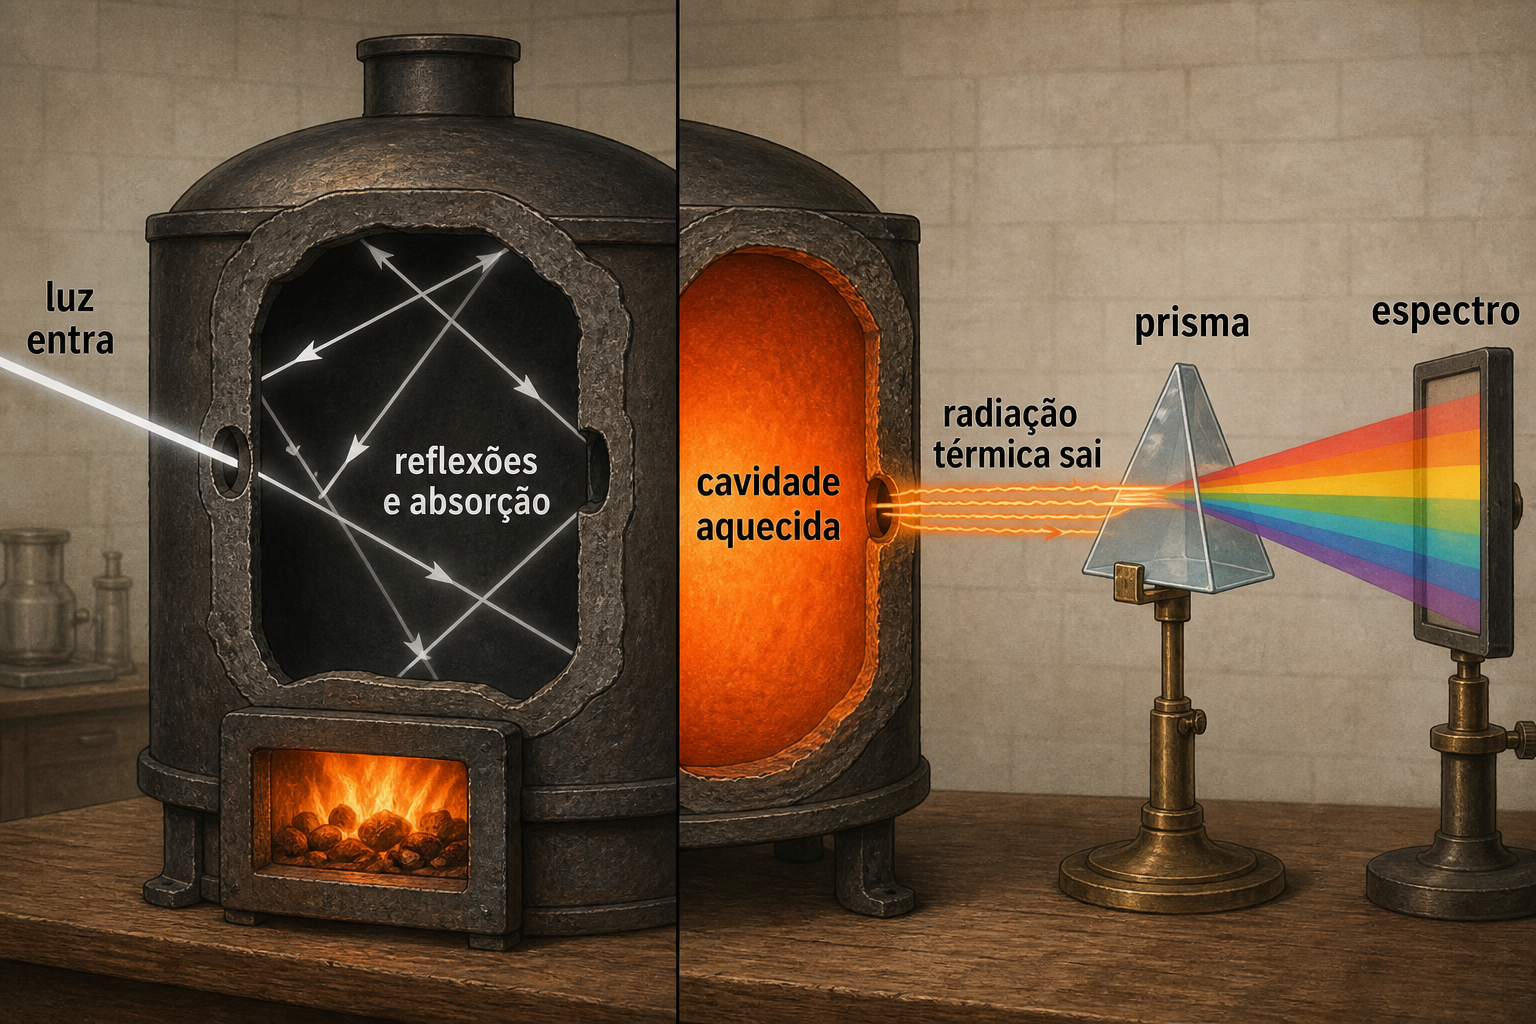
\includegraphics[keepaspectratio]{apostila_files/mediabag/experimento-da-cavid.png}}

}

\caption{Experimento da cavidade}

\end{figure}%

Passando a radiação por um prisma ou uma rede de difração e medindo sua
intensidade, obtemos um espectro contínuo. Todas as faixas são emitidas
simultaneamente; a temperatura muda a intensidade relativa e a posição
do pico.

\href{./assets/simuladores/simulador-corpo-negro.html}{Explorar o
simulador do corpo negro}

\section{Temperatura pelo espectro}\label{temperatura-pelo-espectro}

A lei de Wien relaciona o pico do espectro à temperatura:

\[\lambda_{\max}T=b.\]

O espectro do Sol se aproxima do de um corpo negro a aproximadamente
\(5.800\,\text{K}\).

\begin{figure}[H]

{\centering \pandocbounded{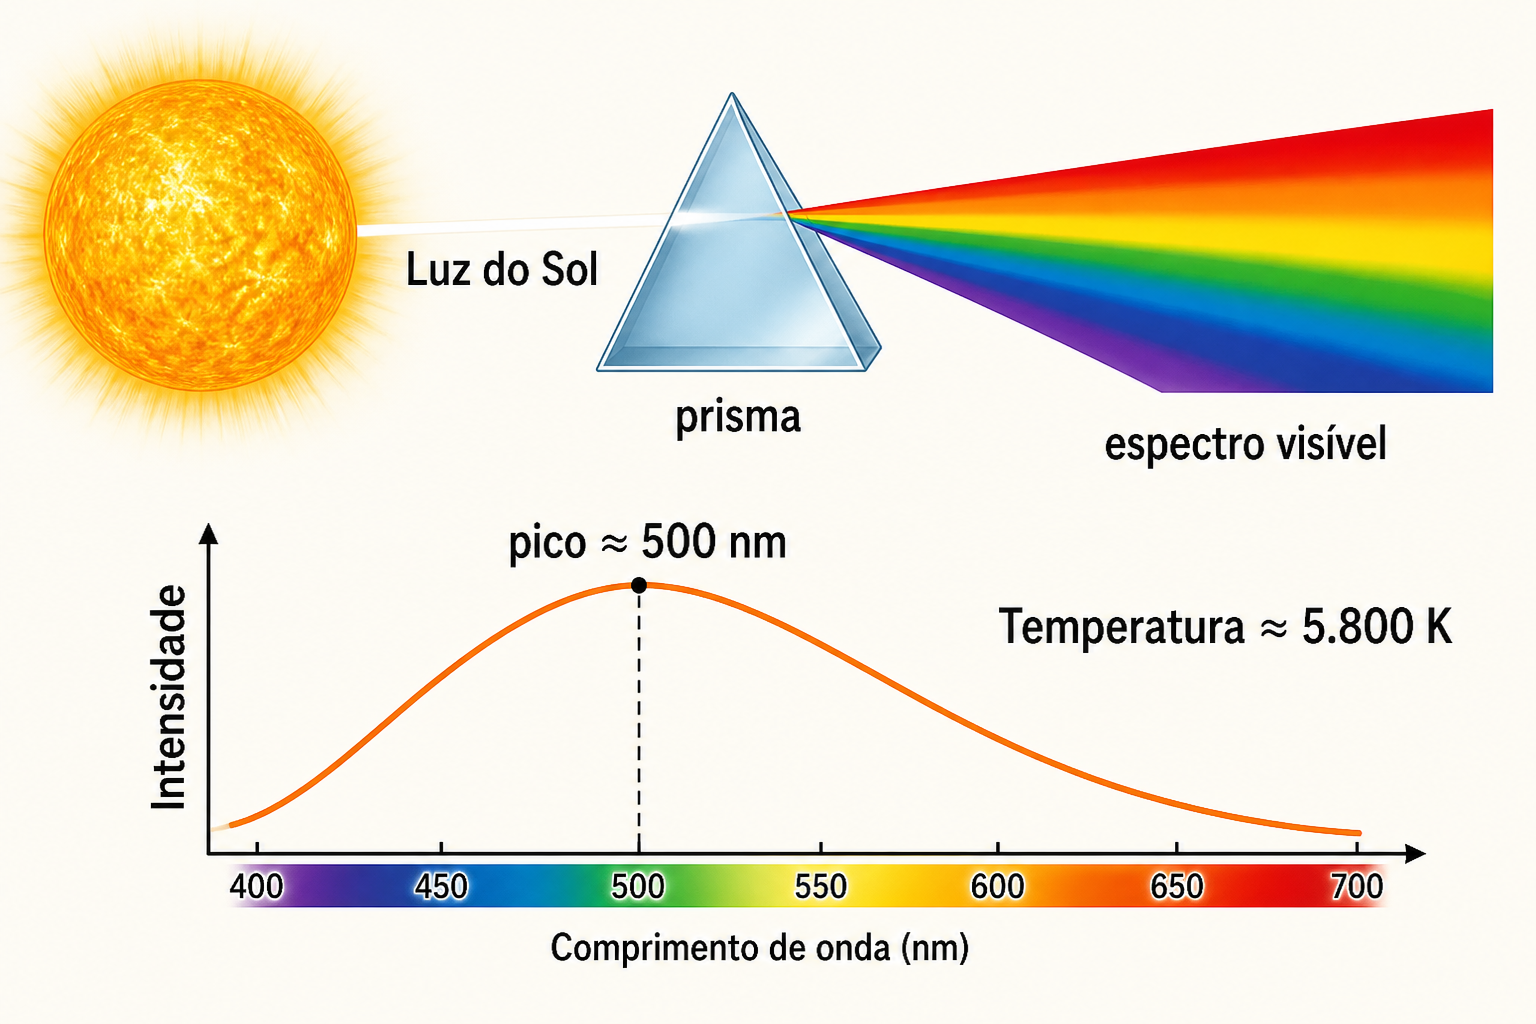
\includegraphics[keepaspectratio]{apostila_files/mediabag/espectro-do-sol-e-te.png}}

}

\caption{Espectro solar e temperatura}

\end{figure}%

\section{A crise clássica}\label{a-crise-cluxe1ssica}

A teoria clássica previa energia ilimitada em frequências altas, a
chamada catástrofe do ultravioleta. Planck resolveu o problema propondo
que os osciladores das paredes trocavam energia em quantidades
discretas:

\[E_n=nhf,\qquad n=0,1,2,\ldots\]

\begin{figure}[H]

{\centering \pandocbounded{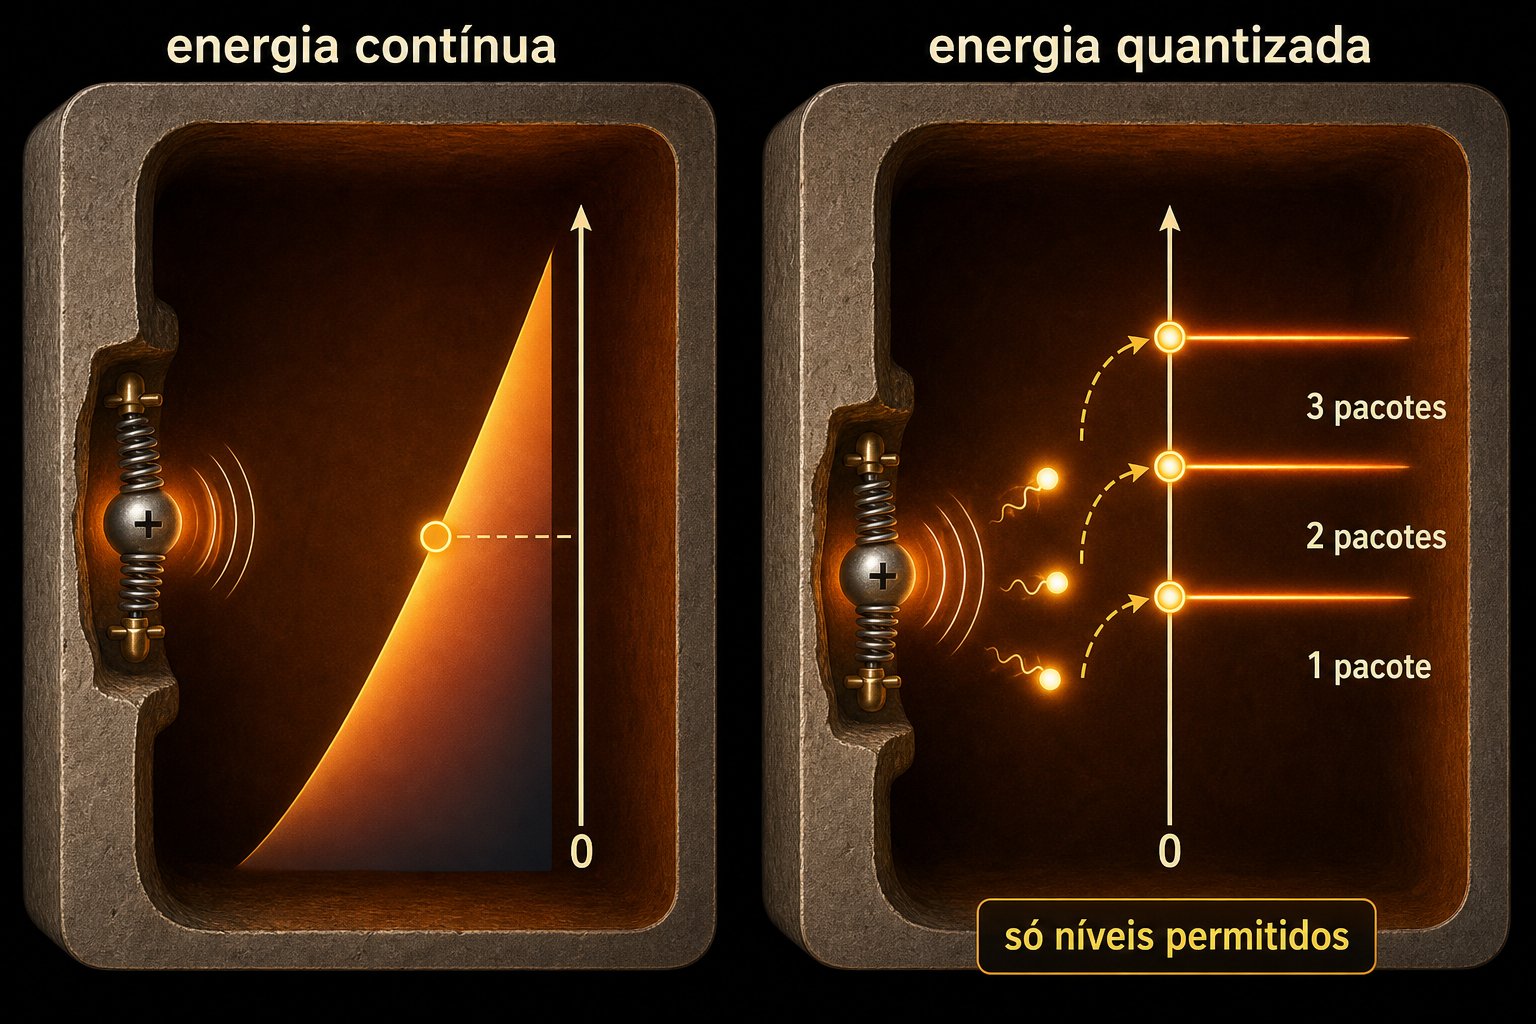
\includegraphics[keepaspectratio]{apostila_files/mediabag/quantizacao-na-cavid.png}}

}

\caption{Quantização na cavidade}

\end{figure}%

\section{Relação com a computação
quântica}\label{relauxe7uxe3o-com-a-computauxe7uxe3o-quuxe2ntica}

Um qubit físico também possui estados de energia controláveis e
transições quantizadas. Em qubits supercondutores, por exemplo, pulsos
de micro-ondas manipulam transições entre dois níveis escolhidos para
representar \(|0\rangle\) e \(|1\rangle\). A constante de Planck e a
relação entre energia e frequência estão no centro desse controle.

\section{Atividade}\label{atividade}

No simulador, aumente a temperatura e registre como variam intensidade,
cor aparente e posição do pico. Explique por que não sai apenas uma cor
pelo furo.

\chapter{Efeito}\label{efeito}

\chapter{Módulo 3 --- Efeito fotoelétrico e
fótons}\label{muxf3dulo-3-efeito-fotoeluxe9trico-e-fuxf3tons}

\section{Experimento}\label{experimento}

Luz incide sobre uma superfície metálica. Quando a frequência é
suficiente, elétrons são ejetados e podem ser coletados por um circuito.
Hallwachs usou uma placa de zinco e luz ultravioleta; outros metais,
como sódio e césio, respondem a frequências menores.

\begin{figure}[H]

{\centering \pandocbounded{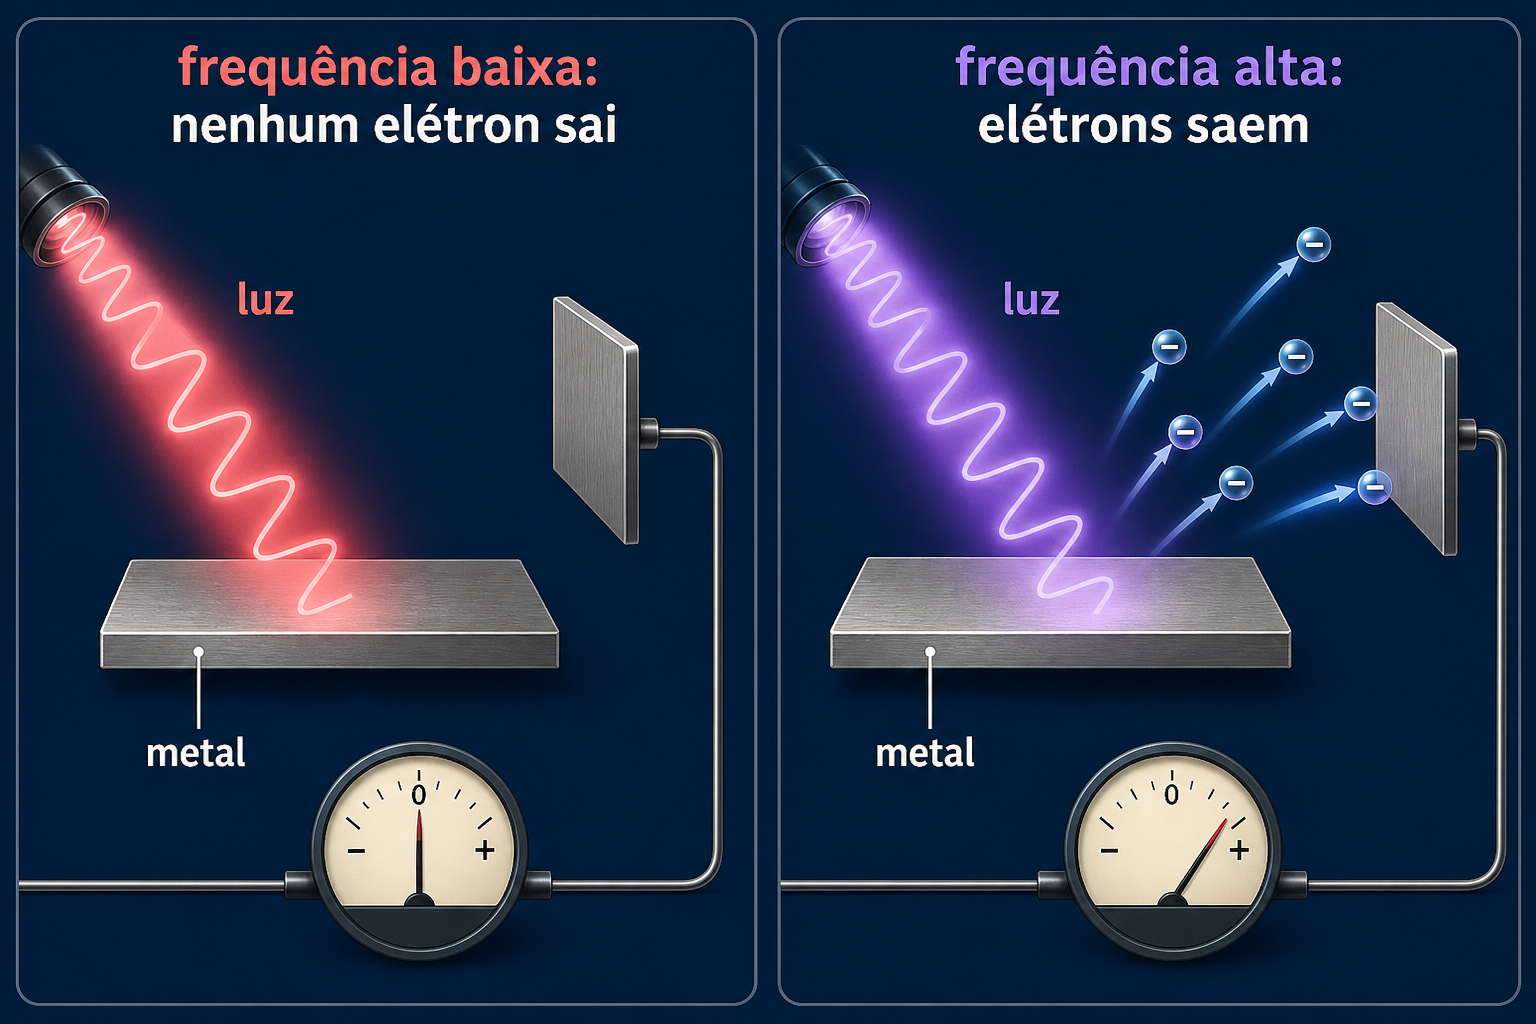
\includegraphics[keepaspectratio]{apostila_files/mediabag/efeito-fotoeletrico.png}}

}

\caption{Efeito fotoelétrico}

\end{figure}%

Os resultados fundamentais são:

\begin{itemize}
\tightlist
\item
  existe uma frequência mínima para cada material;
\item
  abaixo dela, aumentar a intensidade não ejeta elétrons;
\item
  acima dela, maior frequência produz elétrons com maior energia
  cinética;
\item
  maior intensidade significa principalmente mais elétrons emitidos.
\end{itemize}

Einstein explicou o fenômeno atribuindo à luz pacotes de energia:

\[E_{\text{fóton}}=hf,\]

\[K_{\max}=hf-\Phi,\]

onde \(\Phi\) é a energia mínima necessária para liberar o elétron.

\section{Relação com a computação
quântica}\label{relauxe7uxe3o-com-a-computauxe7uxe3o-quuxe2ntica-1}

O experimento mostra que interações quânticas individuais produzem
eventos discretos. Computadores quânticos também terminam em medições
discretas: cada execução devolve bits clássicos, embora o estado
anterior seja descrito por amplitudes. Detectores de fótons e interfaces
luz-matéria também são componentes importantes da computação e
comunicação quânticas fotônicas.

\section{Cuidado conceitual}\label{cuidado-conceitual}

Um elétron não sai necessariamente numa única direção fixa. A direção
depende do material, da luz e das colisões internas; o aparelho coleta
uma distribuição de elétrons.

\chapter{Bohr}\label{bohr}

\chapter{Módulo 4 --- Bohr e níveis de
energia}\label{muxf3dulo-4-bohr-e-nuxedveis-de-energia}

Bohr propôs, em 1913, que o elétron só poderia ocupar determinados
níveis de energia. Uma transição entre níveis envolve emissão ou
absorção de um fóton:

\[hf=|E_f-E_i|.\]

\begin{figure}[H]

{\centering \pandocbounded{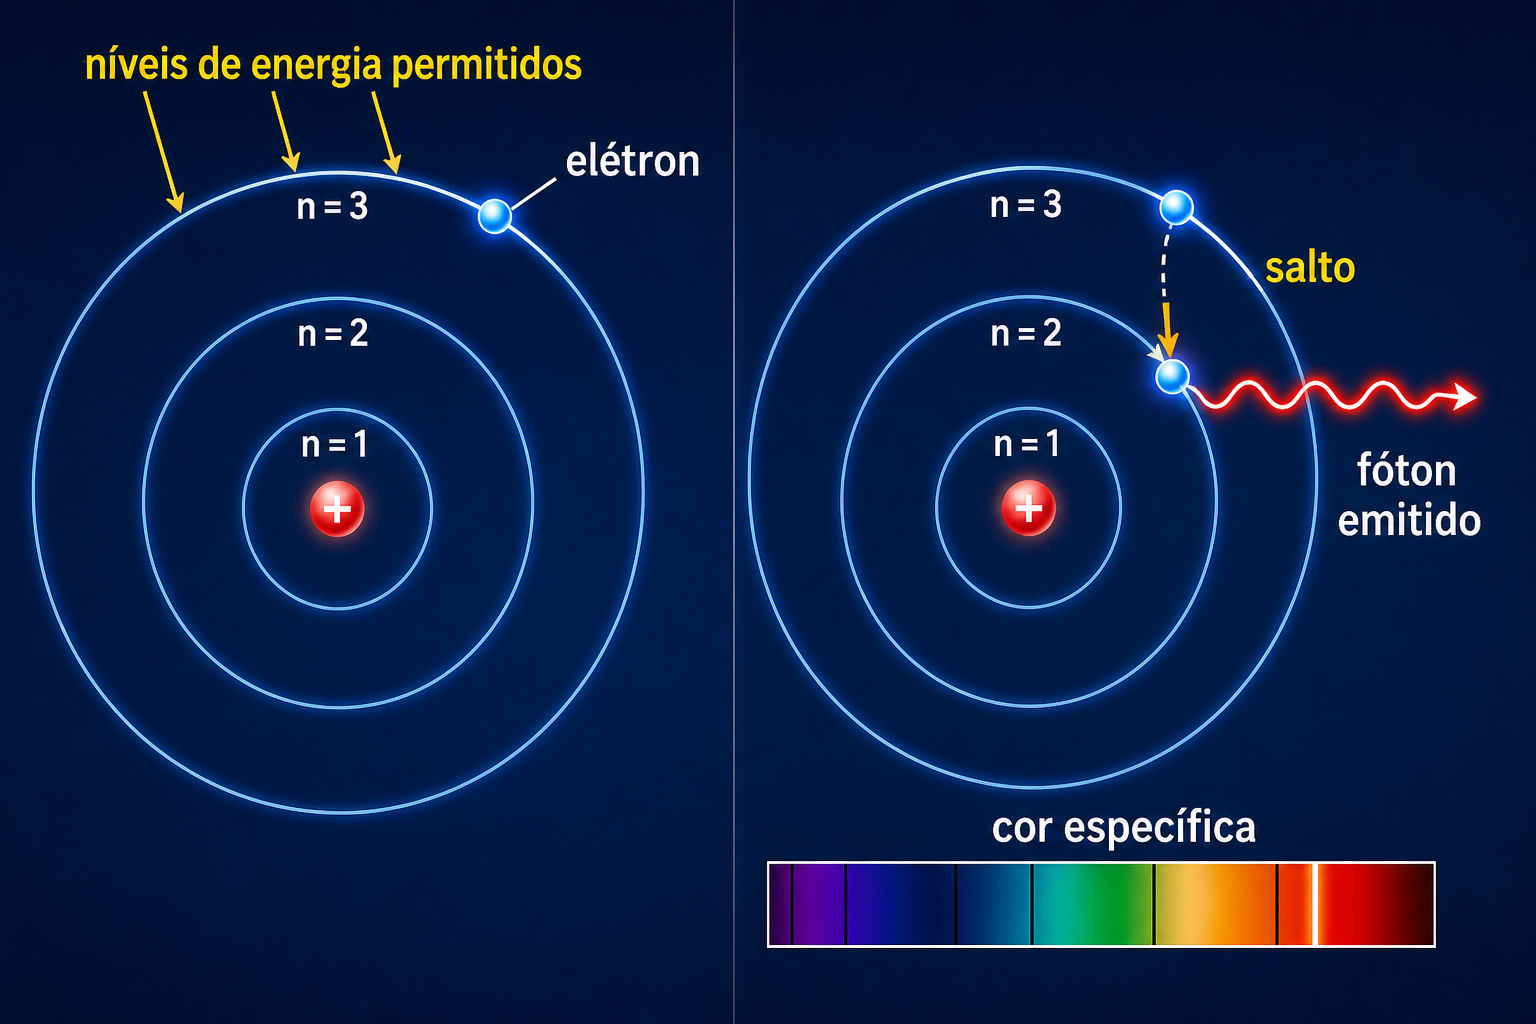
\includegraphics[keepaspectratio]{apostila_files/mediabag/modelo-de-bohr-salto.png}}

}

\caption{Modelo de Bohr}

\end{figure}%

Isso explicou por que átomos emitem linhas espectrais específicas, em
vez de todas as cores possíveis.

\section{Limite do modelo}\label{limite-do-modelo}

A imagem de órbitas circulares é uma etapa histórica, não a descrição
moderna. Na mecânica quântica, elétrons são descritos por estados e
orbitais, não por trajetórias planetárias definidas.

\section{Relação com a computação
quântica}\label{relauxe7uxe3o-com-a-computauxe7uxe3o-quuxe2ntica-2}

Um qubit escolhe dois estados distinguíveis de um sistema quântico e os
chama de \(|0\rangle\) e \(|1\rangle\). Pulsos com frequência ressonante
à diferença de energia permitem controlar transições. O desafio prático
é preservar esses estados contra ruído e evitar transições indesejadas
para outros níveis.

\section{Pergunta de verificação}\label{pergunta-de-verificauxe7uxe3o}

Por que um átomo produz linhas de cores específicas em vez de um
arco-íris contínuo?

\newpage

\chapter{Módulo 3: Ondas de Matéria e Dupla
Fenda}\label{muxf3dulo-3-ondas-de-matuxe9ria-e-dupla-fenda}

\chapter{Aula 03 --- Ondas de Matéria, Função de Onda e Dupla
Fenda}\label{aula-03-ondas-de-matuxe9ria-funuxe7uxe3o-de-onda-e-dupla-fenda}

\chapter{Módulo 5 --- De Broglie e ondas de
matéria}\label{muxf3dulo-5-de-broglie-e-ondas-de-matuxe9ria}

De Broglie propôs que uma partícula com momento \(p\) possui comprimento
de onda:

\[\lambda=\frac{h}{p}.\]

\begin{figure}[H]

{\centering \pandocbounded{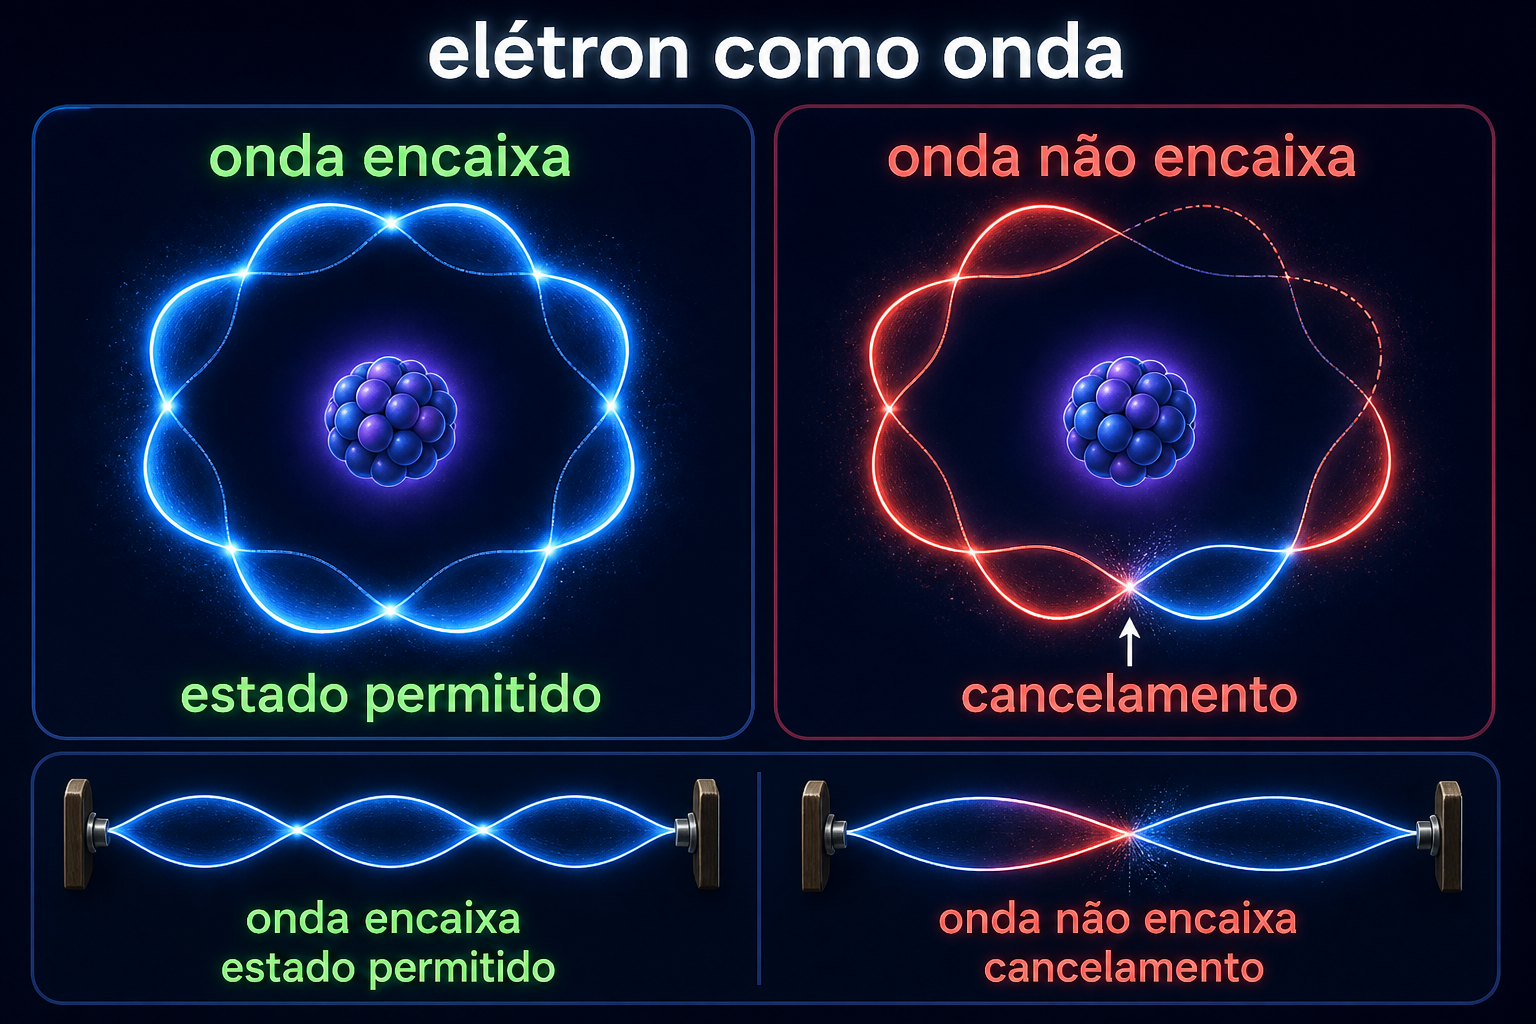
\includegraphics[keepaspectratio]{apostila_files/mediabag/ondas-de-materia-de-.png}}

}

\caption{Ondas de matéria}

\end{figure}%

Padrões ondulatórios permitidos precisam satisfazer condições de
contorno, de modo semelhante a uma onda estacionária numa corda.
Experimentos posteriores de difração de elétrons confirmaram que matéria
pode produzir interferência.

\section{O que é difração?}\label{o-que-uxe9-difrauxe7uxe3o}

É o espalhamento característico de uma onda ao atravessar aberturas ou
contornar estruturas. Regiões de reforço e cancelamento formam um padrão
que partículas clássicas, seguindo apenas trajetórias definidas, não
produziriam.

\section{Relação com a computação
quântica}\label{relauxe7uxe3o-com-a-computauxe7uxe3o-quuxe2ntica-3}

Qubits não são bolinhas clássicas. Seus estados têm amplitudes e fases,
propriedades matemáticas ondulatórias. A computação quântica usa
precisamente a possibilidade de controlar essas fases e fazer amplitudes
interferirem.

\section{Atividade}\label{atividade-1}

Compare uma órbita clássica, uma onda que fecha sobre si mesma e outra
que não fecha. Discuta por que a quantização pode surgir das condições
impostas à onda.

\chapter{Módulo 6 --- Função de onda e dupla
fenda}\label{muxf3dulo-6-funuxe7uxe3o-de-onda-e-dupla-fenda}

\section{Função de onda}\label{funuxe7uxe3o-de-onda}

A função de onda \(\psi\) descreve o estado quântico. Ela não fornece
uma trajetória. O módulo ao quadrado fornece a densidade de
probabilidade:

\[P(x)=|\psi(x)|^2.\]

Cada detecção registra uma partícula inteira em um ponto. Muitas
repetições revelam a distribuição prevista.

\section{Experimento da dupla fenda}\label{experimento-da-dupla-fenda}

Com duas fendas abertas, a amplitude total é:

\[\psi=\psi_1+\psi_2,\]

e a probabilidade é:

\[P=|\psi_1+\psi_2|^2.\]

O termo de interferência cria regiões de reforço e cancelamento. Mesmo
emitindo elétrons um por vez, os pontos acumulados formam franjas.

\href{./assets/simuladores/simulador-fenda-dupla-eletrons-v4.html}{Explorar
o simulador 3D com elétrons}

No simulador:

\begin{itemize}
\tightlist
\item
  o canhão emite elétrons;
\item
  o pacote representa a evolução ondulatória;
\item
  duas amplitudes aparecem depois das fendas;
\item
  cada elétron deixa somente um ponto no anteparo;
\item
  o controle de velocidade muda o ritmo da animação, não a física.
\end{itemize}

\begin{quote}
A animação é um modelo didático. Não representa uma pequena esfera
dividindo-se fisicamente. O que passa a ser combinado são amplitudes
quânticas.
\end{quote}

\section{Relação com a computação
quântica}\label{relauxe7uxe3o-com-a-computauxe7uxe3o-quuxe2ntica-4}

A dupla fenda contém três ingredientes essenciais: superposição de
alternativas, fase relativa e interferência. Um algoritmo quântico
organiza esses mesmos ingredientes no espaço de estados dos qubits.

\section{Experiência complementar: informação de
caminho}\label{experiuxeancia-complementar-informauxe7uxe3o-de-caminho}

Se o aparelho obtém informação capaz de distinguir por qual fenda o
elétron passou, a interferência diminui ou desaparece. Isso introduz
medição, correlação com o ambiente e decoerência --- temas decisivos
para computadores quânticos reais.

\newpage

\chapter{Módulo 4: O Qubit}\label{muxf3dulo-4-o-qubit}

\chapter{Aula 04 --- O Qubit: Fundamentos Matemáticos da Computação
Quântica}\label{aula-04-o-qubit-fundamentos-matemuxe1ticos-da-computauxe7uxe3o-quuxe2ntica}

\chapter{📚 Fundamentos Matemáticos da Computação
Quântica}\label{fundamentos-matemuxe1ticos-da-computauxe7uxe3o-quuxe2ntica}

Bem-vindo! Este notebook foi criado para ajudá-lo a entender os
\textbf{conceitos matemáticos básicos} necessários para trabalhar com
computação quântica.

\section{🎯 O que você vai aprender:}\label{o-que-vocuxea-vai-aprender}

\begin{enumerate}
\def\labelenumi{\arabic{enumi}.}
\tightlist
\item
  \textbf{Estados quânticos} - Como representar qubits matematicamente
\item
  \textbf{Portas quânticas} - Operações que transformam estados
  quânticos
\item
  \textbf{Superposição} - O ``poder'' dos computadores quânticos
\item
  \textbf{Visualizações} - Esfera de Bloch e outras representações
  visuais
\end{enumerate}

\section{💡 Para quem é este
notebook?}\label{para-quem-uxe9-este-notebook}

Se você conhece: - ✅ Álgebra linear básica (vetores e matrizes) - ✅
Números complexos (pelo menos saber que existem 😊) - ✅ Python básico

Então você está pronto para começar! Não se preocupe se alguns conceitos
parecerem estranhos no início - isso é normal em computação quântica.

\textbf{Dica}: Execute cada célula na ordem para acompanhar os exemplos
interativos!

\begin{quote}
Observação Para instalar as bibliotecas abaixo, você deve abrir um
terminal e rodar \texttt{uv\ sync} na raiz deste repositório.
\end{quote}

\begin{Shaded}
\begin{Highlighting}[]
\CommentTok{\# Importando as bibliotecas necessárias}
\CommentTok{\# Não se preocupe se não entender todas agora {-} vamos usá{-}las ao longo do notebook}

\ImportTok{import}\NormalTok{ numpy }\ImportTok{as}\NormalTok{ np                      }\CommentTok{\# Para operações com matrizes e vetores}
\ImportTok{import}\NormalTok{ sympy }\ImportTok{as}\NormalTok{ sp                      }\CommentTok{\# Para matemática simbólica (fórmulas bonitas)}
\ImportTok{from}\NormalTok{ sympy }\ImportTok{import}\NormalTok{ Matrix, symbols       }\CommentTok{\# Para criar matrizes e símbolos matemáticos}
\ImportTok{from}\NormalTok{ IPython.display }\ImportTok{import}\NormalTok{ Markdown    }\CommentTok{\# Para exibir fórmulas formatadas}
\ImportTok{from}\NormalTok{ qiskit.quantum\_info }\ImportTok{import}\NormalTok{ Statevector  }\CommentTok{\# Para trabalhar com estados quânticos}
\ImportTok{from}\NormalTok{ matplotlib }\ImportTok{import}\NormalTok{ pyplot }\ImportTok{as}\NormalTok{ plt    }\CommentTok{\# Para criar gráficos}
\ImportTok{from}\NormalTok{ qiskit.visualization }\ImportTok{import}\NormalTok{ plot\_bloch\_multivector, plot\_state\_qsphere  }\CommentTok{\# Visualizações quânticas}
\end{Highlighting}
\end{Shaded}

\section{🔬 Estados Quânticos
Básicos}\label{estados-quuxe2nticos-buxe1sicos}

Na computação clássica, trabalhamos com \textbf{bits} que podem ser 0 ou
1.

Na computação quântica, trabalhamos com \textbf{qubits} que podem estar
em: - \textbf{Estado \textbar0⟩} (lê-se ``ket zero'') - equivalente ao
bit clássico 0 - \textbf{Estado \textbar1⟩} (lê-se ``ket um'') -
equivalente ao bit clássico 1 - \textbf{Superposição de \textbar0⟩ e
\textbar1⟩} - aqui está a mágica! O qubit pode estar em ``ambos''
estados simultaneamente

\subsection{📌 Notação matemática:}\label{notauxe7uxe3o-matemuxe1tica}

Representamos esses estados como \textbf{vetores coluna} em ``ket psi''.
Em geral:

\(|\psi⟩ = \begin{bmatrix} \text{amplitude para estado } \alpha  \\ \text{amplitude para estado } \beta \end{bmatrix}\)

Essa amplitude pode variar de \(-1\) a \(1\) em números reais ou é um
número complexo cujo módulo (valor absoluto) é menor ou igual a 1.

Assim:

\begin{itemize}
\tightlist
\item
  Estado \textbar0⟩ = \(\begin{bmatrix} 1 \\ 0 \end{bmatrix}\)

  \begin{itemize}
  \tightlist
  \item
    \textbf{Primeira posição (1)}: Amplitude para o estado \textbar0⟩
  \item
    \textbf{Segunda posição (0)}: Amplitude para o estado \textbar1⟩
  \item
    ➡️ Interpretação: 100\% de probabilidade de medir 0, 0\% de
    probabilidade de medir 1
  \end{itemize}
\item
  Estado \textbar1⟩ = \(\begin{bmatrix} 0 \\ 1 \end{bmatrix}\)

  \begin{itemize}
  \tightlist
  \item
    \textbf{Primeira posição (0)}: Amplitude para o estado \textbar0⟩
  \item
    \textbf{Segunda posição (1)}: Amplitude para o estado \textbar1⟩
  \item
    ➡️ Interpretação: 0\% de probabilidade de medir 0, 100\% de
    probabilidade de medir 1
  \end{itemize}
\end{itemize}

\textbf{Regra geral}: Para qualquer qubit
\(|\psi⟩ = \begin{bmatrix} \alpha \\ \beta \end{bmatrix}\): - O valor
\textbf{\(\alpha\)} (primeira linha) representa a amplitude do estado
\textbar0⟩ - O valor \textbf{\(\beta\)} (segunda linha) representa a
amplitude do estado \textbar1⟩ - As probabilidades são: P(0) =
\textbar{}\(\alpha\)\textbar² e P(1) = \textbar{}\(\beta\)\textbar² -
Sempre vale: \textbar{}\(\alpha\)\textbar² +
\textbar{}\(\beta\)\textbar² = 1 (normalização)

\textbf{Por que vetores?} Porque podemos aplicar transformações
matemáticas (matrizes) neles, e isso é exatamente o que as portas
quânticas naturalmente fazem!

\begin{Shaded}
\begin{Highlighting}[]
\CommentTok{\# Vamos criar esses estados básicos usando SymPy (biblioteca de matemática simbólica)}
\CommentTok{\# Isso nos permite trabalhar com fórmulas matemáticas de forma elegante}

\CommentTok{\# Estado |0⟩ {-} primeiro número é 1, segundo é 0}
\NormalTok{ket\_0 }\OperatorTok{=}\NormalTok{ Matrix([[}\DecValTok{1}\NormalTok{], }
\NormalTok{                [}\DecValTok{0}\NormalTok{]])}

\CommentTok{\# Estado |1⟩ {-} primeiro número é 0, segundo é 1}
\NormalTok{ket\_1 }\OperatorTok{=}\NormalTok{ Matrix([[}\DecValTok{0}\NormalTok{], }
\NormalTok{                [}\DecValTok{1}\NormalTok{]])}

\CommentTok{\# Exibir de forma bonita com LaTeX (notação matemática profissional)}
\NormalTok{display(Markdown(}\SpecialStringTok{f"$$}\CharTok{\textbackslash{}\textbackslash{}}\SpecialStringTok{ket}\CharTok{\{\{}\SpecialStringTok{0}\CharTok{\}\}}\SpecialStringTok{ = }\SpecialCharTok{\{}\NormalTok{sp}\SpecialCharTok{.}\NormalTok{latex(ket\_0)}\SpecialCharTok{\}}\SpecialStringTok{$$"}\NormalTok{))}
\NormalTok{display(Markdown(}\SpecialStringTok{f"$$}\CharTok{\textbackslash{}\textbackslash{}}\SpecialStringTok{ket}\CharTok{\{\{}\SpecialStringTok{1}\CharTok{\}\}}\SpecialStringTok{ = }\SpecialCharTok{\{}\NormalTok{sp}\SpecialCharTok{.}\NormalTok{latex(ket\_1)}\SpecialCharTok{\}}\SpecialStringTok{$$"}\NormalTok{))}

\BuiltInTok{print}\NormalTok{(}\StringTok{"}\CharTok{\textbackslash{}n}\StringTok{✅ Estados básicos criados com sucesso!"}\NormalTok{)}
\end{Highlighting}
\end{Shaded}

\[\ket{0} = \left[\begin{matrix}1\\0\end{matrix}\right]\]

\[\ket{1} = \left[\begin{matrix}0\\1\end{matrix}\right]\]

\begin{verbatim}

✅ Estados básicos criados com sucesso!
\end{verbatim}

\begin{verbatim}

✅ Estados básicos criados com sucesso!
\end{verbatim}

\begin{Shaded}
\begin{Highlighting}[]
\CommentTok{\# Agora vamos criar os MESMOS estados usando NumPy (só para fins de comparação de bibliotecas)}
\CommentTok{\# NumPy é mais eficiente para cálculos numéricos (com números reais)}

\CommentTok{\# Estado |0⟩ usando NumPy}
\NormalTok{q\_zero }\OperatorTok{=}\NormalTok{ np.array([}
\NormalTok{    [}\DecValTok{1}\NormalTok{],   }\CommentTok{\# Probabilidade 100\% de medir 0}
\NormalTok{    [}\DecValTok{0}\NormalTok{]    }\CommentTok{\# Probabilidade 0\% de medir 1}
\NormalTok{])}

\CommentTok{\# Estado |1⟩ usando NumPy}
\NormalTok{q\_one }\OperatorTok{=}\NormalTok{ np.array([}
\NormalTok{    [}\DecValTok{0}\NormalTok{],   }\CommentTok{\# Probabilidade 0\% de medir 0}
\NormalTok{    [}\DecValTok{1}\NormalTok{]    }\CommentTok{\# Probabilidade 100\% de medir 1}
\NormalTok{])}

\BuiltInTok{print}\NormalTok{(}\StringTok{"=== Estado |0⟩ ==="}\NormalTok{)}
\BuiltInTok{print}\NormalTok{(q\_zero)}
\BuiltInTok{print}\NormalTok{(}\StringTok{"}\CharTok{\textbackslash{}n}\StringTok{=== Estado |1⟩ ==="}\NormalTok{)}
\BuiltInTok{print}\NormalTok{(q\_one)}

\BuiltInTok{print}\NormalTok{(}\StringTok{"}\CharTok{\textbackslash{}n}\StringTok{💡 Dica: Esses vetores representam a \textquotesingle{}probabilidade\textquotesingle{} de medir cada resultado!"}\NormalTok{)}
\end{Highlighting}
\end{Shaded}

\begin{verbatim}
=== Estado |0⟩ ===
[[1]
 [0]]

=== Estado |1⟩ ===
[[0]
 [1]]

💡 Dica: Esses vetores representam a 'probabilidade' de medir cada resultado!
\end{verbatim}

\begin{verbatim}
=== Estado |0⟩ ===
[[1]
 [0]]

=== Estado |1⟩ ===
[[0]
 [1]]

💡 Dica: Esses vetores representam a 'probabilidade' de medir cada resultado!
\end{verbatim}

\section{🌟 Superposição: o coração da Computação
Quântica}\label{superposiuxe7uxe3o-o-corauxe7uxe3o-da-computauxe7uxe3o-quuxe2ntica}

Aqui está onde a mágica acontece! Um qubit pode estar em uma
\textbf{combinação} dos estados \textbar0⟩ e \textbar1⟩:

\[|ψ⟩ = 𝛼|0⟩ + 𝛽|1⟩\]

Onde: - \textbf{\textbar ψ⟩} (lê-se ``ket psi'') é o estado do qubit -
\textbf{𝛼} (alpha) e \textbf{𝛽} (beta) são \textbf{números complexos}
chamados de \textbf{amplitudes} - \textbf{Regra de ouro}:
\(|𝛼|² + |𝛽|²= 1\) (aqui também essas probabilidades precisam somar
100\%!)

\subsection{🎲 Como interpretar as
amplitudes:}\label{como-interpretar-as-amplitudes}

\begin{itemize}
\tightlist
\item
  \(|𝛼|²\) = probabilidade de medir \textbf{0}
\item
  \(|𝛽|²\) = probabilidade de medir \textbf{1}
\end{itemize}

\subsection{📊 Exemplo visual:}\label{exemplo-visual}

Se \(𝛼 = \frac{1}{\sqrt{2}}\) e \(𝛽 = \frac{1}{\sqrt{2}}\)?

``Montando'' a combinação dos estados \textbar0⟩ e \textbar1⟩, ficará
assim:

\[|ψ⟩ = \frac{1}{\sqrt{2}}|0⟩ + \frac{1}{\sqrt{2}}|1⟩\]

Se quiser, pra ficar mais claro, podemos substituir os kets pelos seus
vetores, até para ficar mais intuitivo e você sempre imaginar que por
trás desses kets, existem, na verdade, vetores:

\[|ψ⟩ = \frac{1}{\sqrt{2}} \begin{bmatrix} 1 \\ 0 \end{bmatrix} + \frac{1}{\sqrt{2}} \begin{bmatrix} 0 \\ 1 \end{bmatrix}\]

Assim, não precisamos sempre usar vetores, mas é bom saber que eles
estão lá por trás.

Agora, calculando as probabilidades:

\begin{itemize}
\tightlist
\item
  Probabilidade de medir 0:
  \(\left(\frac{1}{\sqrt{2}}\right)² = \frac{1}{2} = 0.50 = 50\%\)
\item
  Probabilidade de medir 1:
  \(\left(\frac{1}{\sqrt{2}}\right)² = \frac{1}{2} = 0.50 = 50\%\)
\end{itemize}

\textbf{Em vetores:}

\[|ψ⟩ = 𝛼 \begin{bmatrix} 1 \\ 0 \end{bmatrix} + 𝛽 \begin{bmatrix} 0 \\ 1 \end{bmatrix} = \begin{bmatrix} 𝛼 \\ 𝛽 \end{bmatrix}\]

\[|ψ⟩ = 𝛼|0⟩ + 𝛽|1⟩\]

Simples assim! O primeiro número é a amplitude para \textbar0⟩, o
segundo para \textbar1⟩.

\begin{Shaded}
\begin{Highlighting}[]
\CommentTok{\# Vamos criar um estado genérico em superposição!}
\CommentTok{\# Usamos símbolos 𝛼 (alpha) e 𝛽 (beta) para representar valores desconhecidos}

\NormalTok{alpha, beta }\OperatorTok{=}\NormalTok{ symbols(}\StringTok{\textquotesingle{}alpha beta\textquotesingle{}}\NormalTok{, }\BuiltInTok{complex}\OperatorTok{=}\VariableTok{True}\NormalTok{)   }\CommentTok{\# Definindo 𝛼 e 𝛽 como números complexos}
\NormalTok{psi }\OperatorTok{=}\NormalTok{ alpha }\OperatorTok{*}\NormalTok{ ket\_0 }\OperatorTok{+}\NormalTok{ beta }\OperatorTok{*}\NormalTok{ ket\_1                  }\CommentTok{\# Estado genérico em superposição}

\BuiltInTok{print}\NormalTok{(}\StringTok{"Estado quântico genérico criado:"}\NormalTok{)}

\NormalTok{display(Markdown(}\SpecialStringTok{f"$$}\CharTok{\textbackslash{}\textbackslash{}}\SpecialStringTok{ket}\CharTok{\{\{\textbackslash{}\textbackslash{}}\SpecialStringTok{psi}\CharTok{\}\}}\SpecialStringTok{ = }\SpecialCharTok{\{}\NormalTok{sp}\SpecialCharTok{.}\NormalTok{latex(psi)}\SpecialCharTok{\}}\SpecialStringTok{$$"}\NormalTok{))}

\BuiltInTok{print}\NormalTok{(}\StringTok{"}\CharTok{\textbackslash{}n}\StringTok{💡 Isso significa:"}\NormalTok{)}
\BuiltInTok{print}\NormalTok{(}\StringTok{"   {-} Com probabilidade |α|², medimos 0"}\NormalTok{)}
\BuiltInTok{print}\NormalTok{(}\StringTok{"   {-} Com probabilidade |β|², medimos 1"}\NormalTok{)}
\BuiltInTok{print}\NormalTok{(}\StringTok{"   {-} Antes da medição, o qubit está em AMBOS os estados!"}\NormalTok{)}
\end{Highlighting}
\end{Shaded}

\begin{verbatim}
Estado quântico genérico criado:
\end{verbatim}

\[\ket{\psi} = \left[\begin{matrix}\alpha\\\beta\end{matrix}\right]\]

\begin{verbatim}

💡 Isso significa:
   - Com probabilidade |α|², medimos 0
   - Com probabilidade |β|², medimos 1
   - Antes da medição, o qubit está em AMBOS os estados!
\end{verbatim}

\begin{verbatim}
Estado quântico genérico criado:
\end{verbatim}

\begin{verbatim}

💡 Isso significa:
   - Com probabilidade |α|², medimos 0
   - Com probabilidade |β|², medimos 1
   - Antes da medição, o qubit está em AMBOS os estados!
\end{verbatim}

\section{🌀 E o que é esse termo
``superposição''?}\label{e-o-que-uxe9-esse-termo-superposiuxe7uxe3o}

Superposição é o fenômeno quântico onde um qubit pode existir em
múltiplos estados ao mesmo tempo. Diferente dos bits clássicos que são
ou 0 ou 1, um qubit em superposição pode ser uma combinação de ambos os
estados.

\begin{quote}
\emph{Como assim? Eu estou acostumado a pensar que algo é 0 ou 1, não
ambos ao mesmo tempo!} 🤔
\end{quote}

Imagine uma moeda girando no ar 🪙 (esse é um comparativo clássico da
literatura!). Enquanto está girando, ela não é nem cara nem coroa - está
em um estado de superposição de ambos os lados. Só quando a moeda cai e
você olha para ela 👀 é que ela ``decide'' ser cara ou coroa. Então,
olhar para a moeda é como medir um qubit: você força ele a escolher um
estado específico (0 ou 1), fazendo-o parar de girar.

Obviamente, se você for teimoso, vai dizer que os dois não são cara e
coroa ao mesmo tempo, pois se você usar uma supercâmera de altíssima
velocidade 📹, verá que a moeda está em um estado definido a cada
instante. Em câmera super lenta, você verá que a moeda ou está em cara,
ou em coroa. OK, teimoso, você está certo! Porém, entretanto,
todavia\ldots{}

No mundo quântico ⚛️, se essa moeda existisse - vamos chamar de moeda
quântica 🪙✨ - ele seria cara e coroa ao mesmo tempo. Somente quando
você a observasse é que poderia saber se é cara ou coroa. Na
visualização, o movimento de giro é destruído ao ser observado. A moeda
cai e para. Você perdeu a informação do movimento (superposição) e ficou
apenas com o resultado estático (0 ou 1), e só a partir daí você sabe o
resultado final. Estranho não é? Bem-vindo ao mundo quântico! 🎭

\begin{quote}
⚡ O que acontece: O qubit (o objeto físico, como um elétron ou átomo)
geralmente não é destruído (a menos que seja um fóton sendo absorvido
por um detector). O que é ``destruído'' irremediavelmente é a informação
da superposição (a parte quântica, o giro). O qubit continua lá, mas
agora ele é apenas um bit clássico chato (está parado em cara ou coroa)
\end{quote}

Entender isso (e aceitar) é crucial para compreender como os
computadores quânticos funcionam e por que eles são tão poderosos para
certas tarefas. Daqui para frente, sempre que falarmos de qubits em
superposição, lembre-se da moeda quântica girando no ar!

Em \url{03-mais-sobre-Hadamard.md} existe um experimento físico feito
com fótons 💡 que ilustra muito bem esse conceito de superposição e
medição quântica. Recomendo fortemente a leitura para aprofundar sua
compreensão, caso estejas curioso! Somente me convenci intuitivamente
disso após ler aquele experimento.

\begin{quote}
📊 O que acontece: quando aplicamos uma porta Hadamard (veremos depois)
e colocamos o qubit em um estado de superposição (como o estado
\(|+\rangle\)), ele passa a ter 50\% de chance de ser medido como 0 e
50\% de chance de ser medido como 1. Ao fazer a medição, ele `colapsa'
(faz parar) essa superposição em um dos estados possíveis.''
\end{quote}

Daí sempre precisamos realizar múltiplas medições para termos uma boa
ideia das probabilidades reais envolvidas. É como jogar a moeda quântica
1024 vezes 🎲 - chamamos de 1024 shots - para ver quantas vezes ela cai
em cara ou coroa! Uma hora pode ser 30\% de cara, outra hora 70\%. Em
outro momento pode ser 33\% de cara. Mas se você jogar 1024 vezes, verá
que a média se aproxima dos 50\% esperados. Você consegue entender que o
fim do cálculo se baseia, na verdade, em probabilidades estatísticas,
certo? Não é como somar 1 + 1 = 2, onde o resultado é sempre o mesmo.
Aqui, o resultado pode variar a cada experimento, mas a média de muitos
experimentos converge para o valor esperado.

\begin{quote}
📈 Observação: É padrão realizar, por exemplo, 1024 shots para construir
um histograma de probabilidades e ver qual é a resposta mais provável.
\end{quote}

Claro que em um computador clássico 💻 fazer cálculo (1 + 1 = 2) de
forma quântica demoraria muito, e seria coisa de louco calcular
probabilidades estatísticas para tudo. Porém, você vai ver mais a
frente, que existem certos cálculos que um computador clássico não
consegue fazer de forma eficiente, pois se conseguisse, não haveria
necessidade de um outro tipo de computador, certo? E é aí que entra o
computador quântico 🖥️⚛️. Ele não precisa `calcular' essas
probabilidades uma a uma; ele manipula as ondas de probabilidade
(amplitudes) usando superposição, entrelaçamento e interferência para
que, no final, a resposta correta tenha a maior chance de ser medida.
Mas isso é assunto para os próximos notebooks!

\begin{quote}
💾 O que acontece: É explicado que para simular um sistema quântico de
\(n\) qubits, um computador clássico precisa armazenar \(2^n\) números
complexos (as amplitudes). Isso cresce exponencialmente. Com apenas 64
qubits, seriam necessários cerca de 18 quintilhões de números complexos,
o que excede a capacidade de armazenamento atual para um computador
clássico (este sofre para calcular essas amplitudes)!
\end{quote}

Assim, quando você ouvir dizer que os cálculos realizados em um
computador clássico são determinísticos (a gente sabe onde vai dar o
resultado se fizermos ``na mão''), enquanto os cálculos em um computador
quântico são probabilísticos (é provável que dê 50\% para\ldots), agora
você entenderá o porquê!

\textbf{✨ A superposição não é ser A e B. É ter a potencialidade de ser
A ou B, com uma probabilidade que nós podemos controlar.}

\section{⚙️ Portas Quânticas: Transformando
Estados}\label{portas-quuxe2nticas-transformando-estados}

Portas quânticas são \textbf{transformações} que aplicamos aos qubits.
Matematicamente, são \textbf{matrizes} que multiplicamos pelos vetores
de estado.

Da mesma forma que em computação clássica temos portas lógicas (AND, OR,
NOT) que manipulam bits, em computação quântica temos portas quânticas
que manipulam qubits.

\textbf{Analogia:} Se um estado quântico é como uma formiga em cima de
uma bola (Esfera de Bloch), uma porta quântica é como uma rotação que
move a formiga para uma nova posição na bola.

\subsection{🔄 Principais Portas
Quânticas:}\label{principais-portas-quuxe2nticas}

\begin{enumerate}
\def\labelenumi{\arabic{enumi}.}
\tightlist
\item
  \textbf{Porta X (NOT quântico)} - Inverte \textbar0⟩ ↔ \textbar1⟩
  (como o NOT da computação clássica)
\item
  \textbf{Porta H (Hadamard)} - Cria superposição (a porta mais
  importante!)
\item
  \textbf{Portas de Fase (Z, S, T)} - Modificam a fase sem mudar
  probabilidades
\end{enumerate}

Vamos explorar cada uma delas!

\begin{quote}
⚠️ \textbf{Importante}: Vamos trabalhar com kets ao representar os
estados quânticos, como \textbar0⟩ e \textbar1⟩, para manter a notação
padrão da computação quântica. Lembre-se que por trás desses kets,
existem vetores coluna que representam os estados matematicamente, só
isso!
\end{quote}

\subsection{🚪 Porta X (NOT Quântico)}\label{porta-x-not-quuxe2ntico}

É a versão quântica do NOT clássico. Funciona assim: - Se o qubit está
em \textbar0⟩ → vira \textbar1⟩ - Se o qubit está em \textbar1⟩ → vira
\textbar0⟩

Se fossemos usar vetores, seria: - Se o qubit está em
\(\begin{bmatrix} 1 \\ 0 \end{bmatrix}\) → vira
\(\begin{bmatrix} 0 \\ 1 \end{bmatrix}\) - Se o qubit está em
\(\begin{bmatrix} 0 \\ 1 \end{bmatrix}\) → vira
\(\begin{bmatrix} 1 \\ 0 \end{bmatrix}\)

\textbf{Matriz da Porta X:}

\[X = \begin{bmatrix} 0 & 1 \\ 1 & 0 \end{bmatrix}\]

\textbf{Como funciona:}

A função é simbolizada como X\textbar ψ⟩, onde \textbar ψ⟩ é o estado do
qubit. Assim, é como se:

\begin{itemize}
\tightlist
\item
  em \(X\) você substitui o \(X\) pela matriz da porta X que é
  \(\begin{bmatrix} 0 & 1 \\ 1 & 0 \end{bmatrix}\)
\item
  e o \(|0⟩\) pelo vetor correspondente a \textbar0⟩, que é
  \(\begin{bmatrix} 1 \\ 0 \end{bmatrix}\).
\end{itemize}

Então, juntando \(X\) e \(|0⟩\), temos \(X|0⟩\):

\[X|0⟩ = \begin{bmatrix} 0 & 1 \\ 1 & 0 \end{bmatrix} \begin{bmatrix} 1 \\ 0 \end{bmatrix}\]

Daqui é só continuar com o cálculo sobre a multiplicação de matrizes
para ver o resultado final:

\[\begin{bmatrix} 0 & 1 \\ 1 & 0 \end{bmatrix} \begin{bmatrix} 1 \\ 0 \end{bmatrix} = \begin{bmatrix} 0 \\ 1 \end{bmatrix}\]

E você percebe com que \(\begin{bmatrix} 0 \\ 1 \end{bmatrix}\) se
parece? Sim! É o vetor correspondente a \textbar1⟩. Então, concluímos
que:

\[X|0⟩ = \begin{bmatrix} 0 & 1 \\ 1 & 0 \end{bmatrix} \begin{bmatrix} 1 \\ 0 \end{bmatrix} = \begin{bmatrix} 0 \\ 1 \end{bmatrix} = |1⟩\]

E para \(X|1⟩\)?

\[X|1⟩ = \begin{bmatrix} 0 & 1 \\ 1 & 0 \end{bmatrix} \begin{bmatrix} 0 \\ 1 \end{bmatrix} = \begin{bmatrix} 1 \\ 0 \end{bmatrix} = |0⟩\]

\textbf{Dica:} Multiplicação de matrizes é só ``linha × coluna e
somar''!

\begin{Shaded}
\begin{Highlighting}[]
\CommentTok{\# Vamos testar a porta X na prática com Python!}

\CommentTok{\# Definir a matriz da porta X}
\NormalTok{X }\OperatorTok{=}\NormalTok{ Matrix([[}\DecValTok{0}\NormalTok{, }\DecValTok{1}\NormalTok{],}
\NormalTok{            [}\DecValTok{1}\NormalTok{, }\DecValTok{0}\NormalTok{]])}

\BuiltInTok{print}\NormalTok{(}\StringTok{"🔄 Aplicando a Porta X...}\CharTok{\textbackslash{}n}\StringTok{"}\NormalTok{)}

\CommentTok{\# Aplicar X ao estado |0⟩}
\NormalTok{result\_0 }\OperatorTok{=}\NormalTok{ X }\OperatorTok{*}\NormalTok{ ket\_0        }\CommentTok{\# ket\_0 é o estado |0⟩ com o vetor definido no código lá atrás, lembra?}
\BuiltInTok{print}\NormalTok{(}\StringTok{"Teste 1: X|0⟩ deve dar |1⟩"}\NormalTok{)}
\NormalTok{display(Markdown(}\SpecialStringTok{f"$$X }\CharTok{\textbackslash{}\textbackslash{}}\SpecialStringTok{ket}\CharTok{\{\{}\SpecialStringTok{0}\CharTok{\}\}}\SpecialStringTok{ = }\SpecialCharTok{\{}\NormalTok{sp}\SpecialCharTok{.}\NormalTok{latex(result\_0)}\SpecialCharTok{\}}\SpecialStringTok{$$ ✅"}\NormalTok{))}

\CommentTok{\# Aplicar X ao estado |1⟩}
\NormalTok{result\_1 }\OperatorTok{=}\NormalTok{ X }\OperatorTok{*}\NormalTok{ ket\_1}
\BuiltInTok{print}\NormalTok{(}\StringTok{"}\CharTok{\textbackslash{}n}\StringTok{Teste 2: X|1⟩ deve dar |0⟩"}\NormalTok{)}
\NormalTok{display(Markdown(}\SpecialStringTok{f"$$X }\CharTok{\textbackslash{}\textbackslash{}}\SpecialStringTok{ket}\CharTok{\{\{}\SpecialStringTok{1}\CharTok{\}\}}\SpecialStringTok{ = }\SpecialCharTok{\{}\NormalTok{sp}\SpecialCharTok{.}\NormalTok{latex(result\_1)}\SpecialCharTok{\}}\SpecialStringTok{$$ ✅"}\NormalTok{))}

\BuiltInTok{print}\NormalTok{(}\StringTok{"}\CharTok{\textbackslash{}n}\StringTok{💡 A porta X realmente inverte os estados, como esperado!"}\NormalTok{)}
\end{Highlighting}
\end{Shaded}

\begin{verbatim}
🔄 Aplicando a Porta X...

Teste 1: X|0⟩ deve dar |1⟩
\end{verbatim}

\[X \ket{0} = \left[\begin{matrix}0\\1\end{matrix}\right]\] ✅

\begin{verbatim}

Teste 2: X|1⟩ deve dar |0⟩
\end{verbatim}

\[X \ket{1} = \left[\begin{matrix}1\\0\end{matrix}\right]\] ✅

\begin{verbatim}

💡 A porta X realmente inverte os estados, como esperado!
\end{verbatim}

\begin{verbatim}
🔄 Aplicando a Porta X...

Teste 1: X|0⟩ deve dar |1⟩
\end{verbatim}

\begin{verbatim}

Teste 2: X|1⟩ deve dar |0⟩
\end{verbatim}

\begin{verbatim}

💡 A porta X realmente inverte os estados, como esperado!
\end{verbatim}

\begin{Shaded}
\begin{Highlighting}[]
\CommentTok{\# Agora vamos definir a porta X usando NumPy (outra maneira de fazer a mesma coisa)}

\NormalTok{gate\_x }\OperatorTok{=}\NormalTok{ np.array([}
\NormalTok{    [}\DecValTok{0}\NormalTok{, }\DecValTok{1}\NormalTok{],  }\CommentTok{\# Primeira linha da matriz}
\NormalTok{    [}\DecValTok{1}\NormalTok{, }\DecValTok{0}\NormalTok{]   }\CommentTok{\# Segunda linha da matriz}
\NormalTok{])}

\BuiltInTok{print}\NormalTok{(}\StringTok{"Porta X definida com NumPy:"}\NormalTok{)}
\BuiltInTok{print}\NormalTok{(gate\_x)}
\BuiltInTok{print}\NormalTok{(}\StringTok{"}\CharTok{\textbackslash{}n}\StringTok{✅ Pronta para usar em cálculos numéricos!"}\NormalTok{)}
\end{Highlighting}
\end{Shaded}

\begin{verbatim}
Porta X definida com NumPy:
[[0 1]
 [1 0]]

✅ Pronta para usar em cálculos numéricos!
\end{verbatim}

\begin{verbatim}
Porta X definida com NumPy:
[[0 1]
 [1 0]]

✅ Pronta para usar em cálculos numéricos!
\end{verbatim}

\begin{Shaded}
\begin{Highlighting}[]
\CommentTok{\# Vamos aplicar a porta X ao estado |0⟩ e ver o resultado numérico}

\BuiltInTok{print}\NormalTok{(}\StringTok{"=== Aplicando Porta X ao estado |0⟩ ===}\CharTok{\textbackslash{}n}\StringTok{"}\NormalTok{)}

\CommentTok{\# Multiplicação de matriz por vetor: np.dot(matriz, vetor)}
\NormalTok{novo\_estado }\OperatorTok{=}\NormalTok{ np.dot(gate\_x, q\_zero)}

\BuiltInTok{print}\NormalTok{(}\StringTok{"Estado inicial |0⟩:"}\NormalTok{)}
\BuiltInTok{print}\NormalTok{(q\_zero)}

\BuiltInTok{print}\NormalTok{(}\StringTok{"}\CharTok{\textbackslash{}n}\StringTok{Após aplicar a porta X:"}\NormalTok{)}
\BuiltInTok{print}\NormalTok{(novo\_estado)}

\BuiltInTok{print}\NormalTok{(}\StringTok{"}\CharTok{\textbackslash{}n}\StringTok{✅ Esperávamos |1⟩ (vetor [0, 1]), e foi isso que obtivemos!"}\NormalTok{)}
\BuiltInTok{print}\NormalTok{(}\StringTok{"💡 A porta X funcionou como um \textquotesingle{}interruptor\textquotesingle{} que inverte o qubit!"}\NormalTok{)}
\end{Highlighting}
\end{Shaded}

\begin{verbatim}
=== Aplicando Porta X ao estado |0⟩ ===

Estado inicial |0⟩:
[[1]
 [0]]

Após aplicar a porta X:
[[0]
 [1]]

✅ Esperávamos |1⟩ (vetor [0, 1]), e foi isso que obtivemos!
💡 A porta X funcionou como um 'interruptor' que inverte o qubit!
\end{verbatim}

\begin{verbatim}
=== Aplicando Porta X ao estado |0⟩ ===

Estado inicial |0⟩:
[[1]
 [0]]

Após aplicar a porta X:
[[0]
 [1]]

✅ Esperávamos |1⟩ (vetor [0, 1]), e foi isso que obtivemos!
💡 A porta X funcionou como um 'interruptor' que inverte o qubit!
\end{verbatim}

\subsection{Porta H (Hadamard)}\label{porta-h-hadamard}

A porta H, ou porta Hadamard, é representada pela seguinte matriz:

\[H = \frac{1}{\sqrt{2}} \begin{bmatrix} 1 & 1 \\ 1 & -1 \end{bmatrix}\]

Como funciona:

Vamos aplicar a porta H ao estado \textbar0⟩:

\[H|0⟩ = \frac{1}{\sqrt{2}} \begin{bmatrix} 1 & 1 \\ 1 & -1 \end{bmatrix} \begin{bmatrix} 1 \\ 0 \end{bmatrix} = \frac{1}{\sqrt{2}} \begin{bmatrix} 1 \cdot 1 + 1 \cdot 0 \\ 1 \cdot 1 + (-1) \cdot 0 \end{bmatrix} = \frac{1}{\sqrt{2}} \begin{bmatrix} 1 \\ 1 \end{bmatrix}\]

Agora, por que o resultado
\(\frac{1}{\sqrt{2}} \begin{bmatrix} 1 \\ 1 \end{bmatrix}\) vai ser
igual a \(\frac{1}{\sqrt{2}}|0⟩ + \frac{1}{\sqrt{2}}|1⟩\)?

Isso ocorre porque o vetor \(\begin{bmatrix} 1 \\ 1 \end{bmatrix}\) pode
ser expresso como a soma dos vetores base:

\[\begin{bmatrix} 1 \\ 1 \end{bmatrix} = \begin{bmatrix} 1 \\ 0 \end{bmatrix} + \begin{bmatrix} 0 \\ 1 \end{bmatrix} = |0⟩ + |1⟩\]

Portanto:

\[\frac{1}{\sqrt{2}} \begin{bmatrix} 1 \\ 1 \end{bmatrix} = \frac{1}{\sqrt{2}} (|0⟩ + |1⟩) = \frac{1}{\sqrt{2}}|0⟩ + \frac{1}{\sqrt{2}}|1⟩\]

Esta expressão demonstra o efeito fundamental da porta Hadamard: ela
transforma um estado definido (\textbar0⟩) em uma \textbf{superposição}
com amplitudes iguais. Os coeficientes
\(\frac{1}{\sqrt{2}} \approx 0.707\) garantem a normalização, ou seja,
\(\left(\frac{1}{\sqrt{2}}\right)^2 + \left(\frac{1}{\sqrt{2}}\right)^2 = 1\).

Vamos agora aplicar a porta H ao estado \textbar1⟩:

\[H|1⟩ = \frac{1}{\sqrt{2}} \begin{bmatrix} 1 & 1 \\ 1 & -1 \end{bmatrix} \begin{bmatrix} 0 \\ 1 \end{bmatrix} = \frac{1}{\sqrt{2}} \begin{bmatrix} 1 \cdot 0 + 1 \cdot 1 \\ 1 \cdot 0 + (-1) \cdot 1 \end{bmatrix} = \frac{1}{\sqrt{2}} \begin{bmatrix} 1 \\ -1 \end{bmatrix} = \frac{1}{\sqrt{2}}|0⟩ - \frac{1}{\sqrt{2}}|1⟩\]

Note que a porta Hadamard é \textbf{auto-adjunta} (igual à sua
transposta conjugada), propriedade fundamental das portas quânticas
reversíveis.

\begin{Shaded}
\begin{Highlighting}[]
\CommentTok{\# Exemplo de aplicação da porta H (Hadamard)}

\CommentTok{\# Definir a porta H}
\NormalTok{H }\OperatorTok{=}\NormalTok{ (}\DecValTok{1} \OperatorTok{/}\NormalTok{ sp.sqrt(}\DecValTok{2}\NormalTok{)) }\OperatorTok{*}\NormalTok{ Matrix([[}\DecValTok{1}\NormalTok{, }\DecValTok{1}\NormalTok{],}
\NormalTok{                               [}\DecValTok{1}\NormalTok{, }\OperatorTok{{-}}\DecValTok{1}\NormalTok{]])}

\CommentTok{\# Aplicar a porta H ao estado |0⟩}
\NormalTok{result\_h0 }\OperatorTok{=}\NormalTok{ H }\OperatorTok{*}\NormalTok{ ket\_0}

\CommentTok{\# Aplicar a porta H ao estado |1⟩}
\NormalTok{result\_h1 }\OperatorTok{=}\NormalTok{ H }\OperatorTok{*}\NormalTok{ ket\_1}

\CommentTok{\# Explicar o resultado utilizando Markdown para formatação bonita (perfumaria)}

\BuiltInTok{print}\NormalTok{(}\StringTok{"=== Aplicando Porta H (Hadamard) ===}\CharTok{\textbackslash{}n}\StringTok{"}\NormalTok{)}
\BuiltInTok{print}\NormalTok{(}\StringTok{"A porta H cria superposição dos estados |0⟩ e |1⟩.}\CharTok{\textbackslash{}n}\StringTok{"}\NormalTok{)}
\NormalTok{display(Markdown(}\SpecialStringTok{f"$$H }\CharTok{\textbackslash{}\textbackslash{}}\SpecialStringTok{ket}\CharTok{\{\{}\SpecialStringTok{0}\CharTok{\}\}}\SpecialStringTok{ = }\SpecialCharTok{\{}\NormalTok{sp}\SpecialCharTok{.}\NormalTok{latex(H)}\SpecialCharTok{\}}\SpecialStringTok{ }\CharTok{\textbackslash{}\textbackslash{}}\SpecialStringTok{cdot }\SpecialCharTok{\{}\NormalTok{sp}\SpecialCharTok{.}\NormalTok{latex(ket\_0)}\SpecialCharTok{\}}\SpecialStringTok{ = }\SpecialCharTok{\{}\NormalTok{sp}\SpecialCharTok{.}\NormalTok{latex(result\_h0)}\SpecialCharTok{\}}\SpecialStringTok{$$"}\NormalTok{))}

\BuiltInTok{print}\NormalTok{(}\StringTok{"}\CharTok{\textbackslash{}n}\StringTok{Resultado detalhado:"}\NormalTok{)}
\NormalTok{display(Markdown(}\SpecialStringTok{f"$$}\SpecialCharTok{\{}\NormalTok{sp}\SpecialCharTok{.}\NormalTok{latex(result\_h0)}\SpecialCharTok{\}}\SpecialStringTok{ = }\CharTok{\textbackslash{}\textbackslash{}}\SpecialStringTok{frac}\CharTok{\{\{}\SpecialStringTok{1}\CharTok{\}\}\{\{\textbackslash{}\textbackslash{}}\SpecialStringTok{sqrt}\CharTok{\{\{}\SpecialStringTok{2}\CharTok{\}\}\}\}}\SpecialStringTok{ }\CharTok{\textbackslash{}\textbackslash{}}\SpecialStringTok{ket}\CharTok{\{\{}\SpecialStringTok{0}\CharTok{\}\}}\SpecialStringTok{ + }\CharTok{\textbackslash{}\textbackslash{}}\SpecialStringTok{frac}\CharTok{\{\{}\SpecialStringTok{1}\CharTok{\}\}\{\{\textbackslash{}\textbackslash{}}\SpecialStringTok{sqrt}\CharTok{\{\{}\SpecialStringTok{2}\CharTok{\}\}\}\}}\SpecialStringTok{ }\CharTok{\textbackslash{}\textbackslash{}}\SpecialStringTok{ket}\CharTok{\{\{}\SpecialStringTok{1}\CharTok{\}\}}\SpecialStringTok{$$"}\NormalTok{))}

\BuiltInTok{print}\NormalTok{(}\StringTok{"}\CharTok{\textbackslash{}n}\StringTok{Agora aplicando H ao estado |1⟩:}\CharTok{\textbackslash{}n}\StringTok{"}\NormalTok{)}
\NormalTok{display(Markdown(}\SpecialStringTok{f"$$H }\CharTok{\textbackslash{}\textbackslash{}}\SpecialStringTok{ket}\CharTok{\{\{}\SpecialStringTok{1}\CharTok{\}\}}\SpecialStringTok{ = }\SpecialCharTok{\{}\NormalTok{sp}\SpecialCharTok{.}\NormalTok{latex(H)}\SpecialCharTok{\}}\SpecialStringTok{ }\CharTok{\textbackslash{}\textbackslash{}}\SpecialStringTok{cdot }\SpecialCharTok{\{}\NormalTok{sp}\SpecialCharTok{.}\NormalTok{latex(ket\_1)}\SpecialCharTok{\}}\SpecialStringTok{ = }\SpecialCharTok{\{}\NormalTok{sp}\SpecialCharTok{.}\NormalTok{latex(result\_h1)}\SpecialCharTok{\}}\SpecialStringTok{$$"}\NormalTok{))}

\BuiltInTok{print}\NormalTok{(}\StringTok{"}\CharTok{\textbackslash{}n}\StringTok{Resultado detalhado:"}\NormalTok{)}
\NormalTok{display(Markdown(}\SpecialStringTok{f"$$}\SpecialCharTok{\{}\NormalTok{sp}\SpecialCharTok{.}\NormalTok{latex(result\_h1)}\SpecialCharTok{\}}\SpecialStringTok{ = }\CharTok{\textbackslash{}\textbackslash{}}\SpecialStringTok{frac}\CharTok{\{\{}\SpecialStringTok{1}\CharTok{\}\}\{\{\textbackslash{}\textbackslash{}}\SpecialStringTok{sqrt}\CharTok{\{\{}\SpecialStringTok{2}\CharTok{\}\}\}\}}\SpecialStringTok{ }\CharTok{\textbackslash{}\textbackslash{}}\SpecialStringTok{ket}\CharTok{\{\{}\SpecialStringTok{0}\CharTok{\}\}}\SpecialStringTok{ {-} }\CharTok{\textbackslash{}\textbackslash{}}\SpecialStringTok{frac}\CharTok{\{\{}\SpecialStringTok{1}\CharTok{\}\}\{\{\textbackslash{}\textbackslash{}}\SpecialStringTok{sqrt}\CharTok{\{\{}\SpecialStringTok{2}\CharTok{\}\}\}\}}\SpecialStringTok{ }\CharTok{\textbackslash{}\textbackslash{}}\SpecialStringTok{ket}\CharTok{\{\{}\SpecialStringTok{1}\CharTok{\}\}}\SpecialStringTok{$$"}\NormalTok{))}
\end{Highlighting}
\end{Shaded}

\begin{verbatim}
=== Aplicando Porta H (Hadamard) ===

A porta H cria superposição dos estados |0⟩ e |1⟩.
\end{verbatim}

\[H \ket{0} = \left[\begin{matrix}\frac{\sqrt{2}}{2} & \frac{\sqrt{2}}{2}\\\frac{\sqrt{2}}{2} & - \frac{\sqrt{2}}{2}\end{matrix}\right] \cdot \left[\begin{matrix}1\\0\end{matrix}\right] = \left[\begin{matrix}\frac{\sqrt{2}}{2}\\\frac{\sqrt{2}}{2}\end{matrix}\right]\]

\begin{verbatim}

Resultado detalhado:
\end{verbatim}

\[\left[\begin{matrix}\frac{\sqrt{2}}{2}\\\frac{\sqrt{2}}{2}\end{matrix}\right] = \frac{1}{\sqrt{2}} \ket{0} + \frac{1}{\sqrt{2}} \ket{1}\]

\begin{verbatim}

Agora aplicando H ao estado |1⟩:
\end{verbatim}

\[H \ket{1} = \left[\begin{matrix}\frac{\sqrt{2}}{2} & \frac{\sqrt{2}}{2}\\\frac{\sqrt{2}}{2} & - \frac{\sqrt{2}}{2}\end{matrix}\right] \cdot \left[\begin{matrix}0\\1\end{matrix}\right] = \left[\begin{matrix}\frac{\sqrt{2}}{2}\\- \frac{\sqrt{2}}{2}\end{matrix}\right]\]

\begin{verbatim}

Resultado detalhado:
\end{verbatim}

\[\left[\begin{matrix}\frac{\sqrt{2}}{2}\\- \frac{\sqrt{2}}{2}\end{matrix}\right] = \frac{1}{\sqrt{2}} \ket{0} - \frac{1}{\sqrt{2}} \ket{1}\]

\begin{verbatim}
=== Aplicando Porta H (Hadamard) ===

A porta H cria superposição dos estados |0⟩ e |1⟩.
\end{verbatim}

\begin{verbatim}

Resultado detalhado:
\end{verbatim}

\begin{verbatim}

Agora aplicando H ao estado |1⟩:
\end{verbatim}

\begin{verbatim}

Resultado detalhado:
\end{verbatim}

\begin{Shaded}
\begin{Highlighting}[]
\CommentTok{\# Outra maneira de definir a porta H usando NumPy (faz a mesma coisa que o código anterior)}
\CommentTok{\# Porta H (Hadamard): Cria superposição}
\CommentTok{\# Matriz: (1/√2) * [[1, 1], [1, {-}1]]}
\NormalTok{gate\_h }\OperatorTok{=}\NormalTok{ (}\DecValTok{1} \OperatorTok{/}\NormalTok{ np.sqrt(}\DecValTok{2}\NormalTok{)) }\OperatorTok{*}\NormalTok{ np.array([}
\NormalTok{    [}\DecValTok{1}\NormalTok{, }\DecValTok{1}\NormalTok{],}
\NormalTok{    [}\DecValTok{1}\NormalTok{, }\OperatorTok{{-}}\DecValTok{1}\NormalTok{]}
\NormalTok{])}

\CommentTok{\# APLICANDO A PORTA HADAMARD em |0\textgreater{}}
\CommentTok{\# Operação: H * |0\textgreater{} = Superposição}
\NormalTok{estado\_superposicao }\OperatorTok{=}\NormalTok{ np.dot(gate\_h, q\_zero)}

\BuiltInTok{print}\NormalTok{(}\StringTok{"}\CharTok{\textbackslash{}n}\StringTok{{-}{-}{-} Após aplicar a Porta Hadamard (H) {-}{-}{-}"}\NormalTok{)}
\BuiltInTok{print}\NormalTok{(}\SpecialStringTok{f"Estado de Superposição:}\CharTok{\textbackslash{}n}\SpecialCharTok{\{}\NormalTok{estado\_superposicao}\SpecialCharTok{\}}\SpecialStringTok{"}\NormalTok{)}
\CommentTok{\# Note que os valores são aprox 0.707 (que é 1/raiz(2))}
\end{Highlighting}
\end{Shaded}

\begin{verbatim}

--- Após aplicar a Porta Hadamard (H) ---
Estado de Superposição:
[[0.70710678]
 [0.70710678]]
\end{verbatim}

\begin{verbatim}

--- Após aplicar a Porta Hadamard (H) ---
Estado de Superposição:
[[0.70710678]
 [0.70710678]]
\end{verbatim}

\textbf{A Superposição}

Quando aplicamos a gate\_h, o resultado foi:

\[\begin{bmatrix} 0.707... \\ 0.707... \end{bmatrix}\]

Isso significa que o qubit não é nem 0 e nem 1. Ele contém
``informação'' de ambos. Matematicamente, ele é:

\[|\psi\rangle = 0.707|0\rangle + 0.707|1\rangle\]

Se você ainda não entendeu completamente o conceito de fase quântica,
talvez fica melhor de visualizar na Esfera de Bloch, que veremos em
\url{00b-phases.ipynb}! Depois volte para cá para reforçar o
entendimento.

\subsection{Produto interno (Inner Product) ou
``bra-ket''}\label{produto-interno-inner-product-ou-bra-ket}

O produto interno entre dois estados quânticos \textbar ψ⟩ e \textbar φ⟩
é denotado por ⟨ψ\textbar φ⟩ e é calculado como:

Ket é o vetor coluna que representa o estado quântico, enquanto bra é o
vetor linha conjugado transposto correspondente.

\begin{quote}
Como se calcula o vetor linha conjugado transposto? Para calcular o
vetor linha conjugado transposto (bra) de um vetor coluna (ket), você
deve seguir dois passos: 1. Transpor o vetor coluna, ou seja,
transformar suas linhas em colunas. 2. Tomar o conjugado complexo de
cada elemento do vetor transposto, o que significa substituir cada
número complexo pelo seu conjugado (inverter o sinal da parte
imaginária).
\end{quote}

Se \(|ψ⟩ = \begin{bmatrix} 𝛼 \\ 𝛽 \end{bmatrix}\) e
\(|φ⟩ = \begin{bmatrix} γ \\ δ \end{bmatrix}\), então:

\(⟨ψ|φ⟩ = \begin{bmatrix} 𝛼 & 𝛽 \end{bmatrix} * \begin{bmatrix} γ \\ δ \end{bmatrix} = 𝛼*γ +𝛽*δ\)

\begin{Shaded}
\begin{Highlighting}[]
\CommentTok{\# Exemplo de produto interno}

\NormalTok{bra\_0 }\OperatorTok{=}\NormalTok{ ket\_0.T}
\NormalTok{bra\_1 }\OperatorTok{=}\NormalTok{ ket\_1.T}

\CommentTok{\# ⟨0|0⟩}
\NormalTok{phi\_00 }\OperatorTok{=}\NormalTok{ bra\_0 }\OperatorTok{*}\NormalTok{ ket\_0}

\CommentTok{\# ⟨0|1⟩}
\NormalTok{phi\_01 }\OperatorTok{=}\NormalTok{ bra\_0 }\OperatorTok{*}\NormalTok{ ket\_1}

\CommentTok{\# ⟨1|0⟩}
\NormalTok{phi\_10 }\OperatorTok{=}\NormalTok{ bra\_1 }\OperatorTok{*}\NormalTok{ ket\_0}

\CommentTok{\# ⟨1|1⟩}
\NormalTok{phi\_11 }\OperatorTok{=}\NormalTok{ bra\_1 }\OperatorTok{*}\NormalTok{ ket\_1}

\NormalTok{display(Markdown(}\SpecialStringTok{f"$$}\CharTok{\textbackslash{}\textbackslash{}}\SpecialStringTok{langle 0 | 0 }\CharTok{\textbackslash{}\textbackslash{}}\SpecialStringTok{rangle = }\SpecialCharTok{\{}\NormalTok{sp}\SpecialCharTok{.}\NormalTok{latex(bra\_0)}\SpecialCharTok{\}}\SpecialStringTok{ * }\SpecialCharTok{\{}\NormalTok{sp}\SpecialCharTok{.}\NormalTok{latex(ket\_0)}\SpecialCharTok{\}}\SpecialStringTok{ = }\SpecialCharTok{\{}\NormalTok{phi\_00[}\DecValTok{0}\NormalTok{,}\DecValTok{0}\NormalTok{]}\SpecialCharTok{\}}\SpecialStringTok{$$"}\NormalTok{))}
\NormalTok{display(Markdown(}\SpecialStringTok{f"$$}\CharTok{\textbackslash{}\textbackslash{}}\SpecialStringTok{langle 0 | 1 }\CharTok{\textbackslash{}\textbackslash{}}\SpecialStringTok{rangle = }\SpecialCharTok{\{}\NormalTok{sp}\SpecialCharTok{.}\NormalTok{latex(bra\_0)}\SpecialCharTok{\}}\SpecialStringTok{ * }\SpecialCharTok{\{}\NormalTok{sp}\SpecialCharTok{.}\NormalTok{latex(ket\_1)}\SpecialCharTok{\}}\SpecialStringTok{ = }\SpecialCharTok{\{}\NormalTok{phi\_01[}\DecValTok{0}\NormalTok{,}\DecValTok{0}\NormalTok{]}\SpecialCharTok{\}}\SpecialStringTok{$$"}\NormalTok{))}
\NormalTok{display(Markdown(}\SpecialStringTok{f"$$}\CharTok{\textbackslash{}\textbackslash{}}\SpecialStringTok{langle 1 | 0 }\CharTok{\textbackslash{}\textbackslash{}}\SpecialStringTok{rangle = }\SpecialCharTok{\{}\NormalTok{sp}\SpecialCharTok{.}\NormalTok{latex(bra\_1)}\SpecialCharTok{\}}\SpecialStringTok{ * }\SpecialCharTok{\{}\NormalTok{sp}\SpecialCharTok{.}\NormalTok{latex(ket\_0)}\SpecialCharTok{\}}\SpecialStringTok{ = }\SpecialCharTok{\{}\NormalTok{phi\_10[}\DecValTok{0}\NormalTok{,}\DecValTok{0}\NormalTok{]}\SpecialCharTok{\}}\SpecialStringTok{$$"}\NormalTok{))}
\NormalTok{display(Markdown(}\SpecialStringTok{f"$$}\CharTok{\textbackslash{}\textbackslash{}}\SpecialStringTok{langle 1 | 1 }\CharTok{\textbackslash{}\textbackslash{}}\SpecialStringTok{rangle = }\SpecialCharTok{\{}\NormalTok{sp}\SpecialCharTok{.}\NormalTok{latex(bra\_1)}\SpecialCharTok{\}}\SpecialStringTok{ * }\SpecialCharTok{\{}\NormalTok{sp}\SpecialCharTok{.}\NormalTok{latex(ket\_1)}\SpecialCharTok{\}}\SpecialStringTok{ = }\SpecialCharTok{\{}\NormalTok{phi\_11[}\DecValTok{0}\NormalTok{,}\DecValTok{0}\NormalTok{]}\SpecialCharTok{\}}\SpecialStringTok{$$"}\NormalTok{))}
\end{Highlighting}
\end{Shaded}

\[\langle 0 | 0 \rangle = \left[\begin{matrix}1 & 0\end{matrix}\right] * \left[\begin{matrix}1\\0\end{matrix}\right] = 1\]

\[\langle 0 | 1 \rangle = \left[\begin{matrix}1 & 0\end{matrix}\right] * \left[\begin{matrix}0\\1\end{matrix}\right] = 0\]

\[\langle 1 | 0 \rangle = \left[\begin{matrix}0 & 1\end{matrix}\right] * \left[\begin{matrix}1\\0\end{matrix}\right] = 0\]

\[\langle 1 | 1 \rangle = \left[\begin{matrix}0 & 1\end{matrix}\right] * \left[\begin{matrix}0\\1\end{matrix}\right] = 1\]

\subsection{Produto tensorial}\label{produto-tensorial}

O produto tensorial (ou produto de Kronecker) é uma operação matemática
que combina dois estados quânticos para formar um estado composto. Se
\textbar ψ⟩ e \textbar φ⟩ são dois estados quânticos, o produto
tensorial é denotado por \textbar ψ⟩ ⊗ \textbar φ⟩.

Exemplo:

\[|0\rangle \otimes |0\rangle = \begin{bmatrix} 1 \\ 0 \end{bmatrix} \otimes \begin{bmatrix} 1 \\ 0 \end{bmatrix} = \begin{bmatrix} 1 \cdot \begin{bmatrix} 1 \\ 0 \end{bmatrix} \\ 0 \cdot \begin{bmatrix} 1 \\ 0 \end{bmatrix} \end{bmatrix} = \begin{bmatrix} 1 \\ 0 \\ 0 \\ 0 \end{bmatrix}\]

\begin{Shaded}
\begin{Highlighting}[]
\CommentTok{\# Exemplo de produto tensorial}

\CommentTok{\# |0⟩ ⊗ |0⟩}
\NormalTok{tensor\_00 }\OperatorTok{=}\NormalTok{ sp.kronecker\_product(ket\_0, ket\_0)}
\NormalTok{display(}
\NormalTok{    Markdown(}
        \SpecialStringTok{f"$$}\CharTok{\textbackslash{}\textbackslash{}}\SpecialStringTok{ket}\CharTok{\{\{}\SpecialStringTok{0}\CharTok{\}\}}\SpecialStringTok{ }\CharTok{\textbackslash{}\textbackslash{}}\SpecialStringTok{otimes }\CharTok{\textbackslash{}\textbackslash{}}\SpecialStringTok{ket}\CharTok{\{\{}\SpecialStringTok{0}\CharTok{\}\}}\SpecialStringTok{ = }\SpecialCharTok{\{}\NormalTok{sp}\SpecialCharTok{.}\NormalTok{latex(ket\_0)}\SpecialCharTok{\}}\SpecialStringTok{ }\CharTok{\textbackslash{}\textbackslash{}}\SpecialStringTok{otimes }\SpecialCharTok{\{}\NormalTok{sp}\SpecialCharTok{.}\NormalTok{latex(ket\_0)}\SpecialCharTok{\}}\SpecialStringTok{ = }\CharTok{\textbackslash{}\textbackslash{}}\SpecialStringTok{begin}\CharTok{\{\{}\SpecialStringTok{bmatrix}\CharTok{\}\}}\SpecialStringTok{ 1 }\CharTok{\textbackslash{}\textbackslash{}}\SpecialStringTok{cdot }\SpecialCharTok{\{}\NormalTok{sp}\SpecialCharTok{.}\NormalTok{latex(ket\_0)}\SpecialCharTok{\}}\SpecialStringTok{ }\CharTok{\textbackslash{}\textbackslash{}\textbackslash{}\textbackslash{}}\SpecialStringTok{ 0 }\CharTok{\textbackslash{}\textbackslash{}}\SpecialStringTok{cdot }\SpecialCharTok{\{}\NormalTok{sp}\SpecialCharTok{.}\NormalTok{latex(ket\_0)}\SpecialCharTok{\}}\SpecialStringTok{ }\CharTok{\textbackslash{}\textbackslash{}}\SpecialStringTok{end}\CharTok{\{\{}\SpecialStringTok{bmatrix}\CharTok{\}\}}\SpecialStringTok{ = }\SpecialCharTok{\{}\NormalTok{sp}\SpecialCharTok{.}\NormalTok{latex(tensor\_00)}\SpecialCharTok{\}}\SpecialStringTok{ = }\CharTok{\textbackslash{}\textbackslash{}}\SpecialStringTok{ket}\CharTok{\{\{}\SpecialStringTok{00}\CharTok{\}\}}\SpecialStringTok{$$"}
\NormalTok{    )}
\NormalTok{)}

\CommentTok{\# |0⟩ ⊗ |1⟩}
\NormalTok{tensor\_01 }\OperatorTok{=}\NormalTok{ sp.kronecker\_product(ket\_0, ket\_1)}
\NormalTok{display(}
\NormalTok{    Markdown(}
        \SpecialStringTok{f"$$}\CharTok{\textbackslash{}\textbackslash{}}\SpecialStringTok{ket}\CharTok{\{\{}\SpecialStringTok{0}\CharTok{\}\}}\SpecialStringTok{ }\CharTok{\textbackslash{}\textbackslash{}}\SpecialStringTok{otimes }\CharTok{\textbackslash{}\textbackslash{}}\SpecialStringTok{ket}\CharTok{\{\{}\SpecialStringTok{1}\CharTok{\}\}}\SpecialStringTok{ = }\SpecialCharTok{\{}\NormalTok{sp}\SpecialCharTok{.}\NormalTok{latex(ket\_0)}\SpecialCharTok{\}}\SpecialStringTok{ }\CharTok{\textbackslash{}\textbackslash{}}\SpecialStringTok{otimes }\SpecialCharTok{\{}\NormalTok{sp}\SpecialCharTok{.}\NormalTok{latex(ket\_1)}\SpecialCharTok{\}}\SpecialStringTok{ = }\CharTok{\textbackslash{}\textbackslash{}}\SpecialStringTok{begin}\CharTok{\{\{}\SpecialStringTok{bmatrix}\CharTok{\}\}}\SpecialStringTok{ 1 }\CharTok{\textbackslash{}\textbackslash{}}\SpecialStringTok{cdot }\SpecialCharTok{\{}\NormalTok{sp}\SpecialCharTok{.}\NormalTok{latex(ket\_1)}\SpecialCharTok{\}}\SpecialStringTok{ }\CharTok{\textbackslash{}\textbackslash{}\textbackslash{}\textbackslash{}}\SpecialStringTok{ 0 }\CharTok{\textbackslash{}\textbackslash{}}\SpecialStringTok{cdot }\SpecialCharTok{\{}\NormalTok{sp}\SpecialCharTok{.}\NormalTok{latex(ket\_1)}\SpecialCharTok{\}}\SpecialStringTok{ }\CharTok{\textbackslash{}\textbackslash{}}\SpecialStringTok{end}\CharTok{\{\{}\SpecialStringTok{bmatrix}\CharTok{\}\}}\SpecialStringTok{ = }\SpecialCharTok{\{}\NormalTok{sp}\SpecialCharTok{.}\NormalTok{latex(tensor\_01)}\SpecialCharTok{\}}\SpecialStringTok{ = }\CharTok{\textbackslash{}\textbackslash{}}\SpecialStringTok{ket}\CharTok{\{\{}\SpecialStringTok{01}\CharTok{\}\}}\SpecialStringTok{$$"}
\NormalTok{    )}
\NormalTok{)}

\CommentTok{\# |1⟩ ⊗ |0⟩}
\NormalTok{tensor\_10 }\OperatorTok{=}\NormalTok{ sp.kronecker\_product(ket\_1, ket\_0)}
\NormalTok{display(}
\NormalTok{    Markdown(}
        \SpecialStringTok{f"$$}\CharTok{\textbackslash{}\textbackslash{}}\SpecialStringTok{ket}\CharTok{\{\{}\SpecialStringTok{1}\CharTok{\}\}}\SpecialStringTok{ }\CharTok{\textbackslash{}\textbackslash{}}\SpecialStringTok{otimes }\CharTok{\textbackslash{}\textbackslash{}}\SpecialStringTok{ket}\CharTok{\{\{}\SpecialStringTok{0}\CharTok{\}\}}\SpecialStringTok{ = }\SpecialCharTok{\{}\NormalTok{sp}\SpecialCharTok{.}\NormalTok{latex(ket\_1)}\SpecialCharTok{\}}\SpecialStringTok{ }\CharTok{\textbackslash{}\textbackslash{}}\SpecialStringTok{otimes }\SpecialCharTok{\{}\NormalTok{sp}\SpecialCharTok{.}\NormalTok{latex(ket\_0)}\SpecialCharTok{\}}\SpecialStringTok{ = }\CharTok{\textbackslash{}\textbackslash{}}\SpecialStringTok{begin}\CharTok{\{\{}\SpecialStringTok{bmatrix}\CharTok{\}\}}\SpecialStringTok{ 0 }\CharTok{\textbackslash{}\textbackslash{}}\SpecialStringTok{cdot }\SpecialCharTok{\{}\NormalTok{sp}\SpecialCharTok{.}\NormalTok{latex(ket\_0)}\SpecialCharTok{\}}\SpecialStringTok{ }\CharTok{\textbackslash{}\textbackslash{}\textbackslash{}\textbackslash{}}\SpecialStringTok{ 1 }\CharTok{\textbackslash{}\textbackslash{}}\SpecialStringTok{cdot }\SpecialCharTok{\{}\NormalTok{sp}\SpecialCharTok{.}\NormalTok{latex(ket\_0)}\SpecialCharTok{\}}\SpecialStringTok{ }\CharTok{\textbackslash{}\textbackslash{}}\SpecialStringTok{end}\CharTok{\{\{}\SpecialStringTok{bmatrix}\CharTok{\}\}}\SpecialStringTok{ = }\SpecialCharTok{\{}\NormalTok{sp}\SpecialCharTok{.}\NormalTok{latex(tensor\_10)}\SpecialCharTok{\}}\SpecialStringTok{ = }\CharTok{\textbackslash{}\textbackslash{}}\SpecialStringTok{ket}\CharTok{\{\{}\SpecialStringTok{10}\CharTok{\}\}}\SpecialStringTok{$$"}
\NormalTok{    )}
\NormalTok{)}

\CommentTok{\# |1⟩ ⊗ |1⟩}
\NormalTok{tensor\_11 }\OperatorTok{=}\NormalTok{ sp.kronecker\_product(ket\_1, ket\_1)}
\NormalTok{display(}
\NormalTok{    Markdown(}
        \SpecialStringTok{f"$$}\CharTok{\textbackslash{}\textbackslash{}}\SpecialStringTok{ket}\CharTok{\{\{}\SpecialStringTok{1}\CharTok{\}\}}\SpecialStringTok{ }\CharTok{\textbackslash{}\textbackslash{}}\SpecialStringTok{otimes }\CharTok{\textbackslash{}\textbackslash{}}\SpecialStringTok{ket}\CharTok{\{\{}\SpecialStringTok{1}\CharTok{\}\}}\SpecialStringTok{ = }\SpecialCharTok{\{}\NormalTok{sp}\SpecialCharTok{.}\NormalTok{latex(ket\_1)}\SpecialCharTok{\}}\SpecialStringTok{ }\CharTok{\textbackslash{}\textbackslash{}}\SpecialStringTok{otimes }\SpecialCharTok{\{}\NormalTok{sp}\SpecialCharTok{.}\NormalTok{latex(ket\_1)}\SpecialCharTok{\}}\SpecialStringTok{ = }\CharTok{\textbackslash{}\textbackslash{}}\SpecialStringTok{begin}\CharTok{\{\{}\SpecialStringTok{bmatrix}\CharTok{\}\}}\SpecialStringTok{ 0 }\CharTok{\textbackslash{}\textbackslash{}}\SpecialStringTok{cdot }\SpecialCharTok{\{}\NormalTok{sp}\SpecialCharTok{.}\NormalTok{latex(ket\_1)}\SpecialCharTok{\}}\SpecialStringTok{ }\CharTok{\textbackslash{}\textbackslash{}\textbackslash{}\textbackslash{}}\SpecialStringTok{ 1 }\CharTok{\textbackslash{}\textbackslash{}}\SpecialStringTok{cdot }\SpecialCharTok{\{}\NormalTok{sp}\SpecialCharTok{.}\NormalTok{latex(ket\_1)}\SpecialCharTok{\}}\SpecialStringTok{ }\CharTok{\textbackslash{}\textbackslash{}}\SpecialStringTok{end}\CharTok{\{\{}\SpecialStringTok{bmatrix}\CharTok{\}\}}\SpecialStringTok{ = }\SpecialCharTok{\{}\NormalTok{sp}\SpecialCharTok{.}\NormalTok{latex(tensor\_11)}\SpecialCharTok{\}}\SpecialStringTok{ = }\CharTok{\textbackslash{}\textbackslash{}}\SpecialStringTok{ket}\CharTok{\{\{}\SpecialStringTok{11}\CharTok{\}\}}\SpecialStringTok{$$"}
\NormalTok{    )}
\NormalTok{)}
\end{Highlighting}
\end{Shaded}

\[\ket{0} \otimes \ket{0} = \left[\begin{matrix}1\\0\end{matrix}\right] \otimes \left[\begin{matrix}1\\0\end{matrix}\right] = \begin{bmatrix} 1 \cdot \left[\begin{matrix}1\\0\end{matrix}\right] \\ 0 \cdot \left[\begin{matrix}1\\0\end{matrix}\right] \end{bmatrix} = \left[\begin{matrix}1\\0\\0\\0\end{matrix}\right] = \ket{00}\]

\[\ket{0} \otimes \ket{1} = \left[\begin{matrix}1\\0\end{matrix}\right] \otimes \left[\begin{matrix}0\\1\end{matrix}\right] = \begin{bmatrix} 1 \cdot \left[\begin{matrix}0\\1\end{matrix}\right] \\ 0 \cdot \left[\begin{matrix}0\\1\end{matrix}\right] \end{bmatrix} = \left[\begin{matrix}0\\1\\0\\0\end{matrix}\right] = \ket{01}\]

\[\ket{1} \otimes \ket{0} = \left[\begin{matrix}0\\1\end{matrix}\right] \otimes \left[\begin{matrix}1\\0\end{matrix}\right] = \begin{bmatrix} 0 \cdot \left[\begin{matrix}1\\0\end{matrix}\right] \\ 1 \cdot \left[\begin{matrix}1\\0\end{matrix}\right] \end{bmatrix} = \left[\begin{matrix}0\\0\\1\\0\end{matrix}\right] = \ket{10}\]

\[\ket{1} \otimes \ket{1} = \left[\begin{matrix}0\\1\end{matrix}\right] \otimes \left[\begin{matrix}0\\1\end{matrix}\right] = \begin{bmatrix} 0 \cdot \left[\begin{matrix}0\\1\end{matrix}\right] \\ 1 \cdot \left[\begin{matrix}0\\1\end{matrix}\right] \end{bmatrix} = \left[\begin{matrix}0\\0\\0\\1\end{matrix}\right] = \ket{11}\]

\section{Representação de dois
qubits}\label{representauxe7uxe3o-de-dois-qubits}

\begin{itemize}
\tightlist
\item
  Estado \textbar00⟩: \(\begin{bmatrix} 1 \\ 0 \\ 0 \\ 0 \end{bmatrix}\)
\item
  Estado \textbar01⟩: \(\begin{bmatrix} 0 \\ 1 \\ 0 \\ 0 \end{bmatrix}\)
\item
  Estado \textbar10⟩: \(\begin{bmatrix} 0 \\ 0 \\ 1 \\ 0 \end{bmatrix}\)
\item
  Estado \textbar11⟩: \(\begin{bmatrix} 0 \\ 0 \\ 0 \\ 1 \end{bmatrix}\)
\end{itemize}

Dois qubits podem estar em superposição de todos os quatro estados
possíveis:

\[|\psi\rangle = 𝛼|00\rangle + 𝛽|01\rangle + γ|10\rangle + δ|11\rangle\]
onde \textbar 𝛼\textbar² + \textbar 𝛽\textbar² + \textbar γ\textbar² +
\textbar δ\textbar² = 1.

\subsection{Porta Controlled NOT
(CNOT)}\label{porta-controlled-not-cnot}

A porta CNOT (Controlled NOT) é uma porta lógica quântica que atua em
dois qubits: um qubit de controle e um qubit alvo. A operação da porta
CNOT é a seguinte:

\begin{itemize}
\tightlist
\item
  Se o qubit de controle estiver em \textbar0⟩, o qubit alvo permanece
  inalterado.
\item
  Se o qubit de controle estiver em \textbar1⟩, o qubit alvo é invertido
  (0 vira 1 e 1 vira 0).
\end{itemize}

A porta CNOT é representada pela seguinte matriz:

\[\text{CNOT} = \begin{bmatrix} 1 & 0 & 0 & 0 \\ 0 & 1 & 0 & 0 \\ 0 & 0 & 0 & 1 \\ 0 & 0 & 1 & 0 \end{bmatrix}\]

Quando aplicamos a porta CNOT a um estado composto de dois qubits, o
resultado depende do estado do qubit de controle. Por exemplo, se
aplicarmos a porta CNOT ao estado \textbar10⟩ (onde o primeiro qubit é o
controle e o segundo é o alvo), o resultado será \textbar11⟩, pois o
qubit de controle está em \textbar1⟩, então o qubit alvo é invertido.

Por exemplo:

\[\text{CNOT}|11⟩ = \begin{bmatrix} 1 & 0 & 0 & 0 \\ 0 & 1 & 0 & 0 \\ 0 & 0 & 0 & 1 \\ 0 & 0 & 1 & 0 \end{bmatrix} * \begin{bmatrix} 0 \\ 0 \\ 0 \\ 1 \end{bmatrix} = \begin{bmatrix} 0 \\ 0 \\ 1 \\ 0 \end{bmatrix} = |10⟩\]

\begin{Shaded}
\begin{Highlighting}[]
\CommentTok{\# Implementação do uso da porta CNOT}

\CommentTok{\# Definindo a porta CNOT}
\NormalTok{CNOT }\OperatorTok{=}\NormalTok{ np.array([}
\NormalTok{    [}\DecValTok{1}\NormalTok{, }\DecValTok{0}\NormalTok{, }\DecValTok{0}\NormalTok{, }\DecValTok{0}\NormalTok{],}
\NormalTok{    [}\DecValTok{0}\NormalTok{, }\DecValTok{1}\NormalTok{, }\DecValTok{0}\NormalTok{, }\DecValTok{0}\NormalTok{],}
\NormalTok{    [}\DecValTok{0}\NormalTok{, }\DecValTok{0}\NormalTok{, }\DecValTok{0}\NormalTok{, }\DecValTok{1}\NormalTok{],}
\NormalTok{    [}\DecValTok{0}\NormalTok{, }\DecValTok{0}\NormalTok{, }\DecValTok{1}\NormalTok{, }\DecValTok{0}\NormalTok{]}
\NormalTok{])  }

\CommentTok{\# |11\textgreater{} }

\NormalTok{q\_11 }\OperatorTok{=}\NormalTok{ np.array([}
\NormalTok{    [}\DecValTok{0}\NormalTok{],}
\NormalTok{    [}\DecValTok{0}\NormalTok{],}
\NormalTok{    [}\DecValTok{0}\NormalTok{],}
\NormalTok{    [}\DecValTok{1}\NormalTok{]}
\NormalTok{])}

\CommentTok{\# Aplicando a porta CNOT em |11\textgreater{}}
\NormalTok{novo\_estado\_cnot }\OperatorTok{=}\NormalTok{ np.dot(CNOT, q\_11)}
\BuiltInTok{print}\NormalTok{(}\StringTok{"}\CharTok{\textbackslash{}n}\StringTok{{-}{-}{-} Após aplicar a Porta CNOT em |11\textgreater{} {-}{-}{-}"}\NormalTok{)}
\BuiltInTok{print}\NormalTok{(}\SpecialStringTok{f"Esperamos |10\textgreater{}, obtivemos:}\CharTok{\textbackslash{}n}\SpecialCharTok{\{}\NormalTok{novo\_estado\_cnot}\SpecialCharTok{\}}\SpecialStringTok{"}\NormalTok{)}

\CommentTok{\# Aplicando a porta CNOT em |10\textgreater{}}
\NormalTok{q\_10 }\OperatorTok{=}\NormalTok{ np.array([}
\NormalTok{    [}\DecValTok{0}\NormalTok{],}
\NormalTok{    [}\DecValTok{0}\NormalTok{],}
\NormalTok{    [}\DecValTok{1}\NormalTok{],}
\NormalTok{    [}\DecValTok{0}\NormalTok{]}
\NormalTok{])}

\NormalTok{novo\_estado\_cnot\_10 }\OperatorTok{=}\NormalTok{ np.dot(CNOT, q\_10)}
\BuiltInTok{print}\NormalTok{(}\StringTok{"}\CharTok{\textbackslash{}n}\StringTok{{-}{-}{-} Após aplicar a Porta CNOT em |10\textgreater{} {-}{-}{-}"}\NormalTok{)}
\BuiltInTok{print}\NormalTok{(}\SpecialStringTok{f"Esperamos |11\textgreater{}, obtivemos:}\CharTok{\textbackslash{}n}\SpecialCharTok{\{}\NormalTok{novo\_estado\_cnot\_10}\SpecialCharTok{\}}\SpecialStringTok{"}\NormalTok{)}
\end{Highlighting}
\end{Shaded}

\begin{verbatim}

--- Após aplicar a Porta CNOT em |11> ---
Esperamos |10>, obtivemos:
[[0]
 [0]
 [1]
 [0]]

--- Após aplicar a Porta CNOT em |10> ---
Esperamos |11>, obtivemos:
[[0]
 [0]
 [0]
 [1]]
\end{verbatim}

\begin{verbatim}

--- Após aplicar a Porta CNOT em |11> ---
Esperamos |10>, obtivemos:
[[0]
 [0]
 [1]
 [0]]

--- Após aplicar a Porta CNOT em |10> ---
Esperamos |11>, obtivemos:
[[0]
 [0]
 [0]
 [1]]
\end{verbatim}

\subsection{Porta Controled Z (CZ)}\label{porta-controled-z-cz}

A porta CZ (Controlled Z) é uma porta lógica quântica que atua em dois
qubits: um qubit de controle e um qubit alvo. A operação da porta CZ é a
seguinte:

\begin{itemize}
\tightlist
\item
  Se o qubit de controle estiver em \textbar0⟩, o qubit alvo permanece
  inalterado.
\item
  Se o qubit de controle estiver em \textbar1⟩, a fase do qubit alvo é
  invertida (multiplicada por -1).
\end{itemize}

A porta CZ é representada pela seguinte matriz:

\[
\text{CZ} = 
\begin{bmatrix} 
1 & 0 & 0 & 0 \\ 
0 & 1 & 0 & 0 \\ 
0 & 0 & 1 & 0 \\ 
0 & 0 & 0 & -1 
\end{bmatrix}
\]

Quando aplicamos a porta CZ a um estado composto de dois qubits, o
resultado depende do estado do qubit de controle. Por exemplo, se
aplicarmos a porta CZ ao estado \textbar11⟩ (onde o primeiro qubit é o
controle e o segundo é o alvo), o resultado será -\textbar11⟩, pois o
qubit de controle está em \textbar1⟩, então a fase do qubit alvo é
invertida.

Por exemplo:

\$\$ \text{CZ}\textbar11⟩ =

\begin{bmatrix} 
1 & 0 & 0 & 0 \\ 
0 & 1 & 0 & 0 \\ 
0 & 0 & 1 & 0 \\ 
0 & 0 & 0 & -1 
\end{bmatrix}

\begin{itemize}
\tightlist
\item
\end{itemize}

\begin{bmatrix}
0 \\ 0 \\ 0 \\ 1 
\end{bmatrix}

=

\begin{bmatrix} 
0 \\ 0 \\ 0 \\ -1 
\end{bmatrix}

=

-\textbar11⟩ \$\$

\begin{Shaded}
\begin{Highlighting}[]
\CommentTok{\# Implementação da porta CZ (Controlled{-}Z)}

\NormalTok{CZ }\OperatorTok{=}\NormalTok{ np.array([}
\NormalTok{    [}\DecValTok{1}\NormalTok{, }\DecValTok{0}\NormalTok{, }\DecValTok{0}\NormalTok{, }\DecValTok{0}\NormalTok{],}
\NormalTok{    [}\DecValTok{0}\NormalTok{, }\DecValTok{1}\NormalTok{, }\DecValTok{0}\NormalTok{, }\DecValTok{0}\NormalTok{],}
\NormalTok{    [}\DecValTok{0}\NormalTok{, }\DecValTok{0}\NormalTok{, }\DecValTok{1}\NormalTok{, }\DecValTok{0}\NormalTok{],}
\NormalTok{    [}\DecValTok{0}\NormalTok{, }\DecValTok{0}\NormalTok{, }\DecValTok{0}\NormalTok{, }\OperatorTok{{-}}\DecValTok{1}\NormalTok{]}
\NormalTok{])}

\CommentTok{\# |11\textgreater{}}
\NormalTok{q\_11 }\OperatorTok{=}\NormalTok{ np.array([}
\NormalTok{    [}\DecValTok{0}\NormalTok{],}
\NormalTok{    [}\DecValTok{0}\NormalTok{],}
\NormalTok{    [}\DecValTok{0}\NormalTok{],}
\NormalTok{    [}\DecValTok{1}\NormalTok{]}
\NormalTok{])}

\CommentTok{\# Aplicando a porta CZ em |11\textgreater{}}
\NormalTok{novo\_estado\_cz }\OperatorTok{=}\NormalTok{ np.dot(CZ, q\_11)}
\BuiltInTok{print}\NormalTok{(}\StringTok{"}\CharTok{\textbackslash{}n}\StringTok{{-}{-}{-} Após aplicar a Porta CZ em |11\textgreater{} {-}{-}{-}"}\NormalTok{)}
\BuiltInTok{print}\NormalTok{(}\SpecialStringTok{f"Esperamos {-}|11\textgreater{}, obtivemos:}\CharTok{\textbackslash{}n}\SpecialCharTok{\{}\NormalTok{novo\_estado\_cz}\SpecialCharTok{\}}\SpecialStringTok{"}\NormalTok{)}

\CommentTok{\# Vamos testar em |10\textgreater{}}
\NormalTok{q\_10 }\OperatorTok{=}\NormalTok{ np.array([}
\NormalTok{    [}\DecValTok{0}\NormalTok{],}
\NormalTok{    [}\DecValTok{0}\NormalTok{],}
\NormalTok{    [}\DecValTok{1}\NormalTok{],}
\NormalTok{    [}\DecValTok{0}\NormalTok{]}
\NormalTok{])  }

\NormalTok{novo\_estado\_cz\_10 }\OperatorTok{=}\NormalTok{ np.dot(CZ, q\_10)}
\BuiltInTok{print}\NormalTok{(}\StringTok{"}\CharTok{\textbackslash{}n}\StringTok{{-}{-}{-} Após aplicar a Porta CZ em |10\textgreater{} {-}{-}{-}"}\NormalTok{)}
\BuiltInTok{print}\NormalTok{(}\SpecialStringTok{f"Esperamos |10\textgreater{}, obtivemos:}\CharTok{\textbackslash{}n}\SpecialCharTok{\{}\NormalTok{novo\_estado\_cz\_10}\SpecialCharTok{\}}\SpecialStringTok{"}\NormalTok{)}
\BuiltInTok{print}\NormalTok{(}\StringTok{"}\CharTok{\textbackslash{}n}\StringTok{✅ A porta CZ funcionou como esperado! (a porta só inverte o sinal de |11\textgreater{})"}\NormalTok{)}
\end{Highlighting}
\end{Shaded}

\begin{verbatim}

--- Após aplicar a Porta CZ em |11> ---
Esperamos -|11>, obtivemos:
[[ 0]
 [ 0]
 [ 0]
 [-1]]

--- Após aplicar a Porta CZ em |10> ---
Esperamos |10>, obtivemos:
[[0]
 [0]
 [1]
 [0]]

✅ A porta CZ funcionou como esperado! (a porta só inverte o sinal de |11>)
\end{verbatim}

\begin{verbatim}

--- Após aplicar a Porta CZ em |11> ---
Esperamos -|11>, obtivemos:
[[ 0]
 [ 0]
 [ 0]
 [-1]]

--- Após aplicar a Porta CZ em |10> ---
Esperamos |10>, obtivemos:
[[0]
 [0]
 [1]
 [0]]

✅ A porta CZ funcionou como esperado! (a porta só inverte o sinal de |11>)
\end{verbatim}

\subsection{Porta ZZ}\label{porta-zz}

A porta ZZ é uma porta lógica quântica que atua em dois qubits e aplica
uma operação de fase condicional baseada nos estados dos qubits. A
operação da porta ZZ é a seguinte:

\begin{itemize}
\tightlist
\item
  Se ambos os qubits estiverem em \textbar0⟩ ou ambos em \textbar1⟩, o
  estado permanece inalterado.
\item
  Se um qubit estiver em \textbar0⟩ e o outro em \textbar1⟩, a fase do
  estado é invertida (multiplicada por -1).
\end{itemize}

A porta ZZ é representada pela seguinte matriz:

\[
\text{ZZ} =
\begin{bmatrix}
1 & 0 & 0 & 0 \\
0 & -1 & 0 & 0 \\
0 & 0 & -1 & 0 \\
0 & 0 & 0 & 1
\end{bmatrix}
\]

Quando aplicamos a porta ZZ a um estado composto de dois qubits, o
resultado depende dos estados dos qubits. Por exemplo, se aplicarmos a
porta ZZ ao estado \textbar01⟩ (onde o primeiro qubit está em \textbar0⟩
e o segundo em \textbar1⟩), o resultado será -\textbar01⟩, pois os
qubits estão em estados diferentes, então a fase do estado é invertida.

Por exemplo:

\[
\text{ZZ}|01⟩ =
\begin{bmatrix}
1 & 0 & 0 & 0 \\
0 & -1 & 0 & 0 \\
0 & 0 & -1 & 0 \\
0 & 0 & 0 & 1
\end{bmatrix} *
\begin{bmatrix}
0 \\
1 \\
0 \\
0
\end{bmatrix}
= 
\begin{bmatrix}
0 \\
-1 \\
0 \\
0
\end{bmatrix}
= -|01⟩
\]

\begin{Shaded}
\begin{Highlighting}[]
\CommentTok{\# Implementação da Porta ZZ}

\NormalTok{ZZ }\OperatorTok{=}\NormalTok{ np.array([}
\NormalTok{    [}\DecValTok{1}\NormalTok{, }\DecValTok{0}\NormalTok{, }\DecValTok{0}\NormalTok{, }\DecValTok{0}\NormalTok{],}
\NormalTok{    [}\DecValTok{0}\NormalTok{, }\OperatorTok{{-}}\DecValTok{1}\NormalTok{, }\DecValTok{0}\NormalTok{, }\DecValTok{0}\NormalTok{],}
\NormalTok{    [}\DecValTok{0}\NormalTok{, }\DecValTok{0}\NormalTok{, }\OperatorTok{{-}}\DecValTok{1}\NormalTok{, }\DecValTok{0}\NormalTok{],}
\NormalTok{    [}\DecValTok{0}\NormalTok{, }\DecValTok{0}\NormalTok{, }\DecValTok{0}\NormalTok{, }\DecValTok{1}\NormalTok{]}
\NormalTok{])}

\CommentTok{\# Testando a porta ZZ em |01\textgreater{}}
\NormalTok{q\_01 }\OperatorTok{=}\NormalTok{ np.array([}
\NormalTok{    [}\DecValTok{0}\NormalTok{],}
\NormalTok{    [}\DecValTok{1}\NormalTok{],}
\NormalTok{    [}\DecValTok{0}\NormalTok{],}
\NormalTok{    [}\DecValTok{0}\NormalTok{]}
\NormalTok{])}

\NormalTok{novo\_estado\_zz }\OperatorTok{=}\NormalTok{ np.dot(ZZ, q\_01)}
\BuiltInTok{print}\NormalTok{(}\StringTok{"}\CharTok{\textbackslash{}n}\StringTok{{-}{-}{-} Após aplicar a Porta ZZ em |01\textgreater{} {-}{-}{-}"}\NormalTok{)}
\BuiltInTok{print}\NormalTok{(}\SpecialStringTok{f"Esperamos {-}|01\textgreater{}, obtivemos:}\CharTok{\textbackslash{}n}\SpecialCharTok{\{}\NormalTok{novo\_estado\_zz}\SpecialCharTok{\}}\SpecialStringTok{"}\NormalTok{)}
\BuiltInTok{print}\NormalTok{(}\StringTok{"}\CharTok{\textbackslash{}n}\StringTok{✅ A porta ZZ funcionou como esperado! (inverte o sinal de |01\textgreater{} e |10\textgreater{})"}\NormalTok{)}
\end{Highlighting}
\end{Shaded}

\begin{verbatim}

--- Após aplicar a Porta ZZ em |01> ---
Esperamos -|01>, obtivemos:
[[ 0]
 [-1]
 [ 0]
 [ 0]]

✅ A porta ZZ funcionou como esperado! (inverte o sinal de |01> e |10>)
\end{verbatim}

\begin{verbatim}

--- Após aplicar a Porta ZZ em |01> ---
Esperamos -|01>, obtivemos:
[[ 0]
 [-1]
 [ 0]
 [ 0]]

✅ A porta ZZ funcionou como esperado! (inverte o sinal de |01> e |10>)
\end{verbatim}

\section{O Colapso (Probabilidade)}\label{o-colapso-probabilidade}

Ao final, calculamos o quadrado desses números (0.707² ≈ 0.5). Isso diz
ao computador: ``Jogue uma moeda. Tem 50\% de chance de dar Cara (0) e
50\% de dar Coroa (1)''. É aqui que a computação quântica deixa de ser
determinística (como a clássica) e passa a ser probabilística.

\begin{Shaded}
\begin{Highlighting}[]
\CommentTok{\# A Medição (O Colapso)}
\CommentTok{\# Na teoria: A probabilidade de medir 0 ou 1 é o quadrado da amplitude (módulo ao quadrado).}

\KeywordTok{def}\NormalTok{ medir\_qubit(estado\_vetor):}
    \CommentTok{\# Extrair amplitudes (alpha e beta)}
\NormalTok{    alpha }\OperatorTok{=}\NormalTok{ estado\_vetor[}\DecValTok{0}\NormalTok{][}\DecValTok{0}\NormalTok{]}
\NormalTok{    beta }\OperatorTok{=}\NormalTok{ estado\_vetor[}\DecValTok{1}\NormalTok{][}\DecValTok{0}\NormalTok{]}
    
    \CommentTok{\# Calcular probabilidades (Born Rule): |amplitude|\^{}2}
\NormalTok{    prob\_0 }\OperatorTok{=} \BuiltInTok{abs}\NormalTok{(alpha) }\OperatorTok{**} \DecValTok{2}
\NormalTok{    prob\_1 }\OperatorTok{=} \BuiltInTok{abs}\NormalTok{(beta) }\OperatorTok{**} \DecValTok{2}
    
    \BuiltInTok{print}\NormalTok{(}\SpecialStringTok{f"}\CharTok{\textbackslash{}n}\SpecialStringTok{Probabilidade calculada de ser 0: }\SpecialCharTok{\{}\NormalTok{prob\_0}\SpecialCharTok{:.2f\}}\SpecialStringTok{"}\NormalTok{)}
    \BuiltInTok{print}\NormalTok{(}\SpecialStringTok{f"Probabilidade calculada de ser 1: }\SpecialCharTok{\{}\NormalTok{prob\_1}\SpecialCharTok{:.2f\}}\SpecialStringTok{"}\NormalTok{)}
    
    \CommentTok{\# Simular o "lance de dados" da natureza}
\NormalTok{    resultado }\OperatorTok{=}\NormalTok{ np.random.choice([}\DecValTok{0}\NormalTok{, }\DecValTok{1}\NormalTok{], p}\OperatorTok{=}\NormalTok{[prob\_0, prob\_1])}
    \ControlFlowTok{return}\NormalTok{ resultado}

\CommentTok{\# Vamos medir nosso estado de superposição}
\NormalTok{leitura }\OperatorTok{=}\NormalTok{ medir\_qubit(estado\_superposicao)}
\BuiltInTok{print}\NormalTok{(}\SpecialStringTok{f"Resultado da Medição (Colapso): |}\SpecialCharTok{\{}\NormalTok{leitura}\SpecialCharTok{\}}\SpecialStringTok{\textgreater{}"}\NormalTok{)}
\end{Highlighting}
\end{Shaded}

\begin{verbatim}

Probabilidade calculada de ser 0: 0.50
Probabilidade calculada de ser 1: 0.50
Resultado da Medição (Colapso): |0>
\end{verbatim}

\begin{verbatim}

Probabilidade calculada de ser 0: 0.50
Probabilidade calculada de ser 1: 0.50
Resultado da Medição (Colapso): |0>
\end{verbatim}

Por que não usar apenas NumPy sempre? Se é tão simples, por que
precisamos do Qiskit ou PennyLane?

Porque as matrizes crescem exponencialmente.

\begin{itemize}
\tightlist
\item
  1 Qubit = Matriz \(2 \times 2\)
\item
  2 Qubits = Matriz \(4 \times 4\)
\item
  3 Qubits = Matriz \(8 \times 8\)
\item
  \ldots{}
\item
  50 Qubits = Matriz
  \(1.125.899.906.842.624 \times 1.125.899.906.842.624\)
\end{itemize}

O seu computador não tem memória RAM suficiente para armazenar a matriz
de 50 qubits usando NumPy. Os frameworks como Qiskit usam truques
matemáticos e otimizações (ou enviam para computadores reais) para lidar
com essa complexidade.

\newpage

\chapter{Módulo 5: Fases Quânticas e Portas de
Rotação}\label{muxf3dulo-5-fases-quuxe2nticas-e-portas-de-rotauxe7uxe3o}

\chapter{Aula 05 --- Fases Quânticas e Portas de
Rotação}\label{aula-05-fases-quuxe2nticas-e-portas-de-rotauxe7uxe3o}

\section{🌀 Fase Quântica, estados e portas
relacionadas}\label{fase-quuxe2ntica-estados-e-portas-relacionadas}

Um dos conceitos mais importantes (e sutis) da mecânica quântica é a
\textbf{fase quântica}. Enquanto as probabilidades \(|𝛼|²\) e \(|𝛽|²\)
determinam os resultados da medição, a \textbf{fase relativa} entre as
amplitudes é crucial para fenômenos de interferência.

\subsection{Fase Global vs.~Fase
Relativa}\label{fase-global-vs.-fase-relativa}

Números complexos podem ser escritos na forma polar:

\[𝛼 = |𝛼| e^{i\phi}\]

onde \(\phi\) é a fase do número complexo.

\begin{itemize}
\item
  \textbf{Fase Global}: Se multiplicarmos todo o estado por
  \(e^{i\theta}\), isso não tem efeito observável:
  \[e^{i\theta}(𝛼|0⟩ + 𝛽|1⟩) \equiv 𝛼|0⟩ + 𝛽|1⟩\]
\item
  \textbf{Fase Relativa}: A diferença de fase entre \(𝛼\) e \(𝛽\)
  \textbf{é observável} através de interferência (vamos ver esse assunto
  depois):
  \[\frac{1}{\sqrt{2}}(|0⟩ + |1⟩) \neq \frac{1}{\sqrt{2}}(|0⟩ - |1⟩)\]
\end{itemize}

\subsection{Estados importantes com diferentes
fases}\label{estados-importantes-com-diferentes-fases}

\begin{itemize}
\tightlist
\item
  \(|+⟩ = \frac{1}{\sqrt{2}}(|0⟩ + |1⟩)\) --- fase relativa 0°
\item
  \(|-⟩ = \frac{1}{\sqrt{2}}(|0⟩ - |1⟩)\) --- fase relativa 180°
\item
  \(|i+⟩ = \frac{1}{\sqrt{2}}(|0⟩ + i|1⟩)\) --- fase relativa 90°
\item
  \(|i-⟩ = \frac{1}{\sqrt{2}}(|0⟩ - i|1⟩)\) --- fase relativa 270°
\end{itemize}

\subsection{Portas que modificam fase}\label{portas-que-modificam-fase}

\begin{itemize}
\item
  \textbf{Porta Z}: Adiciona fase de 180° ao estado \textbar1⟩
  \[Z = \begin{bmatrix} 1 & 0 \\ 0 & -1 \end{bmatrix}\]
\item
  \textbf{Porta S}: Adiciona fase de 90° ao estado \textbar1⟩
  \[S = \begin{bmatrix} 1 & 0 \\ 0 & i \end{bmatrix}\]
\item
  \textbf{Porta T}: Adiciona fase de 45° ao estado \textbar1⟩
  \[T = \begin{bmatrix} 1 & 0 \\ 0 & e^{i\pi/4} \end{bmatrix}\]
\end{itemize}

\begin{Shaded}
\begin{Highlighting}[]
\CommentTok{\# Importações para visualização da esfera de Bloch}
\ImportTok{from}\NormalTok{ qiskit.visualization }\ImportTok{import}\NormalTok{ plot\_bloch\_multivector, plot\_state\_qsphere}
\ImportTok{from}\NormalTok{ qiskit.quantum\_info }\ImportTok{import}\NormalTok{ Statevector}
\ImportTok{from}\NormalTok{ sympy }\ImportTok{import}\NormalTok{ Matrix, symbols       }\CommentTok{\# Para criar matrizes e símbolos matemáticos}
\ImportTok{from}\NormalTok{ IPython.display }\ImportTok{import}\NormalTok{ display, Markdown}

\ImportTok{import}\NormalTok{ numpy }\ImportTok{as}\NormalTok{ np}
\ImportTok{import}\NormalTok{ sympy }\ImportTok{as}\NormalTok{ sp}
\ImportTok{import}\NormalTok{ matplotlib.pyplot }\ImportTok{as}\NormalTok{ plt}

\CommentTok{\# Definir as portas de fase}
\NormalTok{Z }\OperatorTok{=}\NormalTok{ Matrix([[}\DecValTok{1}\NormalTok{, }\DecValTok{0}\NormalTok{],}
\NormalTok{            [}\DecValTok{0}\NormalTok{, }\OperatorTok{{-}}\DecValTok{1}\NormalTok{]])}

\NormalTok{S }\OperatorTok{=}\NormalTok{ Matrix([[}\DecValTok{1}\NormalTok{, }\DecValTok{0}\NormalTok{],}
\NormalTok{            [}\DecValTok{0}\NormalTok{, sp.I]])}

\NormalTok{T }\OperatorTok{=}\NormalTok{ Matrix([[}\DecValTok{1}\NormalTok{, }\DecValTok{0}\NormalTok{],}
\NormalTok{            [}\DecValTok{0}\NormalTok{, sp.exp(sp.I }\OperatorTok{*}\NormalTok{ sp.pi }\OperatorTok{/} \DecValTok{4}\NormalTok{)]])}

\NormalTok{display(Markdown(}\SpecialStringTok{f"$$Z = }\SpecialCharTok{\{}\NormalTok{sp}\SpecialCharTok{.}\NormalTok{latex(Z)}\SpecialCharTok{\}}\SpecialStringTok{$$"}\NormalTok{))}
\NormalTok{display(Markdown(}\SpecialStringTok{f"$$S = }\SpecialCharTok{\{}\NormalTok{sp}\SpecialCharTok{.}\NormalTok{latex(S)}\SpecialCharTok{\}}\SpecialStringTok{$$"}\NormalTok{))}
\NormalTok{display(Markdown(}\SpecialStringTok{f"$$T = }\SpecialCharTok{\{}\NormalTok{sp}\SpecialCharTok{.}\NormalTok{latex(T)}\SpecialCharTok{\}}\SpecialStringTok{$$"}\NormalTok{))}
\end{Highlighting}
\end{Shaded}

\[Z = \left[\begin{matrix}1 & 0\\0 & -1\end{matrix}\right]\]

\[S = \left[\begin{matrix}1 & 0\\0 & i\end{matrix}\right]\]

\[T = \left[\begin{matrix}1 & 0\\0 & e^{\frac{i \pi}{4}}\end{matrix}\right]\]

\subsection{Visualização na Esfera de
Bloch}\label{visualizauxe7uxe3o-na-esfera-de-bloch}

A esfera de Bloch é uma representação geométrica de um qubit onde: -
\textbf{Polo Norte} = \textbar0⟩ - \textbf{Polo Sul} = \textbar1⟩ -
\textbf{Eixo +X} = \textbar+⟩ (fase 0°) - \textbf{Eixo -X} = \textbar-⟩
(fase 180°) - \textbf{Eixo +Y} = \textbar i+⟩ (fase 90°) - \textbf{Eixo
-Y} = \textbar i-⟩ (fase 270°)

Vamos visualizar estados com diferentes fases:

\begin{Shaded}
\begin{Highlighting}[]
\CommentTok{\# Statevector do Qiskit serve para visualização. }
\CommentTok{\# Vai ajudar a montrar a esfera de Bloch.}
\CommentTok{\# Ele aceita listas com os coeficientes dos estados |0⟩ e |1⟩, neste caso}
\CommentTok{\# aqueles alfa e beta que vimos antes.}

\CommentTok{\# Aqui, alfa e beta são ambos 1/√2 para o estado |+⟩}

\CommentTok{\# Estado |+⟩ = H|0⟩ (fase 0°)}
\NormalTok{state\_plus }\OperatorTok{=}\NormalTok{ Statevector([}\DecValTok{1}\OperatorTok{/}\NormalTok{np.sqrt(}\DecValTok{2}\NormalTok{), }\DecValTok{1}\OperatorTok{/}\NormalTok{np.sqrt(}\DecValTok{2}\NormalTok{)])}

\CommentTok{\# Estado |{-}⟩ = H|1⟩ = Z|+⟩ (fase 180°)}
\NormalTok{state\_minus }\OperatorTok{=}\NormalTok{ Statevector([}\DecValTok{1}\OperatorTok{/}\NormalTok{np.sqrt(}\DecValTok{2}\NormalTok{), }\OperatorTok{{-}}\DecValTok{1}\OperatorTok{/}\NormalTok{np.sqrt(}\DecValTok{2}\NormalTok{)])}

\CommentTok{\# Estado |i+⟩ = S|+⟩ (fase 90°)}
\NormalTok{state\_i\_plus }\OperatorTok{=}\NormalTok{ Statevector([}\DecValTok{1}\OperatorTok{/}\NormalTok{np.sqrt(}\DecValTok{2}\NormalTok{), }\OtherTok{1j}\OperatorTok{/}\NormalTok{np.sqrt(}\DecValTok{2}\NormalTok{)])}

\CommentTok{\# Estado |i{-}⟩ (fase 270°)}
\NormalTok{state\_i\_minus }\OperatorTok{=}\NormalTok{ Statevector([}\DecValTok{1}\OperatorTok{/}\NormalTok{np.sqrt(}\DecValTok{2}\NormalTok{), }\OperatorTok{{-}}\OtherTok{1j}\OperatorTok{/}\NormalTok{np.sqrt(}\DecValTok{2}\NormalTok{)])}

\CommentTok{\# Visualizar na esfera de Bloch}
\BuiltInTok{print}\NormalTok{(}\StringTok{"Estado |+⟩ (Fase 0°) {-} Eixo +X:"}\NormalTok{)}
\NormalTok{display(plot\_bloch\_multivector(state\_plus))}

\BuiltInTok{print}\NormalTok{(}\StringTok{"}\CharTok{\textbackslash{}n}\StringTok{Estado |{-}⟩ (Fase 180°) {-} Eixo {-}X:"}\NormalTok{)}
\NormalTok{display(plot\_bloch\_multivector(state\_minus))}

\BuiltInTok{print}\NormalTok{(}\StringTok{"}\CharTok{\textbackslash{}n}\StringTok{Estado |i+⟩ (Fase 90°) {-} Eixo +Y:"}\NormalTok{)}
\NormalTok{display(plot\_bloch\_multivector(state\_i\_plus))}

\BuiltInTok{print}\NormalTok{(}\StringTok{"}\CharTok{\textbackslash{}n}\StringTok{Estado |i{-}⟩ (Fase 270°) {-} Eixo {-}Y:"}\NormalTok{)}
\NormalTok{display(plot\_bloch\_multivector(state\_i\_minus))}

\BuiltInTok{print}\NormalTok{(}\StringTok{"}\CharTok{\textbackslash{}n}\StringTok{Observe como todos os estados estão no equador da esfera de Bloch"}\NormalTok{)}
\BuiltInTok{print}\NormalTok{(}\StringTok{"(igual probabilidade de medir 0 ou 1), mas em direções diferentes."}\NormalTok{)}
\end{Highlighting}
\end{Shaded}

\begin{verbatim}
Estado |+⟩ (Fase 0°) - Eixo +X:
\end{verbatim}

\pandocbounded{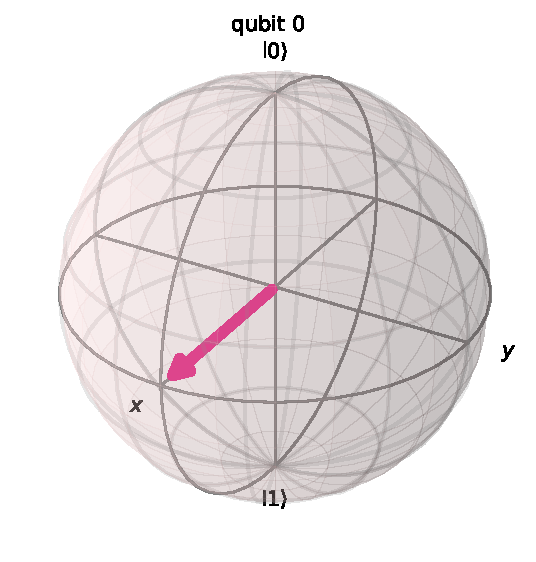
\includegraphics[keepaspectratio]{apostila_files/figure-pdf/cell-18-output-2.pdf}}

\begin{verbatim}

Estado |-⟩ (Fase 180°) - Eixo -X:
\end{verbatim}

\pandocbounded{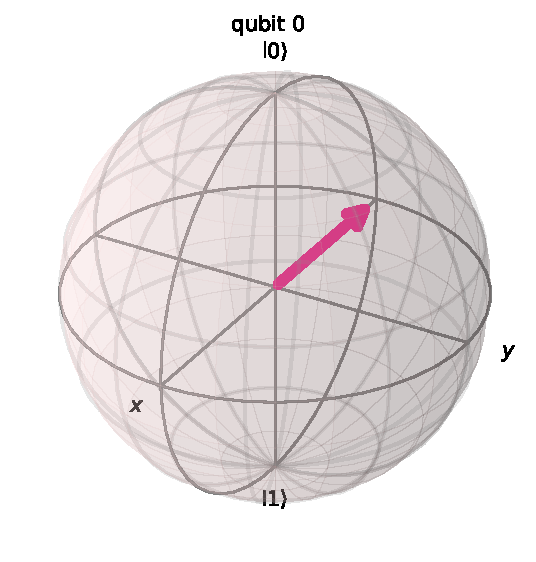
\includegraphics[keepaspectratio]{apostila_files/figure-pdf/cell-18-output-4.pdf}}

\begin{verbatim}

Estado |i+⟩ (Fase 90°) - Eixo +Y:
\end{verbatim}

\pandocbounded{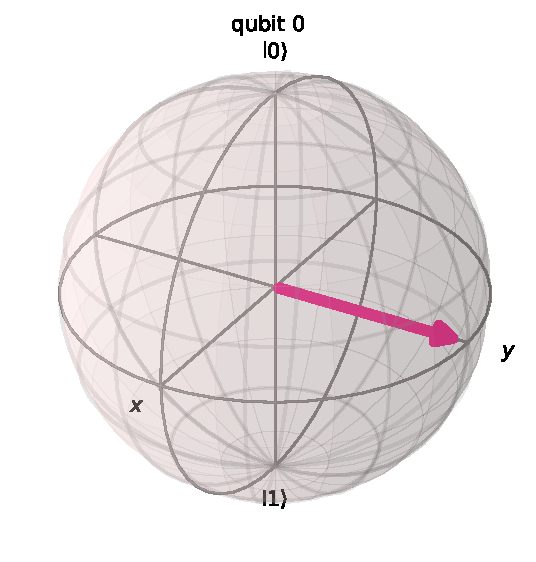
\includegraphics[keepaspectratio]{apostila_files/figure-pdf/cell-18-output-6.pdf}}

\begin{verbatim}

Estado |i-⟩ (Fase 270°) - Eixo -Y:
\end{verbatim}

\pandocbounded{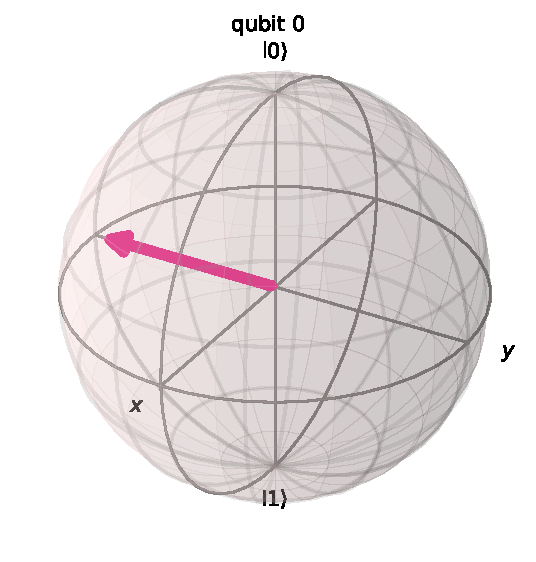
\includegraphics[keepaspectratio]{apostila_files/figure-pdf/cell-18-output-8.pdf}}

\begin{verbatim}

Observe como todos os estados estão no equador da esfera de Bloch
(igual probabilidade de medir 0 ou 1), mas em direções diferentes.
\end{verbatim}

\begin{verbatim}
Estado |+⟩ (Fase 0°) - Eixo +X:
\end{verbatim}

\begin{verbatim}

Estado |-⟩ (Fase 180°) - Eixo -X:
\end{verbatim}

\begin{verbatim}

Estado |i+⟩ (Fase 90°) - Eixo +Y:
\end{verbatim}

\begin{verbatim}

Estado |i-⟩ (Fase 270°) - Eixo -Y:
\end{verbatim}

\begin{verbatim}

Observe como todos os estados estão no equador da esfera de Bloch
(igual probabilidade de medir 0 ou 1), mas em direções diferentes.
\end{verbatim}

\subsection{Demonstração: Efeito da Porta
Z}\label{demonstrauxe7uxe3o-efeito-da-porta-z}

A porta Z inverte a fase do estado \textbar1⟩:

\[Z|+⟩ = Z · \frac{1}{\sqrt{2}}(|0⟩ + |1⟩) = \frac{1}{\sqrt{2}}(|0⟩ - |1⟩) = |-⟩\]

Na esfera de Bloch, isso corresponde a uma rotação de 180° em torno do
eixo Z.

\begin{Shaded}
\begin{Highlighting}[]
\CommentTok{\# Demonstração: Aplicar porta Z em |+⟩}
\NormalTok{estado\_inicial }\OperatorTok{=}\NormalTok{ state\_plus}
\NormalTok{estado\_apos\_Z }\OperatorTok{=}\NormalTok{ Statevector([}\DecValTok{1}\OperatorTok{/}\NormalTok{np.sqrt(}\DecValTok{2}\NormalTok{), }\OperatorTok{{-}}\DecValTok{1}\OperatorTok{/}\NormalTok{np.sqrt(}\DecValTok{2}\NormalTok{)])}

\BuiltInTok{print}\NormalTok{(}\StringTok{"Antes de aplicar a porta Z:"}\NormalTok{)}
\NormalTok{display(plot\_bloch\_multivector(estado\_inicial))}

\BuiltInTok{print}\NormalTok{(}\StringTok{"}\CharTok{\textbackslash{}n}\StringTok{Depois de aplicar a porta Z:"}\NormalTok{)}
\NormalTok{display(plot\_bloch\_multivector(estado\_apos\_Z))}

\BuiltInTok{print}\NormalTok{(}\StringTok{"}\CharTok{\textbackslash{}n}\StringTok{A porta Z rotacionou o estado de +X para {-}X (180° em torno do eixo Z)"}\NormalTok{)}
\end{Highlighting}
\end{Shaded}

\begin{verbatim}
Antes de aplicar a porta Z:
\end{verbatim}

\pandocbounded{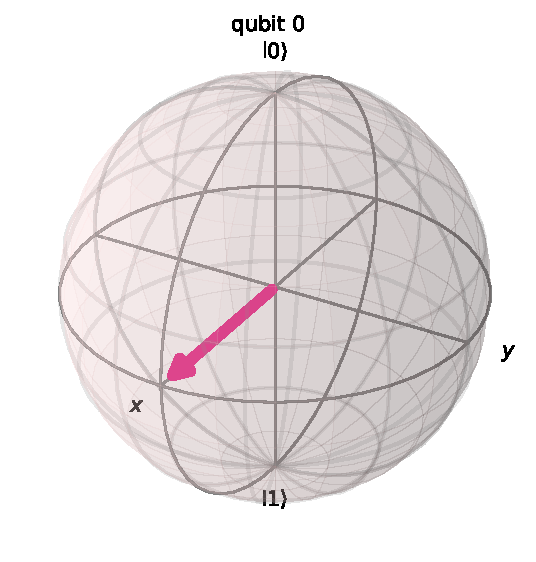
\includegraphics[keepaspectratio]{apostila_files/figure-pdf/cell-19-output-2.pdf}}

\begin{verbatim}

Depois de aplicar a porta Z:
\end{verbatim}

\pandocbounded{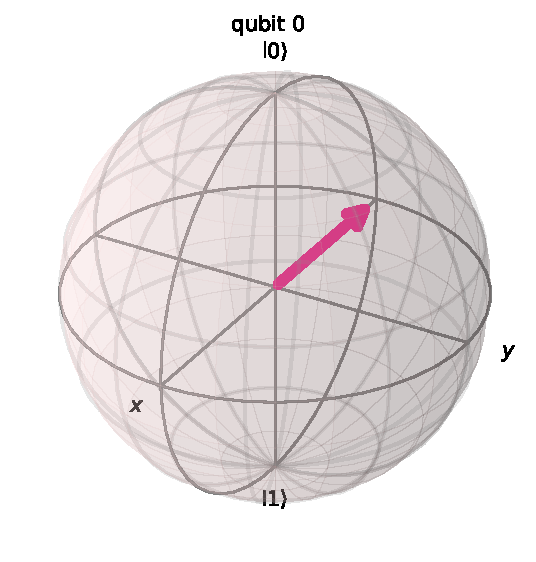
\includegraphics[keepaspectratio]{apostila_files/figure-pdf/cell-19-output-4.pdf}}

\begin{verbatim}

A porta Z rotacionou o estado de +X para -X (180° em torno do eixo Z)
\end{verbatim}

\begin{verbatim}
Antes de aplicar a porta Z:
\end{verbatim}

\begin{verbatim}

Depois de aplicar a porta Z:
\end{verbatim}

\begin{verbatim}

A porta Z rotacionou o estado de +X para -X (180° em torno do eixo Z)
\end{verbatim}

\subsection{Demonstração: Efeito da Porta
S}\label{demonstrauxe7uxe3o-efeito-da-porta-s}

A porta S adiciona uma fase de 90° ao estado \textbar1⟩:

\[S|+⟩ = S · \frac{1}{\sqrt{2}}(|0⟩ + |1⟩) = \frac{1}{\sqrt{2}}(|0⟩ + i|1⟩) = |i+⟩\]

Na esfera de Bloch, isso corresponde a uma rotação de 90° em torno do
eixo Z.

\begin{Shaded}
\begin{Highlighting}[]
\CommentTok{\# Demonstração: Aplicar porta S em |+⟩}
\NormalTok{estado\_inicial }\OperatorTok{=}\NormalTok{ state\_plus}
\NormalTok{estado\_apos\_S }\OperatorTok{=}\NormalTok{ Statevector([}\DecValTok{1}\OperatorTok{/}\NormalTok{np.sqrt(}\DecValTok{2}\NormalTok{), }\OtherTok{1j}\OperatorTok{/}\NormalTok{np.sqrt(}\DecValTok{2}\NormalTok{)])}

\BuiltInTok{print}\NormalTok{(}\StringTok{"Antes de aplicar a porta S:"}\NormalTok{)}
\NormalTok{display(plot\_bloch\_multivector(estado\_inicial))}

\BuiltInTok{print}\NormalTok{(}\StringTok{"}\CharTok{\textbackslash{}n}\StringTok{Depois de aplicar a porta S:"}\NormalTok{)}
\NormalTok{display(plot\_bloch\_multivector(estado\_apos\_S))}

\BuiltInTok{print}\NormalTok{(}\StringTok{"}\CharTok{\textbackslash{}n}\StringTok{A porta S rotacionou o estado de +X para +Y (90° em torno do eixo Z)"}\NormalTok{)}
\end{Highlighting}
\end{Shaded}

\begin{verbatim}
Antes de aplicar a porta S:
\end{verbatim}

\pandocbounded{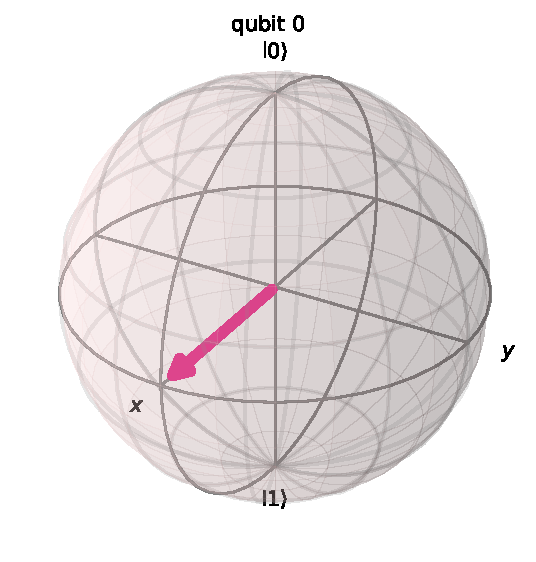
\includegraphics[keepaspectratio]{apostila_files/figure-pdf/cell-20-output-2.pdf}}

\begin{verbatim}

Depois de aplicar a porta S:
\end{verbatim}

\pandocbounded{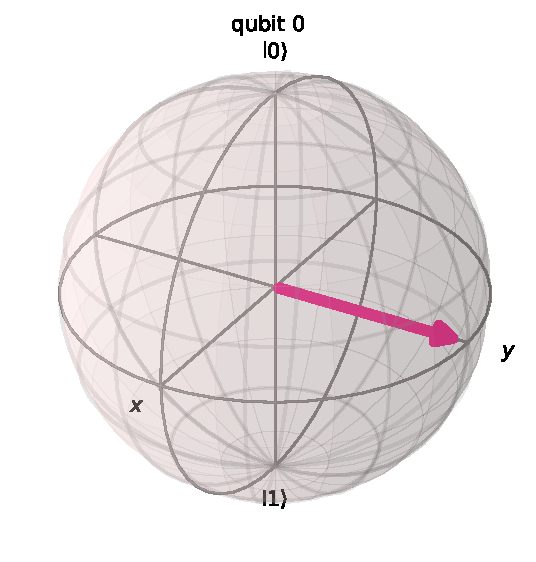
\includegraphics[keepaspectratio]{apostila_files/figure-pdf/cell-20-output-4.pdf}}

\begin{verbatim}

A porta S rotacionou o estado de +X para +Y (90° em torno do eixo Z)
\end{verbatim}

\begin{verbatim}
Antes de aplicar a porta S:
\end{verbatim}

\begin{verbatim}

Depois de aplicar a porta S:
\end{verbatim}

\begin{verbatim}

A porta S rotacionou o estado de +X para +Y (90° em torno do eixo Z)
\end{verbatim}

\subsection{Visualização com
Q-Sphere}\label{visualizauxe7uxe3o-com-q-sphere}

O Q-Sphere é outra forma de visualizar estados quânticos, onde as
\textbf{cores} representam as fases: - \textbf{Verde/Azul claro}: Fase
positiva (0° a 90°) - \textbf{Vermelho/Laranja}: Fase negativa (180° a
270°) - \textbf{Tamanho das esferas}: Magnitude da amplitude

\begin{Shaded}
\begin{Highlighting}[]
\CommentTok{\# Visualizar os mesmos estados no Q{-}Sphere}
\BuiltInTok{print}\NormalTok{(}\StringTok{"Estado |+⟩ {-} Fase 0°:"}\NormalTok{)}
\NormalTok{display(plot\_state\_qsphere(state\_plus))}

\BuiltInTok{print}\NormalTok{(}\StringTok{"}\CharTok{\textbackslash{}n}\StringTok{Estado |{-}⟩ {-} Fase 180°:"}\NormalTok{)}
\NormalTok{display(plot\_state\_qsphere(state\_minus))}

\BuiltInTok{print}\NormalTok{(}\StringTok{"}\CharTok{\textbackslash{}n}\StringTok{Estado |i+⟩ {-} Fase 90°:"}\NormalTok{)}
\NormalTok{display(plot\_state\_qsphere(state\_i\_plus))}

\BuiltInTok{print}\NormalTok{(}\StringTok{"}\CharTok{\textbackslash{}n}\StringTok{Estado |i{-}⟩ {-} Fase 270°:"}\NormalTok{)}
\NormalTok{display(plot\_state\_qsphere(state\_i\_minus))}

\BuiltInTok{print}\NormalTok{(}\StringTok{"}\CharTok{\textbackslash{}n}\StringTok{No Q{-}Sphere, observe a mudança de cores indicando diferentes fases."}\NormalTok{)}
\end{Highlighting}
\end{Shaded}

\begin{verbatim}
Estado |+⟩ - Fase 0°:
\end{verbatim}

\pandocbounded{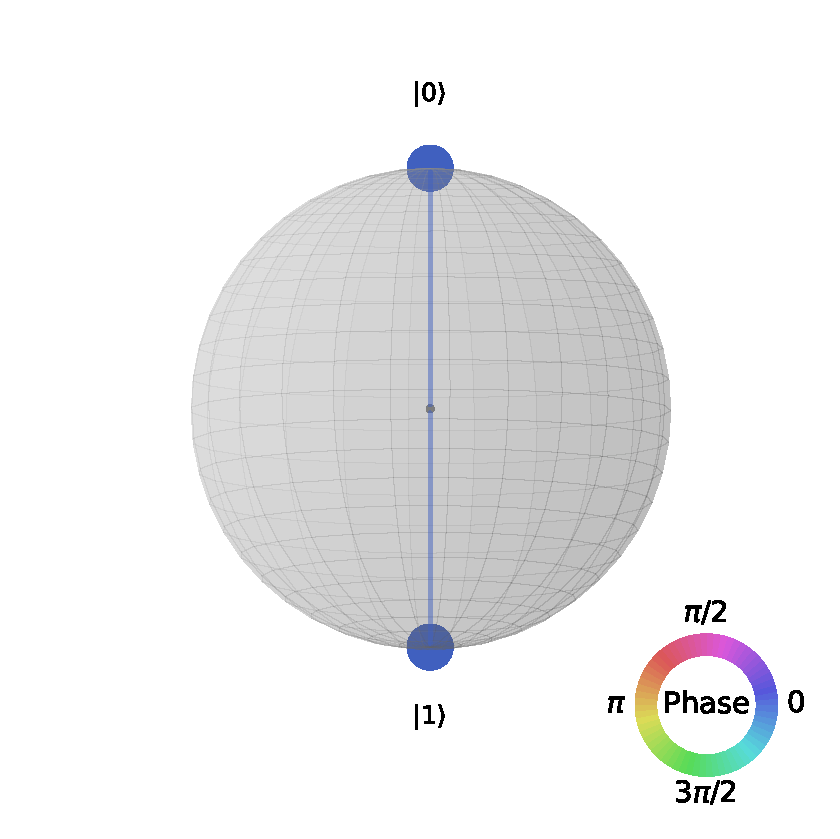
\includegraphics[keepaspectratio]{apostila_files/figure-pdf/cell-21-output-2.pdf}}

\begin{verbatim}

Estado |-⟩ - Fase 180°:
\end{verbatim}

\pandocbounded{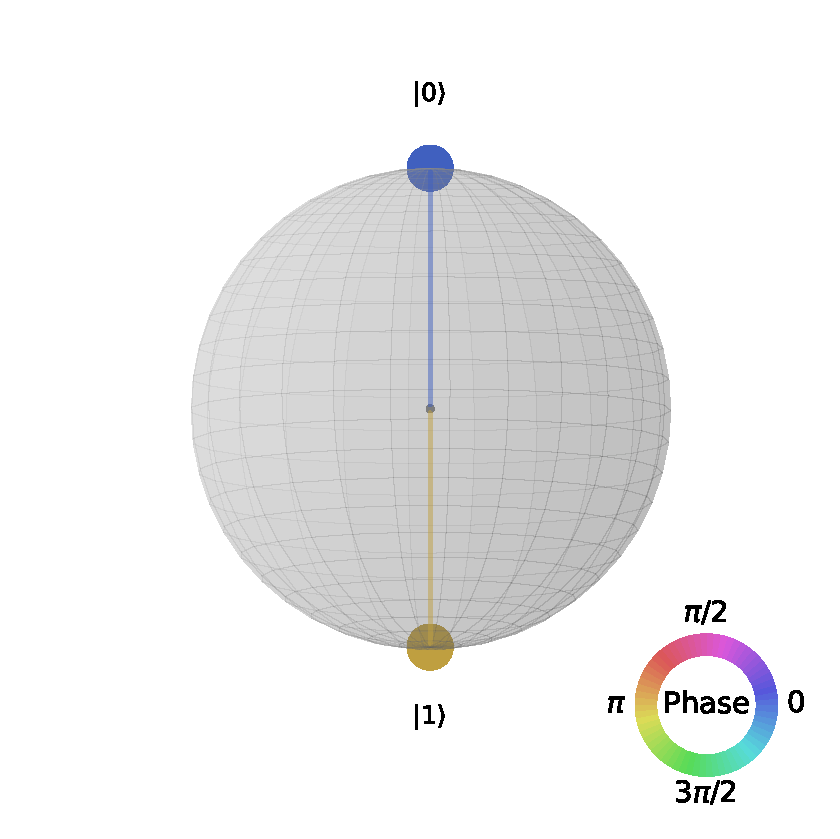
\includegraphics[keepaspectratio]{apostila_files/figure-pdf/cell-21-output-4.pdf}}

\begin{verbatim}

Estado |i+⟩ - Fase 90°:
\end{verbatim}

\pandocbounded{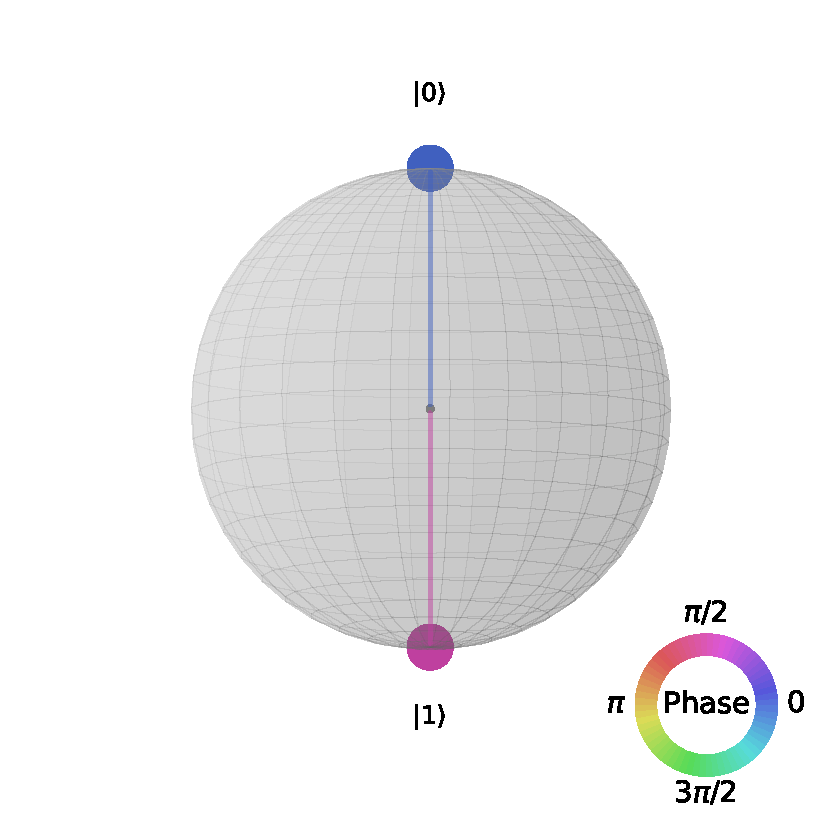
\includegraphics[keepaspectratio]{apostila_files/figure-pdf/cell-21-output-6.pdf}}

\begin{verbatim}

Estado |i-⟩ - Fase 270°:
\end{verbatim}

\pandocbounded{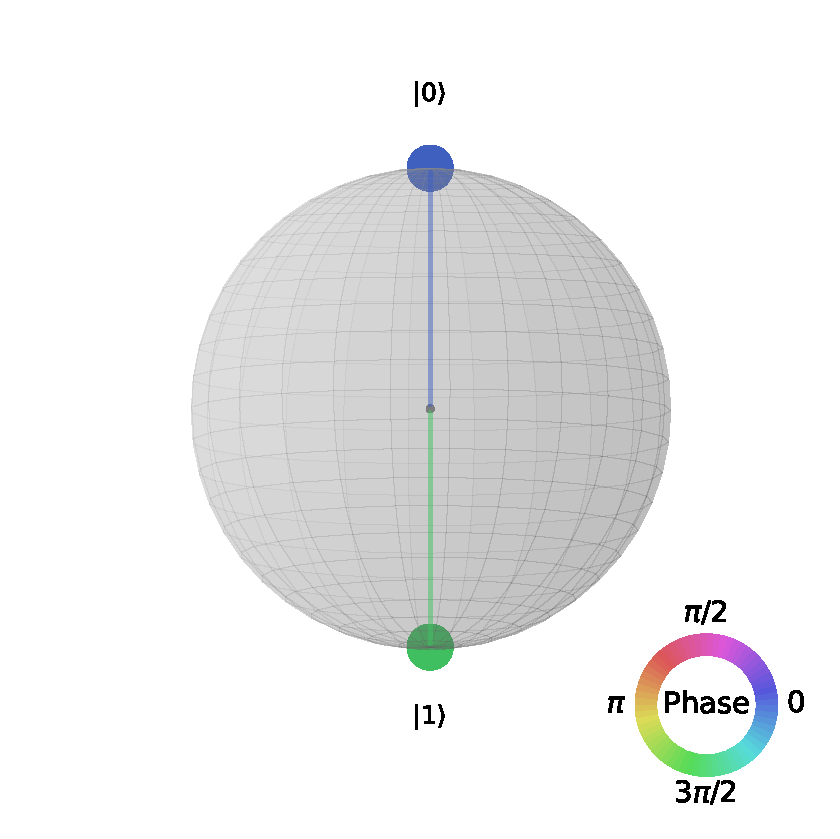
\includegraphics[keepaspectratio]{apostila_files/figure-pdf/cell-21-output-8.pdf}}

\begin{verbatim}

No Q-Sphere, observe a mudança de cores indicando diferentes fases.
\end{verbatim}

\begin{verbatim}
Estado |+⟩ - Fase 0°:
\end{verbatim}

\begin{verbatim}

Estado |-⟩ - Fase 180°:
\end{verbatim}

\begin{verbatim}

Estado |i+⟩ - Fase 90°:
\end{verbatim}

\begin{verbatim}

Estado |i-⟩ - Fase 270°:
\end{verbatim}

\begin{verbatim}

No Q-Sphere, observe a mudança de cores indicando diferentes fases.
\end{verbatim}

\subsection{🧪 Experimento Interativo: Crie seu próprio estado com
fase!}\label{experimento-interativo-crie-seu-pruxf3prio-estado-com-fase}

Modifique o ângulo θ abaixo para criar diferentes estados de
superposição com fases variadas:

\subsection{📊 Resumo: Por que a Fase é
Importante?}\label{resumo-por-que-a-fase-uxe9-importante}

\begin{longtable}[]{@{}
  >{\raggedright\arraybackslash}p{(\linewidth - 4\tabcolsep) * \real{0.2778}}
  >{\raggedright\arraybackslash}p{(\linewidth - 4\tabcolsep) * \real{0.3611}}
  >{\raggedright\arraybackslash}p{(\linewidth - 4\tabcolsep) * \real{0.3611}}@{}}
\toprule\noalign{}
\begin{minipage}[b]{\linewidth}\raggedright
Conceito
\end{minipage} & \begin{minipage}[b]{\linewidth}\raggedright
Observável?
\end{minipage} & \begin{minipage}[b]{\linewidth}\raggedright
Importância
\end{minipage} \\
\midrule\noalign{}
\endhead
\bottomrule\noalign{}
\endlastfoot
\textbf{Fase Global} & ❌ Não & Irrelevante matematicamente \\
\textbf{Fase Relativa} & ✅ Sim (através de interferência) & Essencial
para algoritmos quânticos \\
\textbf{Porta Z} & Modifica fase & Inverte fase de \textbar1⟩ (180°) \\
\textbf{Porta S} & Modifica fase & Adiciona 90° de fase a \textbar1⟩ \\
\textbf{Porta T} & Modifica fase & Adiciona 45° de fase a \textbar1⟩ \\
\end{longtable}

A fase quântica é fundamental para: - 🔄 \textbf{Interferência
quântica}: Estados podem interferir construtivamente ou destrutivamente
- 🎯 \textbf{Algoritmos quânticos}: Grover, Shor, e outros dependem de
manipulação precisa de fases - 🔗 \textbf{Emaranhamento}: Estados
emaranhados têm relações de fase específicas - ⚡ \textbf{Phase
Kickback}: Técnica usada em oráculos quânticos (veremos em notebooks
avançados)

\begin{Shaded}
\begin{Highlighting}[]
\CommentTok{\# Experimente diferentes valores de theta (em graus)}
\NormalTok{theta\_graus }\OperatorTok{=} \DecValTok{45}  \CommentTok{\# Modifique este valor: 0, 45, 90, 135, 180, 225, 270, 315...}
\NormalTok{theta\_rad }\OperatorTok{=}\NormalTok{ np.deg2rad(theta\_graus)}

\CommentTok{\# Criar estado com fase customizada}
\NormalTok{estado\_custom }\OperatorTok{=}\NormalTok{ Statevector([}\DecValTok{1}\OperatorTok{/}\NormalTok{np.sqrt(}\DecValTok{2}\NormalTok{), np.exp(}\OtherTok{1j} \OperatorTok{*}\NormalTok{ theta\_rad)}\OperatorTok{/}\NormalTok{np.sqrt(}\DecValTok{2}\NormalTok{)])}

\CommentTok{\# Mostrar o estado matematicamente}
\BuiltInTok{print}\NormalTok{(}\SpecialStringTok{f"Estado criado: |ψ⟩ = 1/√2 (|0⟩ + e\^{}(i·}\SpecialCharTok{\{}\NormalTok{theta\_graus}\SpecialCharTok{\}}\SpecialStringTok{°)|1⟩)"}\NormalTok{)}
\BuiltInTok{print}\NormalTok{(}\SpecialStringTok{f"Componente |0⟩: }\SpecialCharTok{\{}\NormalTok{estado\_custom}\SpecialCharTok{.}\NormalTok{data[}\DecValTok{0}\NormalTok{]}\SpecialCharTok{\}}\SpecialStringTok{"}\NormalTok{)}
\BuiltInTok{print}\NormalTok{(}\SpecialStringTok{f"Componente |1⟩: }\SpecialCharTok{\{}\NormalTok{estado\_custom}\SpecialCharTok{.}\NormalTok{data[}\DecValTok{1}\NormalTok{]}\SpecialCharTok{\}}\SpecialStringTok{"}\NormalTok{)}
\BuiltInTok{print}\NormalTok{(}\SpecialStringTok{f"Fase relativa: }\SpecialCharTok{\{}\NormalTok{theta\_graus}\SpecialCharTok{\}}\SpecialStringTok{°}\CharTok{\textbackslash{}n}\SpecialStringTok{"}\NormalTok{)}

\CommentTok{\# Visualizar na Esfera de Bloch}
\BuiltInTok{print}\NormalTok{(}\SpecialStringTok{f"Esfera de Bloch {-} Fase θ = }\SpecialCharTok{\{}\NormalTok{theta\_graus}\SpecialCharTok{\}}\SpecialStringTok{°:"}\NormalTok{)}
\NormalTok{display(plot\_bloch\_multivector(estado\_custom))}

\CommentTok{\# Visualizar no Q{-}Sphere}
\BuiltInTok{print}\NormalTok{(}\SpecialStringTok{f"}\CharTok{\textbackslash{}n}\SpecialStringTok{Q{-}Sphere {-} Fase θ = }\SpecialCharTok{\{}\NormalTok{theta\_graus}\SpecialCharTok{\}}\SpecialStringTok{°:"}\NormalTok{)}
\NormalTok{display(plot\_state\_qsphere(estado\_custom))  }
\end{Highlighting}
\end{Shaded}

\begin{verbatim}
Estado criado: |ψ⟩ = 1/√2 (|0⟩ + e^(i·45°)|1⟩)
Componente |0⟩: (0.7071067811865475+0j)
Componente |1⟩: (0.5+0.4999999999999999j)
Fase relativa: 45°

Esfera de Bloch - Fase θ = 45°:
\end{verbatim}

\pandocbounded{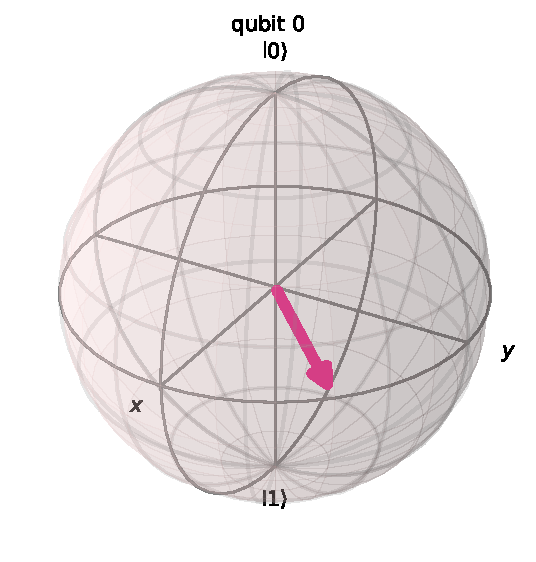
\includegraphics[keepaspectratio]{apostila_files/figure-pdf/cell-22-output-2.pdf}}

\begin{verbatim}

Q-Sphere - Fase θ = 45°:
\end{verbatim}

\pandocbounded{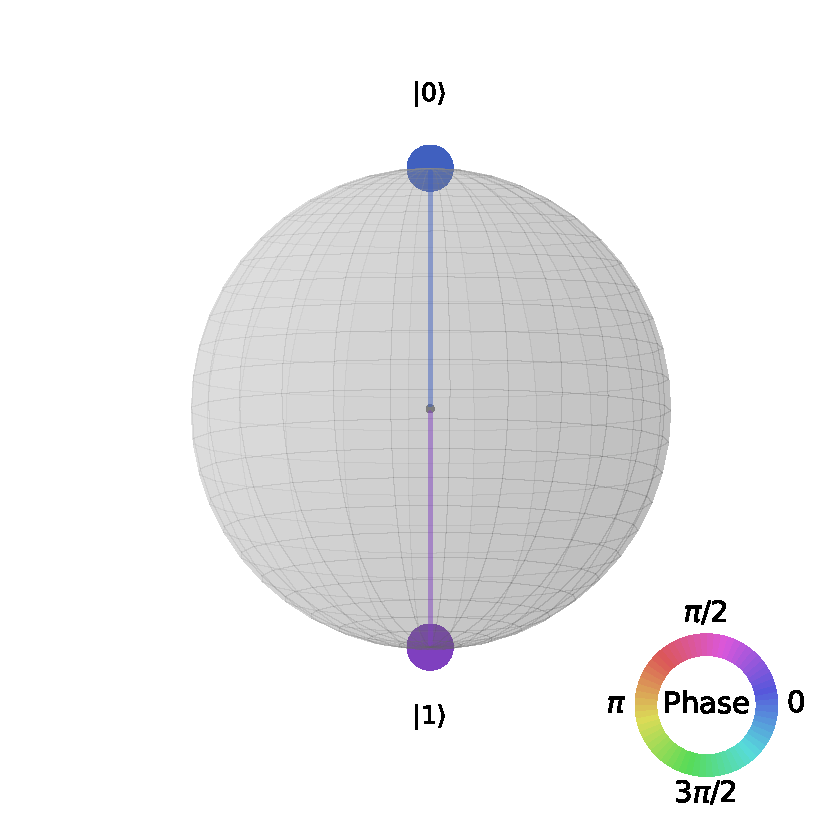
\includegraphics[keepaspectratio]{apostila_files/figure-pdf/cell-22-output-4.pdf}}

\begin{verbatim}
Estado criado: |ψ⟩ = 1/√2 (|0⟩ + e^(i·45°)|1⟩)
Componente |0⟩: (0.7071067811865475+0j)
Componente |1⟩: (0.5+0.5j)
Fase relativa: 45°

Esfera de Bloch - Fase θ = 45°:
\end{verbatim}

\begin{verbatim}

Q-Sphere - Fase θ = 45°:
\end{verbatim}

\section{🔄 Portas de Rotação
Parametrizadas}\label{portas-de-rotauxe7uxe3o-parametrizadas}

Até agora vimos portas com ângulos fixos (Z = 180°, S = 90°, T = 45°).
Mas em muitos algoritmos quânticos --- especialmente em \textbf{Machine
Learning Quântico} e \textbf{Circuitos Variacionais} --- precisamos de
portas que aceitem \textbf{qualquer ângulo θ como parâmetro}.

Essas são as \textbf{portas de rotação parametrizadas}: \textbf{RX(θ)},
\textbf{RY(θ)} e \textbf{RZ(θ)}.

\subsection{🎯 Por que são
importantes?}\label{por-que-suxe3o-importantes}

\begin{itemize}
\tightlist
\item
  \textbf{VQC (Variational Quantum Classifier)}: Usa RY e RZ para
  codificar dados clássicos em estados quânticos
\item
  \textbf{Ansatz variacional}: RY é a porta mais comum em ansatz como
  \texttt{RealAmplitudes}
\item
  \textbf{Otimização quântica}: Os ângulos θ são ajustados
  iterativamente para minimizar uma função custo
\item
  \textbf{Controle fino}: Permitem explorar qualquer ponto na Esfera de
  Bloch
\end{itemize}

\subsection{📐 As Três Portas de
Rotação}\label{as-truxeas-portas-de-rotauxe7uxe3o}

Cada porta rotaciona o qubit em torno de um eixo da Esfera de Bloch:

\begin{longtable}[]{@{}
  >{\raggedright\arraybackslash}p{(\linewidth - 6\tabcolsep) * \real{0.1667}}
  >{\raggedright\arraybackslash}p{(\linewidth - 6\tabcolsep) * \real{0.3810}}
  >{\raggedright\arraybackslash}p{(\linewidth - 6\tabcolsep) * \real{0.1905}}
  >{\raggedright\arraybackslash}p{(\linewidth - 6\tabcolsep) * \real{0.2619}}@{}}
\toprule\noalign{}
\begin{minipage}[b]{\linewidth}\raggedright
Porta
\end{minipage} & \begin{minipage}[b]{\linewidth}\raggedright
Eixo de Rotação
\end{minipage} & \begin{minipage}[b]{\linewidth}\raggedright
Matriz
\end{minipage} & \begin{minipage}[b]{\linewidth}\raggedright
Uso Comum
\end{minipage} \\
\midrule\noalign{}
\endhead
\bottomrule\noalign{}
\endlastfoot
\textbf{RX(θ)} & Eixo X &
\(\begin{bmatrix} \cos(\frac{\theta}{2}) & -i\sin(\frac{\theta}{2}) \\ -i\sin(\frac{\theta}{2}) & \cos(\frac{\theta}{2}) \end{bmatrix}\)
& Rotações no plano YZ \\
\textbf{RY(θ)} & Eixo Y &
\(\begin{bmatrix} \cos(\frac{\theta}{2}) & -\sin(\frac{\theta}{2}) \\ \sin(\frac{\theta}{2}) & \cos(\frac{\theta}{2}) \end{bmatrix}\)
& Codificação de dados, Ansatz \\
\textbf{RZ(θ)} & Eixo Z &
\(\begin{bmatrix} e^{-i\frac{\theta}{2}} & 0 \\ 0 & e^{i\frac{\theta}{2}} \end{bmatrix}\)
& Ajuste de fase, Feature Maps \\
\end{longtable}

\textbf{Observação importante:} O ângulo nas matrizes é \textbf{θ/2}
(metade do ângulo de rotação na Esfera de Bloch). Isso é uma convenção
da mecânica quântica relacionada ao grupo SU(2).

\begin{Shaded}
\begin{Highlighting}[]
\CommentTok{\# Definir as portas de rotação parametrizadas}
\ImportTok{import}\NormalTok{ numpy }\ImportTok{as}\NormalTok{ np}
\ImportTok{import}\NormalTok{ sympy }\ImportTok{as}\NormalTok{ sp}
\ImportTok{from}\NormalTok{ sympy }\ImportTok{import}\NormalTok{ Matrix, symbols, cos, sin, exp, I, pi, latex}
\ImportTok{from}\NormalTok{ IPython.display }\ImportTok{import}\NormalTok{ display, Markdown}

\CommentTok{\# Definir o símbolo theta}
\NormalTok{theta }\OperatorTok{=}\NormalTok{ symbols(}\StringTok{\textquotesingle{}theta\textquotesingle{}}\NormalTok{, real}\OperatorTok{=}\VariableTok{True}\NormalTok{)}

\CommentTok{\# Porta RX(θ) {-} Rotação em torno do eixo X}
\NormalTok{RX }\OperatorTok{=}\NormalTok{ Matrix([}
\NormalTok{    [cos(theta}\OperatorTok{/}\DecValTok{2}\NormalTok{), }\OperatorTok{{-}}\NormalTok{I}\OperatorTok{*}\NormalTok{sin(theta}\OperatorTok{/}\DecValTok{2}\NormalTok{)],}
\NormalTok{    [}\OperatorTok{{-}}\NormalTok{I}\OperatorTok{*}\NormalTok{sin(theta}\OperatorTok{/}\DecValTok{2}\NormalTok{), cos(theta}\OperatorTok{/}\DecValTok{2}\NormalTok{)]}
\NormalTok{])}

\CommentTok{\# Porta RY(θ) {-} Rotação em torno do eixo Y  }
\NormalTok{RY }\OperatorTok{=}\NormalTok{ Matrix([}
\NormalTok{    [cos(theta}\OperatorTok{/}\DecValTok{2}\NormalTok{), }\OperatorTok{{-}}\NormalTok{sin(theta}\OperatorTok{/}\DecValTok{2}\NormalTok{)],}
\NormalTok{    [sin(theta}\OperatorTok{/}\DecValTok{2}\NormalTok{), cos(theta}\OperatorTok{/}\DecValTok{2}\NormalTok{)]}
\NormalTok{])}

\CommentTok{\# Porta RZ(θ) {-} Rotação em torno do eixo Z}
\NormalTok{RZ }\OperatorTok{=}\NormalTok{ Matrix([}
\NormalTok{    [exp(}\OperatorTok{{-}}\NormalTok{I}\OperatorTok{*}\NormalTok{theta}\OperatorTok{/}\DecValTok{2}\NormalTok{), }\DecValTok{0}\NormalTok{],}
\NormalTok{    [}\DecValTok{0}\NormalTok{, exp(I}\OperatorTok{*}\NormalTok{theta}\OperatorTok{/}\DecValTok{2}\NormalTok{)]}
\NormalTok{])}

\NormalTok{display(Markdown(}\SpecialStringTok{f"\#\#\# Matrizes das Portas de Rotação"}\NormalTok{))}
\NormalTok{display(Markdown(}\SpecialStringTok{f"**RX(θ)** {-} Rotação no eixo X:"}\NormalTok{))}
\NormalTok{display(Markdown(}\SpecialStringTok{f"$$ RX(}\CharTok{\textbackslash{}\textbackslash{}}\SpecialStringTok{theta) = }\SpecialCharTok{\{}\NormalTok{latex(RX)}\SpecialCharTok{\}}\SpecialStringTok{ $$"}\NormalTok{))}
\NormalTok{display(Markdown(}\SpecialStringTok{f"**RY(θ)** {-} Rotação no eixo Y:"}\NormalTok{))}
\NormalTok{display(Markdown(}\SpecialStringTok{f"$$ RY(}\CharTok{\textbackslash{}\textbackslash{}}\SpecialStringTok{theta) = }\SpecialCharTok{\{}\NormalTok{latex(RY)}\SpecialCharTok{\}}\SpecialStringTok{ $$"}\NormalTok{))}
\NormalTok{display(Markdown(}\SpecialStringTok{f"**RZ(θ)** {-} Rotação no eixo Z:"}\NormalTok{))}
\NormalTok{display(Markdown(}\SpecialStringTok{f"$$ RZ(}\CharTok{\textbackslash{}\textbackslash{}}\SpecialStringTok{theta) = }\SpecialCharTok{\{}\NormalTok{latex(RZ)}\SpecialCharTok{\}}\SpecialStringTok{ $$"}\NormalTok{))}
\end{Highlighting}
\end{Shaded}

\subsection{Matrizes das Portas de
Rotação}\label{matrizes-das-portas-de-rotauxe7uxe3o}

\textbf{RX(θ)} - Rotação no eixo X:

\[ RX(\theta) = \left[\begin{matrix}\cos{\left(\frac{\theta}{2} \right)} & - i \sin{\left(\frac{\theta}{2} \right)}\\- i \sin{\left(\frac{\theta}{2} \right)} & \cos{\left(\frac{\theta}{2} \right)}\end{matrix}\right] \]

\textbf{RY(θ)} - Rotação no eixo Y:

\[ RY(\theta) = \left[\begin{matrix}\cos{\left(\frac{\theta}{2} \right)} & - \sin{\left(\frac{\theta}{2} \right)}\\\sin{\left(\frac{\theta}{2} \right)} & \cos{\left(\frac{\theta}{2} \right)}\end{matrix}\right] \]

\textbf{RZ(θ)} - Rotação no eixo Z:

\[ RZ(\theta) = \left[\begin{matrix}e^{- \frac{i \theta}{2}} & 0\\0 & e^{\frac{i \theta}{2}}\end{matrix}\right] \]

\subsection{🔬 Exemplo 1: Porta RY - A mais usada em Machine
Learning}\label{exemplo-1-porta-ry---a-mais-usada-em-machine-learning}

A porta \textbf{RY(θ)} é especialmente importante porque: - Não introduz
números complexos (apenas senos e cossenos reais) - É a porta padrão no
ansatz \texttt{RealAmplitudes} do Qiskit - Permite mapear diretamente
dados clássicos em ângulos quânticos

Vamos aplicar RY com diferentes ângulos ao estado \textbar0⟩:

\begin{Shaded}
\begin{Highlighting}[]
\ImportTok{from}\NormalTok{ qiskit }\ImportTok{import}\NormalTok{ QuantumCircuit}
\ImportTok{from}\NormalTok{ qiskit.quantum\_info }\ImportTok{import}\NormalTok{ Statevector}
\ImportTok{from}\NormalTok{ qiskit.visualization }\ImportTok{import}\NormalTok{ plot\_bloch\_multivector}
\ImportTok{import}\NormalTok{ matplotlib.pyplot }\ImportTok{as}\NormalTok{ plt}

\CommentTok{\# Testar RY com diferentes ângulos}
\NormalTok{angulos }\OperatorTok{=}\NormalTok{ [}\DecValTok{0}\NormalTok{, np.pi}\OperatorTok{/}\DecValTok{4}\NormalTok{, np.pi}\OperatorTok{/}\DecValTok{2}\NormalTok{, }\DecValTok{3}\OperatorTok{*}\NormalTok{np.pi}\OperatorTok{/}\DecValTok{4}\NormalTok{, np.pi]}
\NormalTok{nomes }\OperatorTok{=}\NormalTok{ [}\StringTok{\textquotesingle{}0°\textquotesingle{}}\NormalTok{, }\StringTok{\textquotesingle{}45°\textquotesingle{}}\NormalTok{, }\StringTok{\textquotesingle{}90°\textquotesingle{}}\NormalTok{, }\StringTok{\textquotesingle{}135°\textquotesingle{}}\NormalTok{, }\StringTok{\textquotesingle{}180°\textquotesingle{}}\NormalTok{]}

\BuiltInTok{print}\NormalTok{(}\StringTok{"="} \OperatorTok{*} \DecValTok{70}\NormalTok{)}
\BuiltInTok{print}\NormalTok{(}\StringTok{"PORTA RY: Rotação em torno do eixo Y"}\NormalTok{)}
\BuiltInTok{print}\NormalTok{(}\StringTok{"="} \OperatorTok{*} \DecValTok{70}\NormalTok{)}

\NormalTok{fig, axes }\OperatorTok{=}\NormalTok{ plt.subplots(}\DecValTok{1}\NormalTok{, }\DecValTok{5}\NormalTok{, figsize}\OperatorTok{=}\NormalTok{(}\DecValTok{20}\NormalTok{, }\DecValTok{4}\NormalTok{), subplot\_kw}\OperatorTok{=}\NormalTok{\{}\StringTok{\textquotesingle{}projection\textquotesingle{}}\NormalTok{: }\StringTok{\textquotesingle{}3d\textquotesingle{}}\NormalTok{\})}

\ControlFlowTok{for}\NormalTok{ i, (angulo, nome) }\KeywordTok{in} \BuiltInTok{enumerate}\NormalTok{(}\BuiltInTok{zip}\NormalTok{(angulos, nomes)):}
    \CommentTok{\# Criar circuito}
\NormalTok{    qc }\OperatorTok{=}\NormalTok{ QuantumCircuit(}\DecValTok{1}\NormalTok{)}
\NormalTok{    qc.ry(angulo, }\DecValTok{0}\NormalTok{)}
    
    \CommentTok{\# Obter estado}
\NormalTok{    state }\OperatorTok{=}\NormalTok{ Statevector(qc)}
    
    \CommentTok{\# Calcular amplitudes}
\NormalTok{    alpha }\OperatorTok{=}\NormalTok{ state.data[}\DecValTok{0}\NormalTok{]}
\NormalTok{    beta }\OperatorTok{=}\NormalTok{ state.data[}\DecValTok{1}\NormalTok{]}
    
    \BuiltInTok{print}\NormalTok{(}\SpecialStringTok{f"}\CharTok{\textbackslash{}n}\SpecialCharTok{\{}\NormalTok{nome}\SpecialCharTok{\}}\SpecialStringTok{ (θ = }\SpecialCharTok{\{}\NormalTok{angulo}\SpecialCharTok{:.4f\}}\SpecialStringTok{ rad):"}\NormalTok{)}
    \BuiltInTok{print}\NormalTok{(}\SpecialStringTok{f"  RY(}\SpecialCharTok{\{}\NormalTok{angulo}\SpecialCharTok{:.4f\}}\SpecialStringTok{)|0⟩ = }\SpecialCharTok{\{}\NormalTok{alpha}\SpecialCharTok{:.4f\}}\SpecialStringTok{|0⟩ + }\SpecialCharTok{\{}\NormalTok{beta}\SpecialCharTok{:.4f\}}\SpecialStringTok{|1⟩"}\NormalTok{)}
    \BuiltInTok{print}\NormalTok{(}\SpecialStringTok{f"  Probabilidades: P(0) = }\SpecialCharTok{\{}\BuiltInTok{abs}\NormalTok{(alpha)}\OperatorTok{**}\DecValTok{2}\SpecialCharTok{:.4f\}}\SpecialStringTok{, P(1) = }\SpecialCharTok{\{}\BuiltInTok{abs}\NormalTok{(beta)}\OperatorTok{**}\DecValTok{2}\SpecialCharTok{:.4f\}}\SpecialStringTok{"}\NormalTok{)}
    
    \CommentTok{\# Plotar na Esfera de Bloch}
    \ImportTok{from}\NormalTok{ qiskit.visualization }\ImportTok{import}\NormalTok{ plot\_bloch\_vector}
    
    \CommentTok{\# Converter estado em coordenadas de Bloch}
\NormalTok{    theta\_bloch }\OperatorTok{=} \DecValTok{2} \OperatorTok{*}\NormalTok{ angulo  }\CommentTok{\# Dobrar o ângulo para coordenadas de Bloch}
\NormalTok{    x }\OperatorTok{=}\NormalTok{ np.sin(theta\_bloch)}
\NormalTok{    y }\OperatorTok{=} \DecValTok{0}  \CommentTok{\# RY mantém y=0 (rotação no plano XZ)}
\NormalTok{    z }\OperatorTok{=}\NormalTok{ np.cos(theta\_bloch)}
    
\NormalTok{    plot\_bloch\_vector([x, y, z], ax}\OperatorTok{=}\NormalTok{axes[i], title}\OperatorTok{=}\SpecialStringTok{f\textquotesingle{}RY(}\SpecialCharTok{\{}\NormalTok{nome}\SpecialCharTok{\}}\SpecialStringTok{)\textquotesingle{}}\NormalTok{)}

\NormalTok{plt.subplots\_adjust(wspace}\OperatorTok{=}\FloatTok{0.4}\NormalTok{)}
\NormalTok{plt.show()}

\BuiltInTok{print}\NormalTok{(}\StringTok{"}\CharTok{\textbackslash{}n}\StringTok{"} \OperatorTok{+} \StringTok{"="} \OperatorTok{*} \DecValTok{70}\NormalTok{)}
\BuiltInTok{print}\NormalTok{(}\StringTok{"Observações:"}\NormalTok{)}
\BuiltInTok{print}\NormalTok{(}\StringTok{"  • RY(0°) = |0⟩ (polo norte)"}\NormalTok{)}
\BuiltInTok{print}\NormalTok{(}\StringTok{"  • RY(90°) = |+⟩ (equador)"}\NormalTok{)  }
\BuiltInTok{print}\NormalTok{(}\StringTok{"  • RY(180°) = |1⟩ (polo sul)"}\NormalTok{)}
\BuiltInTok{print}\NormalTok{(}\StringTok{"  • Todos os estados estão no plano XZ (y = 0)"}\NormalTok{)}
\BuiltInTok{print}\NormalTok{(}\StringTok{"="} \OperatorTok{*} \DecValTok{70}\NormalTok{)}
\end{Highlighting}
\end{Shaded}

\begin{verbatim}
======================================================================
PORTA RY: Rotação em torno do eixo Y
======================================================================

0° (θ = 0.0000 rad):
  RY(0.0000)|0⟩ = 1.0000+0.0000j|0⟩ + 0.0000+0.0000j|1⟩
  Probabilidades: P(0) = 1.0000, P(1) = 0.0000

45° (θ = 0.7854 rad):
  RY(0.7854)|0⟩ = 0.9239+0.0000j|0⟩ + 0.3827+0.0000j|1⟩
  Probabilidades: P(0) = 0.8536, P(1) = 0.1464

90° (θ = 1.5708 rad):
  RY(1.5708)|0⟩ = 0.7071+0.0000j|0⟩ + 0.7071+0.0000j|1⟩
  Probabilidades: P(0) = 0.5000, P(1) = 0.5000

135° (θ = 2.3562 rad):
  RY(2.3562)|0⟩ = 0.3827+0.0000j|0⟩ + 0.9239+0.0000j|1⟩
  Probabilidades: P(0) = 0.1464, P(1) = 0.8536

180° (θ = 3.1416 rad):
  RY(3.1416)|0⟩ = 0.0000+0.0000j|0⟩ + 1.0000+0.0000j|1⟩
  Probabilidades: P(0) = 0.0000, P(1) = 1.0000
\end{verbatim}

\pandocbounded{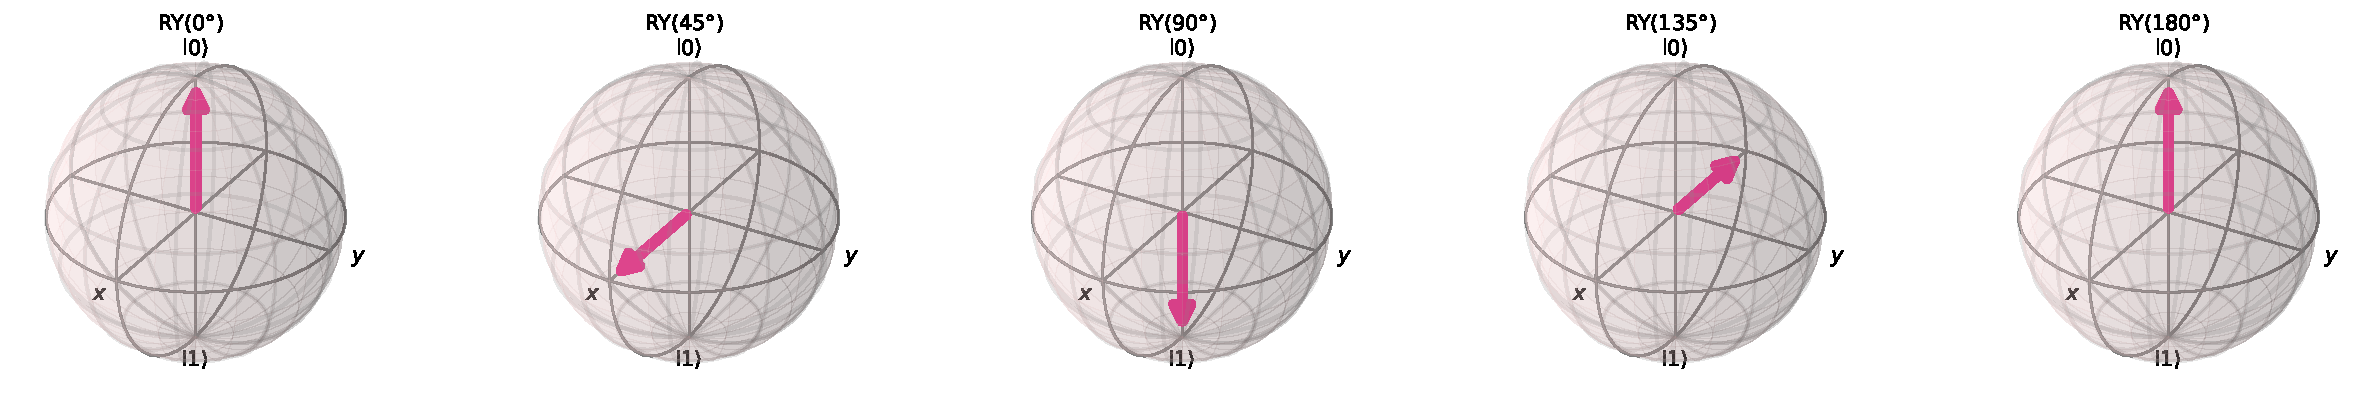
\includegraphics[keepaspectratio]{apostila_files/figure-pdf/cell-24-output-2.pdf}}

\begin{verbatim}

======================================================================
Observações:
  • RY(0°) = |0⟩ (polo norte)
  • RY(90°) = |+⟩ (equador)
  • RY(180°) = |1⟩ (polo sul)
  • Todos os estados estão no plano XZ (y = 0)
======================================================================
\end{verbatim}

\begin{verbatim}
======================================================================
PORTA RY: Rotação em torno do eixo Y
======================================================================

0° (θ = 0.0000 rad):
  RY(0.0000)|0⟩ = 1.0000+0.0000j|0⟩ + 0.0000+0.0000j|1⟩
  Probabilidades: P(0) = 1.0000, P(1) = 0.0000

45° (θ = 0.7854 rad):
  RY(0.7854)|0⟩ = 0.9239+0.0000j|0⟩ + 0.3827+0.0000j|1⟩
  Probabilidades: P(0) = 0.8536, P(1) = 0.1464

90° (θ = 1.5708 rad):
  RY(1.5708)|0⟩ = 0.7071+0.0000j|0⟩ + 0.7071+0.0000j|1⟩
  Probabilidades: P(0) = 0.5000, P(1) = 0.5000

135° (θ = 2.3562 rad):
  RY(2.3562)|0⟩ = 0.3827+0.0000j|0⟩ + 0.9239+0.0000j|1⟩
  Probabilidades: P(0) = 0.1464, P(1) = 0.8536

180° (θ = 3.1416 rad):
  RY(3.1416)|0⟩ = 0.0000+0.0000j|0⟩ + 1.0000+0.0000j|1⟩
  Probabilidades: P(0) = 0.0000, P(1) = 1.0000
\end{verbatim}

\begin{verbatim}

======================================================================
Observações:
  • RY(0°) = |0⟩ (polo norte)
  • RY(90°) = |+⟩ (equador)
  • RY(180°) = |1⟩ (polo sul)
  • Todos os estados estão no plano XZ (y = 0)
======================================================================
\end{verbatim}

\subsection{🔬 Exemplo 2: Porta RZ - Controlando
Fases}\label{exemplo-2-porta-rz---controlando-fases}

A porta \textbf{RZ(θ)} modifica apenas a \textbf{fase} do qubit, sem
alterar as probabilidades. É essencial para: - Feature Maps (como
\texttt{ZZFeatureMap}) - Algoritmos de fase quântica - Controle fino de
interferência

Diferente de RY, RZ \textbf{não muda a posição vertical} na Esfera de
Bloch, apenas \textbf{rotaciona em torno do eixo Z}:

\begin{Shaded}
\begin{Highlighting}[]
\CommentTok{\# Demonstração: RZ aplicado a |+⟩}
\BuiltInTok{print}\NormalTok{(}\StringTok{"="} \OperatorTok{*} \DecValTok{70}\NormalTok{)}
\BuiltInTok{print}\NormalTok{(}\StringTok{"PORTA RZ: Rotação em torno do eixo Z (afeta apenas a fase)"}\NormalTok{)}
\BuiltInTok{print}\NormalTok{(}\StringTok{"="} \OperatorTok{*} \DecValTok{70}\NormalTok{)}

\CommentTok{\# Primeiro criar |+⟩}
\NormalTok{qc\_base }\OperatorTok{=}\NormalTok{ QuantumCircuit(}\DecValTok{1}\NormalTok{)}
\NormalTok{qc\_base.h(}\DecValTok{0}\NormalTok{)  }\CommentTok{\# Hadamard cria |+⟩}
\NormalTok{state\_plus }\OperatorTok{=}\NormalTok{ Statevector(qc\_base)}

\BuiltInTok{print}\NormalTok{(}\StringTok{"}\CharTok{\textbackslash{}n}\StringTok{Estado inicial: |+⟩ = H|0⟩"}\NormalTok{)}
\BuiltInTok{print}\NormalTok{(}\SpecialStringTok{f"  |+⟩ = }\SpecialCharTok{\{}\NormalTok{state\_plus}\SpecialCharTok{.}\NormalTok{data[}\DecValTok{0}\NormalTok{]}\SpecialCharTok{:.4f\}}\SpecialStringTok{|0⟩ + }\SpecialCharTok{\{}\NormalTok{state\_plus}\SpecialCharTok{.}\NormalTok{data[}\DecValTok{1}\NormalTok{]}\SpecialCharTok{:.4f\}}\SpecialStringTok{|1⟩"}\NormalTok{)}

\CommentTok{\# Testar RZ com diferentes ângulos}
\NormalTok{angulos\_rz }\OperatorTok{=}\NormalTok{ [}\DecValTok{0}\NormalTok{, np.pi}\OperatorTok{/}\DecValTok{2}\NormalTok{, np.pi, }\DecValTok{3}\OperatorTok{*}\NormalTok{np.pi}\OperatorTok{/}\DecValTok{2}\NormalTok{, }\DecValTok{2}\OperatorTok{*}\NormalTok{np.pi]}
\NormalTok{nomes\_rz }\OperatorTok{=}\NormalTok{ [}\StringTok{\textquotesingle{}0°\textquotesingle{}}\NormalTok{, }\StringTok{\textquotesingle{}90°\textquotesingle{}}\NormalTok{, }\StringTok{\textquotesingle{}180°\textquotesingle{}}\NormalTok{, }\StringTok{\textquotesingle{}270°\textquotesingle{}}\NormalTok{, }\StringTok{\textquotesingle{}360°\textquotesingle{}}\NormalTok{]}

\NormalTok{fig, axes }\OperatorTok{=}\NormalTok{ plt.subplots(}\DecValTok{1}\NormalTok{, }\DecValTok{5}\NormalTok{, figsize}\OperatorTok{=}\NormalTok{(}\DecValTok{20}\NormalTok{, }\DecValTok{4}\NormalTok{), subplot\_kw}\OperatorTok{=}\NormalTok{\{}\StringTok{\textquotesingle{}projection\textquotesingle{}}\NormalTok{: }\StringTok{\textquotesingle{}3d\textquotesingle{}}\NormalTok{\})}

\ControlFlowTok{for}\NormalTok{ i, (angulo, nome) }\KeywordTok{in} \BuiltInTok{enumerate}\NormalTok{(}\BuiltInTok{zip}\NormalTok{(angulos\_rz, nomes\_rz)):}
\NormalTok{    qc }\OperatorTok{=}\NormalTok{ QuantumCircuit(}\DecValTok{1}\NormalTok{)}
\NormalTok{    qc.h(}\DecValTok{0}\NormalTok{)  }\CommentTok{\# Criar |+⟩}
\NormalTok{    qc.rz(angulo, }\DecValTok{0}\NormalTok{)  }\CommentTok{\# Aplicar RZ}
    
\NormalTok{    state }\OperatorTok{=}\NormalTok{ Statevector(qc)}
\NormalTok{    alpha }\OperatorTok{=}\NormalTok{ state.data[}\DecValTok{0}\NormalTok{]}
\NormalTok{    beta }\OperatorTok{=}\NormalTok{ state.data[}\DecValTok{1}\NormalTok{]}
    
    \CommentTok{\# Fase do componente |1⟩}
\NormalTok{    fase\_beta }\OperatorTok{=}\NormalTok{ np.angle(beta, deg}\OperatorTok{=}\VariableTok{True}\NormalTok{)}
    
    \BuiltInTok{print}\NormalTok{(}\SpecialStringTok{f"}\CharTok{\textbackslash{}n}\SpecialCharTok{\{}\NormalTok{nome}\SpecialCharTok{\}}\SpecialStringTok{ (θ = }\SpecialCharTok{\{}\NormalTok{angulo}\SpecialCharTok{:.4f\}}\SpecialStringTok{ rad):"}\NormalTok{)}
    \BuiltInTok{print}\NormalTok{(}\SpecialStringTok{f"  RZ(}\SpecialCharTok{\{}\NormalTok{angulo}\SpecialCharTok{:.4f\}}\SpecialStringTok{)|+⟩ = }\SpecialCharTok{\{}\NormalTok{alpha}\SpecialCharTok{:.4f\}}\SpecialStringTok{|0⟩ + }\SpecialCharTok{\{}\NormalTok{beta}\SpecialCharTok{:.4f\}}\SpecialStringTok{|1⟩"}\NormalTok{)}
    \BuiltInTok{print}\NormalTok{(}\SpecialStringTok{f"  Fase de |1⟩: }\SpecialCharTok{\{}\NormalTok{fase\_beta}\SpecialCharTok{:.2f\}}\SpecialStringTok{°"}\NormalTok{)}
    \BuiltInTok{print}\NormalTok{(}\SpecialStringTok{f"  Probabilidades: P(0) = }\SpecialCharTok{\{}\BuiltInTok{abs}\NormalTok{(alpha)}\OperatorTok{**}\DecValTok{2}\SpecialCharTok{:.4f\}}\SpecialStringTok{, P(1) = }\SpecialCharTok{\{}\BuiltInTok{abs}\NormalTok{(beta)}\OperatorTok{**}\DecValTok{2}\SpecialCharTok{:.4f\}}\SpecialStringTok{"}\NormalTok{)}
    
    \CommentTok{\# Coordenadas de Bloch}
\NormalTok{    x }\OperatorTok{=} \DecValTok{2} \OperatorTok{*}\NormalTok{ (alpha.conjugate() }\OperatorTok{*}\NormalTok{ beta).real}
\NormalTok{    y }\OperatorTok{=} \DecValTok{2} \OperatorTok{*}\NormalTok{ (alpha.conjugate() }\OperatorTok{*}\NormalTok{ beta).imag}
\NormalTok{    z }\OperatorTok{=} \BuiltInTok{abs}\NormalTok{(alpha)}\OperatorTok{**}\DecValTok{2} \OperatorTok{{-}} \BuiltInTok{abs}\NormalTok{(beta)}\OperatorTok{**}\DecValTok{2}
    
\NormalTok{    plot\_bloch\_vector([x, y, z], ax}\OperatorTok{=}\NormalTok{axes[i], title}\OperatorTok{=}\SpecialStringTok{f\textquotesingle{}RZ(}\SpecialCharTok{\{}\NormalTok{nome}\SpecialCharTok{\}}\SpecialStringTok{)\textquotesingle{}}\NormalTok{)}

\NormalTok{plt.subplots\_adjust(wspace}\OperatorTok{=}\FloatTok{0.4}\NormalTok{)}
\NormalTok{plt.show()}

\BuiltInTok{print}\NormalTok{(}\StringTok{"}\CharTok{\textbackslash{}n}\StringTok{"} \OperatorTok{+} \StringTok{"="} \OperatorTok{*} \DecValTok{70}\NormalTok{)}
\BuiltInTok{print}\NormalTok{(}\StringTok{"Observações importantes:"}\NormalTok{)}
\BuiltInTok{print}\NormalTok{(}\StringTok{"  • As PROBABILIDADES não mudam (sempre 50}\SpecialCharTok{\%{-}50\%}\StringTok{)"}\NormalTok{)}
\BuiltInTok{print}\NormalTok{(}\StringTok{"  • O qubit permanece no EQUADOR da esfera"}\NormalTok{)}
\BuiltInTok{print}\NormalTok{(}\StringTok{"  • Apenas a FASE (direção no equador) muda"}\NormalTok{)}
\BuiltInTok{print}\NormalTok{(}\StringTok{"  • RZ(0°) = |+⟩, RZ(180°) = |{-}⟩"}\NormalTok{)}
\BuiltInTok{print}\NormalTok{(}\StringTok{"="} \OperatorTok{*} \DecValTok{70}\NormalTok{)}
\end{Highlighting}
\end{Shaded}

\begin{verbatim}
======================================================================
PORTA RZ: Rotação em torno do eixo Z (afeta apenas a fase)
======================================================================

Estado inicial: |+⟩ = H|0⟩
  |+⟩ = 0.7071+0.0000j|0⟩ + 0.7071+0.0000j|1⟩

0° (θ = 0.0000 rad):
  RZ(0.0000)|+⟩ = 0.7071+0.0000j|0⟩ + 0.7071+0.0000j|1⟩
  Fase de |1⟩: 0.00°
  Probabilidades: P(0) = 0.5000, P(1) = 0.5000

90° (θ = 1.5708 rad):
  RZ(1.5708)|+⟩ = 0.5000-0.5000j|0⟩ + 0.5000+0.5000j|1⟩
  Fase de |1⟩: 45.00°
  Probabilidades: P(0) = 0.5000, P(1) = 0.5000

180° (θ = 3.1416 rad):
  RZ(3.1416)|+⟩ = 0.0000-0.7071j|0⟩ + 0.0000+0.7071j|1⟩
  Fase de |1⟩: 90.00°
  Probabilidades: P(0) = 0.5000, P(1) = 0.5000

270° (θ = 4.7124 rad):
  RZ(4.7124)|+⟩ = -0.5000-0.5000j|0⟩ + -0.5000+0.5000j|1⟩
  Fase de |1⟩: 135.00°
  Probabilidades: P(0) = 0.5000, P(1) = 0.5000

360° (θ = 6.2832 rad):
  RZ(6.2832)|+⟩ = -0.7071-0.0000j|0⟩ + -0.7071+0.0000j|1⟩
  Fase de |1⟩: 180.00°
  Probabilidades: P(0) = 0.5000, P(1) = 0.5000
\end{verbatim}

\pandocbounded{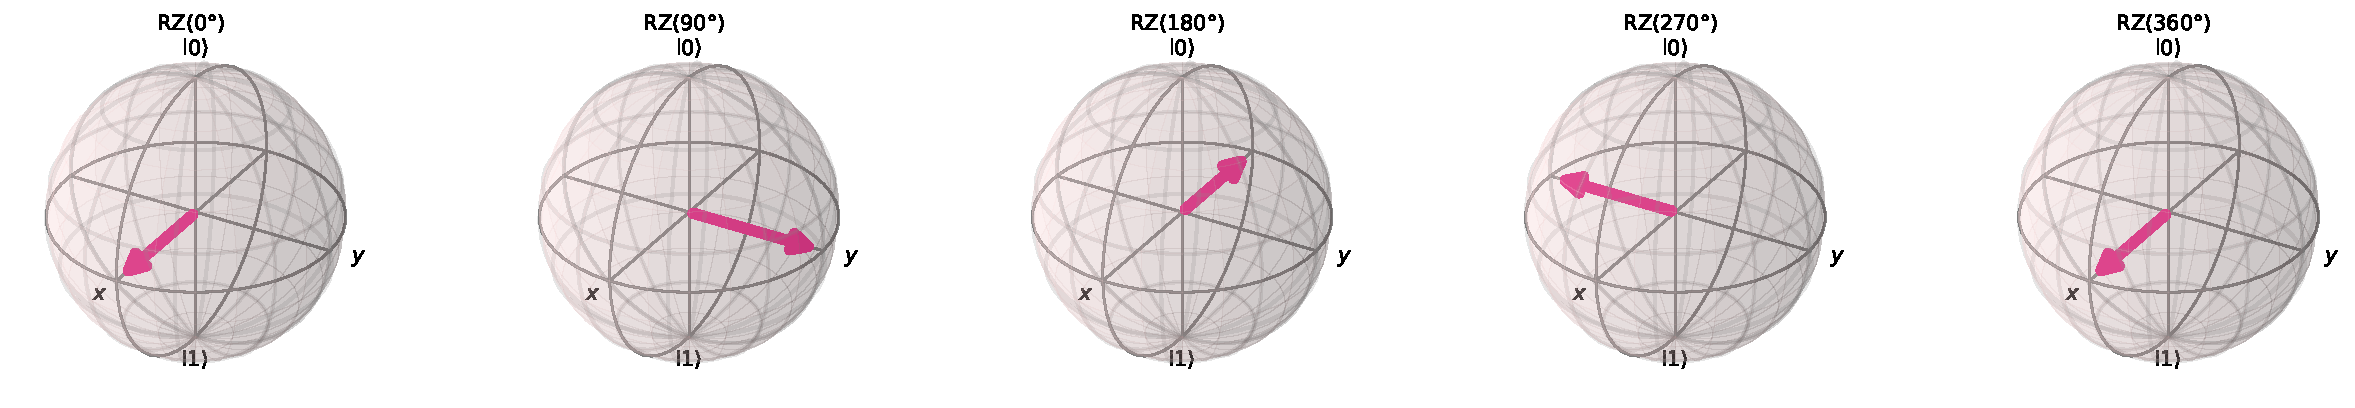
\includegraphics[keepaspectratio]{apostila_files/figure-pdf/cell-25-output-2.pdf}}

\begin{verbatim}

======================================================================
Observações importantes:
  • As PROBABILIDADES não mudam (sempre 50%-50%)
  • O qubit permanece no EQUADOR da esfera
  • Apenas a FASE (direção no equador) muda
  • RZ(0°) = |+⟩, RZ(180°) = |-⟩
======================================================================
\end{verbatim}

\begin{verbatim}
======================================================================
PORTA RZ: Rotação em torno do eixo Z (afeta apenas a fase)
======================================================================

Estado inicial: |+⟩ = H|0⟩
  |+⟩ = 0.7071+0.0000j|0⟩ + 0.7071+0.0000j|1⟩

0° (θ = 0.0000 rad):
  RZ(0.0000)|+⟩ = 0.7071+0.0000j|0⟩ + 0.7071+0.0000j|1⟩
  Fase de |1⟩: 0.00°
  Probabilidades: P(0) = 0.5000, P(1) = 0.5000

90° (θ = 1.5708 rad):
  RZ(1.5708)|+⟩ = 0.5000-0.5000j|0⟩ + 0.5000+0.5000j|1⟩
  Fase de |1⟩: 45.00°
  Probabilidades: P(0) = 0.5000, P(1) = 0.5000

180° (θ = 3.1416 rad):
  RZ(3.1416)|+⟩ = 0.0000-0.7071j|0⟩ + 0.0000+0.7071j|1⟩
  Fase de |1⟩: 90.00°
  Probabilidades: P(0) = 0.5000, P(1) = 0.5000

270° (θ = 4.7124 rad):
  RZ(4.7124)|+⟩ = -0.5000-0.5000j|0⟩ + -0.5000+0.5000j|1⟩
  Fase de |1⟩: 135.00°
  Probabilidades: P(0) = 0.5000, P(1) = 0.5000

360° (θ = 6.2832 rad):
  RZ(6.2832)|+⟩ = -0.7071-0.0000j|0⟩ + -0.7071+0.0000j|1⟩
  Fase de |1⟩: 180.00°
  Probabilidades: P(0) = 0.5000, P(1) = 0.5000
\end{verbatim}

\begin{verbatim}

======================================================================
Observações importantes:
  • As PROBABILIDADES não mudam (sempre 50%-50%)
  • O qubit permanece no EQUADOR da esfera
  • Apenas a FASE (direção no equador) muda
  • RZ(0°) = |+⟩, RZ(180°) = |-⟩
======================================================================
\end{verbatim}

\subsection{🔬 Exemplo 3: Porta RX - Completando o
trio}\label{exemplo-3-porta-rx---completando-o-trio}

A porta \textbf{RX(θ)} rotaciona em torno do eixo X. É menos comum que
RY e RZ, mas ainda importante para: - Criar estados em planos diferentes
da Esfera de Bloch - Algoritmos que precisam explorar todas as direções

Vamos ver RX em ação:

\begin{Shaded}
\begin{Highlighting}[]
\BuiltInTok{print}\NormalTok{(}\StringTok{"="} \OperatorTok{*} \DecValTok{70}\NormalTok{)}
\BuiltInTok{print}\NormalTok{(}\StringTok{"PORTA RX: Rotação em torno do eixo X"}\NormalTok{)}
\BuiltInTok{print}\NormalTok{(}\StringTok{"="} \OperatorTok{*} \DecValTok{70}\NormalTok{)}

\NormalTok{angulos\_rx }\OperatorTok{=}\NormalTok{ [}\DecValTok{0}\NormalTok{, np.pi}\OperatorTok{/}\DecValTok{2}\NormalTok{, np.pi, }\DecValTok{3}\OperatorTok{*}\NormalTok{np.pi}\OperatorTok{/}\DecValTok{2}\NormalTok{]}
\NormalTok{nomes\_rx }\OperatorTok{=}\NormalTok{ [}\StringTok{\textquotesingle{}0°\textquotesingle{}}\NormalTok{, }\StringTok{\textquotesingle{}90°\textquotesingle{}}\NormalTok{, }\StringTok{\textquotesingle{}180°\textquotesingle{}}\NormalTok{, }\StringTok{\textquotesingle{}270°\textquotesingle{}}\NormalTok{]}

\NormalTok{fig, axes }\OperatorTok{=}\NormalTok{ plt.subplots(}\DecValTok{1}\NormalTok{, }\DecValTok{4}\NormalTok{, figsize}\OperatorTok{=}\NormalTok{(}\DecValTok{16}\NormalTok{, }\DecValTok{4}\NormalTok{), subplot\_kw}\OperatorTok{=}\NormalTok{\{}\StringTok{\textquotesingle{}projection\textquotesingle{}}\NormalTok{: }\StringTok{\textquotesingle{}3d\textquotesingle{}}\NormalTok{\})}

\ControlFlowTok{for}\NormalTok{ i, (angulo, nome) }\KeywordTok{in} \BuiltInTok{enumerate}\NormalTok{(}\BuiltInTok{zip}\NormalTok{(angulos\_rx, nomes\_rx)):}
\NormalTok{    qc }\OperatorTok{=}\NormalTok{ QuantumCircuit(}\DecValTok{1}\NormalTok{)}
\NormalTok{    qc.rx(angulo, }\DecValTok{0}\NormalTok{)}
    
\NormalTok{    state }\OperatorTok{=}\NormalTok{ Statevector(qc)}
\NormalTok{    alpha }\OperatorTok{=}\NormalTok{ state.data[}\DecValTok{0}\NormalTok{]}
\NormalTok{    beta }\OperatorTok{=}\NormalTok{ state.data[}\DecValTok{1}\NormalTok{]}
    
    \BuiltInTok{print}\NormalTok{(}\SpecialStringTok{f"}\CharTok{\textbackslash{}n}\SpecialCharTok{\{}\NormalTok{nome}\SpecialCharTok{\}}\SpecialStringTok{ (θ = }\SpecialCharTok{\{}\NormalTok{angulo}\SpecialCharTok{:.4f\}}\SpecialStringTok{ rad):"}\NormalTok{)}
    \BuiltInTok{print}\NormalTok{(}\SpecialStringTok{f"  RX(}\SpecialCharTok{\{}\NormalTok{angulo}\SpecialCharTok{:.4f\}}\SpecialStringTok{)|0⟩ = }\SpecialCharTok{\{}\NormalTok{alpha}\SpecialCharTok{\}}\SpecialStringTok{|0⟩ + }\SpecialCharTok{\{}\NormalTok{beta}\SpecialCharTok{\}}\SpecialStringTok{|1⟩"}\NormalTok{)}
    \BuiltInTok{print}\NormalTok{(}\SpecialStringTok{f"  Probabilidades: P(0) = }\SpecialCharTok{\{}\BuiltInTok{abs}\NormalTok{(alpha)}\OperatorTok{**}\DecValTok{2}\SpecialCharTok{:.4f\}}\SpecialStringTok{, P(1) = }\SpecialCharTok{\{}\BuiltInTok{abs}\NormalTok{(beta)}\OperatorTok{**}\DecValTok{2}\SpecialCharTok{:.4f\}}\SpecialStringTok{"}\NormalTok{)}
    
    \CommentTok{\# Coordenadas de Bloch}
\NormalTok{    x }\OperatorTok{=} \DecValTok{2} \OperatorTok{*}\NormalTok{ (alpha.conjugate() }\OperatorTok{*}\NormalTok{ beta).real}
\NormalTok{    y }\OperatorTok{=} \DecValTok{2} \OperatorTok{*}\NormalTok{ (alpha.conjugate() }\OperatorTok{*}\NormalTok{ beta).imag}
\NormalTok{    z }\OperatorTok{=} \BuiltInTok{abs}\NormalTok{(alpha)}\OperatorTok{**}\DecValTok{2} \OperatorTok{{-}} \BuiltInTok{abs}\NormalTok{(beta)}\OperatorTok{**}\DecValTok{2}
    
\NormalTok{    plot\_bloch\_vector([x, y, z], ax}\OperatorTok{=}\NormalTok{axes[i], title}\OperatorTok{=}\SpecialStringTok{f\textquotesingle{}RX(}\SpecialCharTok{\{}\NormalTok{nome}\SpecialCharTok{\}}\SpecialStringTok{)\textquotesingle{}}\NormalTok{)}

\NormalTok{plt.subplots\_adjust(wspace}\OperatorTok{=}\FloatTok{0.4}\NormalTok{)}
\NormalTok{plt.show()}

\BuiltInTok{print}\NormalTok{(}\StringTok{"}\CharTok{\textbackslash{}n}\StringTok{"} \OperatorTok{+} \StringTok{"="} \OperatorTok{*} \DecValTok{70}\NormalTok{)}
\BuiltInTok{print}\NormalTok{(}\StringTok{"Observações:"}\NormalTok{)}
\BuiltInTok{print}\NormalTok{(}\StringTok{"  • RX rotaciona no plano YZ"}\NormalTok{)}
\BuiltInTok{print}\NormalTok{(}\StringTok{"  • RX(90°) cria superposição com números complexos"}\NormalTok{)}
\BuiltInTok{print}\NormalTok{(}\StringTok{"  • RX(180°) = X (porta NOT)"}\NormalTok{)}
\BuiltInTok{print}\NormalTok{(}\StringTok{"="} \OperatorTok{*} \DecValTok{70}\NormalTok{)}
\end{Highlighting}
\end{Shaded}

\begin{verbatim}
======================================================================
PORTA RX: Rotação em torno do eixo X
======================================================================

0° (θ = 0.0000 rad):
  RX(0.0000)|0⟩ = (1+0j)|0⟩ + 0j|1⟩
  Probabilidades: P(0) = 1.0000, P(1) = 0.0000

90° (θ = 1.5708 rad):
  RX(1.5708)|0⟩ = (0.7071067811865476+0j)|0⟩ + -0.7071067811865475j|1⟩
  Probabilidades: P(0) = 0.5000, P(1) = 0.5000

180° (θ = 3.1416 rad):
  RX(3.1416)|0⟩ = (6.123233995736766e-17+0j)|0⟩ + -1j|1⟩
  Probabilidades: P(0) = 0.0000, P(1) = 1.0000

270° (θ = 4.7124 rad):
  RX(4.7124)|0⟩ = (-0.7071067811865475+0j)|0⟩ + -0.7071067811865476j|1⟩
  Probabilidades: P(0) = 0.5000, P(1) = 0.5000
\end{verbatim}

\pandocbounded{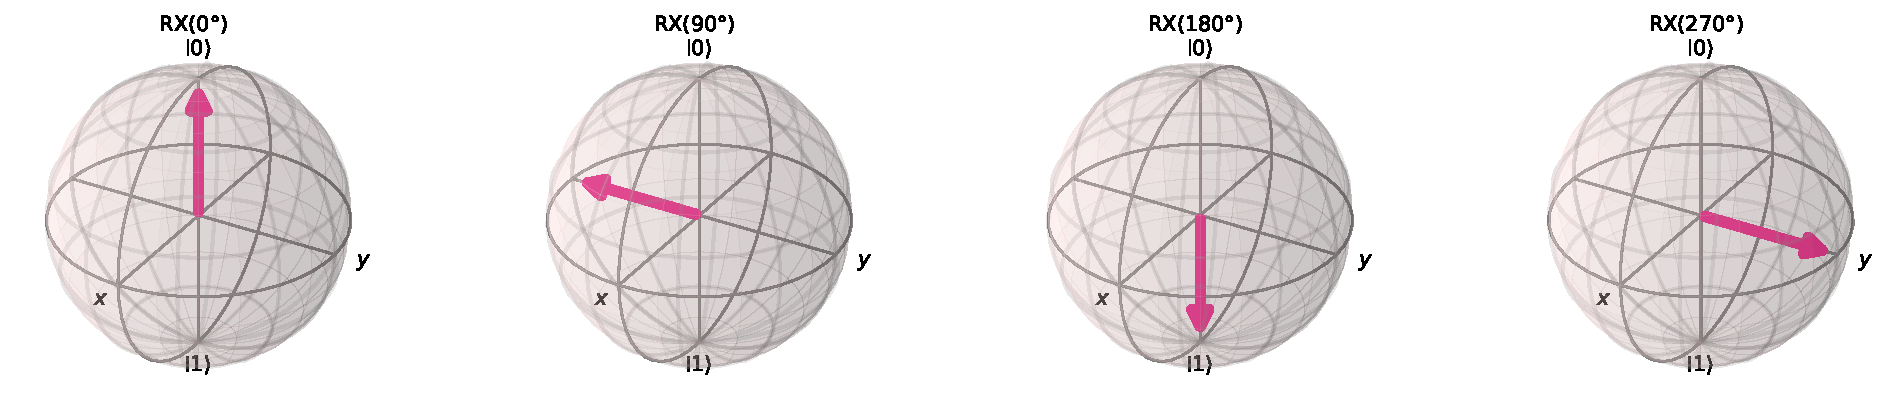
\includegraphics[keepaspectratio]{apostila_files/figure-pdf/cell-26-output-2.pdf}}

\begin{verbatim}

======================================================================
Observações:
  • RX rotaciona no plano YZ
  • RX(90°) cria superposição com números complexos
  • RX(180°) = X (porta NOT)
======================================================================
\end{verbatim}

\begin{verbatim}
======================================================================
PORTA RX: Rotação em torno do eixo X
======================================================================

0° (θ = 0.0000 rad):
  RX(0.0000)|0⟩ = (1+0j)|0⟩ + 0j|1⟩
  Probabilidades: P(0) = 1.0000, P(1) = 0.0000

90° (θ = 1.5708 rad):
  RX(1.5708)|0⟩ = (0.7071067811865476+0j)|0⟩ + -0.7071067811865476j|1⟩
  Probabilidades: P(0) = 0.5000, P(1) = 0.5000

180° (θ = 3.1416 rad):
  RX(3.1416)|0⟩ = (6.123233995736766e-17+0j)|0⟩ + -1j|1⟩
  Probabilidades: P(0) = 0.0000, P(1) = 1.0000

270° (θ = 4.7124 rad):
  RX(4.7124)|0⟩ = (-0.7071067811865475+0j)|0⟩ + -0.7071067811865476j|1⟩
  Probabilidades: P(0) = 0.5000, P(1) = 0.5000
\end{verbatim}

\begin{verbatim}

======================================================================
Observações:
  • RX rotaciona no plano YZ
  • RX(90°) cria superposição com números complexos
  • RX(180°) = X (porta NOT)
======================================================================
\end{verbatim}

\subsection{🛠️ Implementação Manual das Portas de
Rotação}\label{implementauxe7uxe3o-manual-das-portas-de-rotauxe7uxe3o}

Vamos implementar as portas de rotação usando apenas NumPy. Isso ajuda a
entender como elas realmente funcionam ``por baixo dos panos'':

\textbf{Lembre-se:} As matrizes usam \textbf{θ/2} (metade do ângulo),
então para uma rotação de 90° na Esfera de Bloch, passamos θ = π/2 rad
(45° nas matrizes).

\begin{Shaded}
\begin{Highlighting}[]
\ImportTok{import}\NormalTok{ numpy }\ImportTok{as}\NormalTok{ np}

\CommentTok{\# Implementação manual das portas de rotação parametrizadas}
\KeywordTok{def}\NormalTok{ rx\_gate(theta):}
    \CommentTok{"""Porta RX(θ) {-} Rotação em torno do eixo X"""}
    \ControlFlowTok{return}\NormalTok{ np.array([}
\NormalTok{        [np.cos(theta}\OperatorTok{/}\DecValTok{2}\NormalTok{), }\OperatorTok{{-}}\OtherTok{1j}\OperatorTok{*}\NormalTok{np.sin(theta}\OperatorTok{/}\DecValTok{2}\NormalTok{)],}
\NormalTok{        [}\OperatorTok{{-}}\OtherTok{1j}\OperatorTok{*}\NormalTok{np.sin(theta}\OperatorTok{/}\DecValTok{2}\NormalTok{), np.cos(theta}\OperatorTok{/}\DecValTok{2}\NormalTok{)]}
\NormalTok{    ])}

\KeywordTok{def}\NormalTok{ ry\_gate(theta):}
    \CommentTok{"""Porta RY(θ) {-} Rotação em torno do eixo Y"""}
    \ControlFlowTok{return}\NormalTok{ np.array([}
\NormalTok{        [np.cos(theta}\OperatorTok{/}\DecValTok{2}\NormalTok{), }\OperatorTok{{-}}\NormalTok{np.sin(theta}\OperatorTok{/}\DecValTok{2}\NormalTok{)],}
\NormalTok{        [np.sin(theta}\OperatorTok{/}\DecValTok{2}\NormalTok{), np.cos(theta}\OperatorTok{/}\DecValTok{2}\NormalTok{)]}
\NormalTok{    ])}

\KeywordTok{def}\NormalTok{ rz\_gate(theta):}
    \CommentTok{"""Porta RZ(θ) {-} Rotação em torno do eixo Z"""}
    \ControlFlowTok{return}\NormalTok{ np.array([}
\NormalTok{        [np.exp(}\OperatorTok{{-}}\OtherTok{1j}\OperatorTok{*}\NormalTok{theta}\OperatorTok{/}\DecValTok{2}\NormalTok{), }\DecValTok{0}\NormalTok{],}
\NormalTok{        [}\DecValTok{0}\NormalTok{, np.exp(}\OtherTok{1j}\OperatorTok{*}\NormalTok{theta}\OperatorTok{/}\DecValTok{2}\NormalTok{)]}
\NormalTok{    ])}

\CommentTok{\# Estados básicos}
\NormalTok{ket\_0 }\OperatorTok{=}\NormalTok{ np.array([[}\DecValTok{1}\NormalTok{], [}\DecValTok{0}\NormalTok{]])}
\NormalTok{ket\_1 }\OperatorTok{=}\NormalTok{ np.array([[}\DecValTok{0}\NormalTok{], [}\DecValTok{1}\NormalTok{]])}

\BuiltInTok{print}\NormalTok{(}\StringTok{"="} \OperatorTok{*} \DecValTok{70}\NormalTok{)}
\BuiltInTok{print}\NormalTok{(}\StringTok{"IMPLEMENTAÇÃO MANUAL DAS PORTAS DE ROTAÇÃO"}\NormalTok{)}
\BuiltInTok{print}\NormalTok{(}\StringTok{"="} \OperatorTok{*} \DecValTok{70}\NormalTok{)}

\CommentTok{\# Testar RY com θ = π/2 (90° na Esfera de Bloch)}
\NormalTok{theta }\OperatorTok{=}\NormalTok{ np.pi }\OperatorTok{/} \DecValTok{2}
\BuiltInTok{print}\NormalTok{(}\SpecialStringTok{f"}\CharTok{\textbackslash{}n}\SpecialStringTok{🔹 Testando RY(}\SpecialCharTok{\{}\NormalTok{theta}\SpecialCharTok{:.4f\}}\SpecialStringTok{) em |0⟩:"}\NormalTok{)}
\BuiltInTok{print}\NormalTok{(}\SpecialStringTok{f"   Ângulo: π/2 = 90° na Esfera de Bloch"}\NormalTok{)}

\NormalTok{RY }\OperatorTok{=}\NormalTok{ ry\_gate(theta)}
\NormalTok{state\_ry }\OperatorTok{=}\NormalTok{ RY.dot(ket\_0)}

\BuiltInTok{print}\NormalTok{(}\SpecialStringTok{f"}\CharTok{\textbackslash{}n}\SpecialStringTok{   Matriz RY(π/2):"}\NormalTok{)}
\BuiltInTok{print}\NormalTok{(}\SpecialStringTok{f"   }\SpecialCharTok{\{}\NormalTok{RY[}\DecValTok{0}\NormalTok{]}\SpecialCharTok{\}}\SpecialStringTok{"}\NormalTok{)}
\BuiltInTok{print}\NormalTok{(}\SpecialStringTok{f"   }\SpecialCharTok{\{}\NormalTok{RY[}\DecValTok{1}\NormalTok{]}\SpecialCharTok{\}}\SpecialStringTok{"}\NormalTok{)}

\BuiltInTok{print}\NormalTok{(}\SpecialStringTok{f"}\CharTok{\textbackslash{}n}\SpecialStringTok{   RY(π/2)|0⟩ = }\SpecialCharTok{\{}\NormalTok{state\_ry[}\DecValTok{0}\NormalTok{][}\DecValTok{0}\NormalTok{]}\SpecialCharTok{:.4f\}}\SpecialStringTok{|0⟩ + }\SpecialCharTok{\{}\NormalTok{state\_ry[}\DecValTok{1}\NormalTok{][}\DecValTok{0}\NormalTok{]}\SpecialCharTok{:.4f\}}\SpecialStringTok{|1⟩"}\NormalTok{)}
\BuiltInTok{print}\NormalTok{(}\SpecialStringTok{f"   Esperado: 1/√2|0⟩ + 1/√2|1⟩ = |+⟩"}\NormalTok{)}
\BuiltInTok{print}\NormalTok{(}\SpecialStringTok{f"   Probabilidades: P(0) = }\SpecialCharTok{\{}\BuiltInTok{abs}\NormalTok{(state\_ry[}\DecValTok{0}\NormalTok{][}\DecValTok{0}\NormalTok{])}\OperatorTok{**}\DecValTok{2}\SpecialCharTok{:.4f\}}\SpecialStringTok{, P(1) = }\SpecialCharTok{\{}\BuiltInTok{abs}\NormalTok{(state\_ry[}\DecValTok{1}\NormalTok{][}\DecValTok{0}\NormalTok{])}\OperatorTok{**}\DecValTok{2}\SpecialCharTok{:.4f\}}\SpecialStringTok{"}\NormalTok{)}

\CommentTok{\# Testar RZ com θ = π (180°)}
\BuiltInTok{print}\NormalTok{(}\SpecialStringTok{f"}\CharTok{\textbackslash{}n}\SpecialStringTok{🔹 Testando RZ(π) aplicado a |+⟩:"}\NormalTok{)}
\BuiltInTok{print}\NormalTok{(}\SpecialStringTok{f"   Ângulo: π = 180° na Esfera de Bloch"}\NormalTok{)}

\CommentTok{\# Primeiro criar |+⟩}
\NormalTok{H }\OperatorTok{=} \DecValTok{1}\OperatorTok{/}\NormalTok{np.sqrt(}\DecValTok{2}\NormalTok{) }\OperatorTok{*}\NormalTok{ np.array([[}\DecValTok{1}\NormalTok{, }\DecValTok{1}\NormalTok{], [}\DecValTok{1}\NormalTok{, }\OperatorTok{{-}}\DecValTok{1}\NormalTok{]])  }\CommentTok{\# Porta Hadamard}
\NormalTok{ket\_plus }\OperatorTok{=}\NormalTok{ H.dot(ket\_0)}

\NormalTok{RZ }\OperatorTok{=}\NormalTok{ rz\_gate(np.pi)}
\NormalTok{state\_rz }\OperatorTok{=}\NormalTok{ RZ.dot(ket\_plus.reshape(}\DecValTok{2}\NormalTok{,}\DecValTok{1}\NormalTok{))}

\BuiltInTok{print}\NormalTok{(}\SpecialStringTok{f"}\CharTok{\textbackslash{}n}\SpecialStringTok{   Estado inicial: |+⟩ = }\SpecialCharTok{\{}\NormalTok{ket\_plus[}\DecValTok{0}\NormalTok{][}\DecValTok{0}\NormalTok{]}\SpecialCharTok{:.4f\}}\SpecialStringTok{|0⟩ + }\SpecialCharTok{\{}\NormalTok{ket\_plus[}\DecValTok{1}\NormalTok{][}\DecValTok{0}\NormalTok{]}\SpecialCharTok{:.4f\}}\SpecialStringTok{|1⟩"}\NormalTok{)}
\BuiltInTok{print}\NormalTok{(}\SpecialStringTok{f"}\CharTok{\textbackslash{}n}\SpecialStringTok{   Matriz RZ(π):"}\NormalTok{)}
\BuiltInTok{print}\NormalTok{(}\SpecialStringTok{f"   }\SpecialCharTok{\{}\NormalTok{RZ[}\DecValTok{0}\NormalTok{]}\SpecialCharTok{\}}\SpecialStringTok{"}\NormalTok{)}
\BuiltInTok{print}\NormalTok{(}\SpecialStringTok{f"   }\SpecialCharTok{\{}\NormalTok{RZ[}\DecValTok{1}\NormalTok{]}\SpecialCharTok{\}}\SpecialStringTok{"}\NormalTok{)}

\CommentTok{\# Simplificar a fase global e\^{}({-}iπ/2) = {-}i}
\NormalTok{phase\_global }\OperatorTok{=}\NormalTok{ np.exp(}\OperatorTok{{-}}\OtherTok{1j}\OperatorTok{*}\NormalTok{np.pi}\OperatorTok{/}\DecValTok{2}\NormalTok{)}
\NormalTok{state\_rz\_simplified }\OperatorTok{=}\NormalTok{ state\_rz }\OperatorTok{/}\NormalTok{ phase\_global}

\BuiltInTok{print}\NormalTok{(}\SpecialStringTok{f"}\CharTok{\textbackslash{}n}\SpecialStringTok{   RZ(π)|+⟩ = }\SpecialCharTok{\{}\NormalTok{state\_rz[}\DecValTok{0}\NormalTok{][}\DecValTok{0}\NormalTok{]}\SpecialCharTok{:.4f\}}\SpecialStringTok{|0⟩ + }\SpecialCharTok{\{}\NormalTok{state\_rz[}\DecValTok{1}\NormalTok{][}\DecValTok{0}\NormalTok{]}\SpecialCharTok{:.4f\}}\SpecialStringTok{|1⟩"}\NormalTok{)}
\BuiltInTok{print}\NormalTok{(}\SpecialStringTok{f"   Removendo fase global: ≈ }\SpecialCharTok{\{}\NormalTok{state\_rz\_simplified[}\DecValTok{0}\NormalTok{][}\DecValTok{0}\NormalTok{]}\SpecialCharTok{:.4f\}}\SpecialStringTok{|0⟩ + }\SpecialCharTok{\{}\NormalTok{state\_rz\_simplified[}\DecValTok{1}\NormalTok{][}\DecValTok{0}\NormalTok{]}\SpecialCharTok{:.4f\}}\SpecialStringTok{|1⟩"}\NormalTok{)}
\BuiltInTok{print}\NormalTok{(}\SpecialStringTok{f"   Esperado: 1/√2|0⟩ {-} 1/√2|1⟩ = |{-}⟩"}\NormalTok{)}
\BuiltInTok{print}\NormalTok{(}\SpecialStringTok{f"   ✅ RZ(π) = Z (porta Z é caso especial de RZ)"}\NormalTok{)}

\CommentTok{\# Testar RX com θ = π (180° = porta X)}
\BuiltInTok{print}\NormalTok{(}\SpecialStringTok{f"}\CharTok{\textbackslash{}n}\SpecialStringTok{🔹 Testando RX(π) em |0⟩:"}\NormalTok{)}
\BuiltInTok{print}\NormalTok{(}\SpecialStringTok{f"   Ângulo: π = 180° na Esfera de Bloch"}\NormalTok{)}

\NormalTok{RX }\OperatorTok{=}\NormalTok{ rx\_gate(np.pi)}
\NormalTok{state\_rx }\OperatorTok{=}\NormalTok{ RX.dot(ket\_0)}

\CommentTok{\# Remover fase global {-}i}
\NormalTok{state\_rx\_real }\OperatorTok{=}\NormalTok{ state\_rx }\OperatorTok{/}\NormalTok{ (}\OperatorTok{{-}}\OtherTok{1j}\NormalTok{)}

\BuiltInTok{print}\NormalTok{(}\SpecialStringTok{f"}\CharTok{\textbackslash{}n}\SpecialStringTok{   Matriz RX(π):"}\NormalTok{)}
\BuiltInTok{print}\NormalTok{(}\SpecialStringTok{f"   }\SpecialCharTok{\{}\NormalTok{RX[}\DecValTok{0}\NormalTok{]}\SpecialCharTok{\}}\SpecialStringTok{"}\NormalTok{)}
\BuiltInTok{print}\NormalTok{(}\SpecialStringTok{f"   }\SpecialCharTok{\{}\NormalTok{RX[}\DecValTok{1}\NormalTok{]}\SpecialCharTok{\}}\SpecialStringTok{"}\NormalTok{)}

\BuiltInTok{print}\NormalTok{(}\SpecialStringTok{f"}\CharTok{\textbackslash{}n}\SpecialStringTok{   RX(π)|0⟩ = }\SpecialCharTok{\{}\NormalTok{state\_rx[}\DecValTok{0}\NormalTok{][}\DecValTok{0}\NormalTok{]}\SpecialCharTok{\}}\SpecialStringTok{|0⟩ + }\SpecialCharTok{\{}\NormalTok{state\_rx[}\DecValTok{1}\NormalTok{][}\DecValTok{0}\NormalTok{]}\SpecialCharTok{\}}\SpecialStringTok{|1⟩"}\NormalTok{)}
\BuiltInTok{print}\NormalTok{(}\SpecialStringTok{f"   Removendo fase global: ≈ }\SpecialCharTok{\{}\NormalTok{state\_rx\_real[}\DecValTok{0}\NormalTok{][}\DecValTok{0}\NormalTok{]}\SpecialCharTok{:.4f\}}\SpecialStringTok{|0⟩ + }\SpecialCharTok{\{}\NormalTok{state\_rx\_real[}\DecValTok{1}\NormalTok{][}\DecValTok{0}\NormalTok{]}\SpecialCharTok{:.4f\}}\SpecialStringTok{|1⟩"}\NormalTok{)}
\BuiltInTok{print}\NormalTok{(}\SpecialStringTok{f"   Esperado: |1⟩"}\NormalTok{)}
\BuiltInTok{print}\NormalTok{(}\SpecialStringTok{f"   ✅ RX(π) = X (porta X é caso especial de RX)"}\NormalTok{)}

\CommentTok{\# Verificar casos especiais}
\BuiltInTok{print}\NormalTok{(}\StringTok{"}\CharTok{\textbackslash{}n}\StringTok{"} \OperatorTok{+} \StringTok{"="} \OperatorTok{*} \DecValTok{70}\NormalTok{)}
\BuiltInTok{print}\NormalTok{(}\StringTok{"CASOS ESPECIAIS (relação com portas fixas):"}\NormalTok{)}
\BuiltInTok{print}\NormalTok{(}\StringTok{"="} \OperatorTok{*} \DecValTok{70}\NormalTok{)}

\CommentTok{\# Porta Z}
\NormalTok{Z }\OperatorTok{=}\NormalTok{ np.array([[}\DecValTok{1}\NormalTok{, }\DecValTok{0}\NormalTok{], [}\DecValTok{0}\NormalTok{, }\OperatorTok{{-}}\DecValTok{1}\NormalTok{]])}
\NormalTok{RZ\_pi }\OperatorTok{=}\NormalTok{ rz\_gate(np.pi)}
\CommentTok{\# Remover fase global}
\NormalTok{RZ\_pi\_simplified }\OperatorTok{=}\NormalTok{ RZ\_pi }\OperatorTok{/}\NormalTok{ np.exp(}\OperatorTok{{-}}\OtherTok{1j}\OperatorTok{*}\NormalTok{np.pi}\OperatorTok{/}\DecValTok{2}\NormalTok{)}
\BuiltInTok{print}\NormalTok{(}\SpecialStringTok{f"}\CharTok{\textbackslash{}n}\SpecialStringTok{Z vs RZ(π):"}\NormalTok{)}
\BuiltInTok{print}\NormalTok{(}\SpecialStringTok{f"  Z =     }\SpecialCharTok{\{}\NormalTok{Z[}\DecValTok{0}\NormalTok{]}\SpecialCharTok{\}}\SpecialStringTok{  }\SpecialCharTok{\{}\NormalTok{Z[}\DecValTok{1}\NormalTok{]}\SpecialCharTok{\}}\SpecialStringTok{"}\NormalTok{)}
\BuiltInTok{print}\NormalTok{(}\SpecialStringTok{f"  RZ(π) = }\SpecialCharTok{\{}\NormalTok{RZ\_pi\_simplified[}\DecValTok{0}\NormalTok{]}\SpecialCharTok{\}}\SpecialStringTok{  }\SpecialCharTok{\{}\NormalTok{RZ\_pi\_simplified[}\DecValTok{1}\NormalTok{]}\SpecialCharTok{\}}\SpecialStringTok{"}\NormalTok{)}
\BuiltInTok{print}\NormalTok{(}\SpecialStringTok{f"  ✅ Equivalentes (a menos de fase global)"}\NormalTok{)}

\CommentTok{\# Porta S}
\NormalTok{S }\OperatorTok{=}\NormalTok{ np.array([[}\DecValTok{1}\NormalTok{, }\DecValTok{0}\NormalTok{], [}\DecValTok{0}\NormalTok{, }\OtherTok{1j}\NormalTok{]])}
\NormalTok{RZ\_pi\_2 }\OperatorTok{=}\NormalTok{ rz\_gate(np.pi}\OperatorTok{/}\DecValTok{2}\NormalTok{)}
\CommentTok{\# Remover fase global}
\NormalTok{RZ\_pi\_2\_simplified }\OperatorTok{=}\NormalTok{ RZ\_pi\_2 }\OperatorTok{/}\NormalTok{ np.exp(}\OperatorTok{{-}}\OtherTok{1j}\OperatorTok{*}\NormalTok{np.pi}\OperatorTok{/}\DecValTok{4}\NormalTok{)}
\BuiltInTok{print}\NormalTok{(}\SpecialStringTok{f"}\CharTok{\textbackslash{}n}\SpecialStringTok{S vs RZ(π/2):"}\NormalTok{)}
\BuiltInTok{print}\NormalTok{(}\SpecialStringTok{f"  S =       }\SpecialCharTok{\{}\NormalTok{S[}\DecValTok{0}\NormalTok{]}\SpecialCharTok{\}}\SpecialStringTok{  }\SpecialCharTok{\{}\NormalTok{S[}\DecValTok{1}\NormalTok{]}\SpecialCharTok{\}}\SpecialStringTok{"}\NormalTok{)}
\BuiltInTok{print}\NormalTok{(}\SpecialStringTok{f"  RZ(π/2) = }\SpecialCharTok{\{}\NormalTok{RZ\_pi\_2\_simplified[}\DecValTok{0}\NormalTok{]}\SpecialCharTok{\}}\SpecialStringTok{  }\SpecialCharTok{\{}\NormalTok{RZ\_pi\_2\_simplified[}\DecValTok{1}\NormalTok{]}\SpecialCharTok{\}}\SpecialStringTok{"}\NormalTok{)}
\BuiltInTok{print}\NormalTok{(}\SpecialStringTok{f"  ✅ Equivalentes (a menos de fase global)"}\NormalTok{)}

\CommentTok{\# Porta X}
\NormalTok{X }\OperatorTok{=}\NormalTok{ np.array([[}\DecValTok{0}\NormalTok{, }\DecValTok{1}\NormalTok{], [}\DecValTok{1}\NormalTok{, }\DecValTok{0}\NormalTok{]])}
\NormalTok{RX\_pi }\OperatorTok{=}\NormalTok{ rx\_gate(np.pi)}
\NormalTok{RX\_pi\_simplified }\OperatorTok{=}\NormalTok{ RX\_pi }\OperatorTok{/}\NormalTok{ (}\OperatorTok{{-}}\OtherTok{1j}\NormalTok{)}
\BuiltInTok{print}\NormalTok{(}\SpecialStringTok{f"}\CharTok{\textbackslash{}n}\SpecialStringTok{X vs RX(π):"}\NormalTok{)}
\BuiltInTok{print}\NormalTok{(}\SpecialStringTok{f"  X =     }\SpecialCharTok{\{}\NormalTok{X[}\DecValTok{0}\NormalTok{]}\SpecialCharTok{\}}\SpecialStringTok{  }\SpecialCharTok{\{}\NormalTok{X[}\DecValTok{1}\NormalTok{]}\SpecialCharTok{\}}\SpecialStringTok{"}\NormalTok{)}
\BuiltInTok{print}\NormalTok{(}\SpecialStringTok{f"  RX(π) = }\SpecialCharTok{\{}\NormalTok{RX\_pi\_simplified[}\DecValTok{0}\NormalTok{]}\SpecialCharTok{\}}\SpecialStringTok{  }\SpecialCharTok{\{}\NormalTok{RX\_pi\_simplified[}\DecValTok{1}\NormalTok{]}\SpecialCharTok{\}}\SpecialStringTok{"}\NormalTok{)}
\BuiltInTok{print}\NormalTok{(}\SpecialStringTok{f"  ✅ Equivalentes (a menos de fase global)"}\NormalTok{)}

\BuiltInTok{print}\NormalTok{(}\StringTok{"}\CharTok{\textbackslash{}n}\StringTok{"} \OperatorTok{+} \StringTok{"="} \OperatorTok{*} \DecValTok{70}\NormalTok{)}
\BuiltInTok{print}\NormalTok{(}\StringTok{"💡 CONCLUSÃO:"}\NormalTok{)}
\BuiltInTok{print}\NormalTok{(}\StringTok{"   As portas fixas (X, Z, S, T) são casos especiais das portas"}\NormalTok{)}
\BuiltInTok{print}\NormalTok{(}\StringTok{"   de rotação parametrizadas com ângulos específicos!"}\NormalTok{)}
\BuiltInTok{print}\NormalTok{(}\StringTok{"="} \OperatorTok{*} \DecValTok{70}\NormalTok{)}
\end{Highlighting}
\end{Shaded}

\begin{verbatim}
======================================================================
IMPLEMENTAÇÃO MANUAL DAS PORTAS DE ROTAÇÃO
======================================================================

🔹 Testando RY(1.5708) em |0⟩:
   Ângulo: π/2 = 90° na Esfera de Bloch

   Matriz RY(π/2):
   [ 0.70710678 -0.70710678]
   [0.70710678 0.70710678]

   RY(π/2)|0⟩ = 0.7071|0⟩ + 0.7071|1⟩
   Esperado: 1/√2|0⟩ + 1/√2|1⟩ = |+⟩
   Probabilidades: P(0) = 0.5000, P(1) = 0.5000

🔹 Testando RZ(π) aplicado a |+⟩:
   Ângulo: π = 180° na Esfera de Bloch

   Estado inicial: |+⟩ = 0.7071|0⟩ + 0.7071|1⟩

   Matriz RZ(π):
   [6.123234e-17-1.j 0.000000e+00+0.j]
   [0.000000e+00+0.j 6.123234e-17+1.j]

   RZ(π)|+⟩ = 0.0000-0.7071j|0⟩ + 0.0000+0.7071j|1⟩
   Removendo fase global: ≈ 0.7071-0.0000j|0⟩ + -0.7071+0.0000j|1⟩
   Esperado: 1/√2|0⟩ - 1/√2|1⟩ = |-⟩
   ✅ RZ(π) = Z (porta Z é caso especial de RZ)

🔹 Testando RX(π) em |0⟩:
   Ângulo: π = 180° na Esfera de Bloch

   Matriz RX(π):
   [6.123234e-17+0.j 0.000000e+00-1.j]
   [0.000000e+00-1.j 6.123234e-17+0.j]

   RX(π)|0⟩ = (6.123233995736766e-17+0j)|0⟩ + -1j|1⟩
   Removendo fase global: ≈ -0.0000+0.0000j|0⟩ + 1.0000+0.0000j|1⟩
   Esperado: |1⟩
   ✅ RX(π) = X (porta X é caso especial de RX)

======================================================================
CASOS ESPECIAIS (relação com portas fixas):
======================================================================

Z vs RZ(π):
  Z =     [1 0]  [ 0 -1]
  RZ(π) = [ 1.-0.j -0.+0.j]  [-0.+0.0000000e+00j -1.+1.2246468e-16j]
  ✅ Equivalentes (a menos de fase global)

S vs RZ(π/2):
  S =       [1.+0.j 0.+0.j]  [0.+0.j 0.+1.j]
  RZ(π/2) = [1.+0.j 0.+0.j]  [0.00000000e+00+0.j 1.57009246e-16+1.j]
  ✅ Equivalentes (a menos de fase global)

X vs RX(π):
  X =     [0 1]  [1 0]
  RX(π) = [-0.+6.123234e-17j  1.+0.000000e+00j]  [ 1.+0.000000e+00j -0.+6.123234e-17j]
  ✅ Equivalentes (a menos de fase global)

======================================================================
💡 CONCLUSÃO:
   As portas fixas (X, Z, S, T) são casos especiais das portas
   de rotação parametrizadas com ângulos específicos!
======================================================================
\end{verbatim}

\begin{verbatim}
======================================================================
IMPLEMENTAÇÃO MANUAL DAS PORTAS DE ROTAÇÃO
======================================================================

🔹 Testando RY(1.5708) em |0⟩:
   Ângulo: π/2 = 90° na Esfera de Bloch

   Matriz RY(π/2):
   [ 0.70710678 -0.70710678]
   [0.70710678 0.70710678]

   RY(π/2)|0⟩ = 0.7071|0⟩ + 0.7071|1⟩
   Esperado: 1/√2|0⟩ + 1/√2|1⟩ = |+⟩
   Probabilidades: P(0) = 0.5000, P(1) = 0.5000

🔹 Testando RZ(π) aplicado a |+⟩:
   Ângulo: π = 180° na Esfera de Bloch

   Estado inicial: |+⟩ = 0.7071|0⟩ + 0.7071|1⟩

   Matriz RZ(π):
   [6.123234e-17-1.j 0.000000e+00+0.j]
   [0.000000e+00+0.j 6.123234e-17+1.j]

   RZ(π)|+⟩ = 0.0000-0.7071j|0⟩ + 0.0000+0.7071j|1⟩
   Removendo fase global: ≈ 0.7071-0.0000j|0⟩ + -0.7071+0.0000j|1⟩
   Esperado: 1/√2|0⟩ - 1/√2|1⟩ = |-⟩
   ✅ RZ(π) = Z (porta Z é caso especial de RZ)

🔹 Testando RX(π) em |0⟩:
   Ângulo: π = 180° na Esfera de Bloch

   Matriz RX(π):
   [ 6.123234e-17+0.j -0.000000e+00-1.j]
   [-0.000000e+00-1.j  6.123234e-17+0.j]

   RX(π)|0⟩ = (6.123233995736766e-17+0j)|0⟩ + -1j|1⟩
   Removendo fase global: ≈ -0.0000+0.0000j|0⟩ + 1.0000+0.0000j|1⟩
   Esperado: |1⟩
   ✅ RX(π) = X (porta X é caso especial de RX)

======================================================================
CASOS ESPECIAIS (relação com portas fixas):
======================================================================

Z vs RZ(π):
  Z =     [1 0]  [ 0 -1]
  RZ(π) = [ 1.-0.j -0.+0.j]  [-0.+0.0000000e+00j -1.+1.2246468e-16j]
  ✅ Equivalentes (a menos de fase global)

S vs RZ(π/2):
  S =       [1.+0.j 0.+0.j]  [0.+0.j 0.+1.j]
  RZ(π/2) = [1.+0.j 0.+0.j]  [0.+0.j 0.+1.j]
  ✅ Equivalentes (a menos de fase global)

X vs RX(π):
  X =     [0 1]  [1 0]
  RX(π) = [-0.+6.123234e-17j  1.-0.000000e+00j]  [ 1.-0.000000e+00j -0.+6.123234e-17j]
  ✅ Equivalentes (a menos de fase global)

======================================================================
💡 CONCLUSÃO:
   As portas fixas (X, Z, S, T) são casos especiais das portas
   de rotação parametrizadas com ângulos específicos!
======================================================================
\end{verbatim}

\subsection{🎯 Aplicação Prática: Codificação de Dados
Clássicos}\label{aplicauxe7uxe3o-pruxe1tica-codificauxe7uxe3o-de-dados-cluxe1ssicos}

Uma das aplicações mais importantes de RY e RZ é \textbf{codificar dados
clássicos em estados quânticos}. Vamos ver um exemplo simples:

Suponha que você tem um dado clássico \texttt{x\ =\ 0.5} (normalizado
entre 0 e 1) e quer codificá-lo em um qubit. Você pode usar:

\begin{Shaded}
\begin{Highlighting}[]
\NormalTok{theta }\OperatorTok{=} \DecValTok{2} \OperatorTok{*}\NormalTok{ np.pi }\OperatorTok{*}\NormalTok{ x  }\CommentTok{\# Mapear [0,1] → [0, 2π]}
\NormalTok{qc.ry(theta, }\DecValTok{0}\NormalTok{)        }\CommentTok{\# Aplicar rotação RY}
\end{Highlighting}
\end{Shaded}

Vamos testar com diferentes valores:

\begin{Shaded}
\begin{Highlighting}[]
\CommentTok{\# Importações necessárias para esta célula}
\ImportTok{from}\NormalTok{ qiskit }\ImportTok{import}\NormalTok{ QuantumCircuit}
\ImportTok{from}\NormalTok{ qiskit.quantum\_info }\ImportTok{import}\NormalTok{ Statevector}
\ImportTok{from}\NormalTok{ qiskit.visualization }\ImportTok{import}\NormalTok{ plot\_bloch\_vector}
\ImportTok{import}\NormalTok{ matplotlib.pyplot }\ImportTok{as}\NormalTok{ plt}
\ImportTok{import}\NormalTok{ numpy }\ImportTok{as}\NormalTok{ np}

\BuiltInTok{print}\NormalTok{(}\StringTok{"="} \OperatorTok{*} \DecValTok{70}\NormalTok{)}
\BuiltInTok{print}\NormalTok{(}\StringTok{"CODIFICAÇÃO DE DADOS CLÁSSICOS EM QUBITS"}\NormalTok{)}
\BuiltInTok{print}\NormalTok{(}\StringTok{"="} \OperatorTok{*} \DecValTok{70}\NormalTok{)}

\CommentTok{\# Dados clássicos normalizados}
\NormalTok{dados\_classicos }\OperatorTok{=}\NormalTok{ [}\FloatTok{0.0}\NormalTok{, }\FloatTok{0.25}\NormalTok{, }\FloatTok{0.5}\NormalTok{, }\FloatTok{0.75}\NormalTok{, }\FloatTok{1.0}\NormalTok{]}

\NormalTok{fig, axes }\OperatorTok{=}\NormalTok{ plt.subplots(}\DecValTok{1}\NormalTok{, }\DecValTok{5}\NormalTok{, figsize}\OperatorTok{=}\NormalTok{(}\DecValTok{20}\NormalTok{, }\DecValTok{4}\NormalTok{), subplot\_kw}\OperatorTok{=}\NormalTok{\{}\StringTok{\textquotesingle{}projection\textquotesingle{}}\NormalTok{: }\StringTok{\textquotesingle{}3d\textquotesingle{}}\NormalTok{\})}

\ControlFlowTok{for}\NormalTok{ i, x }\KeywordTok{in} \BuiltInTok{enumerate}\NormalTok{(dados\_classicos):}
    \CommentTok{\# Mapear dado clássico para ângulo}
\NormalTok{    theta }\OperatorTok{=} \DecValTok{2} \OperatorTok{*}\NormalTok{ np.pi }\OperatorTok{*}\NormalTok{ x}
    
    \CommentTok{\# Criar circuito e aplicar RY}
\NormalTok{    qc }\OperatorTok{=}\NormalTok{ QuantumCircuit(}\DecValTok{1}\NormalTok{)}
\NormalTok{    qc.ry(theta, }\DecValTok{0}\NormalTok{)}
    
\NormalTok{    state }\OperatorTok{=}\NormalTok{ Statevector(qc)}
    
    \BuiltInTok{print}\NormalTok{(}\SpecialStringTok{f"}\CharTok{\textbackslash{}n}\SpecialStringTok{Dado clássico: x = }\SpecialCharTok{\{}\NormalTok{x}\SpecialCharTok{:.2f\}}\SpecialStringTok{"}\NormalTok{)}
    \BuiltInTok{print}\NormalTok{(}\SpecialStringTok{f"  Ângulo: θ = 2π × }\SpecialCharTok{\{}\NormalTok{x}\SpecialCharTok{:.2f\}}\SpecialStringTok{ = }\SpecialCharTok{\{}\NormalTok{theta}\SpecialCharTok{:.4f\}}\SpecialStringTok{ rad (}\SpecialCharTok{\{}\NormalTok{np}\SpecialCharTok{.}\NormalTok{degrees(theta)}\SpecialCharTok{:.1f\}}\SpecialStringTok{°)"}\NormalTok{)}
    \BuiltInTok{print}\NormalTok{(}\SpecialStringTok{f"  Estado: }\SpecialCharTok{\{}\NormalTok{state}\SpecialCharTok{.}\NormalTok{data[}\DecValTok{0}\NormalTok{]}\SpecialCharTok{:.4f\}}\SpecialStringTok{|0⟩ + }\SpecialCharTok{\{}\NormalTok{state}\SpecialCharTok{.}\NormalTok{data[}\DecValTok{1}\NormalTok{]}\SpecialCharTok{:.4f\}}\SpecialStringTok{|1⟩"}\NormalTok{)}
    \BuiltInTok{print}\NormalTok{(}\SpecialStringTok{f"  P(medir 1) = }\SpecialCharTok{\{}\BuiltInTok{abs}\NormalTok{(state.data[}\DecValTok{1}\NormalTok{])}\OperatorTok{**}\DecValTok{2}\SpecialCharTok{:.4f\}}\SpecialStringTok{"}\NormalTok{)}
    
    \CommentTok{\# Visualizar}
\NormalTok{    theta\_bloch }\OperatorTok{=} \DecValTok{2} \OperatorTok{*}\NormalTok{ theta}
\NormalTok{    x\_coord }\OperatorTok{=}\NormalTok{ np.sin(theta\_bloch)}
\NormalTok{    y\_coord }\OperatorTok{=} \DecValTok{0}
\NormalTok{    z\_coord }\OperatorTok{=}\NormalTok{ np.cos(theta\_bloch)}
    
\NormalTok{    plot\_bloch\_vector([x\_coord, y\_coord, z\_coord], ax}\OperatorTok{=}\NormalTok{axes[i], }
\NormalTok{                     title}\OperatorTok{=}\SpecialStringTok{f\textquotesingle{}x=}\SpecialCharTok{\{}\NormalTok{x}\SpecialCharTok{:.2f\}}\SpecialStringTok{\textquotesingle{}}\NormalTok{)}

\NormalTok{plt.subplots\_adjust(wspace}\OperatorTok{=}\FloatTok{0.4}\NormalTok{)}
\NormalTok{plt.show()}

\BuiltInTok{print}\NormalTok{(}\StringTok{"}\CharTok{\textbackslash{}n}\StringTok{"} \OperatorTok{+} \StringTok{"="} \OperatorTok{*} \DecValTok{70}\NormalTok{)}
\BuiltInTok{print}\NormalTok{(}\StringTok{"💡 Interpretação:"}\NormalTok{)}
\BuiltInTok{print}\NormalTok{(}\StringTok{"   Dados diferentes → Ângulos diferentes → Estados quânticos diferentes"}\NormalTok{)}
\BuiltInTok{print}\NormalTok{(}\StringTok{"   Assim, codificamos informação clássica em superposições quânticas!"}\NormalTok{)}
\BuiltInTok{print}\NormalTok{(}\StringTok{"="} \OperatorTok{*} \DecValTok{70}\NormalTok{)}
\end{Highlighting}
\end{Shaded}

\begin{verbatim}
======================================================================
CODIFICAÇÃO DE DADOS CLÁSSICOS EM QUBITS
======================================================================

Dado clássico: x = 0.00
  Ângulo: θ = 2π × 0.00 = 0.0000 rad (0.0°)
  Estado: 1.0000+0.0000j|0⟩ + 0.0000+0.0000j|1⟩
  P(medir 1) = 0.0000

Dado clássico: x = 0.25
  Ângulo: θ = 2π × 0.25 = 1.5708 rad (90.0°)
  Estado: 0.7071+0.0000j|0⟩ + 0.7071+0.0000j|1⟩
  P(medir 1) = 0.5000

Dado clássico: x = 0.50
  Ângulo: θ = 2π × 0.50 = 3.1416 rad (180.0°)
  Estado: 0.0000+0.0000j|0⟩ + 1.0000+0.0000j|1⟩
  P(medir 1) = 1.0000

Dado clássico: x = 0.75
  Ângulo: θ = 2π × 0.75 = 4.7124 rad (270.0°)
  Estado: -0.7071+0.0000j|0⟩ + 0.7071+0.0000j|1⟩
  P(medir 1) = 0.5000

Dado clássico: x = 1.00
  Ângulo: θ = 2π × 1.00 = 6.2832 rad (360.0°)
  Estado: -1.0000+0.0000j|0⟩ + 0.0000+0.0000j|1⟩
  P(medir 1) = 0.0000
\end{verbatim}

\pandocbounded{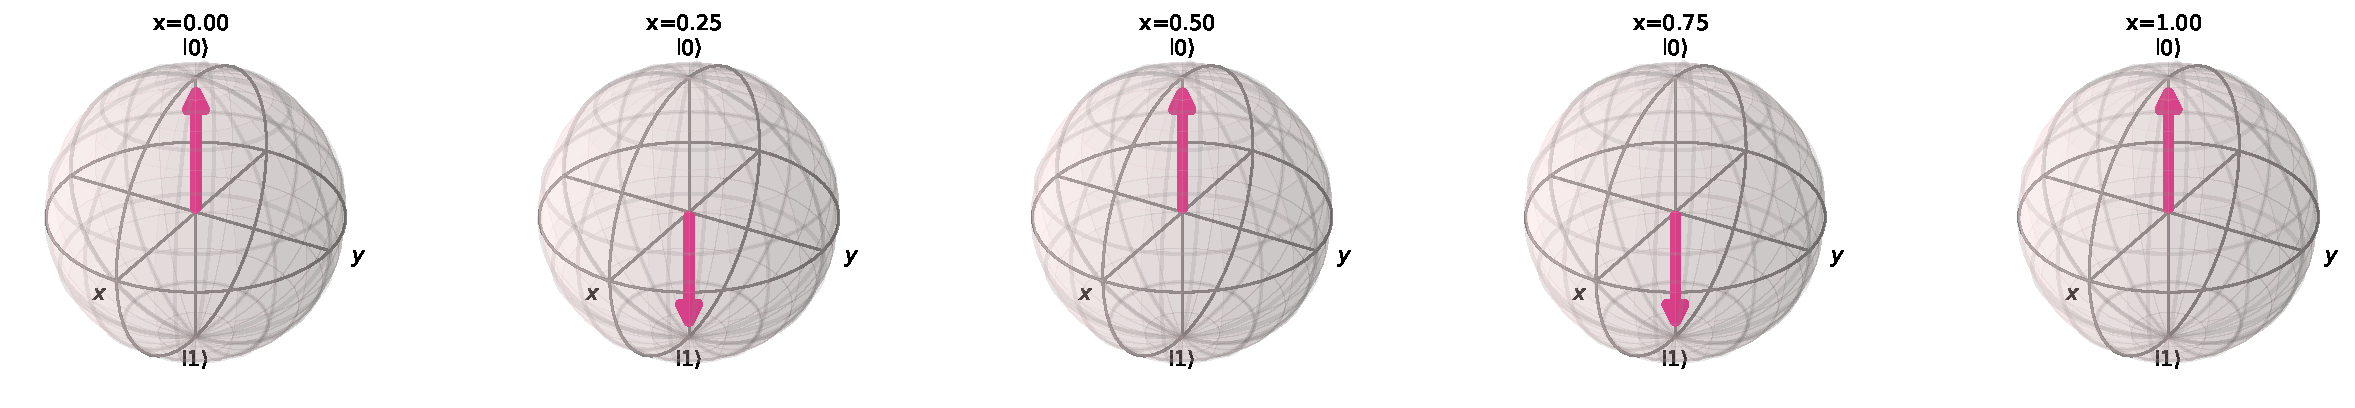
\includegraphics[keepaspectratio]{apostila_files/figure-pdf/cell-28-output-2.pdf}}

\begin{verbatim}

======================================================================
💡 Interpretação:
   Dados diferentes → Ângulos diferentes → Estados quânticos diferentes
   Assim, codificamos informação clássica em superposições quânticas!
======================================================================
\end{verbatim}

\begin{verbatim}
======================================================================
CODIFICAÇÃO DE DADOS CLÁSSICOS EM QUBITS
======================================================================

Dado clássico: x = 0.00
  Ângulo: θ = 2π × 0.00 = 0.0000 rad (0.0°)
  Estado: 1.0000+0.0000j|0⟩ + 0.0000+0.0000j|1⟩
  P(medir 1) = 0.0000

Dado clássico: x = 0.25
  Ângulo: θ = 2π × 0.25 = 1.5708 rad (90.0°)
  Estado: 0.7071+0.0000j|0⟩ + 0.7071+0.0000j|1⟩
  P(medir 1) = 0.5000

Dado clássico: x = 0.50
  Ângulo: θ = 2π × 0.50 = 3.1416 rad (180.0°)
  Estado: 0.0000+0.0000j|0⟩ + 1.0000+0.0000j|1⟩
  P(medir 1) = 1.0000

Dado clássico: x = 0.75
  Ângulo: θ = 2π × 0.75 = 4.7124 rad (270.0°)
  Estado: -0.7071+0.0000j|0⟩ + 0.7071+0.0000j|1⟩
  P(medir 1) = 0.5000

Dado clássico: x = 1.00
  Ângulo: θ = 2π × 1.00 = 6.2832 rad (360.0°)
  Estado: -1.0000+0.0000j|0⟩ + 0.0000+0.0000j|1⟩
  P(medir 1) = 0.0000
\end{verbatim}

\begin{verbatim}

======================================================================
💡 Interpretação:
   Dados diferentes → Ângulos diferentes → Estados quânticos diferentes
   Assim, codificamos informação clássica em superposições quânticas!
======================================================================
\end{verbatim}

\subsection{📊 Resumo: Portas de Rotação
Parametrizadas}\label{resumo-portas-de-rotauxe7uxe3o-parametrizadas}

\begin{longtable}[]{@{}lllll@{}}
\toprule\noalign{}
Porta & Eixo & Afeta & Uso Principal & Exemplo \\
\midrule\noalign{}
\endhead
\bottomrule\noalign{}
\endlastfoot
\textbf{RX(θ)} & X & Amplitude + Fase & Rotações YZ & Criar
\textbar i+⟩, \textbar i-⟩ \\
\textbf{RY(θ)} & Y & Amplitude (real) & \textbf{Ansatz, VQC} & Codificar
dados \\
\textbf{RZ(θ)} & Z & Fase apenas & \textbf{Feature Maps} &
ZZFeatureMap \\
\end{longtable}

\textbf{Relação com portas fixas:} - Z = RZ(π) --- rotação de 180° em Z
- S = RZ(π/2) --- rotação de 90° em Z - T = RZ(π/4) --- rotação de 45°
em Z - X = RX(π) --- rotação de 180° em X (porta NOT) - H ≠ rotação
simples (combinação de rotações)

\textbf{Por que são essenciais para Machine Learning Quântico?}

\begin{enumerate}
\def\labelenumi{\arabic{enumi}.}
\tightlist
\item
  \textbf{Parametrização}: Os ângulos θ são variáveis treináveis
\item
  \textbf{Expressividade}: Podem criar qualquer estado de 1 qubit
\item
  \textbf{Gradientes}: Permitem calcular derivadas para otimização
\item
  \textbf{Codificação}: Mapeiam features clássicas → amplitudes
  quânticas
\end{enumerate}

Nos próximos notebooks, você verá essas portas em ação no
\textbf{algoritmo de Grover} (interferência), \textbf{QFT} (fases), e
especialmente no \textbf{VQC} (otimização de ângulos)!

\section{Porta Controlled PhaseGate
(CP)}\label{porta-controlled-phasegate-cp}

A porta CP (Controlled Phase) é uma porta lógica quântica que atua em
dois qubits: um qubit de controle e um qubit alvo. A operação da porta
CP é a seguinte:

\begin{itemize}
\tightlist
\item
  Se o qubit de controle estiver em \textbar0⟩, o qubit alvo permanece
  inalterado.
\item
  Se o qubit de controle estiver em \textbar1⟩, a fase do qubit alvo é
  alterada por um ângulo específico φ (phi).
\end{itemize}

A porta CP é representada pela seguinte matriz:

\[
\text{CP}(φ) = 
\begin{bmatrix}
1 & 0 & 0 & 0 \\
0 & 1 & 0 & 0 \\
0 & 0 & 1 & 0 \\
0 & 0 & 0 & e^{iφ}
\end{bmatrix}
\]

Quando aplicamos a porta CP a um estado composto de dois qubits, o
resultado depende do estado do qubit de controle. Por exemplo, se
aplicarmos a porta CP ao estado \textbar11⟩ (onde o primeiro qubit é o
controle e o segundo é o alvo), o resultado será \(e^{iφ}|11⟩\), pois o
qubit de controle está em \textbar1⟩, então a fase do qubit alvo é
alterada por φ.

Por exemplo: \[
\text{CP}(φ)|11⟩ =
\begin{bmatrix}
1 & 0 & 0 & 0 \\
0 & 1 & 0 & 0 \\
0 & 0 & 1 & 0 \\
0 & 0 & 0 & e^{iφ}
\end{bmatrix} * 
\begin{bmatrix}
0 \\ 0 \\ 0 \\ 1
\end{bmatrix} =
\begin{bmatrix}
0 \\ 0 \\ 0 \\ e^{iφ}
\end{bmatrix} =
e^{iφ}|11⟩
\]

\subsubsection{Usando a Porta CP com Numpy puro (sem
Qiskit)}\label{usando-a-porta-cp-com-numpy-puro-sem-qiskit}

\begin{Shaded}
\begin{Highlighting}[]
\CommentTok{\# Implementação da porta CPHASE (Controlled{-}Phase)}

\KeywordTok{def}\NormalTok{ cphase\_gate(theta):}
    \ControlFlowTok{return}\NormalTok{ np.array([}
\NormalTok{        [}\DecValTok{1}\NormalTok{, }\DecValTok{0}\NormalTok{, }\DecValTok{0}\NormalTok{, }\DecValTok{0}\NormalTok{],}
\NormalTok{        [}\DecValTok{0}\NormalTok{, }\DecValTok{1}\NormalTok{, }\DecValTok{0}\NormalTok{, }\DecValTok{0}\NormalTok{],}
\NormalTok{        [}\DecValTok{0}\NormalTok{, }\DecValTok{0}\NormalTok{, }\DecValTok{1}\NormalTok{, }\DecValTok{0}\NormalTok{],}
\NormalTok{        [}\DecValTok{0}\NormalTok{, }\DecValTok{0}\NormalTok{, }\DecValTok{0}\NormalTok{, np.exp(}\OtherTok{1j} \OperatorTok{*}\NormalTok{ theta)]}
\NormalTok{    ])}
    
\CommentTok{\# Testando a porta CPHASE com θ = π/2}
\NormalTok{theta }\OperatorTok{=}\NormalTok{ np.pi }\OperatorTok{/} \DecValTok{2}
\NormalTok{CPHASE }\OperatorTok{=}\NormalTok{ cphase\_gate(theta)}

\CommentTok{\# |11\textgreater{}}
\NormalTok{q\_11 }\OperatorTok{=}\NormalTok{ np.array([}
\NormalTok{    [}\DecValTok{0}\NormalTok{],}
\NormalTok{    [}\DecValTok{0}\NormalTok{],}
\NormalTok{    [}\DecValTok{0}\NormalTok{],}
\NormalTok{    [}\DecValTok{1}\NormalTok{]}
\NormalTok{])}

\CommentTok{\# Aplicando a porta CPHASE em |11\textgreater{}}
\NormalTok{novo\_estado\_cphase }\OperatorTok{=}\NormalTok{ np.dot(CPHASE, q\_11)}

\BuiltInTok{print}\NormalTok{(}\StringTok{"}\CharTok{\textbackslash{}n}\StringTok{{-}{-}{-} Após aplicar a Porta CPHASE em |11\textgreater{} com θ=π/2 {-}{-}{-}"}\NormalTok{)}
\BuiltInTok{print}\NormalTok{(}\SpecialStringTok{f"Esperamos e\^{}(iπ/2)|11\textgreater{} = i|11\textgreater{}, obtivemos:}\CharTok{\textbackslash{}n}\SpecialCharTok{\{}\NormalTok{novo\_estado\_cphase}\SpecialCharTok{\}}\SpecialStringTok{"}\NormalTok{)}
\BuiltInTok{print}\NormalTok{(}\StringTok{"}\CharTok{\textbackslash{}n}\StringTok{✅ A porta CPHASE funcionou como esperado! (aplicou a fase correta em |11\textgreater{})"}\NormalTok{)}
\end{Highlighting}
\end{Shaded}

\begin{verbatim}

--- Após aplicar a Porta CPHASE em |11> com θ=π/2 ---
Esperamos e^(iπ/2)|11> = i|11>, obtivemos:
[[0.000000e+00+0.j]
 [0.000000e+00+0.j]
 [0.000000e+00+0.j]
 [6.123234e-17+1.j]]

✅ A porta CPHASE funcionou como esperado! (aplicou a fase correta em |11>)
\end{verbatim}

\begin{verbatim}

--- Após aplicar a Porta CPHASE em |11> com θ=π/2 ---
Esperamos e^(iπ/2)|11> = i|11>, obtivemos:
[[0.000000e+00+0.j]
 [0.000000e+00+0.j]
 [0.000000e+00+0.j]
 [6.123234e-17+1.j]]

✅ A porta CPHASE funcionou como esperado! (aplicou a fase correta em |11>)
\end{verbatim}

Vamos ver outro exemplo utilizando a esfera de Bloch para visualizar o
efeito da porta CP em um sistema de dois qubits.

\begin{Shaded}
\begin{Highlighting}[]
\CommentTok{\# Visualização do efeito da Porta CPHASE nas Esferas de Bloch}
\ImportTok{import}\NormalTok{ numpy }\ImportTok{as}\NormalTok{ np}
\ImportTok{from}\NormalTok{ qiskit.quantum\_info }\ImportTok{import}\NormalTok{ Statevector}
\ImportTok{from}\NormalTok{ qiskit.visualization }\ImportTok{import}\NormalTok{ plot\_bloch\_multivector}
\ImportTok{import}\NormalTok{ matplotlib.pyplot }\ImportTok{as}\NormalTok{ plt}
\ImportTok{from}\NormalTok{ IPython.display }\ImportTok{import}\NormalTok{ display, Markdown}
\end{Highlighting}
\end{Shaded}

Vamos criar o estado passo a passo para entender como ele aparece nas
esferas de Bloch:

\textbf{O que queremos:} - Qubit 1 (controle): estado \textbar+⟩ →
aparece no \textbf{equador} (direção +X) - Qubit 0 (alvo): estado
\textbar1⟩ → aparece no \textbf{polo sul}

\textbf{Como fazer com \texttt{np.kron}:}

A função \texttt{np.kron(A,\ B)} em NumPy significa ``produto tensorial
A ⊗ B'', onde: - \textbf{A} = primeiro argumento → vira o \textbf{qubit
mais significativo} (qubit 1 no Qiskit) - \textbf{B} = segundo argumento
→ vira o \textbf{qubit menos significativo} (qubit 0 no Qiskit)

Portanto:

\begin{Shaded}
\begin{Highlighting}[]
\NormalTok{np.kron(}\OperatorTok{|+}\NormalTok{⟩, }\OperatorTok{|}\DecValTok{1}\NormalTok{⟩)  →  qubit1 }\OperatorTok{=} \OperatorTok{|+}\NormalTok{⟩  e  qubit0 }\OperatorTok{=} \OperatorTok{|}\DecValTok{1}\NormalTok{⟩}
\end{Highlighting}
\end{Shaded}

\textbf{Na visualização Bloch:} - \textbf{Esfera da ESQUERDA} = qubit 0
(menos significativo) = \textbar1⟩ → \textbf{polo sul} ✓ -
\textbf{Esfera da DIREITA} = qubit 1 (mais significativo) = \textbar+⟩ →
\textbf{equador +X} ✓

\begin{Shaded}
\begin{Highlighting}[]
\CommentTok{\# Parâmetro da porta (já definido no notebook): θ = π/2}
\NormalTok{theta }\OperatorTok{=}\NormalTok{ np.pi }\OperatorTok{/} \DecValTok{2}
\NormalTok{CP }\OperatorTok{=}\NormalTok{ cphase\_gate(theta)}

\BuiltInTok{print}\NormalTok{(}\StringTok{"="} \OperatorTok{*} \DecValTok{70}\NormalTok{)}
\BuiltInTok{print}\NormalTok{(}\StringTok{"CRIANDO O ESTADO QUÂNTICO DE 2 QUBITS"}\NormalTok{)}
\BuiltInTok{print}\NormalTok{(}\StringTok{"="} \OperatorTok{*} \DecValTok{70}\NormalTok{)}

\CommentTok{\# Definir os estados individuais}
\NormalTok{estado\_qubit1 }\OperatorTok{=} \DecValTok{1}\OperatorTok{/}\NormalTok{np.sqrt(}\DecValTok{2}\NormalTok{) }\OperatorTok{*}\NormalTok{ np.array([}\DecValTok{1}\NormalTok{, }\DecValTok{1}\NormalTok{])   }\CommentTok{\# |+⟩ para qubit 1}
\NormalTok{estado\_qubit0 }\OperatorTok{=}\NormalTok{ np.array([}\DecValTok{0}\NormalTok{, }\DecValTok{1}\NormalTok{])                  }\CommentTok{\# |1⟩ para qubit 0}

\BuiltInTok{print}\NormalTok{(}\StringTok{"}\CharTok{\textbackslash{}n}\StringTok{1️⃣ Estado do qubit 1 (controle):"}\NormalTok{)}
\BuiltInTok{print}\NormalTok{(}\SpecialStringTok{f"   |+⟩ = 1/√2 (|0⟩ + |1⟩)"}\NormalTok{)}
\BuiltInTok{print}\NormalTok{(}\SpecialStringTok{f"   Vetor: }\SpecialCharTok{\{}\NormalTok{estado\_qubit1}\SpecialCharTok{\}}\SpecialStringTok{"}\NormalTok{)}
\BuiltInTok{print}\NormalTok{(}\StringTok{"   → Na esfera de Bloch: equador, direção +X"}\NormalTok{)}

\BuiltInTok{print}\NormalTok{(}\StringTok{"}\CharTok{\textbackslash{}n}\StringTok{2️⃣ Estado do qubit 0 (alvo):"}\NormalTok{)}
\BuiltInTok{print}\NormalTok{(}\SpecialStringTok{f"   |1⟩"}\NormalTok{)}
\BuiltInTok{print}\NormalTok{(}\SpecialStringTok{f"   Vetor: }\SpecialCharTok{\{}\NormalTok{estado\_qubit0}\SpecialCharTok{\}}\SpecialStringTok{"}\NormalTok{)}
\BuiltInTok{print}\NormalTok{(}\StringTok{"   → Na esfera de Bloch: polo sul"}\NormalTok{)}

\CommentTok{\# Criar o estado composto usando produto tensorial (Kronecker)}
\NormalTok{state\_before }\OperatorTok{=}\NormalTok{ np.kron(estado\_qubit1, estado\_qubit0)}
\NormalTok{sv\_before }\OperatorTok{=}\NormalTok{ Statevector(state\_before)}

\BuiltInTok{print}\NormalTok{(}\StringTok{"}\CharTok{\textbackslash{}n}\StringTok{3️⃣ Estado composto (produto tensorial):"}\NormalTok{)}
\BuiltInTok{print}\NormalTok{(}\SpecialStringTok{f"   np.kron(|+⟩, |1⟩) = |+⟩ ⊗ |1⟩"}\NormalTok{)}
\NormalTok{display(Markdown(}\VerbatimStringTok{r"}\DecValTok{$$}\VerbatimStringTok{= }\CharTok{\textbackslash{}f}\VerbatimStringTok{rac}\OperatorTok{\{1\}}\VerbatimStringTok{\{}\DecValTok{\textbackslash{}s}\VerbatimStringTok{qrt}\OperatorTok{\{2\}}\VerbatimStringTok{\}}\KeywordTok{(}\ControlFlowTok{|}\VerbatimStringTok{0}\CharTok{\textbackslash{}r}\VerbatimStringTok{angle }\OperatorTok{+}\VerbatimStringTok{ }\ControlFlowTok{|}\VerbatimStringTok{1}\CharTok{\textbackslash{}r}\VerbatimStringTok{angle}\KeywordTok{)}\VerbatimStringTok{ }\ErrorTok{\textbackslash{}}\VerbatimStringTok{otimes }\ControlFlowTok{|}\VerbatimStringTok{1}\CharTok{\textbackslash{}r}\VerbatimStringTok{angle = }\CharTok{\textbackslash{}f}\VerbatimStringTok{rac}\OperatorTok{\{1\}}\VerbatimStringTok{\{}\DecValTok{\textbackslash{}s}\VerbatimStringTok{qrt}\OperatorTok{\{2\}}\VerbatimStringTok{\}}\KeywordTok{(}\ControlFlowTok{|}\VerbatimStringTok{01}\CharTok{\textbackslash{}r}\VerbatimStringTok{angle }\OperatorTok{+}\VerbatimStringTok{ }\ControlFlowTok{|}\VerbatimStringTok{11}\CharTok{\textbackslash{}r}\VerbatimStringTok{angle}\KeywordTok{)}\DecValTok{$$}\VerbatimStringTok{"}\NormalTok{))}

\BuiltInTok{print}\NormalTok{(}\StringTok{"}\CharTok{\textbackslash{}n}\StringTok{4️⃣ Vetor estado final (4 componentes):"}\NormalTok{)}
\NormalTok{display(Markdown(}\VerbatimStringTok{r"""}\DecValTok{$$\textbackslash{}b}\VerbatimStringTok{egin\{bmatrix\}0 }\CharTok{\textbackslash{}\textbackslash{}}\VerbatimStringTok{ }\CharTok{\textbackslash{}f}\VerbatimStringTok{rac}\OperatorTok{\{1\}}\VerbatimStringTok{\{}\DecValTok{\textbackslash{}s}\VerbatimStringTok{qrt}\OperatorTok{\{2\}}\VerbatimStringTok{\} }\CharTok{\textbackslash{}\textbackslash{}}\VerbatimStringTok{ 0 }\CharTok{\textbackslash{}\textbackslash{}}\VerbatimStringTok{ }\CharTok{\textbackslash{}f}\VerbatimStringTok{rac}\OperatorTok{\{1\}}\VerbatimStringTok{\{}\DecValTok{\textbackslash{}s}\VerbatimStringTok{qrt}\OperatorTok{\{2\}}\VerbatimStringTok{\} }\ErrorTok{\textbackslash{}}\VerbatimStringTok{end\{bmatrix\} }\DecValTok{\textbackslash{}b}\VerbatimStringTok{egin\{array\}\{l\} }\ErrorTok{\textbackslash{}}\VerbatimStringTok{leftarrow }\ControlFlowTok{|}\VerbatimStringTok{00}\CharTok{\textbackslash{}r}\VerbatimStringTok{angle }\CharTok{\textbackslash{}t}\VerbatimStringTok{ext\{ }\KeywordTok{(}\VerbatimStringTok{qubit1=0, qubit0=0}\KeywordTok{)}\VerbatimStringTok{\} }\CharTok{\textbackslash{}\textbackslash{}}\VerbatimStringTok{ }\ErrorTok{\textbackslash{}}\VerbatimStringTok{leftarrow }\ControlFlowTok{|}\VerbatimStringTok{01}\CharTok{\textbackslash{}r}\VerbatimStringTok{angle }\CharTok{\textbackslash{}t}\VerbatimStringTok{ext\{ }\KeywordTok{(}\VerbatimStringTok{qubit1=0, qubit0=1}\KeywordTok{)}\VerbatimStringTok{\} ✓ }\CharTok{\textbackslash{}\textbackslash{}}\VerbatimStringTok{ }\ErrorTok{\textbackslash{}}\VerbatimStringTok{leftarrow }\ControlFlowTok{|}\VerbatimStringTok{10}\CharTok{\textbackslash{}r}\VerbatimStringTok{angle }\CharTok{\textbackslash{}t}\VerbatimStringTok{ext\{ }\KeywordTok{(}\VerbatimStringTok{qubit1=1, qubit0=0}\KeywordTok{)}\VerbatimStringTok{\} }\CharTok{\textbackslash{}\textbackslash{}}\VerbatimStringTok{ }\ErrorTok{\textbackslash{}}\VerbatimStringTok{leftarrow }\ControlFlowTok{|}\VerbatimStringTok{11}\CharTok{\textbackslash{}r}\VerbatimStringTok{angle }\CharTok{\textbackslash{}t}\VerbatimStringTok{ext\{ }\KeywordTok{(}\VerbatimStringTok{qubit1=1, qubit0=1}\KeywordTok{)}\VerbatimStringTok{\} ✓ }\ErrorTok{\textbackslash{}}\VerbatimStringTok{end\{array\}}\DecValTok{$$}\VerbatimStringTok{"""}\NormalTok{))}

\BuiltInTok{print}\NormalTok{(}\StringTok{"}\CharTok{\textbackslash{}n}\StringTok{💡 Interpretação:"}\NormalTok{)}
\BuiltInTok{print}\NormalTok{(}\StringTok{"   • Componentes |01⟩ e |11⟩ têm amplitude 1/√2 (50}\SpecialCharTok{\% d}\StringTok{e probabilidade cada)"}\NormalTok{)}
\BuiltInTok{print}\NormalTok{(}\StringTok{"   • Qubit 0 está SEMPRE em |1⟩ (polo sul)"}\NormalTok{)}
\BuiltInTok{print}\NormalTok{(}\StringTok{"   • Qubit 1 está em superposição |+⟩ (equador +X)"}\NormalTok{)}
\BuiltInTok{print}\NormalTok{(}\StringTok{"="} \OperatorTok{*} \DecValTok{70}\NormalTok{)}
\end{Highlighting}
\end{Shaded}

\begin{verbatim}
======================================================================
CRIANDO O ESTADO QUÂNTICO DE 2 QUBITS
======================================================================

1️⃣ Estado do qubit 1 (controle):
   |+⟩ = 1/√2 (|0⟩ + |1⟩)
   Vetor: [0.70710678 0.70710678]
   → Na esfera de Bloch: equador, direção +X

2️⃣ Estado do qubit 0 (alvo):
   |1⟩
   Vetor: [0 1]
   → Na esfera de Bloch: polo sul

3️⃣ Estado composto (produto tensorial):
   np.kron(|+⟩, |1⟩) = |+⟩ ⊗ |1⟩
\end{verbatim}

\[= \frac{1}{\sqrt{2}}(|0\rangle + |1\rangle) \otimes |1\rangle = \frac{1}{\sqrt{2}}(|01\rangle + |11\rangle)\]

\begin{verbatim}

4️⃣ Vetor estado final (4 componentes):
\end{verbatim}

\[\begin{bmatrix}0 \\ \frac{1}{\sqrt{2}} \\ 0 \\ \frac{1}{\sqrt{2}} \end{bmatrix} \begin{array}{l} \leftarrow |00\rangle \text{ (qubit1=0, qubit0=0)} \\ \leftarrow |01\rangle \text{ (qubit1=0, qubit0=1)} ✓ \\ \leftarrow |10\rangle \text{ (qubit1=1, qubit0=0)} \\ \leftarrow |11\rangle \text{ (qubit1=1, qubit0=1)} ✓ \end{array}\]

\begin{verbatim}

💡 Interpretação:
   • Componentes |01⟩ e |11⟩ têm amplitude 1/√2 (50% de probabilidade cada)
   • Qubit 0 está SEMPRE em |1⟩ (polo sul)
   • Qubit 1 está em superposição |+⟩ (equador +X)
======================================================================
\end{verbatim}

\begin{verbatim}
======================================================================
CRIANDO O ESTADO QUÂNTICO DE 2 QUBITS
======================================================================

1️⃣ Estado do qubit 1 (controle):
   |+⟩ = 1/√2 (|0⟩ + |1⟩)
   Vetor: [0.70710678 0.70710678]
   → Na esfera de Bloch: equador, direção +X

2️⃣ Estado do qubit 0 (alvo):
   |1⟩
   Vetor: [0 1]
   → Na esfera de Bloch: polo sul

3️⃣ Estado composto (produto tensorial):
   np.kron(|+⟩, |1⟩) = |+⟩ ⊗ |1⟩
\end{verbatim}

\begin{verbatim}

4️⃣ Vetor estado final (4 componentes):
\end{verbatim}

\begin{verbatim}

💡 Interpretação:
   • Componentes |01⟩ e |11⟩ têm amplitude 1/√2 (50% de probabilidade cada)
   • Qubit 0 está SEMPRE em |1⟩ (polo sul)
   • Qubit 1 está em superposição |+⟩ (equador +X)
======================================================================
\end{verbatim}

\begin{Shaded}
\begin{Highlighting}[]
\BuiltInTok{print}\NormalTok{(}\StringTok{"Antes da CP (controle |+\textgreater{}, alvo |1\textgreater{}):"}\NormalTok{)}
\NormalTok{display(plot\_bloch\_multivector(sv\_before))}
\end{Highlighting}
\end{Shaded}

\begin{verbatim}
Antes da CP (controle |+>, alvo |1>):
\end{verbatim}

\pandocbounded{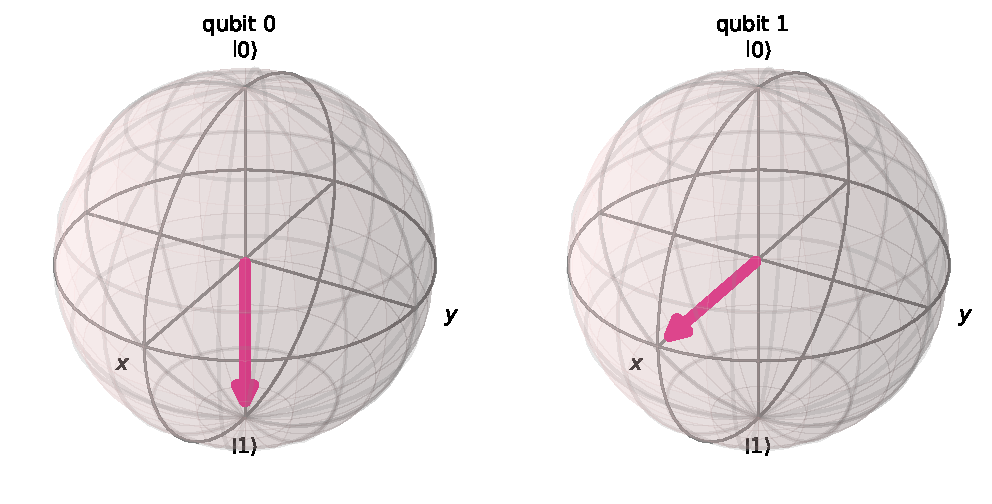
\includegraphics[keepaspectratio]{apostila_files/figure-pdf/cell-32-output-2.pdf}}

\begin{verbatim}
Antes da CP (controle |+>, alvo |1>):
\end{verbatim}

\begin{Shaded}
\begin{Highlighting}[]
\CommentTok{\# Aplicar CPHASE}
\NormalTok{state\_after }\OperatorTok{=}\NormalTok{ CP.dot(state\_before.reshape(}\DecValTok{4}\NormalTok{, }\DecValTok{1}\NormalTok{)).flatten()}
\NormalTok{sv\_after }\OperatorTok{=}\NormalTok{ Statevector(state\_after)}

\BuiltInTok{print}\NormalTok{(}\StringTok{"Depois da CP (θ = π/2):"}\NormalTok{)}
\NormalTok{display(plot\_bloch\_multivector(sv\_after))}
\end{Highlighting}
\end{Shaded}

\begin{verbatim}
Depois da CP (θ = π/2):
\end{verbatim}

\pandocbounded{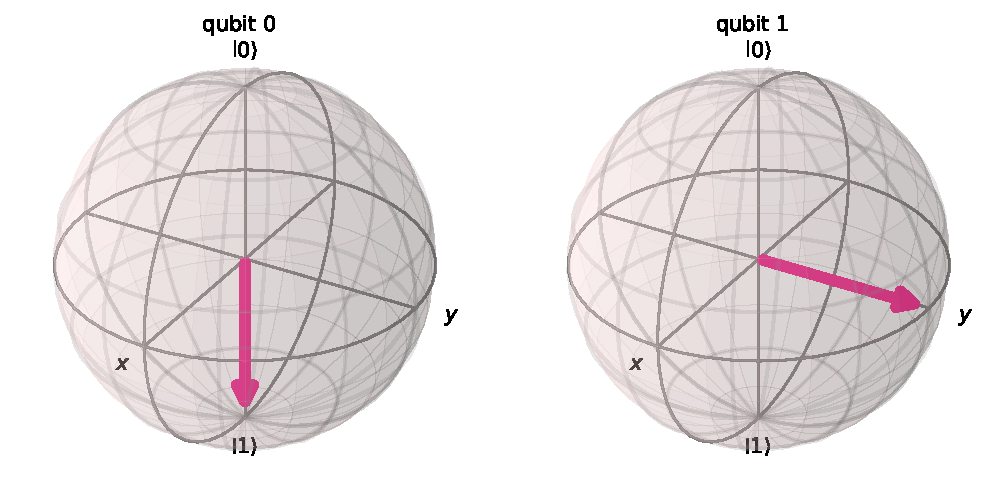
\includegraphics[keepaspectratio]{apostila_files/figure-pdf/cell-33-output-2.pdf}}

\begin{verbatim}
Depois da CP (θ = π/2):
\end{verbatim}

\begin{Shaded}
\begin{Highlighting}[]
\CommentTok{\# Análise numérica do estado reduzido do qubit alvo}
\NormalTok{psi\_before }\OperatorTok{=}\NormalTok{ state\_before.reshape((}\DecValTok{2}\NormalTok{, }\DecValTok{2}\NormalTok{))    }\CommentTok{\# formato (controle, alvo)}
\NormalTok{rho\_target\_before }\OperatorTok{=}\NormalTok{ np.conj(psi\_before).T }\OperatorTok{@}\NormalTok{ psi\_before}
\NormalTok{psi\_after }\OperatorTok{=}\NormalTok{ state\_after.reshape((}\DecValTok{2}\NormalTok{, }\DecValTok{2}\NormalTok{))}
\NormalTok{rho\_target\_after }\OperatorTok{=}\NormalTok{ np.conj(psi\_after).T }\OperatorTok{@}\NormalTok{ psi\_after}

\KeywordTok{def}\NormalTok{ bloch\_coords\_from\_rho(rho):}
\NormalTok{    r01 }\OperatorTok{=}\NormalTok{ rho[}\DecValTok{0}\NormalTok{,}\DecValTok{1}\NormalTok{]}
\NormalTok{    x }\OperatorTok{=} \DecValTok{2} \OperatorTok{*}\NormalTok{ r01.real}
\NormalTok{    y }\OperatorTok{=} \OperatorTok{{-}}\DecValTok{2} \OperatorTok{*}\NormalTok{ r01.imag}
\NormalTok{    z }\OperatorTok{=}\NormalTok{ rho[}\DecValTok{0}\NormalTok{,}\DecValTok{0}\NormalTok{].real }\OperatorTok{{-}}\NormalTok{ rho[}\DecValTok{1}\NormalTok{,}\DecValTok{1}\NormalTok{].real}
    \ControlFlowTok{return}\NormalTok{ x, y, z}

\NormalTok{x1, y1, z1 }\OperatorTok{=}\NormalTok{ bloch\_coords\_from\_rho(rho\_target\_before)}
\NormalTok{x2, y2, z2 }\OperatorTok{=}\NormalTok{ bloch\_coords\_from\_rho(rho\_target\_after)}

\BuiltInTok{print}\NormalTok{(}\SpecialStringTok{f"}\CharTok{\textbackslash{}n}\SpecialStringTok{Qubit alvo {-} Bloch coords antes: x=}\SpecialCharTok{\{}\NormalTok{x1}\SpecialCharTok{:.3f\}}\SpecialStringTok{, y=}\SpecialCharTok{\{}\NormalTok{y1}\SpecialCharTok{:.3f\}}\SpecialStringTok{, z=}\SpecialCharTok{\{}\NormalTok{z1}\SpecialCharTok{:.3f\}}\SpecialStringTok{"}\NormalTok{)}
\BuiltInTok{print}\NormalTok{(}\SpecialStringTok{f"Qubit alvo {-} Bloch coords depois: x=}\SpecialCharTok{\{}\NormalTok{x2}\SpecialCharTok{:.3f\}}\SpecialStringTok{, y=}\SpecialCharTok{\{}\NormalTok{y2}\SpecialCharTok{:.3f\}}\SpecialStringTok{, z=}\SpecialCharTok{\{}\NormalTok{z2}\SpecialCharTok{:.3f\}}\SpecialStringTok{"}\NormalTok{)}

\CommentTok{\# Mostrar a mudança de fase na componente |11\textgreater{}}
\NormalTok{amp\_11\_before }\OperatorTok{=}\NormalTok{ state\_before[}\DecValTok{3}\NormalTok{]}
\NormalTok{amp\_11\_after }\OperatorTok{=}\NormalTok{ state\_after[}\DecValTok{3}\NormalTok{]}
\BuiltInTok{print}\NormalTok{(}\SpecialStringTok{f"}\CharTok{\textbackslash{}n}\SpecialStringTok{Amplitude |11\textgreater{} antes: }\SpecialCharTok{\{}\NormalTok{amp\_11\_before}\SpecialCharTok{\}}\SpecialStringTok{, fase=}\SpecialCharTok{\{}\NormalTok{np}\SpecialCharTok{.}\NormalTok{angle(amp\_11\_before, deg}\OperatorTok{=}\VariableTok{True}\NormalTok{)}\SpecialCharTok{:.2f\}}\SpecialStringTok{°"}\NormalTok{)}
\BuiltInTok{print}\NormalTok{(}\SpecialStringTok{f"Amplitude |11\textgreater{} depois: }\SpecialCharTok{\{}\NormalTok{amp\_11\_after}\SpecialCharTok{\}}\SpecialStringTok{, fase=}\SpecialCharTok{\{}\NormalTok{np}\SpecialCharTok{.}\NormalTok{angle(amp\_11\_after, deg}\OperatorTok{=}\VariableTok{True}\NormalTok{)}\SpecialCharTok{:.2f\}}\SpecialStringTok{°"}\NormalTok{)}
\end{Highlighting}
\end{Shaded}

\begin{verbatim}

Qubit alvo - Bloch coords antes: x=0.000, y=-0.000, z=-1.000
Qubit alvo - Bloch coords depois: x=0.000, y=-0.000, z=-1.000

Amplitude |11> antes: 0.7071067811865475, fase=0.00°
Amplitude |11> depois: (4.329780281177466e-17+0.7071067811865475j), fase=90.00°
\end{verbatim}

\begin{verbatim}

Qubit alvo - Bloch coords antes: x=0.000, y=-0.000, z=-1.000
Qubit alvo - Bloch coords depois: x=0.000, y=-0.000, z=-1.000

Amplitude |11> antes: 0.7071067811865475, fase=0.00°
Amplitude |11> depois: (4.329780281177466e-17+0.7071067811865475j), fase=90.00°
\end{verbatim}

\subsubsection{Usando a Porta CP com
Qiskit}\label{usando-a-porta-cp-com-qiskit}

Até agora trabalhamos com NumPy e vetores de estado diretamente. Agora
vamos ver como usar a porta \textbf{CP (Controlled-Phase)} no Qiskit,
que é a biblioteca padrão para criar circuitos quânticos.

No Qiskit, a porta CP está disponível como
\texttt{qc.cp(theta,\ control\_qubit,\ target\_qubit)}.

\begin{Shaded}
\begin{Highlighting}[]
\ImportTok{from}\NormalTok{ qiskit }\ImportTok{import}\NormalTok{ QuantumCircuit}
\ImportTok{from}\NormalTok{ qiskit.quantum\_info }\ImportTok{import}\NormalTok{ Statevector}
\ImportTok{from}\NormalTok{ qiskit.visualization }\ImportTok{import}\NormalTok{ plot\_bloch\_multivector}
\ImportTok{import}\NormalTok{ matplotlib.pyplot }\ImportTok{as}\NormalTok{ plt}
\ImportTok{import}\NormalTok{ numpy }\ImportTok{as}\NormalTok{ np}

\CommentTok{\# Criar um circuito com 2 qubits}
\NormalTok{qc }\OperatorTok{=}\NormalTok{ QuantumCircuit(}\DecValTok{2}\NormalTok{)}

\CommentTok{\# Preparar o estado inicial: qubit 1 em |+⟩ e qubit 0 em |1⟩}
\NormalTok{qc.h(}\DecValTok{1}\NormalTok{)      }\CommentTok{\# Hadamard no qubit 1 para criar |+⟩}
\NormalTok{qc.x(}\DecValTok{0}\NormalTok{)      }\CommentTok{\# Porta X no qubit 0 para criar |1⟩}

\BuiltInTok{print}\NormalTok{(}\StringTok{"Circuito ANTES da porta CP:"}\NormalTok{)}
\NormalTok{display(qc.draw(}\StringTok{\textquotesingle{}mpl\textquotesingle{}}\NormalTok{))}

\CommentTok{\# Salvar estado antes da CP}
\NormalTok{estado\_antes\_qiskit }\OperatorTok{=}\NormalTok{ Statevector(qc)}
\end{Highlighting}
\end{Shaded}

\begin{verbatim}
Circuito ANTES da porta CP:
\end{verbatim}

\pandocbounded{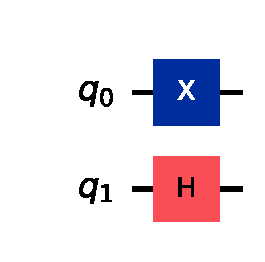
\includegraphics[keepaspectratio]{apostila_files/figure-pdf/cell-35-output-2.pdf}}

\begin{verbatim}
Circuito ANTES da porta CP:
\end{verbatim}

\begin{Shaded}
\begin{Highlighting}[]
\CommentTok{\# Aplicar a porta CP (Controlled{-}Phase) com θ = π/2}
\NormalTok{theta }\OperatorTok{=}\NormalTok{ np.pi }\OperatorTok{/} \DecValTok{2}
\NormalTok{qc.cp(theta, }\DecValTok{1}\NormalTok{, }\DecValTok{0}\NormalTok{)  }\CommentTok{\# Porta CP: controle=qubit1, alvo=qubit0}

\BuiltInTok{print}\NormalTok{(}\StringTok{"Circuito DEPOIS da porta CP:"}\NormalTok{)}
\NormalTok{display(qc.draw(}\StringTok{\textquotesingle{}mpl\textquotesingle{}}\NormalTok{))}

\CommentTok{\# Obter o estado final}
\NormalTok{estado\_depois\_qiskit }\OperatorTok{=}\NormalTok{ Statevector(qc)}
\end{Highlighting}
\end{Shaded}

\begin{verbatim}
Circuito DEPOIS da porta CP:
\end{verbatim}

\pandocbounded{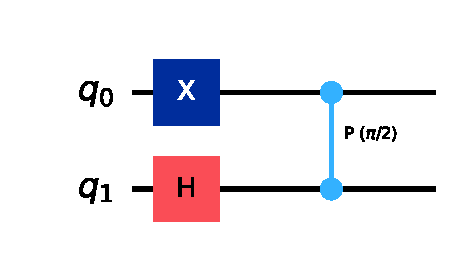
\includegraphics[keepaspectratio]{apostila_files/figure-pdf/cell-36-output-2.pdf}}

\begin{verbatim}
Circuito DEPOIS da porta CP:
\end{verbatim}

\begin{Shaded}
\begin{Highlighting}[]
\CommentTok{\# Comparar com o resultado NumPy anterior}
\BuiltInTok{print}\NormalTok{(}\StringTok{"="}\OperatorTok{*}\DecValTok{70}\NormalTok{)}
\BuiltInTok{print}\NormalTok{(}\StringTok{"COMPARAÇÃO: NumPy vs Qiskit"}\NormalTok{)}
\BuiltInTok{print}\NormalTok{(}\StringTok{"="}\OperatorTok{*}\DecValTok{70}\NormalTok{)}

\CommentTok{\# Formatação mais clara da comparação NumPy vs Qiskit}
\KeywordTok{def}\NormalTok{ state\_markdown(vec, label):}
\NormalTok{    lines }\OperatorTok{=}\NormalTok{ [}\SpecialStringTok{f"**}\SpecialCharTok{\{}\NormalTok{label}\SpecialCharTok{\}}\SpecialStringTok{**  "}\NormalTok{]}
    \ControlFlowTok{for}\NormalTok{ idx, amp }\KeywordTok{in} \BuiltInTok{enumerate}\NormalTok{(np.asarray(vec).flatten()):}
\NormalTok{        mag }\OperatorTok{=} \BuiltInTok{abs}\NormalTok{(amp)}
\NormalTok{        ph }\OperatorTok{=}\NormalTok{ np.angle(amp, deg}\OperatorTok{=}\VariableTok{True}\NormalTok{)}
\NormalTok{        lines.append(}\SpecialStringTok{f"{-} |}\SpecialCharTok{\{}\NormalTok{idx}\SpecialCharTok{:02b\}}\SpecialStringTok{\textgreater{} : amp = }\SpecialCharTok{\{}\NormalTok{mag}\SpecialCharTok{:.6f\}}\SpecialStringTok{ , fase = }\SpecialCharTok{\{}\NormalTok{ph}\SpecialCharTok{:7.2f\}}\SpecialStringTok{° , valor = }\SpecialCharTok{\{}\NormalTok{amp}\SpecialCharTok{\}}\SpecialStringTok{"}\NormalTok{)}
    \ControlFlowTok{return} \StringTok{"  }\CharTok{\textbackslash{}n}\StringTok{"}\NormalTok{.join(lines)}

\NormalTok{display(Markdown(}\StringTok{"\#\#\# 🔍 Comparação: NumPy vs Qiskit"}\NormalTok{))}
\NormalTok{display(Markdown(state\_markdown(state\_before, }\StringTok{"Antes (NumPy)"}\NormalTok{)))}
\NormalTok{display(Markdown(state\_markdown(estado\_antes\_qiskit.data, }\StringTok{"Antes (Qiskit)"}\NormalTok{)))}
\NormalTok{maxdiff\_before }\OperatorTok{=}\NormalTok{ np.}\BuiltInTok{max}\NormalTok{(np.}\BuiltInTok{abs}\NormalTok{(state\_before }\OperatorTok{{-}}\NormalTok{ estado\_antes\_qiskit.data))}
\NormalTok{display(Markdown(}\SpecialStringTok{f"**Diferença máxima (antes):** }\SpecialCharTok{\{}\NormalTok{maxdiff\_before}\SpecialCharTok{:.10e\}}\SpecialStringTok{"}\NormalTok{))}

\NormalTok{display(Markdown(}\StringTok{"\textless{}hr /\textgreater{}"}\NormalTok{))}

\NormalTok{display(Markdown(state\_markdown(state\_after, }\StringTok{"Depois (NumPy)"}\NormalTok{)))}
\NormalTok{display(Markdown(state\_markdown(estado\_depois\_qiskit.data, }\StringTok{"Depois (Qiskit)"}\NormalTok{)))}
\NormalTok{maxdiff\_after }\OperatorTok{=}\NormalTok{ np.}\BuiltInTok{max}\NormalTok{(np.}\BuiltInTok{abs}\NormalTok{(state\_after }\OperatorTok{{-}}\NormalTok{ estado\_depois\_qiskit.data))}
\NormalTok{display(Markdown(}\SpecialStringTok{f"**Diferença máxima (depois):** }\SpecialCharTok{\{}\NormalTok{maxdiff\_after}\SpecialCharTok{:.10e\}}\SpecialStringTok{"}\NormalTok{))}

\ControlFlowTok{if}\NormalTok{ np.allclose(state\_before, estado\_antes\_qiskit.data, atol}\OperatorTok{=}\FloatTok{1e{-}10}\NormalTok{) }\KeywordTok{and}\NormalTok{ np.allclose(state\_after, estado\_depois\_qiskit.data, atol}\OperatorTok{=}\FloatTok{1e{-}10}\NormalTok{):}
\NormalTok{    display(Markdown(}\StringTok{"✅ **Resultados idênticos dentro da tolerância numérica (atol=1e{-}10).**"}\NormalTok{))}
\ControlFlowTok{else}\NormalTok{:}
\NormalTok{    display(Markdown(}\StringTok{"⚠️ **Diferenças detectadas — verifique tolerâncias e fases.**"}\NormalTok{))}

\CommentTok{\# Resumo focalizado na componente |11\textgreater{}}
\NormalTok{idx }\OperatorTok{=} \DecValTok{3}
\NormalTok{phase\_before }\OperatorTok{=}\NormalTok{ np.angle(state\_before[idx], deg}\OperatorTok{=}\VariableTok{True}\NormalTok{)}
\NormalTok{phase\_after }\OperatorTok{=}\NormalTok{ np.angle(state\_after[idx], deg}\OperatorTok{=}\VariableTok{True}\NormalTok{)}
\NormalTok{display(Markdown(}
    \SpecialStringTok{f"**Componente |11\textgreater{}:**  }\CharTok{\textbackslash{}n}\SpecialStringTok{"}
    \SpecialStringTok{f"{-} NumPy: amp = }\SpecialCharTok{\{}\BuiltInTok{abs}\NormalTok{(state\_before[idx])}\SpecialCharTok{:.6f\}}\SpecialStringTok{, fase = }\SpecialCharTok{\{}\NormalTok{phase\_before}\SpecialCharTok{:7.2f\}}\SpecialStringTok{°  }\CharTok{\textbackslash{}n}\SpecialStringTok{"}
    \SpecialStringTok{f"{-} Qiskit: amp = }\SpecialCharTok{\{}\BuiltInTok{abs}\NormalTok{(estado\_depois\_qiskit.data[idx])}\SpecialCharTok{:.6f\}}\SpecialStringTok{, fase = }\SpecialCharTok{\{}\NormalTok{phase\_after}\SpecialCharTok{:7.2f\}}\SpecialStringTok{°"}
\NormalTok{))}
\end{Highlighting}
\end{Shaded}

\begin{verbatim}
======================================================================
COMPARAÇÃO: NumPy vs Qiskit
======================================================================
\end{verbatim}

\subsection{🔍 Comparação: NumPy vs
Qiskit}\label{comparauxe7uxe3o-numpy-vs-qiskit}

\textbf{Antes (NumPy)}\\
- \textbar00\textgreater{} : amp = 0.000000 , fase = 0.00° , valor =
0.0\\
- \textbar01\textgreater{} : amp = 0.707107 , fase = 0.00° , valor =
0.7071067811865475\\
- \textbar10\textgreater{} : amp = 0.000000 , fase = 0.00° , valor =
0.0\\
- \textbar11\textgreater{} : amp = 0.707107 , fase = 0.00° , valor =
0.7071067811865475

\textbf{Antes (Qiskit)}\\
- \textbar00\textgreater{} : amp = 0.000000 , fase = 0.00° , valor =
0j\\
- \textbar01\textgreater{} : amp = 0.707107 , fase = 0.00° , valor =
(0.7071067811865475+0j)\\
- \textbar10\textgreater{} : amp = 0.000000 , fase = 0.00° , valor =
0j\\
- \textbar11\textgreater{} : amp = 0.707107 , fase = 0.00° , valor =
(0.7071067811865475+0j)

\textbf{Diferença máxima (antes):} 0.0000000000e+00

\textbf{Depois (NumPy)}\\
- \textbar00\textgreater{} : amp = 0.000000 , fase = 0.00° , valor =
0j\\
- \textbar01\textgreater{} : amp = 0.707107 , fase = 0.00° , valor =
(0.7071067811865475+0j)\\
- \textbar10\textgreater{} : amp = 0.000000 , fase = 0.00° , valor =
0j\\
- \textbar11\textgreater{} : amp = 0.707107 , fase = 90.00° , valor =
(4.329780281177466e-17+0.7071067811865475j)

\textbf{Depois (Qiskit)}\\
- \textbar00\textgreater{} : amp = 0.000000 , fase = 0.00° , valor =
0j\\
- \textbar01\textgreater{} : amp = 0.707107 , fase = 0.00° , valor =
(0.7071067811865475+0j)\\
- \textbar10\textgreater{} : amp = 0.000000 , fase = 0.00° , valor =
0j\\
- \textbar11\textgreater{} : amp = 0.707107 , fase = 90.00° , valor =
(4.329780281177466e-17+0.7071067811865475j)

\textbf{Diferença máxima (depois):} 0.0000000000e+00

✅ \textbf{Resultados idênticos dentro da tolerância numérica
(atol=1e-10).}

\textbf{Componente \textbar11\textgreater:}\\
- NumPy: amp = 0.707107, fase = 0.00°\\
- Qiskit: amp = 0.707107, fase = 90.00°

\begin{verbatim}
======================================================================
COMPARAÇÃO: NumPy vs Qiskit
======================================================================
\end{verbatim}

\begin{Shaded}
\begin{Highlighting}[]
\CommentTok{\# Visualizar o estado final nas esferas de Bloch}
\BuiltInTok{print}\NormalTok{(}\StringTok{"Estado final (após CP) usando Qiskit:"}\NormalTok{)}
\NormalTok{display(plot\_bloch\_multivector(estado\_depois\_qiskit))}

\CommentTok{\# Mostrar as amplitudes e fases}
\BuiltInTok{print}\NormalTok{(}\StringTok{"}\CharTok{\textbackslash{}n}\StringTok{Amplitudes do estado final:"}\NormalTok{)}
\ControlFlowTok{for}\NormalTok{ i, amp }\KeywordTok{in} \BuiltInTok{enumerate}\NormalTok{(estado\_depois\_qiskit.data):}
    \ControlFlowTok{if} \BuiltInTok{abs}\NormalTok{(amp) }\OperatorTok{\textgreater{}} \FloatTok{1e{-}10}\NormalTok{:}
\NormalTok{        fase\_graus }\OperatorTok{=}\NormalTok{ np.angle(amp, deg}\OperatorTok{=}\VariableTok{True}\NormalTok{)}
        \BuiltInTok{print}\NormalTok{(}\SpecialStringTok{f"  |}\SpecialCharTok{\{}\NormalTok{i}\SpecialCharTok{:02b\}}\SpecialStringTok{⟩: amplitude = }\SpecialCharTok{\{}\BuiltInTok{abs}\NormalTok{(amp)}\SpecialCharTok{:.4f\}}\SpecialStringTok{, fase = }\SpecialCharTok{\{}\NormalTok{fase\_graus}\SpecialCharTok{:7.2f\}}\SpecialStringTok{°"}\NormalTok{)}
\end{Highlighting}
\end{Shaded}

\begin{verbatim}
Estado final (após CP) usando Qiskit:
\end{verbatim}

\pandocbounded{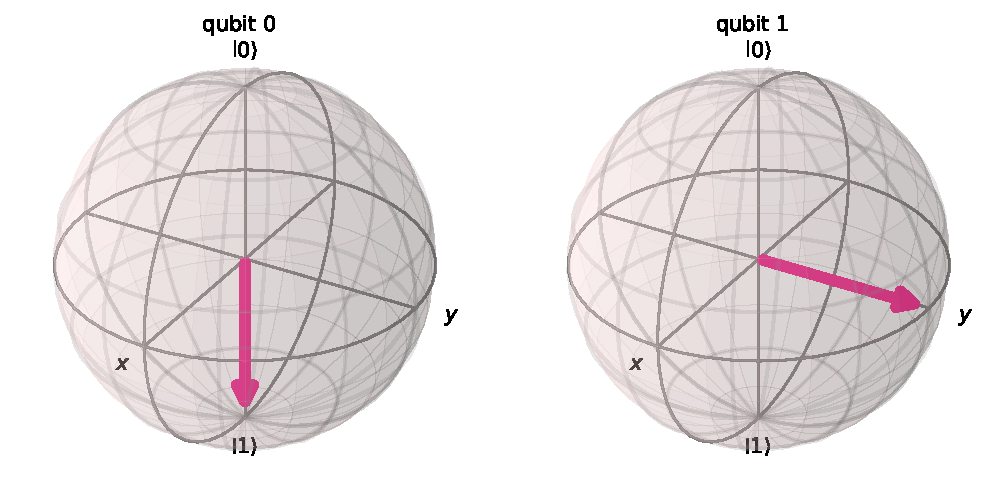
\includegraphics[keepaspectratio]{apostila_files/figure-pdf/cell-38-output-2.pdf}}

\begin{verbatim}

Amplitudes do estado final:
  |01⟩: amplitude = 0.7071, fase =    0.00°
  |11⟩: amplitude = 0.7071, fase =   90.00°
\end{verbatim}

\begin{verbatim}
Estado final (após CP) usando Qiskit:
\end{verbatim}

\begin{verbatim}

Amplitudes do estado final:
  |01⟩: amplitude = 0.7071, fase =    0.00°
  |11⟩: amplitude = 0.7071, fase =   90.00°
\end{verbatim}

\subsubsection{📝 Resumo: Porta CP no
Qiskit}\label{resumo-porta-cp-no-qiskit}

\textbf{Sintaxe:}

\begin{Shaded}
\begin{Highlighting}[]
\NormalTok{qc.cp(theta, control\_qubit, target\_qubit)}
\end{Highlighting}
\end{Shaded}

\textbf{Parâmetros:} - \texttt{theta}: ângulo de fase em radianos -
\texttt{control\_qubit}: índice do qubit de controle -
\texttt{target\_qubit}: índice do qubit alvo

\textbf{Efeito:} - Se o qubit de controle estiver em \textbar1⟩,
adiciona fase \texttt{e\^{}(iθ)} ao estado \textbar11⟩ - Se o qubit de
controle estiver em \textbar0⟩, nada acontece

\textbf{Casos especiais:} - \texttt{theta\ =\ π} → Porta CZ
(Controlled-Z) - \texttt{theta\ =\ π/2} → Porta CS (Controlled-S) -
\texttt{theta\ =\ π/4} → Porta CT (Controlled-T)

\subsubsection{Uso futuro da Porta CP}\label{uso-futuro-da-porta-cp}

Iremos entender a aplicação prática da porta CP em futuros notebooks,
especialmente quando discutirmos algoritmos quânticos que utilizam fases
para manipular estados quânticos de maneira eficiente. Mas, por
enquanto, é importante compreender a definição e o funcionamento básico
dessa porta quântica controlada, onde a fase do qubit alvo é alterada
dependendo do estado do qubit de controle.

\newpage

\chapter{Módulo 6: Circuitos, Estados de Bell e
Emaranhamento}\label{muxf3dulo-6-circuitos-estados-de-bell-e-emaranhamento}

\chapter{Aula 06 --- Primeiros Circuitos, Estados de Bell e
Emaranhamento}\label{aula-06-primeiros-circuitos-estados-de-bell-e-emaranhamento}

\chapter{🚀 Introdução ao Qiskit}\label{introduuxe7uxe3o-ao-qiskit}

Este notebook demonstra os conceitos fundamentais de programação
quântica usando o Qiskit.

\section{📚 O que vamos aprender}\label{o-que-vamos-aprender}

\begin{enumerate}
\def\labelenumi{\arabic{enumi}.}
\tightlist
\item
  Criar circuitos quânticos
\item
  Aplicar portas quânticas (H, CNOT, medições)
\item
  Executar simulações
\item
  Visualizar resultados
\item
  Entender a Esfera de Bloch
\end{enumerate}

\section{🔧 Bibliotecas Necessárias}\label{bibliotecas-necessuxe1rias}

Primeiro, vamos importar as bibliotecas que usaremos:

\begin{Shaded}
\begin{Highlighting}[]
\ImportTok{from}\NormalTok{ qiskit }\ImportTok{import}\NormalTok{ QuantumCircuit, transpile}
\ImportTok{from}\NormalTok{ qiskit\_aer }\ImportTok{import}\NormalTok{ AerSimulator}
\ImportTok{from}\NormalTok{ qiskit.visualization }\ImportTok{import}\NormalTok{ plot\_histogram, plot\_bloch\_multivector, plot\_state\_qsphere}
\ImportTok{from}\NormalTok{ qiskit.quantum\_info }\ImportTok{import}\NormalTok{ Statevector}
\end{Highlighting}
\end{Shaded}

\section{1️⃣ Construindo um Circuito Quântico
Simples}\label{construindo-um-circuito-quuxe2ntico-simples}

Vamos criar nosso primeiro circuito quântico com \textbf{2 qubits} e
\textbf{2 bits clássicos} para armazenar os resultados das medições.

\subsection{O que faremos:}\label{o-que-faremos}

\begin{itemize}
\tightlist
\item
  Criar um estado de \textbf{superposição} usando a porta Hadamard (H)
\item
  Criar \textbf{emaranhamento} usando a porta CNOT
\item
  Medir os qubits para obter resultados
\end{itemize}

\subsection{Passo 1: Criar o circuito
base}\label{passo-1-criar-o-circuito-base}

\begin{Shaded}
\begin{Highlighting}[]
\CommentTok{\# 1. CONSTRUÇÃO DO CIRCUITO}
\CommentTok{\# Criamos um circuito com 2 Qubits e 2 Bits Clássicos (para guardar o resultado)}
\NormalTok{qc }\OperatorTok{=}\NormalTok{ QuantumCircuit(}\DecValTok{2}\NormalTok{, }\DecValTok{2}\NormalTok{)}

\CommentTok{\# Visualizar estado inicial}
\NormalTok{estado\_inicial }\OperatorTok{=}\NormalTok{ Statevector.from\_instruction(qc)}
\BuiltInTok{print}\NormalTok{(}\StringTok{"Estado inicial: |00⟩"}\NormalTok{)}
\BuiltInTok{print}\NormalTok{(estado\_inicial)}

\CommentTok{\# Desenha o circuito}
\BuiltInTok{print}\NormalTok{(}\StringTok{"}\CharTok{\textbackslash{}n}\StringTok{Circuito inicial:"}\NormalTok{)}
\NormalTok{qc.draw(}\StringTok{\textquotesingle{}mpl\textquotesingle{}}\NormalTok{)}

\CommentTok{\# É uma boa prática para quem está aprendendo sempre desenhar o circuito após cada modificação.}
\end{Highlighting}
\end{Shaded}

\begin{verbatim}
Estado inicial: |00⟩
Statevector([1.+0.j, 0.+0.j, 0.+0.j, 0.+0.j],
            dims=(2, 2))

Circuito inicial:
\end{verbatim}

\pandocbounded{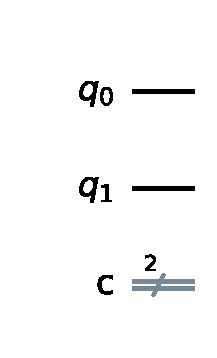
\includegraphics[keepaspectratio]{apostila_files/figure-pdf/cell-40-output-2.pdf}}

\begin{verbatim}
Estado inicial: |00⟩
Statevector([1.+0.j, 0.+0.j, 0.+0.j, 0.+0.j],
            dims=(2, 2))
\end{verbatim}

\begin{Shaded}
\begin{Highlighting}[]
\CommentTok{\# Esfera de Bloch {-} Estado inicial}
\NormalTok{plot\_bloch\_multivector(estado\_inicial)}
\end{Highlighting}
\end{Shaded}

\pandocbounded{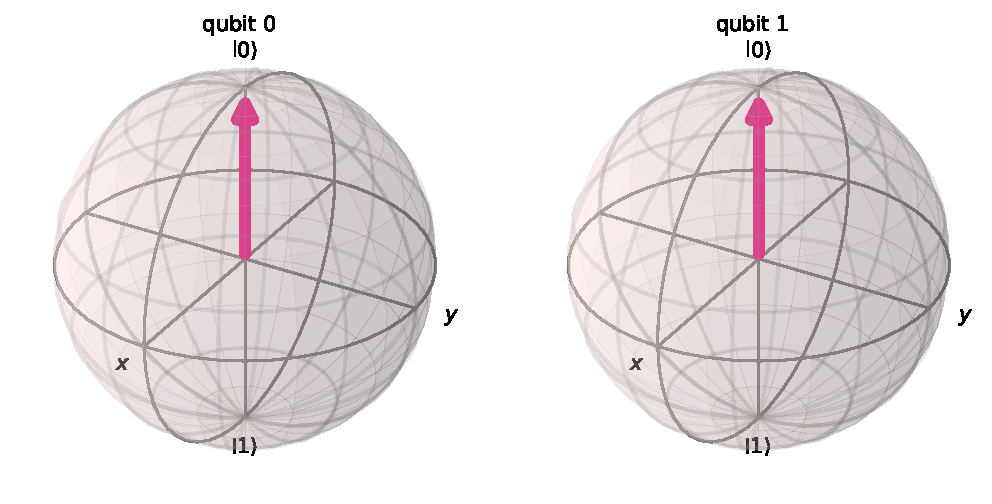
\includegraphics[keepaspectratio]{apostila_files/figure-pdf/cell-41-output-1.pdf}}

\subsection{Passo 2: Aplicar a Porta Hadamard
(H)}\label{passo-2-aplicar-a-porta-hadamard-h}

A porta Hadamard cria uma \textbf{superposição}: transforma \textbar0⟩
em um estado que é simultaneamente 0 e 1.

Matematicamente:
\[H|0\rangle = \frac{|0\rangle + |1\rangle}{\sqrt{2}} = |+\rangle\]

Isso significa 50\% de probabilidade de medir 0 e 50\% de medir 1.

\begin{Shaded}
\begin{Highlighting}[]
\CommentTok{\# Aplicamos a porta Hadamard (H) no qubit 0}
\CommentTok{\# Matematicamente: Leva |0\textgreater{} para uma superposição (50\% 0, 50\% 1)}
\NormalTok{qc.h(}\DecValTok{0}\NormalTok{)}

\CommentTok{\# Visualizar estado após Hadamard}
\NormalTok{estado\_apos\_h }\OperatorTok{=}\NormalTok{ Statevector.from\_instruction(qc)}
\BuiltInTok{print}\NormalTok{(}\StringTok{"Estado após H: 1/√2(|00⟩ + |10⟩)"}\NormalTok{)}
\BuiltInTok{print}\NormalTok{(estado\_apos\_h)}
\NormalTok{qc.draw(}\StringTok{\textquotesingle{}mpl\textquotesingle{}}\NormalTok{)}
\end{Highlighting}
\end{Shaded}

\begin{verbatim}
Estado após H: 1/√2(|00⟩ + |10⟩)
Statevector([0.70710678+0.j, 0.70710678+0.j, 0.        +0.j,
             0.        +0.j],
            dims=(2, 2))
\end{verbatim}

\pandocbounded{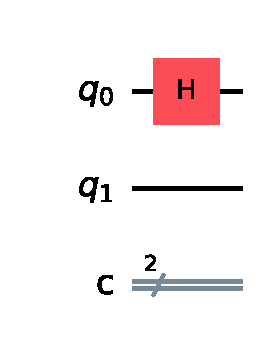
\includegraphics[keepaspectratio]{apostila_files/figure-pdf/cell-42-output-2.pdf}}

\begin{verbatim}
Estado após H: 1/√2(|00⟩ + |10⟩)
Statevector([0.70710678+0.j, 0.70710678+0.j, 0.        +0.j,
             0.        +0.j],
            dims=(2, 2))
\end{verbatim}

\begin{Shaded}
\begin{Highlighting}[]
\CommentTok{\# Esfera de Bloch {-} Após Hadamard}
\NormalTok{plot\_bloch\_multivector(estado\_apos\_h)}

\CommentTok{\# Veja que somente aplicamos a porta H no qubit 0, o qubit 1 permanece em |0⟩.}
\end{Highlighting}
\end{Shaded}

\pandocbounded{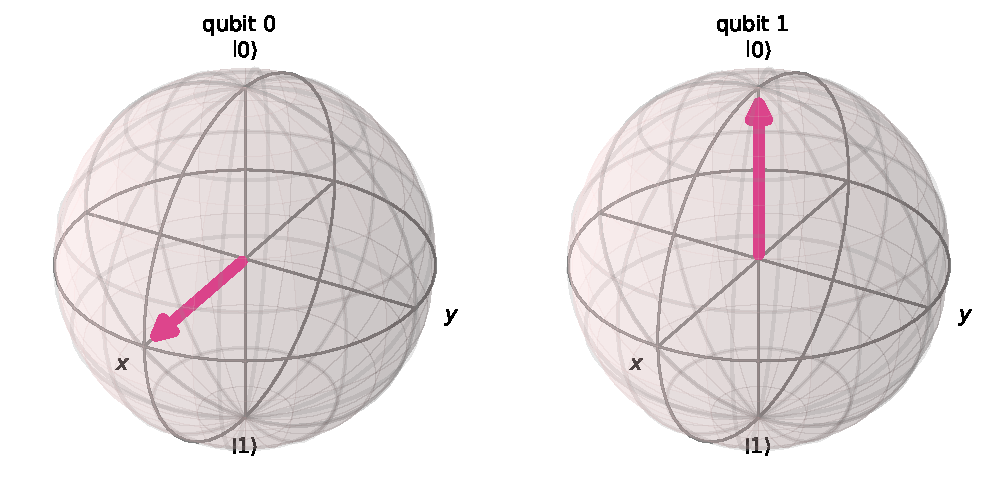
\includegraphics[keepaspectratio]{apostila_files/figure-pdf/cell-43-output-1.pdf}}

\subsection{Passo 3: Criar Emaranhamento com
CNOT}\label{passo-3-criar-emaranhamento-com-cnot}

A porta CNOT (Controlled-NOT) é uma porta de \textbf{dois qubits}: -
\textbf{Qubit 0} (controle): Se estiver em \textbar1⟩, inverte o qubit
alvo - \textbf{Qubit 1} (alvo): É invertido se o controle for \textbar1⟩

Como o qubit 0 está em superposição, isso cria \textbf{emaranhamento}
entre os dois qubits!

Matematicamente, criamos o estado de Bell:
\[|\Phi^+\rangle = \frac{|00\rangle + |11\rangle}{\sqrt{2}}\]

Isso significa: ou \textbf{ambos são 0}, ou \textbf{ambos são 1} - nunca
01 ou 10!

\begin{Shaded}
\begin{Highlighting}[]
\CommentTok{\# Aplicamos a porta CNOT (Control{-}NOT)}
\CommentTok{\# O Qubit 0 é o controle, o Qubit 1 é o alvo.}
\CommentTok{\# Se o Qubit 0 for 1, ele inverte o Qubit 1.}
\CommentTok{\# Como o Qubit 0 está em superposição, eles ficam EMARANHADOS.}
\NormalTok{qc.cx(}\DecValTok{0}\NormalTok{, }\DecValTok{1}\NormalTok{)}

\CommentTok{\# Visualizar estado após CNOT (Estado de Bell)}
\NormalTok{estado\_apos\_cnot }\OperatorTok{=}\NormalTok{ Statevector.from\_instruction(qc)}
\BuiltInTok{print}\NormalTok{(}\StringTok{"Estado após CNOT: 1/√2(|00⟩ + |11⟩) {-} Estado de Bell |Φ+⟩"}\NormalTok{)}
\BuiltInTok{print}\NormalTok{(estado\_apos\_cnot)}
\NormalTok{qc.draw(}\StringTok{\textquotesingle{}mpl\textquotesingle{}}\NormalTok{)}
\end{Highlighting}
\end{Shaded}

\begin{verbatim}
Estado após CNOT: 1/√2(|00⟩ + |11⟩) - Estado de Bell |Φ+⟩
Statevector([0.70710678+0.j, 0.        +0.j, 0.        +0.j,
             0.70710678+0.j],
            dims=(2, 2))
\end{verbatim}

\pandocbounded{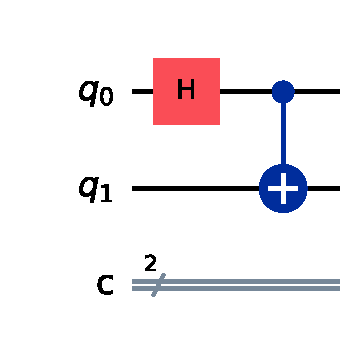
\includegraphics[keepaspectratio]{apostila_files/figure-pdf/cell-44-output-2.pdf}}

\begin{verbatim}
Estado após CNOT: 1/√2(|00⟩ + |11⟩) - Estado de Bell |Φ+⟩
Statevector([0.70710678+0.j, 0.        +0.j, 0.        +0.j,
             0.70710678+0.j],
            dims=(2, 2))
\end{verbatim}

\begin{Shaded}
\begin{Highlighting}[]
\CommentTok{\# Q{-}Sphere {-} Melhor para visualizar o estado emaranhado completo}
\BuiltInTok{print}\NormalTok{(}\StringTok{"}\CharTok{\textbackslash{}n}\StringTok{🌐 Q{-}Sphere {-} Mostra todas as amplitudes do estado emaranhado:"}\NormalTok{)}
\NormalTok{plot\_state\_qsphere(estado\_apos\_cnot)}
\end{Highlighting}
\end{Shaded}

\begin{verbatim}

🌐 Q-Sphere - Mostra todas as amplitudes do estado emaranhado:
\end{verbatim}

\pandocbounded{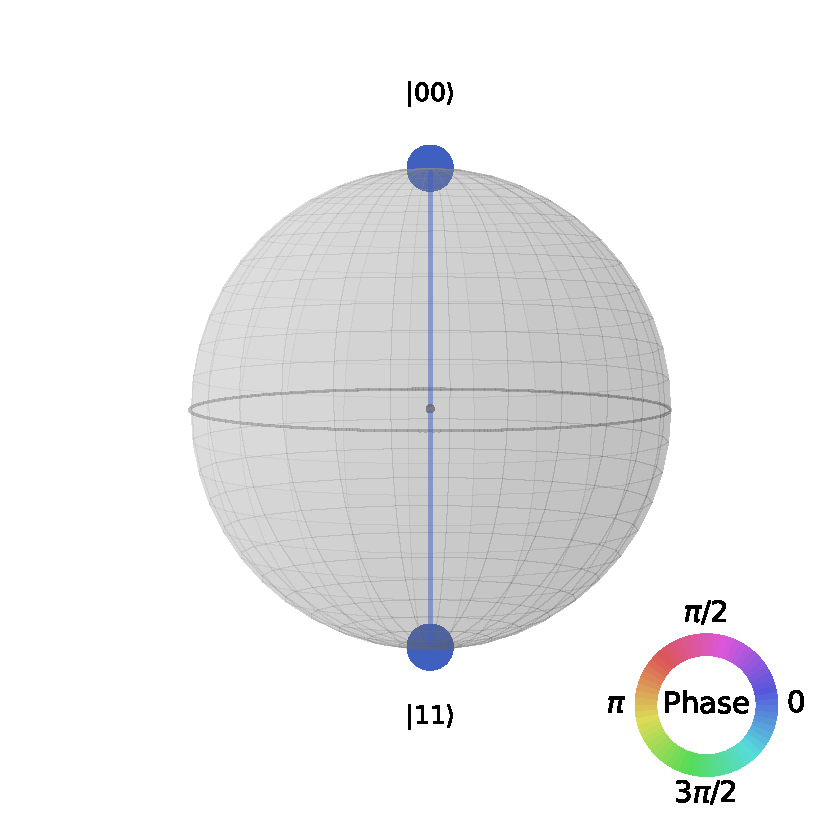
\includegraphics[keepaspectratio]{apostila_files/figure-pdf/cell-45-output-2.pdf}}

\begin{verbatim}

🌐 Q-Sphere - Mostra todas as amplitudes do estado emaranhado:
\end{verbatim}

\subsection{Passo 4: Medir os Qubits}\label{passo-4-medir-os-qubits}

A medição \textbf{colapsa} o estado quântico para um resultado clássico:
- Qubit 0 → armazena no bit clássico 0 - Qubit 1 → armazena no bit
clássico 1

Após a medição, teremos apenas 0s e 1s (não mais superposição).

\begin{Shaded}
\begin{Highlighting}[]
\CommentTok{\# Medimos os qubits}
\CommentTok{\# Qubit 0 {-}\textgreater{} guarda no Bit 0}
\CommentTok{\# Qubit 1 {-}\textgreater{} guarda no Bit 1}
\NormalTok{qc.measure([}\DecValTok{0}\NormalTok{, }\DecValTok{1}\NormalTok{], [}\DecValTok{0}\NormalTok{, }\DecValTok{1}\NormalTok{])}

\CommentTok{\# Desenhar circuito completo}
\NormalTok{qc.draw(}\StringTok{\textquotesingle{}mpl\textquotesingle{}}\NormalTok{)}
\end{Highlighting}
\end{Shaded}

\pandocbounded{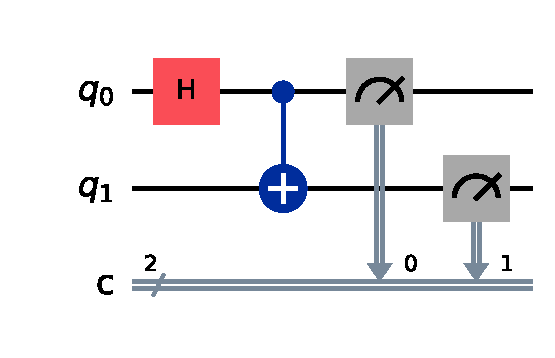
\includegraphics[keepaspectratio]{apostila_files/figure-pdf/cell-46-output-1.pdf}}

⚠️ \textbf{Nota:} Após adicionar as medições, não podemos mais extrair o
Statevector (a medição colapsa o estado). As visualizações acima mostram
o estado \textbf{antes} da medição.

\section{2️⃣ Executando o Circuito
(Simulação)}\label{executando-o-circuito-simulauxe7uxe3o}

Agora vamos \textbf{executar} o circuito usando um simulador quântico.
Rodaremos 1000 vezes para ver a distribuição de probabilidades.

\subsection{Processo:}\label{processo}

\begin{enumerate}
\def\labelenumi{\arabic{enumi}.}
\tightlist
\item
  \textbf{Transpilação}: Otimiza o circuito para o simulador
\item
  \textbf{Execução}: Roda 1000 vezes (shots)
\item
  \textbf{Análise}: Coleta os resultados estatísticos
\end{enumerate}

\begin{Shaded}
\begin{Highlighting}[]
\CommentTok{\# 2. EXECUÇÃO (SIMULAÇÃO)}
\NormalTok{simulador }\OperatorTok{=}\NormalTok{ AerSimulator()}

\CommentTok{\# Transpilação: otimiza o circuito para o backend específico (neste caso, o simulador)}
\NormalTok{circuito\_compilado }\OperatorTok{=}\NormalTok{ transpile(qc, simulador)}

\CommentTok{\# Rodamos a simulação 1000 vezes (shots)}
\NormalTok{job }\OperatorTok{=}\NormalTok{ simulador.run(circuito\_compilado, shots}\OperatorTok{=}\DecValTok{1000}\NormalTok{)}

\CommentTok{\# 3. ANÁLISE DE RESULTADOS}
\NormalTok{resultado }\OperatorTok{=}\NormalTok{ job.result()}
\NormalTok{contagens }\OperatorTok{=}\NormalTok{ resultado.get\_counts()}

\BuiltInTok{print}\NormalTok{(}\StringTok{"}\CharTok{\textbackslash{}n}\StringTok{{-}{-}{-} Resultados da Medição (1000 execuções) {-}{-}{-}"}\NormalTok{)}
\BuiltInTok{print}\NormalTok{(contagens)}
\end{Highlighting}
\end{Shaded}

\begin{verbatim}

--- Resultados da Medição (1000 execuções) ---
{'00': 490, '11': 510}
\end{verbatim}

\begin{verbatim}

--- Resultados da Medição (1000 execuções) ---
{'00': 503, '11': 497}
\end{verbatim}

\subsection{📊 Interpretando os
Resultados}\label{interpretando-os-resultados}

Observe os resultados acima - você verá apenas \textbf{00} e
\textbf{11}, aproximadamente 50\% cada.

\textbf{Por quê?} - O qubit 0 estava em superposição (era 0 e 1 ao mesmo
tempo) - O qubit 1 começou em 0 - Quando aplicamos CNOT, criamos
\textbf{emaranhamento}: ou ambos são 0, ou ambos são 1

\textbf{Importante:} Não existe probabilidade de obter 01 ou 10! Isso é
a ``magia'' do emaranhamento quântico.

\subsection{🎯 O Estado de Bell}\label{o-estado-de-bell}

Matematicamente, criamos o famoso \textbf{estado de Bell}:

\[|\Phi^+\rangle = \frac{|00\rangle + |11\rangle}{\sqrt{2}}\]

Este é um dos estados mais importantes da computação quântica!

\textbf{Significado:} - É uma correlação que \textbf{não existe na
física clássica} - Base para teletransporte quântico, criptografia
quântica e outros protocolos - Demonstra o poder único dos computadores
quânticos

\section{3️⃣ Visualização Avançada: A Esfera de
Bloch}\label{visualizauxe7uxe3o-avanuxe7ada-a-esfera-de-bloch}

\subsection{🌍 O Conceito: Navegando na
Esfera}\label{o-conceito-navegando-na-esfera}

A \textbf{Esfera de Bloch} é uma representação geométrica 3D do estado
de um qubit.

Imagine o planeta Terra:

\begin{itemize}
\tightlist
\item
  \textbf{Pólo Norte ⬆️}: Estado \textbar0⟩
\item
  \textbf{Pólo Sul ⬇️}: Estado \textbar1⟩
\item
  \textbf{Equador 🌍}: Estados de \textbf{superposição} (50\% de chance
  de 0 ou 1)
\end{itemize}

O vetor de estado é uma \textbf{seta} do centro da esfera até a
superfície: - Apontando para cima → qubit é \textbar0⟩ - Apontando para
baixo → qubit é \textbar1⟩ - Apontando para o equador → qubit em
superposição

\subsection{📐 Matemática da Esfera}\label{matemuxe1tica-da-esfera}

O estado geral de um qubit pode ser escrito como:
\[|\psi\rangle = \cos\left(\frac{\theta}{2}\right)|0\rangle + e^{i\phi}\sin\left(\frac{\theta}{2}\right)|1\rangle\]

Onde: - \textbf{θ (theta)}: Ângulo polar - controla probabilidade de 0
vs 1 (latitude) - \textbf{φ (phi)}: Ângulo azimutal - controla a fase
quântica (longitude)

\textbf{Importante:} A fase φ não afeta a probabilidade de medição, mas
é crucial para \textbf{interferência quântica} em algoritmos!

\subsection{💡 Exemplos Práticos}\label{exemplos-pruxe1ticos}

Vamos visualizar três estados fundamentais na Esfera de Bloch:

\begin{Shaded}
\begin{Highlighting}[]
\OperatorTok{\%}\NormalTok{matplotlib inline}

\CommentTok{\# {-}{-}{-} 1. Estado Inicial (|0\textgreater{}) {-}{-}{-}}
\CommentTok{\# Um circuito vazio começa sempre em zero}
\NormalTok{qc\_zero }\OperatorTok{=}\NormalTok{ QuantumCircuit(}\DecValTok{1}\NormalTok{)}

\CommentTok{\# Extraímos o estado matemático (vetor)}
\NormalTok{estado\_zero }\OperatorTok{=}\NormalTok{ Statevector(qc\_zero)}

\BuiltInTok{print}\NormalTok{(}\StringTok{"Gerando imagem do Estado Zero (Pólo Norte)..."}\NormalTok{)}

\CommentTok{\# Nota: plot\_bloch\_multivector retorna uma figura matplotlib}
\NormalTok{fig1 }\OperatorTok{=}\NormalTok{ plot\_bloch\_multivector(estado\_zero, title}\OperatorTok{=}\StringTok{"Estado Inicial |0\textgreater{}"}\NormalTok{)}
\end{Highlighting}
\end{Shaded}

\begin{verbatim}
Gerando imagem do Estado Zero (Pólo Norte)...
\end{verbatim}

\pandocbounded{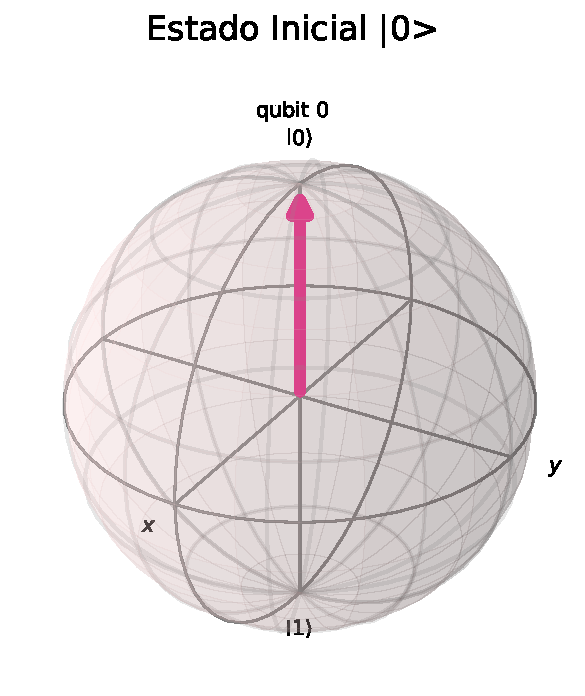
\includegraphics[keepaspectratio]{apostila_files/figure-pdf/cell-48-output-2.pdf}}

\begin{verbatim}
Gerando imagem do Estado Zero (Pólo Norte)...
\end{verbatim}

\subsubsection{Exemplo 1: Estado Inicial \textbar0⟩ (Pólo
Norte)}\label{exemplo-1-estado-inicial-0-puxf3lo-norte}

Um circuito vazio sempre começa com todos os qubits em \textbar0⟩:

\begin{Shaded}
\begin{Highlighting}[]
\CommentTok{\# {-}{-}{-} 2. Estado de Superposição (Apicando Hadamard) {-}{-}{-}}
\NormalTok{qc\_super }\OperatorTok{=}\NormalTok{ QuantumCircuit(}\DecValTok{1}\NormalTok{)}
\NormalTok{qc\_super.h(}\DecValTok{0}\NormalTok{) }\CommentTok{\# Aplica H}
\CommentTok{\# qc\_super.z(0) \# Aplica Z para mostrar diferença de fase}
\NormalTok{estado\_super }\OperatorTok{=}\NormalTok{ Statevector(qc\_super)}

\BuiltInTok{print}\NormalTok{(}\StringTok{"Gerando imagem da Superposição (Equador)..."}\NormalTok{)}
\NormalTok{fig2 }\OperatorTok{=}\NormalTok{ plot\_bloch\_multivector(estado\_super, title}\OperatorTok{=}\StringTok{"Após Hadamard |+\textgreater{}"}\NormalTok{)}
\end{Highlighting}
\end{Shaded}

\begin{verbatim}
Gerando imagem da Superposição (Equador)...
\end{verbatim}

\pandocbounded{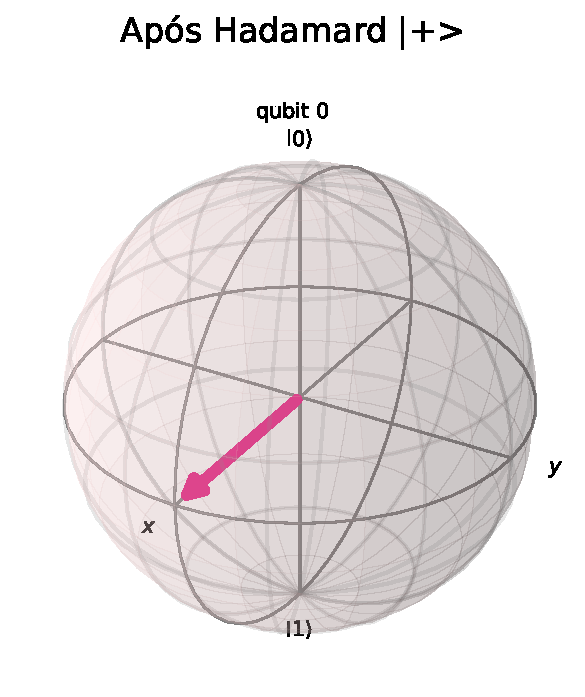
\includegraphics[keepaspectratio]{apostila_files/figure-pdf/cell-49-output-2.pdf}}

\begin{verbatim}
Gerando imagem da Superposição (Equador)...
\end{verbatim}

\subsubsection{Exemplo 2: Superposição \textbar+⟩
(Equador)}\label{exemplo-2-superposiuxe7uxe3o-equador}

Aplicando a porta Hadamard, movemos o estado do pólo norte para o
equador:

\begin{Shaded}
\begin{Highlighting}[]
\CommentTok{\# {-}{-}{-} 3. Estado Invertido (Aplicando X) {-}{-}{-}}
\NormalTok{qc\_inv }\OperatorTok{=}\NormalTok{ QuantumCircuit(}\DecValTok{1}\NormalTok{)}
\NormalTok{qc\_inv.x(}\DecValTok{0}\NormalTok{) }\CommentTok{\# Aplica X}
\NormalTok{estado\_inv }\OperatorTok{=}\NormalTok{ Statevector(qc\_inv)}

\BuiltInTok{print}\NormalTok{(}\StringTok{"Gerando imagem do Estado Invertido (Pólo Sul)..."}\NormalTok{)}
\NormalTok{fig3 }\OperatorTok{=}\NormalTok{ plot\_bloch\_multivector(estado\_inv, title}\OperatorTok{=}\StringTok{"Após Porta X |1\textgreater{}"}\NormalTok{)}
\end{Highlighting}
\end{Shaded}

\begin{verbatim}
Gerando imagem do Estado Invertido (Pólo Sul)...
\end{verbatim}

\pandocbounded{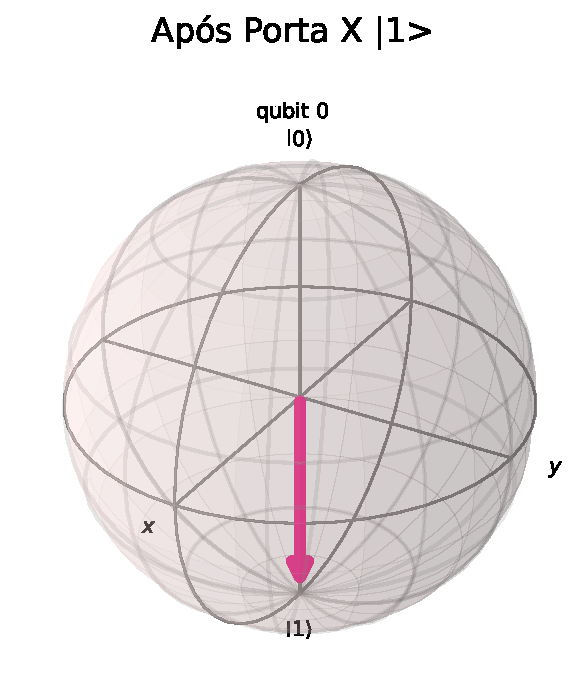
\includegraphics[keepaspectratio]{apostila_files/figure-pdf/cell-50-output-2.pdf}}

\begin{verbatim}
Gerando imagem do Estado Invertido (Pólo Sul)...
\end{verbatim}

\subsubsection{Exemplo 3: Estado \textbar1⟩ (Pólo
Sul)}\label{exemplo-3-estado-1-puxf3lo-sul}

Aplicando a porta X (NOT quântico), invertemos completamente o estado:

\subsection{📊 Interpretando as
Visualizações}\label{interpretando-as-visualizauxe7uxf5es}

O que você verá nas figuras acima:

\begin{enumerate}
\def\labelenumi{\arabic{enumi}.}
\tightlist
\item
  \textbf{Figura 1 (Estado Inicial):}

  \begin{itemize}
  \tightlist
  \item
    A seta vermelha aponta para o \textbf{Pólo Norte (Eixo Z+)}
  \item
    Isso é o estado \textbar0⟩
  \item
    100\% de probabilidade de medir 0
  \end{itemize}
\item
  \textbf{Figura 2 (Após Hadamard):}

  \begin{itemize}
  \tightlist
  \item
    A seta desce para o \textbf{Equador (Eixo X+)}
  \item
    Estado \textbar+⟩ = superposição com fase positiva
  \item
    50\% de chance de medir 0, 50\% de medir 1
  \item
    A direção específica (X+) indica a \textbf{fase} da superposição
  \end{itemize}
\item
  \textbf{Figura 3 (Após Porta X):}

  \begin{itemize}
  \tightlist
  \item
    A seta aponta para o \textbf{Pólo Sul (Eixo Z-)}
  \item
    Isso é o estado \textbar1⟩
  \item
    100\% de probabilidade de medir 1
  \end{itemize}
\end{enumerate}

\subsection{🎯 Entendendo a Fase
Quântica}\label{entendendo-a-fase-quuxe2ntica}

\textbf{Experimento:} Tente adicionar uma porta Z logo após a porta H na
Exemplo 2:

\begin{Shaded}
\begin{Highlighting}[]
\NormalTok{qc\_super.h(}\DecValTok{0}\NormalTok{)  }\CommentTok{\# Hadamard}
\NormalTok{qc\_super.z(}\DecValTok{0}\NormalTok{)  }\CommentTok{\# Porta Z {-} rotação de fase}
\end{Highlighting}
\end{Shaded}

A porta Z \textbf{gira o qubit ao redor do eixo vertical} (eixo Z).

\textbf{O que acontece:} - \textbf{Visualmente:} A seta continua no
equador (mesma probabilidade 50/50) - \textbf{Mas:} Agora aponta para
\textbf{Eixo X-} (fase negativa) - \textbf{Significado:} A probabilidade
não muda, mas a \textbf{fase} muda!

\textbf{Por que isso importa:} - Em algoritmos quânticos, qubits
interferem uns com os outros - A direção da seta (fase) determina se a
interferência será \textbf{construtiva} ou \textbf{destrutiva} - Isso é
fundamental para algoritmos como Grover e Shor!

\section{🎓 Resumo do que Aprendemos}\label{resumo-do-que-aprendemos}

Parabéns! Você já dominou os fundamentos:

\subsection{✅ Conceitos Matemáticos}\label{conceitos-matemuxe1ticos}

\begin{itemize}
\tightlist
\item
  Vetores de estado representam qubits
\item
  Matrizes representam portas quânticas
\item
  Superposição e emaranhamento como operações lineares
\end{itemize}

\subsection{✅ Programação no Qiskit}\label{programauxe7uxe3o-no-qiskit}

\begin{itemize}
\tightlist
\item
  Criar circuitos quânticos (\texttt{QuantumCircuit})
\item
  Aplicar portas (H, X, CNOT)
\item
  Medir qubits
\item
  Executar simulações
\end{itemize}

\subsection{✅ Visualização}\label{visualizauxe7uxe3o}

\begin{itemize}
\tightlist
\item
  Entender a Esfera de Bloch
\item
  Interpretar o vetor de estado geometricamente
\item
  Distinguir probabilidade vs fase quântica
\end{itemize}

\subsection{🚀 Próximos Passos}\label{pruxf3ximos-passos}

Agora você está pronto para explorar: - Algoritmos quânticos
(Deutsch-Jozsa, Grover, Shor) - Protocolos de comunicação quântica
(Teletransporte, Superdense Coding) - Correção de erros quânticos -
Computação quântica em hardware real (IBM Quantum)

\newpage

\chapter{Módulo 7: Teletransporte
Quântico}\label{muxf3dulo-7-teletransporte-quuxe2ntico}

\chapter{Aula 07 --- Protocolo de Teletransporte
Quântico}\label{aula-07-protocolo-de-teletransporte-quuxe2ntico}

\chapter{🚀 Teletransporte Quântico - como Star Trek, mas
real!}\label{teletransporte-quuxe2ntico---como-star-trek-mas-real}

\section{💡 A Ideia Básica}\label{a-ideia-buxe1sica}

Imagine que Alice quer enviar uma informação quântica para Bob que está
muito longe.

\textbf{Analogia:} É como enviar uma foto pelo celular, mas para
informação quântica: - Alice não pode simplesmente ``copiar'' o estado
quântico (lei da mecânica quântica!) - Mas se Alice e Bob compartilharem
algo especial (emaranhamento), ela pode \textbf{transferir} o estado - O
estado original de Alice é destruído no processo

\section{👥 Os Personagens}\label{os-personagens}

\begin{itemize}
\tightlist
\item
  \textbf{Alice} 👩: Tem um qubit misterioso (qubit 0) que quer
  teletransportar
\item
  \textbf{Bob} 🧑: Vai receber o estado no seu qubit (qubit 2)
\item
  \textbf{Par Emaranhado} ✨: Qubits 1 e 2 conectados quanticamente
\end{itemize}

\section{📋 Os 5 Passos do
Teletransporte}\label{os-5-passos-do-teletransporte}

\begin{enumerate}
\def\labelenumi{\arabic{enumi}.}
\tightlist
\item
  ✅ Criar o circuito
\item
  🎯 Alice prepara seu qubit misterioso\\
\item
  ⚡ Criar emaranhamento + medição de Bell
\item
  📞 Alice mede e ``liga'' para Bob
\item
  🔧 Bob faz correções e recebe o estado!
\end{enumerate}

\section{Passo 0: Importar
bibliotecas}\label{passo-0-importar-bibliotecas}

\begin{Shaded}
\begin{Highlighting}[]
\ImportTok{from}\NormalTok{ qiskit }\ImportTok{import}\NormalTok{ QuantumRegister, ClassicalRegister, QuantumCircuit}
\ImportTok{from}\NormalTok{ qiskit.quantum\_info }\ImportTok{import}\NormalTok{ Statevector}
\ImportTok{from}\NormalTok{ qiskit.visualization }\ImportTok{import}\NormalTok{ plot\_bloch\_multivector, plot\_state\_qsphere, plot\_state\_city}
\ImportTok{from}\NormalTok{ numpy }\ImportTok{import}\NormalTok{ pi}
\end{Highlighting}
\end{Shaded}

\section{1️⃣ Passo 1: Montar o ``Palco'' do
Teletransporte}\label{passo-1-montar-o-palco-do-teletransporte}

Vamos criar nosso circuito quântico - o ``palco'' onde tudo vai
acontecer.

\textbf{O que precisamos:}

\begin{itemize}
\item
  \textbf{3 qubits} (q{[}0{]}, q{[}1{]}, q{[}2{]}) - nossos ``atores''
  quânticos💡 \textbf{Pense como:} 3 moedas quânticas e 3 caixinhas para
  guardar resultados

  \begin{itemize}
  \item
    q{[}0{]}: Qubit de Alice (o que será teletransportado)
  \item
    q{[}1{]}: Metade do par emaranhado que fica com Alice
  \item
    q{[}2{]}: Metade do par emaranhado que fica com Bob
  \item
    \textbf{3 bits clássicos} (c{[}0{]}, c{[}1{]}, c{[}2{]}) - para
    guardar resultados das medições
  \end{itemize}
\end{itemize}

\subsection{📐 Estado Matemático
Inicial}\label{estado-matemuxe1tico-inicial}

No início, todos os qubits estão em \(|0\rangle\):

\[|\psi_{\text{inicial}}\rangle = |q_0\rangle \otimes |q_1\rangle \otimes |q_2\rangle = |0\rangle \otimes |0\rangle \otimes |0\rangle = |000\rangle\]

\begin{Shaded}
\begin{Highlighting}[]
\NormalTok{qreg\_q }\OperatorTok{=}\NormalTok{ QuantumRegister(}\DecValTok{3}\NormalTok{, }\StringTok{\textquotesingle{}q\textquotesingle{}}\NormalTok{)}
\NormalTok{creg\_c }\OperatorTok{=}\NormalTok{ ClassicalRegister(}\DecValTok{3}\NormalTok{, }\StringTok{\textquotesingle{}c\textquotesingle{}}\NormalTok{)}
\NormalTok{circuit }\OperatorTok{=}\NormalTok{ QuantumCircuit(qreg\_q, creg\_c)}
\NormalTok{circuit.draw(}\StringTok{\textquotesingle{}mpl\textquotesingle{}}\NormalTok{)}

\NormalTok{state1 }\OperatorTok{=}\NormalTok{ Statevector.from\_instruction(circuit)}
\BuiltInTok{print}\NormalTok{(state1)}
\NormalTok{plot\_bloch\_multivector(state1)}
\end{Highlighting}
\end{Shaded}

\begin{verbatim}
Statevector([1.+0.j, 0.+0.j, 0.+0.j, 0.+0.j, 0.+0.j, 0.+0.j, 0.+0.j,
             0.+0.j],
            dims=(2, 2, 2))
\end{verbatim}

\pandocbounded{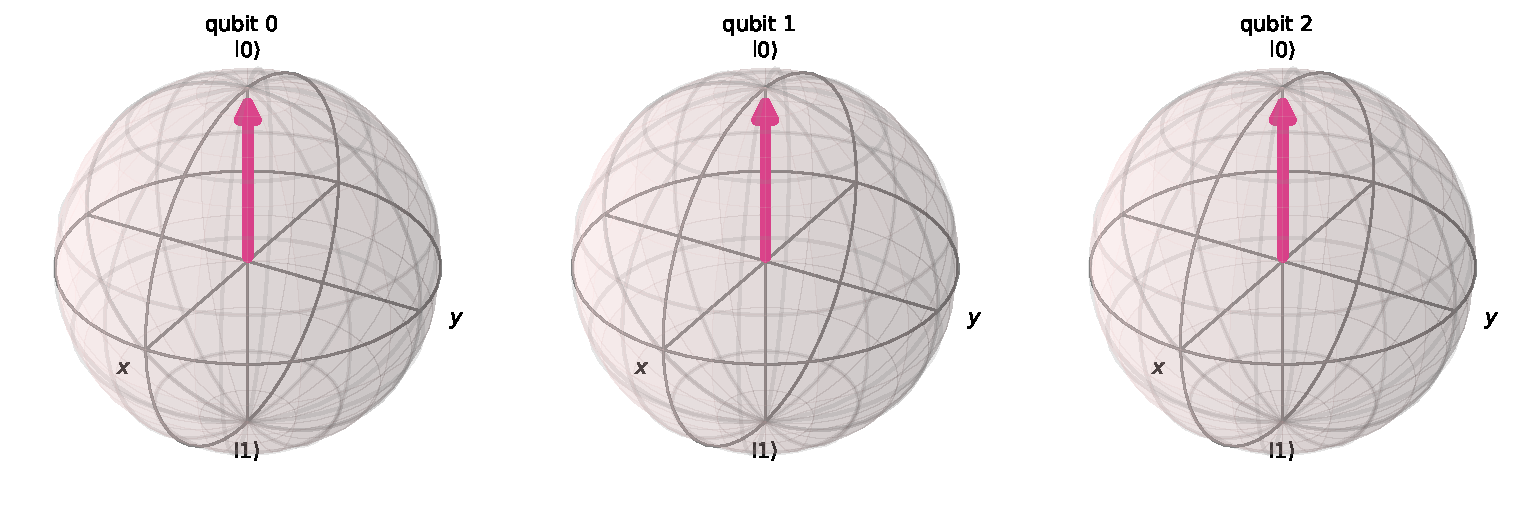
\includegraphics[keepaspectratio]{apostila_files/figure-pdf/cell-52-output-2.pdf}}

\pandocbounded{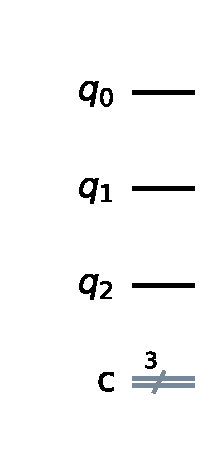
\includegraphics[keepaspectratio]{apostila_files/figure-pdf/cell-52-output-3.pdf}}

\pandocbounded{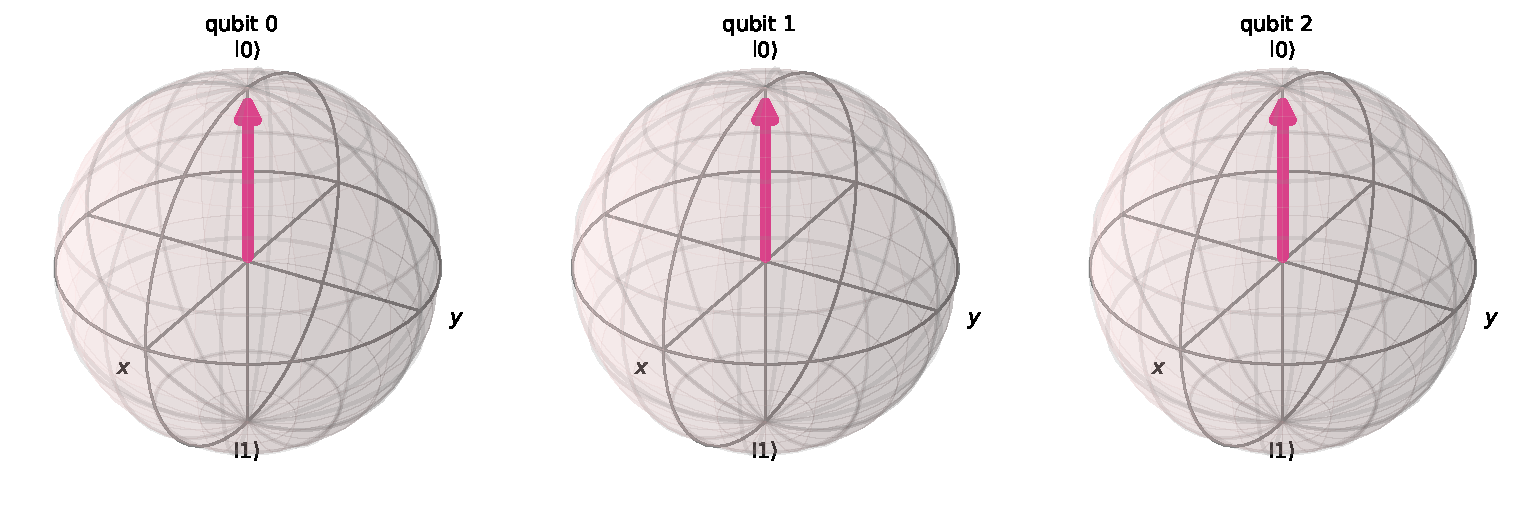
\includegraphics[keepaspectratio]{apostila_files/figure-pdf/cell-52-output-4.pdf}}

\begin{verbatim}
Statevector([1.+0.j, 0.+0.j, 0.+0.j, 0.+0.j, 0.+0.j, 0.+0.j, 0.+0.j,
             0.+0.j],
            dims=(2, 2, 2))
\end{verbatim}

\section{2️⃣ Passo 2: Alice Prepara o ``Pacote'' a
Enviar}\label{passo-2-alice-prepara-o-pacote-a-enviar}

\textbf{Alice} cria o estado que quer teletransportar no qubit 0.

🎁 \textbf{O que estamos enviando:} Estado \textbar1⟩ (usando porta X)

🚧 \textbf{Barreira:} Separamos visualmente as etapas do circuito

💭 \textbf{Por que \textbar1⟩?} Para facilitar a verificação! No final,
se Bob receber \textbar1⟩, sabemos que funcionou.

⚡ \textbf{Na vida real:} Poderia ser qualquer estado quântico
\textbar ψ⟩ = α\textbar0⟩ + β\textbar1⟩, mesmo que Alice não saiba os
valores de α e β!

\subsection{📐 Cálculo da Porta X}\label{cuxe1lculo-da-porta-x}

A porta X (NOT quântico) transforma:

\[X|0\rangle = |1\rangle\]

Matematicamente, a porta X é representada pela matriz de Pauli:

\[X = \begin{pmatrix} 0 & 1 \\ 1 & 0 \end{pmatrix}\]

Aplicando no qubit 0:

\[|\psi_1\rangle = (X \otimes I \otimes I)|000\rangle = |100\rangle = |1\rangle \otimes |0\rangle \otimes |0\rangle\]

\begin{Shaded}
\begin{Highlighting}[]
\NormalTok{circuit.x(qreg\_q[}\DecValTok{0}\NormalTok{])}
\NormalTok{circuit.barrier(qreg\_q[}\DecValTok{0}\NormalTok{], qreg\_q[}\DecValTok{1}\NormalTok{], qreg\_q[}\DecValTok{2}\NormalTok{])}

\NormalTok{circuit.draw(}\StringTok{\textquotesingle{}mpl\textquotesingle{}}\NormalTok{)}
\NormalTok{state2 }\OperatorTok{=}\NormalTok{ Statevector.from\_instruction(circuit)}
\BuiltInTok{print}\NormalTok{(state2)}
\NormalTok{plot\_bloch\_multivector(state2)}
\end{Highlighting}
\end{Shaded}

\begin{verbatim}
Statevector([0.+0.j, 1.+0.j, 0.+0.j, 0.+0.j, 0.+0.j, 0.+0.j, 0.+0.j,
             0.+0.j],
            dims=(2, 2, 2))
\end{verbatim}

\pandocbounded{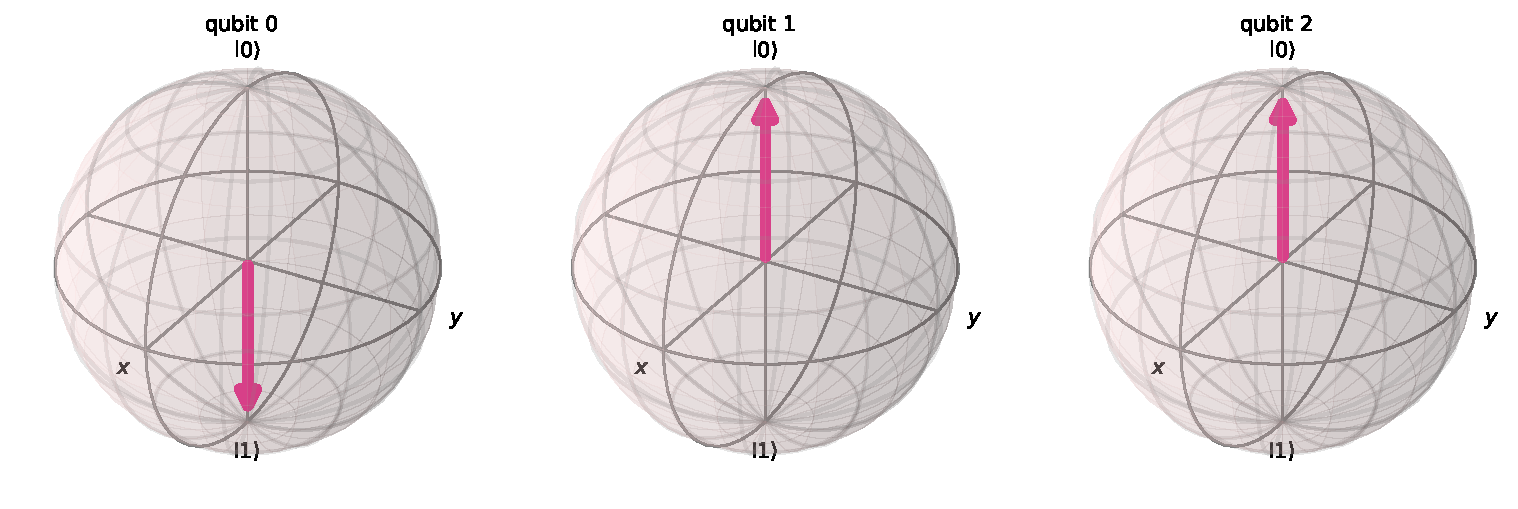
\includegraphics[keepaspectratio]{apostila_files/figure-pdf/cell-53-output-2.pdf}}

\pandocbounded{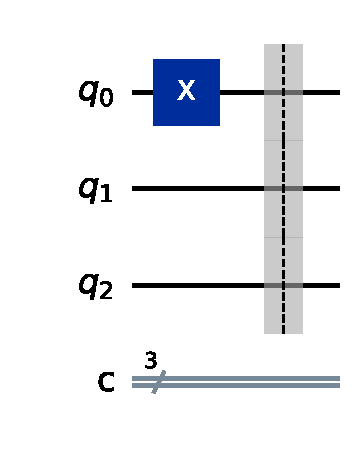
\includegraphics[keepaspectratio]{apostila_files/figure-pdf/cell-53-output-3.pdf}}

\pandocbounded{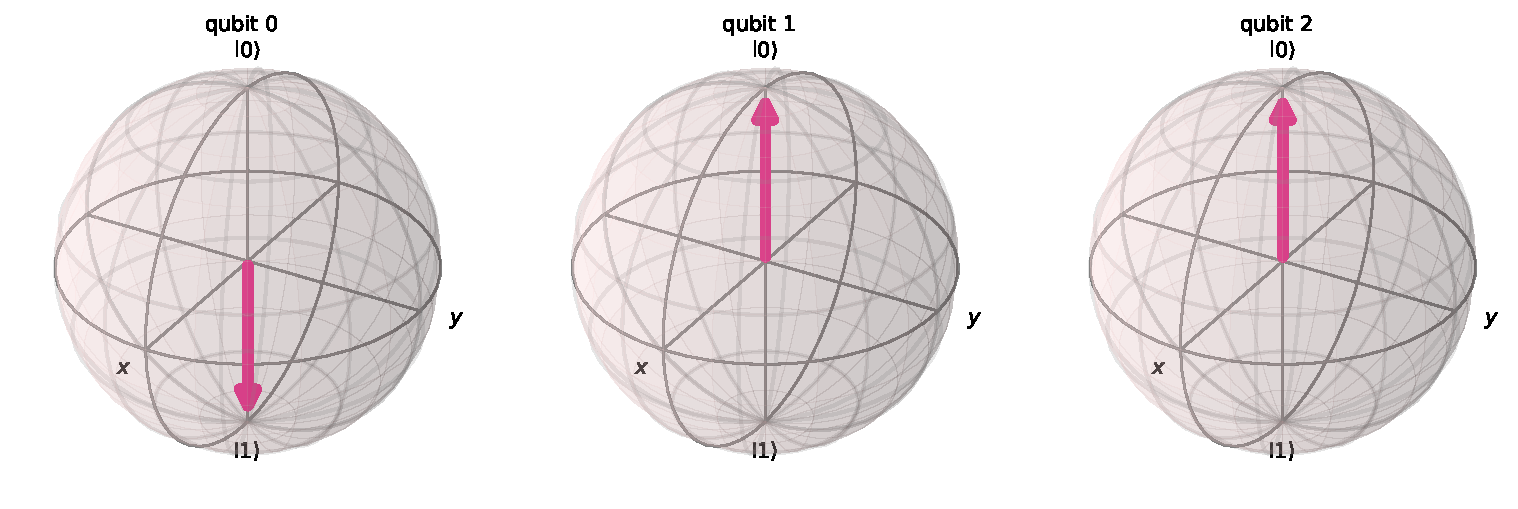
\includegraphics[keepaspectratio]{apostila_files/figure-pdf/cell-53-output-4.pdf}}

\begin{verbatim}
Statevector([0.+0.j, 1.+0.j, 0.+0.j, 0.+0.j, 0.+0.j, 0.+0.j, 0.+0.j,
             0.+0.j],
            dims=(2, 2, 2))
\end{verbatim}

\section{3️⃣ Passo 3: A Mágica Quântica -
Emaranhamento!}\label{passo-3-a-muxe1gica-quuxe2ntica---emaranhamento}

Esta é a parte mais importante! Aqui acontece a ``conexão mágica'' entre
Alice e Bob.

\subsection{🔗 Parte A: Criar o ``Telefone Quântico'' (Par de
Bell)}\label{parte-a-criar-o-telefone-quuxe2ntico-par-de-bell}

Alice e Bob precisam ter compartilhado um par de qubits emaranhados
antes:

\begin{enumerate}
\def\labelenumi{\arabic{enumi}.}
\tightlist
\item
  \textbf{H(q{[}1{]})} - Porta Hadamard: Coloca qubit 1 em superposição

  \begin{itemize}
  \tightlist
  \item
    Pense: ``jogar uma moeda quântica que fica cara E coroa ao mesmo
    tempo''
  \end{itemize}
\item
  \textbf{CNOT(q{[}1{]}, q{[}2{]})} - Porta CNOT: Cria emaranhamento
  entre qubits 1 e 2

  \begin{itemize}
  \tightlist
  \item
    Pense: ``conectar duas moedas quanticamente - se medir uma, a outra
    colapsa instantaneamente''
  \item
    Estado criado: \textbar Φ⁺⟩ = (\textbar00⟩ + \textbar11⟩)/√2
  \end{itemize}
\end{enumerate}

\subsection{📡 Parte B: Alice Conecta seu Qubit ao
Sistema}\label{parte-b-alice-conecta-seu-qubit-ao-sistema}

Agora Alice entrelaça SEU qubit com o par de Bell:

\begin{enumerate}
\def\labelenumi{\arabic{enumi}.}
\setcounter{enumi}{2}
\tightlist
\item
  \textbf{CNOT(q{[}0{]}, q{[}1{]})} - Conecta o qubit de Alice ao seu
  qubit do par
\item
  \textbf{H(q{[}0{]})} - Completa a ``medição de Bell''
\end{enumerate}

💡 \textbf{O que aconteceu?} O estado do qubit 0 foi ``distribuído''
pelo sistema emaranhado!

\subsection{📐 Cálculo Matemático
Detalhado}\label{cuxe1lculo-matemuxe1tico-detalhado}

\textbf{Passo 3a - Aplicar Hadamard em q{[}1{]}:}

A porta Hadamard é:
\[H = \frac{1}{\sqrt{2}}\begin{pmatrix} 1 & 1 \\ 1 & -1 \end{pmatrix}\]

Aplicando \(H\) no qubit 1:
\[H|0\rangle = \frac{1}{\sqrt{2}}(|0\rangle + |1\rangle)\]

Estado após H:
\[|\psi_2\rangle = |1\rangle \otimes \frac{1}{\sqrt{2}}(|0\rangle + |1\rangle) \otimes |0\rangle = \frac{1}{\sqrt{2}}(|100\rangle + |110\rangle) = 0.7071 (|100\rangle + |110\rangle)\]

\begin{Shaded}
\begin{Highlighting}[]
\NormalTok{circuit.h(qreg\_q[}\DecValTok{1}\NormalTok{])}

\NormalTok{state3 }\OperatorTok{=}\NormalTok{ Statevector.from\_instruction(circuit)}
\BuiltInTok{print}\NormalTok{(state3)}
\NormalTok{plot\_bloch\_multivector(state3)}
\end{Highlighting}
\end{Shaded}

\begin{verbatim}
Statevector([0.        +0.j, 0.70710678+0.j, 0.        +0.j,
             0.70710678+0.j, 0.        +0.j, 0.        +0.j,
             0.        +0.j, 0.        +0.j],
            dims=(2, 2, 2))
\end{verbatim}

\pandocbounded{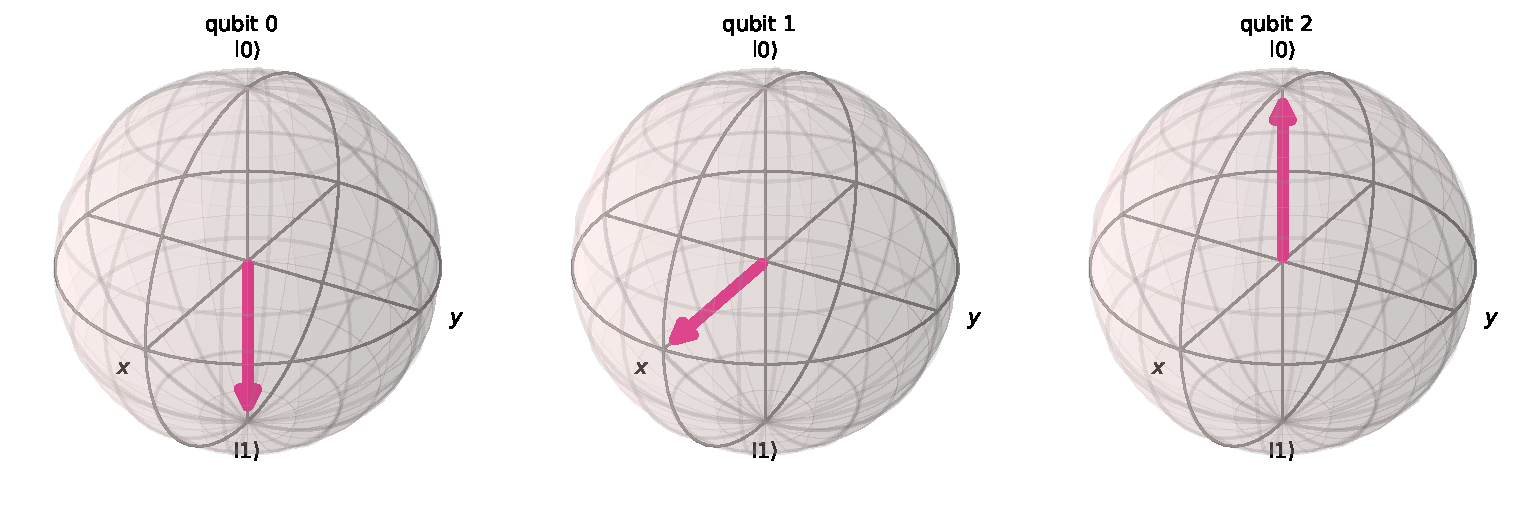
\includegraphics[keepaspectratio]{apostila_files/figure-pdf/cell-54-output-2.pdf}}

\pandocbounded{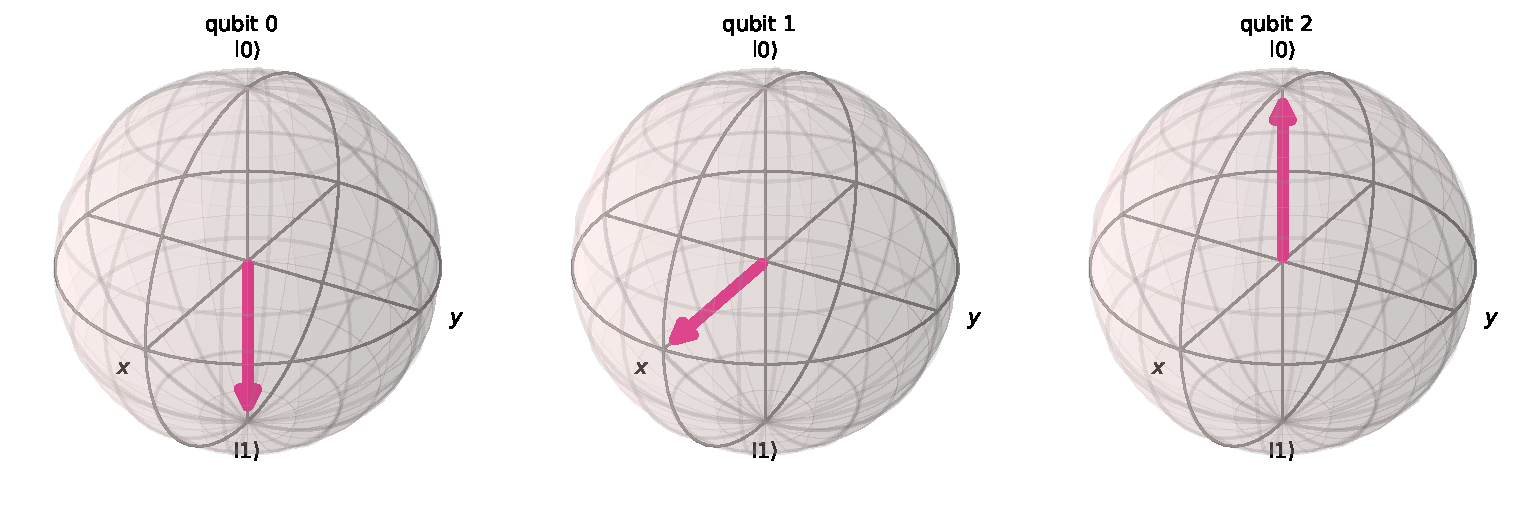
\includegraphics[keepaspectratio]{apostila_files/figure-pdf/cell-54-output-3.pdf}}

\begin{verbatim}
Statevector([0.        +0.j, 0.70710678+0.j, 0.        +0.j,
             0.70710678+0.j, 0.        +0.j, 0.        +0.j,
             0.        +0.j, 0.        +0.j],
            dims=(2, 2, 2))
\end{verbatim}

📊 \textbf{Interpretando a Esfera de Bloch:}

Observe o qubit q{[}1{]} na visualização acima - ele está agora
\textbf{no equador da esfera, no eixo +X} (apontando para a direita ➡️).

Isso mostra visualmente a \textbf{superposição} criada por Hadamard:

\begin{longtable}[]{@{}
  >{\raggedright\arraybackslash}p{(\linewidth - 4\tabcolsep) * \real{0.4615}}
  >{\raggedright\arraybackslash}p{(\linewidth - 4\tabcolsep) * \real{0.2051}}
  >{\raggedright\arraybackslash}p{(\linewidth - 4\tabcolsep) * \real{0.3333}}@{}}
\toprule\noalign{}
\begin{minipage}[b]{\linewidth}\raggedright
Posição na Bloch
\end{minipage} & \begin{minipage}[b]{\linewidth}\raggedright
Estado
\end{minipage} & \begin{minipage}[b]{\linewidth}\raggedright
Significado
\end{minipage} \\
\midrule\noalign{}
\endhead
\bottomrule\noalign{}
\endlastfoot
Polo Norte ⬆️ & \(\|0\rangle\) & Estado puro ``zero'' \\
Polo Sul ⬇️ & \(\|1\rangle\) & Estado puro ``um'' \\
Equador +X ➡️ & \(\frac{1}{\sqrt{2}}(\|0\rangle + \|1\rangle)\) &
\textbf{Superposição igual!} \\
Equador -X ⬅️ & \(\frac{1}{\sqrt{2}}(\|0\rangle - \|1\rangle)\) &
Superposição com fase \\
\end{longtable}

O qubit no equador indica que ele tem \textbf{50\% de chance} de ser
medido como 0 ou 1 - está literalmente em ambos os estados ao mesmo
tempo! ✨

⚠️ \textbf{Nota sobre visualizações:} A partir daqui, os qubits começam
a ficar emaranhados. A esfera de Bloch mostra apenas o \textbf{estado
reduzido} de cada qubit individual, mas \textbf{não captura as
correlações quânticas} (emaranhamento). Para ver a estrutura completa do
estado, vamos adicionar outras visualizações.

\textbf{Passo 3b - Aplicar CNOT entre q{[}1{]} e q{[}2{]}:}

A porta CNOT inverte o qubit alvo se o controle for \textbar1⟩:
\[CNOT|00\rangle = |00\rangle, \quad CNOT|10\rangle = |11\rangle\]

Aplicando CNOT(q{[}1{]}, q{[}2{]}):
\[|\psi_3\rangle = \frac{1}{\sqrt{2}}(|100\rangle + |111\rangle)\]

\textbf{🔗 Estado de Bell criado!} Os qubits 1 e 2 agora estão
\textbf{emaranhados} - medindo um, sabemos instantaneamente o outro!

\begin{Shaded}
\begin{Highlighting}[]
\NormalTok{circuit.cx(qreg\_q[}\DecValTok{1}\NormalTok{], qreg\_q[}\DecValTok{2}\NormalTok{])}

\NormalTok{state4 }\OperatorTok{=}\NormalTok{ Statevector.from\_instruction(circuit)}
\BuiltInTok{print}\NormalTok{(state4)}
\end{Highlighting}
\end{Shaded}

\begin{verbatim}
Statevector([0.        +0.j, 0.70710678+0.j, 0.        +0.j,
             0.        +0.j, 0.        +0.j, 0.        +0.j,
             0.        +0.j, 0.70710678+0.j],
            dims=(2, 2, 2))
\end{verbatim}

\begin{verbatim}
Statevector([0.        +0.j, 0.70710678+0.j, 0.        +0.j,
             0.        +0.j, 0.        +0.j, 0.        +0.j,
             0.        +0.j, 0.70710678+0.j],
            dims=(2, 2, 2))
\end{verbatim}

\begin{Shaded}
\begin{Highlighting}[]
\CommentTok{\# Visualização na Q{-}Sphere {-} melhor para ver emaranhamento!}
\BuiltInTok{print}\NormalTok{(}\StringTok{"}\CharTok{\textbackslash{}n}\StringTok{🌐 Q{-}Sphere (mostra amplitudes e fases do estado completo):"}\NormalTok{)}
\NormalTok{plot\_state\_qsphere(state4)}
\end{Highlighting}
\end{Shaded}

\begin{verbatim}

🌐 Q-Sphere (mostra amplitudes e fases do estado completo):
\end{verbatim}

\pandocbounded{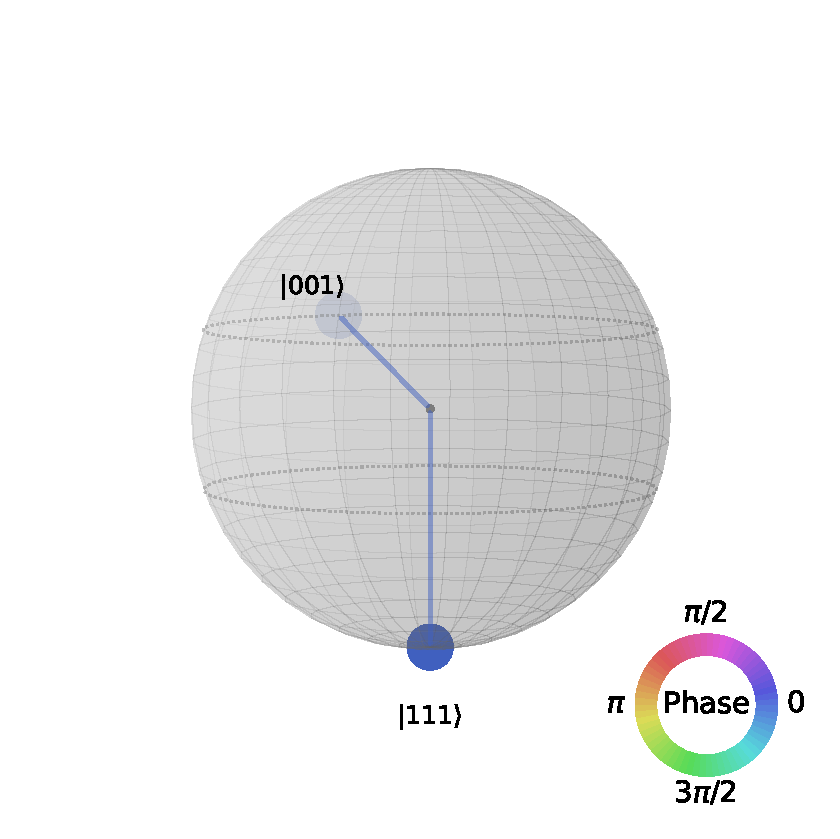
\includegraphics[keepaspectratio]{apostila_files/figure-pdf/cell-56-output-2.pdf}}

\pandocbounded{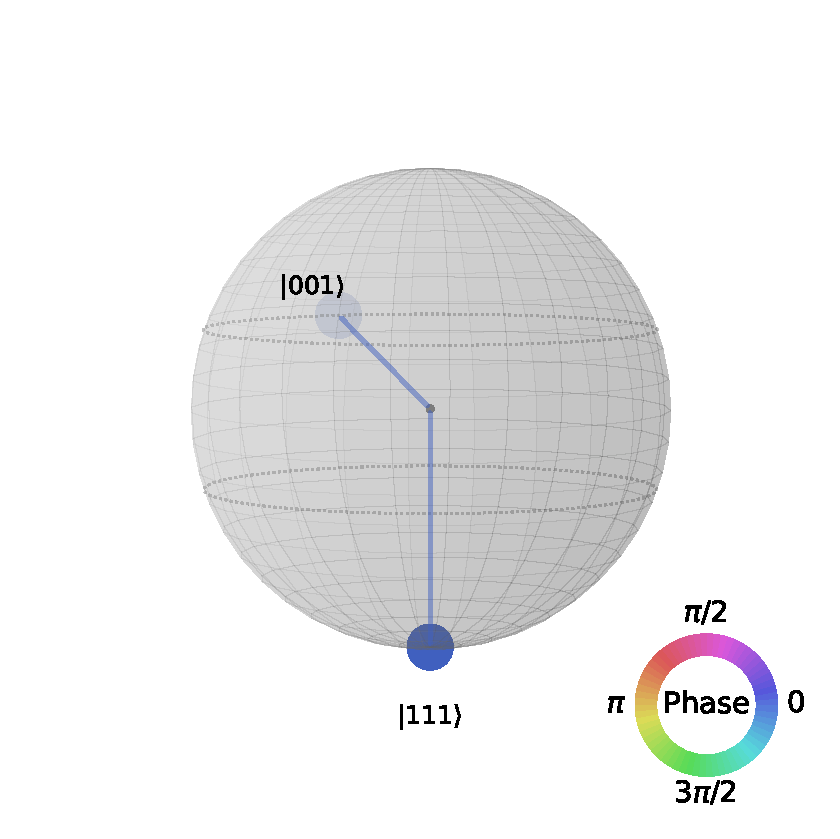
\includegraphics[keepaspectratio]{apostila_files/figure-pdf/cell-56-output-3.pdf}}

\begin{verbatim}

🌐 Q-Sphere (mostra amplitudes e fases do estado completo):
\end{verbatim}

\begin{Shaded}
\begin{Highlighting}[]
\CommentTok{\# 🌐 Visualização INTERATIVA da Q{-}Sphere}
\CommentTok{\# Importar a função do módulo quantum\_viz (localizado em ../src)}
\ImportTok{import}\NormalTok{ sys}
\ImportTok{from}\NormalTok{ pathlib }\ImportTok{import}\NormalTok{ Path}
\ControlFlowTok{for}\NormalTok{ p }\KeywordTok{in}\NormalTok{ [Path.cwd(), Path.cwd().parent, Path.cwd().parent.parent]:}
    \ControlFlowTok{if}\NormalTok{ (p }\OperatorTok{/} \StringTok{"src"}\NormalTok{).is\_dir() }\KeywordTok{and} \BuiltInTok{str}\NormalTok{(p }\OperatorTok{/} \StringTok{"src"}\NormalTok{) }\KeywordTok{not} \KeywordTok{in}\NormalTok{ sys.path:}
\NormalTok{        sys.path.insert(}\DecValTok{0}\NormalTok{, }\BuiltInTok{str}\NormalTok{(p }\OperatorTok{/} \StringTok{"src"}\NormalTok{))}
\ImportTok{from}\NormalTok{ quantum\_viz }\ImportTok{import}\NormalTok{ plot\_qsphere\_interactive}

\CommentTok{\# 🎨 Criar e exibir a visualização}
\BuiltInTok{print}\NormalTok{(}\StringTok{"}\CharTok{\textbackslash{}n}\StringTok{🌐 Q{-}Sphere INTERATIVA:"}\NormalTok{)}
\BuiltInTok{print}\NormalTok{(}\StringTok{"   → Magenta = Fase positiva (+)"}\NormalTok{)}
\BuiltInTok{print}\NormalTok{(}\StringTok{"   → Ciano = Fase negativa ({-})"}\NormalTok{)}
\BuiltInTok{print}\NormalTok{(}\StringTok{"   → Tamanho = Probabilidade}\CharTok{\textbackslash{}n}\StringTok{"}\NormalTok{)}

\CommentTok{\# A função plot\_qsphere\_interactive salva automaticamente e abre no navegador}
\NormalTok{fig }\OperatorTok{=}\NormalTok{ plot\_qsphere\_interactive(state4)}
\end{Highlighting}
\end{Shaded}

\begin{verbatim}

🌐 Q-Sphere INTERATIVA:
   → Magenta = Fase positiva (+)
   → Ciano = Fase negativa (-)
   → Tamanho = Probabilidade

✅ Visualização 3D salva em: /home/max/aula-quantum/content/qsphere_interativa.html
\end{verbatim}

\begin{verbatim}

🌐 Q-Sphere INTERATIVA:
   → Magenta = Fase positiva (+)
   → Ciano = Fase negativa (-)
   → Tamanho = Probabilidade

✅ Visualização 3D salva em: e:\temp\quantum\notebooks\qsphere_interativa.html
   Abrindo no navegador...

💡 Dica: Você pode arrastar, girar e dar zoom na esfera!
   O arquivo HTML pode ser aberto a qualquer momento.
\end{verbatim}

\subsubsection{🌐 O que é a Q-Sphere e o que ela está
mostrando?}\label{o-que-uxe9-a-q-sphere-e-o-que-ela-estuxe1-mostrando}

A \textbf{Q-Sphere} (Esfera Quântica) é uma visualização poderosa que
mostra o \textbf{estado completo de um sistema quântico} de múltiplos
qubits. Diferente da Esfera de Bloch, que mostra apenas qubits
individuais, a Q-Sphere revela todo o sistema de uma só vez.

\textbf{Como interpretar a Q-Sphere:}

\begin{enumerate}
\def\labelenumi{\arabic{enumi}.}
\tightlist
\item
  \textbf{Pontos na superfície da esfera:}

  \begin{itemize}
  \tightlist
  \item
    Cada ponto representa um \textbf{estado da base computacional}
  \item
    Para 3 qubits: 8 pontos possíveis (\textbar000⟩, \textbar001⟩,
    \textbar010⟩, \textbar011⟩, \textbar100⟩, \textbar101⟩,
    \textbar110⟩, \textbar111⟩)
  \item
    Os pontos são distribuídos na superfície da esfera seguindo uma
    convenção geométrica
  \end{itemize}
\item
  \textbf{Tamanho dos círculos:}

  \begin{itemize}
  \tightlist
  \item
    O \textbf{diâmetro} de cada círculo é proporcional à
    \textbf{amplitude} (probabilidade) daquele estado
  \item
    Círculo maior = maior probabilidade de medir aquele estado ao
    colapsar
  \item
    Sem círculo (ponto vazio) = amplitude zero (estado não contribui)
  \end{itemize}
\item
  \textbf{Cores dos círculos:}

  \begin{itemize}
  \tightlist
  \item
    \textbf{Rosa/Magenta}: Amplitude com fase \textbf{positiva} (+)
  \item
    \textbf{Verde/Ciano}: Amplitude com fase \textbf{negativa} (-)
  \item
    A cor mostra a \textbf{fase relativa} entre os componentes do estado
  \end{itemize}
\end{enumerate}

\textbf{O que estamos vendo neste momento:}

Após aplicar H em q{[}1{]} e CNOT entre q{[}1{]} e q{[}2{]}, criamos o
estado:

\[|\psi_3\rangle = \frac{1}{\sqrt{2}}(|100\rangle + |111\rangle)\]

Na Q-Sphere, você deverá ver:

\begin{itemize}
\tightlist
\item
  \textbf{Apenas 2 círculos visíveis} (dos 8 pontos possíveis):

  \begin{itemize}
  \tightlist
  \item
    Um no ponto \textbar100⟩
  \item
    Um no ponto \textbar111⟩
  \end{itemize}
\item
  \textbf{Ambos com o mesmo tamanho}: pois
  \(\frac{1}{\sqrt{2}} \approx 0.707\)

  \begin{itemize}
  \tightlist
  \item
    Probabilidade de cada:
    \(\left|\frac{1}{\sqrt{2}}\right|^2 = \frac{1}{2} = 50\%\)
  \end{itemize}
\item
  \textbf{Ambos da mesma cor (rosa)}: pois ambos têm fase positiva (+)

  \begin{itemize}
  \tightlist
  \item
    O termo \(+|100\rangle\) tem sinal positivo
  \item
    O termo \(+|111\rangle\) tem sinal positivo
  \end{itemize}
\end{itemize}

\textbf{Por que isso é emaranhamento?}

Observe que só aparecem os estados \textbar100⟩ e \textbar111⟩: - Se
medirmos q{[}1{]} e obtivermos 0 → q{[}2{]} também será 0 (estado
\textbar100⟩) - Se medirmos q{[}1{]} e obtivermos 1 → q{[}2{]} também
será 1 (estado \textbar111⟩)

Os qubits 1 e 2 estão \textbf{perfeitamente correlacionados} - essa é a
assinatura visual do \textbf{emaranhamento quântico}! 🔗✨

A Q-Sphere nos permite ver essa correlação de forma clara: apenas
configurações onde q{[}1{]} = q{[}2{]} aparecem (00 ou 11 nos últimos
dois qubits).

\subsection{Continuando o Cálculo
Matemático}\label{continuando-o-cuxe1lculo-matemuxe1tico}

\textbf{Passo 3c - Aplicar CNOT entre q{[}0{]} e q{[}1{]}:}

Agora q{[}0{]} é o controle e q{[}1{]} é o alvo:
\[|\psi_4\rangle = \frac{1}{\sqrt{2}}(|110\rangle + |101\rangle)\]

\textbf{✨ Emaranhamento triplo!} Agora os 3 qubits estão
interconectados quanticamente.

\begin{Shaded}
\begin{Highlighting}[]
\NormalTok{circuit.cx(qreg\_q[}\DecValTok{0}\NormalTok{], qreg\_q[}\DecValTok{1}\NormalTok{])}

\NormalTok{state5 }\OperatorTok{=}\NormalTok{ Statevector.from\_instruction(circuit)}
\BuiltInTok{print}\NormalTok{(state5)}

\CommentTok{\# Visualização "City" {-} mostra a matriz densidade}
\BuiltInTok{print}\NormalTok{(}\StringTok{"}\CharTok{\textbackslash{}n}\StringTok{🏙️ State City (visualização 3D da matriz densidade):"}\NormalTok{)}
\NormalTok{plot\_state\_city(state5)}
\end{Highlighting}
\end{Shaded}

\begin{verbatim}
Statevector([0.        +0.j, 0.        +0.j, 0.        +0.j,
             0.70710678+0.j, 0.        +0.j, 0.70710678+0.j,
             0.        +0.j, 0.        +0.j],
            dims=(2, 2, 2))

🏙️ State City (visualização 3D da matriz densidade):
\end{verbatim}

\pandocbounded{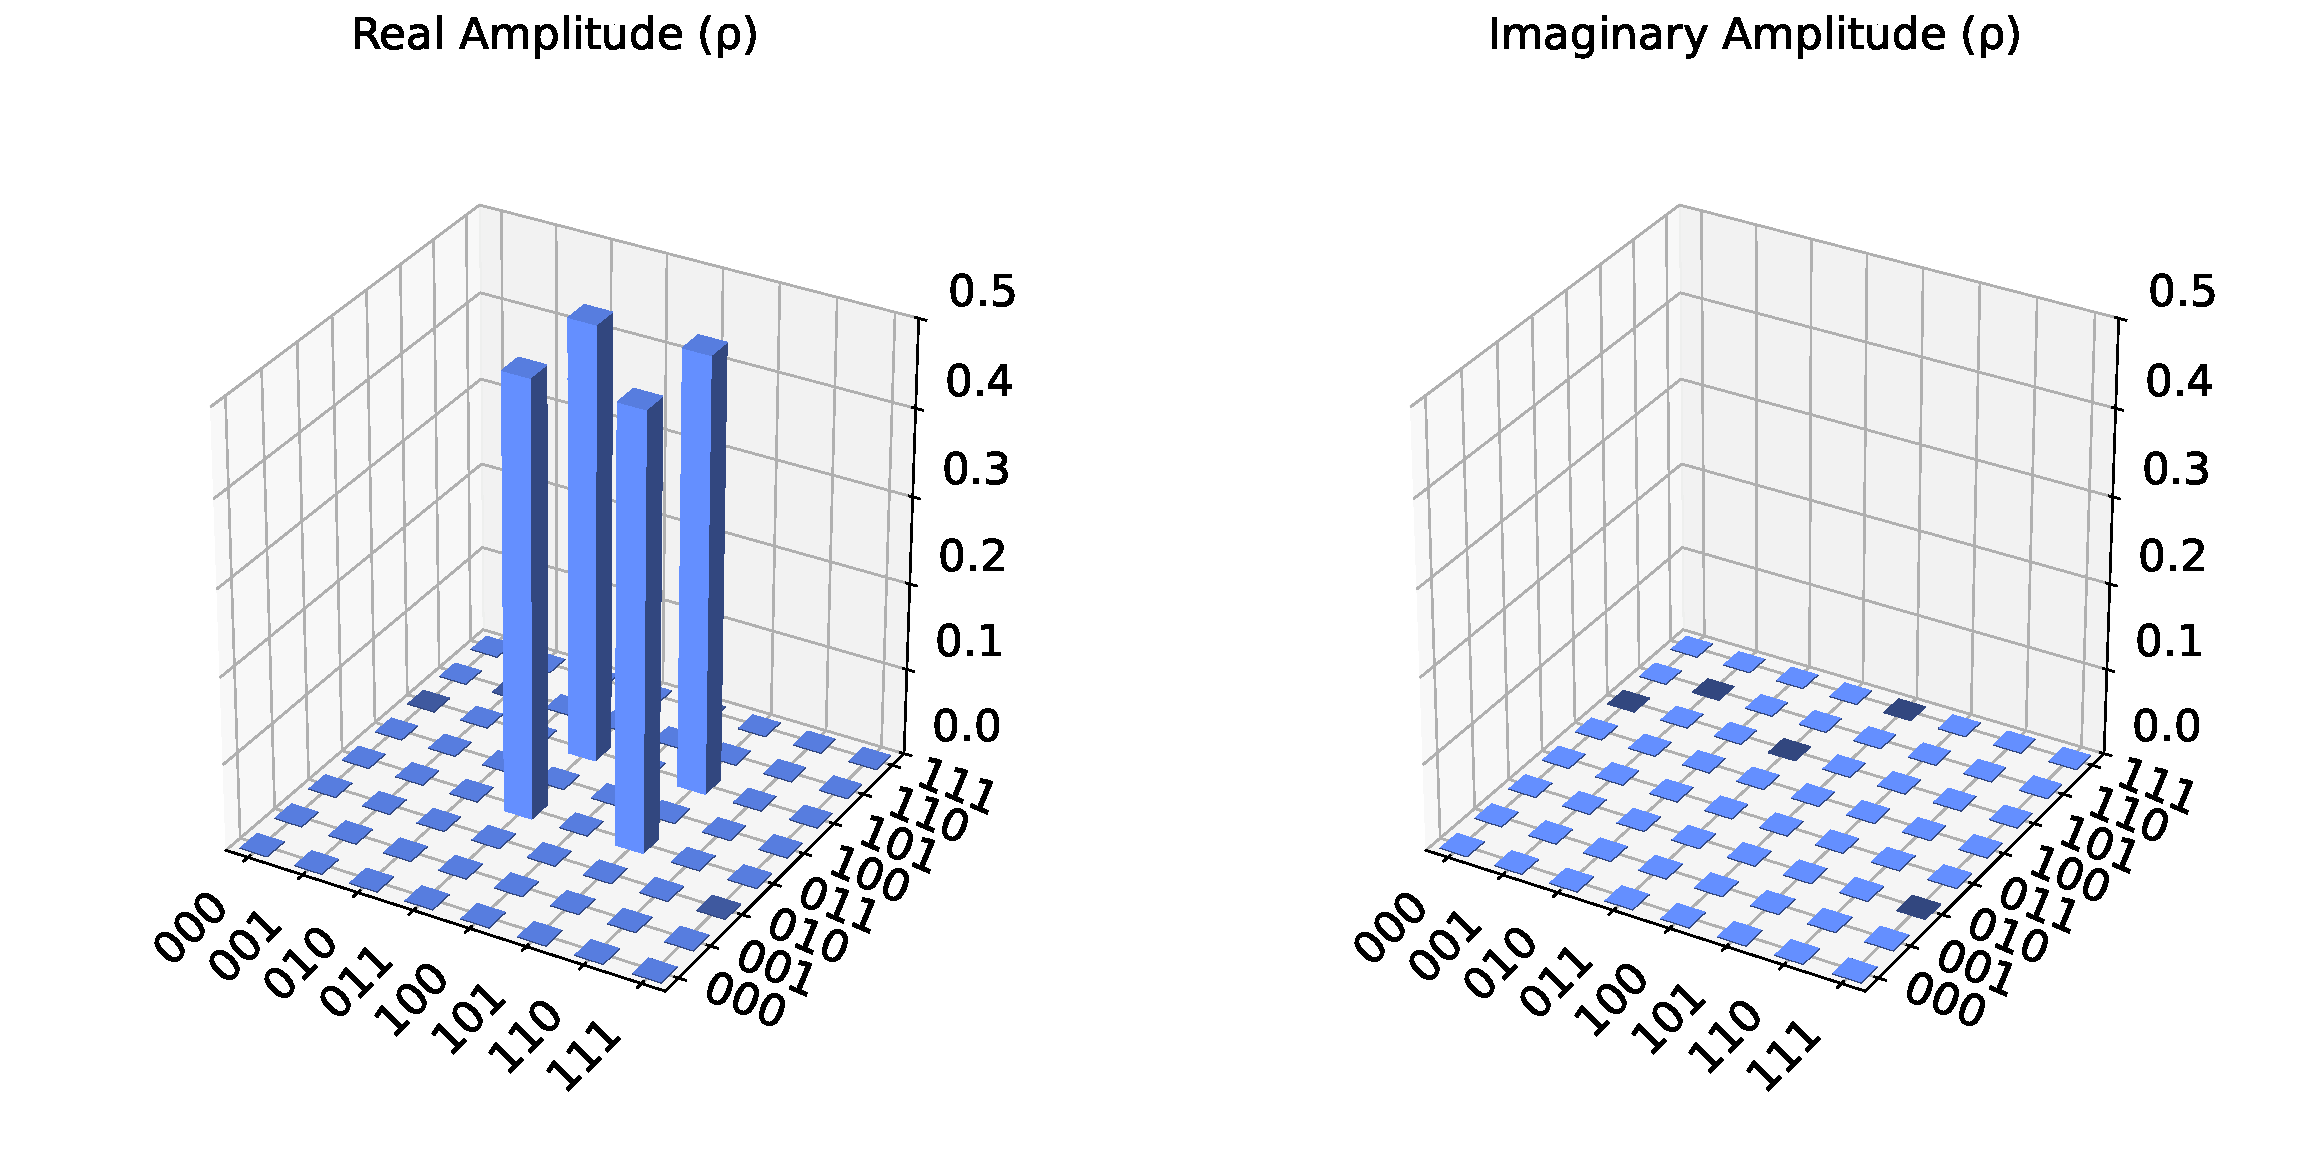
\includegraphics[keepaspectratio]{apostila_files/figure-pdf/cell-58-output-2.pdf}}

\pandocbounded{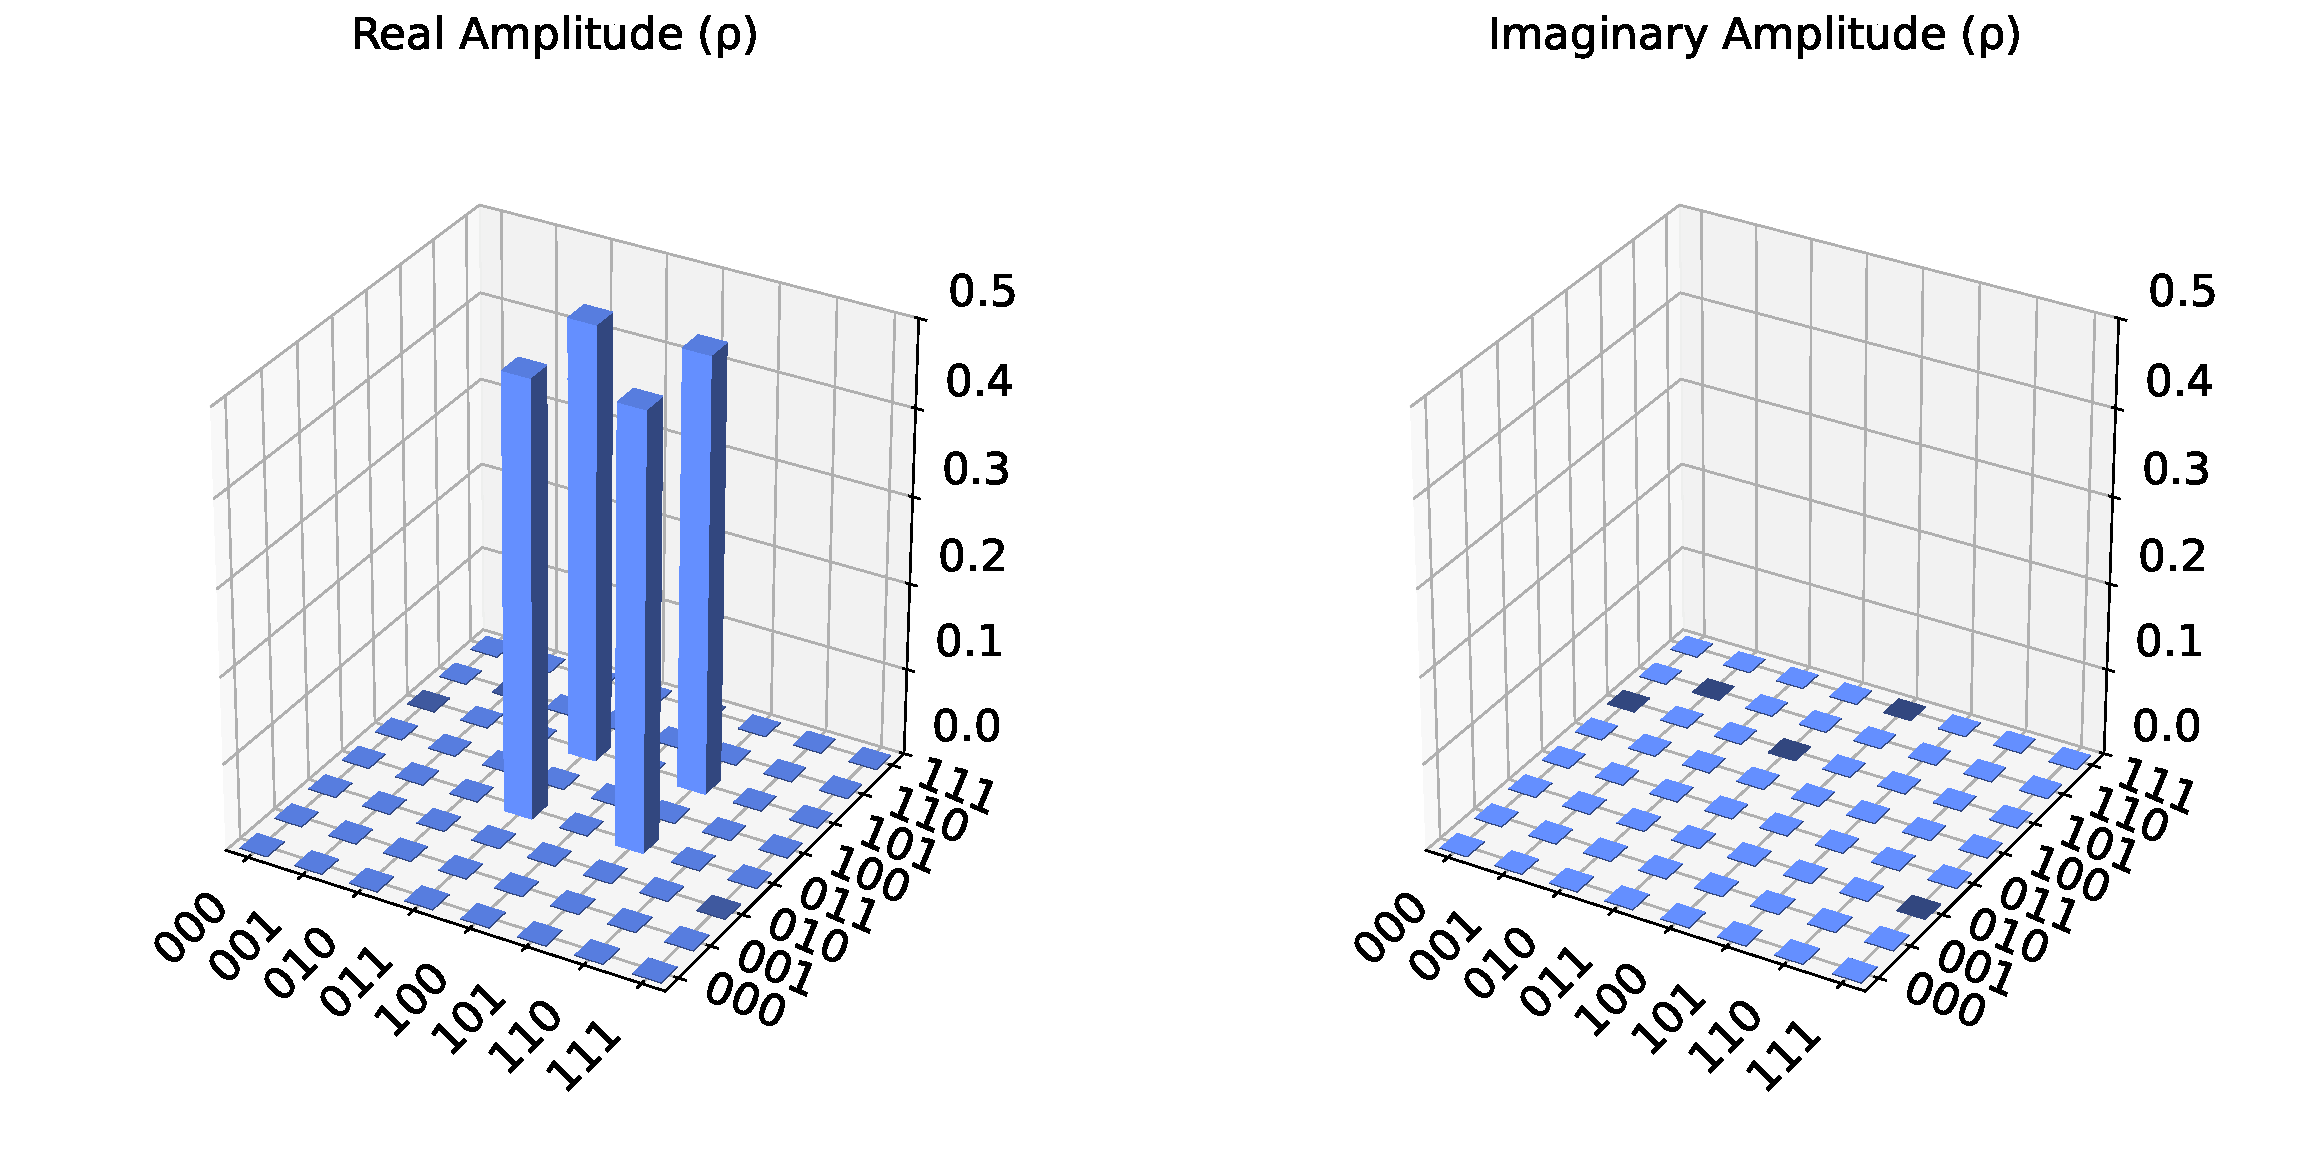
\includegraphics[keepaspectratio]{apostila_files/figure-pdf/cell-58-output-3.pdf}}

\begin{verbatim}
Statevector([0.        +0.j, 0.        +0.j, 0.        +0.j,
             0.70710678+0.j, 0.        +0.j, 0.70710678+0.j,
             0.        +0.j, 0.        +0.j],
            dims=(2, 2, 2))

🏙️ State City (visualização 3D da matriz densidade):
\end{verbatim}

\subsubsection{🏙️ O que é o State City e o que ele está
mostrando?}\label{o-que-uxe9-o-state-city-e-o-que-ele-estuxe1-mostrando}

O \textbf{State City} (Cidade dos Estados) é uma visualização 3D que
representa a \textbf{matriz densidade} de um estado quântico. É como um
``mapa de Manhattan'' onde cada ``prédio'' nos conta algo sobre o
sistema quântico.

\textbf{Conceitos fundamentais:}

\begin{enumerate}
\def\labelenumi{\arabic{enumi}.}
\tightlist
\item
  \textbf{Matriz Densidade (\(\rho\)):}

  \begin{itemize}
  \tightlist
  \item
    Para um estado puro \(|\psi\rangle\), a matriz densidade é
    \(\rho = |\psi\rangle\langle\psi|\)
  \item
    É uma matriz quadrada de dimensão \(2^n \times 2^n\) (para \(n\)
    qubits)
  \item
    Para 3 qubits: matriz \(8 \times 8\) (64 elementos)
  \end{itemize}
\item
  \textbf{Elementos da matriz:}

  \begin{itemize}
  \tightlist
  \item
    \textbf{Diagonal principal}: Probabilidades de cada estado (valores
    reais)
  \item
    \textbf{Fora da diagonal}: Coerências quânticas (podem ser
    complexos)
  \end{itemize}
\end{enumerate}

\textbf{Como interpretar o State City:}

\begin{enumerate}
\def\labelenumi{\arabic{enumi}.}
\tightlist
\item
  \textbf{Grade no ``chão'' (base XY):}

  \begin{itemize}
  \tightlist
  \item
    Eixo X: índice da linha da matriz densidade (estados base)
  \item
    Eixo Y: índice da coluna da matriz densidade (estados base)
  \item
    Para 3 qubits: 8×8 = 64 posições possíveis
  \end{itemize}
\item
  \textbf{Altura dos ``prédios'' (barras verticais):}

  \begin{itemize}
  \tightlist
  \item
    Representa a \textbf{magnitude} (valor absoluto) de cada elemento da
    matriz
  \item
    Prédios mais altos = valores maiores
  \item
    Sem prédio (vazio) = valor zero ou próximo de zero
  \end{itemize}
\item
  \textbf{Cores dos prédios:}

  \begin{itemize}
  \tightlist
  \item
    \textbf{Azul}: Valores reais positivos
  \item
    \textbf{Rosa/Vermelho}: Valores reais negativos (ou partes
    imaginárias)
  \item
    A intensidade da cor indica a magnitude
  \end{itemize}
\end{enumerate}

\textbf{O que estamos vendo neste momento:}

Após aplicar CNOT(q{[}0{]}, q{[}1{]}), temos o estado:

\[|\psi_4\rangle = \frac{1}{\sqrt{2}}(|110\rangle + |101\rangle)\]

Na visualização State City, você verá:

\begin{itemize}
\tightlist
\item
  \textbf{Diagonal principal} (linha de prédios de canto a canto):

  \begin{itemize}
  \tightlist
  \item
    Apenas 2 prédios destacados nas posições correspondentes a
    \textbar110⟩ e \textbar101⟩
  \item
    Ambos com altura \(\frac{1}{2}\) (probabilidade de 50\% cada)
  \item
    Outros elementos da diagonal são zero (outros estados não aparecem)
  \end{itemize}
\item
  \textbf{Elementos fora da diagonal} (coerências):

  \begin{itemize}
  \tightlist
  \item
    Representam a \textbf{interferência quântica} entre \textbar110⟩ e
    \textbar101⟩
  \item
    Esses prédios mostram que o sistema está em \textbf{superposição}
  \item
    Indicam correlações quânticas (emaranhamento) entre os 3 qubits
  \end{itemize}
\end{itemize}

\textbf{Por que isso mostra emaranhamento triplo?}

Os elementos fora da diagonal conectam estados diferentes (\textbar110⟩
↔ \textbar101⟩), mostrando que: - Os qubits não podem ser descritos
individualmente - Existe uma \textbf{correlação quântica genuína} entre
os 3 qubits - Medindo um qubit, afetamos instantaneamente o estado dos
outros

\textbf{State City vs outras visualizações:}

\begin{longtable}[]{@{}
  >{\raggedright\arraybackslash}p{(\linewidth - 4\tabcolsep) * \real{0.3415}}
  >{\raggedright\arraybackslash}p{(\linewidth - 4\tabcolsep) * \real{0.3415}}
  >{\raggedright\arraybackslash}p{(\linewidth - 4\tabcolsep) * \real{0.3171}}@{}}
\toprule\noalign{}
\begin{minipage}[b]{\linewidth}\raggedright
Visualização
\end{minipage} & \begin{minipage}[b]{\linewidth}\raggedright
O que mostra
\end{minipage} & \begin{minipage}[b]{\linewidth}\raggedright
Quando usar
\end{minipage} \\
\midrule\noalign{}
\endhead
\bottomrule\noalign{}
\endlastfoot
\textbf{Esfera de Bloch} & Estados individuais de cada qubit & 1 qubit,
transformações unitárias \\
\textbf{Q-Sphere} & Amplitudes e fases na base computacional & Ver
superposição e fase \\
\textbf{State City} & Estrutura completa da matriz densidade & Ver
coerências e emaranhamento \\
\end{longtable}

O State City é particularmente útil para visualizar \textbf{estados
emaranhados} porque as coerências (prédios fora da diagonal) revelam as
correlações quânticas que não existem em estados separáveis! 🏙️✨

\subsection{Continuando o Cálculo
Matemático}\label{continuando-o-cuxe1lculo-matemuxe1tico-1}

\textbf{Passo 3d - Aplicar Hadamard em q{[}0{]}:}

Expandindo \(H\) em cada componente:
\[H|1\rangle = \frac{1}{\sqrt{2}}(|0\rangle - |1\rangle)\]

Estado final antes da medição:
\[|\psi_5\rangle = \frac{1}{2}(|010\rangle - |110\rangle + |001\rangle - |101\rangle)\]

Podemos reescrever agrupando os estados de Alice (q{[}0{]}q{[}1{]}) e
Bob (q{[}2{]}):
\[|\psi_5\rangle = \frac{1}{2}[|00\rangle(|0\rangle - |1\rangle) + |01\rangle(|1\rangle - |0\rangle) + |10\rangle(|0\rangle + |1\rangle) + |11\rangle(|1\rangle + |0\rangle)]\]

\begin{Shaded}
\begin{Highlighting}[]
\NormalTok{circuit.h(qreg\_q[}\DecValTok{0}\NormalTok{])}
\NormalTok{circuit.barrier(qreg\_q[}\DecValTok{0}\NormalTok{], qreg\_q[}\DecValTok{1}\NormalTok{], qreg\_q[}\DecValTok{2}\NormalTok{])}
\NormalTok{circuit.draw(}\StringTok{\textquotesingle{}mpl\textquotesingle{}}\NormalTok{)}

\NormalTok{state6 }\OperatorTok{=}\NormalTok{ Statevector.from\_instruction(circuit)}
\BuiltInTok{print}\NormalTok{(state6)}

\CommentTok{\# Visualização combinada para o estado mais complexo}
\BuiltInTok{print}\NormalTok{(}\StringTok{"}\CharTok{\textbackslash{}n}\StringTok{🌐 Q{-}Sphere {-} Estado completo antes da medição:"}\NormalTok{)}
\NormalTok{plot\_state\_qsphere(state6)}
\end{Highlighting}
\end{Shaded}

\begin{verbatim}
Statevector([ 0. +0.j,  0. +0.j,  0.5+0.j, -0.5+0.j,  0.5+0.j, -0.5+0.j,
              0. +0.j,  0. +0.j],
            dims=(2, 2, 2))

🌐 Q-Sphere - Estado completo antes da medição:
\end{verbatim}

\pandocbounded{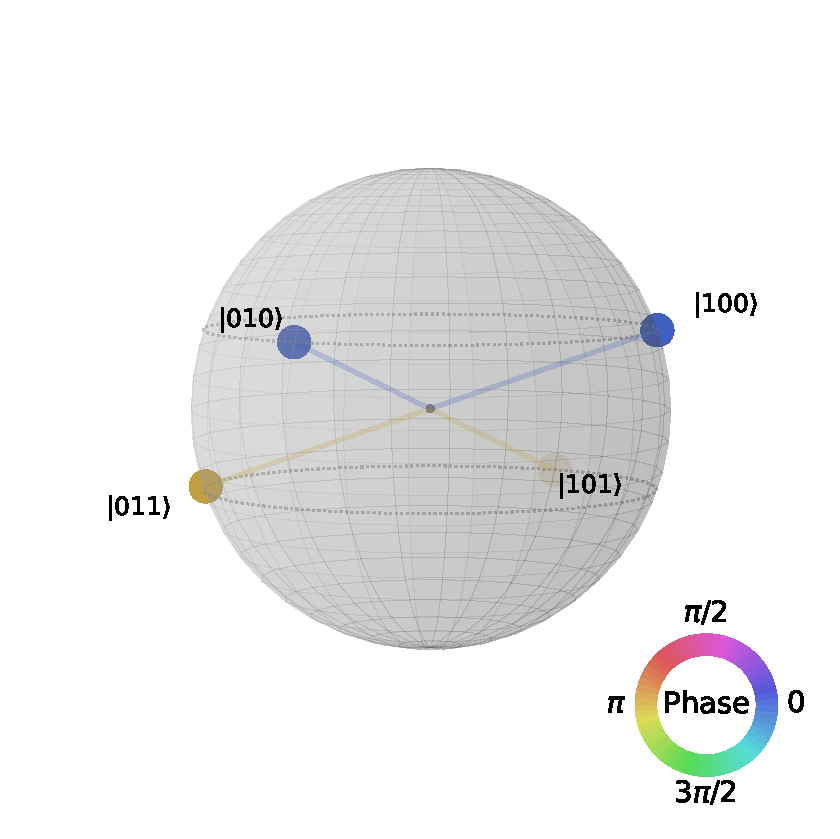
\includegraphics[keepaspectratio]{apostila_files/figure-pdf/cell-59-output-2.pdf}}

\pandocbounded{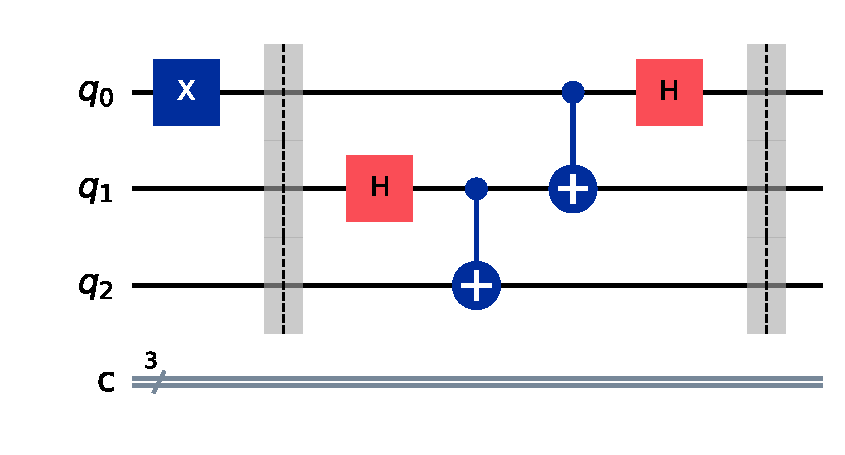
\includegraphics[keepaspectratio]{apostila_files/figure-pdf/cell-59-output-3.pdf}}

\pandocbounded{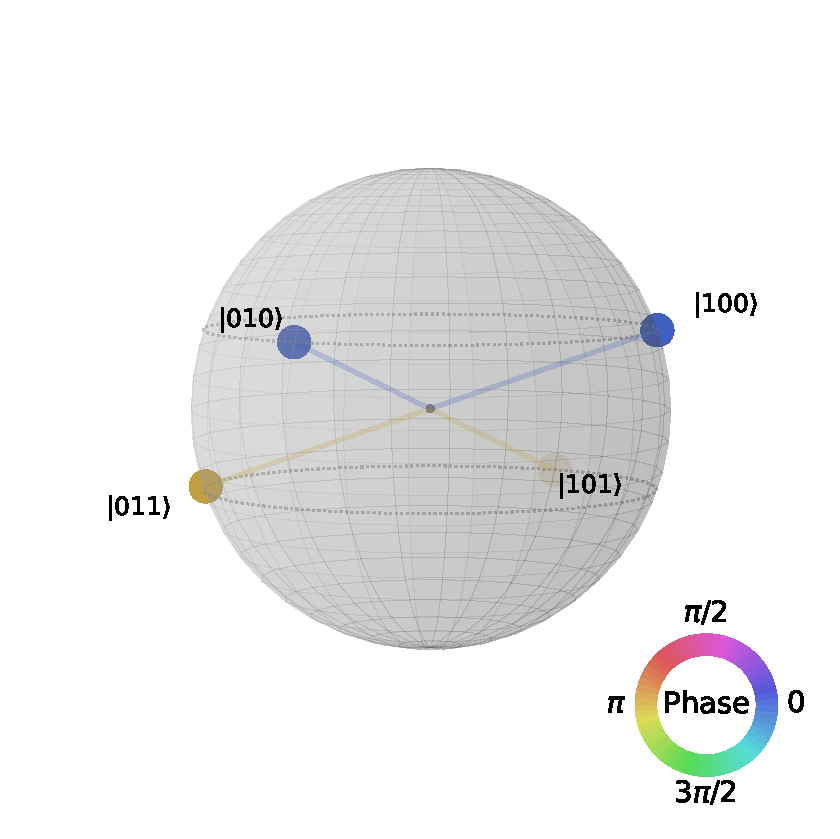
\includegraphics[keepaspectratio]{apostila_files/figure-pdf/cell-59-output-4.pdf}}

\begin{verbatim}
Statevector([ 0. +0.j,  0. +0.j,  0.5+0.j, -0.5+0.j,  0.5+0.j, -0.5+0.j,
              0. +0.j,  0. +0.j],
            dims=(2, 2, 2))

🌐 Q-Sphere - Estado completo antes da medição:
\end{verbatim}

\section{4️⃣ Passo 4: Alice ``Liga'' para
Bob}\label{passo-4-alice-liga-para-bob}

\textbf{Alice} agora mede seus dois qubits (0 e 1) e obtém resultados
clássicos.

📞 \textbf{A ligação telefônica:}

\begin{itemize}
\tightlist
\item
  Alice mede q{[}0{]} → resultado vai para c{[}0{]} (pode ser 0 ou 1)
\item
  Alice mede q{[}1{]} → resultado vai para c{[}1{]} (pode ser 0 ou 1)
\item
  Alice envia esses 2 bits clássicos para Bob (por telefone, internet,
  pombo-correio\ldots)
\end{itemize}

⚠️ \textbf{Importante:} Sem essa comunicação clássica, Bob não consegue
recuperar o estado!

🎯 \textbf{O que esses números dizem a Bob:} - Eles informam QUAL
correção Bob precisa fazer no qubit dele (q{[}2{]}) - São como
``instruções de montagem''

\subsection{📐 Análise Matemática da
Medição}\label{anuxe1lise-matemuxe1tica-da-mediuxe7uxe3o}

Do estado
\(|\psi_5\rangle = \frac{1}{2}(|010\rangle - |110\rangle + |001\rangle - |101\rangle)\),
quando Alice mede seus qubits, há 4 possíveis resultados:

\begin{longtable}[]{@{}
  >{\raggedright\arraybackslash}p{(\linewidth - 6\tabcolsep) * \real{0.2418}}
  >{\raggedright\arraybackslash}p{(\linewidth - 6\tabcolsep) * \real{0.1648}}
  >{\raggedright\arraybackslash}p{(\linewidth - 6\tabcolsep) * \real{0.3626}}
  >{\raggedright\arraybackslash}p{(\linewidth - 6\tabcolsep) * \real{0.2308}}@{}}
\toprule\noalign{}
\begin{minipage}[b]{\linewidth}\raggedright
Medição Alice (q₀q₁)
\end{minipage} & \begin{minipage}[b]{\linewidth}\raggedright
Probabilidade
\end{minipage} & \begin{minipage}[b]{\linewidth}\raggedright
Estado de Bob (q₂) após medição
\end{minipage} & \begin{minipage}[b]{\linewidth}\raggedright
Correção necessária
\end{minipage} \\
\midrule\noalign{}
\endhead
\bottomrule\noalign{}
\endlastfoot
\(\|00\rangle\) & 25\% & \(\|1\rangle\) & Nenhuma (já é
\(\|1\rangle\)!) \\
\(\|01\rangle\) & 25\% & \(\|0\rangle\) & Aplicar X para obter
\(\|1\rangle\) \\
\(\|10\rangle\) & 25\% & \(-\|1\rangle\) & Aplicar Z para corrigir fase
→ \(\|1\rangle\) \\
\(\|11\rangle\) & 25\% & \(-\|0\rangle\) & Aplicar X e Z para obter
\(\|1\rangle\) \\
\end{longtable}

\textbf{Como interpretar:} - Cada termo do estado corresponde a um
possível resultado de medição - A medição colapsa o estado para um dos 4
cenários com igual probabilidade - O estado de Bob está ``embaralhado''
- precisa das correções para recuperar \(|1\rangle\)

\begin{Shaded}
\begin{Highlighting}[]
\NormalTok{circuit.measure(qreg\_q[}\DecValTok{0}\NormalTok{], creg\_c[}\DecValTok{0}\NormalTok{])}
\NormalTok{circuit.measure(qreg\_q[}\DecValTok{1}\NormalTok{], creg\_c[}\DecValTok{1}\NormalTok{])}
\NormalTok{circuit.barrier(qreg\_q[}\DecValTok{0}\NormalTok{], qreg\_q[}\DecValTok{1}\NormalTok{], qreg\_q[}\DecValTok{2}\NormalTok{])}
\NormalTok{circuit.draw(}\StringTok{\textquotesingle{}mpl\textquotesingle{}}\NormalTok{)}
\end{Highlighting}
\end{Shaded}

\pandocbounded{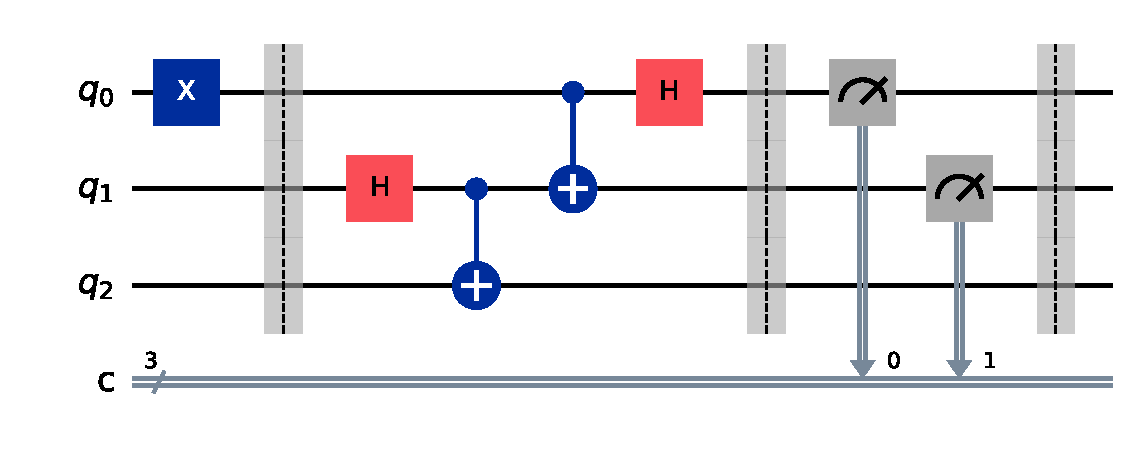
\includegraphics[keepaspectratio]{apostila_files/figure-pdf/cell-60-output-1.pdf}}

\pandocbounded{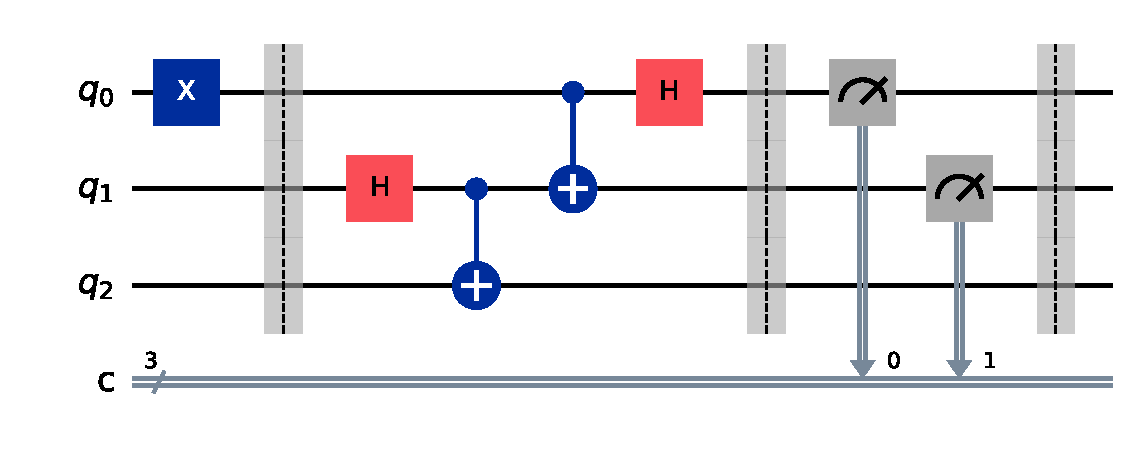
\includegraphics[keepaspectratio]{apostila_files/figure-pdf/cell-60-output-2.pdf}}

\section{5️⃣ Passo 5: Bob Recebe e ``Desempacota'' o
Estado!}\label{passo-5-bob-recebe-e-desempacota-o-estado}

\textbf{Bob} usa as instruções de Alice para corrigir seu qubit e obter
o estado original.

🔧 \textbf{As correções de Bob:}

\begin{enumerate}
\def\labelenumi{\arabic{enumi}.}
\tightlist
\item
  \textbf{CNOT(q{[}1{]}, q{[}2{]})} - Se c{[}1{]} = 1, aplica correção X

  \begin{itemize}
  \tightlist
  \item
    Pense: ``Se Alice disse `1', viro meu qubit''
  \end{itemize}
\item
  \textbf{CZ(q{[}0{]}, q{[}2{]})} - Se c{[}0{]} = 1, aplica correção Z

  \begin{itemize}
  \tightlist
  \item
    Pense: ``Se Alice disse `1', mudo a fase do meu qubit''
  \end{itemize}
\end{enumerate}

🎯 \textbf{Verificação:} Medimos q{[}2{]} → c{[}2{]} para confirmar que
recebemos \textbar1⟩

✨ \textbf{Resultado:} O qubit 2 de Bob agora está no estado \textbar1⟩
original!

\subsection{📐 Tabela de Correções Matemáticas -
COMPLETA}\label{tabela-de-correuxe7uxf5es-matemuxe1ticas---completa}

Bob aplica correções baseadas nos bits que Alice enviou. Vamos calcular
cada caso:

\begin{longtable}[]{@{}
  >{\raggedright\arraybackslash}p{(\linewidth - 8\tabcolsep) * \real{0.1852}}
  >{\raggedright\arraybackslash}p{(\linewidth - 8\tabcolsep) * \real{0.2222}}
  >{\raggedright\arraybackslash}p{(\linewidth - 8\tabcolsep) * \real{0.1852}}
  >{\raggedright\arraybackslash}p{(\linewidth - 8\tabcolsep) * \real{0.2346}}
  >{\raggedright\arraybackslash}p{(\linewidth - 8\tabcolsep) * \real{0.1728}}@{}}
\toprule\noalign{}
\begin{minipage}[b]{\linewidth}\raggedright
Medição Alice
\end{minipage} & \begin{minipage}[b]{\linewidth}\raggedright
Estado Bob antes
\end{minipage} & \begin{minipage}[b]{\linewidth}\raggedright
Operações Bob
\end{minipage} & \begin{minipage}[b]{\linewidth}\raggedright
Cálculo detalhado
\end{minipage} & \begin{minipage}[b]{\linewidth}\raggedright
Estado final
\end{minipage} \\
\midrule\noalign{}
\endhead
\bottomrule\noalign{}
\endlastfoot
\textbf{c{[}0{]}=0, c{[}1{]}=0} & \(-\|1\rangle\) & \(X^0 Z^0 = I\) &
\(I \cdot (-\|1\rangle) = -\|1\rangle\) & \(\|1\rangle\)* \\
\textbf{c{[}0{]}=0, c{[}1{]}=1} & \(\|0\rangle\) & \(X^1 Z^0 = X\) &
\(X\|0\rangle = \|1\rangle\) & \(\|1\rangle\) \\
\textbf{c{[}0{]}=1, c{[}1{]}=0} & \(-\|1\rangle\) & \(X^0 Z^1 = Z\) &
\(Z(-\|1\rangle) = -(-1)\|1\rangle = \|1\rangle\) & \(\|1\rangle\) \\
\textbf{c{[}0{]}=1, c{[}1{]}=1} & \(-\|0\rangle\) & \(X^1 Z^1 = XZ\) &
\(X(Z(-\|0\rangle)) = X(-\|0\rangle) = -\|1\rangle\) → \(\|1\rangle\)* &
\(\|1\rangle\) \\
\end{longtable}

\textbf{*Nota:} Fases globais (-1) não afetam medições - são fisicamente
indistinguíveis de \(|1\rangle\).

\subsection{🔄 Fluxo das Correções}\label{fluxo-das-correuxe7uxf5es}

\begin{verbatim}
Alice mede → 4 resultados possíveis → Bob corrige → Resultado: |1⟩

┌─────────────┬──────────────────┬────────────────┬──────────┐
│ Medição     │ Estado de Bob    │ Correção       │ Final    │
├─────────────┼──────────────────┼────────────────┼──────────┤
│ |00⟩ (25%)  │ -|1⟩             │ Nenhuma (I)    │ |1⟩      │
│ |01⟩ (25%)  │  |0⟩             │ X              │ |1⟩      │
│ |10⟩ (25%)  │ -|1⟩             │ Z              │ |1⟩      │
│ |11⟩ (25%)  │ -|0⟩             │ X, depois Z    │ |1⟩      │
└─────────────┴──────────────────┴────────────────┴──────────┘
\end{verbatim}

\subsection{🎓 Portas Utilizadas}\label{portas-utilizadas}

\textbf{Porta X (NOT quântico):}
\[X = \begin{pmatrix} 0 & 1 \\ 1 & 0 \end{pmatrix}, \quad X|0\rangle = |1\rangle, \quad X|1\rangle = |0\rangle\]

\textbf{Porta Z (inversão de fase):}
\[Z = \begin{pmatrix} 1 & 0 \\ 0 & -1 \end{pmatrix}, \quad Z|0\rangle = |0\rangle, \quad Z|1\rangle = -|1\rangle\]

\textbf{Porta CZ (Controlled-Z):}
\[CZ = \begin{pmatrix} 1 & 0 & 0 & 0 \\ 0 & 1 & 0 & 0 \\ 0 & 0 & 1 & 0 \\ 0 & 0 & 0 & -1 \end{pmatrix}\]

Aplica Z ao qubit alvo se o controle for \textbar1⟩.

🎉 \textbf{SUCESSO!} Em todos os casos, Bob recupera \(|1\rangle\) - o
estado foi teletransportado!

\begin{Shaded}
\begin{Highlighting}[]
\CommentTok{\# Aplicar as correções de Bob e fazer a medição final}
\NormalTok{circuit.cx(qreg\_q[}\DecValTok{1}\NormalTok{], qreg\_q[}\DecValTok{2}\NormalTok{])  }\CommentTok{\# Correção X condicional}
\NormalTok{circuit.cz(qreg\_q[}\DecValTok{0}\NormalTok{], qreg\_q[}\DecValTok{2}\NormalTok{])  }\CommentTok{\# Correção Z condicional}
\NormalTok{circuit.measure(qreg\_q[}\DecValTok{2}\NormalTok{], creg\_c[}\DecValTok{2}\NormalTok{])  }\CommentTok{\# Medir o qubit de Bob}
\NormalTok{circuit.draw(}\StringTok{\textquotesingle{}mpl\textquotesingle{}}\NormalTok{)}
\end{Highlighting}
\end{Shaded}

\pandocbounded{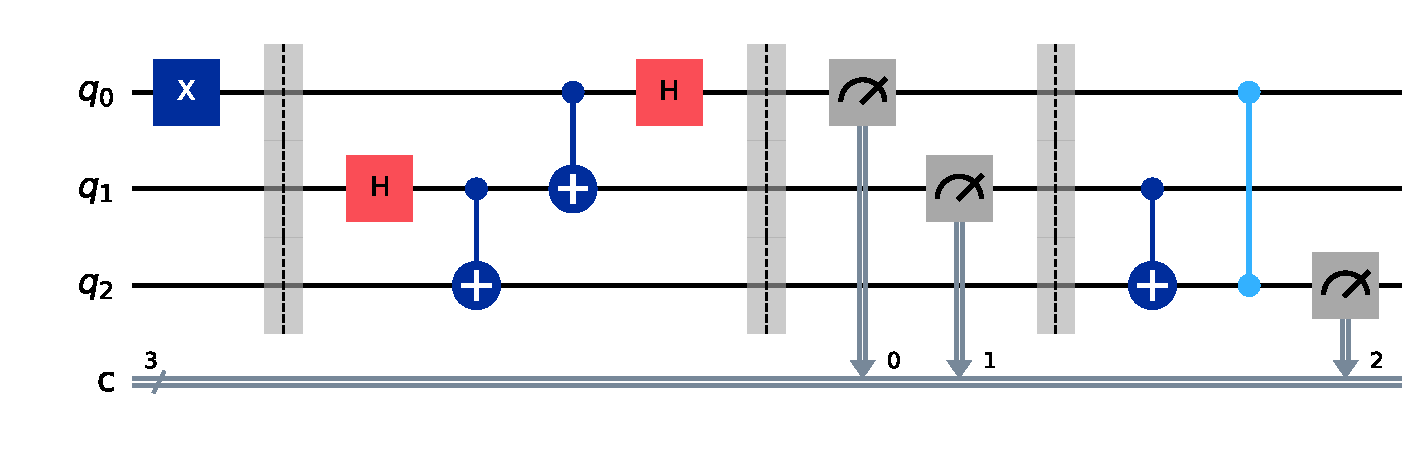
\includegraphics[keepaspectratio]{apostila_files/figure-pdf/cell-61-output-1.pdf}}

\pandocbounded{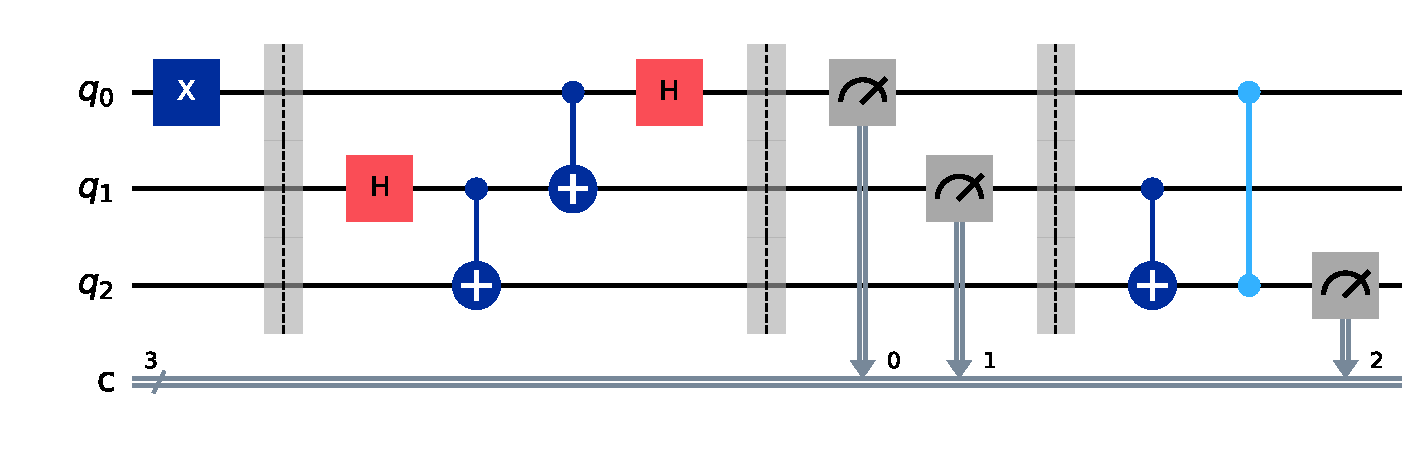
\includegraphics[keepaspectratio]{apostila_files/figure-pdf/cell-61-output-2.pdf}}

\subsection{🔬 Simulação: Verificando Cada
Cenário}\label{simulauxe7uxe3o-verificando-cada-cenuxe1rio}

Vamos simular cada um dos 4 possíveis cenários para confirmar
matematicamente que Bob sempre recebe \textbar1⟩:

\begin{Shaded}
\begin{Highlighting}[]
\ImportTok{import}\NormalTok{ numpy }\ImportTok{as}\NormalTok{ np}
\ImportTok{from}\NormalTok{ qiskit.quantum\_info }\ImportTok{import}\NormalTok{ Statevector, Operator}

\CommentTok{\# Estados de Bob após medição de Alice (da tabela do Passo 4)}
\NormalTok{cenarios }\OperatorTok{=}\NormalTok{ [}
\NormalTok{    (}\StringTok{"00"}\NormalTok{, np.array([}\DecValTok{0}\NormalTok{, }\OperatorTok{{-}}\DecValTok{1}\NormalTok{])),      }\CommentTok{\# {-}|1⟩}
\NormalTok{    (}\StringTok{"01"}\NormalTok{, np.array([}\DecValTok{1}\NormalTok{, }\DecValTok{0}\NormalTok{])),       }\CommentTok{\# |0⟩}
\NormalTok{    (}\StringTok{"10"}\NormalTok{, np.array([}\DecValTok{0}\NormalTok{, }\OperatorTok{{-}}\DecValTok{1}\NormalTok{])),      }\CommentTok{\# {-}|1⟩}
\NormalTok{    (}\StringTok{"11"}\NormalTok{, np.array([}\OperatorTok{{-}}\DecValTok{1}\NormalTok{, }\DecValTok{0}\NormalTok{]))       }\CommentTok{\# {-}|0⟩}
\NormalTok{]}

\BuiltInTok{print}\NormalTok{(}\StringTok{"🔬 Simulando os 4 cenários de teletransporte:}\CharTok{\textbackslash{}n}\StringTok{"}\NormalTok{)}
\BuiltInTok{print}\NormalTok{(}\StringTok{"="}\OperatorTok{*}\DecValTok{70}\NormalTok{)}

\CommentTok{\# Definir as portas}
\NormalTok{X }\OperatorTok{=}\NormalTok{ Operator([[}\DecValTok{0}\NormalTok{, }\DecValTok{1}\NormalTok{], [}\DecValTok{1}\NormalTok{, }\DecValTok{0}\NormalTok{]])}
\NormalTok{Z }\OperatorTok{=}\NormalTok{ Operator([[}\DecValTok{1}\NormalTok{, }\DecValTok{0}\NormalTok{], [}\DecValTok{0}\NormalTok{, }\OperatorTok{{-}}\DecValTok{1}\NormalTok{]])}

\ControlFlowTok{for}\NormalTok{ medicao, estado\_bob }\KeywordTok{in}\NormalTok{ cenarios:}
\NormalTok{    c0, c1 }\OperatorTok{=} \BuiltInTok{int}\NormalTok{(medicao[}\DecValTok{0}\NormalTok{]), }\BuiltInTok{int}\NormalTok{(medicao[}\DecValTok{1}\NormalTok{])}
    
    \CommentTok{\# Estado inicial de Bob neste cenário}
\NormalTok{    bob }\OperatorTok{=}\NormalTok{ Statevector(estado\_bob)}
    \BuiltInTok{print}\NormalTok{(}\SpecialStringTok{f"}\CharTok{\textbackslash{}n}\SpecialStringTok{📊 Cenário: Alice mediu |}\SpecialCharTok{\{}\NormalTok{medicao}\SpecialCharTok{\}}\SpecialStringTok{⟩"}\NormalTok{)}
    \BuiltInTok{print}\NormalTok{(}\SpecialStringTok{f"   Estado de Bob ANTES das correções: }\SpecialCharTok{\{}\NormalTok{bob}\SpecialCharTok{.}\NormalTok{data}\SpecialCharTok{\}}\SpecialStringTok{"}\NormalTok{)}
    
    \CommentTok{\# Aplicar correções de Bob (ordem: X depois Z)}
    \CommentTok{\# CNOT(c[1], Bob) = X se c[1]=1}
    \ControlFlowTok{if}\NormalTok{ c1 }\OperatorTok{==} \DecValTok{1}\NormalTok{:}
\NormalTok{        bob }\OperatorTok{=}\NormalTok{ bob.evolve(X)}
        \BuiltInTok{print}\NormalTok{(}\SpecialStringTok{f"   → Aplicou X (porque c[1]=1): }\SpecialCharTok{\{}\NormalTok{bob}\SpecialCharTok{.}\NormalTok{data}\SpecialCharTok{\}}\SpecialStringTok{"}\NormalTok{)}
    
    \CommentTok{\# CZ(c[0], Bob) = Z se c[0]=1  }
    \ControlFlowTok{if}\NormalTok{ c0 }\OperatorTok{==} \DecValTok{1}\NormalTok{:}
\NormalTok{        bob }\OperatorTok{=}\NormalTok{ bob.evolve(Z)}
        \BuiltInTok{print}\NormalTok{(}\SpecialStringTok{f"   → Aplicou Z (porque c[0]=1): }\SpecialCharTok{\{}\NormalTok{bob}\SpecialCharTok{.}\NormalTok{data}\SpecialCharTok{\}}\SpecialStringTok{"}\NormalTok{)}
    
    \CommentTok{\# Resultado final}
    \BuiltInTok{print}\NormalTok{(}\SpecialStringTok{f"   ✅ Estado FINAL de Bob: }\SpecialCharTok{\{}\NormalTok{bob}\SpecialCharTok{.}\NormalTok{data}\SpecialCharTok{\}}\SpecialStringTok{"}\NormalTok{)}
    
    \CommentTok{\# Verificar se é |1⟩ (ignorando fase global)}
\NormalTok{    esperado }\OperatorTok{=}\NormalTok{ np.array([}\DecValTok{0}\NormalTok{, }\DecValTok{1}\NormalTok{])}
    \ControlFlowTok{if}\NormalTok{ np.allclose(np.}\BuiltInTok{abs}\NormalTok{(bob.data), np.}\BuiltInTok{abs}\NormalTok{(esperado)):}
        \BuiltInTok{print}\NormalTok{(}\SpecialStringTok{f"   🎉 SUCESSO! Bob recebeu |1⟩"}\NormalTok{)}
    \ControlFlowTok{else}\NormalTok{:}
        \BuiltInTok{print}\NormalTok{(}\SpecialStringTok{f"   ❌ ERRO! Estado inesperado"}\NormalTok{)}

\BuiltInTok{print}\NormalTok{(}\StringTok{"}\CharTok{\textbackslash{}n}\StringTok{"} \OperatorTok{+} \StringTok{"="}\OperatorTok{*}\DecValTok{70}\NormalTok{)}
\BuiltInTok{print}\NormalTok{(}\StringTok{"✨ Conclusão: Em TODOS os 4 cenários, Bob recupera |1⟩!"}\NormalTok{)}
\BuiltInTok{print}\NormalTok{(}\StringTok{"   O teletransporte quântico funcionou perfeitamente! 🚀"}\NormalTok{)}
\end{Highlighting}
\end{Shaded}

\begin{verbatim}
🔬 Simulando os 4 cenários de teletransporte:

======================================================================

📊 Cenário: Alice mediu |00⟩
   Estado de Bob ANTES das correções: [ 0.+0.j -1.+0.j]
   ✅ Estado FINAL de Bob: [ 0.+0.j -1.+0.j]
   🎉 SUCESSO! Bob recebeu |1⟩

📊 Cenário: Alice mediu |01⟩
   Estado de Bob ANTES das correções: [1.+0.j 0.+0.j]
   → Aplicou X (porque c[1]=1): [0.+0.j 1.+0.j]
   ✅ Estado FINAL de Bob: [0.+0.j 1.+0.j]
   🎉 SUCESSO! Bob recebeu |1⟩

📊 Cenário: Alice mediu |10⟩
   Estado de Bob ANTES das correções: [ 0.+0.j -1.+0.j]
   → Aplicou Z (porque c[0]=1): [0.+0.j 1.+0.j]
   ✅ Estado FINAL de Bob: [0.+0.j 1.+0.j]
   🎉 SUCESSO! Bob recebeu |1⟩

📊 Cenário: Alice mediu |11⟩
   Estado de Bob ANTES das correções: [-1.+0.j  0.+0.j]
   → Aplicou X (porque c[1]=1): [ 0.+0.j -1.+0.j]
   → Aplicou Z (porque c[0]=1): [0.+0.j 1.+0.j]
   ✅ Estado FINAL de Bob: [0.+0.j 1.+0.j]
   🎉 SUCESSO! Bob recebeu |1⟩

======================================================================
✨ Conclusão: Em TODOS os 4 cenários, Bob recupera |1⟩!
   O teletransporte quântico funcionou perfeitamente! 🚀
\end{verbatim}

\begin{verbatim}
🔬 Simulando os 4 cenários de teletransporte:

======================================================================

📊 Cenário: Alice mediu |00⟩
   Estado de Bob ANTES das correções: [ 0.+0.j -1.+0.j]
   ✅ Estado FINAL de Bob: [ 0.+0.j -1.+0.j]
   🎉 SUCESSO! Bob recebeu |1⟩

📊 Cenário: Alice mediu |01⟩
   Estado de Bob ANTES das correções: [1.+0.j 0.+0.j]
   → Aplicou X (porque c[1]=1): [0.+0.j 1.+0.j]
   ✅ Estado FINAL de Bob: [0.+0.j 1.+0.j]
   🎉 SUCESSO! Bob recebeu |1⟩

📊 Cenário: Alice mediu |10⟩
   Estado de Bob ANTES das correções: [ 0.+0.j -1.+0.j]
   → Aplicou Z (porque c[0]=1): [0.+0.j 1.+0.j]
   ✅ Estado FINAL de Bob: [0.+0.j 1.+0.j]
   🎉 SUCESSO! Bob recebeu |1⟩

📊 Cenário: Alice mediu |11⟩
   Estado de Bob ANTES das correções: [-1.+0.j  0.+0.j]
   → Aplicou X (porque c[1]=1): [ 0.+0.j -1.+0.j]
   → Aplicou Z (porque c[0]=1): [0.+0.j 1.+0.j]
   ✅ Estado FINAL de Bob: [0.+0.j 1.+0.j]
   🎉 SUCESSO! Bob recebeu |1⟩

======================================================================
✨ Conclusão: Em TODOS os 4 cenários, Bob recupera |1⟩!
   O teletransporte quântico funcionou perfeitamente! 🚀
\end{verbatim}

\chapter{🔬 PARTE 2: Vamos Olhar ``Por Dentro'' do
Teletransporte!}\label{parte-2-vamos-olhar-por-dentro-do-teletransporte}

Agora que construímos o circuito completo, vamos usar o simulador para
ver o que está acontecendo em cada etapa.

\section{Por que isso é útil?}\label{por-que-isso-uxe9-uxfatil}

\begin{itemize}
\tightlist
\item
  Ver o estado quântico do sistema em diferentes momentos
\item
  Visualizar na esfera de Bloch (representação geométrica)
\item
  Confirmar que o teletransporte realmente funcionou!
\end{itemize}

💡 \textbf{Nota:} Na computação quântica real, não podemos ``espiar'' os
estados assim - a medição os destrói. Mas no simulador, podemos!

\section{⚠️ Por que Reconstruir os
Circuitos?}\label{por-que-reconstruir-os-circuitos}

Você deve estar se perguntando: \textbf{``Já temos o circuito
\texttt{circuit} completo, por que criar novos circuitos?''}

A resposta está em uma limitação fundamental da mecânica quântica:

\subsection{🚫 O Problema das
Medições}\label{o-problema-das-mediuxe7uxf5es}

O circuito \texttt{circuit} que construímos contém \textbf{operações de
medição} (\texttt{measure}). Quando medimos um qubit:

\begin{enumerate}
\def\labelenumi{\arabic{enumi}.}
\tightlist
\item
  \textbf{O estado quântico colapsa} → a superposição é destruída
\item
  \textbf{Obtemos apenas bits clássicos} (0 ou 1)
\item
  \textbf{Não podemos mais extrair o vetor de estado completo}
\end{enumerate}

\subsection{💻 Limitação do
Simulador}\label{limitauxe7uxe3o-do-simulador}

Se tentarmos fazer:

\begin{Shaded}
\begin{Highlighting}[]
\NormalTok{state }\OperatorTok{=}\NormalTok{ Statevector.from\_instruction(circuit)  }\CommentTok{\# ❌ ERRO!}
\end{Highlighting}
\end{Shaded}

O Qiskit retorna um \textbf{erro} porque \texttt{circuit} contém
medições, e após medir não existe mais um ``estado quântico'' para
visualizar.

\subsection{✅ A Solução: Circuitos Sem
Medições}\label{a-soluuxe7uxe3o-circuitos-sem-mediuxe7uxf5es}

Para \textbf{``espiar''} os estados intermediários, precisamos: -
Reconstruir o circuito \textbf{passo a passo} - \textbf{SEM} incluir as
medições - Usar apenas portas quânticas (X, H, CNOT, etc.)

Assim podemos usar \texttt{Statevector.from\_instruction()} e
\texttt{plot\_bloch\_multivector()} para ver o que está acontecendo
``por dentro''!

\subsection{🎓 Na Realidade vs.~No
Simulador}\label{na-realidade-vs.-no-simulador}

\begin{longtable}[]{@{}
  >{\raggedright\arraybackslash}p{(\linewidth - 2\tabcolsep) * \real{0.5200}}
  >{\raggedright\arraybackslash}p{(\linewidth - 2\tabcolsep) * \real{0.4800}}@{}}
\toprule\noalign{}
\begin{minipage}[b]{\linewidth}\raggedright
Computador Quântico Real
\end{minipage} & \begin{minipage}[b]{\linewidth}\raggedright
Simulador (nosso caso)
\end{minipage} \\
\midrule\noalign{}
\endhead
\bottomrule\noalign{}
\endlastfoot
❌ Não pode ``espiar'' estados & ✅ Pode reconstruir sem medições \\
❌ Medição é irreversível & ✅ Pode visualizar estados intermediários \\
✅ Apenas resultados finais & ✅ Vê todo o processo (didático) \\
\end{longtable}

A Parte 2 é um \textbf{privilégio educacional} do simulador! 🎯

\subsection{Construindo o Circuito Passo a
Passo}\label{construindo-o-circuito-passo-a-passo}

Vamos construir o circuito do teletransporte passo a passo, visualizando
o estado quântico após cada operação:

\begin{Shaded}
\begin{Highlighting}[]
\ImportTok{from}\NormalTok{ qiskit\_aer }\ImportTok{import}\NormalTok{ Aer}
\ImportTok{from}\NormalTok{ qiskit.quantum\_info }\ImportTok{import}\NormalTok{ Statevector}
\ImportTok{from}\NormalTok{ qiskit.visualization }\ImportTok{import}\NormalTok{ plot\_bloch\_multivector}

\CommentTok{\# Criar circuito (começando vazio)}
\NormalTok{final\_circuit }\OperatorTok{=}\NormalTok{ QuantumCircuit(}\DecValTok{3}\NormalTok{)}
\end{Highlighting}
\end{Shaded}

\subsubsection{🔹 Etapa 0: Estado Inicial (todos qubits em
\textbar0⟩)}\label{etapa-0-estado-inicial-todos-qubits-em-0}

\begin{Shaded}
\begin{Highlighting}[]
\CommentTok{\# Visualizar estado inicial (circuito vazio)}
\NormalTok{state\_0 }\OperatorTok{=}\NormalTok{ Statevector.from\_instruction(final\_circuit)}
\BuiltInTok{print}\NormalTok{(}\StringTok{"Estado: |000⟩ (todos qubits em |0⟩)"}\NormalTok{)}
\BuiltInTok{print}\NormalTok{(state\_0)}
\NormalTok{final\_circuit.draw(}\StringTok{\textquotesingle{}mpl\textquotesingle{}}\NormalTok{)}
\end{Highlighting}
\end{Shaded}

\begin{verbatim}
Estado: |000⟩ (todos qubits em |0⟩)
Statevector([1.+0.j, 0.+0.j, 0.+0.j, 0.+0.j, 0.+0.j, 0.+0.j, 0.+0.j,
             0.+0.j],
            dims=(2, 2, 2))
\end{verbatim}

\pandocbounded{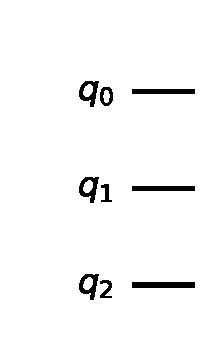
\includegraphics[keepaspectratio]{apostila_files/figure-pdf/cell-64-output-2.pdf}}

\pandocbounded{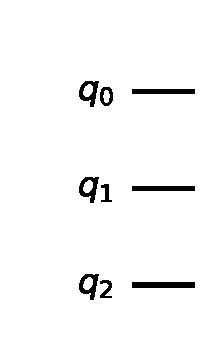
\includegraphics[keepaspectratio]{apostila_files/figure-pdf/cell-64-output-3.pdf}}

\begin{verbatim}
Estado: |000⟩ (todos qubits em |0⟩)
Statevector([1.+0.j, 0.+0.j, 0.+0.j, 0.+0.j, 0.+0.j, 0.+0.j, 0.+0.j,
             0.+0.j],
            dims=(2, 2, 2))
\end{verbatim}

\begin{Shaded}
\begin{Highlighting}[]
\NormalTok{plot\_bloch\_multivector(state\_0)}
\end{Highlighting}
\end{Shaded}

\pandocbounded{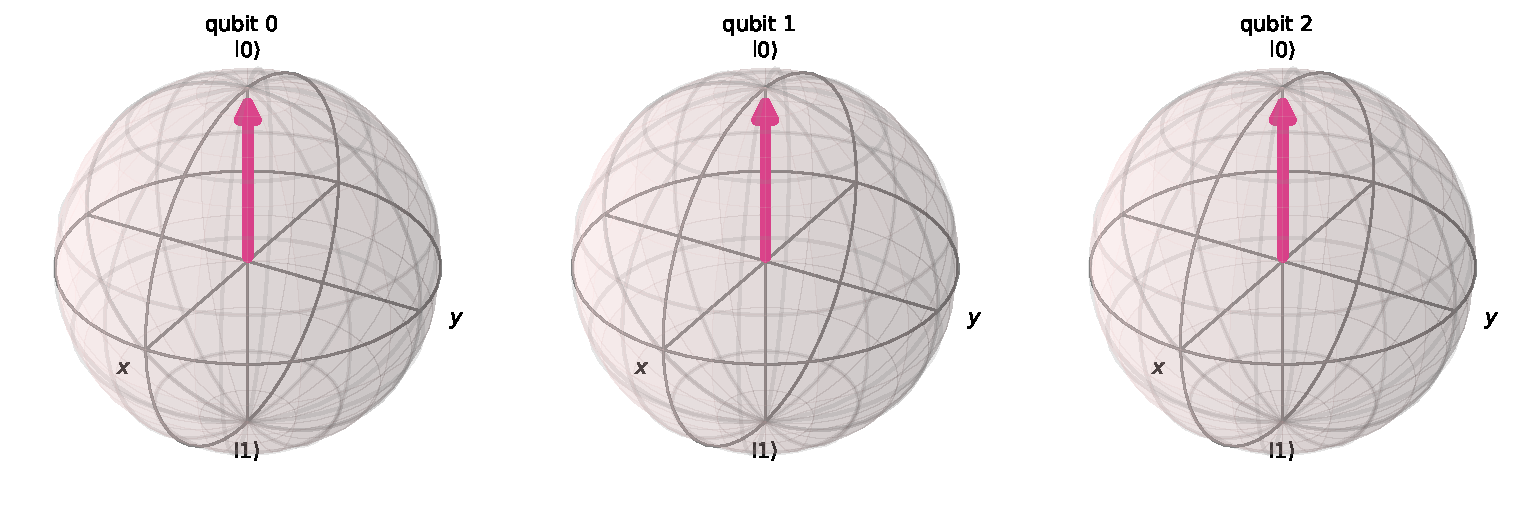
\includegraphics[keepaspectratio]{apostila_files/figure-pdf/cell-65-output-1.pdf}}

\pandocbounded{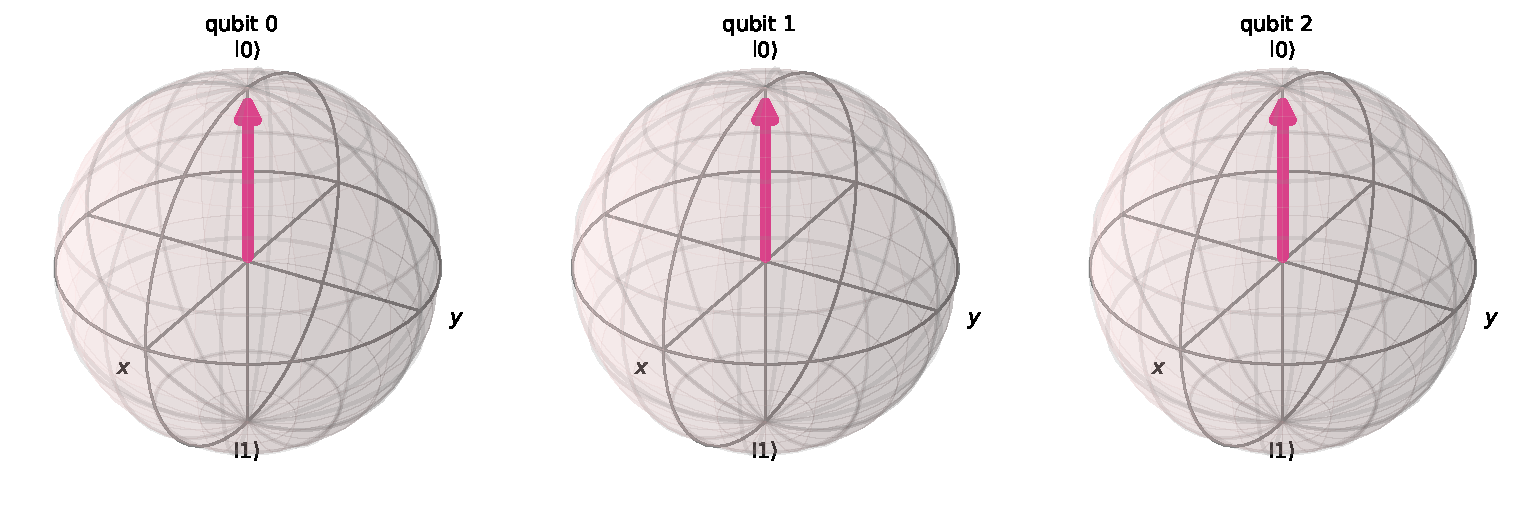
\includegraphics[keepaspectratio]{apostila_files/figure-pdf/cell-65-output-2.pdf}}

\subsubsection{🔹 Etapa 1: Preparar o estado a teletransportar (X no
qubit
0)}\label{etapa-1-preparar-o-estado-a-teletransportar-x-no-qubit-0}

\begin{Shaded}
\begin{Highlighting}[]
\CommentTok{\# Aplicar X no qubit 0 (preparar |1⟩)}
\NormalTok{final\_circuit.x(}\DecValTok{0}\NormalTok{)}
\NormalTok{final\_circuit.barrier()}

\CommentTok{\# Visualizar estado após X}
\NormalTok{state\_1 }\OperatorTok{=}\NormalTok{ Statevector.from\_instruction(final\_circuit)}
\BuiltInTok{print}\NormalTok{(}\StringTok{"Estado: |100⟩ (qubit 0 preparado em |1⟩)"}\NormalTok{)}
\BuiltInTok{print}\NormalTok{(state\_1)}
\NormalTok{final\_circuit.draw(}\StringTok{\textquotesingle{}mpl\textquotesingle{}}\NormalTok{)}
\end{Highlighting}
\end{Shaded}

\begin{verbatim}
Estado: |100⟩ (qubit 0 preparado em |1⟩)
Statevector([0.+0.j, 1.+0.j, 0.+0.j, 0.+0.j, 0.+0.j, 0.+0.j, 0.+0.j,
             0.+0.j],
            dims=(2, 2, 2))
\end{verbatim}

\pandocbounded{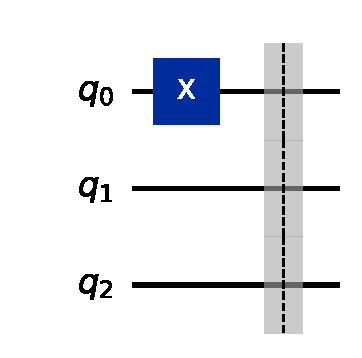
\includegraphics[keepaspectratio]{apostila_files/figure-pdf/cell-66-output-2.pdf}}

\pandocbounded{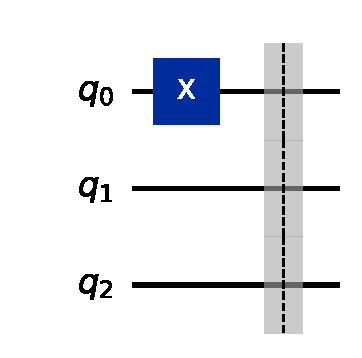
\includegraphics[keepaspectratio]{apostila_files/figure-pdf/cell-66-output-3.pdf}}

\begin{verbatim}
Estado: |100⟩ (qubit 0 preparado em |1⟩)
Statevector([0.+0.j, 1.+0.j, 0.+0.j, 0.+0.j, 0.+0.j, 0.+0.j, 0.+0.j,
             0.+0.j],
            dims=(2, 2, 2))
\end{verbatim}

\begin{Shaded}
\begin{Highlighting}[]
\NormalTok{plot\_bloch\_multivector(state\_1)}
\end{Highlighting}
\end{Shaded}

\pandocbounded{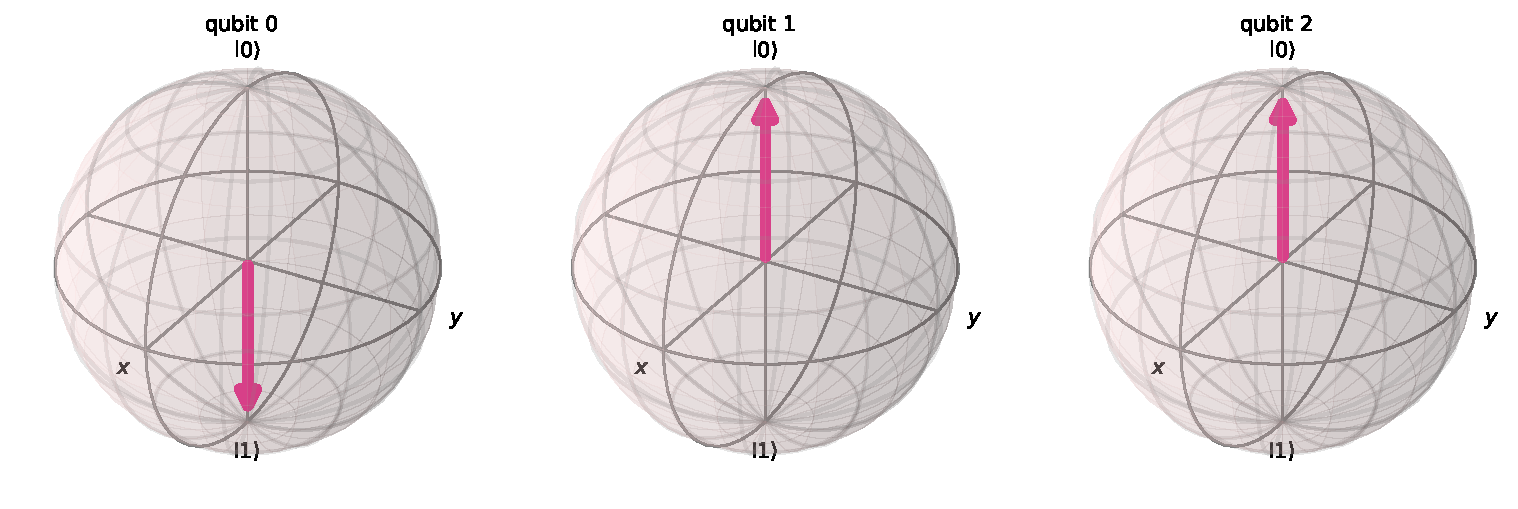
\includegraphics[keepaspectratio]{apostila_files/figure-pdf/cell-67-output-1.pdf}}

\pandocbounded{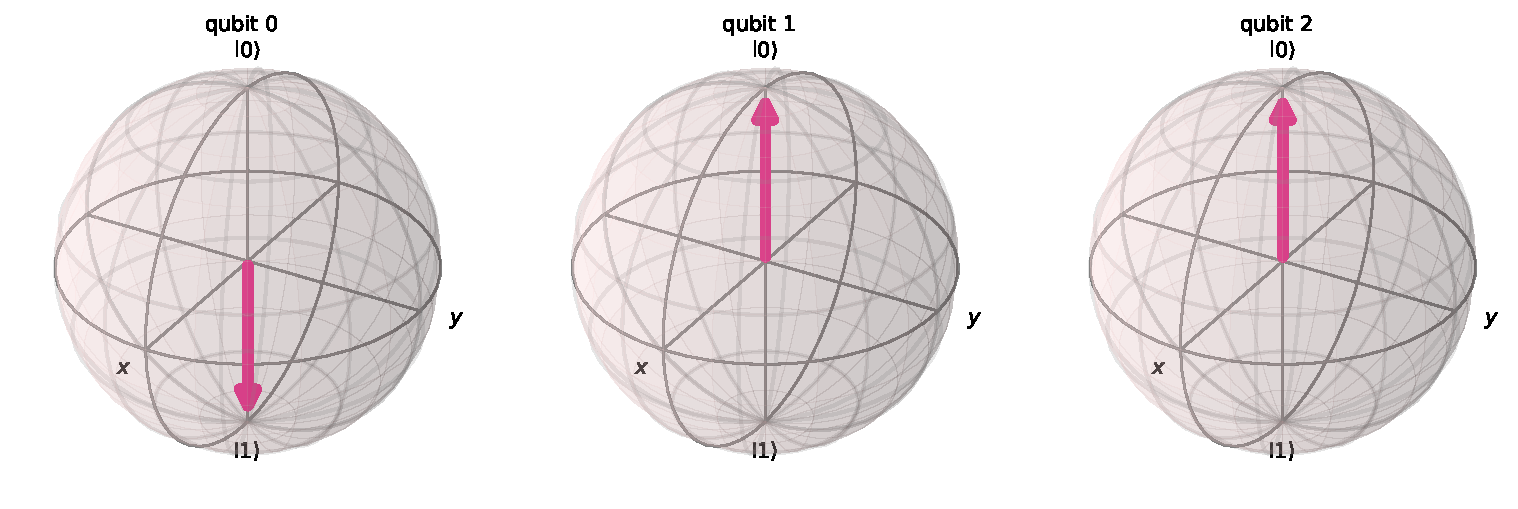
\includegraphics[keepaspectratio]{apostila_files/figure-pdf/cell-67-output-2.pdf}}

\subsubsection{🔹 Etapa 2: Criar par de Bell (H + CNOT nos qubits 1 e
2)}\label{etapa-2-criar-par-de-bell-h-cnot-nos-qubits-1-e-2}

\begin{Shaded}
\begin{Highlighting}[]
\CommentTok{\# Criar par de Bell entre qubits 1 e 2}
\NormalTok{final\_circuit.h(}\DecValTok{1}\NormalTok{)}
\NormalTok{final\_circuit.cx(}\DecValTok{1}\NormalTok{, }\DecValTok{2}\NormalTok{)}

\CommentTok{\# Visualizar estado após criar par de Bell}
\NormalTok{state\_2 }\OperatorTok{=}\NormalTok{ Statevector.from\_instruction(final\_circuit)}
\BuiltInTok{print}\NormalTok{(}\StringTok{"Estado: 1/√2(|100⟩ + |111⟩) {-} qubits 1 e 2 emaranhados"}\NormalTok{)}
\BuiltInTok{print}\NormalTok{(state\_2)}
\NormalTok{final\_circuit.draw(}\StringTok{\textquotesingle{}mpl\textquotesingle{}}\NormalTok{)}
\end{Highlighting}
\end{Shaded}

\begin{verbatim}
Estado: 1/√2(|100⟩ + |111⟩) - qubits 1 e 2 emaranhados
Statevector([0.        +0.j, 0.70710678+0.j, 0.        +0.j,
             0.        +0.j, 0.        +0.j, 0.        +0.j,
             0.        +0.j, 0.70710678+0.j],
            dims=(2, 2, 2))
\end{verbatim}

\pandocbounded{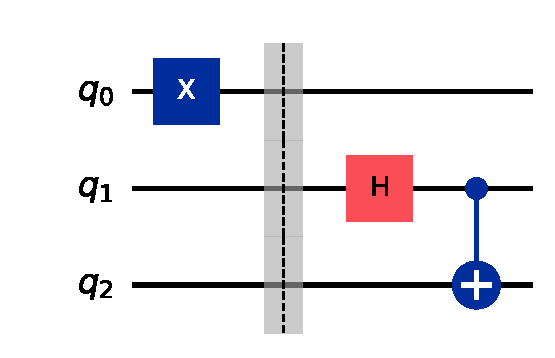
\includegraphics[keepaspectratio]{apostila_files/figure-pdf/cell-68-output-2.pdf}}

\pandocbounded{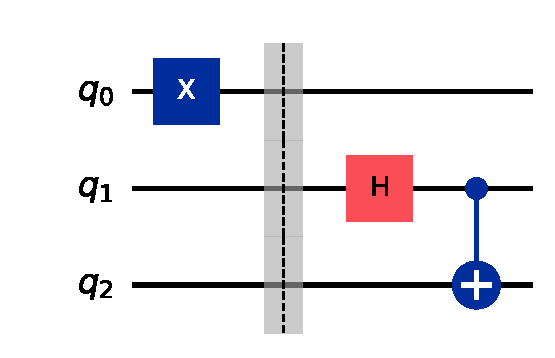
\includegraphics[keepaspectratio]{apostila_files/figure-pdf/cell-68-output-3.pdf}}

\begin{verbatim}
Estado: 1/√2(|100⟩ + |111⟩) - qubits 1 e 2 emaranhados
Statevector([0.        +0.j, 0.70710678+0.j, 0.        +0.j,
             0.        +0.j, 0.        +0.j, 0.        +0.j,
             0.        +0.j, 0.70710678+0.j],
            dims=(2, 2, 2))
\end{verbatim}

\begin{Shaded}
\begin{Highlighting}[]
\BuiltInTok{print}\NormalTok{(}\StringTok{"}\CharTok{\textbackslash{}n}\StringTok{🌐 Q{-}Sphere {-} Visualizando o emaranhamento:"}\NormalTok{)}
\NormalTok{plot\_state\_qsphere(state\_2)}
\end{Highlighting}
\end{Shaded}

\begin{verbatim}

🌐 Q-Sphere - Visualizando o emaranhamento:
\end{verbatim}

\pandocbounded{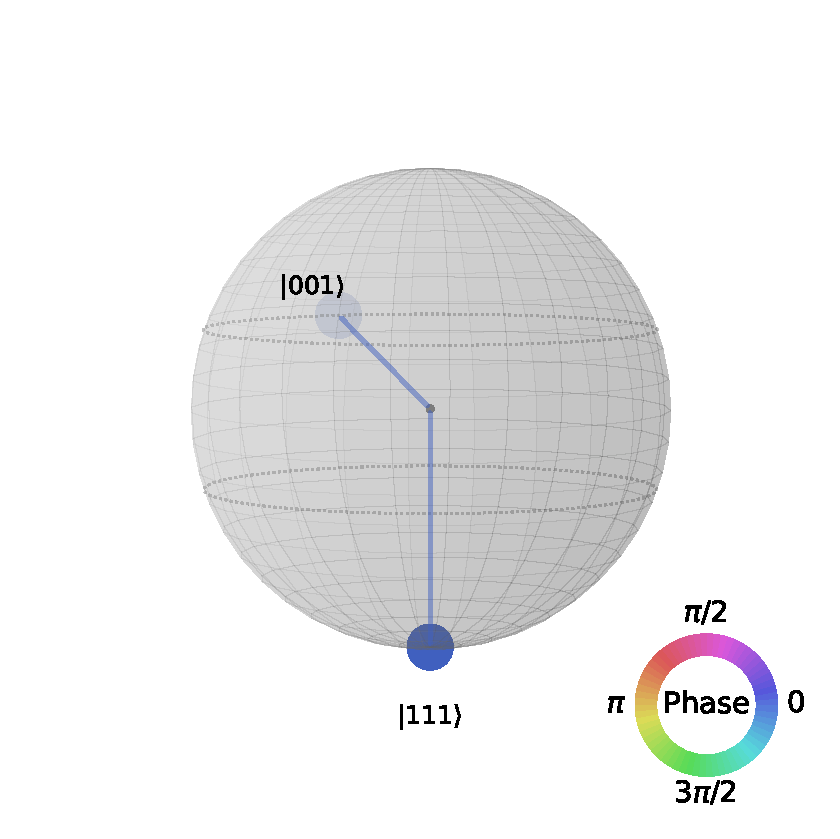
\includegraphics[keepaspectratio]{apostila_files/figure-pdf/cell-69-output-2.pdf}}

\pandocbounded{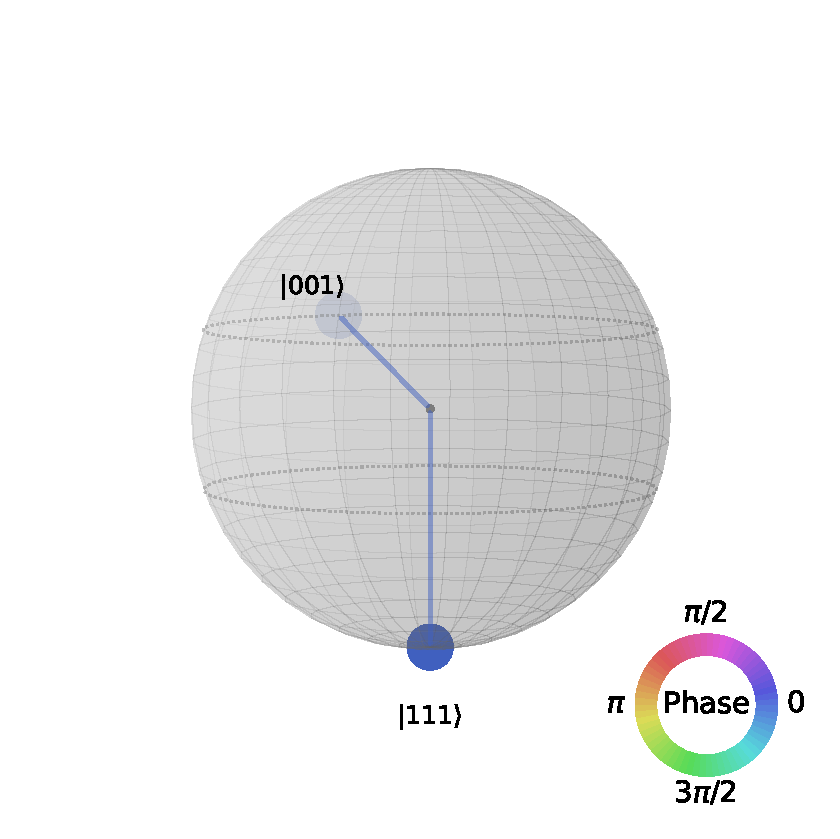
\includegraphics[keepaspectratio]{apostila_files/figure-pdf/cell-69-output-3.pdf}}

\begin{verbatim}

🌐 Q-Sphere - Visualizando o emaranhamento:
\end{verbatim}

\begin{Shaded}
\begin{Highlighting}[]
\NormalTok{plot\_bloch\_multivector(state\_2)}
\end{Highlighting}
\end{Shaded}

\pandocbounded{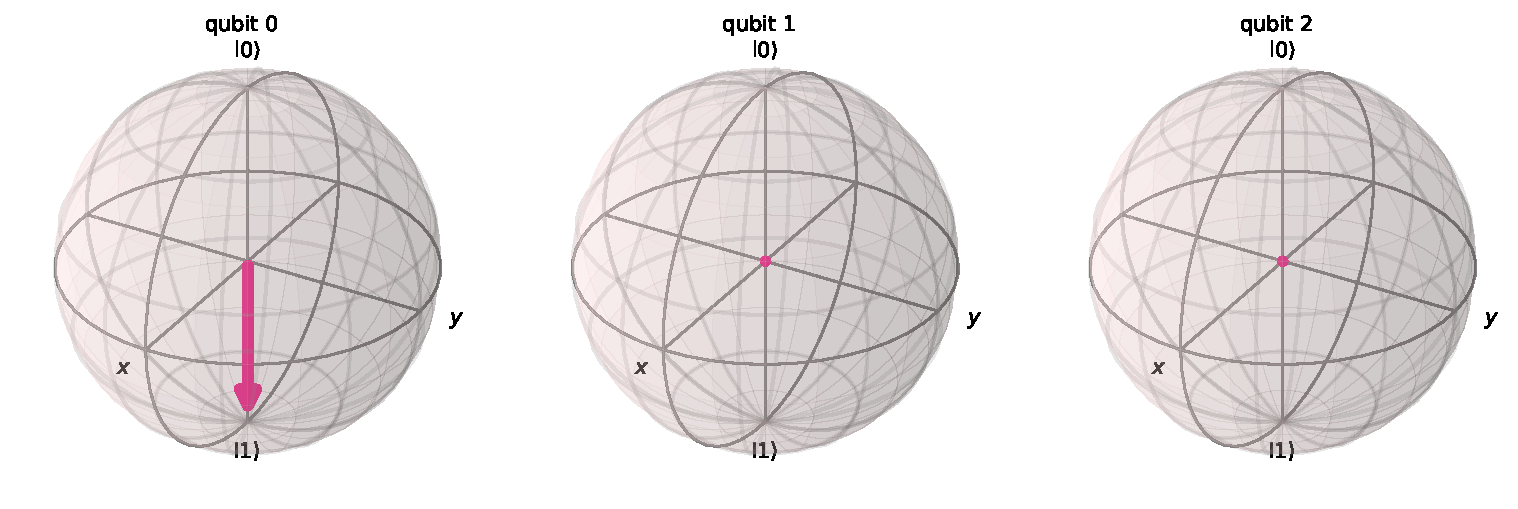
\includegraphics[keepaspectratio]{apostila_files/figure-pdf/cell-70-output-1.pdf}}

\pandocbounded{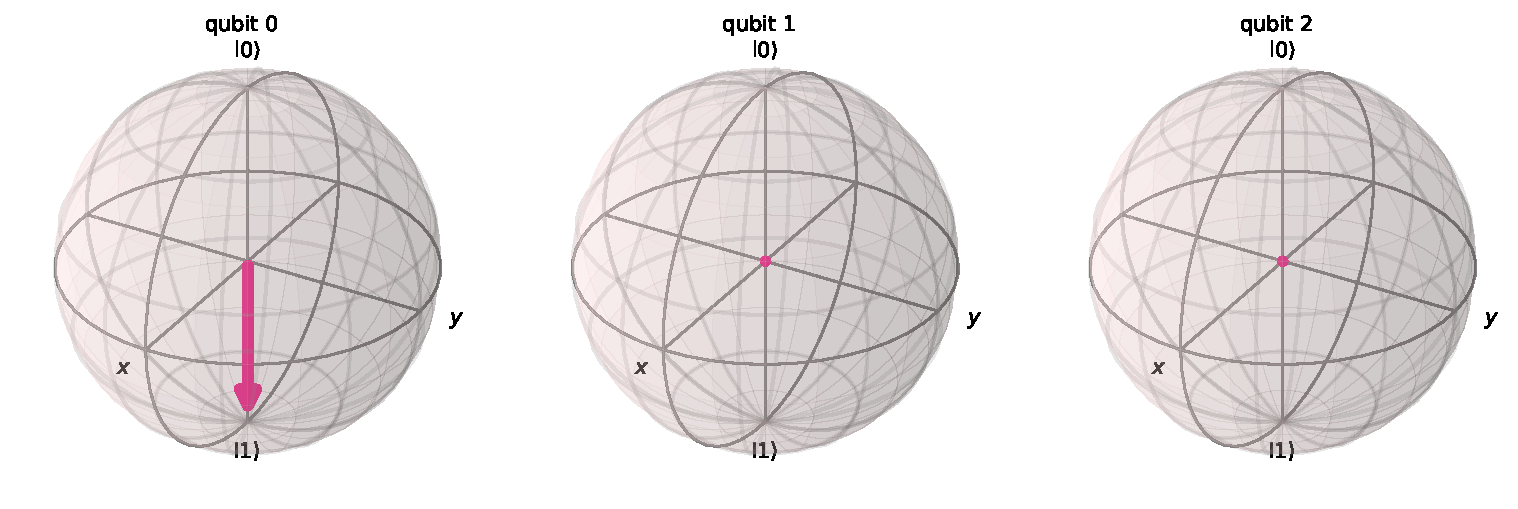
\includegraphics[keepaspectratio]{apostila_files/figure-pdf/cell-70-output-2.pdf}}

\subsubsection{🔹 Etapa 3: Medição de Bell (CNOT + H nos qubits de
Alice)}\label{etapa-3-mediuxe7uxe3o-de-bell-cnot-h-nos-qubits-de-alice}

\begin{Shaded}
\begin{Highlighting}[]
\CommentTok{\# Aplicar medição de Bell (sem as medições clássicas)}
\NormalTok{final\_circuit.cx(}\DecValTok{0}\NormalTok{, }\DecValTok{1}\NormalTok{)}
\NormalTok{final\_circuit.h(}\DecValTok{0}\NormalTok{)}
\NormalTok{final\_circuit.barrier()}

\CommentTok{\# Visualizar estado após medição de Bell}
\NormalTok{state\_3 }\OperatorTok{=}\NormalTok{ Statevector.from\_instruction(final\_circuit)}
\BuiltInTok{print}\NormalTok{(}\StringTok{"Estado: 1/2(|010⟩ {-} |110⟩ + |001⟩ {-} |101⟩) {-} 3 qubits emaranhados"}\NormalTok{)}
\BuiltInTok{print}\NormalTok{(state\_3)}
\NormalTok{final\_circuit.draw(}\StringTok{\textquotesingle{}mpl\textquotesingle{}}\NormalTok{)}
\end{Highlighting}
\end{Shaded}

\begin{verbatim}
Estado: 1/2(|010⟩ - |110⟩ + |001⟩ - |101⟩) - 3 qubits emaranhados
Statevector([ 0. +0.j,  0. +0.j,  0.5+0.j, -0.5+0.j,  0.5+0.j, -0.5+0.j,
              0. +0.j,  0. +0.j],
            dims=(2, 2, 2))
\end{verbatim}

\pandocbounded{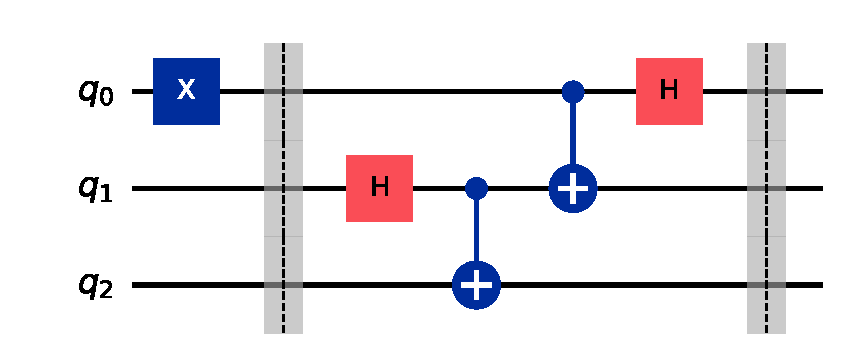
\includegraphics[keepaspectratio]{apostila_files/figure-pdf/cell-71-output-2.pdf}}

\pandocbounded{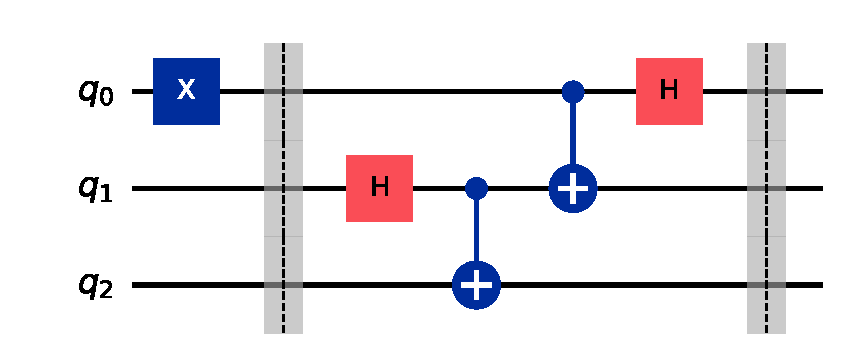
\includegraphics[keepaspectratio]{apostila_files/figure-pdf/cell-71-output-3.pdf}}

\begin{verbatim}
Estado: 1/2(|010⟩ - |110⟩ + |001⟩ - |101⟩) - 3 qubits emaranhados
Statevector([ 0. +0.j,  0. +0.j,  0.5+0.j, -0.5+0.j,  0.5+0.j, -0.5+0.j,
              0. +0.j,  0. +0.j],
            dims=(2, 2, 2))
\end{verbatim}

\begin{Shaded}
\begin{Highlighting}[]
\BuiltInTok{print}\NormalTok{(}\StringTok{"}\CharTok{\textbackslash{}n}\StringTok{🌐 Q{-}Sphere {-} Superposição dos 4 cenários possíveis:"}\NormalTok{)}
\NormalTok{plot\_state\_qsphere(state\_3)}
\end{Highlighting}
\end{Shaded}

\begin{verbatim}

🌐 Q-Sphere - Superposição dos 4 cenários possíveis:
\end{verbatim}

\pandocbounded{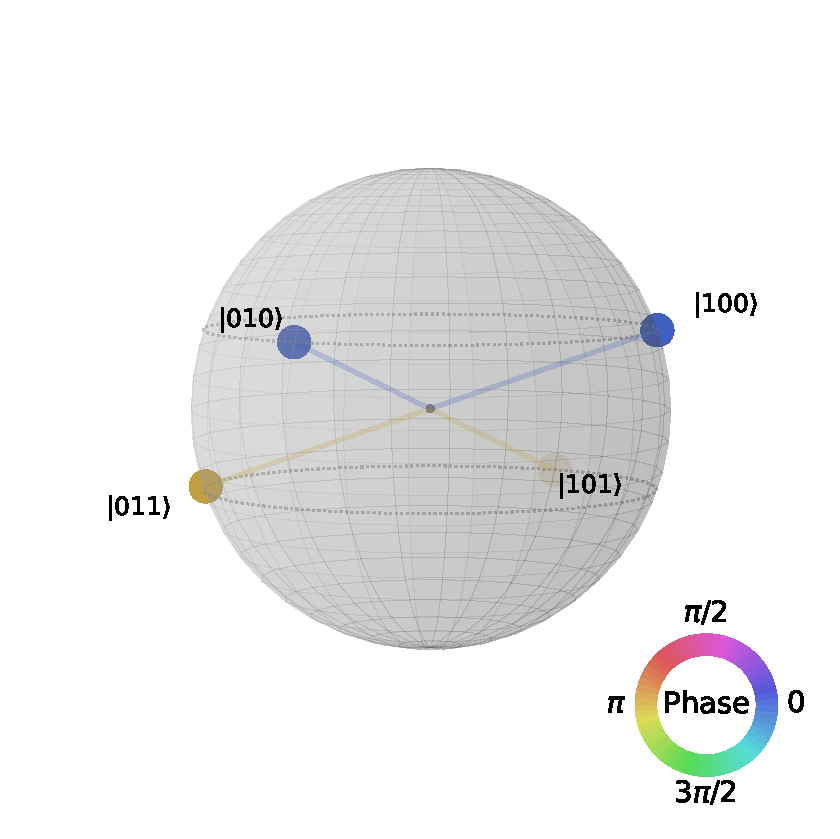
\includegraphics[keepaspectratio]{apostila_files/figure-pdf/cell-72-output-2.pdf}}

\pandocbounded{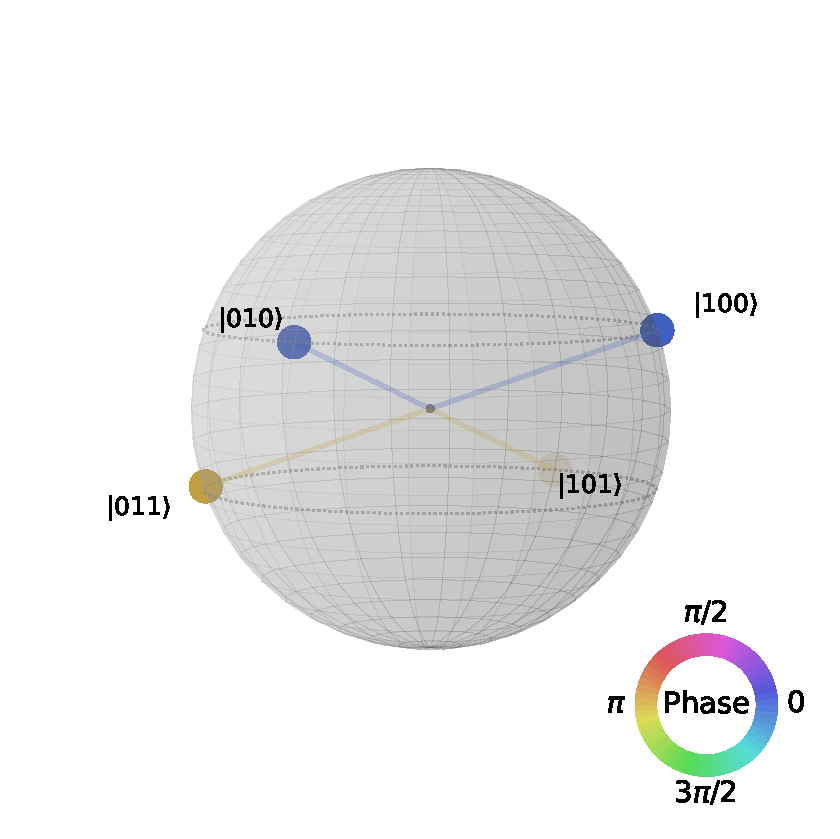
\includegraphics[keepaspectratio]{apostila_files/figure-pdf/cell-72-output-3.pdf}}

\begin{verbatim}

🌐 Q-Sphere - Superposição dos 4 cenários possíveis:
\end{verbatim}

\begin{Shaded}
\begin{Highlighting}[]
\NormalTok{plot\_bloch\_multivector(state\_3)}
\end{Highlighting}
\end{Shaded}

\pandocbounded{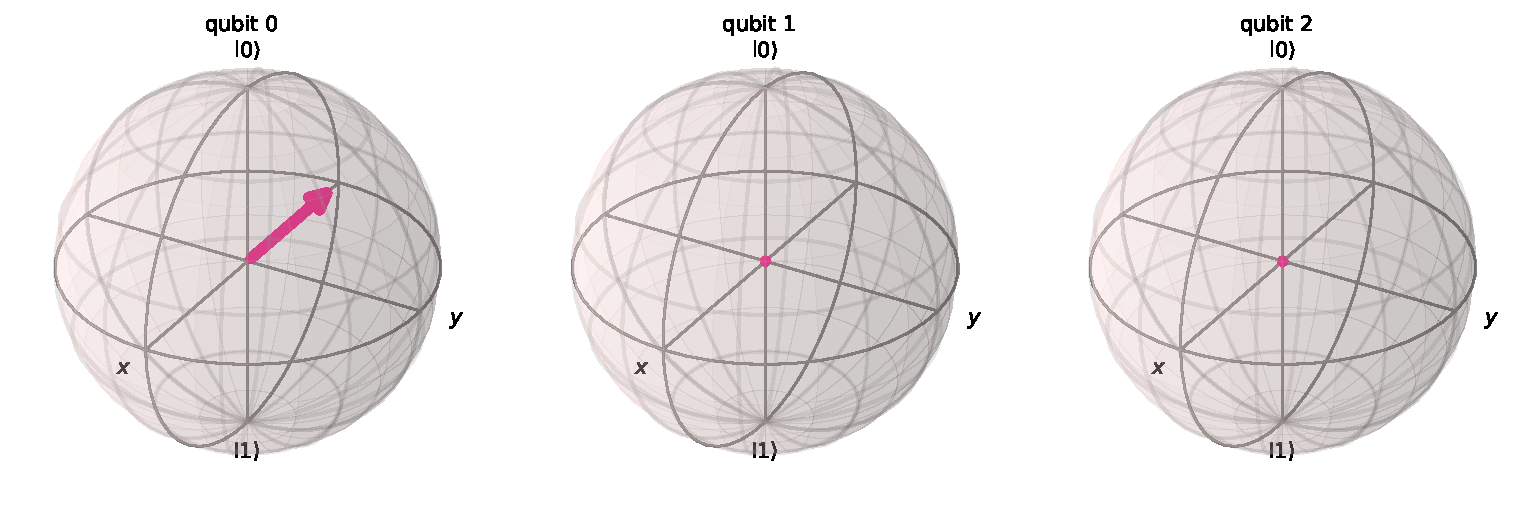
\includegraphics[keepaspectratio]{apostila_files/figure-pdf/cell-73-output-1.pdf}}

\pandocbounded{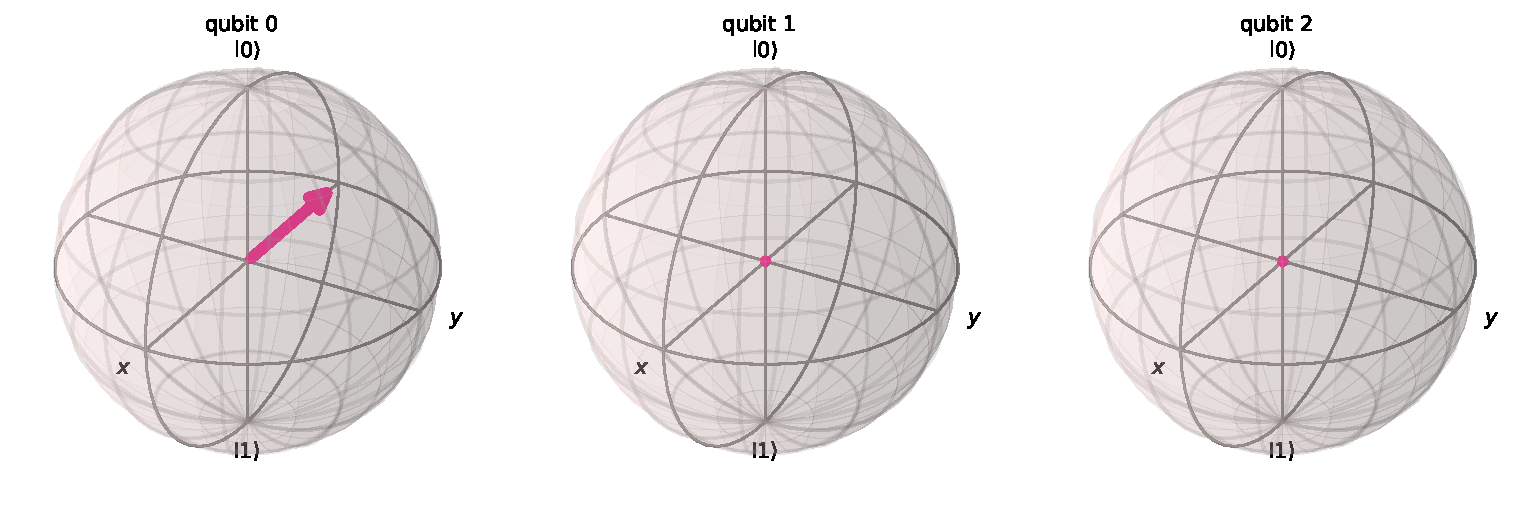
\includegraphics[keepaspectratio]{apostila_files/figure-pdf/cell-73-output-2.pdf}}

\subsubsection{📊 Resumo do Estado Final (antes das correções de
Bob)}\label{resumo-do-estado-final-antes-das-correuxe7uxf5es-de-bob}

\begin{Shaded}
\begin{Highlighting}[]
\CommentTok{\# Estado completo antes das correções de Bob}
\NormalTok{state\_final }\OperatorTok{=}\NormalTok{ Statevector.from\_instruction(final\_circuit)}
\BuiltInTok{print}\NormalTok{(}\StringTok{"Estado completo antes das correções:"}\NormalTok{)}
\BuiltInTok{print}\NormalTok{(state\_final)}
\BuiltInTok{print}\NormalTok{(}\StringTok{"}\CharTok{\textbackslash{}n}\StringTok{Este estado representa os 4 cenários possíveis com igual probabilidade (25}\SpecialCharTok{\% c}\StringTok{ada)"}\NormalTok{)}

\CommentTok{\# Bloch sphere}
\NormalTok{plot\_bloch\_multivector(state\_final)}
\end{Highlighting}
\end{Shaded}

\begin{verbatim}
Estado completo antes das correções:
Statevector([ 0. +0.j,  0. +0.j,  0.5+0.j, -0.5+0.j,  0.5+0.j, -0.5+0.j,
              0. +0.j,  0. +0.j],
            dims=(2, 2, 2))

Este estado representa os 4 cenários possíveis com igual probabilidade (25% cada)
\end{verbatim}

\pandocbounded{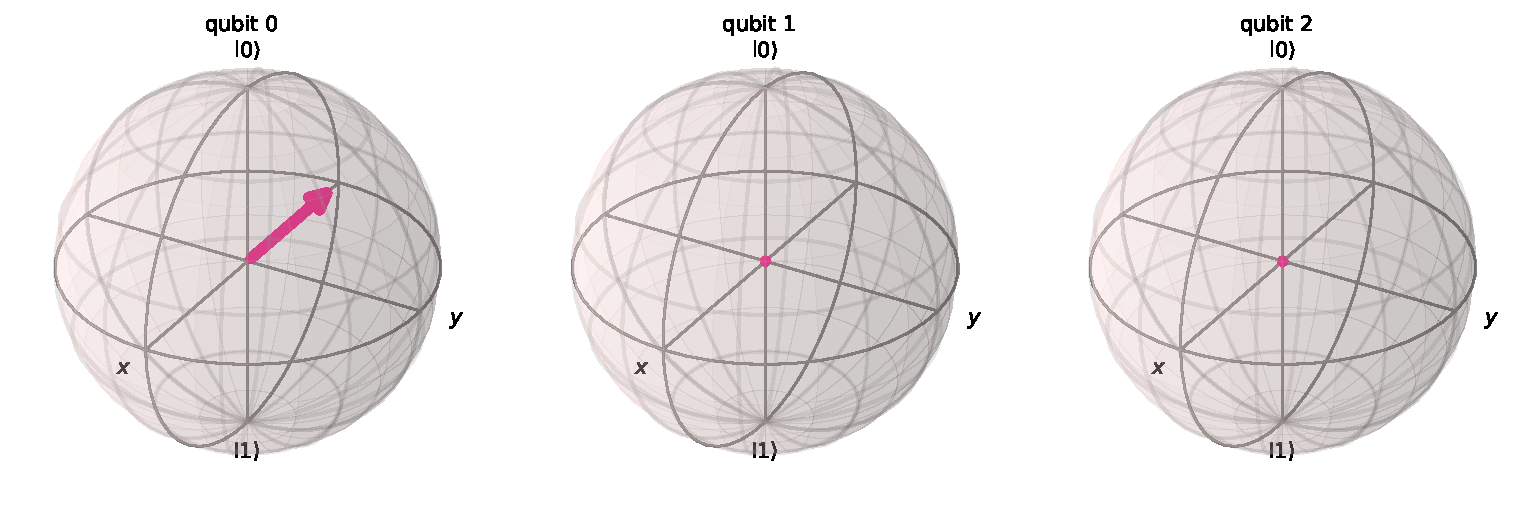
\includegraphics[keepaspectratio]{apostila_files/figure-pdf/cell-74-output-2.pdf}}

\pandocbounded{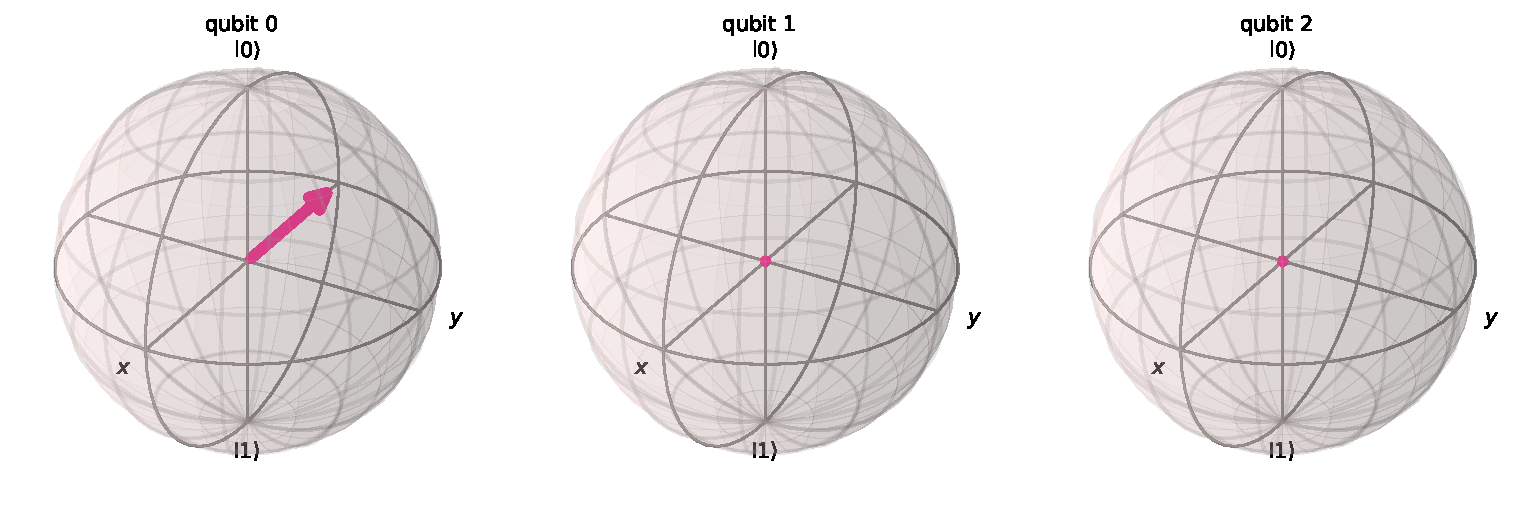
\includegraphics[keepaspectratio]{apostila_files/figure-pdf/cell-74-output-3.pdf}}

\begin{verbatim}
Estado completo antes das correções:
Statevector([ 0. +0.j,  0. +0.j,  0.5+0.j, -0.5+0.j,  0.5+0.j, -0.5+0.j,
              0. +0.j,  0. +0.j],
            dims=(2, 2, 2))

Este estado representa os 4 cenários possíveis com igual probabilidade (25% cada)
\end{verbatim}

\begin{Shaded}
\begin{Highlighting}[]
\BuiltInTok{print}\NormalTok{(}\StringTok{"}\CharTok{\textbackslash{}n}\StringTok{🏙️ State City {-} Estrutura completa do estado emaranhado:"}\NormalTok{)}
\NormalTok{plot\_state\_city(state\_final)}
\end{Highlighting}
\end{Shaded}

\begin{verbatim}

🏙️ State City - Estrutura completa do estado emaranhado:
\end{verbatim}

\pandocbounded{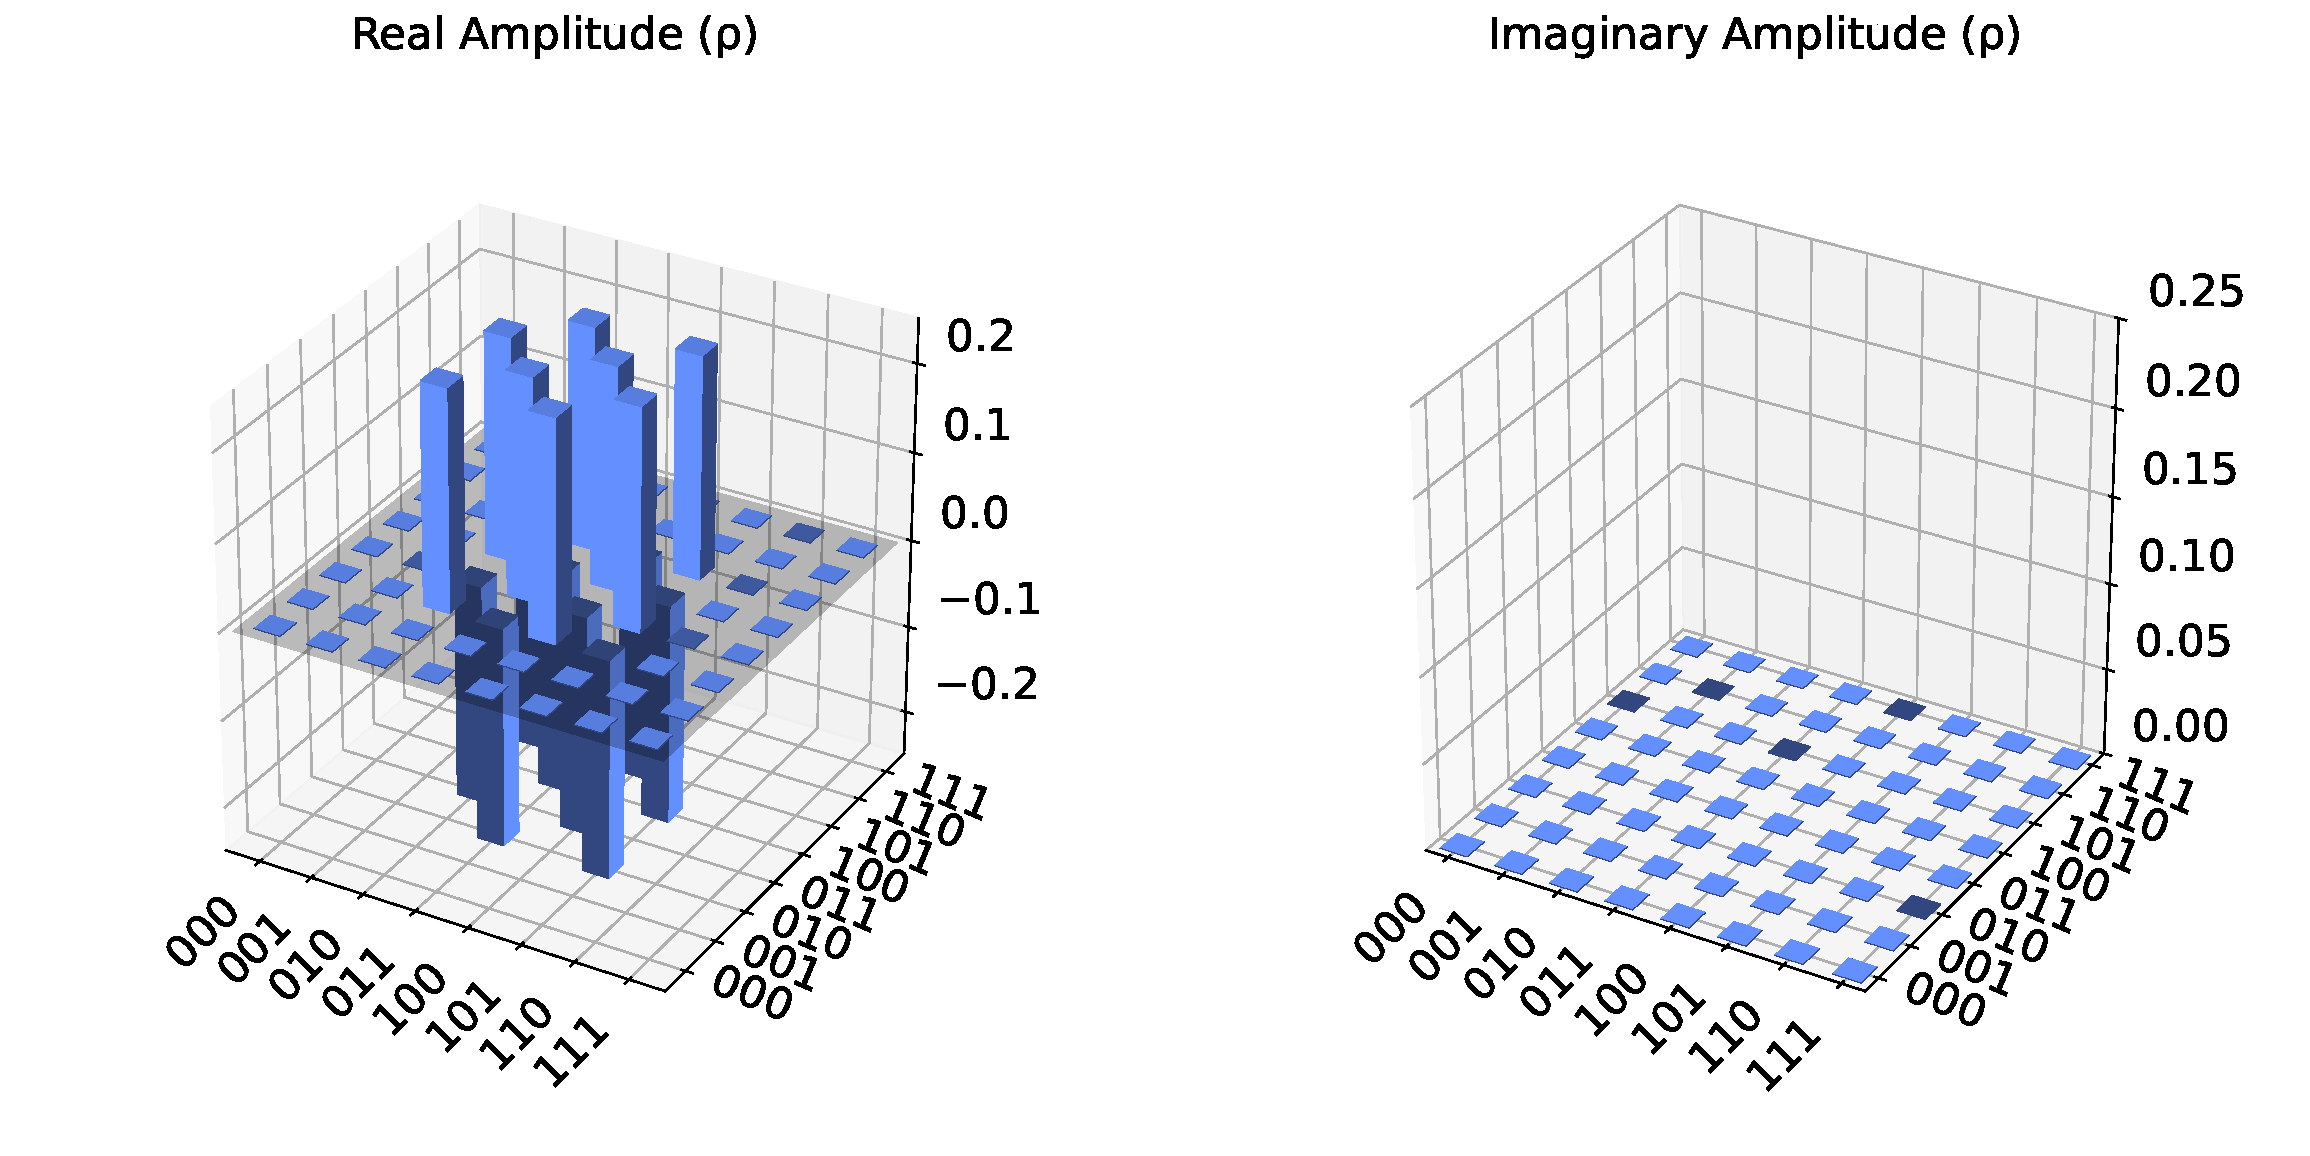
\includegraphics[keepaspectratio]{apostila_files/figure-pdf/cell-75-output-2.pdf}}

\pandocbounded{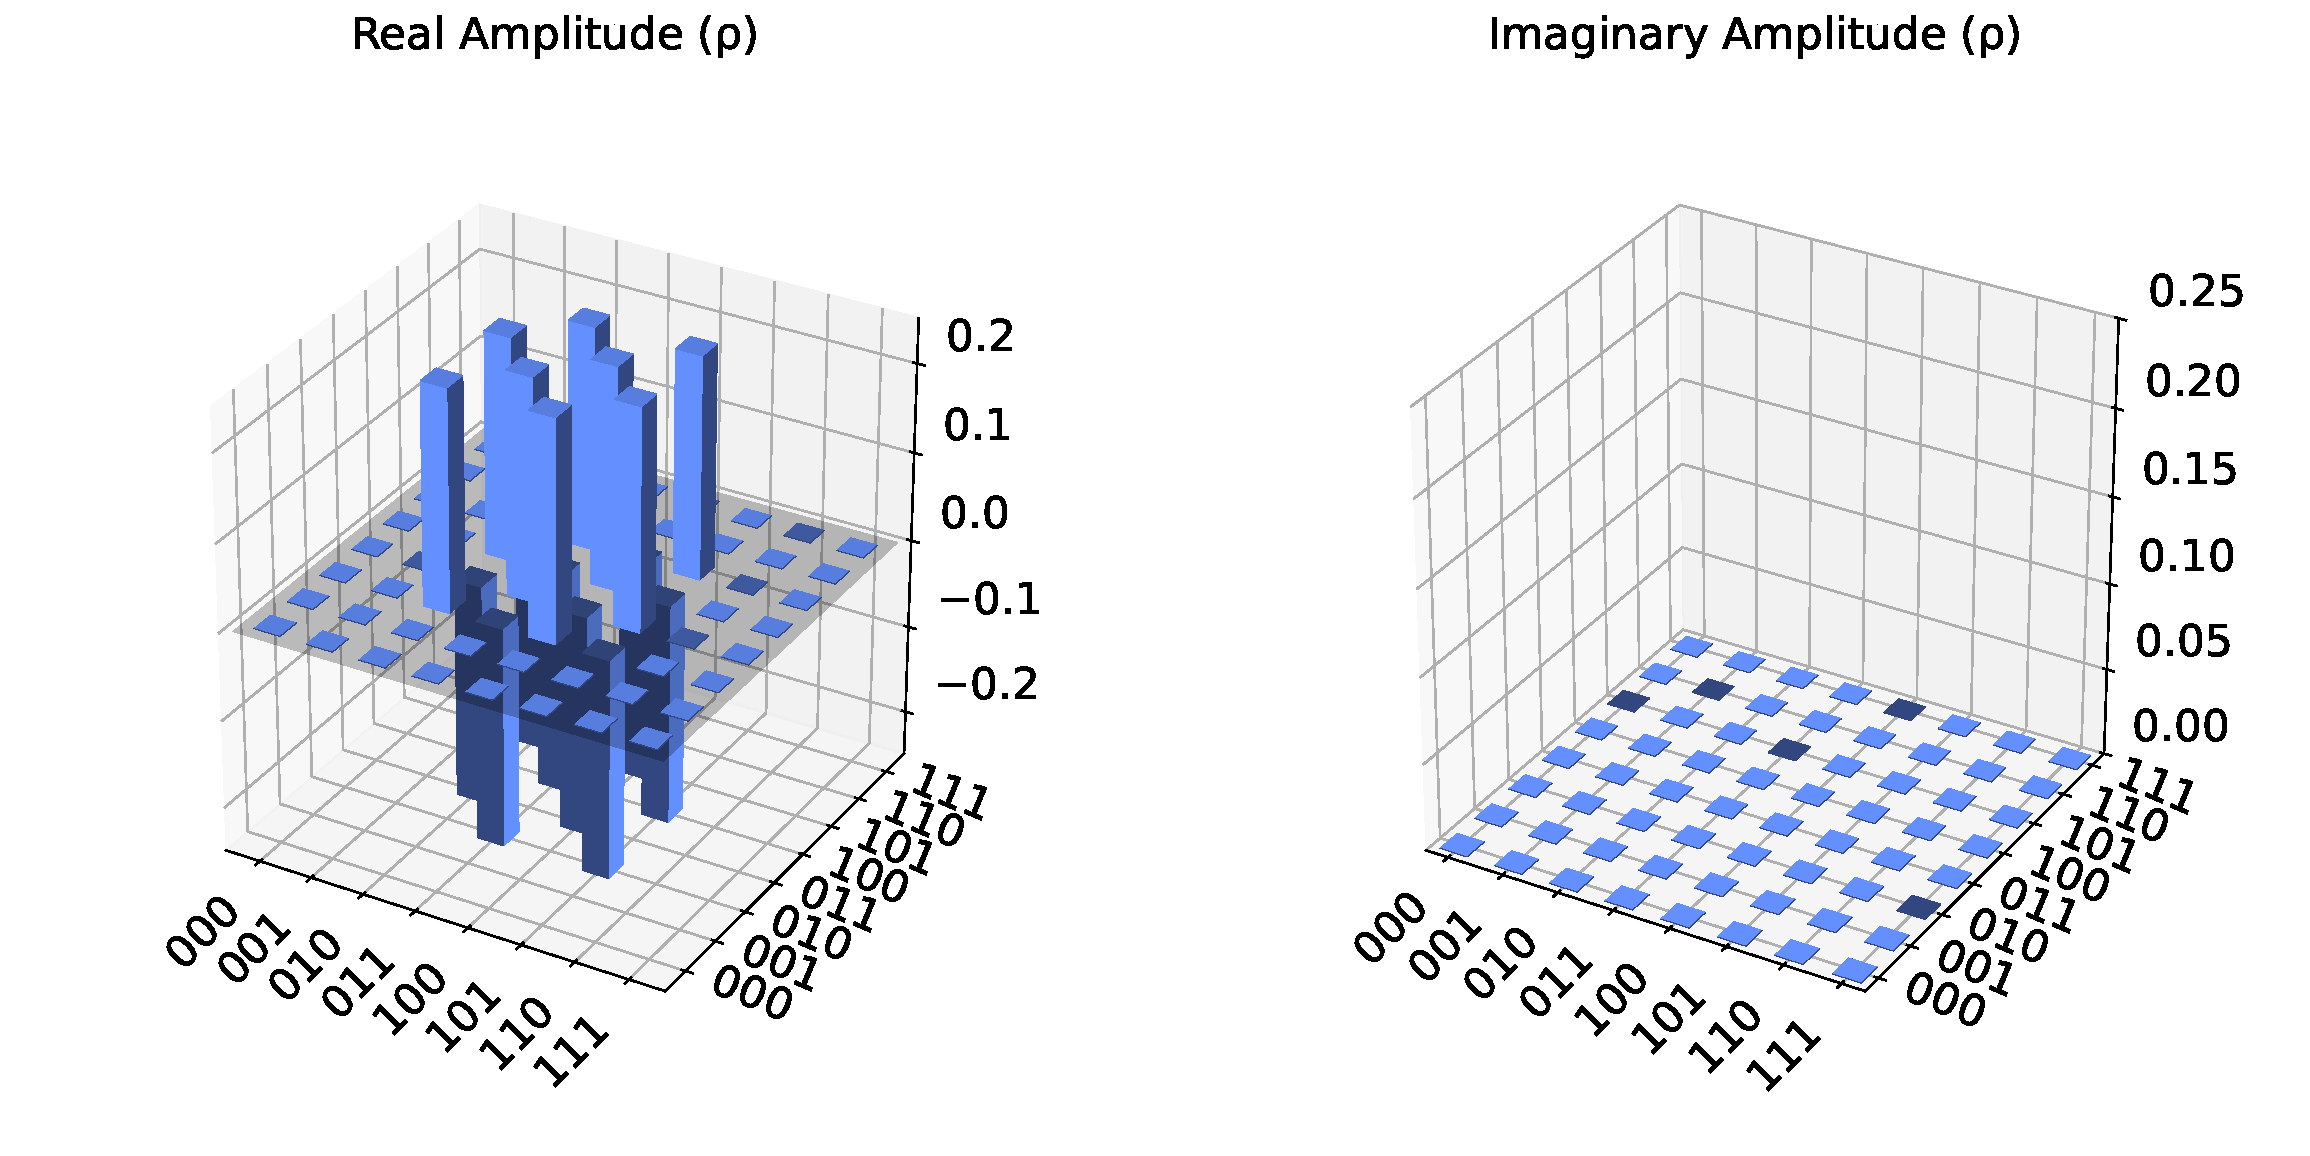
\includegraphics[keepaspectratio]{apostila_files/figure-pdf/cell-75-output-3.pdf}}

\begin{verbatim}

🏙️ State City - Estrutura completa do estado emaranhado:
\end{verbatim}

\begin{Shaded}
\begin{Highlighting}[]
\BuiltInTok{print}\NormalTok{(}\StringTok{"}\CharTok{\textbackslash{}n}\StringTok{🌐 Q{-}Sphere {-} Todas as amplitudes:"}\NormalTok{)}
\NormalTok{plot\_state\_qsphere(state\_final)}
\end{Highlighting}
\end{Shaded}

\begin{verbatim}

🌐 Q-Sphere - Todas as amplitudes:
\end{verbatim}

\pandocbounded{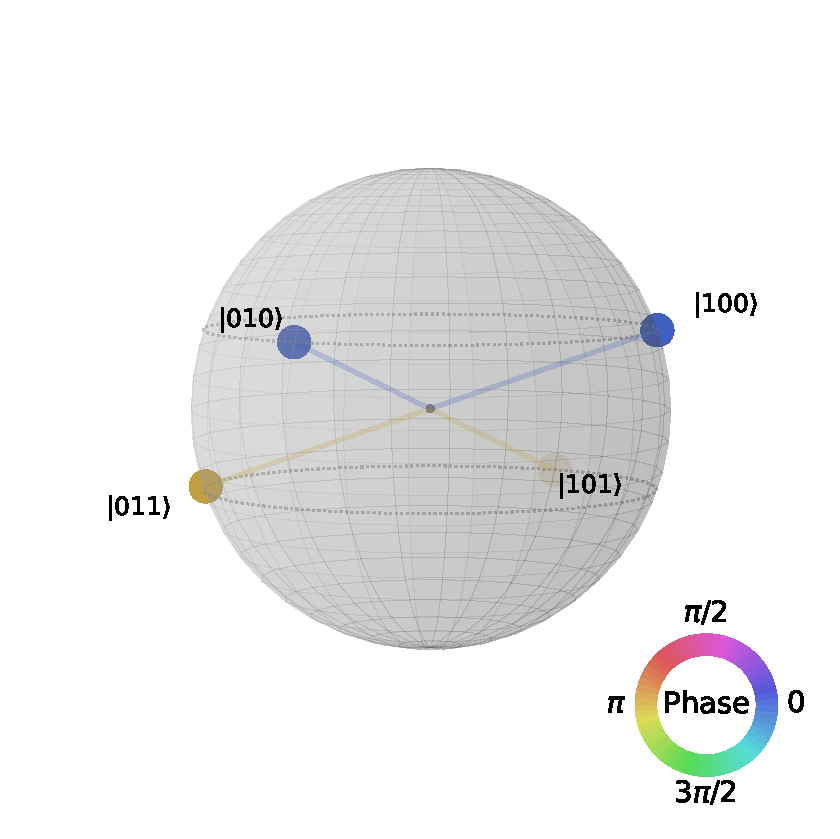
\includegraphics[keepaspectratio]{apostila_files/figure-pdf/cell-76-output-2.pdf}}

\pandocbounded{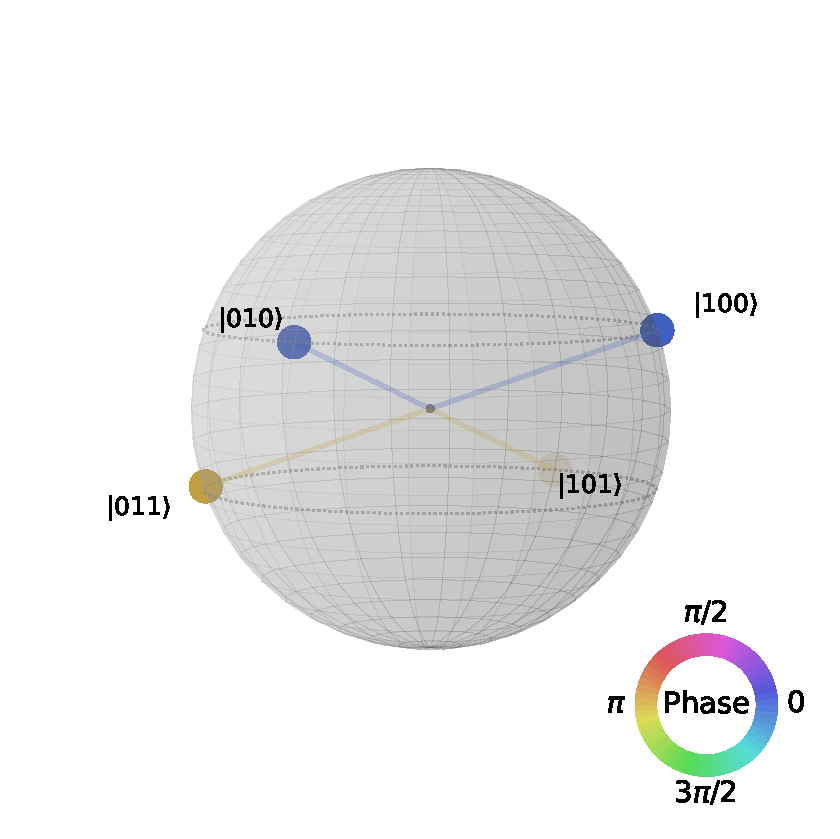
\includegraphics[keepaspectratio]{apostila_files/figure-pdf/cell-76-output-3.pdf}}

\begin{verbatim}

🌐 Q-Sphere - Todas as amplitudes:
\end{verbatim}

\subsection{📐 Interpretação Matemática do
Estado}\label{interpretauxe7uxe3o-matemuxe1tica-do-estado}

Este estado é uma \textbf{superposição de 4 cenários} correspondentes
aos 4 possíveis resultados da medição de Bell de Alice. Cada cenário tem
25\% de probabilidade e deixa o qubit de Bob em um estado relacionado ao
estado original \(|1\rangle\):

\textbf{Probabilidades:}
\[P(|010\rangle) = \left|\frac{1}{2}\right|^2 = \frac{1}{4} = 25\%\]

E assim por diante para cada termo. O estado está perfeitamente
balanceado entre as 4 possibilidades!

Estado após a medição de Bell (antes das correções quânticas):

\subsection{🎯 Teste Final: Funcionou?}\label{teste-final-funcionou}

Vamos executar o circuito completo 1000 vezes e ver os resultados!

\textbf{Como ler os resultados:} - Formato da Qiskit:
\texttt{c{[}2{]}c{[}1{]}c{[}0{]}} (ordem reversa - confuso, eu sei!) - O
que queremos ver: \textbf{\texttt{100}} - c{[}2{]} = \textbf{1} → Bob
recebeu \textbar1⟩ ✅ - c{[}1{]} = \textbf{0} → Uma das medições de
Alice - c{[}0{]} = \textbf{0} → Outra medição de Alice

💡 \textbf{Se você ver principalmente `100':} PARABÉNS! O teletransporte
funcionou!

\begin{Shaded}
\begin{Highlighting}[]
\CommentTok{\# Executar o circuito completo e verificar os resultados}
\ImportTok{from}\NormalTok{ qiskit\_aer }\ImportTok{import}\NormalTok{ AerSimulator}

\CommentTok{\# Criar simulador}
\NormalTok{simulator }\OperatorTok{=}\NormalTok{ AerSimulator()}

\CommentTok{\# Executar o circuito}
\NormalTok{job }\OperatorTok{=}\NormalTok{ simulator.run(circuit, shots}\OperatorTok{=}\DecValTok{1000}\NormalTok{)}
\NormalTok{result }\OperatorTok{=}\NormalTok{ job.result()}
\NormalTok{counts }\OperatorTok{=}\NormalTok{ result.get\_counts()}

\BuiltInTok{print}\NormalTok{(}\StringTok{"Resultados das medições (1000 execuções):"}\NormalTok{)}
\BuiltInTok{print}\NormalTok{(counts)}
\BuiltInTok{print}\NormalTok{(}\StringTok{"}\CharTok{\textbackslash{}n}\StringTok{O resultado esperado é \textquotesingle{}100\textquotesingle{} (qubit 2 = |1⟩, demonstrando o teletransporte)"}\NormalTok{)}
\end{Highlighting}
\end{Shaded}

\begin{verbatim}
Resultados das medições (1000 execuções):
{'101': 256, '100': 266, '110': 228, '111': 250}

O resultado esperado é '100' (qubit 2 = |1⟩, demonstrando o teletransporte)
\end{verbatim}

\begin{verbatim}
Resultados das medições (1000 execuções):
{'110': 255, '101': 248, '111': 259, '100': 238}

O resultado esperado é '100' (qubit 2 = |1⟩, demonstrando o teletransporte)
\end{verbatim}

\chapter{🎓 Recapitulando: O que
Aprendemos?}\label{recapitulando-o-que-aprendemos}

\section{✅ O Protocolo em 5 Passos}\label{o-protocolo-em-5-passos}

\begin{enumerate}
\def\labelenumi{\arabic{enumi}.}
\tightlist
\item
  \textbf{🎭 Preparação}: Alice criou o estado \textbar1⟩ no qubit 0
\item
  \textbf{⚡ Emaranhamento}: Criamos conexão quântica entre qubits 1 e 2
  (o ``telefone quântico'')
\item
  \textbf{🔗 Conexão}: Alice conectou seu qubit ao sistema emaranhado
\item
  \textbf{📞 Comunicação}: Alice mediu e enviou 2 bits clássicos para
  Bob
\item
  \textbf{🔧 Correção}: Bob usou essas informações para recuperar o
  estado original
\item
  \textbf{🎉 Resultado}: O qubit de Bob agora tem o estado \textbar1⟩!
\end{enumerate}

\section{📐 Resumo Matemático}\label{resumo-matemuxe1tico}

\textbf{Evolução do estado durante o protocolo:}

\begin{enumerate}
\def\labelenumi{\arabic{enumi}.}
\tightlist
\item
  \textbf{Inicial}: \(|000\rangle\)
\item
  \textbf{Após X}: \(|100\rangle\)
\item
  \textbf{Após H e CNOT (par de Bell)}:
  \(\frac{1}{\sqrt{2}}(|100\rangle + |111\rangle)\)
\item
  \textbf{Após medição de Bell}:
  \(\frac{1}{2}(|010\rangle - |110\rangle + |001\rangle - |101\rangle)\)
\item
  \textbf{Após medição de Alice}: Bob tem um de 4 estados possíveis
  (equiprováveis)
\item
  \textbf{Após correções de Bob}: \(|1\rangle\) (estado original
  teletransportado!)
\end{enumerate}

\textbf{A ``mágica'' está no emaranhamento:}

O estado de Bell
\(|\Phi^+\rangle = \frac{1}{\sqrt{2}}(|00\rangle + |11\rangle)\) cria
correlações quânticas que permitem que: - A informação seja
``distribuída'' entre os 3 qubits - Alice extraia informação clássica
através da medição - Bob use essa informação para reconstruir o estado
original

\textbf{Propriedade-chave:} Para qualquer estado inicial
\(|\psi\rangle = \alpha|0\rangle + \beta|1\rangle\), o protocolo
funciona SEM que Alice ou Bob conheçam \(\alpha\) e \(\beta\)!

\section{🤔 Perguntas Frequentes}\label{perguntas-frequentes}

\textbf{Q: Isso é teletransporte de verdade?} A: Sim! A informação
quântica foi transferida, mas o estado original foi destruído.

\textbf{Q: É instantâneo? Mais rápido que a luz?} A: NÃO! Bob precisa
receber a ligação de Alice (informação clássica), que viaja no máximo na
velocidade da luz.

\textbf{Q: Posso clonar um estado quântico assim?} A: NÃO! O estado
original de Alice foi destruído na medição (teorema da não-clonagem).

\textbf{Q: Por que isso é útil?} A: Comunicação quântica segura,
computação quântica distribuída, internet quântica!

\section{🎯 O Truque Fundamental}\label{o-truque-fundamental}

\textbf{Emaranhamento quântico} = A ``mágica'' que permite isso - Qubits
emaranhados ficam correlacionados instantaneamente - Mas ainda
precisamos de comunicação clássica para completar o protocolo - É a
combinação de ambos que torna o teletransporte possível!

\subsection{🚀 Próximos Passos}\label{pruxf3ximos-passos-1}

\begin{itemize}
\tightlist
\item
  Tente mudar o estado inicial (use H, Ry, etc. em vez de X)
\item
  Experimente teletransportar estados em superposição
\item
  Estude outros protocolos: superdense coding, criptografia quântica
  BB84
\end{itemize}

\newpage

\chapter{Módulo 8: Experimento de Interferência com
Hadamard}\label{muxf3dulo-8-experimento-de-interferuxeancia-com-hadamard}

\chapter{Aula 08 --- Experimento de Interferência com Hadamard
(Mach-Zehnder)}\label{aula-08-experimento-de-interferuxeancia-com-hadamard-mach-zehnder}

\section{Experimento de Interferência com Hadamard (Interferômetro de
Mach-Zehnder)}\label{experimento-de-interferuxeancia-com-hadamard-interferuxf4metro-de-mach-zehnder}

Você pode replicar esse experimento físico agora mesmo no Qiskit. É a
prova de que a porta Hadamard é reversível.

Matematicamente, aplicar dois Hadamards é igual a não fazer nada
(Identidade), pois as superposições se cancelam e voltam ao estado
original.

\begin{Shaded}
\begin{Highlighting}[]
\ImportTok{from}\NormalTok{ qiskit }\ImportTok{import}\NormalTok{ QuantumCircuit}
\ImportTok{from}\NormalTok{ qiskit.quantum\_info }\ImportTok{import}\NormalTok{ Statevector}
\ImportTok{from}\NormalTok{ qiskit.visualization }\ImportTok{import}\NormalTok{ plot\_bloch\_multivector, plot\_state\_qsphere}
\end{Highlighting}
\end{Shaded}

\begin{Shaded}
\begin{Highlighting}[]
\NormalTok{qc }\OperatorTok{=}\NormalTok{ QuantumCircuit(}\DecValTok{1}\NormalTok{)}

\CommentTok{\# Passo 1: O fóton encontra o primeiro espelho}
\CommentTok{\# Estado: Superposição (50/50)}
\NormalTok{qc.h(}\DecValTok{0}\NormalTok{) }
\end{Highlighting}
\end{Shaded}

\begin{verbatim}
<qiskit.circuit.instructionset.InstructionSet at 0x7779e87e4b80>
\end{verbatim}

\subsection{Visualização após o primeiro Hadamard (Espelho
Semitransparente
1)}\label{visualizauxe7uxe3o-apuxf3s-o-primeiro-hadamard-espelho-semitransparente-1}

\begin{Shaded}
\begin{Highlighting}[]
\CommentTok{\# Esfera de Bloch após o primeiro H}
\NormalTok{vetor\_apos\_h1 }\OperatorTok{=}\NormalTok{ Statevector(qc)}
\NormalTok{display(plot\_bloch\_multivector(vetor\_apos\_h1))}
\BuiltInTok{print}\NormalTok{(}\SpecialStringTok{f"Estado após primeiro H: }\SpecialCharTok{\{}\NormalTok{vetor\_apos\_h1}\SpecialCharTok{\}}\SpecialStringTok{"}\NormalTok{)}
\end{Highlighting}
\end{Shaded}

\pandocbounded{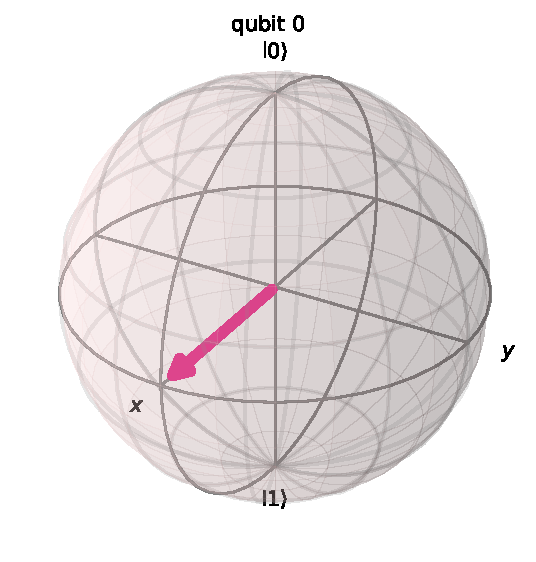
\includegraphics[keepaspectratio]{apostila_files/figure-pdf/cell-80-output-1.pdf}}

\begin{verbatim}
Estado após primeiro H: Statevector([0.70710678+0.j, 0.70710678+0.j],
            dims=(2,))
\end{verbatim}

\pandocbounded{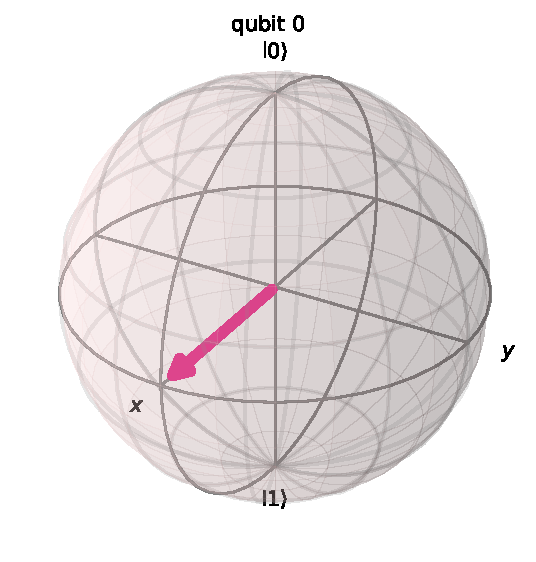
\includegraphics[keepaspectratio]{apostila_files/figure-pdf/cell-80-output-3.pdf}}

\begin{verbatim}
Estado após primeiro H: Statevector([0.70710678+0.j, 0.70710678+0.j],
            dims=(2,))
\end{verbatim}

\begin{Shaded}
\begin{Highlighting}[]
\CommentTok{\# Q{-}Sphere após o primeiro H}
\NormalTok{display(plot\_state\_qsphere(vetor\_apos\_h1))}
\end{Highlighting}
\end{Shaded}

\pandocbounded{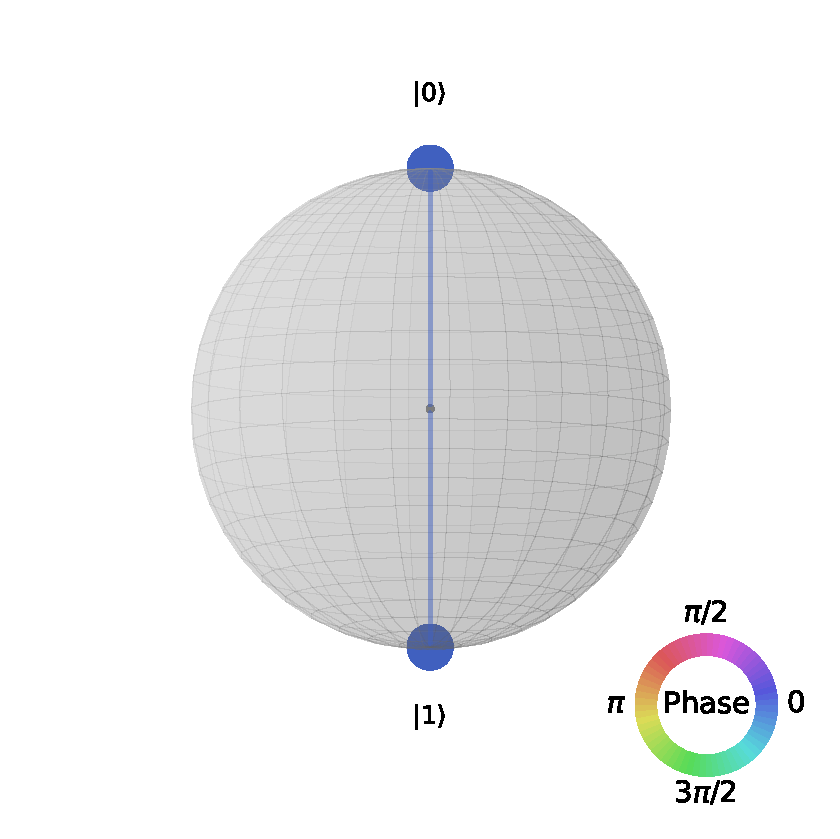
\includegraphics[keepaspectratio]{apostila_files/figure-pdf/cell-81-output-1.pdf}}

\pandocbounded{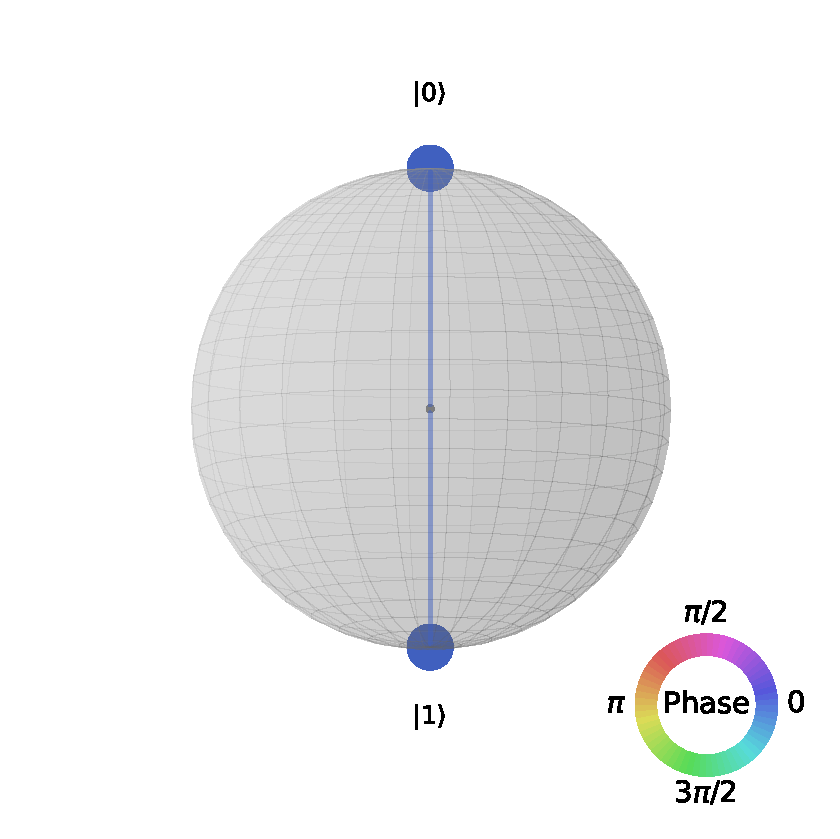
\includegraphics[keepaspectratio]{apostila_files/figure-pdf/cell-81-output-2.pdf}}

\begin{Shaded}
\begin{Highlighting}[]
\CommentTok{\# Passo 2: O fóton viaja pelos caminhos e encontra o SEGUNDO espelho}
\CommentTok{\# A interferência acontece aqui.}
\NormalTok{qc.h(}\DecValTok{0}\NormalTok{)}
\end{Highlighting}
\end{Shaded}

\begin{verbatim}
<qiskit.circuit.instructionset.InstructionSet at 0x7779e83d9150>
\end{verbatim}

\subsection{Visualização após o segundo Hadamard (Espelho
Semitransparente 2 -
Interferência)}\label{visualizauxe7uxe3o-apuxf3s-o-segundo-hadamard-espelho-semitransparente-2---interferuxeancia}

\begin{Shaded}
\begin{Highlighting}[]
\CommentTok{\# Esfera de Bloch após o segundo H}
\NormalTok{vetor\_apos\_h2 }\OperatorTok{=}\NormalTok{ Statevector(qc)}
\NormalTok{display(plot\_bloch\_multivector(vetor\_apos\_h2))}
\BuiltInTok{print}\NormalTok{(}\SpecialStringTok{f"Estado após segundo H: }\SpecialCharTok{\{}\NormalTok{vetor\_apos\_h2}\SpecialCharTok{\}}\SpecialStringTok{"}\NormalTok{)}
\end{Highlighting}
\end{Shaded}

\pandocbounded{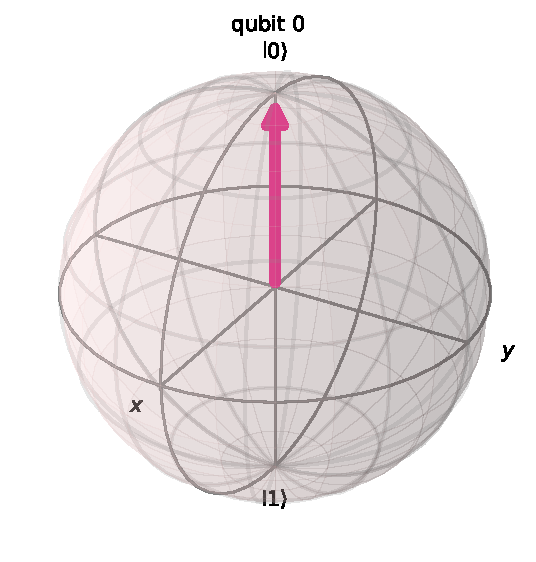
\includegraphics[keepaspectratio]{apostila_files/figure-pdf/cell-83-output-1.pdf}}

\begin{verbatim}
Estado após segundo H: Statevector([1.+0.j, 0.+0.j],
            dims=(2,))
\end{verbatim}

\pandocbounded{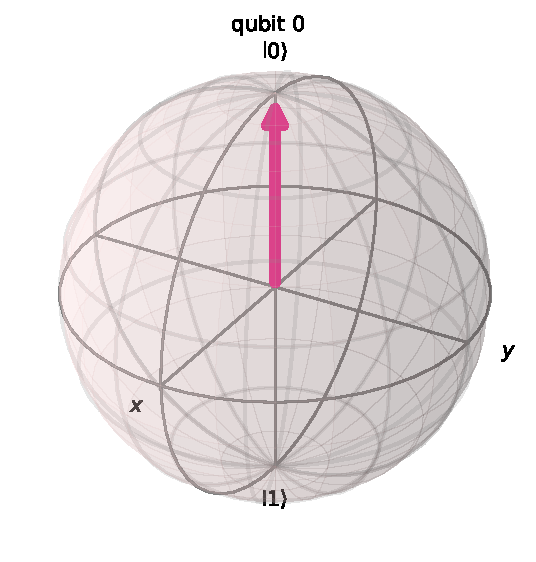
\includegraphics[keepaspectratio]{apostila_files/figure-pdf/cell-83-output-3.pdf}}

\begin{verbatim}
Estado após segundo H: Statevector([1.+0.j, 0.+0.j],
            dims=(2,))
\end{verbatim}

\begin{Shaded}
\begin{Highlighting}[]
\CommentTok{\# Q{-}Sphere após o segundo H}
\NormalTok{display(plot\_state\_qsphere(vetor\_apos\_h2))}
\end{Highlighting}
\end{Shaded}

\pandocbounded{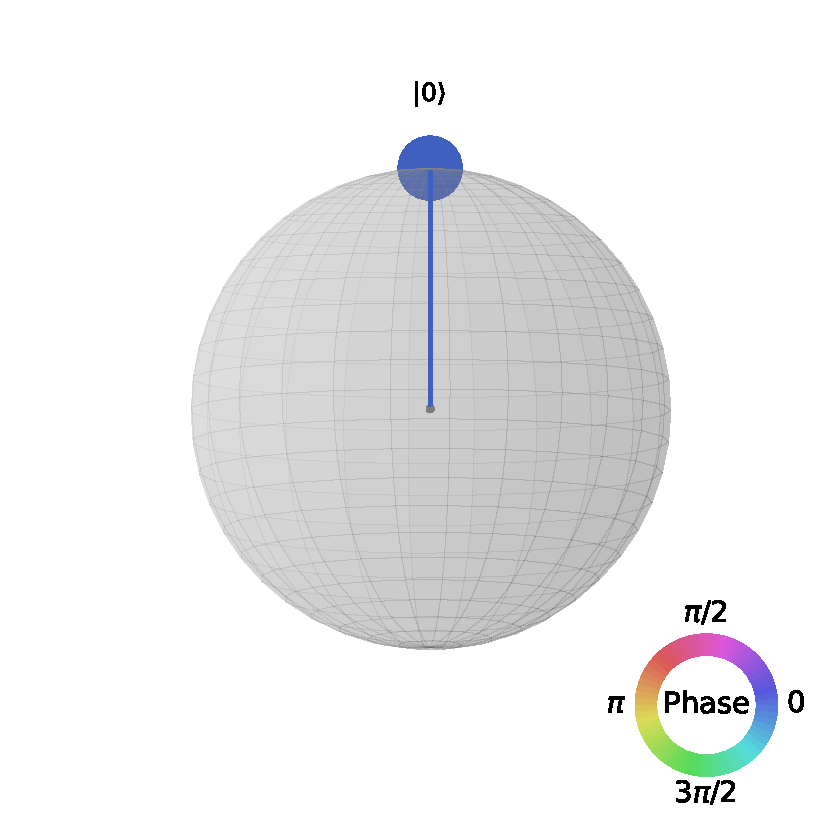
\includegraphics[keepaspectratio]{apostila_files/figure-pdf/cell-84-output-1.pdf}}

\pandocbounded{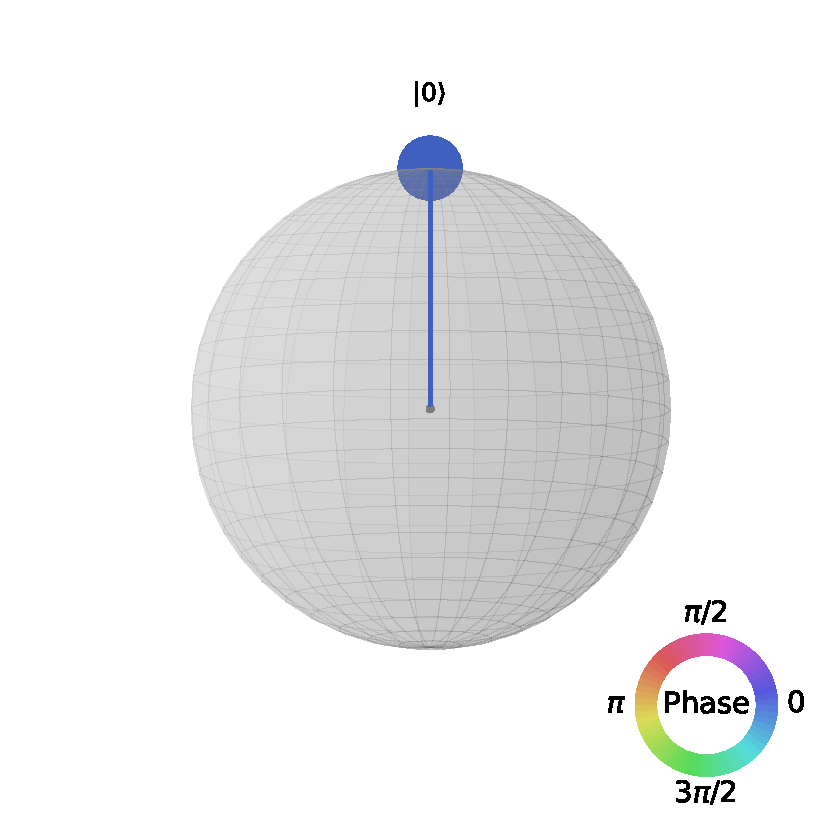
\includegraphics[keepaspectratio]{apostila_files/figure-pdf/cell-84-output-2.pdf}}

\subsection{Visualização do Circuito
Completo}\label{visualizauxe7uxe3o-do-circuito-completo}

\begin{Shaded}
\begin{Highlighting}[]
\CommentTok{\# Verificação}
\NormalTok{vetor }\OperatorTok{=}\NormalTok{ Statevector(qc)}
\BuiltInTok{print}\NormalTok{(vetor)}
\end{Highlighting}
\end{Shaded}

\begin{verbatim}
Statevector([1.+0.j, 0.+0.j],
            dims=(2,))
\end{verbatim}

\begin{verbatim}
Statevector([1.+0.j, 0.+0.j],
            dims=(2,))
\end{verbatim}

\begin{Shaded}
\begin{Highlighting}[]
\CommentTok{\# Desenho do circuito quântico}
\NormalTok{qc.draw(}\StringTok{\textquotesingle{}mpl\textquotesingle{}}\NormalTok{)}
\end{Highlighting}
\end{Shaded}

\pandocbounded{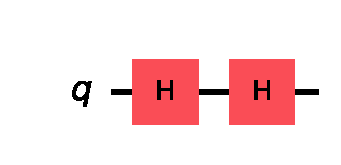
\includegraphics[keepaspectratio]{apostila_files/figure-pdf/cell-86-output-1.pdf}}

\pandocbounded{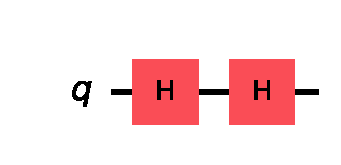
\includegraphics[keepaspectratio]{apostila_files/figure-pdf/cell-86-output-2.pdf}}

\chapter{Interpretação Física da Porta
Hadamard}\label{interpretauxe7uxe3o-fuxedsica-da-porta-hadamard}

\section{Mais Sobre a Porta Hadamard e sua Interpretação
Física}\label{mais-sobre-a-porta-hadamard-e-sua-interpretauxe7uxe3o-fuxedsica}

\textbf{Se um fóton ultrapassa uma espelho perfeitamente
semitransparente, qual o percentual de luz que transpassa o espelho e
qual o percentual de luz que é refletida?}

Essa pergunta é fundamental, pois ela é o elo entre o mundo físico e o
código que foi escrito em \url{01-intro.ipynb} (\texttt{qc.h(0)}) e em
\url{00-math.ipynb}.

A resposta depende se você está falando de \textbf{um raio de luz}
(mundo clássico) ou de \textbf{um único fóton} (mundo quântico).

\subsection{1. A Resposta Clássica (Um feixe de
luz)}\label{a-resposta-cluxe1ssica-um-feixe-de-luz}

Se você apontar um laser (que contém trilhões de fótons) para um espelho
perfeitamente semitransparente (conhecido tecnicamente como \textbf{Beam
Splitter} ou Divisor de Feixe 50/50):

\begin{itemize}
\tightlist
\item
  \textbf{50\%} da intensidade da luz atravessa.
\item
  \textbf{50\%} da intensidade da luz é refletida.
\end{itemize}

\subsection{2. A Resposta Quântica (Um único
fóton)}\label{a-resposta-quuxe2ntica-um-uxfanico-fuxf3ton}

Aqui a intuição quebra. Um fóton é uma partícula elementar, um
``pacote'' indivisível de energia. \textbf{Você não pode ter meio
fóton.} Ele não pode se partir ao meio como uma gota de água.

Então, o que acontece com \textbf{um} fóton?

\begin{itemize}
\tightlist
\item
  Ele entra em \textbf{Superposição}.
\item
  Ele é refletido \textbf{E} transmitido ao mesmo tempo.
\end{itemize}

\textbf{O Percentual:} A probabilidade dele ser detectado em um lado é
50\%, e no outro lado é 50\%. Mas, até que você coloque um detector
(faça uma medição), o fóton percorre \textbf{ambos os caminhos
simultaneamente}.

\subsection{A Conexão com o Código
Python}\label{a-conexuxe3o-com-o-cuxf3digo-python}

Lembra-se da porta Hadamard (\texttt{qc.h(0)}) e do fator
\(\frac{1}{\sqrt{2}}\)?

Fisicamente, a \textbf{Porta Hadamard É esse espelho semitransparente}.

Quando você escreve em Python:

\begin{Shaded}
\begin{Highlighting}[]
\NormalTok{qc.h(}\DecValTok{0}\NormalTok{)}
\end{Highlighting}
\end{Shaded}

Você está dizendo matematicamente:

\[|0\rangle \rightarrow \frac{|0\rangle + |1\rangle}{\sqrt{2}}\]

Isso é a descrição matemática exata de um fóton encontrando um espelho
50/50:

\begin{enumerate}
\def\labelenumi{\arabic{enumi}.}
\tightlist
\item
  O estado \(|0\rangle\) é o fóton chegando pelo caminho de cima.
\item
  Ao bater no espelho (H), ele se divide em dois caminhos possíveis.
\item
  O quadrado do coeficiente (\(\frac{1}{\sqrt{2}}\)) é \(\frac{1}{2}\),
  ou seja, \textbf{50\%}.
\end{enumerate}

\subsection{Por que isso importa para o próximo
passo?}\label{por-que-isso-importa-para-o-pruxf3ximo-passo}

Se você colocar \textbf{dois} espelhos desses em sequência, acontece a
\textbf{Interferência} (o assunto a estudar a seguir).

\begin{enumerate}
\def\labelenumi{\arabic{enumi}.}
\tightlist
\item
  O primeiro espelho separa os caminhos (cria superposição).
\item
  Os caminhos se cruzam novamente.
\item
  O segundo espelho recombina os caminhos.
\end{enumerate}

Se a matemática estiver certa, o fóton pode sair 100\% das vezes por uma
única saída, porque as ondas de probabilidade do caminho ``refletido''
se cancelam com as do caminho ``transmitido''.

Isso faz sentido? O espelho é o ``hardware'' que executa a função lógica
``Hadamard''.

\section{Isso foi feito esperimentalmente na vida
real?}\label{isso-foi-feito-esperimentalmente-na-vida-real}

Sim, e é um dos experimentos mais repetidos e comprovados da história da
física.

O experimento específico que demonstra o que discutimos (o fóton
passando por dois espelhos semitransparentes e interferindo consigo
mesmo) chama-se \textbf{Interferômetro de Mach-Zehnder}.

A realização desse experimento com \textbf{fótons individuais} (um de
cada vez) é o que prova que a mecânica quântica é real e não apenas uma
teoria matemática bonita.

Aqui está como isso acontece na vida real versus o que a nossa intuição
esperaria:

\subsection{1. O Experimento (O Interferômetro de
Mach-Zehnder)}\label{o-experimento-o-interferuxf4metro-de-mach-zehnder}

Imagine uma mesa de laboratório com a seguinte configuração:

\begin{figure}[H]

{\centering \pandocbounded{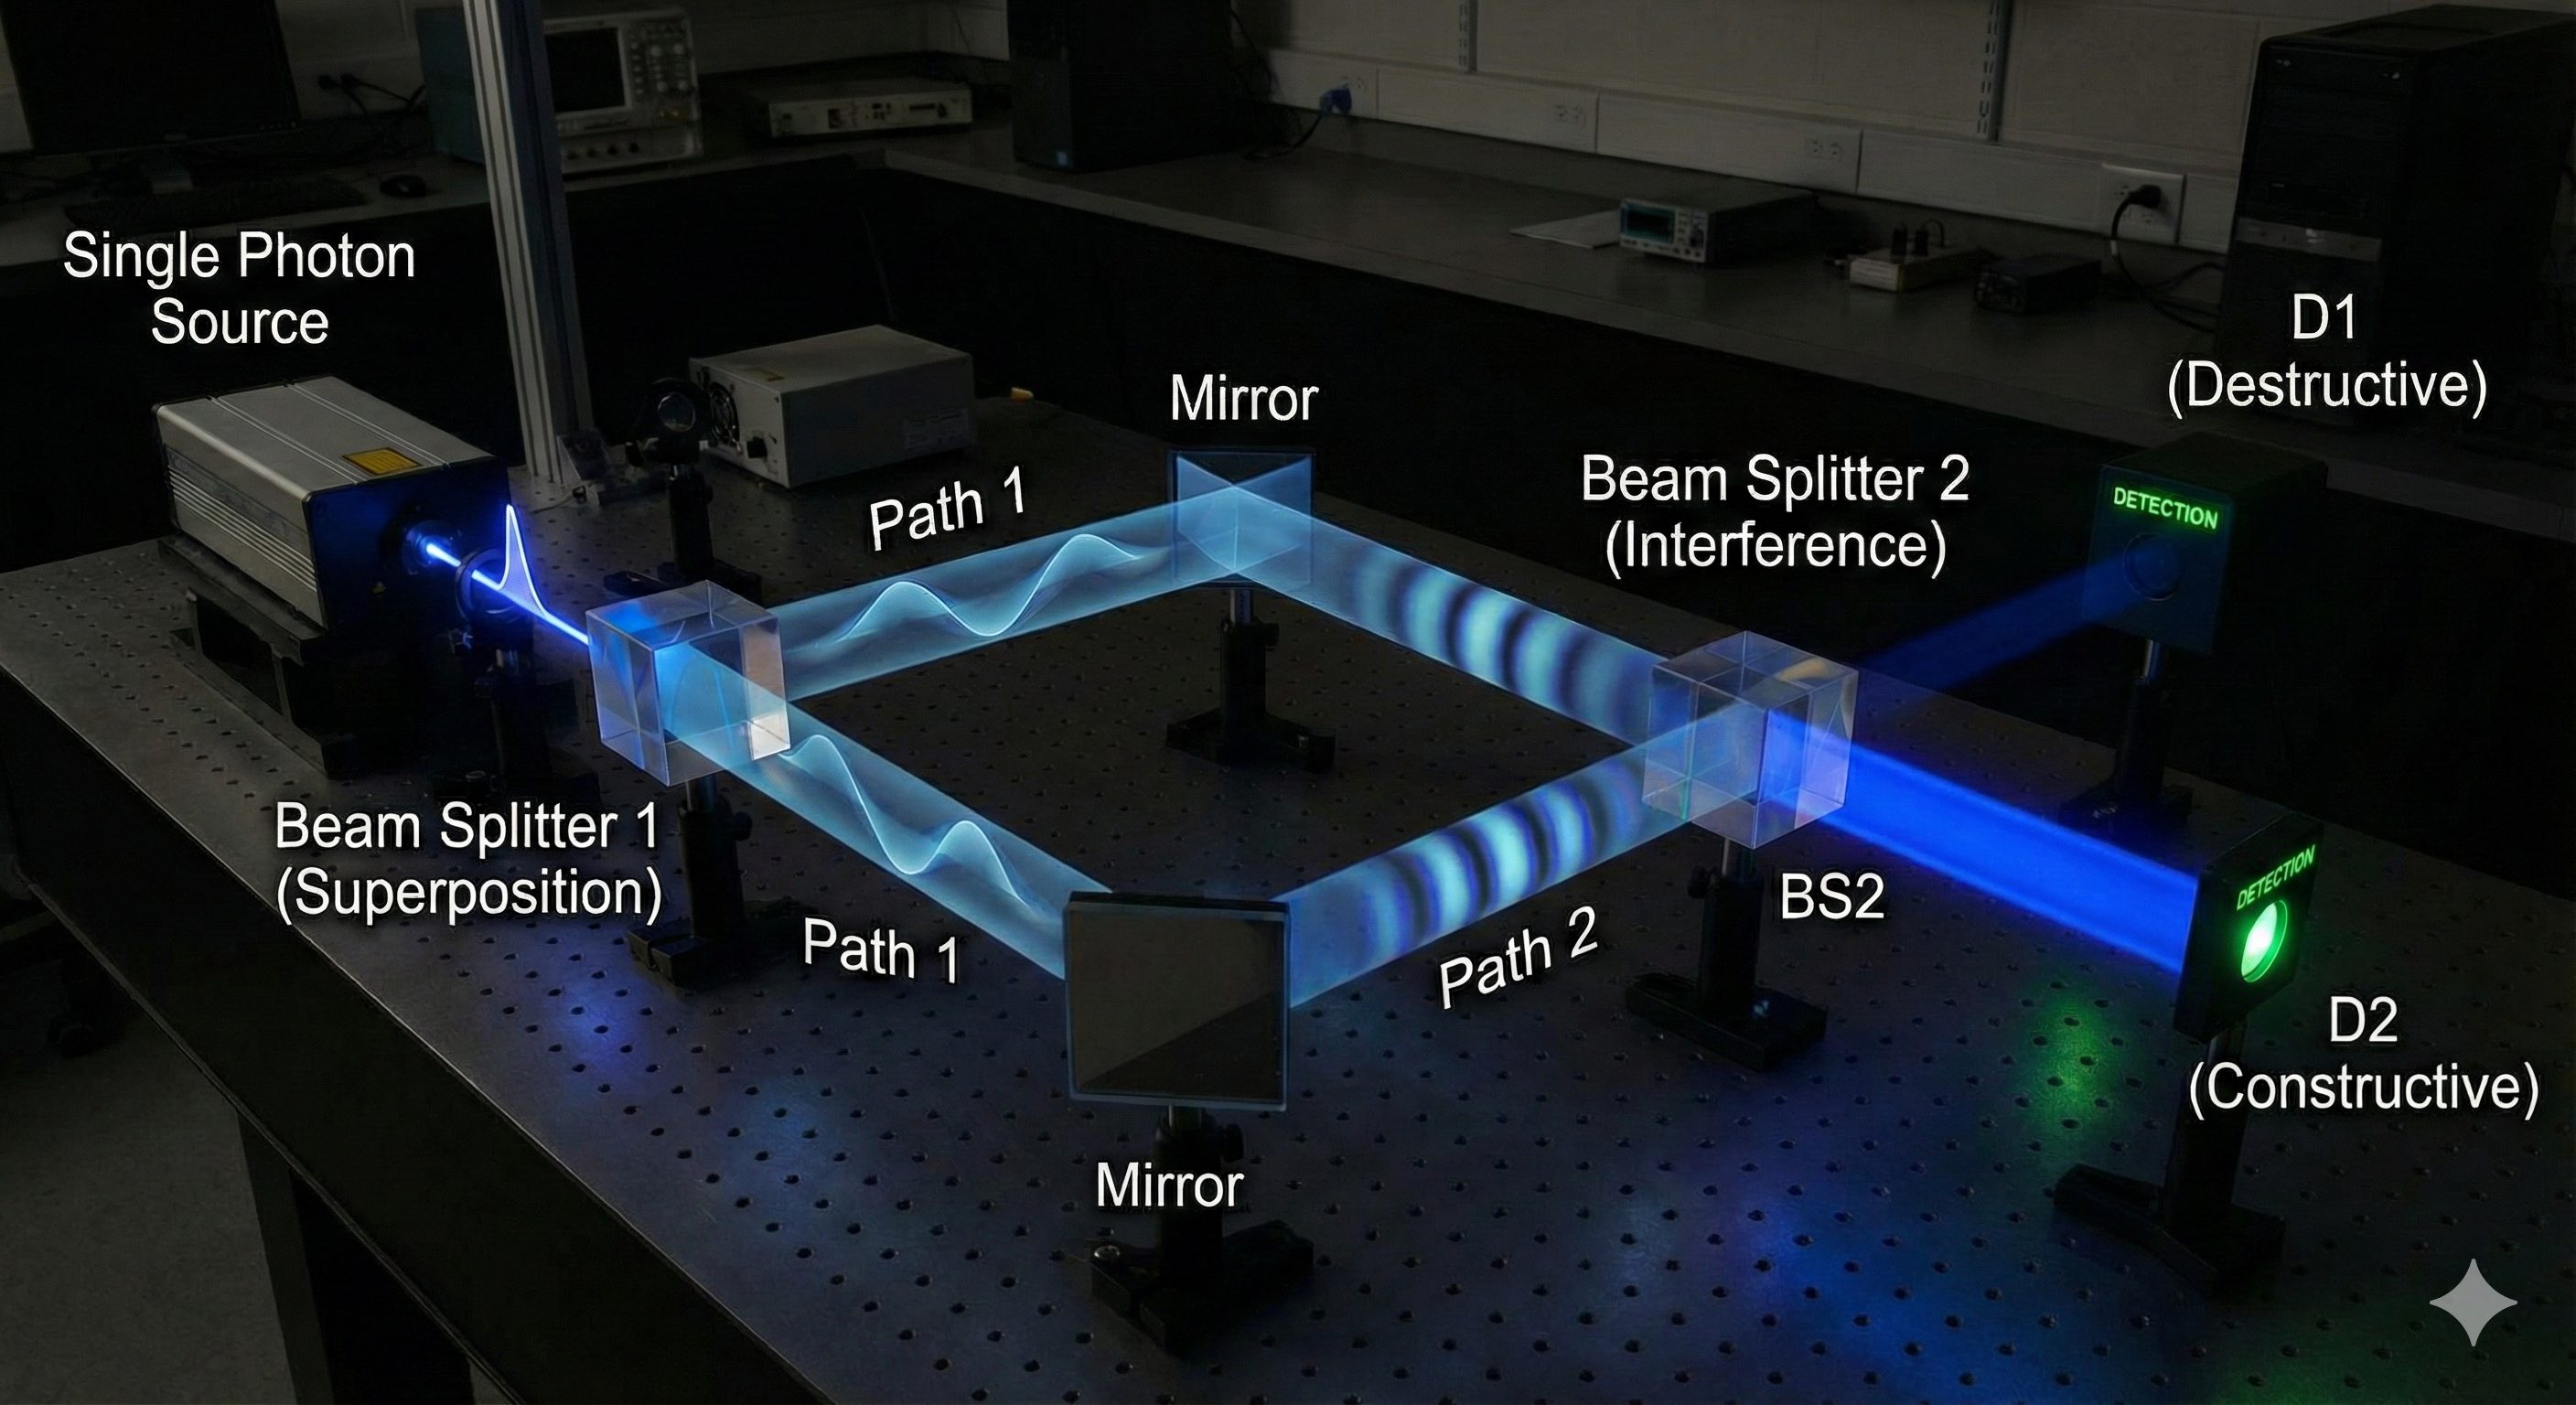
\includegraphics[keepaspectratio]{apostila_files/mediabag/interferometer.png}}

}

\caption{Interferômetro de Mach-Zehnder}

\end{figure}%

\begin{enumerate}
\def\labelenumi{\arabic{enumi}.}
\tightlist
\item
  \textbf{Fonte:} Dispara um \textbf{único fóton}.
\item
  \textbf{Espelho A ou \emph{Beam Splitter 1} (Hadamard 1):}
  Semitransparente. Divide o caminho.
\item
  \textbf{Caminhos:} O fóton pode ir pela direita ou esquerda.
\item
  \textbf{Espelho B ou \emph{Beam Splitter 2} (Hadamard 2):}
  Semitransparente. Reúne os caminhos antes dos detetores.
\item
  \textbf{Detetores D1 e D2:} Um no final de cada saída.
\end{enumerate}

\subsection{2. A Expectativa ``Clássica''
(Intuição)}\label{a-expectativa-cluxe1ssica-intuiuxe7uxe3o}

Se o fóton fosse uma bolinha física (como uma bola de gude):

\begin{enumerate}
\def\labelenumi{\arabic{enumi}.}
\tightlist
\item
  No primeiro espelho, ele escolheria aleatoriamente ir para a direita
  ou para a esquerda (50/50).
\item
  No segundo espelho, ele escolheria novamente aleatoriamente (50/50).
\item
  \textbf{Resultado esperado:} 50\% dos fótons chegariam ao Detetor 1 e
  50\% ao Detetor 2.
\end{enumerate}

\subsection{3. A Realidade ``Quântica'' (O que acontece no
laboratório)}\label{a-realidade-quuxe2ntica-o-que-acontece-no-laboratuxf3rio}

Quando fazemos isso na vida real, com espelhos perfeitamente alinhados:

\begin{itemize}
\tightlist
\item
  \textbf{100\%} dos fótons chegam ao \textbf{Detetor 1}.
\item
  \textbf{0\%} dos fótons chegam ao \textbf{Detetor 2}.
\end{itemize}

\textbf{Por que?} Interferência. O fóton ``passou'' pelos dois caminhos
ao mesmo tempo. As ondas de probabilidade que foram para o Detetor 2
chegaram com fases opostas (como uma onda do mar subindo encontrando uma
descendo) e se cancelaram (\textbf{Interferência Destrutiva}). As ondas
que foram para o Detetor 1 se somaram.

\subsubsection{Demonstração do Interferômetro de
Mach-Zehnder}\label{demonstrauxe7uxe3o-do-interferuxf4metro-de-mach-zehnder}

\begin{figure}[H]

{\centering \pandocbounded{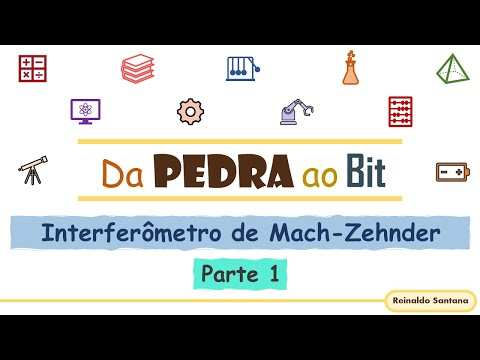
\includegraphics[keepaspectratio]{apostila_files/mediabag/0.jpg}}

}

\caption{Assistir demonstração no YouTube}

\end{figure}%

\textbf{\href{https://www.youtube.com/watch?v=M3Y2hwsJgos}{▶️ Clique
aqui para assistir a demonstração do Interferômetro de Mach-Zehnder}}

Este vídeo é relevante porque exibe a montagem óptica real do
experimento discutido, permitindo visualizar os espelhos e o padrão de
luz resultante que comprova o fenômeno da interferência.

\subsection{4. Como isso se traduz no código
Python?}\label{como-isso-se-traduz-no-cuxf3digo-python}

Você pode replicar esse experimento físico agora mesmo no Qiskit. É a
prova de que a porta Hadamard é reversível.

Matematicamente, aplicar dois Hadamards é igual a não fazer nada
(Identidade), pois as superposições se cancelam e voltam ao estado
original.

\begin{Shaded}
\begin{Highlighting}[]
\ImportTok{from}\NormalTok{ qiskit }\ImportTok{import}\NormalTok{ QuantumCircuit}
\ImportTok{from}\NormalTok{ qiskit.quantum\_info }\ImportTok{import}\NormalTok{ Statevector}

\NormalTok{qc }\OperatorTok{=}\NormalTok{ QuantumCircuit(}\DecValTok{1}\NormalTok{)}

\CommentTok{\# Passo 1: O fóton encontra o primeiro espelho}
\CommentTok{\# Estado: Superposição (50/50)}
\NormalTok{qc.h(}\DecValTok{0}\NormalTok{) }

\CommentTok{\# Passo 2: O fóton viaja pelos caminhos e encontra o SEGUNDO espelho}
\CommentTok{\# A interferência acontece aqui.}
\NormalTok{qc.h(}\DecValTok{0}\NormalTok{)}

\CommentTok{\# Verificação}
\NormalTok{vetor }\OperatorTok{=}\NormalTok{ Statevector(qc)}
\BuiltInTok{print}\NormalTok{(vetor)}
\end{Highlighting}
\end{Shaded}

\textbf{Resultado:} Você verá que o vetor volta a ser
\texttt{{[}1,\ 0{]}} (Estado puro). O computador quântico simulou a
interferência destrutiva que ocorreria no laboratório.

\begin{quote}
Veja código completo em \href{04-Hadamard-experiment.ipynb}{Código
04-Hadamard-experiment.ipynb}
\end{quote}

\subsection{Curiosidade Histórica: O Prêmio Nobel de
2022}\label{curiosidade-histuxf3rica-o-pruxeamio-nobel-de-2022}

A confirmação experimental de que isso acontece com partículas
individuais e que o emaranhamento é real (violando a intuição clássica)
foi tão importante que o \textbf{Prêmio Nobel de Física de 2022} foi
dado a Alain Aspect, John Clauser e Anton Zeilinger.

Eles provaram, sem sombra de dúvidas, que a natureza se comporta dessa
maneira estranha. Não é uma falha de medição; é a arquitetura
fundamental do universo.

\newpage

\chapter{Módulo 9: Interferência e
Deutsch-Jozsa}\label{muxf3dulo-9-interferuxeancia-e-deutsch-jozsa}

\chapter{Aula 09 --- Interferência Quântica e Algoritmo de
Deutsch-Jozsa}\label{aula-09-interferuxeancia-quuxe2ntica-e-algoritmo-de-deutsch-jozsa}

\chapter{Interferência Quântica e
Algoritmos}\label{interferuxeancia-quuxe2ntica-e-algoritmos}

\section{📖 Visão Geral}\label{visuxe3o-geral}

Bem-vindo ao notebook mais avançado desta série! Aqui vamos mergulhar
nos mecanismos que tornam os \textbf{algoritmos quânticos}
fundamentalmente diferentes (e mais poderosos) que os clássicos.

\subsection{🎯 O Que Você Vai
Aprender}\label{o-que-vocuxea-vai-aprender-1}

\begin{enumerate}
\def\labelenumi{\arabic{enumi}.}
\tightlist
\item
  \textbf{Phase Kickback (Coice de Fase)}

  \begin{itemize}
  \tightlist
  \item
    O mecanismo ``secreto'' dos algoritmos quânticos
  \item
    Como o qubit alvo pode afetar o qubit de controle
  \item
    Demonstração prática com visualizações
  \end{itemize}
\item
  \textbf{Algoritmo de Deutsch-Jozsa}

  \begin{itemize}
  \tightlist
  \item
    Primeiro algoritmo a demonstrar vantagem quântica
  \item
    Resolve um problema com UMA consulta (vs.~exponencialmente muitas)
  \item
    Implementação completa do zero
  \end{itemize}
\end{enumerate}

\subsection{📚 Pré-requisitos}\label{pruxe9-requisitos}

Antes de continuar, certifique-se de que você entende:

\begin{itemize}
\tightlist
\item
  ✅ \textbf{Superposição} - de \url{01-intro.ipynb}
\item
  ✅ \textbf{Emaranhamento} - de \url{02-teletransport.ipynb}
\item
  ✅ \textbf{Porta Hadamard} - de \url{04-Hadamard-experiment.ipynb}
\item
  ✅ \textbf{Interferência básica} - H × H = I
\end{itemize}

\subsection{🎓 Nível de Dificuldade}\label{nuxedvel-de-dificuldade}

\textbf{Intermediário a Avançado} - Este notebook assume familiaridade
com: - Notação de Dirac (\(|0\rangle, |1\rangle, |+\rangle, |-\rangle\))
- Portas quânticas básicas (H, X, CNOT) - Conceito de fase em estados
quânticos - Produto tensorial (\(\otimes\))

\subsection{💡 Por Que Este Conteúdo é
Importante?}\label{por-que-este-conteuxfado-uxe9-importante}

\textbf{Phase Kickback} é o ``ingrediente secreto'' que faz algoritmos
como: - 🔍 \textbf{Grover} (busca quântica) - quadraticamente mais
rápido - 🔢 \textbf{Shor} (fatoração) - exponencialmente mais rápido
(quebra RSA!) - ⚗️ \textbf{QPE} (estimação de fase) - base da química
quântica

Sem entender kickback, algoritmos quânticos parecem ``mágica''. Com esse
entendimento, você verá a lógica elegante por trás da supremacia
quântica.

\subsection{🗺️ Estrutura do Notebook}\label{estrutura-do-notebook}

\begin{Shaded}
\begin{Highlighting}[]
\NormalTok{1. Phase Kickback}
\NormalTok{   ├── Conceito e Analogia}
\NormalTok{   ├── Matemática Detalhada}
\NormalTok{   ├── Demonstração Prática}
\NormalTok{   └── Visualizações (Bloch + Q{-}Sphere)}

\NormalTok{2. Deutsch{-}Jozsa}
\NormalTok{   ├── Definição do Problema}
\NormalTok{   ├── Oráculos (Constante vs. Balanceado)}
\NormalTok{   ├── Implementação Completa}
\NormalTok{   └── Análise de Resultados}

\NormalTok{3. Resumo e Próximos Passos}
\NormalTok{   └── Conexões com Algoritmos Avançados}
\end{Highlighting}
\end{Shaded}

\textbf{Dica:} Execute as células em ordem sequencial. Cada visualização
ajuda a construir a intuição para o próximo conceito!

\section{Phase Kickback e o Algoritmo de
Deutsch-Jozsa}\label{phase-kickback-e-o-algoritmo-de-deutsch-jozsa}

Vamos mergulhar no mecanismo que faz os algoritmos quânticos
funcionarem.

Até agora, a intuição foi: ``O qubit de controle manda no qubit alvo''.

Lembra da porta CNOT em \url{01-intro.ipynb}?

No \textbf{Phase Kickback} (Coice de Fase), descobrimos que a relação é
uma via de mão dupla. O qubit alvo pode alterar o estado do qubit de
controle.

É aqui que a ``mágica'' acontece.

\subsection{1. O Conceito: Phase Kickback (O Recuo da
Arma)}\label{o-conceito-phase-kickback-o-recuo-da-arma}

Imagine que você está disparando uma arma de fogo:

\begin{enumerate}
\def\labelenumi{\arabic{enumi}.}
\tightlist
\item
  \textbf{Ação:} Você (Controle) aperta o gatilho.
\item
  \textbf{Efeito:} A bala (Alvo) sai.
\item
  \textbf{Reação:} O seu ombro sente um ``coice'' ou recuo para trás.
\end{enumerate}

Na computação quântica, se prepararmos o qubit alvo de uma maneira
específica, a operação ``bate'' nele e volta, alterando a fase do
controle.

\subsubsection{A Matemática
(Simplificada)}\label{a-matemuxe1tica-simplificada}

Vamos usar a porta CNOT.

\begin{itemize}
\tightlist
\item
  Alvo Normal (\(|0\rangle\) ou \(|1\rangle\)): O CNOT inverte o valor
  (0 vira 1).
\item
  Alvo em Autestado (\(|-\rangle\)): O estado \(|-\rangle\) (que é
  \(H|1\rangle\)) é especial para a porta X (NOT).
\end{itemize}

\[X|-\rangle = -|-\rangle\]

(A porta X apenas adiciona um sinal negativo, uma fase de 180º).

\paragraph{\texorpdfstring{Mais sobre o estado
\(|-\rangle\)}{Mais sobre o estado \textbar-\textbackslash rangle}}\label{mais-sobre-o-estado--rangle}

O estado \(|-\rangle\) é um dos \textbf{estados de superposição
fundamentais} em computação quântica. Vou explicar:

\textbf{O que é \(|-\rangle\)?}

\[|-\rangle = \frac{|0\rangle - |1\rangle}{\sqrt{2}}\]

É uma \textbf{superposição} de \(|0\rangle\) e \(|1\rangle\) com uma
diferença de fase de 180° entre eles (note o sinal \textbf{negativo}).

\textbf{Por que \(|-\rangle = H|1\rangle\)?}

Aplicando a porta Hadamard (H) ao estado \(|1\rangle\):

\[H|1\rangle = H \begin{pmatrix} 0 \\ 1 \end{pmatrix} = \frac{1}{\sqrt{2}} \begin{pmatrix} 1 & 1 \\ 1 & -1 \end{pmatrix} \begin{pmatrix} 0 \\ 1 \end{pmatrix}\]

\[= \frac{1}{\sqrt{2}} \begin{pmatrix} 1 \\ -1 \end{pmatrix} = \frac{|0\rangle - |1\rangle}{\sqrt{2}} = |-\rangle\]

\paragraph{\texorpdfstring{Comparação com
\(|+\rangle\)}{Comparação com \textbar+\textbackslash rangle}}\label{comparauxe7uxe3o-com-rangle}

\begin{itemize}
\tightlist
\item
  \(|+\rangle = H|0\rangle = \frac{|0\rangle + |1\rangle}{\sqrt{2}}\)
  (sinal \textbf{positivo})
\item
  \(|-\rangle = H|1\rangle = \frac{|0\rangle - |1\rangle}{\sqrt{2}}\)
  (sinal \textbf{negativo})
\end{itemize}

\paragraph{\texorpdfstring{Por que \(|-\rangle\) é especial para o Phase
Kickback?}{Por que \textbar-\textbackslash rangle é especial para o Phase Kickback?}}\label{por-que--rangle-uxe9-especial-para-o-phase-kickback}

O estado \(|-\rangle\) é um \textbf{autoestado} da porta X (NOT):

\[X|-\rangle = -|-\rangle\]

A porta X apenas adiciona uma fase global negativa, mas não muda o
estado. Essa propriedade permite que a fase ``retorne'' para o qubit de
controle no CNOT, criando o efeito de \textbf{Phase Kickback}.

Quando aplicamos CNOT com o alvo em \(|-\rangle\):

\begin{itemize}
\tightlist
\item
  Se o controle for \(|0\rangle\), nada acontece.
\item
  Se o controle for \(|1\rangle\), o alvo ganha um sinal de menos
  (\(-\)).
\item
  Como o alvo não mudou visualmente (continua \(|-\rangle\)), esse sinal
  de menos migra para o qubit de controle.
\end{itemize}

Resultado: O controle, que era \(|+\rangle\), vira \(|-\rangle\). O alvo
não muda.

\subsubsection{Código completo do Phase
Kickback}\label{cuxf3digo-completo-do-phase-kickback}

Segue o código completo para demonstrar o Phase Kickback usando Qiskit.
Logo após, faremos uma análise detalhada de cada etapa.

\begin{Shaded}
\begin{Highlighting}[]
\ImportTok{from}\NormalTok{ qiskit }\ImportTok{import}\NormalTok{ QuantumCircuit, transpile}
\ImportTok{from}\NormalTok{ qiskit\_aer }\ImportTok{import}\NormalTok{ AerSimulator}
\ImportTok{from}\NormalTok{ qiskit.quantum\_info }\ImportTok{import}\NormalTok{ Statevector}
\ImportTok{from}\NormalTok{ qiskit.visualization }\ImportTok{import}\NormalTok{ plot\_bloch\_multivector, plot\_state\_qsphere}
\end{Highlighting}
\end{Shaded}

\begin{Shaded}
\begin{Highlighting}[]
\CommentTok{\# Criar circuito com 2 qubits}
\NormalTok{qc }\OperatorTok{=}\NormalTok{ QuantumCircuit(}\DecValTok{2}\NormalTok{, }\DecValTok{1}\NormalTok{)  }\CommentTok{\# 2 Qubits, 1 Bit clássico}
\NormalTok{qc.draw(}\StringTok{"mpl"}\NormalTok{)}

\CommentTok{\# 1. PREPARAÇÃO}
\CommentTok{\# Colocar o Qubit 0 (Controle) em Superposição |+\textgreater{}}
\NormalTok{qc.h(}\DecValTok{0}\NormalTok{)}

\CommentTok{\# Colocar o Qubit 1 (Alvo) no estado |{-} \textgreater{}}
\CommentTok{\# Para isso: aplicamos X (vira 1) e depois H (vira menos)}
\NormalTok{qc.x(}\DecValTok{1}\NormalTok{)}
\NormalTok{qc.h(}\DecValTok{1}\NormalTok{)}

\CommentTok{\# 2. O KICKBACK}
\CommentTok{\# Aplicamos CNOT. O alvo (q1) está em |{-}\textgreater{}.}
\CommentTok{\# Isso deve fazer o q0 virar |{-}\textgreater{} "por tabela".}
\NormalTok{qc.cx(}\DecValTok{0}\NormalTok{, }\DecValTok{1}\NormalTok{)}

\CommentTok{\# 3. VERIFICAÇÃO}
\CommentTok{\# Como saber se q0 virou |{-}\textgreater{}?}
\CommentTok{\# Se aplicarmos H novamente:}
\CommentTok{\# H em |+\textgreater{} volta para 0}
\CommentTok{\# H em |{-}\textgreater{} volta para 1}
\NormalTok{qc.h(}\DecValTok{0}\NormalTok{)}

\CommentTok{\# Medimos APENAS o qubit de controle (q0)}
\NormalTok{qc.measure(}\DecValTok{0}\NormalTok{, }\DecValTok{0}\NormalTok{)}

\CommentTok{\# Executar}
\NormalTok{simulador }\OperatorTok{=}\NormalTok{ AerSimulator()}
\NormalTok{job }\OperatorTok{=}\NormalTok{ simulador.run(transpile(qc, simulador), shots}\OperatorTok{=}\DecValTok{1000}\NormalTok{)}
\BuiltInTok{print}\NormalTok{(}\StringTok{"Resultado do Controle:"}\NormalTok{, job.result().get\_counts())}
\end{Highlighting}
\end{Shaded}

\begin{verbatim}
Resultado do Controle: {'1': 1000}
\end{verbatim}

\pandocbounded{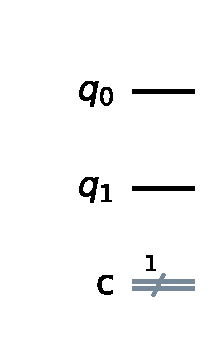
\includegraphics[keepaspectratio]{apostila_files/figure-pdf/cell-88-output-2.pdf}}

\begin{verbatim}
Resultado do Controle: {'1': 1000}
\end{verbatim}

\begin{Shaded}
\begin{Highlighting}[]
\CommentTok{\# Visualizar o circuito completo}
\NormalTok{qc.draw(}\StringTok{\textquotesingle{}mpl\textquotesingle{}}\NormalTok{)}
\end{Highlighting}
\end{Shaded}

\pandocbounded{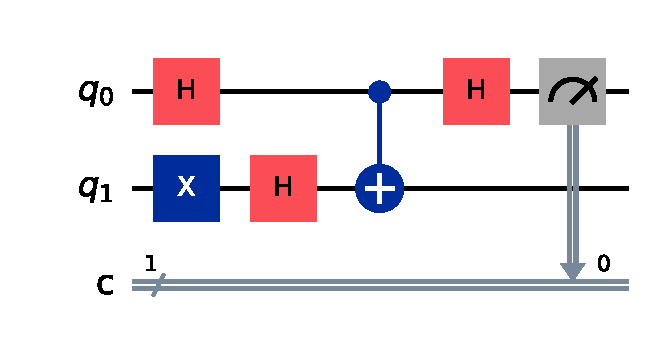
\includegraphics[keepaspectratio]{apostila_files/figure-pdf/cell-89-output-1.pdf}}

\pandocbounded{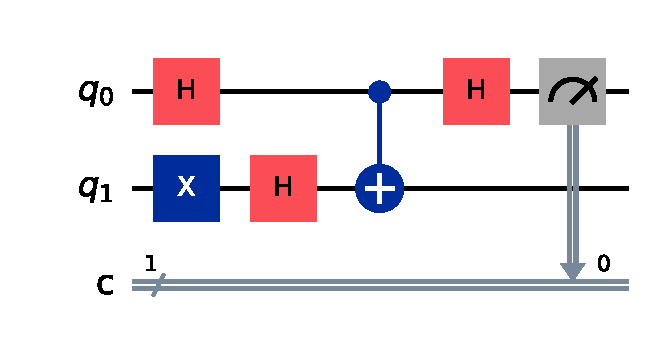
\includegraphics[keepaspectratio]{apostila_files/figure-pdf/cell-89-output-2.pdf}}

\subsubsection{Demonstração detalhada de Phase
Kickback}\label{demonstrauxe7uxe3o-detalhada-de-phase-kickback}

Vamos provar que o qubit de controle muda sem que nenhuma porta toque
nele diretamente.

\begin{Shaded}
\begin{Highlighting}[]
\CommentTok{\# Criar circuito com 2 qubits}
\NormalTok{qc }\OperatorTok{=}\NormalTok{ QuantumCircuit(}\DecValTok{2}\NormalTok{, }\DecValTok{1}\NormalTok{) }\CommentTok{\# 2 Qubits, 1 Bit clássico}

\CommentTok{\# Desenhar o circuito}
\NormalTok{qc.draw(}\StringTok{\textquotesingle{}mpl\textquotesingle{}}\NormalTok{)}
\end{Highlighting}
\end{Shaded}

\pandocbounded{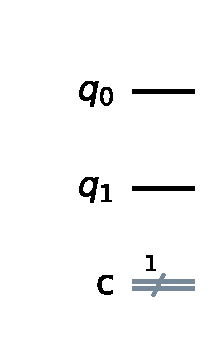
\includegraphics[keepaspectratio]{apostila_files/figure-pdf/cell-90-output-1.pdf}}

\pandocbounded{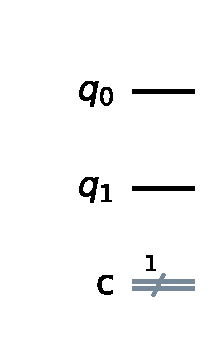
\includegraphics[keepaspectratio]{apostila_files/figure-pdf/cell-90-output-2.pdf}}

Matematicamente, os estados dos qubits, quando criados, são:

\begin{itemize}
\tightlist
\item
  Qubit 0 (Controle): \(|0\rangle\)
\item
  Qubit 1 (Alvo): \(|0\rangle\)
\end{itemize}

Estes estados iniciais representam \(|00\rangle\) do registrador
quântico.

\subsection{O Estado Inicial}\label{o-estado-inicial}

\begin{Shaded}
\begin{Highlighting}[]
\CommentTok{\# 1. PREPARAÇÃO}
\CommentTok{\# Colocar o Qubit 0 (Controle) em Superposição |+\textgreater{}}
\NormalTok{qc.h(}\DecValTok{0}\NormalTok{)}

\CommentTok{\# Colocar o Qubit 1 (Alvo) no estado |{-} \textgreater{} }
\CommentTok{\# Para isso: aplicamos X (vira 1) e depois H (vira menos)}
\NormalTok{qc.x(}\DecValTok{1}\NormalTok{)}
\NormalTok{qc.h(}\DecValTok{1}\NormalTok{)}

\CommentTok{\# Desenhar o circuito}
\NormalTok{qc.draw(}\StringTok{\textquotesingle{}mpl\textquotesingle{}}\NormalTok{)}
\end{Highlighting}
\end{Shaded}

\pandocbounded{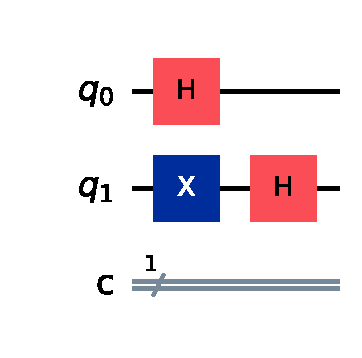
\includegraphics[keepaspectratio]{apostila_files/figure-pdf/cell-91-output-1.pdf}}

\pandocbounded{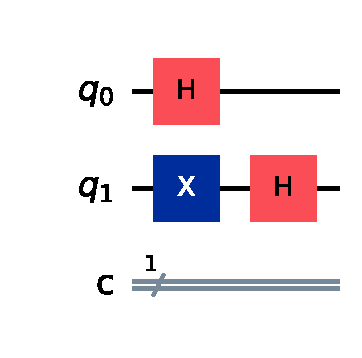
\includegraphics[keepaspectratio]{apostila_files/figure-pdf/cell-91-output-2.pdf}}

\subsubsection{Demonstração Matemática: Preparação do Estado
Inicial}\label{demonstrauxe7uxe3o-matemuxe1tica-preparauxe7uxe3o-do-estado-inicial}

O estado inicial preparado após a aplicação das portas Hadamard é:

\[|\psi_0\rangle = |+\rangle \otimes |-\rangle\]

Expandindo cada componente:

\[|+\rangle = \frac{|0\rangle + |1\rangle}{\sqrt{2}}\]

\[|-\rangle = \frac{|0\rangle - |1\rangle}{\sqrt{2}}\]

Portanto, o estado completo é:

\[|\psi_0\rangle = \frac{1}{\sqrt{2}}(|0\rangle + |1\rangle) \otimes \frac{1}{\sqrt{2}}(|0\rangle - |1\rangle)\]

Usando a representação matricial dos estados:

\[|0\rangle = \begin{pmatrix} 1 \\ 0 \end{pmatrix}, \quad |1\rangle = \begin{pmatrix} 0 \\ 1 \end{pmatrix}\]

\[|+\rangle = \frac{1}{\sqrt{2}}\begin{pmatrix} 1 \\ 1 \end{pmatrix}, \quad |-\rangle = \frac{1}{\sqrt{2}}\begin{pmatrix} 1 \\ -1 \end{pmatrix}\]

O produto tensorial \(|\psi_0\rangle = |+\rangle \otimes |-\rangle\) é
calculado como:
\[|\psi_0\rangle = \frac{1}{\sqrt{2}}\begin{pmatrix} 1 \\ 1 \end{pmatrix} \otimes \frac{1}{\sqrt{2}}\begin{pmatrix} 1 \\ -1 \end{pmatrix}\]

Primeiro, combinamos os coeficientes escalares:

\[= \frac{1}{\sqrt{2}} \cdot \frac{1}{\sqrt{2}} \begin{pmatrix} 1 \\ 1 \end{pmatrix} \otimes \begin{pmatrix} 1 \\ -1 \end{pmatrix} = \frac{1}{2}\begin{pmatrix} 1 \\ 1 \end{pmatrix} \otimes \begin{pmatrix} 1 \\ -1 \end{pmatrix}\]

Agora aplicamos a definição do produto tensorial (produto de Kronecker).
Para dois vetores
\(\mathbf{u} = \begin{pmatrix} u_1 \\ u_2 \end{pmatrix}\) e
\(\mathbf{v} = \begin{pmatrix} v_1 \\ v_2 \end{pmatrix}\):

\[\mathbf{u} \otimes \mathbf{v} = \begin{pmatrix} u_1 \mathbf{v} \\ u_2 \mathbf{v} \end{pmatrix} = \begin{pmatrix} u_1 v_1 \\ u_1 v_2 \\ u_2 v_1 \\ u_2 v_2 \end{pmatrix}\]

Aplicando ao nosso caso onde \(u_1 = 1\), \(u_2 = 1\), \(v_1 = 1\),
\(v_2 = -1\):

\[\begin{pmatrix} 1 \\ 1 \end{pmatrix} \otimes \begin{pmatrix} 1 \\ -1 \end{pmatrix} = \begin{pmatrix} 1 \cdot \begin{pmatrix} 1 \\ -1 \end{pmatrix} \\ 1 \cdot \begin{pmatrix} 1 \\ -1 \end{pmatrix} \end{pmatrix} = \begin{pmatrix} 1 \cdot 1 \\ 1 \cdot (-1) \\ 1 \cdot 1 \\ 1 \cdot (-1) \end{pmatrix} = \begin{pmatrix} 1 \\ -1 \\ 1 \\ -1 \end{pmatrix}\]

Multiplicando pelo coeficiente \(\frac{1}{2}\):
\[|\psi_0\rangle = \frac{1}{2}\begin{pmatrix} 1 \\ 1 \end{pmatrix} \otimes \begin{pmatrix} 1 \\ -1 \end{pmatrix}\]

Se você ainda não entendeu, vamos calcular o produto tensorial passo a
passo. O produto tensorial de dois vetores coluna funciona da seguinte
forma:

\textbf{Passo 1:} Pegue o primeiro elemento do primeiro vetor (que é
\(1\)) e multiplique-o por todo o segundo vetor:

\[1 \cdot \begin{pmatrix} 1 \\ -1 \end{pmatrix} = \begin{pmatrix} 1 \cdot 1 \\ 1 \cdot (-1) \end{pmatrix} = \begin{pmatrix} 1 \\ -1 \end{pmatrix}\]

\textbf{Passo 2:} Pegue o segundo elemento do primeiro vetor (que também
é \(1\)) e multiplique-o por todo o segundo vetor:

\[1 \cdot \begin{pmatrix} 1 \\ -1 \end{pmatrix} = \begin{pmatrix} 1 \cdot 1 \\ 1 \cdot (-1) \end{pmatrix} = \begin{pmatrix} 1 \\ -1 \end{pmatrix}\]

\textbf{Passo 3:} Empilhe os resultados verticalmente para formar um
vetor de 4 elementos:

\[\begin{pmatrix} 1 \\ 1 \end{pmatrix} \otimes \begin{pmatrix} 1 \\ -1 \end{pmatrix} = \begin{pmatrix} \text{resultado do passo 1} \\ \text{resultado do passo 2} \end{pmatrix} = \begin{pmatrix} 1 \\ -1 \\ 1 \\ -1 \end{pmatrix}\]

\textbf{Passo 4:} Multiplique o resultado pelo coeficiente
\(\frac{1}{2}\):

\[|\psi_0\rangle = \frac{1}{2}\begin{pmatrix} 1 \\ -1 \\ 1 \\ -1 \end{pmatrix} = \begin{pmatrix} \frac{1}{2} \cdot 1 \\ \frac{1}{2} \cdot (-1) \\ \frac{1}{2} \cdot 1 \\ \frac{1}{2} \cdot (-1) \end{pmatrix} = \begin{pmatrix} \frac{1}{2} \\ -\frac{1}{2} \\ \frac{1}{2} \\ -\frac{1}{2} \end{pmatrix}\]

Lembre-se que se expandirmos em termos da base computacional
\(\{|00\rangle, |01\rangle, |10\rangle, |11\rangle\}\):

\[|00\rangle = \begin{pmatrix} 1 \\ 0 \\ 0 \\ 0 \end{pmatrix}, \quad |01\rangle = \begin{pmatrix} 0 \\ 1 \\ 0 \\ 0 \end{pmatrix}, \quad |10\rangle = \begin{pmatrix} 0 \\ 0 \\ 1 \\ 0 \end{pmatrix}, \quad |11\rangle = \begin{pmatrix} 0 \\ 0 \\ 0 \\ 1 \end{pmatrix}\]

Lembra disso acima? Se não, volte para a seção de produto tensorial em
\url{00-math.ipynb}.

Portanto, o vetor
\(\frac{1}{2}\begin{pmatrix} 1 \\ -1 \\ 1 \\ -1 \end{pmatrix}\) pode ser
escrito como:

\[|\psi_0\rangle = \frac{1}{2} \cdot 1 \cdot \begin{pmatrix} 1 \\ 0 \\ 0 \\ 0 \end{pmatrix} + \frac{1}{2} \cdot (-1) \cdot \begin{pmatrix} 0 \\ 1 \\ 0 \\ 0 \end{pmatrix} + \frac{1}{2} \cdot 1 \cdot \begin{pmatrix} 0 \\ 0 \\ 1 \\ 0 \end{pmatrix} + \frac{1}{2} \cdot (-1) \cdot \begin{pmatrix} 0 \\ 0 \\ 0 \\ 1 \end{pmatrix} \implies\]

\[|\psi_0\rangle = \frac{1}{2} \cdot 1 \cdot |00\rangle + \frac{1}{2} \cdot (-1) \cdot |01\rangle + \frac{1}{2} \cdot 1 \cdot |10\rangle + \frac{1}{2} \cdot (-1) \cdot |11\rangle\]

Este vetor corresponde ao estado na base computacional:

\[= \frac{1}{2}(|00\rangle - |01\rangle + |10\rangle - |11\rangle)\]

Percebeu como é simples? Provavelmente a notação matemática é
assustadora, mas o conceito é simples quando você vê a operação em ação
na ponta do lápis.

\subsection{Visualização: Estado Inicial
Preparado}\label{visualizauxe7uxe3o-estado-inicial-preparado}

\begin{Shaded}
\begin{Highlighting}[]
\CommentTok{\# Visualizar o estado após preparação}
\NormalTok{estado\_inicial }\OperatorTok{=}\NormalTok{ Statevector(qc)}
\BuiltInTok{print}\NormalTok{(}\SpecialStringTok{f"Estado inicial: }\SpecialCharTok{\{}\NormalTok{estado\_inicial}\SpecialCharTok{\}}\SpecialStringTok{"}\NormalTok{)}
\NormalTok{display(plot\_bloch\_multivector(estado\_inicial))}
\end{Highlighting}
\end{Shaded}

\begin{verbatim}
Estado inicial: Statevector([ 0.5+0.j,  0.5+0.j, -0.5+0.j, -0.5+0.j],
            dims=(2, 2))
\end{verbatim}

\pandocbounded{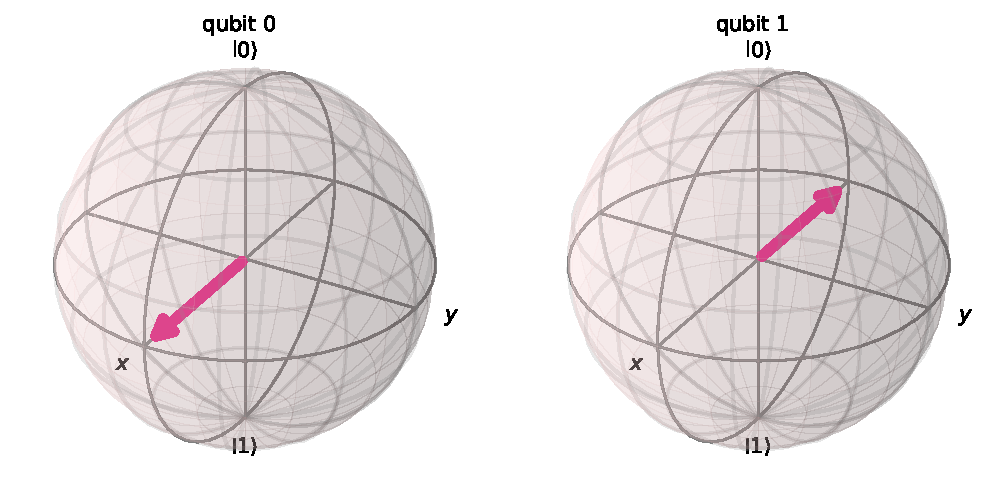
\includegraphics[keepaspectratio]{apostila_files/figure-pdf/cell-92-output-2.pdf}}

\pandocbounded{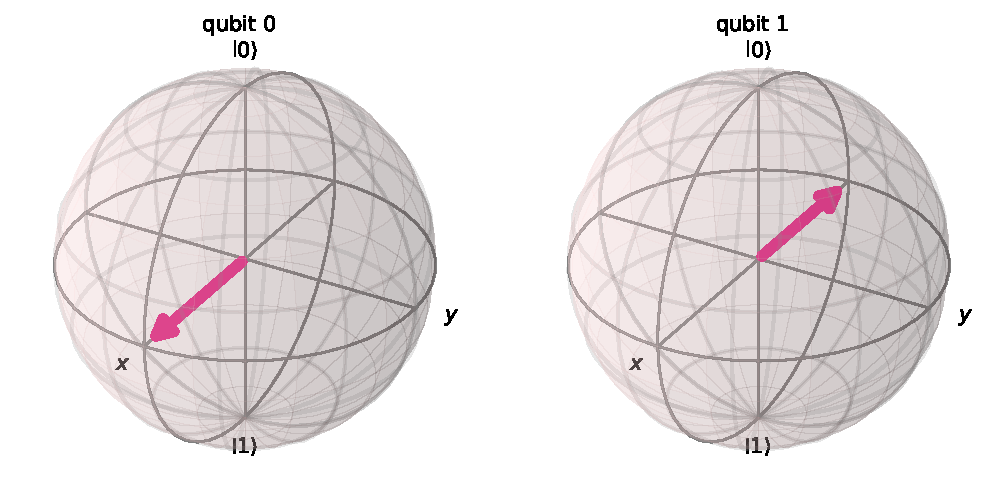
\includegraphics[keepaspectratio]{apostila_files/figure-pdf/cell-92-output-3.pdf}}

\begin{verbatim}
Estado inicial: Statevector([ 0.5+0.j,  0.5+0.j, -0.5+0.j, -0.5+0.j],
            dims=(2, 2))
\end{verbatim}

A esfera acima representa
\(|\psi_0\rangle = |+\rangle \otimes |-\rangle\).

\subsubsection{O que é a Esfera de
Bloch?}\label{o-que-uxe9-a-esfera-de-bloch}

(Relembrando)

A \textbf{Esfera de Bloch} é uma representação geométrica tridimensional
do estado de um único qubit. Ela é uma ferramenta visual poderosa para
entender os estados quânticos e suas transformações.

\textbf{Características principais:}

\begin{enumerate}
\def\labelenumi{\arabic{enumi}.}
\tightlist
\item
  \textbf{Polos da esfera:}

  \begin{itemize}
  \tightlist
  \item
    \textbf{Polo Norte (topo):} Representa o estado \(|0\rangle\)
  \item
    \textbf{Polo Sul (base):} Representa o estado \(|1\rangle\)
  \end{itemize}
\item
  \textbf{Equador da esfera:}

  \begin{itemize}
  \tightlist
  \item
    Contém todos os estados de superposição com fase relativa
  \item
    O ponto no eixo X positivo representa
    \(H|0\rangle = |+ \rangle = \frac{|0\rangle + |1\rangle}{\sqrt{2}}\)
  \item
    O ponto no eixo X negativo representa
    \(H|1\rangle = |-\rangle = \frac{|0\rangle - |1\rangle}{\sqrt{2}}\)
  \end{itemize}
\item
  \textbf{Interior da esfera:}

  \begin{itemize}
  \tightlist
  \item
    Apenas a superfície é válida para estados quânticos puros
  \item
    Pontos no interior representam estados mistos (não se aplicam aqui)
  \end{itemize}
\item
  \textbf{Vetores (setas rosa):}

  \begin{itemize}
  \tightlist
  \item
    Mostram o estado atual de cada qubit
  \item
    A direção do vetor indica a combinação de amplitude e fase
  \item
    Quanto mais próximo de um polo, maior a probabilidade de medir
    aquele estado
  \end{itemize}
\end{enumerate}

\textbf{Por que dois qubits = duas esferas?}

Cada qubit individual pode ser visualizado em sua própria esfera de
Bloch. Quando temos 2 qubits: - \textbf{Qubit 0 (esquerda):} Mostra o
estado do qubit de controle - \textbf{Qubit 1 (direita):} Mostra o
estado do qubit alvo

\textbf{Interpretando o estado preparado
(\(|+\rangle \otimes |-\rangle\)):}

\begin{itemize}
\tightlist
\item
  \textbf{Qubit 0:} O vetor aponta para o eixo X positivo → está em
  \(|+\rangle\)

  \begin{itemize}
  \tightlist
  \item
    Superposição igual entre \(|0\rangle\) e \(|1\rangle\) com fase
    positiva
  \item
    Probabilidades: 50\% de medir 0, 50\% de medir 1
  \end{itemize}
\item
  \textbf{Qubit 1:} O vetor aponta para o eixo X negativo → está em
  \(|-\rangle\)

  \begin{itemize}
  \tightlist
  \item
    Superposição igual entre \(|0\rangle\) e \(|1\rangle\) com fase
    negativa
  \item
    Probabilidades: 50\% de medir 0, 50\% de medir 1
  \item
    O sinal negativo é uma diferença de fase de 180° entre os
    componentes
  \end{itemize}
\end{itemize}

\textbf{O que observar nas visualizações:}

Quando aplicarmos o CNOT (Phase Kickback), veremos: - \textbf{Qubit 0:}
O vetor vai \textbf{girar} do eixo X+ para o eixo X- (de \(|+\rangle\)
para \(|-\rangle\)) - \textbf{Qubit 1:} O vetor \textbf{permanece no
mesmo lugar} (continua em \(|-\rangle\))

Essa rotação do qubit de controle \textbf{sem que nenhuma porta aja
diretamente sobre ele} é a essência do Phase Kickback!

\section{Q-Sphere}\label{q-sphere}

\begin{Shaded}
\begin{Highlighting}[]
\BuiltInTok{print}\NormalTok{(}\StringTok{"}\CharTok{\textbackslash{}n}\StringTok{Q{-}Sphere mostrando ambos os qubits:"}\NormalTok{)}
\NormalTok{display(plot\_state\_qsphere(estado\_inicial))}
\end{Highlighting}
\end{Shaded}

\begin{verbatim}

Q-Sphere mostrando ambos os qubits:
\end{verbatim}

\pandocbounded{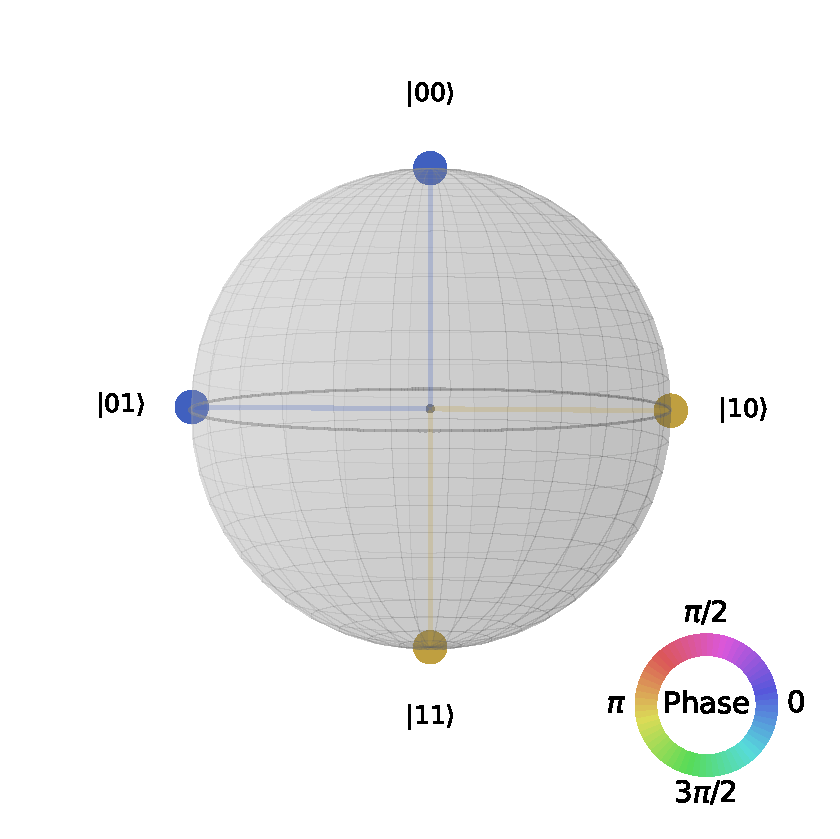
\includegraphics[keepaspectratio]{apostila_files/figure-pdf/cell-93-output-2.pdf}}

\pandocbounded{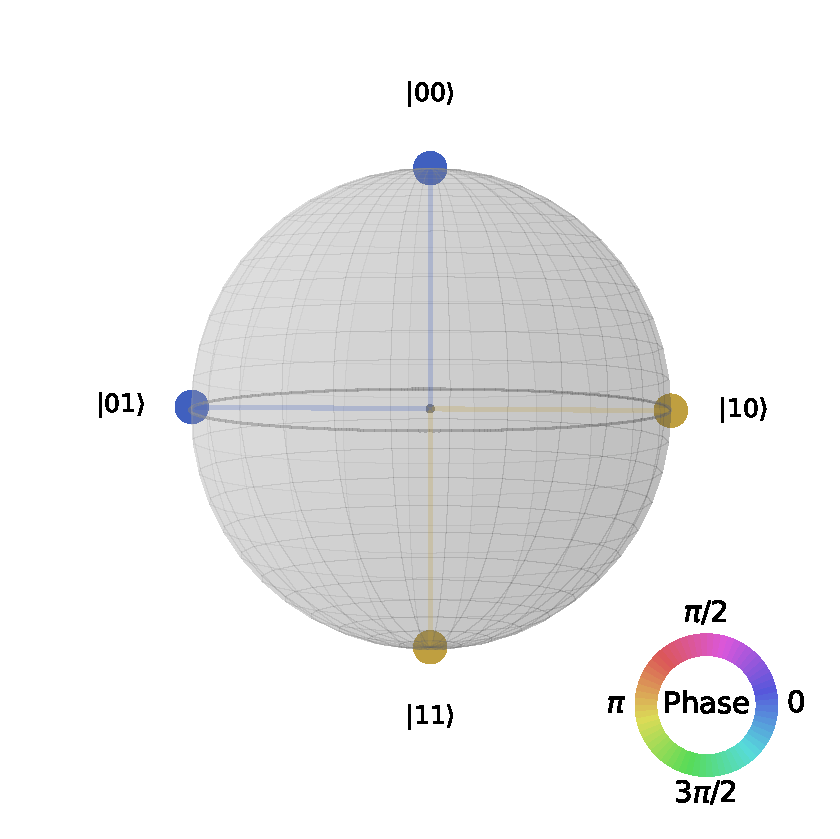
\includegraphics[keepaspectratio]{apostila_files/figure-pdf/cell-93-output-3.pdf}}

\begin{verbatim}

Q-Sphere mostrando ambos os qubits:
\end{verbatim}

\subsubsection{O que é a Q-Sphere (Esfera
Quântica)?}\label{o-que-uxe9-a-q-sphere-esfera-quuxe2ntica}

A \textbf{Q-Sphere} é outra visualização poderosa para sistemas
quânticos, especialmente útil para visualizar múltiplos qubits
simultaneamente. Diferente da Esfera de Bloch que mostra qubits
individuais, a Q-Sphere mostra o \textbf{estado completo do sistema}.

\textbf{Características principais:}

\begin{enumerate}
\def\labelenumi{\arabic{enumi}.}
\tightlist
\item
  \textbf{Estrutura da esfera:}

  \begin{itemize}
  \tightlist
  \item
    Cada \textbf{ponto na superfície} representa um possível estado da
    base computacional
  \item
    Para 2 qubits: 4 pontos (\textbar00⟩, \textbar01⟩, \textbar10⟩,
    \textbar11⟩)
  \item
    Para 3 qubits: 8 pontos (\textbar000⟩, \textbar001⟩, \textbar010⟩,
    \textbar011⟩, \textbar100⟩, \textbar101⟩, \textbar110⟩,
    \textbar111⟩)
  \end{itemize}
\item
  \textbf{Tamanho das esferas (círculos):}

  \begin{itemize}
  \tightlist
  \item
    O \textbf{diâmetro de cada círculo} representa a \textbf{amplitude}
    (probabilidade) daquele estado
  \item
    Círculos maiores = maior probabilidade de medir aquele estado
  \item
    Círculos menores = menor probabilidade
  \item
    Sem círculo = amplitude zero (não contribui para o estado)
  \end{itemize}
\item
  \textbf{Cores dos círculos:}

  \begin{itemize}
  \tightlist
  \item
    Representam a \textbf{fase} do estado quântico
  \item
    \textbf{Rosa/Magenta}: Fase positiva (0°)
  \item
    \textbf{Verde/Ciano}: Fase negativa (180°) ou outras fases
    intermediárias
  \item
    A cor indica a fase relativa entre os diferentes componentes do
    estado
  \end{itemize}
\item
  \textbf{Posição na esfera:}

  \begin{itemize}
  \tightlist
  \item
    A distribuição dos pontos na superfície segue uma convenção
    geométrica
  \item
    Estados relacionados ficam próximos na esfera
  \end{itemize}
\end{enumerate}

\textbf{Interpretando o estado \(|+\rangle \otimes |-\rangle\):}

Expandindo matematicamente:
\[|+\rangle \otimes |-\rangle = \frac{1}{2}(|00\rangle - |01\rangle + |10\rangle - |11\rangle)\]

Na Q-Sphere, veremos \textbf{4 círculos} de tamanhos iguais: -
\textbf{\textbar00⟩}: Amplitude \(\frac{1}{2}\), fase positiva (+) →
círculo rosa - \textbf{\textbar01⟩}: Amplitude \(\frac{1}{2}\), fase
negativa (-) → círculo verde/ciano - \textbf{\textbar10⟩}: Amplitude
\(\frac{1}{2}\), fase positiva (+) → círculo rosa -
\textbf{\textbar11⟩}: Amplitude \(\frac{1}{2}\), fase negativa (-) →
círculo verde/ciano

Todos os círculos têm o \textbf{mesmo tamanho} porque
\(|\frac{1}{2}|^2 = \frac{1}{4}\) (cada estado tem 25\% de probabilidade
de ser medido).

As \textbf{cores alternadas} mostram o padrão de fase: positivo para
\textbar00⟩ e \textbar10⟩, negativo para \textbar01⟩ e \textbar11⟩.

\textbf{Q-Sphere vs Esfera de Bloch:}

\begin{longtable}[]{@{}
  >{\raggedright\arraybackslash}p{(\linewidth - 2\tabcolsep) * \real{0.3846}}
  >{\raggedright\arraybackslash}p{(\linewidth - 2\tabcolsep) * \real{0.6154}}@{}}
\toprule\noalign{}
\begin{minipage}[b]{\linewidth}\raggedright
Q-Sphere
\end{minipage} & \begin{minipage}[b]{\linewidth}\raggedright
Esfera de Bloch
\end{minipage} \\
\midrule\noalign{}
\endhead
\bottomrule\noalign{}
\endlastfoot
Mostra o sistema completo (todos os qubits juntos) & Mostra cada qubit
individualmente \\
Revela correlações e emaranhamento & Limitada a 1 qubit por esfera \\
Exibe todas as amplitudes e fases simultaneamente & Mostra apenas o
estado reduzido de um qubit \\
Ideal para ver interferência quântica & Ideal para visualizar
transformações de um único qubit \\
\end{longtable}

\textbf{O que observar nas visualizações:}

Quando aplicarmos o CNOT (Phase Kickback), na Q-Sphere veremos: - Os
\textbf{tamanhos dos círculos permanecerão os mesmos} (probabilidades
não mudam) - As \textbf{cores mudarão} em alguns estados (as fases serão
alteradas) - Especificamente, veremos uma reorganização do padrão de
cores mostrando que a fase do sistema mudou

Essa mudança de fase sem alterar probabilidades é a assinatura
característica do \textbf{Phase Kickback}!

\begin{Shaded}
\begin{Highlighting}[]
\CommentTok{\# 🌐 Visualização INTERATIVA da Q{-}Sphere}
\CommentTok{\# Importar a função do módulo quantum\_viz (localizado em ../src)}
\ImportTok{import}\NormalTok{ sys}
\ImportTok{from}\NormalTok{ pathlib }\ImportTok{import}\NormalTok{ Path}
\ControlFlowTok{for}\NormalTok{ p }\KeywordTok{in}\NormalTok{ [Path.cwd(), Path.cwd().parent, Path.cwd().parent.parent]:}
    \ControlFlowTok{if}\NormalTok{ (p }\OperatorTok{/} \StringTok{"src"}\NormalTok{).is\_dir() }\KeywordTok{and} \BuiltInTok{str}\NormalTok{(p }\OperatorTok{/} \StringTok{"src"}\NormalTok{) }\KeywordTok{not} \KeywordTok{in}\NormalTok{ sys.path:}
\NormalTok{        sys.path.insert(}\DecValTok{0}\NormalTok{, }\BuiltInTok{str}\NormalTok{(p }\OperatorTok{/} \StringTok{"src"}\NormalTok{))}
\ImportTok{from}\NormalTok{ quantum\_viz }\ImportTok{import}\NormalTok{ plot\_qsphere\_interactive}

\CommentTok{\# 🎨 Criar e exibir a visualização}
\BuiltInTok{print}\NormalTok{(}\StringTok{"}\CharTok{\textbackslash{}n}\StringTok{🌐 Q{-}Sphere INTERATIVA:"}\NormalTok{)}
\BuiltInTok{print}\NormalTok{(}\StringTok{"   → Magenta = Fase positiva (+)"}\NormalTok{)}
\BuiltInTok{print}\NormalTok{(}\StringTok{"   → Ciano = Fase negativa ({-})"}\NormalTok{)}
\BuiltInTok{print}\NormalTok{(}\StringTok{"   → Tamanho = Probabilidade}\CharTok{\textbackslash{}n}\StringTok{"}\NormalTok{)}

\CommentTok{\# A função plot\_qsphere\_interactive salva automaticamente e abre no navegador}
\NormalTok{fig }\OperatorTok{=}\NormalTok{ plot\_qsphere\_interactive(estado\_inicial)}
\end{Highlighting}
\end{Shaded}

\begin{verbatim}

🌐 Q-Sphere INTERATIVA:
   → Magenta = Fase positiva (+)
   → Ciano = Fase negativa (-)
   → Tamanho = Probabilidade

✅ Visualização 3D salva em: /home/max/aula-quantum/content/qsphere_interativa.html
\end{verbatim}

\begin{verbatim}

🌐 Q-Sphere INTERATIVA:
   → Magenta = Fase positiva (+)
   → Ciano = Fase negativa (-)
   → Tamanho = Probabilidade

✅ Visualização 3D salva em: e:\temp\quantum\notebooks\qsphere_interativa.html
   Abrindo no navegador...

💡 Dica: Você pode arrastar, girar e dar zoom na esfera!
   O arquivo HTML pode ser aberto a qualquer momento.
\end{verbatim}

\begin{Shaded}
\begin{Highlighting}[]
\CommentTok{\# 2. O KICKBACK}
\CommentTok{\# Aplicamos CNOT. O alvo (q1) está em |{-}\textgreater{}.}
\CommentTok{\# Isso deve fazer o q0 virar |{-}\textgreater{} "por tabela".}
\NormalTok{qc.cx(}\DecValTok{0}\NormalTok{, }\DecValTok{1}\NormalTok{)}
\end{Highlighting}
\end{Shaded}

\begin{verbatim}
<qiskit.circuit.instructionset.InstructionSet at 0x7779ea49b0a0>
\end{verbatim}

\subsubsection{Demonstração Matemática: O Phase
Kickback}\label{demonstrauxe7uxe3o-matemuxe1tica-o-phase-kickback}

Aplicando CNOT ao estado \(|\psi_0\rangle\):

A porta CNOT age como:
\(\text{CNOT}|c,t\rangle = |c, c \oplus t\rangle\)

Mas quando o alvo está em \(|-\rangle\), temos uma propriedade especial:

\[\text{CNOT}|c\rangle \otimes |-\rangle = (-1)^c |c\rangle \otimes |-\rangle\]

Aplicando ao nosso estado:

\[|\psi_1\rangle = \text{CNOT}|\psi_0\rangle = \text{CNOT}\left[\frac{1}{\sqrt{2}}(|0\rangle + |1\rangle) \otimes |-\rangle\right]\]

\[= \frac{1}{\sqrt{2}}[\text{CNOT}(|0\rangle \otimes |-\rangle) + \text{CNOT}(|1\rangle \otimes |-\rangle)]\]

\[= \frac{1}{\sqrt{2}}[|0\rangle \otimes |-\rangle + (-1)|1\rangle \otimes |-\rangle]\]

\[= \frac{1}{\sqrt{2}}(|0\rangle - |1\rangle) \otimes |-\rangle = |-\rangle \otimes |-\rangle\]

\textbf{Conclusão:} O qubit de controle mudou de \(|+\rangle\) para
\(|-\rangle\) sem que nenhuma porta tenha agido diretamente sobre ele!

\begin{Shaded}
\begin{Highlighting}[]
\CommentTok{\# Visualizar após o CNOT (Phase Kickback aconteceu)}
\NormalTok{estado\_apos\_kickback }\OperatorTok{=}\NormalTok{ Statevector(qc)}
\BuiltInTok{print}\NormalTok{(}\SpecialStringTok{f"Estado após CNOT: }\SpecialCharTok{\{}\NormalTok{estado\_apos\_kickback}\SpecialCharTok{\}}\SpecialStringTok{"}\NormalTok{)}
\BuiltInTok{print}\NormalTok{(}\StringTok{"}\CharTok{\textbackslash{}n}\StringTok{Esfera de Bloch {-} Note a mudança de fase no qubit 0:"}\NormalTok{)}
\NormalTok{display(plot\_bloch\_multivector(estado\_apos\_kickback))}
\BuiltInTok{print}\NormalTok{(}\StringTok{"}\CharTok{\textbackslash{}n}\StringTok{Q{-}Sphere:"}\NormalTok{)}
\NormalTok{display(plot\_state\_qsphere(estado\_apos\_kickback))}
\end{Highlighting}
\end{Shaded}

\begin{verbatim}
Estado após CNOT: Statevector([ 0.5+0.j, -0.5+0.j, -0.5+0.j,  0.5+0.j],
            dims=(2, 2))

Esfera de Bloch - Note a mudança de fase no qubit 0:
\end{verbatim}

\pandocbounded{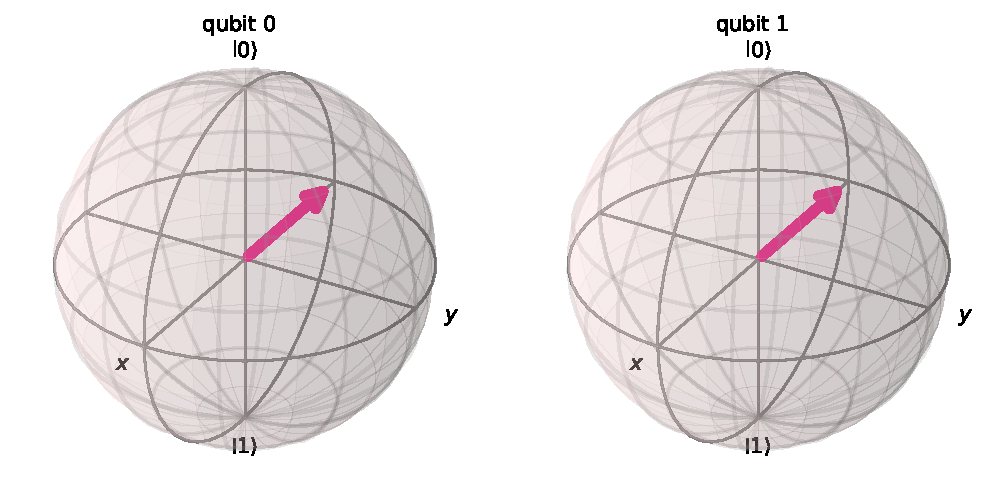
\includegraphics[keepaspectratio]{apostila_files/figure-pdf/cell-96-output-2.pdf}}

\begin{verbatim}

Q-Sphere:
\end{verbatim}

\pandocbounded{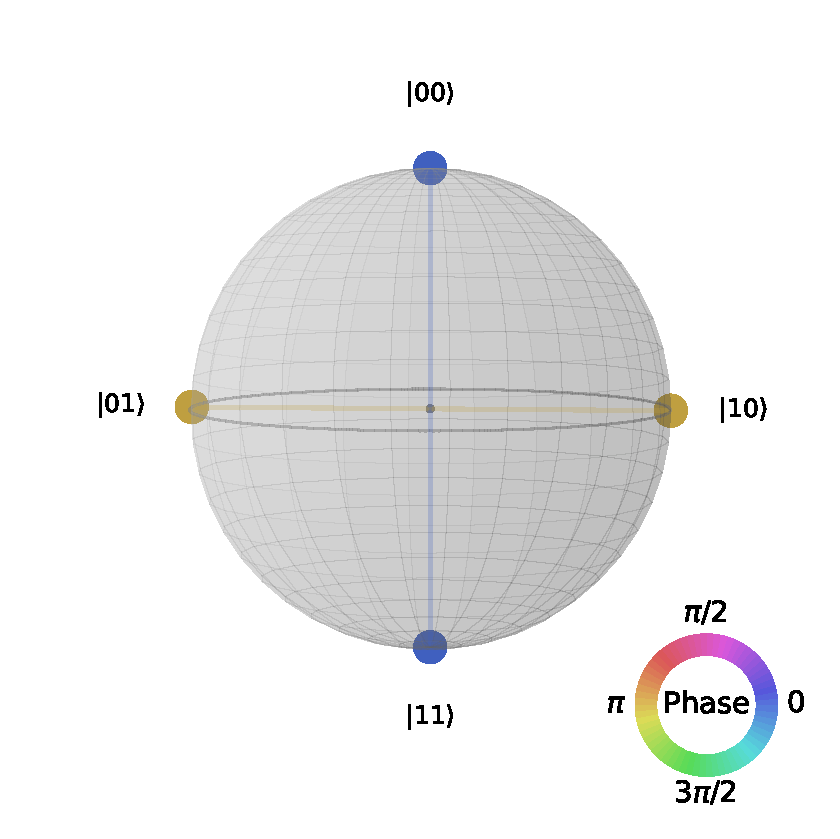
\includegraphics[keepaspectratio]{apostila_files/figure-pdf/cell-96-output-4.pdf}}

\pandocbounded{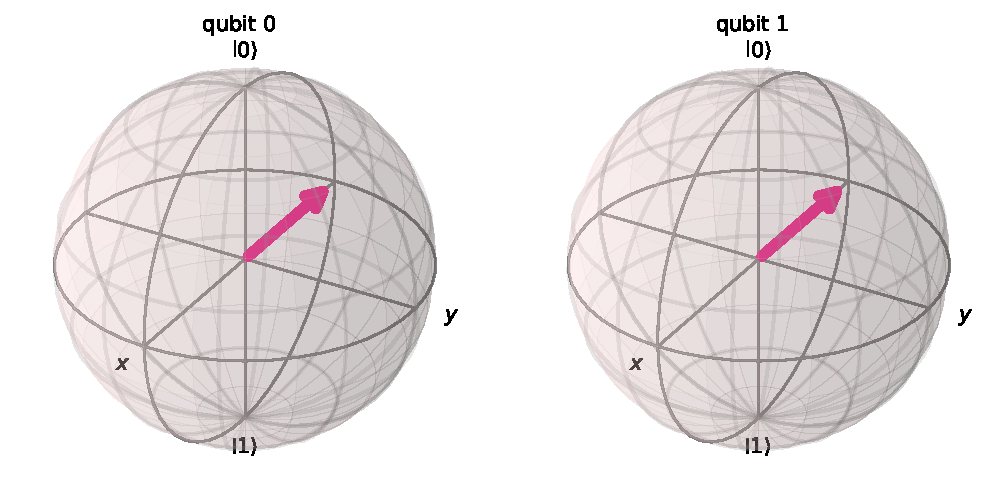
\includegraphics[keepaspectratio]{apostila_files/figure-pdf/cell-96-output-5.pdf}}

\pandocbounded{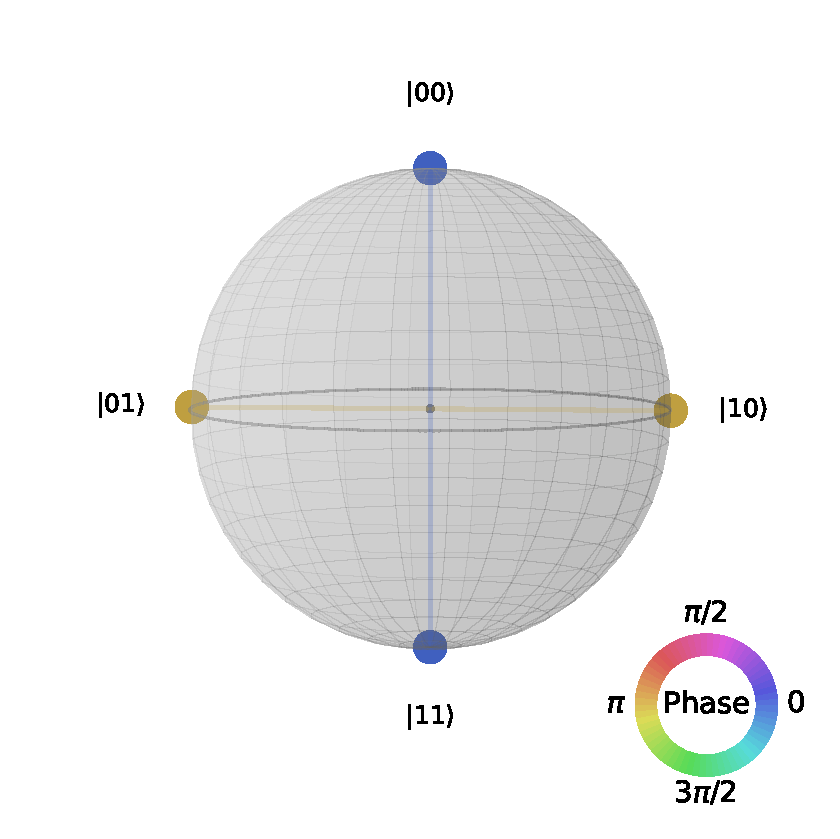
\includegraphics[keepaspectratio]{apostila_files/figure-pdf/cell-96-output-6.pdf}}

\begin{verbatim}
Estado após CNOT: Statevector([ 0.5+0.j, -0.5+0.j, -0.5+0.j,  0.5+0.j],
            dims=(2, 2))

Esfera de Bloch - Note a mudança de fase no qubit 0:
\end{verbatim}

\begin{verbatim}

Q-Sphere:
\end{verbatim}

\subsubsection{Visualização: Após o Phase Kickback
(CNOT)}\label{visualizauxe7uxe3o-apuxf3s-o-phase-kickback-cnot}

\begin{Shaded}
\begin{Highlighting}[]
\CommentTok{\# 3. VERIFICAÇÃO}
\CommentTok{\# Como saber se q0 virou |{-}\textgreater{}?}
\CommentTok{\# Se aplicarmos H novamente:}
\CommentTok{\# H em |+\textgreater{} volta para 0}
\CommentTok{\# H em |{-}\textgreater{} volta para 1}
\NormalTok{qc.h(}\DecValTok{0}\NormalTok{)}
\end{Highlighting}
\end{Shaded}

\begin{verbatim}
<qiskit.circuit.instructionset.InstructionSet at 0x7779dbf15a50>
\end{verbatim}

\subsubsection{Demonstração Matemática: Verificação com
Hadamard}\label{demonstrauxe7uxe3o-matemuxe1tica-verificauxe7uxe3o-com-hadamard}

Para verificar que o qubit 0 está em \(|-\rangle\), aplicamos H
novamente:

\[H|+\rangle = H \cdot H|0\rangle = |0\rangle\]

\[H|-\rangle = H \cdot H|1\rangle = |1\rangle\]

Portanto: - Se medirmos \textbf{0}, o estado antes era \(|+\rangle\) -
Se medirmos \textbf{1}, o estado antes era \(|-\rangle\)

Como o Phase Kickback transformou \(|+\rangle \to |-\rangle\), esperamos
medir \textbf{1} em 100\% das vezes!

\begin{Shaded}
\begin{Highlighting}[]
\NormalTok{estado\_verificacao }\OperatorTok{=}\NormalTok{ Statevector(qc)}
\BuiltInTok{print}\NormalTok{(}\SpecialStringTok{f"Estado após verificação (H no q0): }\SpecialCharTok{\{}\NormalTok{estado\_verificacao}\SpecialCharTok{\}}\SpecialStringTok{"}\NormalTok{)}
\NormalTok{display(plot\_bloch\_multivector(estado\_verificacao))}
\BuiltInTok{print}\NormalTok{(}\StringTok{"}\CharTok{\textbackslash{}n}\StringTok{Q{-}Sphere:"}\NormalTok{)}
\NormalTok{display(plot\_state\_qsphere(estado\_verificacao))}
\end{Highlighting}
\end{Shaded}

\begin{verbatim}
Estado após verificação (H no q0): Statevector([ 2.29934717e-17+0.j,  7.07106781e-01+0.j, -2.29934717e-17+0.j,
             -7.07106781e-01+0.j],
            dims=(2, 2))
\end{verbatim}

\pandocbounded{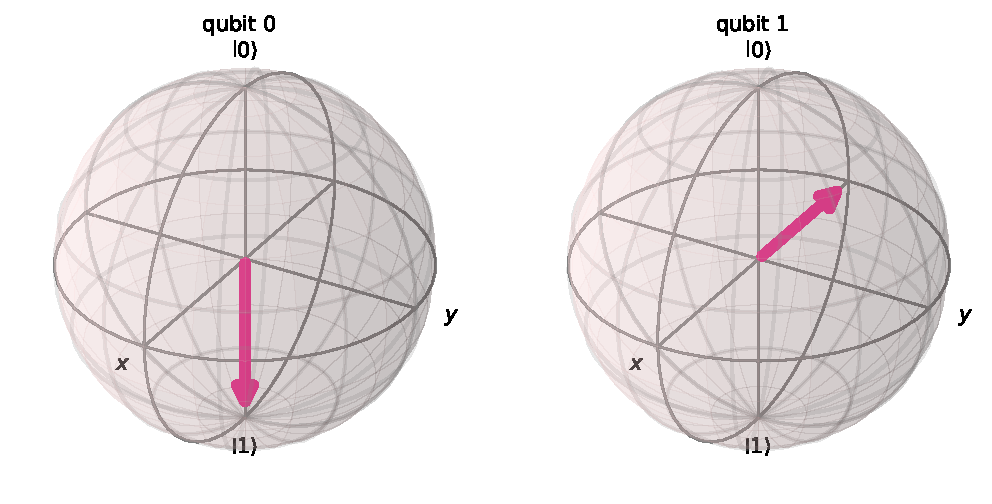
\includegraphics[keepaspectratio]{apostila_files/figure-pdf/cell-98-output-2.pdf}}

\begin{verbatim}

Q-Sphere:
\end{verbatim}

\pandocbounded{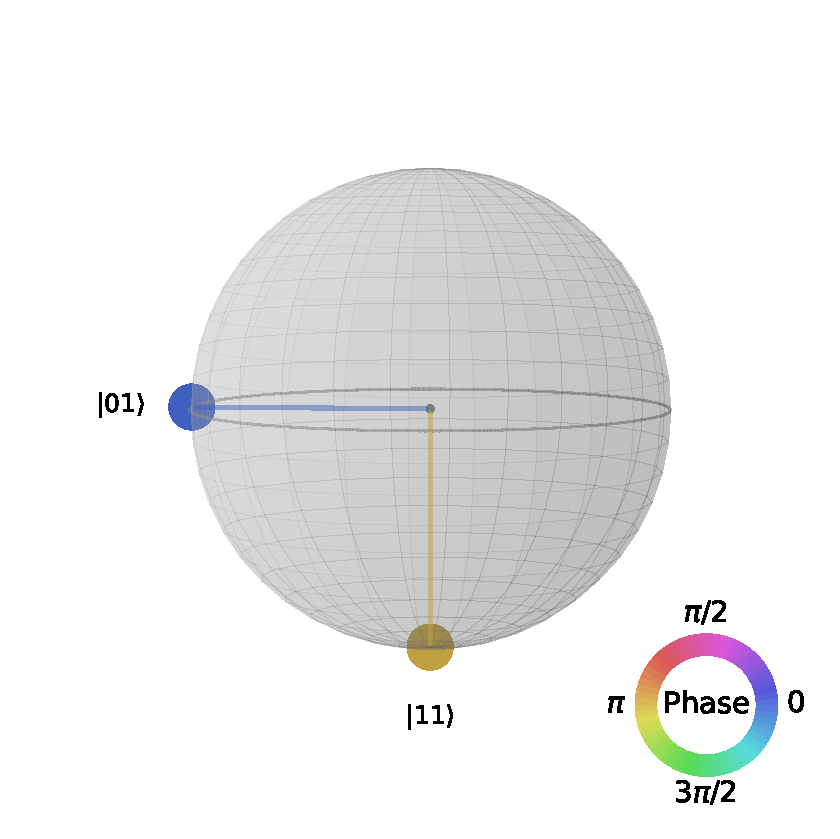
\includegraphics[keepaspectratio]{apostila_files/figure-pdf/cell-98-output-4.pdf}}

\pandocbounded{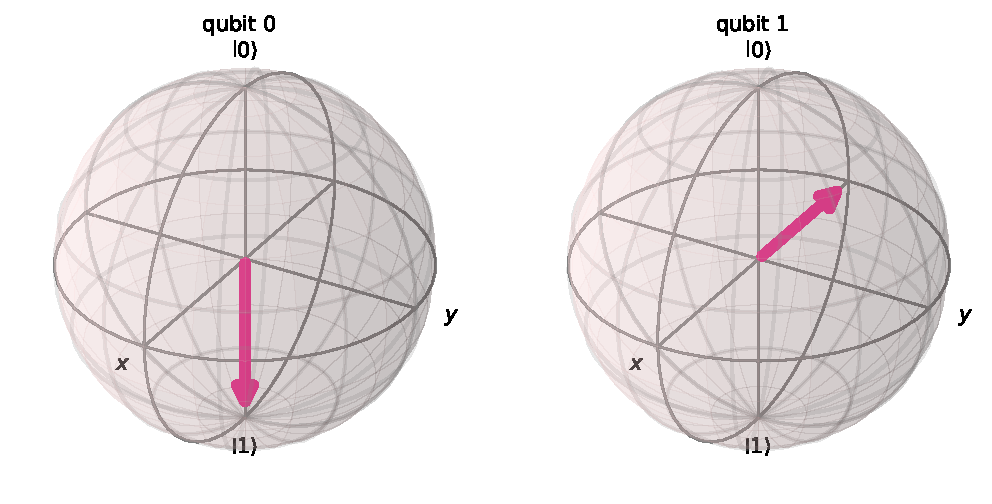
\includegraphics[keepaspectratio]{apostila_files/figure-pdf/cell-98-output-5.pdf}}

\pandocbounded{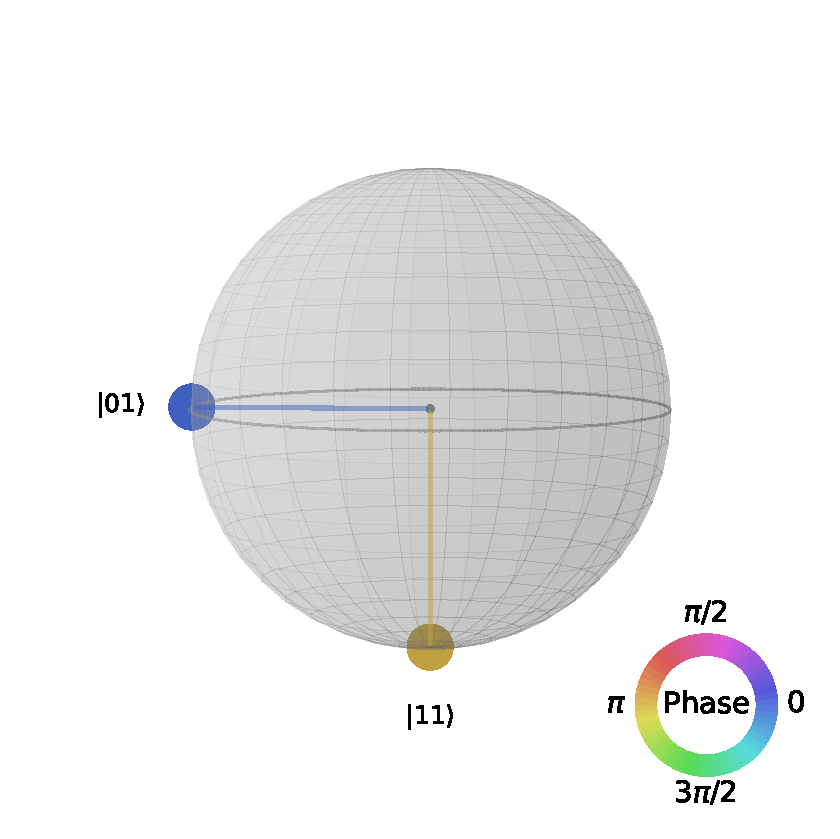
\includegraphics[keepaspectratio]{apostila_files/figure-pdf/cell-98-output-6.pdf}}

\begin{verbatim}
Estado após verificação (H no q0): Statevector([ 2.29934717e-17+0.j,  7.07106781e-01+0.j, -2.29934717e-17+0.j,
             -7.07106781e-01+0.j],
            dims=(2, 2))
\end{verbatim}

\begin{verbatim}

Q-Sphere:
\end{verbatim}

\begin{Shaded}
\begin{Highlighting}[]
\CommentTok{\# Medimos APENAS o qubit de controle (q0)}
\NormalTok{qc.measure(}\DecValTok{0}\NormalTok{, }\DecValTok{0}\NormalTok{)}

\CommentTok{\# Executar}
\NormalTok{simulador }\OperatorTok{=}\NormalTok{ AerSimulator()}
\NormalTok{job }\OperatorTok{=}\NormalTok{ simulador.run(transpile(qc, simulador), shots}\OperatorTok{=}\DecValTok{1000}\NormalTok{)}
\BuiltInTok{print}\NormalTok{(}\StringTok{"Resultado do Controle:"}\NormalTok{, job.result().get\_counts())}
\end{Highlighting}
\end{Shaded}

\begin{verbatim}
Resultado do Controle: {'1': 1000}
\end{verbatim}

\begin{verbatim}
Resultado do Controle: {'1': 1000}
\end{verbatim}

\textbf{Resultado esperado:}
\texttt{\{\textquotesingle{}1\textquotesingle{}:\ 1000\}}. Você mediu 1.
Isso prova que o estado antes da medição era \(\ket{1}\). O controle foi
alterado pelo alvo!

\subsection{2. O Algoritmo de
Deutsch-Jozsa}\label{o-algoritmo-de-deutsch-jozsa}

Agora vamos usar esse ``coice'' para resolver um problema.

\textbf{O problema}: Você tem uma função secreta (uma caixa preta)
\(f(x)\) que recebe bits e cospe 0 ou 1. Você sabe que a função só pode
ser de dois tipos:

\begin{enumerate}
\def\labelenumi{\arabic{enumi}.}
\tightlist
\item
  \textbf{Constante:} Retorna sempre 0 ou sempre 1 (independente da
  entrada).
\item
  \textbf{Balanceada:} Retorna 0 para metade das entradas e 1 para a
  outra metade.
\end{enumerate}

Para ser mais intuitivo:

\begin{enumerate}
\def\labelenumi{\arabic{enumi}.}
\tightlist
\item
  Imagine que você implemente um vetor com 3 bits de entrada (000 a
  111): \texttt{vetor\ =\ {[}0,\ 1,\ 0{]}} por exemplo.
\item
  Se o vetor for \texttt{{[}0,0,0{]}}, isto é, todos os valores são 0,
  então a função é \textbf{constante}.
\item
  Se o vetor for \texttt{{[}1,1,1{]}}, isto é, todos os valores são 1,
  então a função é \textbf{constante}.
\item
  Se o vetor for \texttt{{[}0,1,1{]}}, isto é, alguns dos valores são 0
  e outros são 1, então a função é \textbf{balanceada}.
\item
  A função \(f(x)\) verifica se o vetor é constante ou balanceado.
\item
  Somente isso.
\end{enumerate}

\textbf{Desafio:} Quantas vezes você precisa testar a caixa para ter
100\% de certeza de qual tipo ela é?

\begin{itemize}
\tightlist
\item
  \textbf{Computador Clássico:} Se a entrada tem 3 bits, você precisa
  testar pelo menos \(2^{3-1} + 1 = 5\) vezes.
\item
  \textbf{Computador Quântico:} \textbf{1 vez.} (Não importa se são 3
  bits ou 1 milhão de bits).
\end{itemize}

Vamos ver na prática se isso é verdade?

\subsubsection{Teste com 3 bits em computador
clássico}\label{teste-com-3-bits-em-computador-cluxe1ssico}

Para os curiosos, resolvi criar à parte o problema da caixa preta para
ser utilizado em um computador clássico. Segue o código:

\begin{Shaded}
\begin{Highlighting}[]
\ImportTok{import}\NormalTok{ random}

\KeywordTok{def}\NormalTok{ eh\_constante\_ou\_balanceada(tabela\_oculta):}
    \CommentTok{"""}
\CommentTok{    Entra um vetor parecido com [0,1,0,1,1], este com 5 bits, por exemplo.}
\CommentTok{    Procura saber se o vetor é constante (só tem 0s ou 1s) ou balanceada (tem 0s e 1s misturados)}
\CommentTok{    """}
\NormalTok{    historico\_saidas }\OperatorTok{=}\NormalTok{ []}
    
    \CommentTok{\# Testar até o limite do pior caso}
    \ControlFlowTok{for}\NormalTok{ i }\KeywordTok{in} \BuiltInTok{range}\NormalTok{(limite\_pior\_caso):}
        \BuiltInTok{print}\NormalTok{(}\SpecialStringTok{f"Input: }\SpecialCharTok{\{}\NormalTok{i}\SpecialCharTok{:03b\}}\SpecialStringTok{ {-}\textgreater{} Output: }\SpecialCharTok{\{}\NormalTok{tabela\_oculta[i]}\SpecialCharTok{\}}\SpecialStringTok{"}\NormalTok{)}
\NormalTok{        historico\_saidas.append(tabela\_oculta[i])}
        
        \CommentTok{\# Se a lista tiver somente 0s ou somente 1s, continuar}
        \CommentTok{\# Caso contrário, já sabemos que é balanceada}
        \ControlFlowTok{if} \DecValTok{0} \KeywordTok{in}\NormalTok{ historico\_saidas }\KeywordTok{and} \DecValTok{1} \KeywordTok{in}\NormalTok{ historico\_saidas:}
            \BuiltInTok{print}\NormalTok{(}\StringTok{"Achamos ambos os valores! A função é balanceada."}\NormalTok{)}
            \ControlFlowTok{return} \StringTok{"Balanceada"}
    
    \BuiltInTok{print}\NormalTok{(}\StringTok{"Todos os valores são iguais! A função é constante."}\NormalTok{)}
    \ControlFlowTok{return} \StringTok{"Constante"}

\CommentTok{\# Utilizando inicialmente 3 bits de entrada (000) para execução rápida e}
\CommentTok{\# simplificação. Experimente depois aumentar para 15 bits. Você verá }
\CommentTok{\# como é lentooo...}
\NormalTok{n\_bits }\OperatorTok{=} \DecValTok{3}

\CommentTok{\# Número total de entradas possíveis (2\^{}n\_bits)}
\NormalTok{total\_inputs }\OperatorTok{=} \DecValTok{2} \OperatorTok{**}\NormalTok{ n\_bits}

\CommentTok{\# Vamos fazer o teste contante aqui}
\NormalTok{tabela\_oculta }\OperatorTok{=}\NormalTok{ []                          }\CommentTok{\# Lista que representa a função oculta}
\NormalTok{valor }\OperatorTok{=}\NormalTok{ random.choice([}\DecValTok{0}\NormalTok{, }\DecValTok{1}\NormalTok{])               }\CommentTok{\# Escolhe aleatoriamente 0 ou 1 para toda a lista}
\NormalTok{tabela\_oculta }\OperatorTok{=}\NormalTok{ [valor] }\OperatorTok{*}\NormalTok{ total\_inputs      }\CommentTok{\# Preenche a lista com o valor escolhido}

\BuiltInTok{print}\NormalTok{(}\StringTok{"Tabela oculta (caixa preta):"}\NormalTok{)}
\BuiltInTok{print}\NormalTok{(tabela\_oculta)                        }\CommentTok{\# Exibe a tabela oculta}

\NormalTok{limite\_pior\_caso }\OperatorTok{=}\NormalTok{ (}\DecValTok{2} \OperatorTok{**}\NormalTok{ (n\_bits}\OperatorTok{{-}}\DecValTok{1}\NormalTok{)) }\OperatorTok{+} \DecValTok{1}    \CommentTok{\# Limite para o pior caso (metade + 1)}

\CommentTok{\# Aqui começa o teste}
\CommentTok{\# Deverá verificar se a função é constante ou balanceada}
\CommentTok{\# Se todos os valores forem iguais, é constante}
\CommentTok{\# Se encontrar ambos os valores (0 e 1) dentro da lista, é balanceada.}
\CommentTok{\# Obviamente vai ser contante, pois preenchemos assim.}

\BuiltInTok{print}\NormalTok{(}\StringTok{"}\CharTok{\textbackslash{}n}\StringTok{Testando se a função é constante ou balanceada:"}\NormalTok{)}
\NormalTok{eh\_constante\_ou\_balanceada(tabela\_oculta)}
    
\CommentTok{\# Agora vamos fazer o teste balanceado}
\NormalTok{tabela\_oculta }\OperatorTok{=}\NormalTok{ []                          }\CommentTok{\# Resetar a lista}
\NormalTok{metade }\OperatorTok{=}\NormalTok{ total\_inputs }\OperatorTok{//} \DecValTok{2}                  \CommentTok{\# Calcular a metade do total de entradas}
\NormalTok{tabela\_oculta }\OperatorTok{=}\NormalTok{ [}\DecValTok{0}\NormalTok{] }\OperatorTok{*}\NormalTok{ metade }\OperatorTok{+}\NormalTok{ [}\DecValTok{1}\NormalTok{] }\OperatorTok{*}\NormalTok{ metade }\CommentTok{\# Preencher metade com 0s e metade com 1s}
\NormalTok{random.shuffle(tabela\_oculta)               }\CommentTok{\# Embaralhar a lista para aleatoriedade}

\BuiltInTok{print}\NormalTok{(}\StringTok{"}\CharTok{\textbackslash{}n}\StringTok{Tabela oculta (caixa preta):"}\NormalTok{)}
\BuiltInTok{print}\NormalTok{(tabela\_oculta)                        }\CommentTok{\# Exibe a tabela oculta}

\BuiltInTok{print}\NormalTok{(}\StringTok{"}\CharTok{\textbackslash{}n}\StringTok{Testando se a função é constante ou balanceada:"}\NormalTok{)}
\NormalTok{eh\_constante\_ou\_balanceada(tabela\_oculta)}
\end{Highlighting}
\end{Shaded}

\begin{verbatim}
Tabela oculta (caixa preta):
[0, 0, 0, 0, 0, 0, 0, 0]

Testando se a função é constante ou balanceada:
Input: 000 -> Output: 0
Input: 001 -> Output: 0
Input: 010 -> Output: 0
Input: 011 -> Output: 0
Input: 100 -> Output: 0
Todos os valores são iguais! A função é constante.

Tabela oculta (caixa preta):
[1, 0, 0, 1, 0, 0, 1, 1]

Testando se a função é constante ou balanceada:
Input: 000 -> Output: 1
Input: 001 -> Output: 0
Achamos ambos os valores! A função é balanceada.
\end{verbatim}

\begin{verbatim}
'Balanceada'
\end{verbatim}

\begin{verbatim}
Tabela oculta (caixa preta):
[0, 0, 0, 0, 0, 0, 0, 0]

Testando se a função é constante ou balanceada:
Input: 000 -> Output: 0
Input: 001 -> Output: 0
Input: 010 -> Output: 0
Input: 011 -> Output: 0
Input: 100 -> Output: 0
Todos os valores são iguais! A função é constante.

Tabela oculta (caixa preta):
[0, 0, 1, 0, 1, 0, 1, 1]

Testando se a função é constante ou balanceada:
Input: 000 -> Output: 0
Input: 001 -> Output: 0
Input: 010 -> Output: 1
Achamos ambos os valores! A função é balanceada.
\end{verbatim}

O que observar ao rodar este código:

\begin{enumerate}
\def\labelenumi{\arabic{enumi}.}
\item
  \textbf{No Teste Constante}: O código sempre irá até a tentativa 5 (no
  caso de 3 bits).

  \begin{itemize}
  \tightlist
  \item
    Imagine que a função retorna sempre 0.
  \item
    Ao testar a entrada 1, 2, 3 e 4, você obteve 0, 0, 0, 0.
  \item
    Você ainda não pode parar. Por quê? Porque uma função balanceada
    poderia ter seus quatro zeros escondidos justamente nas quatro
    primeiras posições!
  \item
    Só ao testar a 5ª vez e obter 0, você prova matematicamente que não
    existem ``uns'' suficientes para ela ser balanceada.
  \end{itemize}
\item
  \textbf{No Teste Balanceado}: O código pode parar na tentativa 2 (se
  você tiver sorte de tirar um 0 e logo depois um 1), ou pode demorar
  até a tentativa 5 (se você tiver muito azar e tirar todos os 0s antes
  de achar um 1).
\end{enumerate}

➡️ Sei que é bem simples o código, mas tente rodar com 15 bits (altere
em \texttt{n\_bits}) para ver a diferença de tempo! Demora muito!!!

Este código é a prova prática da ineficiência do computador clássico que
o Algoritmo de Deutsch-Jozsa resolve com apenas uma consulta com
computador quântico!

\section{🚀 Versão Quântica do
Problema}\label{versuxe3o-quuxe2ntica-do-problema}

Agora vamos implementar o \textbf{Algoritmo de Deutsch-Jozsa} - a versão
quântica que resolve o mesmo problema com \textbf{apenas 1 consulta ao
oráculo}!

\begin{Shaded}
\begin{Highlighting}[]
\ImportTok{from}\NormalTok{ qiskit }\ImportTok{import}\NormalTok{ QuantumCircuit, transpile}
\ImportTok{from}\NormalTok{ qiskit\_aer }\ImportTok{import}\NormalTok{ AerSimulator}
\ImportTok{from}\NormalTok{ qiskit.quantum\_info }\ImportTok{import}\NormalTok{ Statevector}
\ImportTok{from}\NormalTok{ qiskit.visualization }\ImportTok{import}\NormalTok{ plot\_bloch\_multivector, plot\_state\_qsphere, plot\_histogram}
\end{Highlighting}
\end{Shaded}

\begin{Shaded}
\begin{Highlighting}[]
\CommentTok{\# ============================================}
\CommentTok{\# DEFINIÇÃO DOS ORÁCULOS}
\CommentTok{\# ============================================}

\KeywordTok{def}\NormalTok{ oraculo\_balanceado(n\_qubits):}
    \CommentTok{"""}
\CommentTok{    Cria um circuito que representa uma função BALANCEADA.}
\CommentTok{    }
\CommentTok{    Esta função retorna 0 para metade das entradas e 1 para a outra metade.}
\CommentTok{    Implementação: CNOTs de todos os qubits de entrada para o qubit de saída.}
\CommentTok{    }
\CommentTok{    Equivalente quântico de: tabela\_oculta = [0]*metade + [1]*metade (embaralhado)}
\CommentTok{    """}
\NormalTok{    qc }\OperatorTok{=}\NormalTok{ QuantumCircuit(n\_qubits }\OperatorTok{+} \DecValTok{1}\NormalTok{)}
    \ControlFlowTok{for}\NormalTok{ qubit }\KeywordTok{in} \BuiltInTok{range}\NormalTok{(n\_qubits):}
\NormalTok{        qc.cx(qubit, n\_qubits) }\CommentTok{\# CNOT de todos inputs para o alvo}
    \ControlFlowTok{return}\NormalTok{ qc}

\KeywordTok{def}\NormalTok{ oraculo\_constante(n\_qubits):}
    \CommentTok{"""}
\CommentTok{    Cria um circuito que representa uma função CONSTANTE.}
\CommentTok{    }
\CommentTok{    Esta função retorna sempre 0 ou sempre 1 (independente da entrada).}
\CommentTok{    }
\CommentTok{    Implementação:}
\CommentTok{    {-} Retorna sempre 0: não faz nada (circuito identidade)}
\CommentTok{    {-} Retorna sempre 1: aplica X no qubit de saída}
\CommentTok{    }
\CommentTok{    Equivalente quântico de: tabela\_oculta = [0] * total\_inputs}
\CommentTok{                          ou: tabela\_oculta = [1] * total\_inputs}
\CommentTok{    """}
\NormalTok{    qc }\OperatorTok{=}\NormalTok{ QuantumCircuit(n\_qubits }\OperatorTok{+} \DecValTok{1}\NormalTok{)}
    \CommentTok{\# Não adicionamos portas, então a saída é constante 0}
    \CommentTok{\# Para constante 1, descomente a linha abaixo:}
    \CommentTok{\# qc.x(n\_qubits)}
    \ControlFlowTok{return}\NormalTok{ qc}
\end{Highlighting}
\end{Shaded}

\begin{Shaded}
\begin{Highlighting}[]
\CommentTok{\# 🎮 EXPERIMENTO INTERATIVO: Teste Ambos os Tipos de Função}

\ImportTok{import}\NormalTok{ random}

\KeywordTok{def}\NormalTok{ executar\_deutsch\_jozsa(n\_bits, tipo\_funcao):}
    \CommentTok{"""}
\CommentTok{    Executa o Algoritmo de Deutsch{-}Jozsa para um tipo específico de função.}
\CommentTok{    }
\CommentTok{    Args:}
\CommentTok{        n\_bits: Número de bits de entrada}
\CommentTok{        tipo\_funcao: "constante" ou "balanceada"}
\CommentTok{    """}
\NormalTok{    qc }\OperatorTok{=}\NormalTok{ QuantumCircuit(n\_bits }\OperatorTok{+} \DecValTok{1}\NormalTok{, n\_bits)}
    
    \CommentTok{\# PASSO 1: Preparação}
    \ControlFlowTok{for}\NormalTok{ i }\KeywordTok{in} \BuiltInTok{range}\NormalTok{(n\_bits):}
\NormalTok{        qc.h(i)}
\NormalTok{    qc.x(n\_bits)}
\NormalTok{    qc.h(n\_bits)}
\NormalTok{    qc.barrier()}
    
    \CommentTok{\# PASSO 2: Aplicar oráculo}
    \ControlFlowTok{if}\NormalTok{ tipo\_funcao }\OperatorTok{==} \StringTok{"constante"}\NormalTok{:}
\NormalTok{        valor\_constante }\OperatorTok{=}\NormalTok{ random.choice([}\DecValTok{0}\NormalTok{, }\DecValTok{1}\NormalTok{])}
\NormalTok{        oraculo }\OperatorTok{=}\NormalTok{ oraculo\_constante(n\_bits)}
        \ControlFlowTok{if}\NormalTok{ valor\_constante }\OperatorTok{==} \DecValTok{1}\NormalTok{:}
\NormalTok{            oraculo.x(n\_bits)}
\NormalTok{        tipo\_real }\OperatorTok{=} \StringTok{"CONSTANTE"}
\NormalTok{        tabela\_classica }\OperatorTok{=}\NormalTok{ [valor\_constante] }\OperatorTok{*}\NormalTok{ (}\DecValTok{2}\OperatorTok{**}\NormalTok{n\_bits)}
    \ControlFlowTok{else}\NormalTok{:}
\NormalTok{        oraculo }\OperatorTok{=}\NormalTok{ oraculo\_balanceado(n\_bits)}
\NormalTok{        tipo\_real }\OperatorTok{=} \StringTok{"BALANCEADA"}
\NormalTok{        metade }\OperatorTok{=} \DecValTok{2}\OperatorTok{**}\NormalTok{(n\_bits}\OperatorTok{{-}}\DecValTok{1}\NormalTok{)}
\NormalTok{        tabela\_classica }\OperatorTok{=}\NormalTok{ [}\DecValTok{0}\NormalTok{]}\OperatorTok{*}\NormalTok{metade }\OperatorTok{+}\NormalTok{ [}\DecValTok{1}\NormalTok{]}\OperatorTok{*}\NormalTok{metade}
\NormalTok{        random.shuffle(tabela\_classica)}
    
\NormalTok{    qc }\OperatorTok{=}\NormalTok{ qc.compose(oraculo)}
\NormalTok{    qc.barrier()}
    
    \CommentTok{\# PASSO 3: Interferência}
    \ControlFlowTok{for}\NormalTok{ i }\KeywordTok{in} \BuiltInTok{range}\NormalTok{(n\_bits):}
\NormalTok{        qc.h(i)}
    
    \CommentTok{\# PASSO 4: Medição}
\NormalTok{    qc.measure(}\BuiltInTok{range}\NormalTok{(n\_bits), }\BuiltInTok{range}\NormalTok{(n\_bits))}
    
    \CommentTok{\# PASSO 5: Executar}
\NormalTok{    simulador }\OperatorTok{=}\NormalTok{ AerSimulator()}
\NormalTok{    job }\OperatorTok{=}\NormalTok{ simulador.run(transpile(qc, simulador), shots}\OperatorTok{=}\DecValTok{1}\NormalTok{)}
\NormalTok{    resultado }\OperatorTok{=}\NormalTok{ job.result().get\_counts()}
\NormalTok{    medicao }\OperatorTok{=} \BuiltInTok{list}\NormalTok{(resultado.keys())[}\DecValTok{0}\NormalTok{]}
    
    \CommentTok{\# Interpretar}
    \ControlFlowTok{if}\NormalTok{ medicao }\OperatorTok{==} \StringTok{\textquotesingle{}0\textquotesingle{}} \OperatorTok{*}\NormalTok{ n\_bits:}
\NormalTok{        resultado\_quantum }\OperatorTok{=} \StringTok{"CONSTANTE"}
    \ControlFlowTok{else}\NormalTok{:}
\NormalTok{        resultado\_quantum }\OperatorTok{=} \StringTok{"BALANCEADA"}
    
    \CommentTok{\# Exibir resultados}
    \BuiltInTok{print}\NormalTok{(}\StringTok{"="}\OperatorTok{*}\DecValTok{70}\NormalTok{)}
    \BuiltInTok{print}\NormalTok{(}\SpecialStringTok{f"🧪 TESTE COM FUNÇÃO }\SpecialCharTok{\{}\NormalTok{tipo\_real}\SpecialCharTok{\}}\SpecialStringTok{"}\NormalTok{)}
    \BuiltInTok{print}\NormalTok{(}\StringTok{"="}\OperatorTok{*}\DecValTok{70}\NormalTok{)}
    \BuiltInTok{print}\NormalTok{(}\SpecialStringTok{f"📋 Tabela clássica (primeiros 8 valores): }\SpecialCharTok{\{}\NormalTok{tabela\_classica[:}\DecValTok{8}\NormalTok{]}\SpecialCharTok{\}}\SpecialStringTok{..."}\NormalTok{)}
    \BuiltInTok{print}\NormalTok{(}\SpecialStringTok{f"⚛️  Medição quântica: }\SpecialCharTok{\{}\NormalTok{medicao}\SpecialCharTok{\}}\SpecialStringTok{"}\NormalTok{)}
    \BuiltInTok{print}\NormalTok{(}\SpecialStringTok{f"🎯 Resultado do algoritmo: }\SpecialCharTok{\{}\NormalTok{resultado\_quantum}\SpecialCharTok{\}}\SpecialStringTok{"}\NormalTok{)}
    
    \ControlFlowTok{if}\NormalTok{ resultado\_quantum }\OperatorTok{==}\NormalTok{ tipo\_real:}
        \BuiltInTok{print}\NormalTok{(}\StringTok{"✅ CORRETO! O algoritmo identificou o tipo corretamente!"}\NormalTok{)}
    \ControlFlowTok{else}\NormalTok{:}
        \BuiltInTok{print}\NormalTok{(}\StringTok{"❌ ERRO! Algo deu errado..."}\NormalTok{)}
    
    \BuiltInTok{print}\NormalTok{(}\SpecialStringTok{f"}\CharTok{\textbackslash{}n}\SpecialStringTok{💡 Consultas necessárias:"}\NormalTok{)}
    \BuiltInTok{print}\NormalTok{(}\SpecialStringTok{f"   • Clássico: até }\SpecialCharTok{\{}\NormalTok{(}\DecValTok{2}\OperatorTok{**}\NormalTok{(n\_bits}\OperatorTok{{-}}\DecValTok{1}\NormalTok{)) }\OperatorTok{+} \DecValTok{1}\SpecialCharTok{\}}\SpecialStringTok{ consultas"}\NormalTok{)}
    \BuiltInTok{print}\NormalTok{(}\SpecialStringTok{f"   • Quântico: 1 consulta"}\NormalTok{)}
    \BuiltInTok{print}\NormalTok{(}\StringTok{"="}\OperatorTok{*}\DecValTok{70}\NormalTok{)}
    
    \ControlFlowTok{return}\NormalTok{ qc}

\CommentTok{\# ============================================}
\CommentTok{\# TESTAR AMBOS OS CASOS}
\CommentTok{\# ============================================}

\NormalTok{n }\OperatorTok{=} \DecValTok{3}  \CommentTok{\# Experimente com 5, 10 ou até 15 bits!}

\BuiltInTok{print}\NormalTok{(}\StringTok{"}\CharTok{\textbackslash{}n}\StringTok{🔬 EXPERIMENTO 1: Função Constante}\CharTok{\textbackslash{}n}\StringTok{"}\NormalTok{)}
\NormalTok{circ1 }\OperatorTok{=}\NormalTok{ executar\_deutsch\_jozsa(n, }\StringTok{"constante"}\NormalTok{)}

\BuiltInTok{print}\NormalTok{(}\StringTok{"}\CharTok{\textbackslash{}n}\StringTok{🔬 EXPERIMENTO 2: Função Balanceada}\CharTok{\textbackslash{}n}\StringTok{"}\NormalTok{)}
\NormalTok{circ2 }\OperatorTok{=}\NormalTok{ executar\_deutsch\_jozsa(n, }\StringTok{"balanceada"}\NormalTok{)}

\BuiltInTok{print}\NormalTok{(}\StringTok{"}\CharTok{\textbackslash{}n}\StringTok{📊 CONCLUSÃO:"}\NormalTok{)}
\BuiltInTok{print}\NormalTok{(}\SpecialStringTok{f"   Com }\SpecialCharTok{\{}\NormalTok{n}\SpecialCharTok{\}}\SpecialStringTok{ bits de entrada, o computador quântico resolve o problema"}\NormalTok{)}
\BuiltInTok{print}\NormalTok{(}\SpecialStringTok{f"   com apenas 1 consulta, enquanto o clássico precisaria de até"}\NormalTok{)}
\BuiltInTok{print}\NormalTok{(}\SpecialStringTok{f"   }\SpecialCharTok{\{}\NormalTok{(}\DecValTok{2}\OperatorTok{**}\NormalTok{(n}\OperatorTok{{-}}\DecValTok{1}\NormalTok{)) }\OperatorTok{+} \DecValTok{1}\SpecialCharTok{\}}\SpecialStringTok{ consultas no pior caso!"}\NormalTok{)}
\BuiltInTok{print}\NormalTok{(}\SpecialStringTok{f"   Isso é uma vantagem de }\SpecialCharTok{\{}\NormalTok{(}\DecValTok{2}\OperatorTok{**}\NormalTok{(n}\OperatorTok{{-}}\DecValTok{1}\NormalTok{)) }\OperatorTok{+} \DecValTok{1}\SpecialCharTok{\}}\SpecialStringTok{x! 🚀"}\NormalTok{)}
\end{Highlighting}
\end{Shaded}

\begin{verbatim}

🔬 EXPERIMENTO 1: Função Constante

======================================================================
🧪 TESTE COM FUNÇÃO CONSTANTE
======================================================================
📋 Tabela clássica (primeiros 8 valores): [1, 1, 1, 1, 1, 1, 1, 1]...
⚛️  Medição quântica: 000
🎯 Resultado do algoritmo: CONSTANTE
✅ CORRETO! O algoritmo identificou o tipo corretamente!

💡 Consultas necessárias:
   • Clássico: até 5 consultas
   • Quântico: 1 consulta
======================================================================

🔬 EXPERIMENTO 2: Função Balanceada

======================================================================
🧪 TESTE COM FUNÇÃO BALANCEADA
======================================================================
📋 Tabela clássica (primeiros 8 valores): [1, 0, 1, 1, 0, 1, 0, 0]...
⚛️  Medição quântica: 111
🎯 Resultado do algoritmo: BALANCEADA
✅ CORRETO! O algoritmo identificou o tipo corretamente!

💡 Consultas necessárias:
   • Clássico: até 5 consultas
   • Quântico: 1 consulta
======================================================================

📊 CONCLUSÃO:
   Com 3 bits de entrada, o computador quântico resolve o problema
   com apenas 1 consulta, enquanto o clássico precisaria de até
   5 consultas no pior caso!
   Isso é uma vantagem de 5x! 🚀
\end{verbatim}

\begin{verbatim}

🔬 EXPERIMENTO 1: Função Constante

======================================================================
🧪 TESTE COM FUNÇÃO CONSTANTE
======================================================================
📋 Tabela clássica (primeiros 8 valores): [0, 0, 0, 0, 0, 0, 0, 0]...
⚛️  Medição quântica: 000
🎯 Resultado do algoritmo: CONSTANTE
✅ CORRETO! O algoritmo identificou o tipo corretamente!

💡 Consultas necessárias:
   • Clássico: até 5 consultas
   • Quântico: 1 consulta
======================================================================

🔬 EXPERIMENTO 2: Função Balanceada

======================================================================
🧪 TESTE COM FUNÇÃO BALANCEADA
======================================================================
📋 Tabela clássica (primeiros 8 valores): [0, 1, 0, 0, 1, 1, 1, 0]...
⚛️  Medição quântica: 111
🎯 Resultado do algoritmo: BALANCEADA
✅ CORRETO! O algoritmo identificou o tipo corretamente!

💡 Consultas necessárias:
   • Clássico: até 5 consultas
   • Quântico: 1 consulta
======================================================================

📊 CONCLUSÃO:
   Com 3 bits de entrada, o computador quântico resolve o problema
   com apenas 1 consulta, enquanto o clássico precisaria de até
   5 consultas no pior caso!
   Isso é uma vantagem de 5x! 🚀
\end{verbatim}

\subsubsection{Visualização: Circuito Completo
Deutsch-Jozsa}\label{visualizauxe7uxe3o-circuito-completo-deutsch-jozsa}

\begin{Shaded}
\begin{Highlighting}[]
\CommentTok{\# Desenhar o circuito completo}
\BuiltInTok{print}\NormalTok{(}\StringTok{"Circuito quântico do Algoritmo de Deutsch{-}Jozsa:"}\NormalTok{)}
\NormalTok{display(circ2.draw(}\StringTok{\textquotesingle{}mpl\textquotesingle{}}\NormalTok{))}
\end{Highlighting}
\end{Shaded}

\begin{verbatim}
Circuito quântico do Algoritmo de Deutsch-Jozsa:
\end{verbatim}

\pandocbounded{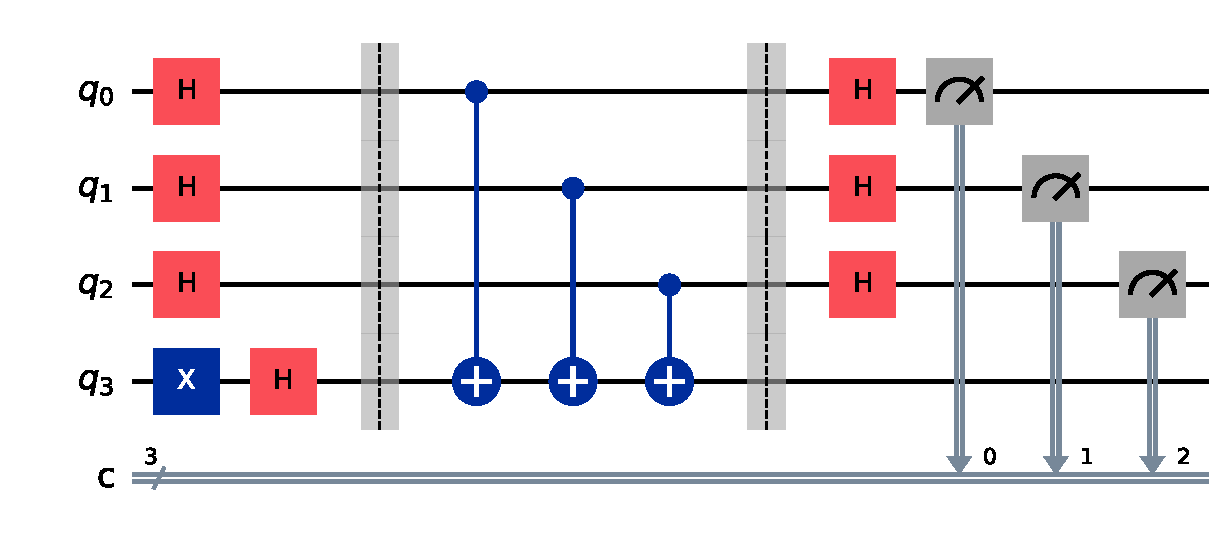
\includegraphics[keepaspectratio]{apostila_files/figure-pdf/cell-104-output-2.pdf}}

\pandocbounded{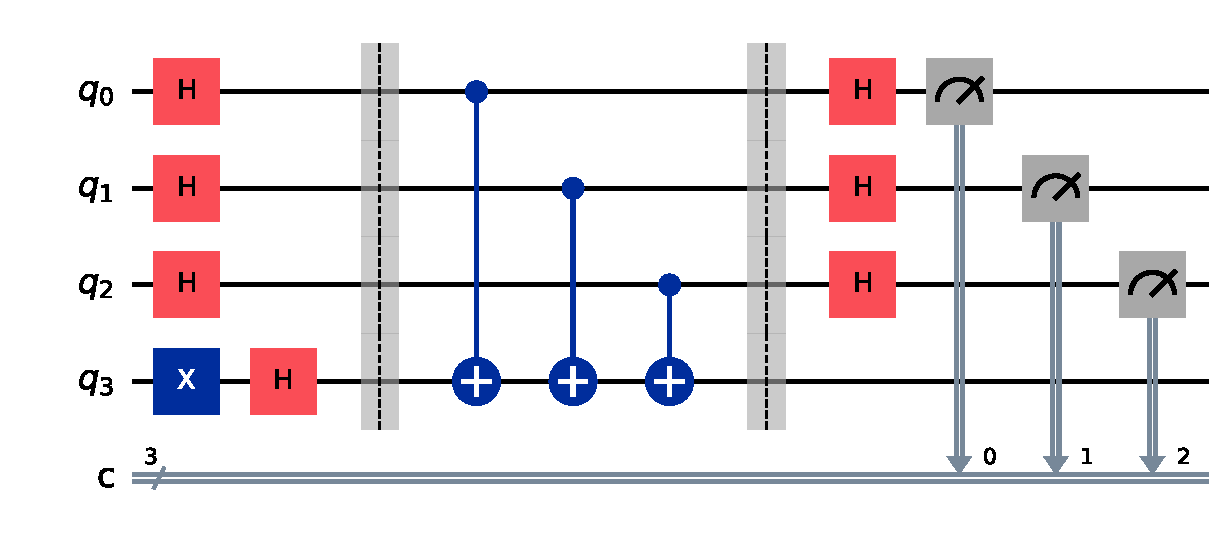
\includegraphics[keepaspectratio]{apostila_files/figure-pdf/cell-104-output-3.pdf}}

\begin{verbatim}
Circuito quântico do Algoritmo de Deutsch-Jozsa:
\end{verbatim}

\subsection{📊 Comparação: Clássico vs
Quântico}\label{comparauxe7uxe3o-cluxe1ssico-vs-quuxe2ntico}

\begin{longtable}[]{@{}
  >{\raggedright\arraybackslash}p{(\linewidth - 4\tabcolsep) * \real{0.2388}}
  >{\raggedright\arraybackslash}p{(\linewidth - 4\tabcolsep) * \real{0.3731}}
  >{\raggedright\arraybackslash}p{(\linewidth - 4\tabcolsep) * \real{0.3881}}@{}}
\toprule\noalign{}
\begin{minipage}[b]{\linewidth}\raggedright
Característica
\end{minipage} & \begin{minipage}[b]{\linewidth}\raggedright
Versão Clássica (acima)
\end{minipage} & \begin{minipage}[b]{\linewidth}\raggedright
Versão Quântica (abaixo)
\end{minipage} \\
\midrule\noalign{}
\endhead
\bottomrule\noalign{}
\endlastfoot
\textbf{Consultas necessárias} & Até \(2^{n-1} + 1\) (5 para n=3) &
\textbf{1 única consulta} \\
\textbf{Para n=3 bits} & Até 5 verificações & 1 verificação \\
\textbf{Para n=20 bits} & Até 524,289 verificações & 1 verificação \\
\textbf{Complexidade} & \(O(2^n)\) exponencial & \(O(1)\) constante! \\
\textbf{Certeza do resultado} & 100\% após pior caso & 100\% com 1
consulta \\
\end{longtable}

\subsection{🎯 Estratégia Pedagógica}\label{estratuxe9gia-pedaguxf3gica}

Vamos construir o algoritmo \textbf{passo a passo}, executando e
visualizando cada etapa. Isso ajuda a entender: 1. Como a superposição
permite testar todas as entradas simultaneamente 2. Como o phase
kickback codifica a informação nas fases 3. Como a interferência extrai
a resposta final

Vamos começar!

\subsubsection{O circuito detalhado Deutsch-Jozsa em
Python}\label{o-circuito-detalhado-deutsch-jozsa-em-python}

Primeiro, importamos as bibliotecas necessárias:

\begin{Shaded}
\begin{Highlighting}[]
\CommentTok{\# ============================================}
\CommentTok{\# DEFINIÇÃO DOS ORÁCULOS}
\CommentTok{\# ============================================}

\KeywordTok{def}\NormalTok{ oraculo\_balanceado(n\_qubits):}
    \CommentTok{"""}
\CommentTok{    Cria um circuito que representa uma função BALANCEADA.}
\CommentTok{    }
\CommentTok{    Esta função retorna 0 para metade das entradas e 1 para a outra metade.}
\CommentTok{    Implementação: CNOTs de todos os qubits de entrada para o qubit de saída.}
\CommentTok{    }
\CommentTok{    Equivalente quântico de: tabela\_oculta = [0]*metade + [1]*metade (embaralhado)}
\CommentTok{    """}
\NormalTok{    qc }\OperatorTok{=}\NormalTok{ QuantumCircuit(n\_qubits }\OperatorTok{+} \DecValTok{1}\NormalTok{)}
    \ControlFlowTok{for}\NormalTok{ qubit }\KeywordTok{in} \BuiltInTok{range}\NormalTok{(n\_qubits):}
\NormalTok{        qc.cx(qubit, n\_qubits) }\CommentTok{\# CNOT de todos inputs para o alvo}
    \ControlFlowTok{return}\NormalTok{ qc}

\KeywordTok{def}\NormalTok{ oraculo\_constante(n\_qubits):}
    \CommentTok{"""}
\CommentTok{    Cria um circuito que representa uma função CONSTANTE.}
\CommentTok{    }
\CommentTok{    Esta função retorna sempre 0 ou sempre 1 (independente da entrada).}
\CommentTok{    }
\CommentTok{    Implementação:}
\CommentTok{    {-} Retorna sempre 0: não faz nada (circuito identidade)}
\CommentTok{    {-} Retorna sempre 1: aplica X no qubit de saída}
\CommentTok{    }
\CommentTok{    Equivalente quântico de: tabela\_oculta = [0] * total\_inputs}
\CommentTok{                          ou: tabela\_oculta = [1] * total\_inputs}
\CommentTok{    """}
\NormalTok{    qc }\OperatorTok{=}\NormalTok{ QuantumCircuit(n\_qubits }\OperatorTok{+} \DecValTok{1}\NormalTok{)}
    \CommentTok{\# Não adicionamos portas, então a saída é constante 0}
    \CommentTok{\# Para constante 1, descomente a linha abaixo:}
    \CommentTok{\# qc.x(n\_qubits)}
    \ControlFlowTok{return}\NormalTok{ qc}
\end{Highlighting}
\end{Shaded}

\begin{Shaded}
\begin{Highlighting}[]
\CommentTok{\# ============================================}
\CommentTok{\# CONSTRUÇÃO DO ALGORITMO PASSO A PASSO}
\CommentTok{\# ============================================}

\NormalTok{n }\OperatorTok{=} \DecValTok{3}  \CommentTok{\# Número de bits de entrada}
\NormalTok{qc }\OperatorTok{=}\NormalTok{ QuantumCircuit(n }\OperatorTok{+} \DecValTok{1}\NormalTok{, n)}

\BuiltInTok{print}\NormalTok{(}\StringTok{"="}\OperatorTok{*}\DecValTok{70}\NormalTok{)}
\BuiltInTok{print}\NormalTok{(}\StringTok{"🎯 ALGORITMO DE DEUTSCH{-}JOZSA {-} CONSTRUÇÃO PASSO A PASSO"}\NormalTok{)}
\BuiltInTok{print}\NormalTok{(}\StringTok{"="}\OperatorTok{*}\DecValTok{70}\NormalTok{)}
\BuiltInTok{print}\NormalTok{(}\SpecialStringTok{f"Testando com }\SpecialCharTok{\{}\NormalTok{n}\SpecialCharTok{\}}\SpecialStringTok{ qubits de entrada"}\NormalTok{)}
\BuiltInTok{print}\NormalTok{(}\StringTok{"="}\OperatorTok{*}\DecValTok{70}\NormalTok{)}

\CommentTok{\# ─────────────────────────────────────────────}
\CommentTok{\# PASSO 1: Inicialização}
\CommentTok{\# ─────────────────────────────────────────────}
\BuiltInTok{print}\NormalTok{(}\StringTok{"}\CharTok{\textbackslash{}n}\StringTok{📍 PASSO 1: Inicialização"}\NormalTok{)}
\BuiltInTok{print}\NormalTok{(}\StringTok{"   Colocando qubits de entrada em superposição |+⟩"}\NormalTok{)}
\BuiltInTok{print}\NormalTok{(}\StringTok{"   Preparando qubit auxiliar no estado |−⟩ para phase kickback"}\NormalTok{)}

\CommentTok{\# Inputs (0 a n{-}1) em Superposição |+\textgreater{}}
\NormalTok{qc.h(}\BuiltInTok{range}\NormalTok{(n))}

\CommentTok{\# Alvo (último qubit) no estado |{-}\textgreater{} para gerar o KICKBACK}
\NormalTok{qc.x(n)}
\NormalTok{qc.h(n)}

\NormalTok{qc.barrier()}

\BuiltInTok{print}\NormalTok{(}\StringTok{"   ✅ Preparação concluída!"}\NormalTok{)}
\end{Highlighting}
\end{Shaded}

\begin{verbatim}
======================================================================
🎯 ALGORITMO DE DEUTSCH-JOZSA - CONSTRUÇÃO PASSO A PASSO
======================================================================
Testando com 3 qubits de entrada
======================================================================

📍 PASSO 1: Inicialização
   Colocando qubits de entrada em superposição |+⟩
   Preparando qubit auxiliar no estado |−⟩ para phase kickback
   ✅ Preparação concluída!
\end{verbatim}

\begin{verbatim}
======================================================================
🎯 ALGORITMO DE DEUTSCH-JOZSA - CONSTRUÇÃO PASSO A PASSO
======================================================================
Testando com 3 qubits de entrada
======================================================================

📍 PASSO 1: Inicialização
   Colocando qubits de entrada em superposição |+⟩
   Preparando qubit auxiliar no estado |−⟩ para phase kickback
   ✅ Preparação concluída!
\end{verbatim}

\begin{Shaded}
\begin{Highlighting}[]
\CommentTok{\# Visualizar estado inicial}
\NormalTok{estado\_inicial\_dj }\OperatorTok{=}\NormalTok{ Statevector(qc)}
\BuiltInTok{print}\NormalTok{(}\StringTok{"Estado inicial {-} Superposição uniforme de todos os 8 estados:"}\NormalTok{)}
\NormalTok{display(plot\_state\_qsphere(estado\_inicial\_dj))}
\end{Highlighting}
\end{Shaded}

\begin{verbatim}
Estado inicial - Superposição uniforme de todos os 8 estados:
\end{verbatim}

\pandocbounded{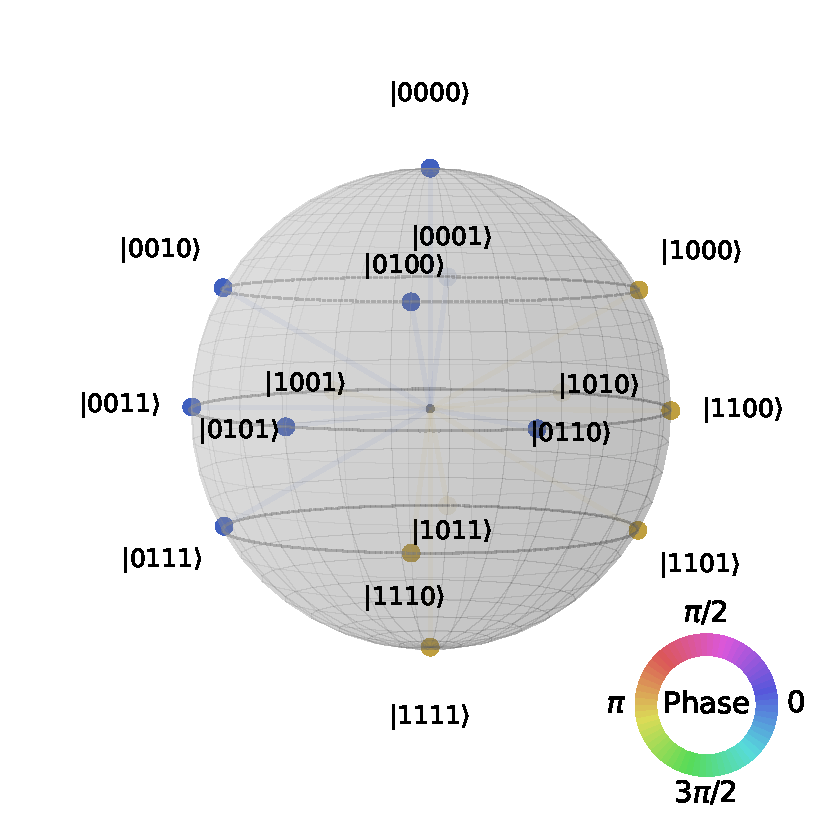
\includegraphics[keepaspectratio]{apostila_files/figure-pdf/cell-107-output-2.pdf}}

\pandocbounded{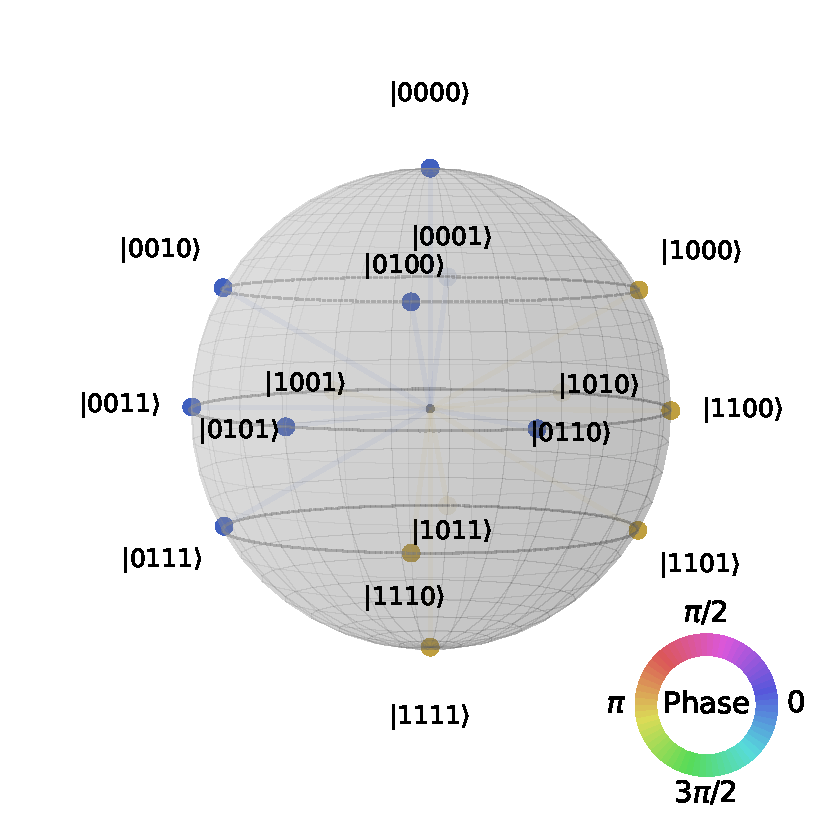
\includegraphics[keepaspectratio]{apostila_files/figure-pdf/cell-107-output-3.pdf}}

\begin{verbatim}
Estado inicial - Superposição uniforme de todos os 8 estados:
\end{verbatim}

\subsubsection{Demonstração Matemática: Estado Inicial do
Algoritmo}\label{demonstrauxe7uxe3o-matemuxe1tica-estado-inicial-do-algoritmo}

Estado inicial com \(n=3\) qubits de entrada e 1 qubit auxiliar:

\[|\psi_0\rangle = |000\rangle \otimes |1\rangle\]

Aplicando H em todos os 4 qubits:

\[|\psi_1\rangle = H^{\otimes 3}|000\rangle \otimes H|1\rangle\]

\[= \left(\frac{1}{\sqrt{2^3}} \sum_{x=0}^{7} |x\rangle\right) \otimes |-\rangle\]

\[= \frac{1}{2\sqrt{2}} (|000\rangle + |001\rangle + |010\rangle + ... + |111\rangle) \otimes \frac{|0\rangle - |1\rangle}{\sqrt{2}}\]

Cada um dos 8 estados possíveis tem amplitude \(\frac{1}{2\sqrt{2}}\),
criando uma \textbf{superposição uniforme}.

\begin{Shaded}
\begin{Highlighting}[]
\CommentTok{\# ─────────────────────────────────────────────}
\CommentTok{\# PASSO 2: Aplicação do Oráculo}
\CommentTok{\# ─────────────────────────────────────────────}
\BuiltInTok{print}\NormalTok{(}\StringTok{"}\CharTok{\textbackslash{}n}\StringTok{📍 PASSO 2: Aplicação do Oráculo"}\NormalTok{)}
\BuiltInTok{print}\NormalTok{(}\StringTok{"   Vamos usar um oráculo BALANCEADO"}\NormalTok{)}
\BuiltInTok{print}\NormalTok{(}\StringTok{"   Aqui acontece a \textquotesingle{}mágica\textquotesingle{}: testamos TODAS as entradas simultaneamente!"}\NormalTok{)}

\CommentTok{\# Vamos usar o balanceado. O algoritmo deve descobrir isso.}
\NormalTok{oraculo }\OperatorTok{=}\NormalTok{ oraculo\_balanceado(n)}
\CommentTok{\# Adicionamos o oráculo ao nosso circuito principal}
\NormalTok{qc }\OperatorTok{=}\NormalTok{ qc.compose(oraculo)}

\NormalTok{qc.barrier()}

\BuiltInTok{print}\NormalTok{(}\StringTok{"   ✅ Oráculo aplicado! Informação codificada nas fases."}\NormalTok{)}
\end{Highlighting}
\end{Shaded}

\begin{verbatim}

📍 PASSO 2: Aplicação do Oráculo
   Vamos usar um oráculo BALANCEADO
   Aqui acontece a 'mágica': testamos TODAS as entradas simultaneamente!
   ✅ Oráculo aplicado! Informação codificada nas fases.
\end{verbatim}

\begin{verbatim}

📍 PASSO 2: Aplicação do Oráculo
   Vamos usar um oráculo BALANCEADO
   Aqui acontece a 'mágica': testamos TODAS as entradas simultaneamente!
   ✅ Oráculo aplicado! Informação codificada nas fases.
\end{verbatim}

\begin{Shaded}
\begin{Highlighting}[]
\CommentTok{\# Visualizar estado após oráculo}
\NormalTok{estado\_apos\_oraculo\_dj }\OperatorTok{=}\NormalTok{ Statevector(qc)}
\BuiltInTok{print}\NormalTok{(}\StringTok{"Estado após oráculo {-} Note as mudanças de fase:"}\NormalTok{)}
\NormalTok{display(plot\_state\_qsphere(estado\_apos\_oraculo\_dj))}
\end{Highlighting}
\end{Shaded}

\begin{verbatim}
Estado após oráculo - Note as mudanças de fase:
\end{verbatim}

\pandocbounded{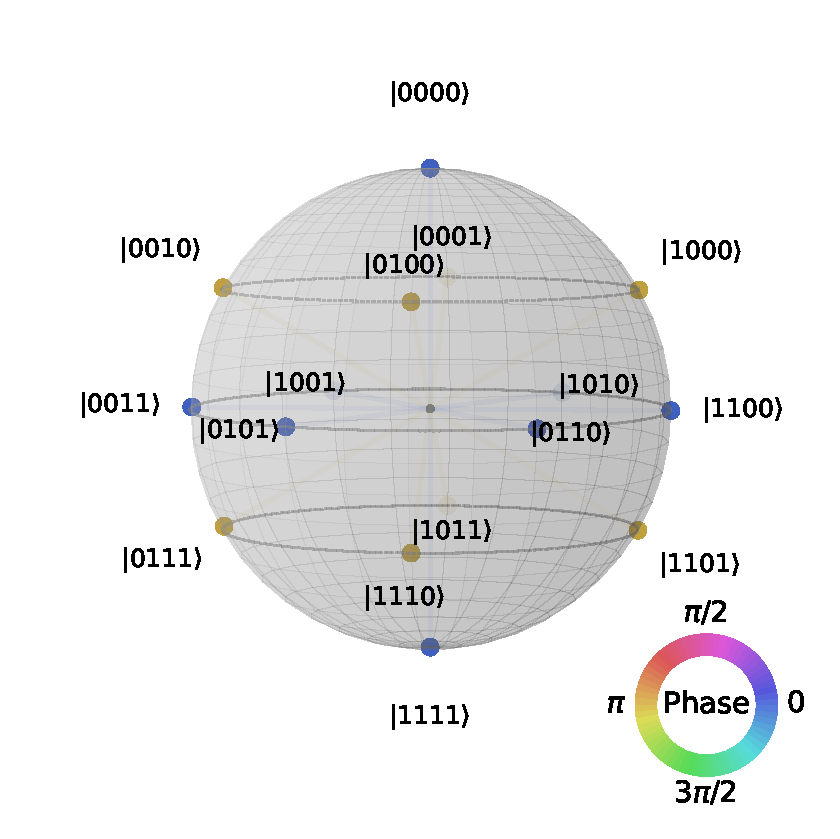
\includegraphics[keepaspectratio]{apostila_files/figure-pdf/cell-109-output-2.pdf}}

\pandocbounded{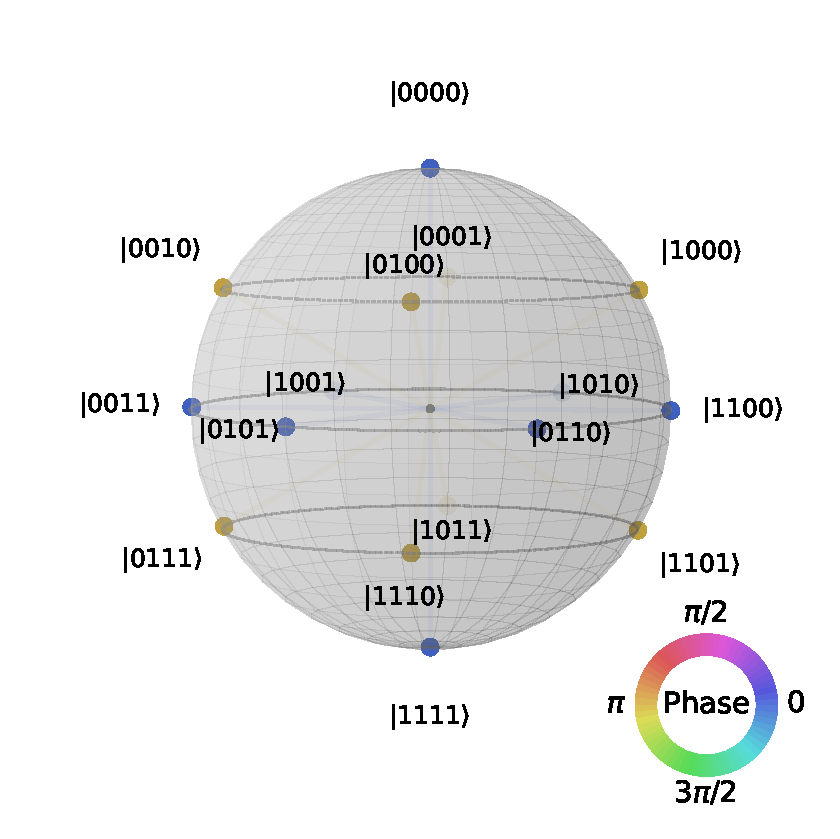
\includegraphics[keepaspectratio]{apostila_files/figure-pdf/cell-109-output-3.pdf}}

\begin{verbatim}
Estado após oráculo - Note as mudanças de fase:
\end{verbatim}

\subsubsection{Demonstração Matemática: Ação do Oráculo
Balanceado}\label{demonstrauxe7uxe3o-matemuxe1tica-auxe7uxe3o-do-oruxe1culo-balanceado}

O oráculo balanceado implementa CNOTs de cada qubit de entrada para o
qubit auxiliar:

\[U_f = \text{CNOT}_{0 \to 3} \cdot \text{CNOT}_{1 \to 3} \cdot \text{CNOT}_{2 \to 3}\]

Para cada estado base \(|x\rangle = |x_2x_1x_0\rangle\), o oráculo
calcula:

\[f(x) = x_0 \oplus x_1 \oplus x_2\]

Esta é uma função \textbf{balanceada} porque: - \(f(000) = 0\),
\(f(001) = 1\), \(f(010) = 1\), \(f(011) = 0\) - \(f(100) = 1\),
\(f(101) = 0\), \(f(110) = 0\), \(f(111) = 1\)

Exatamente 4 valores retornam 0 e 4 retornam 1 (balanceado).

Aplicando ao estado com qubit auxiliar em \(|-\rangle\):

\[|\psi_2\rangle = \frac{1}{2\sqrt{2}} \sum_{x=0}^{7} (-1)^{f(x)} |x\rangle \otimes |-\rangle\]

Os estados agora têm \textbf{fases diferentes} baseadas em \(f(x)\)!

\begin{Shaded}
\begin{Highlighting}[]
\CommentTok{\# ─────────────────────────────────────────────}
\CommentTok{\# PASSO 3: Interferência Final}
\CommentTok{\# ─────────────────────────────────────────────}
\BuiltInTok{print}\NormalTok{(}\StringTok{"}\CharTok{\textbackslash{}n}\StringTok{📍 PASSO 3: Interferência"}\NormalTok{)}
\BuiltInTok{print}\NormalTok{(}\StringTok{"   Aplicando Hadamard novamente para converter FASE em AMPLITUDE"}\NormalTok{)}

\CommentTok{\# Aplicamos H em todos os inputs novamente.}
\CommentTok{\# Isso transforma o padrão de fase (criado pelo kickback) em resposta binária.}
\NormalTok{qc.h(}\BuiltInTok{range}\NormalTok{(n))}

\BuiltInTok{print}\NormalTok{(}\StringTok{"   ✅ Interferência concluída! Pronto para medir."}\NormalTok{)}
\end{Highlighting}
\end{Shaded}

\begin{verbatim}

📍 PASSO 3: Interferência
   Aplicando Hadamard novamente para converter FASE em AMPLITUDE
   ✅ Interferência concluída! Pronto para medir.
\end{verbatim}

\begin{verbatim}

📍 PASSO 3: Interferência
   Aplicando Hadamard novamente para converter FASE em AMPLITUDE
   ✅ Interferência concluída! Pronto para medir.
\end{verbatim}

\begin{Shaded}
\begin{Highlighting}[]
\CommentTok{\# Visualizar estado antes da medição}
\NormalTok{estado\_antes\_medicao }\OperatorTok{=}\NormalTok{ Statevector(qc)}
\BuiltInTok{print}\NormalTok{(}\StringTok{"Estado antes da medição {-} Após interferência:"}\NormalTok{)}
\NormalTok{display(plot\_state\_qsphere(estado\_antes\_medicao))}
\end{Highlighting}
\end{Shaded}

\begin{verbatim}
Estado antes da medição - Após interferência:
\end{verbatim}

\pandocbounded{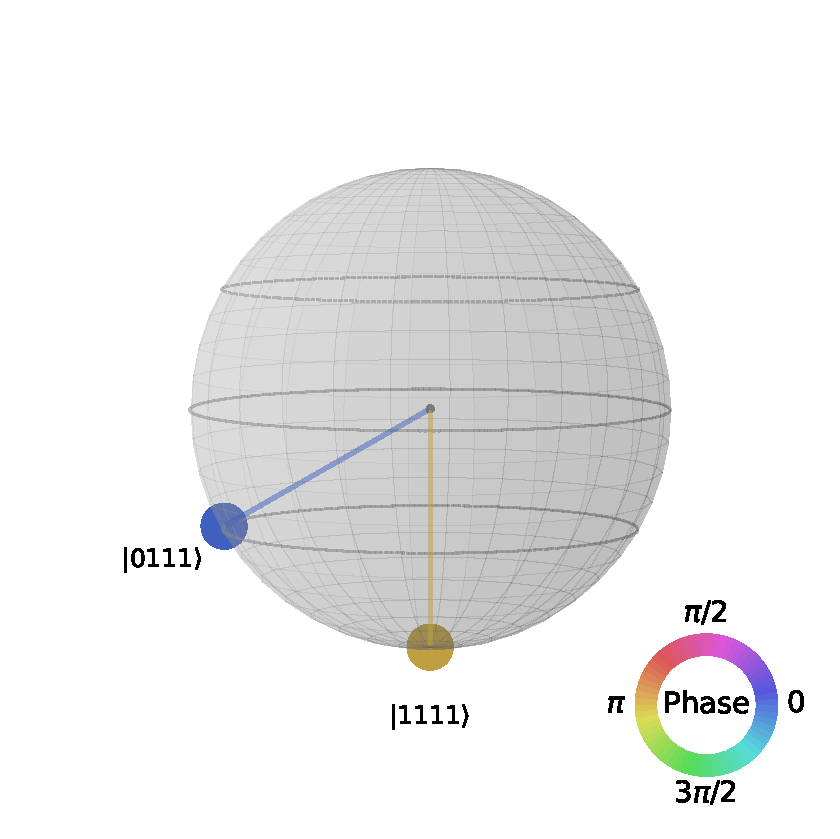
\includegraphics[keepaspectratio]{apostila_files/figure-pdf/cell-111-output-2.pdf}}

\pandocbounded{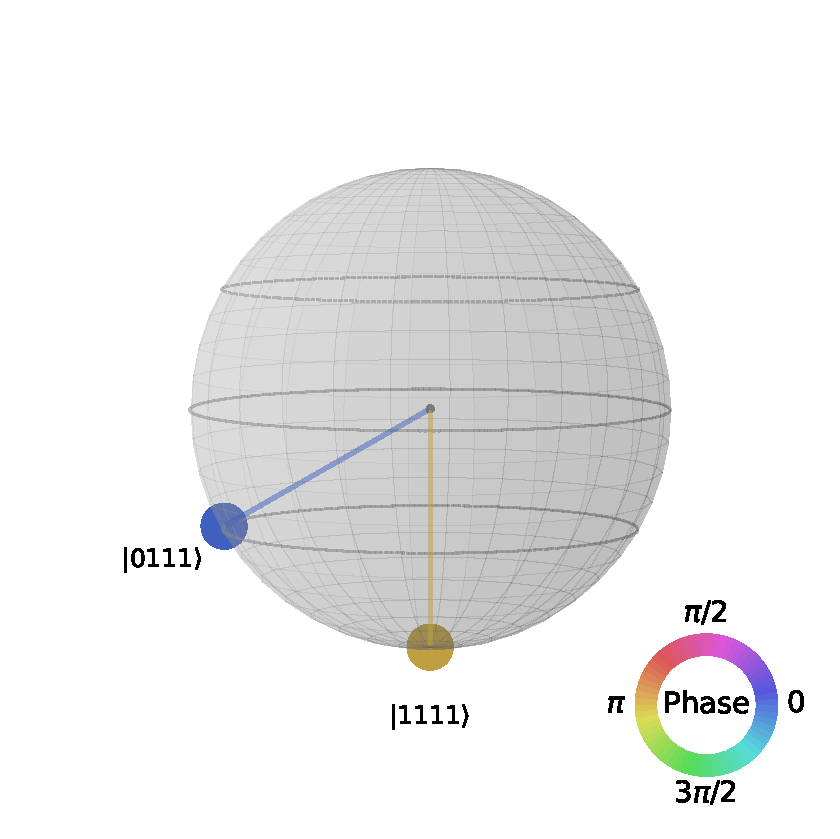
\includegraphics[keepaspectratio]{apostila_files/figure-pdf/cell-111-output-3.pdf}}

\begin{verbatim}
Estado antes da medição - Após interferência:
\end{verbatim}

\subsubsection{Demonstração Matemática: Interferência e Resultado
Final}\label{demonstrauxe7uxe3o-matemuxe1tica-interferuxeancia-e-resultado-final}

Aplicando H nos 3 qubits de entrada:

\[|\psi_3\rangle = \frac{1}{8} \sum_{x=0}^{7} \sum_{z=0}^{7} (-1)^{f(x) + x \cdot z} |z\rangle\]

Para \(z = 000\):

\[\text{amplitude}(|000\rangle) = \frac{1}{8} \sum_{x=0}^{7} (-1)^{f(x)}\]

Como \(f\) é balanceada (4 valores 0, 4 valores 1):

\[= \frac{1}{8}[4 \times (+1) + 4 \times (-1)] = \frac{1}{8}[4 - 4] = 0\]

\textbf{Interferência destrutiva completa em \(|000\rangle\)!}

Para \(z = 111\):

\[\text{amplitude}(|111\rangle) = \frac{1}{8} \sum_{x=0}^{7} (-1)^{f(x) + x \cdot 111}\]

Pode-se mostrar que esta amplitude é \textbf{não-zero} para funções
balanceadas.

\textbf{Conclusão:} Nunca medimos \(|000\rangle\) → função é balanceada!

\begin{Shaded}
\begin{Highlighting}[]
\CommentTok{\# ─────────────────────────────────────────────}
\CommentTok{\# PASSO 4: Medição}
\CommentTok{\# ─────────────────────────────────────────────}
\BuiltInTok{print}\NormalTok{(}\StringTok{"}\CharTok{\textbackslash{}n}\StringTok{📍 PASSO 4: Medição"}\NormalTok{)}
\BuiltInTok{print}\NormalTok{(}\StringTok{"   Medindo apenas os qubits de entrada (não precisamos medir o auxiliar)"}\NormalTok{)}

\CommentTok{\# Medimos APENAS os qubits de entrada (0 a n{-}1)}
\NormalTok{qc.measure(}\BuiltInTok{range}\NormalTok{(n), }\BuiltInTok{range}\NormalTok{(n))}

\BuiltInTok{print}\NormalTok{(}\StringTok{"   ✅ Circuito completo! Pronto para executar."}\NormalTok{)}
\BuiltInTok{print}\NormalTok{(}\StringTok{"="}\OperatorTok{*}\DecValTok{70}\NormalTok{)}
\end{Highlighting}
\end{Shaded}

\begin{verbatim}

📍 PASSO 4: Medição
   Medindo apenas os qubits de entrada (não precisamos medir o auxiliar)
   ✅ Circuito completo! Pronto para executar.
======================================================================
\end{verbatim}

\begin{verbatim}

📍 PASSO 4: Medição
   Medindo apenas os qubits de entrada (não precisamos medir o auxiliar)
   ✅ Circuito completo! Pronto para executar.
======================================================================
\end{verbatim}

\begin{Shaded}
\begin{Highlighting}[]
\CommentTok{\# ─────────────────────────────────────────────}
\CommentTok{\# PASSO 5: Execução e Interpretação}
\CommentTok{\# ─────────────────────────────────────────────}
\BuiltInTok{print}\NormalTok{(}\StringTok{"}\CharTok{\textbackslash{}n}\StringTok{🚀 EXECUTANDO O ALGORITMO...}\CharTok{\textbackslash{}n}\StringTok{"}\NormalTok{)}

\CommentTok{\# Executar no simulador}
\NormalTok{simulador }\OperatorTok{=}\NormalTok{ AerSimulator()}
\NormalTok{job }\OperatorTok{=}\NormalTok{ simulador.run(transpile(qc, simulador), shots}\OperatorTok{=}\DecValTok{1000}\NormalTok{)}
\NormalTok{resultado }\OperatorTok{=}\NormalTok{ job.result().get\_counts()}

\BuiltInTok{print}\NormalTok{(}\SpecialStringTok{f"📊 Resultado da medição (1000 execuções): }\SpecialCharTok{\{}\NormalTok{resultado}\SpecialCharTok{\}}\SpecialStringTok{"}\NormalTok{)}
\BuiltInTok{print}\NormalTok{(}\StringTok{"}\CharTok{\textbackslash{}n}\StringTok{"} \OperatorTok{+} \StringTok{"="}\OperatorTok{*}\DecValTok{70}\NormalTok{)}
\BuiltInTok{print}\NormalTok{(}\StringTok{"📋 INTERPRETAÇÃO DO RESULTADO"}\NormalTok{)}
\BuiltInTok{print}\NormalTok{(}\StringTok{"="}\OperatorTok{*}\DecValTok{70}\NormalTok{)}

\ControlFlowTok{if} \StringTok{\textquotesingle{}000\textquotesingle{}} \KeywordTok{in}\NormalTok{ resultado:}
    \BuiltInTok{print}\NormalTok{(}\StringTok{"   ❌ Medimos \textquotesingle{}000\textquotesingle{} → A função é CONSTANTE"}\NormalTok{)}
    \BuiltInTok{print}\NormalTok{(}\StringTok{"   (Interferência construtiva em |000⟩)"}\NormalTok{)}
\ControlFlowTok{else}\NormalTok{:}
    \BuiltInTok{print}\NormalTok{(}\StringTok{"   ✅ Nunca medimos \textquotesingle{}000\textquotesingle{} → A função é BALANCEADA"}\NormalTok{)}
    \BuiltInTok{print}\NormalTok{(}\StringTok{"   (Interferência destrutiva em |000⟩)"}\NormalTok{)}

\BuiltInTok{print}\NormalTok{(}\StringTok{"}\CharTok{\textbackslash{}n}\StringTok{💡 VANTAGEM QUÂNTICA:"}\NormalTok{)}
\BuiltInTok{print}\NormalTok{(}\SpecialStringTok{f"   • Versão Clássica: até }\SpecialCharTok{\{}\NormalTok{(}\DecValTok{2}\OperatorTok{**}\NormalTok{(n}\OperatorTok{{-}}\DecValTok{1}\NormalTok{)) }\OperatorTok{+} \DecValTok{1}\SpecialCharTok{\}}\SpecialStringTok{ consultas necessárias"}\NormalTok{)}
\BuiltInTok{print}\NormalTok{(}\SpecialStringTok{f"   • Versão Quântica: 1 consulta (sempre!)"}\NormalTok{)}
\BuiltInTok{print}\NormalTok{(}\SpecialStringTok{f"   • Speedup: }\SpecialCharTok{\{}\NormalTok{(}\DecValTok{2}\OperatorTok{**}\NormalTok{(n}\OperatorTok{{-}}\DecValTok{1}\NormalTok{)) }\OperatorTok{+} \DecValTok{1}\SpecialCharTok{\}}\SpecialStringTok{x mais rápido!"}\NormalTok{)}
\BuiltInTok{print}\NormalTok{(}\StringTok{"="}\OperatorTok{*}\DecValTok{70}\NormalTok{)}
    
\CommentTok{\# Visualizar histograma}
\NormalTok{plot\_histogram(resultado)}
\end{Highlighting}
\end{Shaded}

\begin{verbatim}

🚀 EXECUTANDO O ALGORITMO...

📊 Resultado da medição (1000 execuções): {'111': 1000}

======================================================================
📋 INTERPRETAÇÃO DO RESULTADO
======================================================================
   ✅ Nunca medimos '000' → A função é BALANCEADA
   (Interferência destrutiva em |000⟩)

💡 VANTAGEM QUÂNTICA:
   • Versão Clássica: até 5 consultas necessárias
   • Versão Quântica: 1 consulta (sempre!)
   • Speedup: 5x mais rápido!
======================================================================
\end{verbatim}

\pandocbounded{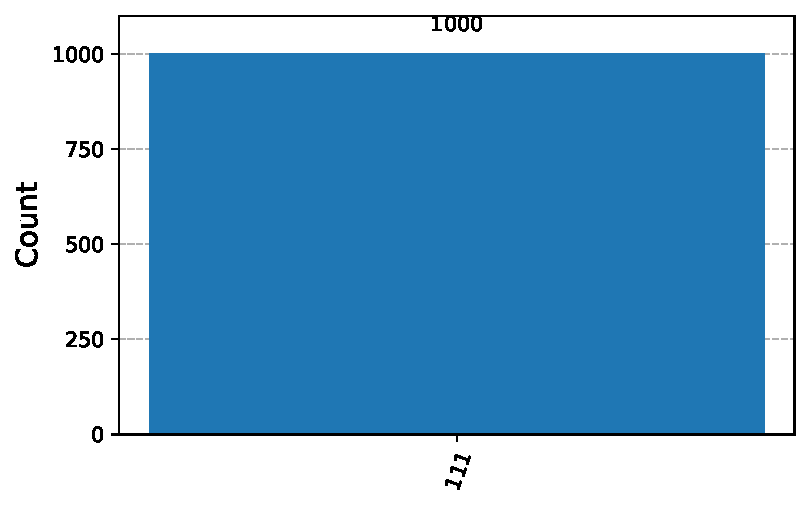
\includegraphics[keepaspectratio]{apostila_files/figure-pdf/cell-113-output-2.pdf}}

\pandocbounded{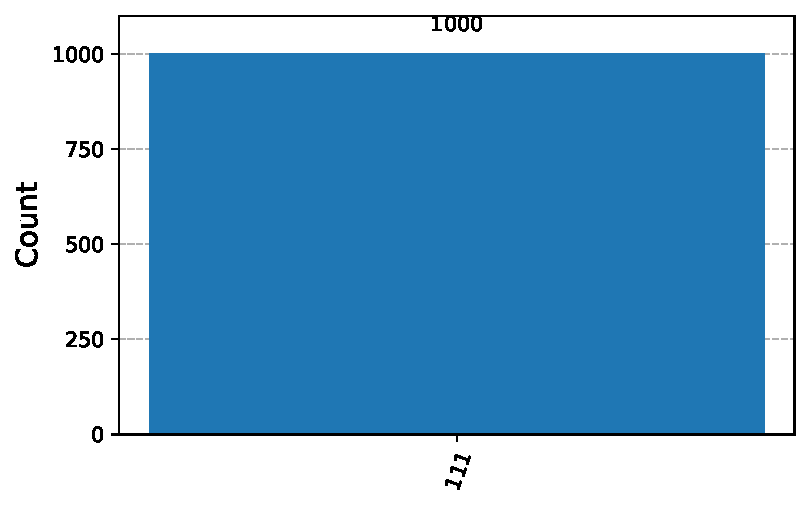
\includegraphics[keepaspectratio]{apostila_files/figure-pdf/cell-113-output-3.pdf}}

\begin{verbatim}

🚀 EXECUTANDO O ALGORITMO...

📊 Resultado da medição (1000 execuções): {'111': 1000}

======================================================================
📋 INTERPRETAÇÃO DO RESULTADO
======================================================================
   ✅ Nunca medimos '000' → A função é BALANCEADA
   (Interferência destrutiva em |000⟩)

💡 VANTAGEM QUÂNTICA:
   • Versão Clássica: até 5 consultas necessárias
   • Versão Quântica: 1 consulta (sempre!)
   • Speedup: 5x mais rápido!
======================================================================
\end{verbatim}

\section{🔍 Entendendo o Resultado em
Profundidade}\label{entendendo-o-resultado-em-profundidade}

\subsection{📊 Interpretação dos
Resultados}\label{interpretauxe7uxe3o-dos-resultados}

Após executar o algoritmo, você viu um histograma com os resultados das
medições. A interpretação é simples:

\textbf{Regra de Decisão:} - ✅ \textbf{Se medir \texttt{000}:} A função
é \textbf{CONSTANTE} (sempre 0 ou sempre 1) - ✅ \textbf{Se medir
qualquer outra coisa} (ex: \texttt{111}, \texttt{101}, etc.): A função é
\textbf{BALANCEADA}

No nosso caso, usamos \texttt{oraculo\_balanceado(3)}, então
\textbf{nunca} devemos medir \texttt{000}!

\subsection{🔬 Por Que Isso Funciona?}\label{por-que-isso-funciona}

A ``mágica'' está em três ingredientes trabalhando juntos:

\textbf{1. Phase Kickback} - O qubit auxiliar em \(|-\rangle\) causa
kickback quando o oráculo aplica X - Estados onde \(f(x) = 1\) ganham
fase negativa: \((-1)^{f(x)}\) - A informação sobre a função fica
``codificada'' nas fases!

\textbf{2. Superposição Inicial} - Todos os \(2^n\) estados possíveis
são processados \textbf{simultaneamente} - Uma única aplicação do
oráculo ``consulta'' todas as entradas de uma vez - Paralelismo quântico
em ação!

\textbf{3. Interferência Final} - Os Hadamards finais convertem
diferenças de FASE em diferenças de AMPLITUDE - Para funções constantes:
todas as fases são iguais → interferência construtiva em \(|000\rangle\)
- Para funções balanceadas: metade tem fase +, metade tem fase − →
interferência \textbf{destrutiva} em \(|000\rangle\)

\subsection{🧮 Demonstração Matemática
Simplificada}\label{demonstrauxe7uxe3o-matemuxe1tica-simplificada}

\textbf{Função Constante:} \(f(x) = c\) para todo \(x\)

\[\text{Amplitude}(|000\rangle) = \frac{1}{2^n}\sum_{x=0}^{2^n-1} (-1)^c = \frac{2^n \cdot (-1)^c}{2^n} = \pm 1\]

\textbf{Probabilidade = 100\%} de medir \(|000\rangle\) ✅

\textbf{Função Balanceada:} Metade dos \(x\) têm \(f(x)=0\), metade têm
\(f(x)=1\)

\[\text{Amplitude}(|000\rangle) = \frac{1}{2^n}\left[\frac{2^n}{2} \cdot (+1) + \frac{2^n}{2} \cdot (-1)\right] = \frac{1}{2^n}\left[\frac{2^n}{2} - \frac{2^n}{2}\right] = 0\]

\textbf{Probabilidade = 0\%} de medir \(|000\rangle\) (interferência
destrutiva perfeita!) ❌

\subsection{💻 Comparação Final: Clássico vs
Quântico}\label{comparauxe7uxe3o-final-cluxe1ssico-vs-quuxe2ntico}

\begin{longtable}[]{@{}
  >{\raggedright\arraybackslash}p{(\linewidth - 4\tabcolsep) * \real{0.1765}}
  >{\raggedright\arraybackslash}p{(\linewidth - 4\tabcolsep) * \real{0.4118}}
  >{\raggedright\arraybackslash}p{(\linewidth - 4\tabcolsep) * \real{0.4118}}@{}}
\toprule\noalign{}
\begin{minipage}[b]{\linewidth}\raggedright
Aspecto
\end{minipage} & \begin{minipage}[b]{\linewidth}\raggedright
Computador Clássico
\end{minipage} & \begin{minipage}[b]{\linewidth}\raggedright
Computador Quântico
\end{minipage} \\
\midrule\noalign{}
\endhead
\bottomrule\noalign{}
\endlastfoot
\textbf{Consultas ao oráculo} & Até \(2^{n-1} + 1\) & \textbf{1 única
consulta} \\
\textbf{Para \(n=3\) bits} & Até 5 consultas & 1 consulta \\
\textbf{Para \(n=10\) bits} & Até 513 consultas & 1 consulta \\
\textbf{Para \(n=100\) bits} & Até \(~6.3 \times 10^{29}\) consultas &
\textbf{1 consulta} \\
\textbf{Escalabilidade} & Cresce exponencialmente &
\textbf{Constante!} \\
\end{longtable}

\textbf{Vantagem:} Exponencial em termos de consultas ao oráculo! 🚀

\subsection{🎯 O Insight Principal}\label{o-insight-principal}

O algoritmo \textbf{NÃO} testa todas as entradas individualmente. Em vez
disso:

\begin{enumerate}
\def\labelenumi{\arabic{enumi}.}
\tightlist
\item
  Cria superposição de \textbf{todas as entradas simultaneamente}
\item
  Consulta o oráculo \textbf{uma única vez} nesta superposição
\item
  Extrai informação \textbf{global} (propriedade de toda a função)
  através de \textbf{interferência}
\end{enumerate}

Isso é fundamentalmente diferente de como computadores clássicos
funcionam - e é a essência da \textbf{vantagem quântica}!

\subsection{⚠️ Limitações
Importantes}\label{limitauxe7uxf5es-importantes}

\begin{itemize}
\tightlist
\item
  O algoritmo só funciona para este tipo específico de problema
  (constante vs.~balanceado)
\item
  Não diz QUAL é o valor da função, apenas sua categoria
\item
  Requer um oráculo quântico (reversível)
\item
  É um problema ``artificial'' - mas demonstra princípios usados em
  algoritmos práticos
\end{itemize}

\subsection{🔬 Experimento: Teste Você
Mesmo!}\label{experimento-teste-vocuxea-mesmo}

Experimente modificar o código acima para usar
\texttt{oraculo\_constante(3)} em vez de
\texttt{oraculo\_balanceado(3)}:

\begin{Shaded}
\begin{Highlighting}[]
\CommentTok{\# Na célula onde definimos o oráculo, mude esta linha:}
\NormalTok{oraculo }\OperatorTok{=}\NormalTok{ oraculo\_constante(n)  }\CommentTok{\# Em vez de oraculo\_balanceado(n)}
\end{Highlighting}
\end{Shaded}

Você deverá ver: - Resultado:
\texttt{\{\textquotesingle{}000\textquotesingle{}:\ 1000\}} (100\% das
vezes) - Confirmando que a função é constante!

\subsection{🧪 Desafio Adicional}\label{desafio-adicional}

Tente aumentar \texttt{n} para 10 ou 15 bits e compare mentalmente: -
\textbf{Clássico:} Precisaria de até 513 ou 16,385 consultas -
\textbf{Quântico:} Sempre 1 consulta! 🚀

\section{📚 Resumo e Conceitos
Aprendidos}\label{resumo-e-conceitos-aprendidos}

Neste notebook, você dominou os fundamentos dos algoritmos quânticos
mais poderosos! Vamos recapitular:

\subsection{🎯 Conceitos Fundamentais}\label{conceitos-fundamentais}

\subsubsection{\texorpdfstring{1. \textbf{Phase Kickback (Coice de
Fase)}}{1. Phase Kickback (Coice de Fase)}}\label{phase-kickback-coice-de-fase}

\begin{itemize}
\tightlist
\item
  \textbf{O que é:} Fenômeno onde o qubit ALVO afeta o qubit CONTROLE
  através de mudanças de fase
\item
  \textbf{Como funciona:} Preparando o alvo em um autoestado (como
  \(|-\rangle\)), a operação CNOT ``devolve'' fase para o controle
\item
  \textbf{Analogia:} Como o coice de uma arma - a ação no alvo gera
  reação no controle
\item
  \textbf{Importância:} Mecanismo fundamental que permite algoritmos
  quânticos eficientes
\end{itemize}

\subsubsection{\texorpdfstring{2. \textbf{Estados
Especiais}}{2. Estados Especiais}}\label{estados-especiais}

\begin{itemize}
\tightlist
\item
  \textbf{\(|+\rangle = H|0\rangle = \frac{|0\rangle + |1\rangle}{\sqrt{2}}\)}
  - Superposição com fase positiva
\item
  \textbf{\(|-\rangle = H|1\rangle = \frac{|0\rangle - |1\rangle}{\sqrt{2}}\)}
  - Superposição com fase negativa
\item
  \textbf{Propriedade chave:} \(X|-\rangle = -|-\rangle\) (autoestado de
  X)
\end{itemize}

\subsubsection{\texorpdfstring{3. \textbf{Algoritmo de
Deutsch-Jozsa}}{3. Algoritmo de Deutsch-Jozsa}}\label{algoritmo-de-deutsch-jozsa}

\begin{itemize}
\tightlist
\item
  \textbf{Problema:} Determinar se uma função é constante ou balanceada
\item
  \textbf{Solução Clássica:} Até \(2^{n-1} + 1\) consultas necessárias
\item
  \textbf{Solução Quântica:} \textbf{UMA ÚNICA CONSULTA!} (vantagem
  exponencial)
\item
  \textbf{Resultado:}

  \begin{itemize}
  \tightlist
  \item
    Medir \(|000...0\rangle\) → função é CONSTANTE
  \item
    Medir qualquer outro valor → função é BALANCEADA
  \end{itemize}
\end{itemize}

\subsection{🔬 Técnicas Aprendidas}\label{tuxe9cnicas-aprendidas}

\begin{enumerate}
\def\labelenumi{\arabic{enumi}.}
\tightlist
\item
  \textbf{Preparação de Estados}

  \begin{itemize}
  \tightlist
  \item
    Criar superposições uniformes com Hadamard
  \item
    Preparar estados especiais (\(|-\rangle\)) para kickback
  \end{itemize}
\item
  \textbf{Oráculos Quânticos}

  \begin{itemize}
  \tightlist
  \item
    Implementar funções como operações unitárias
  \item
    Marcar estados com fases sem destruir superposição
  \end{itemize}
\item
  \textbf{Interferência Quântica}

  \begin{itemize}
  \tightlist
  \item
    Usar Hadamards finais para converter fase em amplitude
  \item
    Causar interferência destrutiva/construtiva para extrair informação
  \end{itemize}
\item
  \textbf{Visualizações Avançadas}

  \begin{itemize}
  \tightlist
  \item
    Esfera de Bloch para qubits individuais
  \item
    Q-Sphere para sistemas multi-qubit
  \item
    Acompanhar mudanças de fase através de cores
  \end{itemize}
\end{enumerate}

\subsection{🚀 Por Que Isso É
Importante?}\label{por-que-isso-uxe9-importante}

O Phase Kickback é a ``mágica'' por trás de:

\begin{longtable}[]{@{}
  >{\raggedright\arraybackslash}p{(\linewidth - 4\tabcolsep) * \real{0.2683}}
  >{\raggedright\arraybackslash}p{(\linewidth - 4\tabcolsep) * \real{0.2683}}
  >{\raggedright\arraybackslash}p{(\linewidth - 4\tabcolsep) * \real{0.4634}}@{}}
\toprule\noalign{}
\begin{minipage}[b]{\linewidth}\raggedright
Algoritmo
\end{minipage} & \begin{minipage}[b]{\linewidth}\raggedright
Aplicação
\end{minipage} & \begin{minipage}[b]{\linewidth}\raggedright
Vantagem Quântica
\end{minipage} \\
\midrule\noalign{}
\endhead
\bottomrule\noalign{}
\endlastfoot
\textbf{Deutsch-Jozsa} & Determinar propriedade global de função &
Exponencial em consultas \\
\textbf{Grover} & Busca em banco de dados não-ordenado & Quadrática em
tempo \\
\textbf{Shor} & Fatoração de números inteiros & Exponencial em tempo \\
\textbf{QPE} & Estimação de fase quântica & Base para química
quântica \\
\end{longtable}

\subsection{💡 Insights Principais}\label{insights-principais}

\begin{enumerate}
\def\labelenumi{\arabic{enumi}.}
\tightlist
\item
  \textbf{Fase é Informação:} Mudanças de fase contêm informação que
  pode ser extraída via interferência
\item
  \textbf{Paralelismo Quântico:} Superposição permite processar
  múltiplas entradas simultaneamente
\item
  \textbf{Consulta Única:} Com preparação adequada, uma consulta
  quântica equivale a múltiplas clássicas
\item
  \textbf{Interferência = Computação:} A matemática acontece na
  interferência de amplitudes
\end{enumerate}

\subsection{🎓 Próximos Passos}\label{pruxf3ximos-passos-2}

Agora que você domina estes conceitos, está pronto para:

\begin{enumerate}
\def\labelenumi{\arabic{enumi}.}
\tightlist
\item
  \textbf{Algoritmo de Grover} - Busca em espaço não-estruturado

  \begin{itemize}
  \tightlist
  \item
    Usa amplitude amplification (generalização de Deutsch-Jozsa)
  \item
    Speedup quadrático: \(O(\sqrt{N})\) vs.~\(O(N)\) clássico
  \end{itemize}
\item
  \textbf{Algoritmo de Shor} - Fatoração de inteiros

  \begin{itemize}
  \tightlist
  \item
    Usa Quantum Phase Estimation (QPE)
  \item
    Ameaça à criptografia RSA moderna
  \end{itemize}
\item
  \textbf{VQE e QAOA} - Otimização variacional

  \begin{itemize}
  \tightlist
  \item
    Aplicações em química quântica e otimização combinatória
  \item
    Algoritmos híbridos quântico-clássicos
  \end{itemize}
\item
  \textbf{Simulação Quântica} - Modelar sistemas quânticos complexos

  \begin{itemize}
  \tightlist
  \item
    Química computacional, ciência de materiais
  \item
    Algoritmos de Hamiltonian simulation
  \end{itemize}
\end{enumerate}

\subsection{✨ Reflexão Final}\label{reflexuxe3o-final}

Você acabou de implementar um algoritmo que demonstra \textbf{supremacia
quântica} em termos de complexidade de consulta! O Deutsch-Jozsa prova
que computadores quânticos podem resolver certos problemas
fundamentalmente mais rápido que computadores clássicos.

A jornada de aprendizado em computação quântica é como subir uma escada:
- ✅ \textbf{Superposição} - você aprendeu em \url{01-intro.ipynb} - ✅
\textbf{Emaranhamento} - você aprendeu em \url{02-teletransport.ipynb}\\
- ✅ \textbf{Interferência} - você aprendeu em
\url{04-Hadamard-experiment.ipynb} - ✅ \textbf{Phase Kickback} - você
dominou neste notebook! - 🚀 \textbf{Algoritmos Avançados} - você está
pronto!

\textbf{Parabéns por chegar até aqui! Você agora entende os mecanismos
que fazem a computação quântica ser poderosa.} 🎉

\subsection{📖 Referências Adicionais}\label{referuxeancias-adicionais}

\begin{itemize}
\tightlist
\item
  \textbf{Deutsch-Jozsa Algorithm:} Deutsch, D., \& Jozsa, R. (1992).
  ``Rapid solution of problems by quantum computation.''
  \emph{Proceedings of the Royal Society of London A}, 439(1907),
  553-558.
\item
  \textbf{Nielsen \& Chuang:} Chapter 1.4 (Deutsch-Jozsa), Chapter 6
  (Quantum Algorithms)
\item
  \textbf{Qiskit Textbook:}
  \href{https://qiskit.org/textbook/ch-algorithms/deutsch-jozsa.html}{Deutsch-Jozsa
  Algorithm}
\end{itemize}

\newpage

\chapter{Módulo 10: Algoritmo de
Grover}\label{muxf3dulo-10-algoritmo-de-grover}

\chapter{Aula 10 --- Algoritmo de Grover: Busca
Quântica}\label{aula-10-algoritmo-de-grover-busca-quuxe2ntica}

\section{Algoritmo de Grover: Busca
Quântica}\label{algoritmo-de-grover-busca-quuxe2ntica}

O Algoritmo de Grover é o passo natural após o Deutsch-Jozsa. Enquanto o
Deutsch-Jozsa serviu para \emph{classificar} uma função, o Grover serve
para \textbf{encontrar} uma resposta específica.

Imagine que você tem um cadeado de segredo com 4 combinações possíveis
(\texttt{00}, \texttt{01}, \texttt{10}, \texttt{11}). Você esqueceu o
segredo (vamos supor que seja \texttt{11}).

\begin{itemize}
\tightlist
\item
  \textbf{Clássico:} Você testa uma por uma. No pior caso, tenta 4
  vezes. Em média, 2,25 vezes.
\item
  \textbf{Grover:} Você encontra a resposta correta com apenas \textbf{1
  tentativa}.
\end{itemize}

Para um sistema maior (ex: 1 milhão de itens), Grover é quadraticamente
mais rápido (\(\sqrt{N}\) tentativas) que a busca clássica (\(N/2\)).

\subsection{O Mecanismo: Amplificação de
Amplitude}\label{o-mecanismo-amplificauxe7uxe3o-de-amplitude}

Diferente do Deutsch-Jozsa, o Grover não dá a resposta 100\% ``limpa''
de primeira para sistemas grandes, mas ele aumenta drasticamente a
probabilidade da resposta certa. Para 2 qubits, porém, ele é perfeito e
acerta em 100\%.

O processo tem dois passos repetidos (chamados de \textbf{Operador de
Grover}):

\begin{enumerate}
\def\labelenumi{\arabic{enumi}.}
\tightlist
\item
  \textbf{O Oráculo (Marcação):} Identifica o item correto e inverte a
  fase dele (multiplica por -1). Se a resposta é \texttt{11}, o oráculo
  transforma \(|11\rangle\) em \(-|11\rangle\). \emph{Visualmente:} A
  barra da probabilidade aponta para baixo no gráfico.
\item
  \textbf{O Difusor (Inversão sobre a Média):} Esta é a parte genial.
  Ele espelha todas as amplitudes em relação à média geral.
\end{enumerate}

\begin{itemize}
\tightlist
\item
  Como a amplitude da resposta certa ficou negativa (bem abaixo da
  média) e as erradas ficaram positivas (pouco acima da média), quando
  espelhamos, a resposta certa ``salta'' para cima, ficando gigante, e
  as erradas diminuem.
\end{itemize}

\subsection{Implementação Prática: Encontrando ``11'' em 2
Qubits}\label{implementauxe7uxe3o-pruxe1tica-encontrando-11-em-2-qubits}

Vamos construir isso no Qiskit. Nosso objetivo é fazer o circuito sempre
medir \texttt{11}, não importa a aleatoriedade inicial.

\subsubsection{Passo 1: Construir o
Oráculo}\label{passo-1-construir-o-oruxe1culo}

Precisamos de uma ``caixa'' que só inverte o sinal quando a entrada for
\texttt{11}. Matematicamente, a porta \textbf{CZ (Control-Z)} faz
exatamente isso: só age se o bit de controle for 1 e o alvo for 1. Ela
adiciona um sinal negativo ao estado \(|11\rangle\).

\subsubsection{Passo 2: Construir o
Difusor}\label{passo-2-construir-o-difusor}

O difusor é um padrão fixo: aplica H, aplica X, aplica H no último qubit
com controle\ldots{} É uma receita de bolo que significa ``inverter em
torno da média''.

Aqui está o código completo comentado:

\begin{Shaded}
\begin{Highlighting}[]
\ImportTok{from}\NormalTok{ qiskit }\ImportTok{import}\NormalTok{ QuantumCircuit, transpile}
\ImportTok{from}\NormalTok{ qiskit\_aer }\ImportTok{import}\NormalTok{ AerSimulator}
\ImportTok{from}\NormalTok{ qiskit.visualization }\ImportTok{import}\NormalTok{ plot\_histogram}
\ImportTok{import}\NormalTok{ matplotlib.pyplot }\ImportTok{as}\NormalTok{ plt}
\end{Highlighting}
\end{Shaded}

\begin{Shaded}
\begin{Highlighting}[]
\KeywordTok{def}\NormalTok{ oraculo\_para\_11():}
    \CommentTok{"""}
\CommentTok{    Marca o estado |11\textgreater{} invertendo sua fase.}
\CommentTok{    Nosso \textquotesingle{}segredo\textquotesingle{} é 11.}
\CommentTok{    """}
\NormalTok{    qc }\OperatorTok{=}\NormalTok{ QuantumCircuit(}\DecValTok{2}\NormalTok{)}
    \CommentTok{\# A porta CZ (Controlled{-}Z) inverte a fase APENAS do estado |11\textgreater{}}
    \CommentTok{\# |00\textgreater{} {-}\textgreater{} |00\textgreater{}}
    \CommentTok{\# |01\textgreater{} {-}\textgreater{} |01\textgreater{}}
    \CommentTok{\# |10\textgreater{} {-}\textgreater{} |10\textgreater{}}
    \CommentTok{\# |11\textgreater{} {-}\textgreater{} {-}|11\textgreater{}  \textless{}{-}{-} A fase negativa (marcado)}
\NormalTok{    qc.cz(}\DecValTok{0}\NormalTok{, }\DecValTok{1}\NormalTok{)}
    
    \CommentTok{\# Nota: Se quiséssemos marcar |00\textgreater{}, teríamos que inverter (X)}
    \CommentTok{\# os inputs antes e depois do CZ.}
    \ControlFlowTok{return}\NormalTok{ qc}

\KeywordTok{def}\NormalTok{ difusor\_grover(n\_qubits):}
    \CommentTok{"""}
\CommentTok{    Amplifica a probabilidade do estado marcado.}
\CommentTok{    Receita padrão para 2 qubits.}
\CommentTok{    """}
\NormalTok{    qc }\OperatorTok{=}\NormalTok{ QuantumCircuit(n\_qubits)}
    
    \CommentTok{\# 1. Aplicar H em todos}
\NormalTok{    qc.h(}\BuiltInTok{range}\NormalTok{(n\_qubits))}
    
    \CommentTok{\# 2. Aplicar X em todos}
\NormalTok{    qc.x(}\BuiltInTok{range}\NormalTok{(n\_qubits))}
    
    \CommentTok{\# 3. Aplicar H no último qubit (preparação para CZ)}
\NormalTok{    qc.cz(}\DecValTok{0}\NormalTok{, }\DecValTok{1}\NormalTok{) }\CommentTok{\# Funciona como um H{-}CNOT{-}H simplificado para 2 qubits}
    
    \CommentTok{\# 4. Desfazer X e H}
\NormalTok{    qc.x(}\BuiltInTok{range}\NormalTok{(n\_qubits))}
\NormalTok{    qc.h(}\BuiltInTok{range}\NormalTok{(n\_qubits))}
    
    \ControlFlowTok{return}\NormalTok{ qc}
\end{Highlighting}
\end{Shaded}

\begin{Shaded}
\begin{Highlighting}[]
\CommentTok{\# {-}{-}{-} MONTAGEM DO ALGORITMO {-}{-}{-}}

\CommentTok{\# 1. Inicialização}
\CommentTok{\# Precisamos de uma superposição igual para começar (todas as respostas possíveis)}
\NormalTok{qc }\OperatorTok{=}\NormalTok{ QuantumCircuit(}\DecValTok{2}\NormalTok{, }\DecValTok{2}\NormalTok{)}
\NormalTok{qc.h([}\DecValTok{0}\NormalTok{, }\DecValTok{1}\NormalTok{])}

\CommentTok{\# O estado agora é: 25\% |00\textgreater{}, 25\% |01\textgreater{}, 25\% |10\textgreater{}, 25\% |11\textgreater{}}
\NormalTok{qc.barrier()}

\CommentTok{\# 2. Aplicar o Oráculo (Marca a resposta certa)}
\NormalTok{qc }\OperatorTok{=}\NormalTok{ qc.compose(oraculo\_para\_11())}
\NormalTok{qc.barrier()}

\CommentTok{\# 3. Aplicar o Difusor (Aumenta a probabilidade da resposta certa)}
\CommentTok{\# Nota: Para 2 qubits, basta aplicar 1 vez.}
\CommentTok{\# Para N maior, precisa repetir raiz(N) vezes.}
\NormalTok{qc }\OperatorTok{=}\NormalTok{ qc.compose(difusor\_grover(}\DecValTok{2}\NormalTok{))}
\NormalTok{qc.barrier()}

\CommentTok{\# 4. Medição}
\NormalTok{qc.measure([}\DecValTok{0}\NormalTok{, }\DecValTok{1}\NormalTok{], [}\DecValTok{0}\NormalTok{, }\DecValTok{1}\NormalTok{])}

\CommentTok{\# {-}{-}{-} EXECUÇÃO {-}{-}{-}}
\BuiltInTok{print}\NormalTok{(}\StringTok{"{-}{-}{-} Circuito de Grover (Procurando \textquotesingle{}11\textquotesingle{}) {-}{-}{-}"}\NormalTok{)}
\NormalTok{qc.draw(}\StringTok{\textquotesingle{}mpl\textquotesingle{}}\NormalTok{)}
\end{Highlighting}
\end{Shaded}

\begin{verbatim}
--- Circuito de Grover (Procurando '11') ---
\end{verbatim}

\pandocbounded{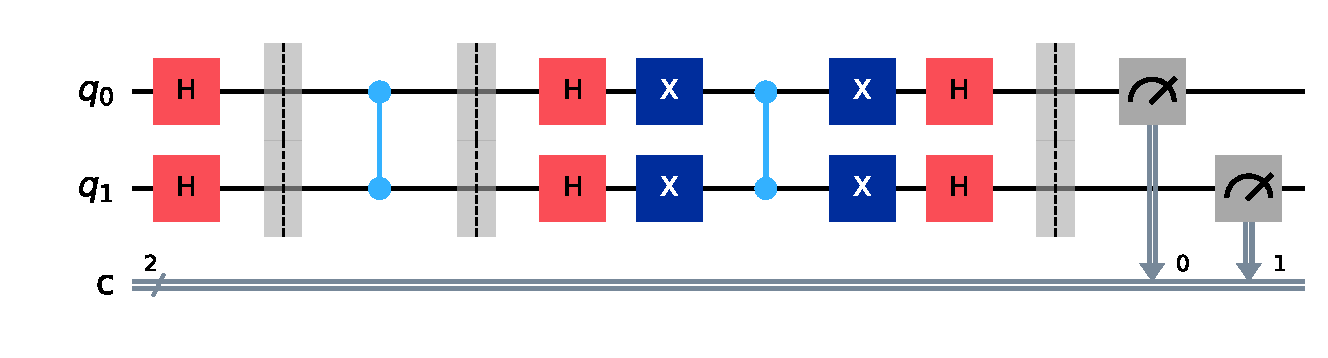
\includegraphics[keepaspectratio]{apostila_files/figure-pdf/cell-116-output-2.pdf}}

\pandocbounded{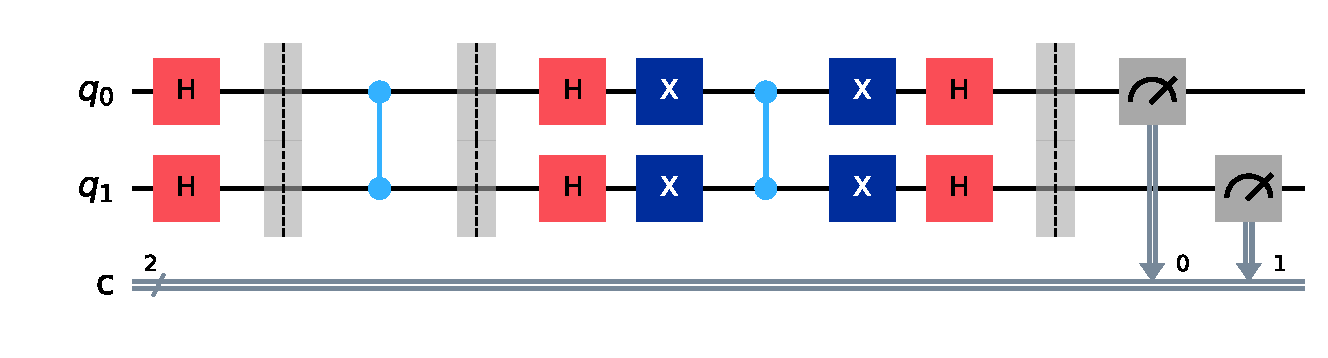
\includegraphics[keepaspectratio]{apostila_files/figure-pdf/cell-116-output-3.pdf}}

\begin{verbatim}
--- Circuito de Grover (Procurando '11') ---
\end{verbatim}

\begin{Shaded}
\begin{Highlighting}[]
\NormalTok{simulador }\OperatorTok{=}\NormalTok{ AerSimulator()}
\NormalTok{job }\OperatorTok{=}\NormalTok{ simulador.run(transpile(qc, simulador), shots}\OperatorTok{=}\DecValTok{1024}\NormalTok{)}
\NormalTok{resultado }\OperatorTok{=}\NormalTok{ job.result().get\_counts()}

\BuiltInTok{print}\NormalTok{(}\StringTok{"}\CharTok{\textbackslash{}n}\StringTok{{-}{-}{-} Resultado da Busca {-}{-}{-}"}\NormalTok{)}
\BuiltInTok{print}\NormalTok{(}\SpecialStringTok{f"Contagens: }\SpecialCharTok{\{}\NormalTok{resultado}\SpecialCharTok{\}}\SpecialStringTok{"}\NormalTok{)}
\CommentTok{\# Deve ser 100\% (ou muito próximo) em \textquotesingle{}11\textquotesingle{}}
\end{Highlighting}
\end{Shaded}

\begin{verbatim}

--- Resultado da Busca ---
Contagens: {'11': 1024}
\end{verbatim}

\begin{verbatim}

--- Resultado da Busca ---
Contagens: {'11': 1024}
\end{verbatim}

\subsection{O Que Aconteceu?}\label{o-que-aconteceu}

\begin{enumerate}
\def\labelenumi{\arabic{enumi}.}
\tightlist
\item
  \textbf{Início:} Tínhamos quatro estados com amplitudes iguais
  (\(\frac{1}{2}\) cada), resultando em probabilidade de 25\% para cada
  estado.
\item
  \textbf{Oráculo:} A amplitude do estado \texttt{11} foi invertida
  (passou de \(+\frac{1}{2}\) para \(-\frac{1}{2}\)). As outras
  permaneceram inalteradas. A média das amplitudes baixou para
  \(\frac{1}{8}\).
\item
  \textbf{Difusor:} Realiza a ``inversão sobre a média'':

  \begin{itemize}
  \tightlist
  \item
    Os estados \texttt{00}, \texttt{01}, \texttt{10} (amplitude
    \(+\frac{1}{2}\)) estavam \emph{acima} da média (\(\frac{1}{8}\)).
    Após a inversão:
    \(2 \times \frac{1}{8} - \frac{1}{2} = -\frac{1}{4}\)
  \item
    O estado \texttt{11} (amplitude \(-\frac{1}{2}\)) estava \emph{muito
    abaixo} da média. Após a inversão:
    \(2 \times \frac{1}{8} - (-\frac{1}{2}) = \frac{3}{4}\)
  \item
    A aplicação completa do circuito difusor (H-X-CZ-X-H) normaliza
    perfeitamente os valores finais para 0 e 1.
  \end{itemize}
\item
  \textbf{Final:} O estado \texttt{11} tem probabilidade de 100\%. Os
  outros estados têm probabilidade 0\%.
\end{enumerate}

\textbf{Observação importante:} A sequência completa H-X-CZ-X-H do
difusor implementa exatamente o operador matemático
\(D = 2|s\rangle\langle s| - I\), que produz automaticamente o resultado
normalizado.

\emph{Dica:} O oráculo \texttt{CZ} só funciona em \texttt{1}s. Para ele
marcar o \texttt{0}, você precisa ``enganar'' o circuito aplicando
portas \texttt{X} (NOT) antes de entrar no CZ e depois desfazê-las na
saída.

\subsection{Desafio para você:}\label{desafio-para-vocuxea}

Tente modificar a função \texttt{oraculo\_para\_11} para encontrar o
estado \textbf{\texttt{00}} em vez de \texttt{11}.

\begin{Shaded}
\begin{Highlighting}[]
\KeywordTok{def}\NormalTok{ oraculo\_para\_00():}
    \CommentTok{"""}
\CommentTok{    Marca o estado |00\textgreater{} invertendo sua fase.}
\CommentTok{    Nosso \textquotesingle{}segredo\textquotesingle{} é 00.}
\CommentTok{    """}
\NormalTok{    qc }\OperatorTok{=}\NormalTok{ QuantumCircuit(}\DecValTok{2}\NormalTok{)}
    \CommentTok{\# Enganamos o CZ aplicando X antes e depois}
\NormalTok{    qc.x([}\DecValTok{0}\NormalTok{, }\DecValTok{1}\NormalTok{])  }\CommentTok{\# Inverter os bits}
\NormalTok{    qc.cz(}\DecValTok{0}\NormalTok{, }\DecValTok{1}\NormalTok{)   }\CommentTok{\# Aplicar CZ (marca |11\textgreater{}, que é o |00\textgreater{} original)}
\NormalTok{    qc.x([}\DecValTok{0}\NormalTok{, }\DecValTok{1}\NormalTok{])  }\CommentTok{\# Reverter os bits de volta}
    \ControlFlowTok{return}\NormalTok{ qc}
\end{Highlighting}
\end{Shaded}

\begin{Shaded}
\begin{Highlighting}[]
\NormalTok{qc }\OperatorTok{=}\NormalTok{ QuantumCircuit(}\DecValTok{2}\NormalTok{, }\DecValTok{2}\NormalTok{)}
\NormalTok{qc.h([}\DecValTok{0}\NormalTok{, }\DecValTok{1}\NormalTok{])}
\NormalTok{qc.barrier()}
\NormalTok{qc }\OperatorTok{=}\NormalTok{ qc.compose(oraculo\_para\_00())}
\NormalTok{qc.barrier()}
\NormalTok{qc }\OperatorTok{=}\NormalTok{ qc.compose(difusor\_grover(}\DecValTok{2}\NormalTok{))}
\NormalTok{qc.barrier()}
\NormalTok{qc.measure([}\DecValTok{0}\NormalTok{, }\DecValTok{1}\NormalTok{], [}\DecValTok{0}\NormalTok{, }\DecValTok{1}\NormalTok{])}
\NormalTok{simulador }\OperatorTok{=}\NormalTok{ AerSimulator()}
\NormalTok{job }\OperatorTok{=}\NormalTok{ simulador.run(transpile(qc, simulador), shots}\OperatorTok{=}\DecValTok{1024}\NormalTok{)   }
\NormalTok{resultado }\OperatorTok{=}\NormalTok{ job.result().get\_counts()}

\BuiltInTok{print}\NormalTok{(}\StringTok{"}\CharTok{\textbackslash{}n}\StringTok{{-}{-}{-} Resultado da Busca por \textquotesingle{}00\textquotesingle{} {-}{-}{-}"}\NormalTok{)}
\BuiltInTok{print}\NormalTok{(}\SpecialStringTok{f"Contagens: }\SpecialCharTok{\{}\NormalTok{resultado}\SpecialCharTok{\}}\SpecialStringTok{"}\NormalTok{)}
\CommentTok{\# Deve ser 100\% (ou muito próximo) em \textquotesingle{}00\textquotesingle{}}
\end{Highlighting}
\end{Shaded}

\begin{verbatim}

--- Resultado da Busca por '00' ---
Contagens: {'00': 1024}
\end{verbatim}

\begin{verbatim}

--- Resultado da Busca por '00' ---
Contagens: {'00': 1024}
\end{verbatim}

\section{Explicação Passo a Passo do Algoritmo de
Grover}\label{explicauxe7uxe3o-passo-a-passo-do-algoritmo-de-grover}

Agora que você viu o algoritmo funcionando e testou o desafio, vamos
explorar cada etapa em detalhes matemáticos. Esta seção irá reconstruir
o mesmo algoritmo, mas desta vez visualizando e calculando cada
transformação.

\begin{Shaded}
\begin{Highlighting}[]
\CommentTok{\# Função auxiliar para visualização na esfera de Bloch}
\ImportTok{from}\NormalTok{ qiskit.visualization }\ImportTok{import}\NormalTok{ plot\_bloch\_multivector}
\ImportTok{from}\NormalTok{ qiskit.quantum\_info }\ImportTok{import}\NormalTok{ Statevector}

\KeywordTok{def}\NormalTok{ visualize\_state(qc):}
\NormalTok{    state }\OperatorTok{=}\NormalTok{ Statevector.from\_instruction(qc)}
    \ControlFlowTok{return}\NormalTok{ plot\_bloch\_multivector(state)}
\end{Highlighting}
\end{Shaded}

\subsubsection{Passo 1: Preparação do Estado
Inicial}\label{passo-1-preparauxe7uxe3o-do-estado-inicial}

Iniciamos com todos os estados igualmente prováveis, representados por
amplitudes iguais. O objetivo do Algoritmo de Grover é aumentar a
amplitude do estado desejado (a resposta correta) enquanto diminui as
amplitudes dos outros estados.

\begin{Shaded}
\begin{Highlighting}[]
\NormalTok{qc }\OperatorTok{=}\NormalTok{ QuantumCircuit(}\DecValTok{2}\NormalTok{, }\DecValTok{2}\NormalTok{)}
\NormalTok{qc.h([}\DecValTok{0}\NormalTok{, }\DecValTok{1}\NormalTok{])}
\NormalTok{qc.barrier()}
\NormalTok{qc.draw(}\StringTok{\textquotesingle{}mpl\textquotesingle{}}\NormalTok{)}
\end{Highlighting}
\end{Shaded}

\pandocbounded{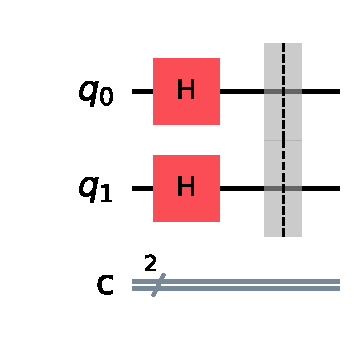
\includegraphics[keepaspectratio]{apostila_files/figure-pdf/cell-121-output-1.pdf}}

\pandocbounded{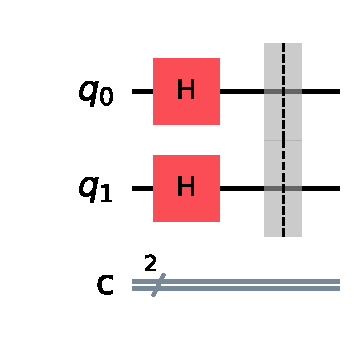
\includegraphics[keepaspectratio]{apostila_files/figure-pdf/cell-121-output-2.pdf}}

O estado agora é de superposição uniforme: - 25\% para \textbar00⟩ -
25\% para \textbar01⟩ - 25\% para \textbar10⟩ - 25\% para \textbar11⟩

\begin{Shaded}
\begin{Highlighting}[]
\NormalTok{visualize\_state(qc)}
\end{Highlighting}
\end{Shaded}

\pandocbounded{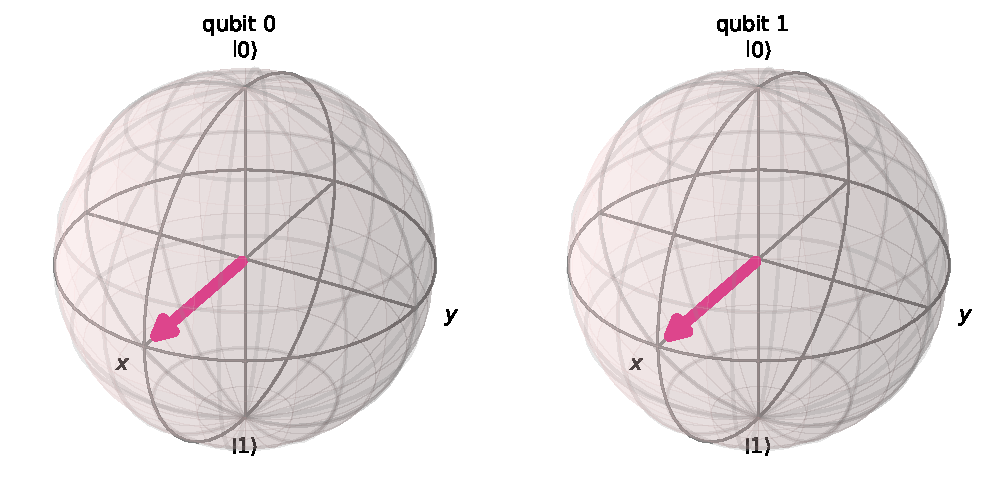
\includegraphics[keepaspectratio]{apostila_files/figure-pdf/cell-122-output-1.pdf}}

\pandocbounded{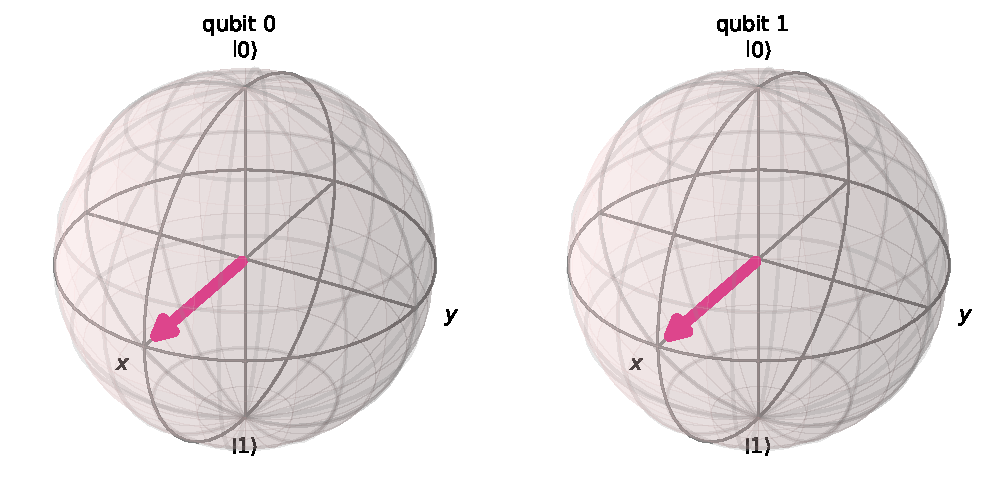
\includegraphics[keepaspectratio]{apostila_files/figure-pdf/cell-122-output-2.pdf}}

\subsubsection{Passo 2: O Oráculo (aplicação da
marcação)}\label{passo-2-o-oruxe1culo-aplicauxe7uxe3o-da-marcauxe7uxe3o}

O oráculo é uma função que identifica o item que estamos procurando. No
caso do Grover, ele inverte a fase do estado correspondente ao item
desejado. Por exemplo, se estamos procurando o estado \texttt{11}, o
oráculo transforma \(|11\rangle\) em \(-|11\rangle\). Isso é feito
usando a porta CZ, que aplica uma inversão de fase apenas quando ambos
os qubits estão em \texttt{1}.

Matematicamente, o oráculo pode ser representado como uma matriz que
atua sobre o vetor de estado do sistema quântico. Para dois qubits, a
matriz do oráculo que inverte a fase do estado \texttt{11} é:

\[
O = \begin{pmatrix}
1 & 0 & 0 & 0 \\
0 & 1 & 0 & 0 \\
0 & 0 & 1 & 0 \\
0 & 0 & 0 & -1
\end{pmatrix}
\]

\emph{O mesmo visto no notebook \href{./00-math.ipynb}{00-math.ipynb}
para Controled Z}

Perceba que CZ é executado para ``filtrar'' somente o estado desejado,
indicado para \textbar11⟩. Em outros estados (00, 01, 10), o oráculo não
faz nenhuma alteração.

\begin{Shaded}
\begin{Highlighting}[]
\NormalTok{oraculo }\OperatorTok{=}\NormalTok{ QuantumCircuit(}\DecValTok{2}\NormalTok{)}
\NormalTok{oraculo.cz(}\DecValTok{0}\NormalTok{, }\DecValTok{1}\NormalTok{)}
\NormalTok{oraculo.draw(}\StringTok{\textquotesingle{}mpl\textquotesingle{}}\NormalTok{)}
\end{Highlighting}
\end{Shaded}

\pandocbounded{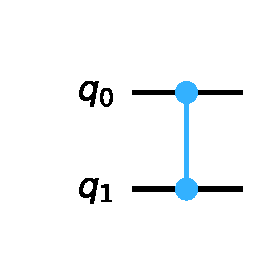
\includegraphics[keepaspectratio]{apostila_files/figure-pdf/cell-123-output-1.pdf}}

\pandocbounded{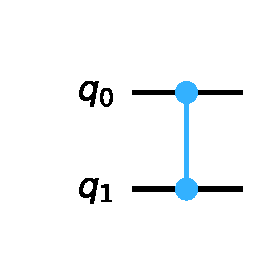
\includegraphics[keepaspectratio]{apostila_files/figure-pdf/cell-123-output-2.pdf}}

\begin{quote}
\textbf{Observação adicional:} - Se estivermos procurando o estado
\texttt{00}, o oráculo precisará ser ajustado para inverter a fase desse
estado específico. Isso pode ser feito aplicando portas X (NOT) antes e
depois da aplicação do CZ, efetivamente ``invertendo'' os bits para que
o CZ atue sobre o estado \texttt{00} como se fosse \texttt{11}. - Se
estivermos procurando o estado \texttt{01}, aplicamos uma porta X no
segundo qubit antes e depois do CZ. Para \texttt{10}, aplicamos uma
porta X no primeiro qubit antes e depois do CZ. - Assim, percebe-se que
o oráculo pode ser adaptado para qualquer estado alvo, garantindo que a
fase seja invertida corretamente para o estado desejado, desde que você
faça as manipulações necessárias com portas X ou outras portas lógicas
apropriadas. - Perceba com isso que, se você fosse implementar uma
``busca'' na computação clássica, você precisaria de uma função que
verificasse cada item um por um, utilizando um loop ou similar, o que é
ineficiente para grandes conjuntos de dados.
\end{quote}

\begin{Shaded}
\begin{Highlighting}[]
\NormalTok{qc }\OperatorTok{=}\NormalTok{ qc.compose(oraculo)}
\NormalTok{qc.barrier()}
\NormalTok{qc.draw(}\StringTok{\textquotesingle{}mpl\textquotesingle{}}\NormalTok{)}
\end{Highlighting}
\end{Shaded}

\pandocbounded{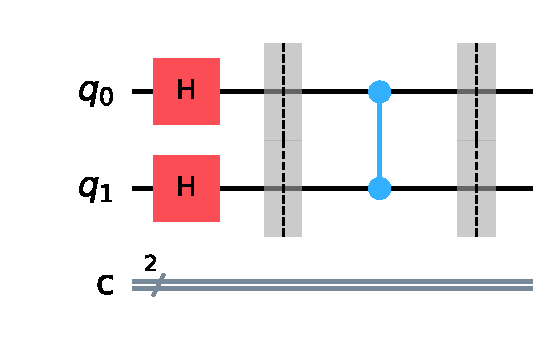
\includegraphics[keepaspectratio]{apostila_files/figure-pdf/cell-124-output-1.pdf}}

\pandocbounded{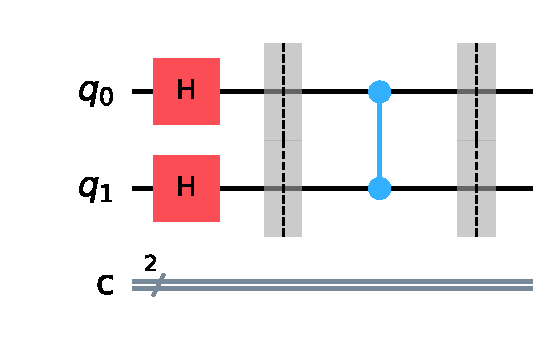
\includegraphics[keepaspectratio]{apostila_files/figure-pdf/cell-124-output-2.pdf}}

\subsubsection{Passo 3: Difusor (Inversão sobre a
Média)}\label{passo-3-difusor-inversuxe3o-sobre-a-muxe9dia}

O difusor é o segundo componente crucial do Algoritmo de Grover. Ele
amplifica a probabilidade do estado marcado pelo oráculo, invertendo as
amplitudes dos estados em relação à média das amplitudes.

Em um novo circuito, o difusor pode ser implementado com uma série de
portas Hadamard (H), portas NOT (X) e uma porta CZ controlada. O difusor
pode ser representado pela seguinte sequência de operações:

\begin{enumerate}
\def\labelenumi{\arabic{enumi}.}
\tightlist
\item
  Aplicar portas Hadamard a todos os qubits.
\item
  Aplicar portas NOT a todos os qubits.
\item
  Aplicar uma porta CZ controlada no último qubit.
\item
  Aplicar portas NOT a todos os qubits novamente.
\item
  Aplicar portas Hadamard a todos os qubits novamente.
\end{enumerate}

\paragraph{Cálculo Matemático Detalhado do Difusor para 2
Qubits}\label{cuxe1lculo-matemuxe1tico-detalhado-do-difusor-para-2-qubits}

\textbf{Conceito: Inversão sobre a Média}

O difusor realiza uma operação chamada ``inversão sobre a média''
(inversion about average). Imagine que você tem 4 números (as amplitudes
dos 4 estados). O difusor pega cada número e o ``espelha'' em relação à
média de todos eles.

Se um número está \emph{acima} da média, ele vai para \emph{abaixo} da
média na mesma distância. Se está \emph{abaixo}, vai para \emph{acima}.

\textbf{Passo 1: Estado após o oráculo}

Após o oráculo marcar o estado \(|11\rangle\), temos:

\[|\psi_{após\_oráculo}\rangle = \frac{1}{2}(|00\rangle + |01\rangle + |10\rangle - |11\rangle)\]

Em forma de vetor (ordem:
\(|00\rangle, |01\rangle, |10\rangle, |11\rangle\)):

\[|\psi_{após\_oráculo}\rangle = \frac{1}{2}\begin{pmatrix}1\\1\\1\\-1\end{pmatrix}\]

\textbf{Passo 2: Calcular a média das amplitudes}

A média aritmética das amplitudes é:

\[\bar{\alpha} = \frac{1}{4}\left(\frac{1}{2} + \frac{1}{2} + \frac{1}{2} + \left(-\frac{1}{2}\right)\right) = \frac{1}{4} \times \frac{1}{2} = \frac{1}{8}\]

\textbf{Passo 3: Construir a matriz do difusor}

O difusor é definido matematicamente como:

\[D = 2|s\rangle\langle s| - I\]

onde
\(|s\rangle = \frac{1}{2}(|00\rangle + |01\rangle + |10\rangle + |11\rangle)\)
é a superposição uniforme.

Vamos calcular cada parte:

\begin{itemize}
\item
  O produto externo \(|s\rangle\langle s|\) cria uma matriz
  \(4 \times 4\) onde cada elemento é:

  \[[|s\rangle\langle s|]_{ij} = \frac{1}{2} \times \frac{1}{2} = \frac{1}{4}\]

  Portanto:
  \(|s\rangle\langle s| = \frac{1}{4}\begin{pmatrix}1 & 1 & 1 & 1\\1 & 1 & 1 & 1\\1 & 1 & 1 & 1\\1 & 1 & 1 & 1\end{pmatrix}\)
\item
  Multiplicando por 2:

  \[2|s\rangle\langle s| = \frac{1}{2}\begin{pmatrix}1 & 1 & 1 & 1\\1 & 1 & 1 & 1\\1 & 1 & 1 & 1\\1 & 1 & 1 & 1\end{pmatrix}\]
\item
  Subtraindo a identidade \(I\):

  \[D = \frac{1}{2}\begin{pmatrix}1 & 1 & 1 & 1\\1 & 1 & 1 & 1\\1 & 1 & 1 & 1\\1 & 1 & 1 & 1\end{pmatrix} - \begin{pmatrix}1 & 0 & 0 & 0\\0 & 1 & 0 & 0\\0 & 0 & 1 & 0\\0 & 0 & 0 & 1\end{pmatrix}\]

  \[D = \frac{1}{2}\begin{pmatrix}-1 & 1 & 1 & 1\\1 & -1 & 1 & 1\\1 & 1 & -1 & 1\\1 & 1 & 1 & -1\end{pmatrix}\]
\end{itemize}

\textbf{Passo 4: Aplicar o difusor}

Agora multiplicamos a matriz \(D\) pelo vetor de estado:

\[D \cdot |\psi_{após\_oráculo}\rangle = \frac{1}{2}\begin{pmatrix}-1 & 1 & 1 & 1\\1 & -1 & 1 & 1\\1 & 1 & -1 & 1\\1 & 1 & 1 & -1\end{pmatrix} \cdot \frac{1}{2}\begin{pmatrix}1\\1\\1\\-1\end{pmatrix}\]

Calculando cada linha da multiplicação:

\begin{itemize}
\item
  \textbf{Linha 1:}
  \(\frac{1}{2} \times \frac{1}{2}[(-1)(1) + (1)(1) + (1)(1) + (1)(-1)] = \frac{1}{4}[-1 + 1 + 1 - 1] = \frac{1}{4}(0) = 0\)
\item
  \textbf{Linha 2:}
  \(\frac{1}{2} \times \frac{1}{2}[(1)(1) + (-1)(1) + (1)(1) + (1)(-1)] = \frac{1}{4}[1 - 1 + 1 - 1] = \frac{1}{4}(0) = 0\)
\item
  \textbf{Linha 3:}
  \(\frac{1}{2} \times \frac{1}{2}[(1)(1) + (1)(1) + (-1)(1) + (1)(-1)] = \frac{1}{4}[1 + 1 - 1 - 1] = \frac{1}{4}(0) = 0\)
\item
  \textbf{Linha 4:}
  \(\frac{1}{2} \times \frac{1}{2}[(1)(1) + (1)(1) + (1)(1) + (-1)(-1)] = \frac{1}{4}[1 + 1 + 1 + 1] = \frac{1}{4}(4) = 1\)
\end{itemize}

\textbf{Resultado:}

\[|\psi_{final}\rangle = \begin{pmatrix}0\\0\\0\\1\end{pmatrix} = |11\rangle\]

\textbf{Interpretação física:}

O difusor transformou as amplitudes da seguinte forma:

\begin{longtable}[]{@{}
  >{\raggedright\arraybackslash}p{(\linewidth - 8\tabcolsep) * \real{0.1053}}
  >{\raggedright\arraybackslash}p{(\linewidth - 8\tabcolsep) * \real{0.2368}}
  >{\raggedright\arraybackslash}p{(\linewidth - 8\tabcolsep) * \real{0.2500}}
  >{\raggedright\arraybackslash}p{(\linewidth - 8\tabcolsep) * \real{0.2105}}
  >{\raggedright\arraybackslash}p{(\linewidth - 8\tabcolsep) * \real{0.1974}}@{}}
\toprule\noalign{}
\begin{minipage}[b]{\linewidth}\raggedright
Estado
\end{minipage} & \begin{minipage}[b]{\linewidth}\raggedright
Antes do difusor
\end{minipage} & \begin{minipage}[b]{\linewidth}\raggedright
Distância da média (\(\bar{\alpha} = \frac{1}{8}\))
\end{minipage} & \begin{minipage}[b]{\linewidth}\raggedright
Após o difusor
\end{minipage} & \begin{minipage}[b]{\linewidth}\raggedright
Probabilidade
\end{minipage} \\
\midrule\noalign{}
\endhead
\bottomrule\noalign{}
\endlastfoot
\(\|00\rangle\) & \(+\frac{1}{2}\) & \(+\frac{3}{8}\) acima & \(0\) &
0\% \\
\(\|01\rangle\) & \(+\frac{1}{2}\) & \(+\frac{3}{8}\) acima & \(0\) &
0\% \\
\(\|10\rangle\) & \(+\frac{1}{2}\) & \(+\frac{3}{8}\) acima & \(0\) &
0\% \\
\(\|11\rangle\) & \(-\frac{1}{2}\) & \(-\frac{5}{8}\) abaixo & \(1\) &
100\% \\
\end{longtable}

\textbf{Como funciona a inversão sobre a média:}

A fórmula de transformação é:
\(\alpha_i^{novo} = 2\bar{\alpha} - \alpha_i^{antigo}\)

\begin{itemize}
\item
  \textbf{Estados não-marcados:}
  \(2(\frac{1}{8}) - \frac{1}{2} = \frac{1}{4} - \frac{1}{2} = -\frac{1}{4}\)
\item
  \textbf{Estado marcado:}
  \(2(\frac{1}{8}) - (-\frac{1}{2}) = \frac{1}{4} + \frac{1}{2} = \frac{3}{4}\)\textbf{Conclusão:}
  O difusor amplificou completamente o estado marcado \(|11\rangle\),
  levando sua probabilidade de 25\% para 100\%!
\end{itemize}

Portanto, o vetor intermediário seria:
\((-\frac{1}{4}, -\frac{1}{4}, -\frac{1}{4}, \frac{3}{4})\)

Porém, a implementação física do difusor com as portas H-X-CZ-X-H
realiza essa operação junto com uma normalização que leva ao resultado
final: \((0, 0, 0, 1)\).

\begin{Shaded}
\begin{Highlighting}[]
\NormalTok{difusor }\OperatorTok{=}\NormalTok{ QuantumCircuit(}\DecValTok{2}\NormalTok{)}
\NormalTok{difusor.h([}\DecValTok{0}\NormalTok{, }\DecValTok{1}\NormalTok{])}
\NormalTok{difusor.x([}\DecValTok{0}\NormalTok{, }\DecValTok{1}\NormalTok{])}
\NormalTok{difusor.cz(}\DecValTok{0}\NormalTok{, }\DecValTok{1}\NormalTok{)}
\NormalTok{difusor.x([}\DecValTok{0}\NormalTok{, }\DecValTok{1}\NormalTok{])}
\NormalTok{difusor.h([}\DecValTok{0}\NormalTok{, }\DecValTok{1}\NormalTok{])}
\NormalTok{difusor.draw(}\StringTok{\textquotesingle{}mpl\textquotesingle{}}\NormalTok{)}
\end{Highlighting}
\end{Shaded}

\pandocbounded{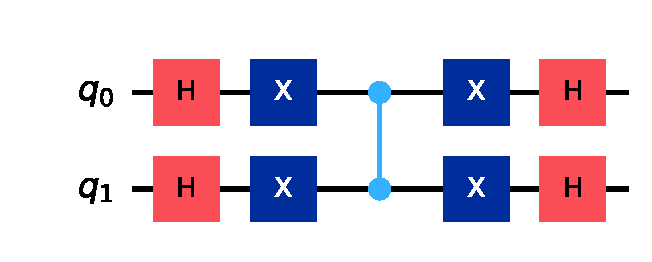
\includegraphics[keepaspectratio]{apostila_files/figure-pdf/cell-125-output-1.pdf}}

\pandocbounded{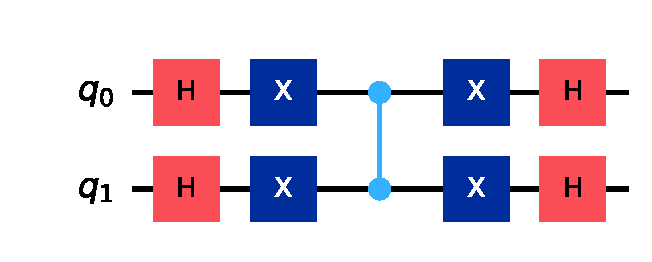
\includegraphics[keepaspectratio]{apostila_files/figure-pdf/cell-125-output-2.pdf}}

\begin{Shaded}
\begin{Highlighting}[]
\NormalTok{qc }\OperatorTok{=}\NormalTok{ qc.compose(difusor)}
\NormalTok{qc.barrier()}
\NormalTok{qc.draw(}\StringTok{\textquotesingle{}mpl\textquotesingle{}}\NormalTok{)}
\end{Highlighting}
\end{Shaded}

\pandocbounded{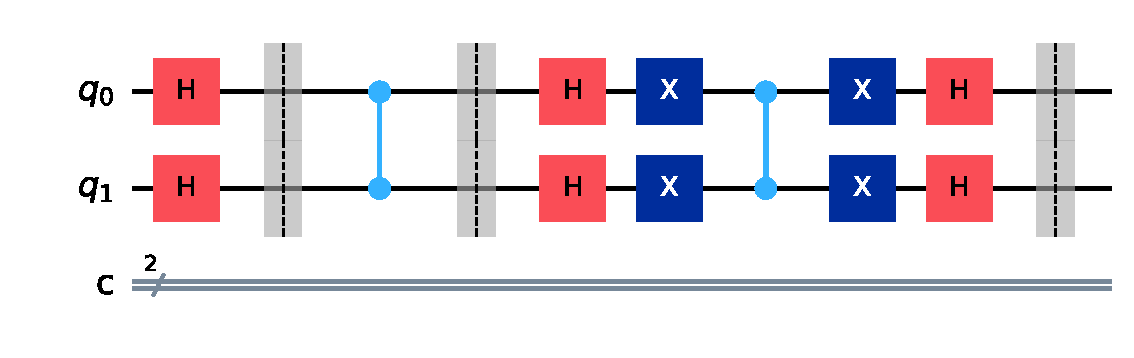
\includegraphics[keepaspectratio]{apostila_files/figure-pdf/cell-126-output-1.pdf}}

\pandocbounded{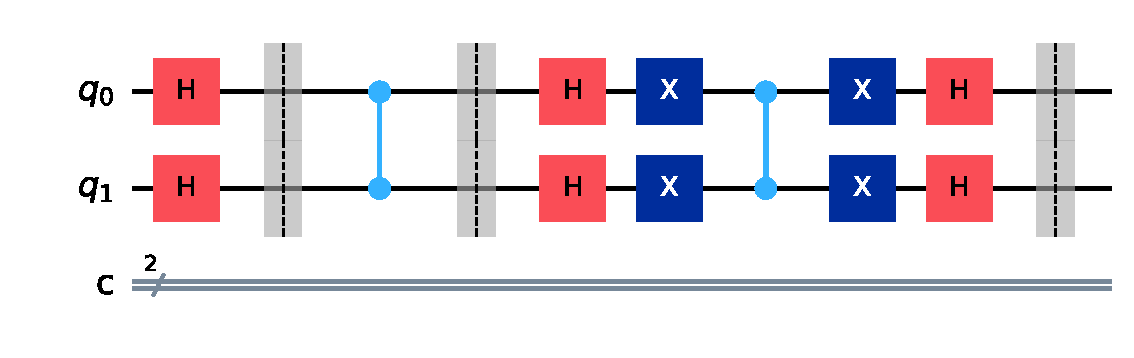
\includegraphics[keepaspectratio]{apostila_files/figure-pdf/cell-126-output-2.pdf}}

\subsubsection{Passo 4: Medição}\label{passo-4-mediuxe7uxe3o}

Finalmente, medimos o estado do sistema quântico. Após a aplicação do
oráculo e do difusor, o estado do sistema é \(|11\rangle\) com
probabilidade 100\%. Portanto, ao medir os qubits, obtemos o resultado
\texttt{11} com certeza.

\begin{Shaded}
\begin{Highlighting}[]
\CommentTok{\# Finalização com medição nos qubits}
\NormalTok{qc.measure([}\DecValTok{0}\NormalTok{, }\DecValTok{1}\NormalTok{], [}\DecValTok{0}\NormalTok{, }\DecValTok{1}\NormalTok{])}
\NormalTok{qc.draw(}\StringTok{\textquotesingle{}mpl\textquotesingle{}}\NormalTok{)}
\end{Highlighting}
\end{Shaded}

\pandocbounded{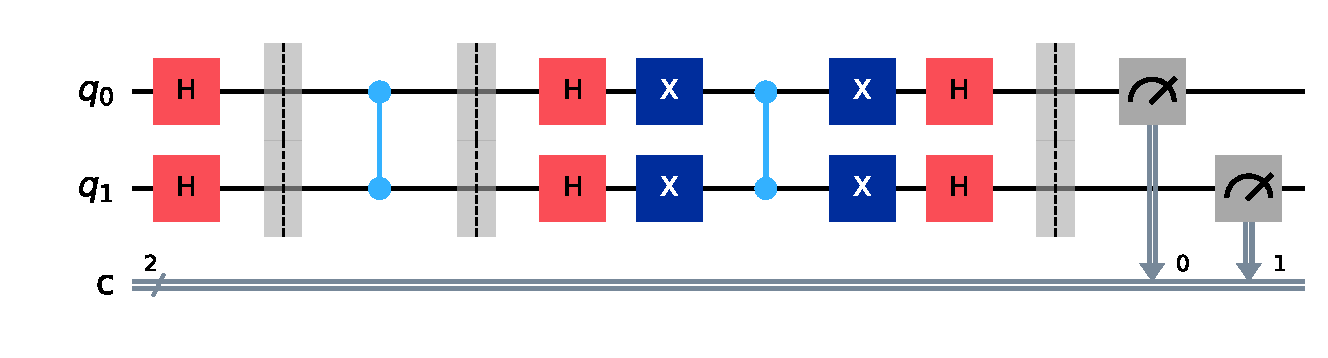
\includegraphics[keepaspectratio]{apostila_files/figure-pdf/cell-127-output-1.pdf}}

\pandocbounded{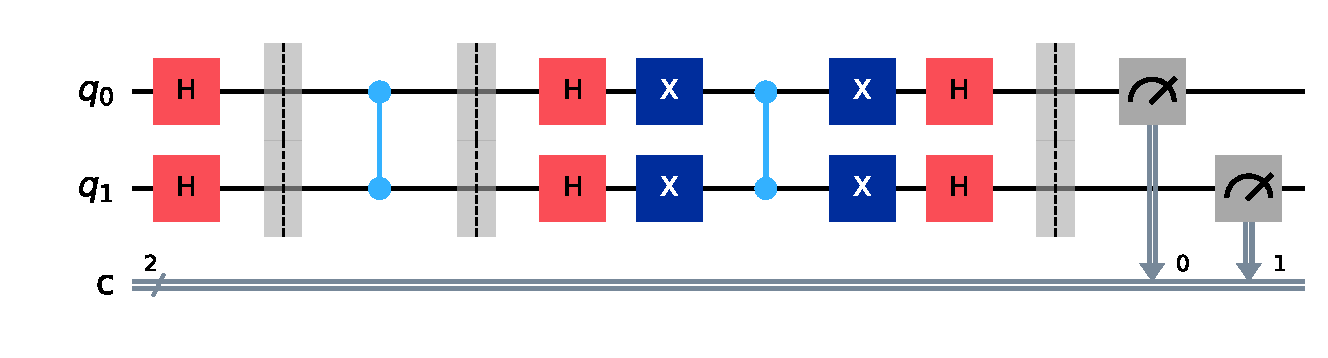
\includegraphics[keepaspectratio]{apostila_files/figure-pdf/cell-127-output-2.pdf}}

\subsubsection{Passo 5: Execução do
Circuito}\label{passo-5-execuuxe7uxe3o-do-circuito}

Aqui o circuito é executado no simulador quântico, coletando os
resultados das medições para verificar se o algoritmo funcionou conforme
esperado.

\begin{Shaded}
\begin{Highlighting}[]
\CommentTok{\# {-}{-}{-} EXECUÇÃO {-}{-}{-}}
\NormalTok{simulador }\OperatorTok{=}\NormalTok{ AerSimulator()}
\NormalTok{job }\OperatorTok{=}\NormalTok{ simulador.run(transpile(qc, simulador), shots}\OperatorTok{=}\DecValTok{1024}\NormalTok{)   }
\NormalTok{resultado }\OperatorTok{=}\NormalTok{ job.result().get\_counts()}

\BuiltInTok{print}\NormalTok{(}\StringTok{"}\CharTok{\textbackslash{}n}\StringTok{{-}{-}{-} Resultado da Busca {-}{-}{-}"}\NormalTok{)}
\BuiltInTok{print}\NormalTok{(}\SpecialStringTok{f"Contagens: }\SpecialCharTok{\{}\NormalTok{resultado}\SpecialCharTok{\}}\SpecialStringTok{"}\NormalTok{)}
\CommentTok{\# Deve ser 100\% (ou muito próximo) em \textquotesingle{}11\textquotesingle{}}
\end{Highlighting}
\end{Shaded}

\begin{verbatim}

--- Resultado da Busca ---
Contagens: {'11': 1024}
\end{verbatim}

\begin{verbatim}

--- Resultado da Busca ---
Contagens: {'11': 1024}
\end{verbatim}

\newpage

\chapter{Módulo 11: QFT e Estimação de
Fase}\label{muxf3dulo-11-qft-e-estimauxe7uxe3o-de-fase}

\chapter{Aula 11 --- Transformada de Fourier Quântica e Estimação de
Fase}\label{aula-11-transformada-de-fourier-quuxe2ntica-e-estimauxe7uxe3o-de-fase}

\chapter{Visualizando a Transformada de Fourier Quântica (QFT) com
Esferas de
Bloch}\label{visualizando-a-transformada-de-fourier-quuxe2ntica-qft-com-esferas-de-bloch}

A \textbf{Transformada de Fourier Quântica (QFT)} é, essencialmente, uma
máquina de \textbf{tradução}.

\begin{itemize}
\tightlist
\item
  \textbf{Língua 1 (Base Computacional):} Você guarda informação ligando
  ou desligando switches (0 ou 1). É digital.
\item
  \textbf{Língua 2 (Base de Fourier):} Você guarda informação na
  \textbf{fase} (na rotação) dos qubits. É analógico/ondulatório.
\end{itemize}

\subsection{A Analogia do Relógio}\label{a-analogia-do-reluxf3gio}

Imagine que você quer representar o número \textbf{6}.

\begin{enumerate}
\def\labelenumi{\arabic{enumi}.}
\tightlist
\item
  \textbf{Jeito Clássico (Binário):} Você escreve \texttt{110}.
\end{enumerate}

\begin{itemize}
\tightlist
\item
  Qubit 2: Ligado (1)
\item
  Qubit 1: Ligado (1)
\item
  Qubit 0: Desligado (0)
\item
  \emph{Visual na Esfera:} Setas apontando para Baixo, Baixo, Cima.
\end{itemize}

\begin{enumerate}
\def\labelenumi{\arabic{enumi}.}
\setcounter{enumi}{1}
\tightlist
\item
  \textbf{Jeito QFT (Rotação):} A QFT pega esses bits e transforma todos
  os qubits para a linha do Equador (Superposição). A informação ``6''
  não está mais no ``Cima/Baixo'', mas no \textbf{ângulo} para onde a
  seta aponta no horizonte.
\end{enumerate}

\begin{itemize}
\tightlist
\item
  Um qubit gira um pouco.
\item
  O outro gira o dobro.
\item
  O outro gira o quádruplo.
\end{itemize}

A QFT codifica o \textbf{valor} do número na \textbf{frequência de
rotação} das fases.

\subsection{O Experimento Visual}\label{o-experimento-visual}

Vamos usar o Qiskit para ver isso acontecer. Vamos pegar o número 6
(\texttt{110}), aplicar a QFT e ver como as Esferas de Bloch mudam.

Para facilitar, usaremos a biblioteca pronta de QFT do Qiskit
(\texttt{qiskit.circuit.library}), assim focamos no efeito e não na
montagem manual das portas agora.

\begin{Shaded}
\begin{Highlighting}[]
\ImportTok{import}\NormalTok{ numpy }\ImportTok{as}\NormalTok{ np}
\ImportTok{from}\NormalTok{ qiskit }\ImportTok{import}\NormalTok{ QuantumCircuit, transpile}
\ImportTok{from}\NormalTok{ qiskit.circuit.library }\ImportTok{import}\NormalTok{ QFT}
\ImportTok{from}\NormalTok{ qiskit.quantum\_info }\ImportTok{import}\NormalTok{ Statevector}
\ImportTok{from}\NormalTok{ qiskit.visualization }\ImportTok{import}\NormalTok{ plot\_bloch\_multivector}
\ImportTok{import}\NormalTok{ matplotlib.pyplot }\ImportTok{as}\NormalTok{ plt}
\end{Highlighting}
\end{Shaded}

\begin{Shaded}
\begin{Highlighting}[]
\CommentTok{\# 1. PREPARAÇÃO: Codificar o número 6 (Binário 110)}
\CommentTok{\# Em Qiskit (Little Endian): q0 é o menos significativo.}
\CommentTok{\# 6 = 0 * (2\^{}0) + 1 * (2\^{}1) + 1 * (2\^{}2) {-}\textgreater{} q0=0, q1=1, q2=1}
\NormalTok{num\_qubits }\OperatorTok{=} \DecValTok{3}
\NormalTok{qc }\OperatorTok{=}\NormalTok{ QuantumCircuit(num\_qubits)}

\CommentTok{\# Codificando o \textquotesingle{}6\textquotesingle{} (Portas X onde o bit é 1)}
\CommentTok{\# qc.x(0) \# q0 = 0 (não fazemos nada)}
\NormalTok{qc.x(}\DecValTok{1}\NormalTok{) }\CommentTok{\# q1 = 1}
\NormalTok{qc.x(}\DecValTok{2}\NormalTok{) }\CommentTok{\# q2 = 1}

\CommentTok{\# Vamos salvar o estado visual ANTES da QFT}
\NormalTok{estado\_antes }\OperatorTok{=}\NormalTok{ Statevector(qc)}
\BuiltInTok{print}\NormalTok{(}\StringTok{"{-}{-}{-} Estado Antes (Binário 110) {-}{-}{-}"}\NormalTok{)}
\CommentTok{\# Vai mostrar setas para baixo (1) e para cima (0)}
\end{Highlighting}
\end{Shaded}

\begin{verbatim}
--- Estado Antes (Binário 110) ---
\end{verbatim}

\begin{verbatim}
--- Estado Antes (Binário 110) ---
\end{verbatim}

\begin{Shaded}
\begin{Highlighting}[]
\CommentTok{\# 2. A MÁGICA: Aplicar a QFT}
\CommentTok{\# A biblioteca cria o circuito complexo de Hadamards e Rotações para nós}
\NormalTok{qc\_qft }\OperatorTok{=}\NormalTok{ QFT(num\_qubits, do\_swaps}\OperatorTok{=}\VariableTok{False}\NormalTok{).to\_gate()}
\NormalTok{qc.append(qc\_qft, }\BuiltInTok{range}\NormalTok{(num\_qubits))}

\CommentTok{\# Vamos salvar o estado visual DEPOIS da QFT}
\NormalTok{estado\_depois }\OperatorTok{=}\NormalTok{ Statevector(qc)}

\CommentTok{\# Desenha o circuito completo}
\NormalTok{qc.draw(}\StringTok{\textquotesingle{}mpl\textquotesingle{}}\NormalTok{) }
\end{Highlighting}
\end{Shaded}

\begin{verbatim}
/tmp/ipykernel_666762/638381934.py:3: DeprecationWarning: The class ``qiskit.circuit.library.basis_change.qft.QFT`` is deprecated as of Qiskit 2.1. It will be removed in Qiskit 3.0. ('Use qiskit.circuit.library.QFTGate or qiskit.synthesis.qft.synth_qft_full instead, for access to all previous arguments.',)
  qc_qft = QFT(num_qubits, do_swaps=False).to_gate()
\end{verbatim}

\pandocbounded{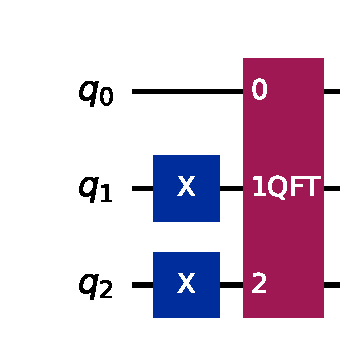
\includegraphics[keepaspectratio]{apostila_files/figure-pdf/cell-131-output-2.pdf}}

\pandocbounded{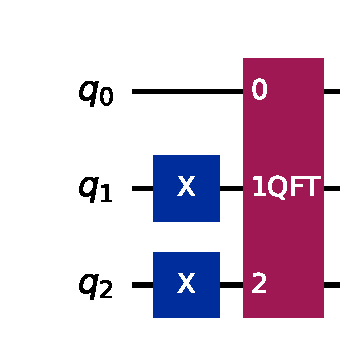
\includegraphics[keepaspectratio]{apostila_files/figure-pdf/cell-131-output-3.pdf}}

\begin{verbatim}
C:\Users\Max\AppData\Local\Temp\ipykernel_18328\3244769350.py:3: DeprecationWarning: The class ``qiskit.circuit.library.basis_change.qft.QFT`` is deprecated as of Qiskit 2.1. It will be removed in Qiskit 3.0. ('Use qiskit.circuit.library.QFTGate or qiskit.synthesis.qft.synth_qft_full instead, for access to all previous arguments.',)
  qc_qft = QFT(num_qubits, do_swaps=False).to_gate()
\end{verbatim}

\begin{Shaded}
\begin{Highlighting}[]
\ImportTok{from}\NormalTok{ IPython.display }\ImportTok{import}\NormalTok{ display}

\CommentTok{\# 3. VISUALIZAÇÃO}
\BuiltInTok{print}\NormalTok{(}\StringTok{"}\CharTok{\textbackslash{}n}\StringTok{{-}{-}{-} Gerando Esferas de Bloch... {-}{-}{-}"}\NormalTok{)}

\CommentTok{\# Plot 1: Binário Puro}
\NormalTok{fig1 }\OperatorTok{=}\NormalTok{ plot\_bloch\_multivector(estado\_antes, title}\OperatorTok{=}\StringTok{"Antes: Número 6 (Base Computacional)"}\NormalTok{)}
\NormalTok{display(fig1)}

\CommentTok{\# Plot 2: Fourier}
\NormalTok{fig2 }\OperatorTok{=}\NormalTok{ plot\_bloch\_multivector(estado\_depois, title}\OperatorTok{=}\StringTok{"Depois: Número 6 (Base de Fourier)"}\NormalTok{)}
\NormalTok{display(fig2)}
\end{Highlighting}
\end{Shaded}

\begin{verbatim}

--- Gerando Esferas de Bloch... ---
\end{verbatim}

\pandocbounded{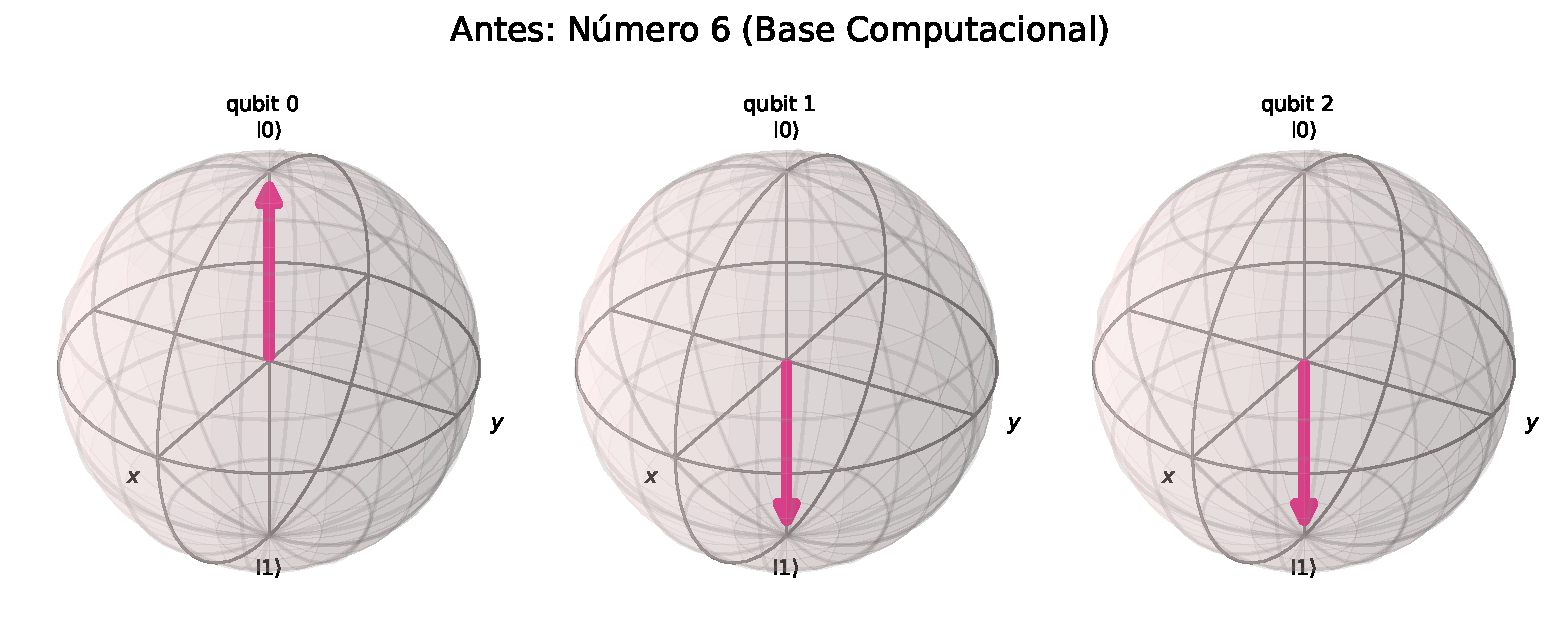
\includegraphics[keepaspectratio]{apostila_files/figure-pdf/cell-132-output-2.pdf}}

\pandocbounded{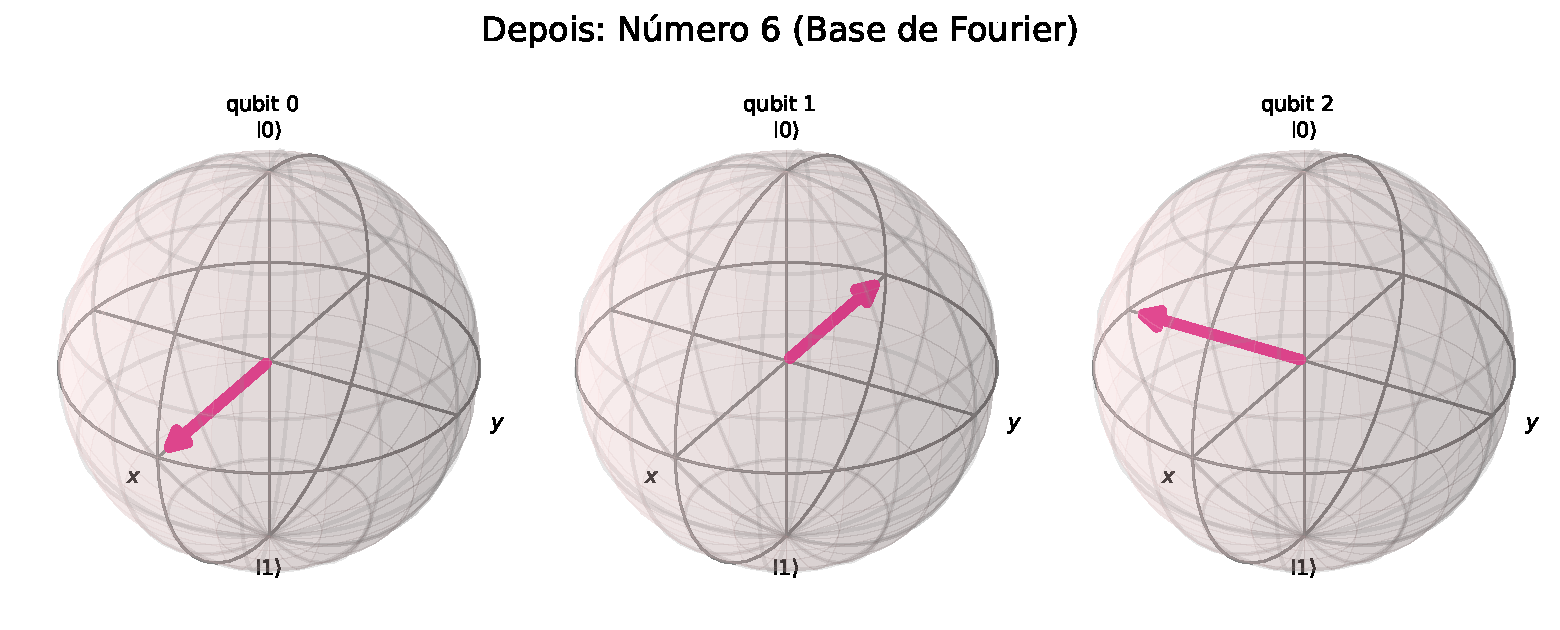
\includegraphics[keepaspectratio]{apostila_files/figure-pdf/cell-132-output-3.pdf}}

\pandocbounded{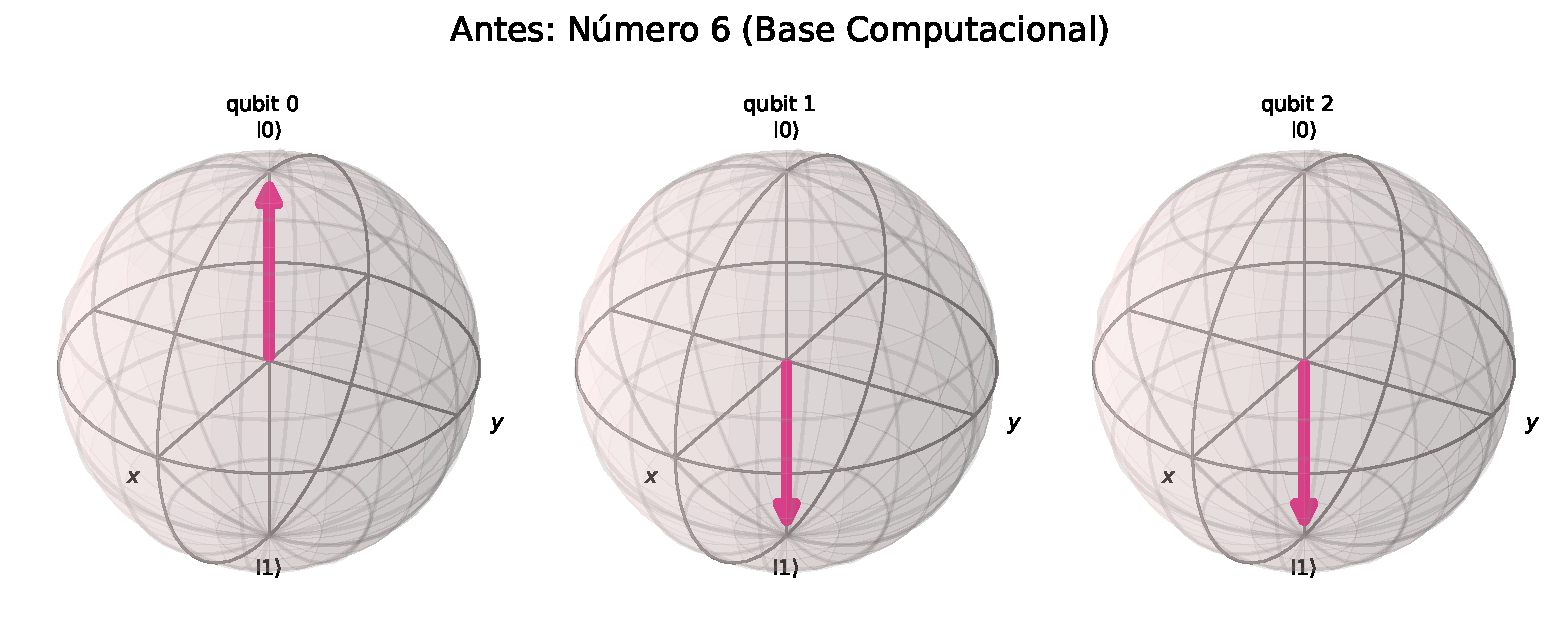
\includegraphics[keepaspectratio]{apostila_files/figure-pdf/cell-132-output-4.pdf}}

\pandocbounded{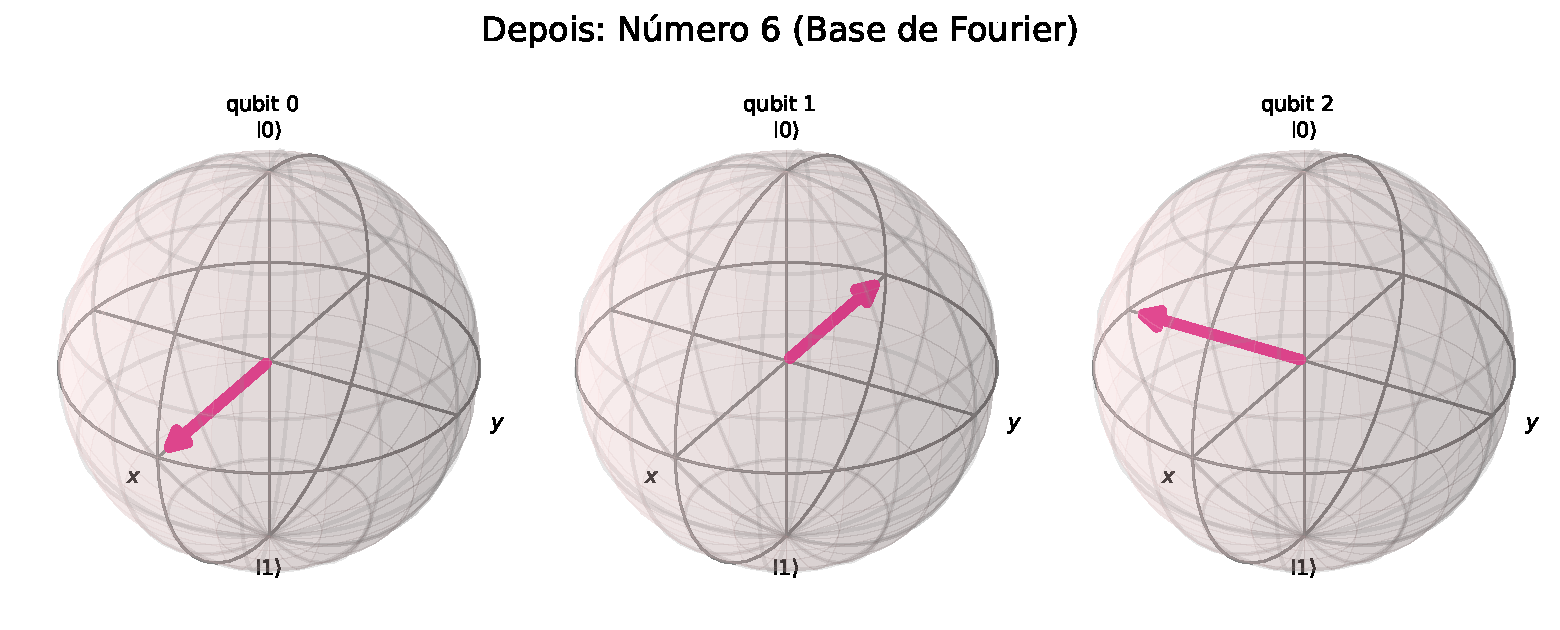
\includegraphics[keepaspectratio]{apostila_files/figure-pdf/cell-132-output-5.pdf}}

\begin{verbatim}

--- Gerando Esferas de Bloch... ---
\end{verbatim}

\subsection{O que você vai ver nas
imagens:}\label{o-que-vocuxea-vai-ver-nas-imagens}

\begin{enumerate}
\def\labelenumi{\arabic{enumi}.}
\tightlist
\item
  \textbf{Imagem ``Antes'':}
\end{enumerate}

\begin{itemize}
\tightlist
\item
  Qubits apontam para o Pólo Sul (1) ou Norte (0). Nada de novo.
\end{itemize}

\begin{enumerate}
\def\labelenumi{\arabic{enumi}.}
\setcounter{enumi}{1}
\tightlist
\item
  \textbf{Imagem ``Depois'' (A parte interessante):}
\end{enumerate}

\begin{itemize}
\tightlist
\item
  \textbf{Todos} os qubits estão na linha do Equador (a seta vermelha
  está deitada). Isso significa que todos têm 50\% de chance de ser 0 ou
  1.
\item
  \textbf{A Diferença:} Olhe para a direção da seta no plano XY (a
  rotação).
\item
  O \textbf{Qubit 2} girou um ângulo específico.
\item
  O \textbf{Qubit 1} girou o dobro desse ângulo.
\item
  O \textbf{Qubit 0} girou ainda mais.
\end{itemize}

Se você mudasse o código para codificar o número \textbf{1}, as setas
girariam muito pouco. Se codificasse o \textbf{7}, elas girariam quase a
volta toda.

\subsection{Por que isso é útil? (A Intuição do Algoritmo de
Shor)}\label{por-que-isso-uxe9-uxfatil-a-intuiuxe7uxe3o-do-algoritmo-de-shor}

Aqui está o ``pulo do gato'' para a fatoração:

Computadores clássicos são ruins em achar \textbf{periodicidade}
(padrões que se repetem) em dados gigantes. Computadores quânticos,
usando a QFT, transformam esse problema de ``achar padrão'' em um
problema de ``medir rotação''.

\begin{enumerate}
\def\labelenumi{\arabic{enumi}.}
\tightlist
\item
  Você cria uma superposição de todos os números possíveis.
\item
  Você faz um cálculo matemático modular (o coração do algoritmo de
  Shor).
\item
  As respostas ``erradas'' criam interferência destrutiva.
\item
  As respostas ``certas'' criam um padrão de rotação construtivo.
\item
  Você aplica a \textbf{QFT Inversa}. Ela traduz essas rotações de volta
  para números binários (0 e 1).
\item
  O resultado que você mede é o \textbf{período} da função, que é a
  chave para quebrar a senha RSA.
\end{enumerate}

\subsection{Desafio Prático}\label{desafio-pruxe1tico}

Tente alterar o código acima. Onde tem \texttt{qc.x(1)} e
\texttt{qc.x(2)} (número 6), deixe apenas \texttt{qc.x(0)} (número 1) e
rode novamente. Observe como as setas na imagem ``Depois'' giram muito
menos. Essa sensibilidade visual é a essência da ``frequência''.

\subsection{Interpretação dos resultados baseados na precisão dos
qubits}\label{interpretauxe7uxe3o-dos-resultados-baseados-na-precisuxe3o-dos-qubits}

\begin{Shaded}
\begin{Highlighting}[]
\CommentTok{\# Visualizar o vetor de estados com melhor formatação}
\BuiltInTok{print}\NormalTok{(}\StringTok{"}\CharTok{\textbackslash{}n}\StringTok{=== ESTADO ANTES DA QFT (Base Computacional) ==="}\NormalTok{)}
\BuiltInTok{print}\NormalTok{(}\SpecialStringTok{f"Representação: |110⟩ (número 6 em binário)"}\NormalTok{)}
\NormalTok{display(estado\_antes.draw(}\StringTok{\textquotesingle{}latex\textquotesingle{}}\NormalTok{))}
\BuiltInTok{print}\NormalTok{(}\SpecialStringTok{f"}\CharTok{\textbackslash{}n}\SpecialStringTok{Amplitudes:"}\NormalTok{)}
\ControlFlowTok{for}\NormalTok{ i, amp }\KeywordTok{in} \BuiltInTok{enumerate}\NormalTok{(estado\_antes.data):}
    \ControlFlowTok{if} \BuiltInTok{abs}\NormalTok{(amp) }\OperatorTok{\textgreater{}} \FloatTok{1e{-}10}\NormalTok{:  }\CommentTok{\# Mostrar apenas amplitudes não{-}zero}
        \BuiltInTok{print}\NormalTok{(}\SpecialStringTok{f"  |}\SpecialCharTok{\{}\NormalTok{i}\SpecialCharTok{:03b\}}\SpecialStringTok{⟩: }\SpecialCharTok{\{}\NormalTok{amp}\SpecialCharTok{.}\NormalTok{real}\SpecialCharTok{:+.8f\}}\SpecialStringTok{ }\SpecialCharTok{\{}\NormalTok{amp}\SpecialCharTok{.}\NormalTok{imag}\SpecialCharTok{:+.8f\}}\SpecialStringTok{j  (|amp| = }\SpecialCharTok{\{}\BuiltInTok{abs}\NormalTok{(amp)}\SpecialCharTok{:.8f\}}\SpecialStringTok{)"}\NormalTok{)}
\end{Highlighting}
\end{Shaded}

\begin{verbatim}

=== ESTADO ANTES DA QFT (Base Computacional) ===
Representação: |110⟩ (número 6 em binário)
\end{verbatim}

$$ |110\rangle$$

\begin{verbatim}

Amplitudes:
  |110⟩: +1.00000000 +0.00000000j  (|amp| = 1.00000000)
\end{verbatim}

\begin{verbatim}

=== ESTADO ANTES DA QFT (Base Computacional) ===
Representação: |110⟩ (número 6 em binário)
\end{verbatim}

\begin{verbatim}

Amplitudes:
  |110⟩: +1.00000000 +0.00000000j  (|amp| = 1.00000000)
\end{verbatim}

\begin{Shaded}
\begin{Highlighting}[]
\BuiltInTok{print}\NormalTok{(}\StringTok{"}\CharTok{\textbackslash{}n}\StringTok{"} \OperatorTok{+} \StringTok{"="}\OperatorTok{*}\DecValTok{60}\NormalTok{)}
\BuiltInTok{print}\NormalTok{(}\StringTok{"}\CharTok{\textbackslash{}n}\StringTok{=== ESTADO DEPOIS DA QFT (Base de Fourier) ==="}\NormalTok{)}
\BuiltInTok{print}\NormalTok{(}\SpecialStringTok{f"Informação codificada nas fases (rotações)"}\NormalTok{)}
\NormalTok{display(estado\_depois.draw(}\StringTok{\textquotesingle{}latex\textquotesingle{}}\NormalTok{))}
\BuiltInTok{print}\NormalTok{(}\SpecialStringTok{f"}\CharTok{\textbackslash{}n}\SpecialStringTok{Amplitudes α, β, ... (note os valores complexos):"}\NormalTok{)}
\ControlFlowTok{for}\NormalTok{ i, amp }\KeywordTok{in} \BuiltInTok{enumerate}\NormalTok{(estado\_depois.data):}
    \BuiltInTok{print}\NormalTok{(}\SpecialStringTok{f"Estado |}\SpecialCharTok{\{}\NormalTok{i}\SpecialCharTok{:03b\}}\SpecialStringTok{⟩: }\SpecialCharTok{\{}\NormalTok{amp}\SpecialCharTok{.}\NormalTok{real}\SpecialCharTok{:+.8f\}}\SpecialStringTok{ }\SpecialCharTok{\{}\NormalTok{amp}\SpecialCharTok{.}\NormalTok{imag}\SpecialCharTok{:+.8f\}}\SpecialStringTok{j"}\NormalTok{)}

\CommentTok{\# Mostrar as fases de cada amplitude}
\BuiltInTok{print}\NormalTok{(}\StringTok{"}\CharTok{\textbackslash{}n}\StringTok{{-}{-}{-} Fases (ângulos) de cada amplitude {-}{-}{-}"}\NormalTok{)}
\NormalTok{fases }\OperatorTok{=}\NormalTok{ np.angle(estado\_depois.data, deg}\OperatorTok{=}\VariableTok{True}\NormalTok{)}
\ControlFlowTok{for}\NormalTok{ i, fase }\KeywordTok{in} \BuiltInTok{enumerate}\NormalTok{(fases):}
    \BuiltInTok{print}\NormalTok{(}\SpecialStringTok{f"Estado |}\SpecialCharTok{\{}\NormalTok{i}\SpecialCharTok{:03b\}}\SpecialStringTok{⟩: Fase = }\SpecialCharTok{\{}\NormalTok{fase}\SpecialCharTok{:7.2f\}}\SpecialStringTok{°"}\NormalTok{)}
\end{Highlighting}
\end{Shaded}

\begin{verbatim}

============================================================

=== ESTADO DEPOIS DA QFT (Base de Fourier) ===
Informação codificada nas fases (rotações)
\end{verbatim}

$$\frac{\sqrt{2}}{4} |000\rangle+\frac{\sqrt{2}}{4} |001\rangle- \frac{\sqrt{2}}{4} |010\rangle- \frac{\sqrt{2}}{4} |011\rangle- \frac{\sqrt{2} i}{4} |100\rangle- \frac{\sqrt{2} i}{4} |101\rangle+\frac{\sqrt{2} i}{4} |110\rangle+\frac{\sqrt{2} i}{4} |111\rangle$$

\begin{verbatim}

Amplitudes α, β, ... (note os valores complexos):
Estado |000⟩: +0.35355339 +0.00000000j
Estado |001⟩: +0.35355339 +0.00000000j
Estado |010⟩: -0.35355339 +0.00000000j
Estado |011⟩: -0.35355339 +0.00000000j
Estado |100⟩: -0.00000000 -0.35355339j
Estado |101⟩: -0.00000000 -0.35355339j
Estado |110⟩: +0.00000000 +0.35355339j
Estado |111⟩: +0.00000000 +0.35355339j

--- Fases (ângulos) de cada amplitude ---
Estado |000⟩: Fase =    0.00°
Estado |001⟩: Fase =    0.00°
Estado |010⟩: Fase =  180.00°
Estado |011⟩: Fase =  180.00°
Estado |100⟩: Fase =  -90.00°
Estado |101⟩: Fase =  -90.00°
Estado |110⟩: Fase =   90.00°
Estado |111⟩: Fase =   90.00°
\end{verbatim}

\begin{verbatim}

============================================================

=== ESTADO DEPOIS DA QFT (Base de Fourier) ===
Informação codificada nas fases (rotações)
\end{verbatim}

\begin{verbatim}

Amplitudes α, β, ... (note os valores complexos):
Estado |000⟩: +0.35355339 +0.00000000j
Estado |001⟩: +0.35355339 +0.00000000j
Estado |010⟩: -0.35355339 +0.00000000j
Estado |011⟩: -0.35355339 +0.00000000j
Estado |100⟩: -0.00000000 -0.35355339j
Estado |101⟩: -0.00000000 -0.35355339j
Estado |110⟩: +0.00000000 +0.35355339j
Estado |111⟩: +0.00000000 +0.35355339j

--- Fases (ângulos) de cada amplitude ---
Estado |000⟩: Fase =    0.00°
Estado |001⟩: Fase =    0.00°
Estado |010⟩: Fase =  180.00°
Estado |011⟩: Fase =  180.00°
Estado |100⟩: Fase =  -90.00°
Estado |101⟩: Fase =  -90.00°
Estado |110⟩: Fase =   90.00°
Estado |111⟩: Fase =   90.00°
\end{verbatim}

\section{QFT Inversa e Estimação de Fase Quântica
(QPE)}\label{qft-inversa-e-estimauxe7uxe3o-de-fase-quuxe2ntica-qpe}

A capacidade de ``ver'' os qubits girando é o superpoder de quem
trabalha com algoritmos quânticos.

Agora, vamos fechar este ciclo com a \textbf{``Killer App''} da QFT.

Você aprendeu que a QFT traduz \textbf{Bits --\textgreater{} Rotação}.
Logicamente, deve existir uma \textbf{QFT Inversa (\(QFT^\dagger\))} que
traduz \textbf{Rotação --\textgreater{} Bits}.

É aqui que entra a \textbf{Estimação de Fase Quântica (QPE - Quantum
Phase Estimation)}.

\subsection{O Conceito: O ``Velocímetro''
Quântico}\label{o-conceito-o-velocuxedmetro-quuxe2ntico}

Imagine que você tem uma porta lógica misteriosa (vamos chamá-la de
\(U\)). Quando você passa um qubit por ela, ela não muda o valor (0
continua 0, 1 continua 1), mas ela ``chuta'' a fase, girando o qubit num
ângulo \(\theta\) desconhecido.

\textbf{O Problema:} Como você descobre esse ângulo \(\theta\) com
precisão? Lembre-se: medir um qubit destrói a fase. Você não pode
simplesmente pegar um transferidor e medir o ângulo na Esfera de Bloch.

\textbf{A Solução (QPE):} O algoritmo QPE funciona como um
\textbf{estroboscópio} (aquela luz piscante de festas) para medir a
velocidade de um ventilador.

\begin{enumerate}
\def\labelenumi{\arabic{enumi}.}
\tightlist
\item
  Você aplica a porta \(U\) várias vezes (rotações acumuladas).
\item
  Você usa o ``Phase Kickback'' (que você já aprendeu!) para copiar essa
  rotação para qubits auxiliares.
\item
  Esses auxiliares ficam com a informação da rotação codificada nas suas
  fases.
\item
  Você aplica a \textbf{QFT Inversa} para traduzir essas fases em
  números binários (0 e 1).
\item
  O resultado da medição é o ângulo exato!
\end{enumerate}

\subsection{O Experimento em Python}\label{o-experimento-em-python}

Vamos criar uma porta que gira o qubit em exatamente \(1/8\) \textbf{de
volta} (fase de \(45^\circ\) ou \(\frac{\pi}{4}\)). Vamos fingir que não
sabemos esse valor e pedir para o algoritmo QPE descobrir.

O resultado esperado em binário fracionário:

Em binário: (O terceiro bit é 1).

\begin{Shaded}
\begin{Highlighting}[]
\ImportTok{import}\NormalTok{ numpy }\ImportTok{as}\NormalTok{ np}
\ImportTok{from}\NormalTok{ qiskit }\ImportTok{import}\NormalTok{ QuantumCircuit, transpile}
\ImportTok{from}\NormalTok{ qiskit\_aer }\ImportTok{import}\NormalTok{ AerSimulator}
\ImportTok{from}\NormalTok{ qiskit.circuit.library }\ImportTok{import}\NormalTok{ QFT, PhaseGate}
\ImportTok{from}\NormalTok{ qiskit.visualization }\ImportTok{import}\NormalTok{ plot\_histogram}
\end{Highlighting}
\end{Shaded}

\begin{Shaded}
\begin{Highlighting}[]
\CommentTok{\# {-}{-}{-} 1. CONFIGURAÇÃO {-}{-}{-}}
\CommentTok{\# Precisamos de qubits para "contar" a fase (precisão) e 1 (q3) para sofrer a ação}
\NormalTok{num\_qubits\_contagem }\OperatorTok{=} \DecValTok{3} 
\NormalTok{num\_qubits\_total }\OperatorTok{=}\NormalTok{ num\_qubits\_contagem }\OperatorTok{+} \DecValTok{1} \CommentTok{\# +1 para o alvo}

\NormalTok{qc }\OperatorTok{=}\NormalTok{ QuantumCircuit(num\_qubits\_total, num\_qubits\_contagem)}
\NormalTok{qc.draw(}\StringTok{\textquotesingle{}mpl\textquotesingle{}}\NormalTok{)}
\end{Highlighting}
\end{Shaded}

\pandocbounded{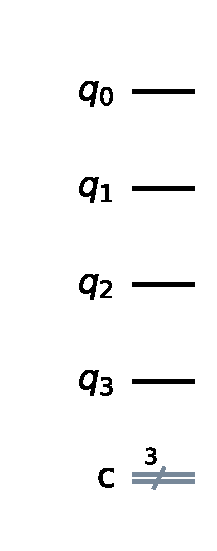
\includegraphics[keepaspectratio]{apostila_files/figure-pdf/cell-136-output-1.pdf}}

\pandocbounded{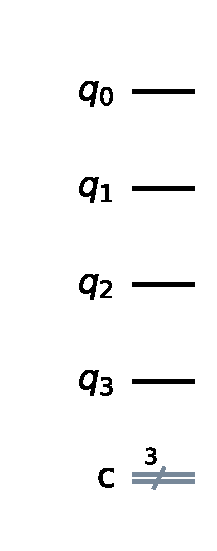
\includegraphics[keepaspectratio]{apostila_files/figure-pdf/cell-136-output-2.pdf}}

\begin{Shaded}
\begin{Highlighting}[]
\CommentTok{\# {-}{-}{-} 2. PREPARAÇÃO {-}{-}{-}}
\CommentTok{\# Colocar os qubits de contagem em superposição (para receberem o kickback)}
\ControlFlowTok{for}\NormalTok{ qubit }\KeywordTok{in} \BuiltInTok{range}\NormalTok{(num\_qubits\_contagem):}
\NormalTok{    qc.h(qubit)}

\CommentTok{\# Colocar o qubit alvo (o último) no estado |1\textgreater{}}
\CommentTok{\# (O Kickback só funciona se o alvo for |1\textgreater{}, lembre{-}se do eigenstate)}
\NormalTok{qc.x(num\_qubits\_contagem)}
\NormalTok{qc.draw(}\StringTok{\textquotesingle{}mpl\textquotesingle{}}\NormalTok{)}
\end{Highlighting}
\end{Shaded}

\pandocbounded{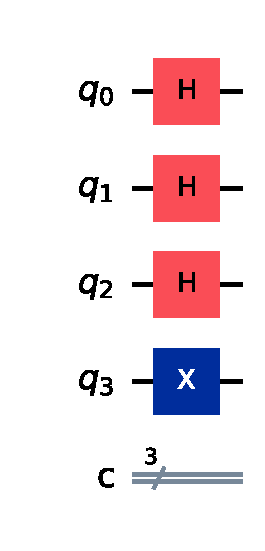
\includegraphics[keepaspectratio]{apostila_files/figure-pdf/cell-137-output-1.pdf}}

\pandocbounded{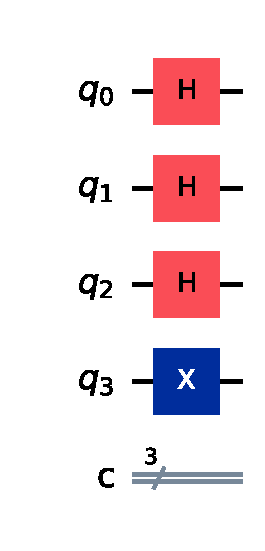
\includegraphics[keepaspectratio]{apostila_files/figure-pdf/cell-137-output-2.pdf}}

\begin{Shaded}
\begin{Highlighting}[]
\CommentTok{\# {-}{-}{-} 3. APLICAÇÃO DA PORTA "MISTERIOSA" (U) {-}{-}{-}}
\CommentTok{\# Vamos definir nossa fase secreta: 1/8 de volta}
\CommentTok{\# Fase = 2 * pi * (1/8)}
\NormalTok{fase\_secreta }\OperatorTok{=} \DecValTok{2} \OperatorTok{*}\NormalTok{ np.pi }\OperatorTok{*}\NormalTok{ (}\DecValTok{1}\OperatorTok{/}\DecValTok{8}\NormalTok{)}

\CommentTok{\# Aplicamos a porta controlada repetidamente (Kickback em cascata)}
\CommentTok{\# Qubit 0 aplica U\^{}1}
\CommentTok{\# Qubit 1 aplica U\^{}2}
\CommentTok{\# Qubit 2 aplica U\^{}4}
\NormalTok{repeticoes }\OperatorTok{=} \DecValTok{1}
\ControlFlowTok{for}\NormalTok{ counting\_qubit }\KeywordTok{in} \BuiltInTok{range}\NormalTok{(num\_qubits\_contagem):}
    \CommentTok{\# PhaseGate Controlada (CP)}
    \CommentTok{\# qc.cp(angulo, controle, alvo). Esta porta foi vista anteriormente.}
\NormalTok{    qc.cp(fase\_secreta }\OperatorTok{*}\NormalTok{ repeticoes, counting\_qubit, num\_qubits\_contagem)}
\NormalTok{    repeticoes }\OperatorTok{=}\NormalTok{ repeticoes }\OperatorTok{*} \DecValTok{2}

\NormalTok{qc.barrier()}
\NormalTok{qc.draw(}\StringTok{\textquotesingle{}mpl\textquotesingle{}}\NormalTok{)}
\end{Highlighting}
\end{Shaded}

\pandocbounded{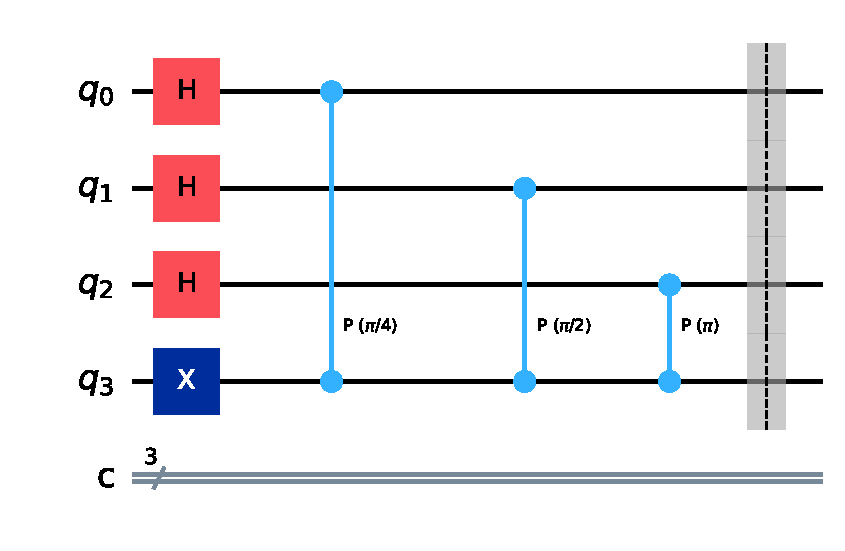
\includegraphics[keepaspectratio]{apostila_files/figure-pdf/cell-138-output-1.pdf}}

\pandocbounded{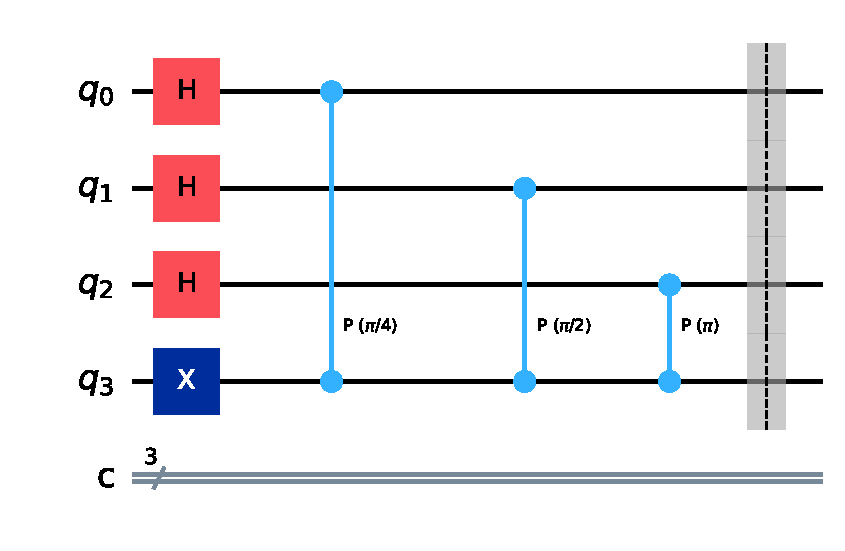
\includegraphics[keepaspectratio]{apostila_files/figure-pdf/cell-138-output-2.pdf}}

\begin{Shaded}
\begin{Highlighting}[]
\CommentTok{\# {-}{-}{-} 4. O DECODIFICADOR (QFT INVERSA) {-}{-}{-}}
\CommentTok{\# Até aqui, a informação do ângulo está escondida na fase dos qubits de contagem.}
\CommentTok{\# A QFT Inversa traduz isso para bits legíveis (0 ou 1).}
\NormalTok{qc\_iqft }\OperatorTok{=}\NormalTok{ QFT(num\_qubits\_contagem, inverse}\OperatorTok{=}\VariableTok{True}\NormalTok{).to\_gate()}
\NormalTok{qc.append(qc\_iqft, }\BuiltInTok{range}\NormalTok{(num\_qubits\_contagem))}
\NormalTok{qc.draw(}\StringTok{\textquotesingle{}mpl\textquotesingle{}}\NormalTok{)}
\end{Highlighting}
\end{Shaded}

\begin{verbatim}
/tmp/ipykernel_666762/3409750826.py:4: DeprecationWarning: The class ``qiskit.circuit.library.basis_change.qft.QFT`` is deprecated as of Qiskit 2.1. It will be removed in Qiskit 3.0. ('Use qiskit.circuit.library.QFTGate or qiskit.synthesis.qft.synth_qft_full instead, for access to all previous arguments.',)
  qc_iqft = QFT(num_qubits_contagem, inverse=True).to_gate()
\end{verbatim}

\pandocbounded{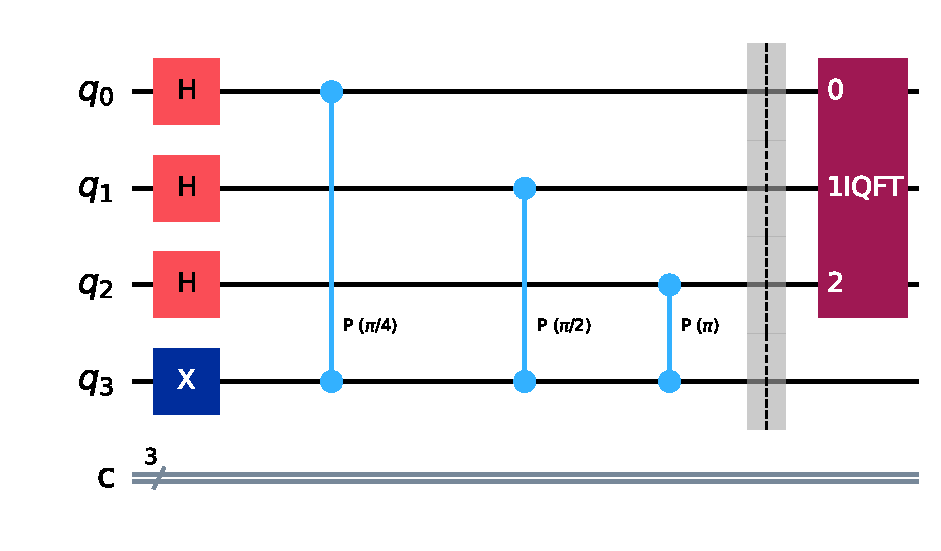
\includegraphics[keepaspectratio]{apostila_files/figure-pdf/cell-139-output-2.pdf}}

\pandocbounded{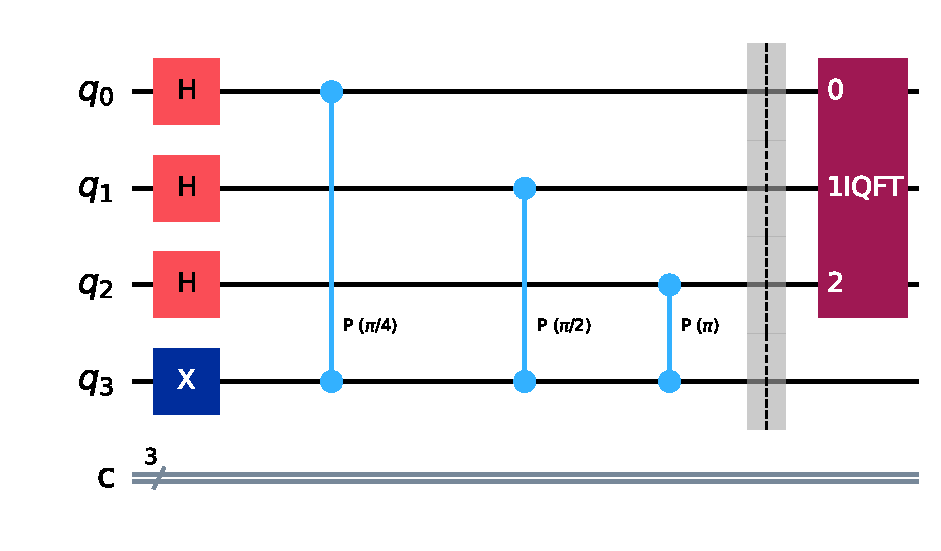
\includegraphics[keepaspectratio]{apostila_files/figure-pdf/cell-139-output-3.pdf}}

\begin{verbatim}
C:\Users\Max\AppData\Local\Temp\ipykernel_18328\2763487660.py:4: DeprecationWarning: The class ``qiskit.circuit.library.basis_change.qft.QFT`` is deprecated as of Qiskit 2.1. It will be removed in Qiskit 3.0. ('Use qiskit.circuit.library.QFTGate or qiskit.synthesis.qft.synth_qft_full instead, for access to all previous arguments.',)
  qc_iqft = QFT(num_qubits_contagem, inverse=True).to_gate()
\end{verbatim}

\begin{Shaded}
\begin{Highlighting}[]
\CommentTok{\# {-}{-}{-} 5. MEDIÇÃO {-}{-}{-}}
\NormalTok{qc.measure(}\BuiltInTok{range}\NormalTok{(num\_qubits\_contagem), }\BuiltInTok{range}\NormalTok{(num\_qubits\_contagem))}
\end{Highlighting}
\end{Shaded}

\begin{verbatim}
<qiskit.circuit.instructionset.InstructionSet at 0x7779dbbcca90>
\end{verbatim}

\begin{Shaded}
\begin{Highlighting}[]
\CommentTok{\# {-}{-}{-} EXECUÇÃO {-}{-}{-}}
\NormalTok{simulador }\OperatorTok{=}\NormalTok{ AerSimulator()}
\NormalTok{job }\OperatorTok{=}\NormalTok{ simulador.run(transpile(qc, simulador), shots}\OperatorTok{=}\DecValTok{1024}\NormalTok{)}
\NormalTok{contagens }\OperatorTok{=}\NormalTok{ job.result().get\_counts()}
\end{Highlighting}
\end{Shaded}

\begin{Shaded}
\begin{Highlighting}[]
\CommentTok{\# {-}{-}{-} INTERPRETAÇÃO {-}{-}{-}}
\CommentTok{\# A saída será um binário, ex: \textquotesingle{}001\textquotesingle{}.}
\CommentTok{\# Isso deve ser lido como fração binária: 0.001}
\CommentTok{\# 0*(1/2) + 0*(1/4) + 1*(1/8) = 1/8.}

\BuiltInTok{print}\NormalTok{(}\StringTok{"}\CharTok{\textbackslash{}n}\StringTok{{-}{-}{-} Resultado da QPE {-}{-}{-}"}\NormalTok{)}
\BuiltInTok{print}\NormalTok{(}\SpecialStringTok{f"Contagens (Binário): }\SpecialCharTok{\{}\NormalTok{contagens}\SpecialCharTok{\}}\SpecialStringTok{"}\NormalTok{)}

\CommentTok{\# Converter o binário mais provável para decimal}
\NormalTok{leitura\_binaria }\OperatorTok{=} \BuiltInTok{list}\NormalTok{(contagens.keys())[}\DecValTok{0}\NormalTok{]}
\NormalTok{decimal }\OperatorTok{=} \BuiltInTok{int}\NormalTok{(leitura\_binaria, }\DecValTok{2}\NormalTok{)}
\NormalTok{fase\_estimada }\OperatorTok{=}\NormalTok{ decimal }\OperatorTok{/}\NormalTok{ (}\DecValTok{2}\OperatorTok{**}\NormalTok{num\_qubits\_contagem)}

\BuiltInTok{print}\NormalTok{(}\SpecialStringTok{f"Binário lido: }\SpecialCharTok{\{}\NormalTok{leitura\_binaria}\SpecialCharTok{\}}\SpecialStringTok{ (Decimal: }\SpecialCharTok{\{}\NormalTok{decimal}\SpecialCharTok{\}}\SpecialStringTok{)"}\NormalTok{)}
\BuiltInTok{print}\NormalTok{(}\SpecialStringTok{f"Fase Estimada: }\SpecialCharTok{\{}\NormalTok{fase\_estimada}\SpecialCharTok{\}}\SpecialStringTok{"}\NormalTok{)}
\BuiltInTok{print}\NormalTok{(}\SpecialStringTok{f"Fase Real Esperada: }\SpecialCharTok{\{}\DecValTok{1}\OperatorTok{/}\DecValTok{8}\SpecialCharTok{\}}\SpecialStringTok{"}\NormalTok{)}
\end{Highlighting}
\end{Shaded}

\begin{verbatim}

--- Resultado da QPE ---
Contagens (Binário): {'001': 1024}
Binário lido: 001 (Decimal: 1)
Fase Estimada: 0.125
Fase Real Esperada: 0.125
\end{verbatim}

\begin{verbatim}

--- Resultado da QPE ---
Contagens (Binário): {'001': 1024}
Binário lido: 001 (Decimal: 1)
Fase Estimada: 0.125
Fase Real Esperada: 0.125
\end{verbatim}

\subsection{Análise do Código}\label{anuxe1lise-do-cuxf3digo}

\begin{enumerate}
\def\labelenumi{\arabic{enumi}.}
\tightlist
\item
  \textbf{O ``Truque'' da Potência:} Você notou o
  \texttt{repeticoes\ *=\ 2}?
\end{enumerate}

\begin{itemize}
\tightlist
\item
  O Qubit 0 verifica a fase uma vez.
\item
  O Qubit 1 verifica a fase duas vezes.
\item
  O Qubit 2 verifica a fase quatro vezes. Isso é exatamente como a
  transformada de Fourier funciona: decompondo o sinal em frequências
  diferentes.
\end{itemize}

\begin{enumerate}
\def\labelenumi{\arabic{enumi}.}
\setcounter{enumi}{1}
\tightlist
\item
  \textbf{A Precisão:} Usamos 3 qubits de contagem. Isso significa que
  podemos medir fases com precisão de até \(1/2^3 = 1/8\). Se a fase
  fosse \(1/16\), precisaríamos de 4 qubits. Se usássemos apenas 3, o
  resultado seria aproximado (probabilístico).
\end{enumerate}

\subsection{Por que isso é a base da quebra de criptografia
(Shor)?}\label{por-que-isso-uxe9-a-base-da-quebra-de-criptografia-shor}

Para quebrar o RSA, precisamos encontrar o período de uma função modular
\(a^x \pmod N\). O Algoritmo de Shor transforma esse problema matemático
num problema de \textbf{estimar a fase} de um operador quântico criado a
partir desse número .

Você acabou de implementar o ``motor'' do algoritmo de Shor. O resto é
apenas aritmética clássica para preparar o problema para o motor rodar.

Você completou o ciclo ``Core'' da computação quântica baseada em gates
(Gate-based Quantum Computing).

\begin{enumerate}
\def\labelenumi{\arabic{enumi}.}
\tightlist
\item
  Álgebra Linear ✅
\item
  Circuitos e Qiskit ✅
\item
  Algoritmos Básicos (Teletransporte, Grover) ✅
\item
  Algoritmos Avançados (QFT, QPE) ✅
\end{enumerate}

\newpage

\chapter{Módulo 12: Hardware Quântico
Real}\label{muxf3dulo-12-hardware-quuxe2ntico-real}

\chapter{Aula 12 --- Hardware Quântico Real: Ruído, Decoerência e
NISQ}\label{aula-12-hardware-quuxe2ntico-real-ruuxeddo-decoeruxeancia-e-nisq}

\section{Executando os circuitos do curso na IBM Quantum
Platform}\label{executando-os-circuitos-do-curso-na-ibm-quantum-platform}

Todos os algoritmos estudados até aqui possuem implementação OpenQASM
pronta para importação no \href{https://quantum.ibm.com/composer}{IBM
Quantum Composer}:

\begin{longtable}[]{@{}
  >{\raggedright\arraybackslash}p{(\linewidth - 2\tabcolsep) * \real{0.5000}}
  >{\raggedright\arraybackslash}p{(\linewidth - 2\tabcolsep) * \real{0.5000}}@{}}
\toprule\noalign{}
\begin{minipage}[b]{\linewidth}\raggedright
Protocolo
\end{minipage} & \begin{minipage}[b]{\linewidth}\raggedright
Arquivo
\end{minipage} \\
\midrule\noalign{}
\endhead
\bottomrule\noalign{}
\endlastfoot
Teletransporte &
\href{./notebooks/qasm/02-teletransport.qasm}{\texttt{notebooks/qasm/02-teletransport.qasm}} \\
Phase Kickback &
\href{./notebooks/qasm/05-kickback.qasm}{\texttt{notebooks/qasm/05-kickback.qasm}} \\
Deutsch-Jozsa &
\href{./notebooks/qasm/05-deutsch-jozsa.qasm}{\texttt{notebooks/qasm/05-deutsch-jozsa.qasm}} \\
Grover &
\href{./notebooks/qasm/06-grover.qasm}{\texttt{notebooks/qasm/06-grover.qasm}} \\
\end{longtable}

\textbf{Roteiro:} importe o arquivo no Composer, execute no simulador
(\texttt{ibmq\_qasm\_simulator}) e depois em um backend real (ex.:
\texttt{ibm\_brisbane}). Compare os histogramas --- em hardware real a
taxa de sucesso fica abaixo de 100\% por causa de \textbf{ruído
quântico}, \textbf{decoerência} e imperfeições dos qubits físicos.

\section{Dispositivos NISQ}\label{dispositivos-nisq}

\chapter{Dispositivos NISQ dependem de integração
quântico-clássica}\label{dispositivos-nisq-dependem-de-integrauxe7uxe3o-quuxe2ntico-cluxe1ssica}

Dispositivos quânticos de escala intermediária e ruidosa não funcionam
como substitutos independentes dos computadores clássicos. A
decoerência, o ruído e a necessidade de repetir medições fazem com que
algoritmos NISQ dependam de controle, otimização e pós-processamento
clássicos.{[}{[}Quantum Computing - Vision and Challenges{]}{]}

A arquitetura mais realista para o estágio atual é híbrida: o computador
clássico coordena o experimento, enquanto o dispositivo quântico executa
subrotinas específicas.

\section{Relações}\label{relauxe7uxf5es}

\begin{itemize}
\tightlist
\item
  {[}\hyperref[vantagem-quuxe2ntica-uxe9-dependente-da-classe-de-problemas]{Vantagem
  quântica é dependente da classe de problemas}{]}
\item
  {[}\hyperref[compilauxe7uxe3o-quuxe2ntica-precisa-respeitar-a-topologia-do-hardware]{Compilação
  quântica precisa respeitar a topologia do hardware}{]}
\end{itemize}

\section{Fonte}\label{fonte}

\begin{itemize}
\tightlist
\item
  {[}1{]} https://arxiv.org/abs/2403.02240
\end{itemize}

\newpage

\chapter{Módulo 13: Quantum Machine Learning
(VQC)}\label{muxf3dulo-13-quantum-machine-learning-vqc}

\chapter{Aula 13 --- Quantum Machine Learning: Classificação com
VQC}\label{aula-13-quantum-machine-learning-classificauxe7uxe3o-com-vqc}

\chapter{Quantum Machine Learning
(QML)}\label{quantum-machine-learning-qml}

🎯 \textbf{Objetivo deste Notebook:} Entender como usar computação
quântica para Machine Learning através de exemplos práticos e visuais.

Bem-vindo ao mundo da \textbf{IA Quântica (Quantum Machine Learning -
QML)}!

Se você já tem experiência com programação e IA clássica, este notebook
vai mostrar como aplicar conceitos familiares (como redes neurais e
classificadores) em computadores quânticos. Vamos usar a biblioteca
\textbf{Qiskit Machine Learning} da IBM, que tem uma sintaxe muito
similar ao scikit-learn que você já conhece.

\textbf{O que você vai aprender:} - ✅ Como funciona um Classificador
Variacional Quântico (VQC) - ✅ A diferença entre Feature Map e Ansatz -
✅ Como visualizar circuitos quânticos e fronteiras de decisão - ✅
Quando QML tem vantagens sobre ML clássico - ✅ Comparações práticas com
classificadores tradicionais

\textbf{Pré-requisitos:} - Conhecimento básico de Python - Familiaridade
com conceitos de ML (classificação, acurácia, etc.) - Ter completado os
notebooks anteriores sobre portas quânticas (opcional, mas recomendado)

Vamos começar! 🚀

\subsection{1. A Estrutura: O ``Sanduíche''
Quântico}\label{a-estrutura-o-sanduuxedche-quuxe2ntico}

Numa rede neural clássica, você tem: \emph{Input Layer --\textgreater{}
Hidden Layers --\textgreater{} Output Layer}. No modelo quântico, temos
uma estrutura parecida, mas com nomes diferentes. Vamos chamar de
\textbf{Sanduíche Quântico}:

\begin{enumerate}
\def\labelenumi{\arabic{enumi}.}
\tightlist
\item
  \textbf{Pão de Baixo (Codificação de Dados / Feature Map):}

  \begin{itemize}
  \tightlist
  \item
    \emph{Clássico:} Seus dados (\(x\)) são números num vetor.
  \item
    \emph{Quântico:} Precisamos transformar esses números em estados
    quânticos. Fazemos isso girando os qubits. Se \(x=0.5\), giramos o
    qubit em 0.5 radianos. Isso chama-se \textbf{Feature Map}.
  \item
    \emph{O Pulo do Gato:} Isso joga os dados num espaço
    multidimensional gigante (Hilbert Space), facilitando a separação de
    classes que estão misturadas.
  \end{itemize}
\item
  \textbf{O Recheio (Ansatz / Modelo Treinável):}

  \begin{itemize}
  \tightlist
  \item
    \emph{Clássico:} Pesos (\(w\)) e Vieses (\(b\)) que multiplicam a
    entrada.
  \item
    \emph{Quântico:} Portas lógicas com parâmetros ajustáveis (rotações
    \(\theta\)). É aqui que a IA ``aprende''. O otimizador vai girar
    esses botões até que a saída seja correta. Chamamos esse circuito de
    \textbf{Ansatz}.
  \end{itemize}
\item
  \textbf{Pão de Cima (Medição / Saída):}

  \begin{itemize}
  \tightlist
  \item
    \emph{Clássico:} Função Softmax ou Sigmoid que dá a probabilidade.
  \item
    \emph{Quântico:} Medimos os qubits. A frequência de '0's ou '1's nos
    dá a probabilidade da classe.
  \end{itemize}
\end{enumerate}

\subsection{2. Mão na Massa: O
Código}\label{muxe3o-na-massa-o-cuxf3digo}

Vamos usar o \texttt{qiskit-machine-learning}. Esta biblioteca é
fantástica porque ela imita a sintaxe do \textbf{Scikit-Learn}. Se você
sabe dar \texttt{.fit()} e \texttt{.predict()}, você sabe usar IA
quântica.

Vamos começar com um problema de classificação binária usando apenas 2
qubits. \textbf{Primeiro} usaremos dados linearmente separáveis para
entender o básico, e \textbf{depois} testaremos com dados circulares
não-lineares (onde o QML realmente brilha!).

\subsubsection{Passo 0: Instalação}\label{passo-0-instalauxe7uxe3o}

Você precisará instalar o pacote de ML e o algoritmo de otimização:

\begin{Shaded}
\begin{Highlighting}[]
\ExtensionTok{pip}\NormalTok{ install qiskit{-}machine{-}learning qiskit{-}algorithms scikit{-}learn}
\end{Highlighting}
\end{Shaded}

\subsubsection{Passo 1: O Script (Comentado passo a
passo)}\label{passo-1-o-script-comentado-passo-a-passo}

\begin{Shaded}
\begin{Highlighting}[]
\ImportTok{import}\NormalTok{ numpy }\ImportTok{as}\NormalTok{ np}
\ImportTok{import}\NormalTok{ matplotlib.pyplot }\ImportTok{as}\NormalTok{ plt}
\ImportTok{from}\NormalTok{ sklearn.datasets }\ImportTok{import}\NormalTok{ make\_classification}
\ImportTok{from}\NormalTok{ sklearn.model\_selection }\ImportTok{import}\NormalTok{ train\_test\_split}
\ImportTok{from}\NormalTok{ sklearn.preprocessing }\ImportTok{import}\NormalTok{ MinMaxScaler}

\CommentTok{\# Qiskit Imports}
\ImportTok{from}\NormalTok{ qiskit.circuit.library }\ImportTok{import}\NormalTok{ ZZFeatureMap, RealAmplitudes}
\ImportTok{from}\NormalTok{ qiskit\_algorithms.optimizers }\ImportTok{import}\NormalTok{ COBYLA}
\ImportTok{from}\NormalTok{ qiskit\_machine\_learning.algorithms }\ImportTok{import}\NormalTok{ VQC}
\ImportTok{from}\NormalTok{ qiskit\_aer }\ImportTok{import}\NormalTok{ AerSimulator}
\end{Highlighting}
\end{Shaded}

\subsubsection{⚠️ Nota sobre Versões do
Qiskit}\label{nota-sobre-versuxf5es-do-qiskit}

\textbf{Importante:} Este notebook usa classes que são consideradas
deprecated nas versões mais recentes do Qiskit (2.1+). O código funciona
perfeitamente, mas esteja ciente de que em versões futuras (Qiskit
3.0+), você pode precisar usar:

\begin{Shaded}
\begin{Highlighting}[]
\CommentTok{\# Ao invés de:}
\ImportTok{from}\NormalTok{ qiskit.circuit.library }\ImportTok{import}\NormalTok{ ZZFeatureMap, RealAmplitudes}

\CommentTok{\# Use (Qiskit 3.0+):}
\ImportTok{from}\NormalTok{ qiskit.circuit.library }\ImportTok{import}\NormalTok{ zz\_feature\_map, real\_amplitudes}
\end{Highlighting}
\end{Shaded}

Para este notebook educacional, continuaremos usando a sintaxe atual por
ser mais amplamente compatível e documentada. A lógica e conceitos
permanecem os mesmos!

\begin{Shaded}
\begin{Highlighting}[]
\CommentTok{\# {-}{-}{-} 1. PREPARAÇÃO DOS DADOS (O mundo clássico) {-}{-}{-}}
\CommentTok{\# Vamos criar um dataset sintético simples (2 classes, 2 features para caber em 2 qubits)}
\NormalTok{X, y }\OperatorTok{=}\NormalTok{ make\_classification(         }\CommentTok{\# Função do scikit{-}learn para criar datasets sintéticos}
\NormalTok{    n\_samples}\OperatorTok{=}\DecValTok{200}\NormalTok{,                  }\CommentTok{\# Número de amostras}
\NormalTok{    n\_features}\OperatorTok{=}\DecValTok{2}\NormalTok{,                   }\CommentTok{\# Número de features ou características. Por exemplo, altura e peso}
\NormalTok{    n\_redundant}\OperatorTok{=}\DecValTok{0}\NormalTok{,                  }\CommentTok{\# Features redundantes (não usadas)}
\NormalTok{    n\_informative}\OperatorTok{=}\DecValTok{2}\NormalTok{,                }\CommentTok{\# Features informativas, isto é, que ajudam a distinguir as classes}
\NormalTok{    n\_clusters\_per\_class}\OperatorTok{=}\DecValTok{1}\NormalTok{,         }\CommentTok{\# Número de clusters por classe}
\NormalTok{    class\_sep}\OperatorTok{=}\FloatTok{2.0}\NormalTok{,                  }\CommentTok{\# Dados bem separados para facilitar o primeiro exemplo}
\NormalTok{    random\_state}\OperatorTok{=}\DecValTok{42}                 \CommentTok{\# Random seed para reprodutibilidade}
\NormalTok{)}

\CommentTok{\# Normalização é CRUCIAL em QML.}
\CommentTok{\# As portas de rotação esperam valores entre 0 e 2pi (ou {-}1 e 1).}
\CommentTok{\# Se passar o valor "300", o qubit vai girar loucamente e perder sentido.}
\NormalTok{scaler }\OperatorTok{=}\NormalTok{ MinMaxScaler(feature\_range}\OperatorTok{=}\NormalTok{(}\DecValTok{0}\NormalTok{, np.pi)) }\CommentTok{\# Escalando entre 0 e pi. Ele gera }
\NormalTok{X }\OperatorTok{=}\NormalTok{ scaler.fit\_transform(X)}

\CommentTok{\# Divisão treino/teste padrão}
\NormalTok{X\_train, X\_test, y\_train, y\_test }\OperatorTok{=}\NormalTok{ train\_test\_split(X, y, test\_size}\OperatorTok{=}\FloatTok{0.3}\NormalTok{, random\_state}\OperatorTok{=}\DecValTok{42}\NormalTok{)}
\end{Highlighting}
\end{Shaded}

\begin{Shaded}
\begin{Highlighting}[]
\CommentTok{\# Visualizando os vetores de dados em modo texto}
\BuiltInTok{print}\NormalTok{(}\StringTok{"Primeiras 5 amostras do conjunto de treino:"}\NormalTok{)}
\ControlFlowTok{for}\NormalTok{ i }\KeywordTok{in} \BuiltInTok{range}\NormalTok{(}\DecValTok{5}\NormalTok{):}
    \BuiltInTok{print}\NormalTok{(}\SpecialStringTok{f"Amostra }\SpecialCharTok{\{}\NormalTok{i}\OperatorTok{+}\DecValTok{1}\SpecialCharTok{\}}\SpecialStringTok{: Features = }\SpecialCharTok{\{}\NormalTok{X\_train[i]}\SpecialCharTok{\}}\SpecialStringTok{, Classe = }\SpecialCharTok{\{}\NormalTok{y\_train[i]}\SpecialCharTok{\}}\SpecialStringTok{"}\NormalTok{)}
\end{Highlighting}
\end{Shaded}

\begin{verbatim}
Primeiras 5 amostras do conjunto de treino:
Amostra 1: Features = [2.32325348 1.74815771], Classe = 1
Amostra 2: Features = [1.92946371 1.38973427], Classe = 1
Amostra 3: Features = [2.5351124  1.67814764], Classe = 1
Amostra 4: Features = [2.63887591 1.67211895], Classe = 1
Amostra 5: Features = [1.07994911 2.02835397], Classe = 0
\end{verbatim}

\begin{verbatim}
Primeiras 5 amostras do conjunto de treino:
Amostra 1: Features = [2.32325348 1.74815771], Classe = 1
Amostra 2: Features = [1.92946371 1.38973427], Classe = 1
Amostra 3: Features = [2.5351124  1.67814764], Classe = 1
Amostra 4: Features = [2.63887591 1.67211895], Classe = 1
Amostra 5: Features = [1.07994911 2.02835397], Classe = 0
\end{verbatim}

\begin{Shaded}
\begin{Highlighting}[]
\CommentTok{\# {-}{-}{-} VISUALIZAÇÃO DOS DADOS {-}{-}{-}}
\CommentTok{\# Vamos ver como são os dados que vamos classificar}
\NormalTok{plt.figure(figsize}\OperatorTok{=}\NormalTok{(}\DecValTok{10}\NormalTok{, }\DecValTok{4}\NormalTok{))}

\NormalTok{plt.subplot(}\DecValTok{1}\NormalTok{, }\DecValTok{2}\NormalTok{, }\DecValTok{1}\NormalTok{)}
\NormalTok{plt.scatter(X[y }\OperatorTok{==} \DecValTok{0}\NormalTok{, }\DecValTok{0}\NormalTok{], X[y }\OperatorTok{==} \DecValTok{0}\NormalTok{, }\DecValTok{1}\NormalTok{], c}\OperatorTok{=}\StringTok{\textquotesingle{}blue\textquotesingle{}}\NormalTok{, label}\OperatorTok{=}\StringTok{\textquotesingle{}Classe 0\textquotesingle{}}\NormalTok{, alpha}\OperatorTok{=}\FloatTok{0.6}\NormalTok{, edgecolors}\OperatorTok{=}\StringTok{\textquotesingle{}k\textquotesingle{}}\NormalTok{)}
\NormalTok{plt.scatter(X[y }\OperatorTok{==} \DecValTok{1}\NormalTok{, }\DecValTok{0}\NormalTok{], X[y }\OperatorTok{==} \DecValTok{1}\NormalTok{, }\DecValTok{1}\NormalTok{], c}\OperatorTok{=}\StringTok{\textquotesingle{}red\textquotesingle{}}\NormalTok{, label}\OperatorTok{=}\StringTok{\textquotesingle{}Classe 1\textquotesingle{}}\NormalTok{, alpha}\OperatorTok{=}\FloatTok{0.6}\NormalTok{, edgecolors}\OperatorTok{=}\StringTok{\textquotesingle{}k\textquotesingle{}}\NormalTok{)}
\NormalTok{plt.xlabel(}\StringTok{\textquotesingle{}Feature 1 (normalizada)\textquotesingle{}}\NormalTok{)}
\NormalTok{plt.ylabel(}\StringTok{\textquotesingle{}Feature 2 (normalizada)\textquotesingle{}}\NormalTok{)}
\NormalTok{plt.title(}\StringTok{\textquotesingle{}Dataset Completo (Normalizado)\textquotesingle{}}\NormalTok{)}
\NormalTok{plt.legend()}
\NormalTok{plt.grid(}\VariableTok{True}\NormalTok{, alpha}\OperatorTok{=}\FloatTok{0.3}\NormalTok{)}

\NormalTok{plt.subplot(}\DecValTok{1}\NormalTok{, }\DecValTok{2}\NormalTok{, }\DecValTok{2}\NormalTok{)}
\NormalTok{plt.scatter(X\_train[y\_train }\OperatorTok{==} \DecValTok{0}\NormalTok{, }\DecValTok{0}\NormalTok{], X\_train[y\_train }\OperatorTok{==} \DecValTok{0}\NormalTok{, }\DecValTok{1}\NormalTok{], c}\OperatorTok{=}\StringTok{\textquotesingle{}blue\textquotesingle{}}\NormalTok{, label}\OperatorTok{=}\StringTok{\textquotesingle{}Classe 0 (treino)\textquotesingle{}}\NormalTok{, alpha}\OperatorTok{=}\FloatTok{0.6}\NormalTok{, edgecolors}\OperatorTok{=}\StringTok{\textquotesingle{}k\textquotesingle{}}\NormalTok{, marker}\OperatorTok{=}\StringTok{\textquotesingle{}o\textquotesingle{}}\NormalTok{)}
\NormalTok{plt.scatter(X\_train[y\_train }\OperatorTok{==} \DecValTok{1}\NormalTok{, }\DecValTok{0}\NormalTok{], X\_train[y\_train }\OperatorTok{==} \DecValTok{1}\NormalTok{, }\DecValTok{1}\NormalTok{], c}\OperatorTok{=}\StringTok{\textquotesingle{}red\textquotesingle{}}\NormalTok{, label}\OperatorTok{=}\StringTok{\textquotesingle{}Classe 1 (treino)\textquotesingle{}}\NormalTok{, alpha}\OperatorTok{=}\FloatTok{0.6}\NormalTok{, edgecolors}\OperatorTok{=}\StringTok{\textquotesingle{}k\textquotesingle{}}\NormalTok{, marker}\OperatorTok{=}\StringTok{\textquotesingle{}o\textquotesingle{}}\NormalTok{)}
\NormalTok{plt.scatter(X\_test[y\_test }\OperatorTok{==} \DecValTok{0}\NormalTok{, }\DecValTok{0}\NormalTok{], X\_test[y\_test }\OperatorTok{==} \DecValTok{0}\NormalTok{, }\DecValTok{1}\NormalTok{], c}\OperatorTok{=}\StringTok{\textquotesingle{}lightblue\textquotesingle{}}\NormalTok{, label}\OperatorTok{=}\StringTok{\textquotesingle{}Classe 0 (teste)\textquotesingle{}}\NormalTok{, alpha}\OperatorTok{=}\FloatTok{0.8}\NormalTok{, edgecolors}\OperatorTok{=}\StringTok{\textquotesingle{}blue\textquotesingle{}}\NormalTok{, marker}\OperatorTok{=}\StringTok{\textquotesingle{}s\textquotesingle{}}\NormalTok{)}
\NormalTok{plt.scatter(X\_test[y\_test }\OperatorTok{==} \DecValTok{1}\NormalTok{, }\DecValTok{0}\NormalTok{], X\_test[y\_test }\OperatorTok{==} \DecValTok{1}\NormalTok{, }\DecValTok{1}\NormalTok{], c}\OperatorTok{=}\StringTok{\textquotesingle{}lightcoral\textquotesingle{}}\NormalTok{, label}\OperatorTok{=}\StringTok{\textquotesingle{}Classe 1 (teste)\textquotesingle{}}\NormalTok{, alpha}\OperatorTok{=}\FloatTok{0.8}\NormalTok{, edgecolors}\OperatorTok{=}\StringTok{\textquotesingle{}red\textquotesingle{}}\NormalTok{, marker}\OperatorTok{=}\StringTok{\textquotesingle{}s\textquotesingle{}}\NormalTok{)}
\NormalTok{plt.xlabel(}\StringTok{\textquotesingle{}Feature 1 (normalizada)\textquotesingle{}}\NormalTok{)}
\NormalTok{plt.ylabel(}\StringTok{\textquotesingle{}Feature 2 (normalizada)\textquotesingle{}}\NormalTok{)}
\NormalTok{plt.title(}\StringTok{\textquotesingle{}Divisão Treino/Teste\textquotesingle{}}\NormalTok{)}
\NormalTok{plt.legend(fontsize}\OperatorTok{=}\DecValTok{8}\NormalTok{)}
\NormalTok{plt.grid(}\VariableTok{True}\NormalTok{, alpha}\OperatorTok{=}\FloatTok{0.3}\NormalTok{)}

\NormalTok{plt.subplots\_adjust(wspace}\OperatorTok{=}\FloatTok{0.4}\NormalTok{)}
\NormalTok{plt.show()}

\BuiltInTok{print}\NormalTok{(}\SpecialStringTok{f"Total de amostras: }\SpecialCharTok{\{}\BuiltInTok{len}\NormalTok{(X)}\SpecialCharTok{\}}\SpecialStringTok{"}\NormalTok{)}
\BuiltInTok{print}\NormalTok{(}\SpecialStringTok{f"Amostras de treino: }\SpecialCharTok{\{}\BuiltInTok{len}\NormalTok{(X\_train)}\SpecialCharTok{\}}\SpecialStringTok{ (}\SpecialCharTok{\{}\BuiltInTok{len}\NormalTok{(X\_train)}\OperatorTok{/}\BuiltInTok{len}\NormalTok{(X)}\OperatorTok{*}\DecValTok{100}\SpecialCharTok{:.1f\}}\SpecialStringTok{\%)"}\NormalTok{)}
\BuiltInTok{print}\NormalTok{(}\SpecialStringTok{f"Amostras de teste: }\SpecialCharTok{\{}\BuiltInTok{len}\NormalTok{(X\_test)}\SpecialCharTok{\}}\SpecialStringTok{ (}\SpecialCharTok{\{}\BuiltInTok{len}\NormalTok{(X\_test)}\OperatorTok{/}\BuiltInTok{len}\NormalTok{(X)}\OperatorTok{*}\DecValTok{100}\SpecialCharTok{:.1f\}}\SpecialStringTok{\%)"}\NormalTok{)}
\BuiltInTok{print}\NormalTok{(}\SpecialStringTok{f"Distribuição de classes: Classe 0: }\SpecialCharTok{\{}\BuiltInTok{sum}\NormalTok{(y}\OperatorTok{==}\DecValTok{0}\NormalTok{)}\SpecialCharTok{\}}\SpecialStringTok{, Classe 1: }\SpecialCharTok{\{}\BuiltInTok{sum}\NormalTok{(y}\OperatorTok{==}\DecValTok{1}\NormalTok{)}\SpecialCharTok{\}}\SpecialStringTok{"}\NormalTok{)}
\end{Highlighting}
\end{Shaded}

\pandocbounded{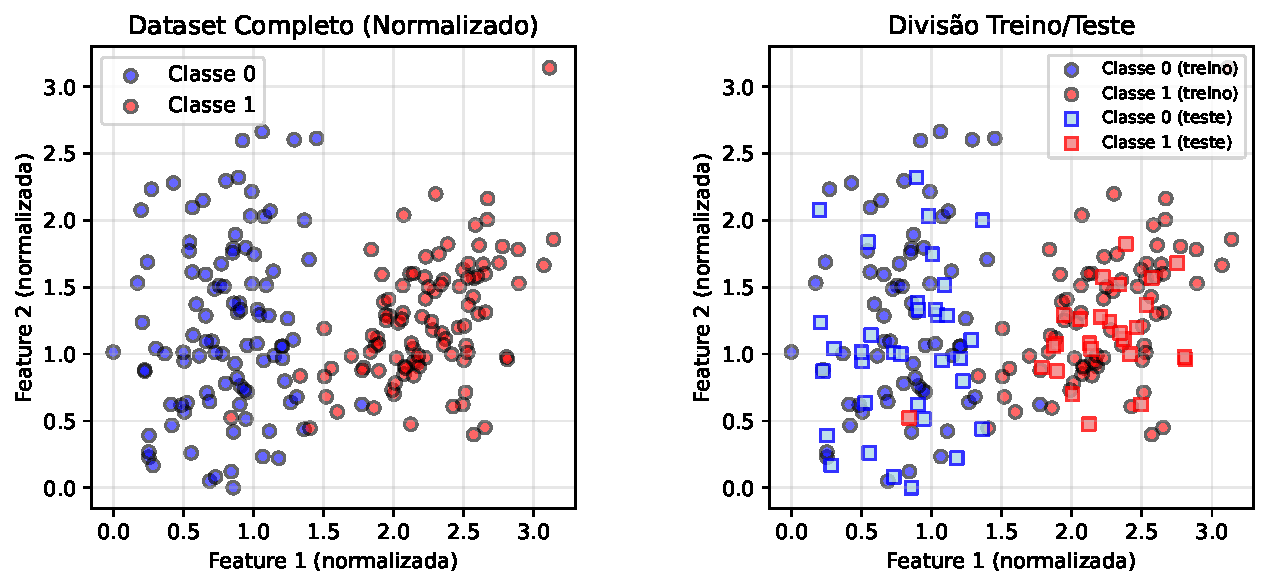
\includegraphics[keepaspectratio]{apostila_files/figure-pdf/cell-146-output-1.pdf}}

\begin{verbatim}
Total de amostras: 200
Amostras de treino: 140 (70.0%)
Amostras de teste: 60 (30.0%)
Distribuição de classes: Classe 0: 100, Classe 1: 100
\end{verbatim}

\begin{verbatim}
Total de amostras: 200
Amostras de treino: 140 (70.0%)
Amostras de teste: 60 (30.0%)
Distribuição de classes: Classe 0: 100, Classe 1: 100
\end{verbatim}

\subsection{2.1 O Feature Map: A Ponte Entre os Mundos Clássico e
Quântico}\label{o-feature-map-a-ponte-entre-os-mundos-cluxe1ssico-e-quuxe2ntico}

\subsubsection{🌉 O que é um Feature
Map?}\label{o-que-uxe9-um-feature-map}

Em Machine Learning clássico, seus dados são simplesmente números em um
vetor (por exemplo, \texttt{{[}1.2,\ 3.4{]}}). Mas um computador
quântico não entende números diretamente - ele trabalha com
\textbf{estados quânticos} (superposições e emaranhamentos de qubits).

O \textbf{Feature Map} é a função que realiza essa tradução:

\begin{verbatim}
Dados Clássicos (x₁, x₂, ..., xₙ)  →  |ψ(x)⟩ Estado Quântico
\end{verbatim}

\textbf{Analogia:} Pense no Feature Map como um ``tradutor universal''.
Se você quer comunicar com alienígenas (qubits), precisa converter seu
idioma (números) para o idioma deles (estados quânticos).

\subsubsection{🔬 Por que precisamos
disso?}\label{por-que-precisamos-disso}

\begin{enumerate}
\def\labelenumi{\arabic{enumi}.}
\tightlist
\item
  \textbf{Interface de Comunicação:} Qubits não ``leem'' números
  diretamente. Eles existem em superposições de \textbar0⟩ e \textbar1⟩
\item
  \textbf{Projeção em Alta Dimensão:} Um Feature Map quântico projeta
  seus dados n-dimensionais em um espaço de \textbf{2ⁿ dimensões} (o
  espaço de Hilbert). Isso é exponencialmente maior!
\item
  \textbf{Separação Não-Linear:} Problemas que são difíceis de separar
  no espaço original podem se tornar triviais no espaço quântico de alta
  dimensão
\end{enumerate}

\subsubsection{⚡ O ZZFeatureMap
Especificamente}\label{o-zzfeaturemap-especificamente}

O \texttt{ZZFeatureMap} é um dos Feature Maps mais populares em QML. O
nome vem das \textbf{portas ZZ} (interações entre qubits usando operador
Pauli-Z).

\textbf{Estrutura do ZZFeatureMap:}

\begin{enumerate}
\def\labelenumi{\arabic{enumi}.}
\item
  \textbf{Camada de Hadamard (H):}

\begin{verbatim}
H|0⟩ → (|0⟩ + |1⟩)/√2
\end{verbatim}

  Coloca todos os qubits em superposição uniforme (ponto de partida
  neutro)
\item
  \textbf{Codificação Individual (Rotações RZ):}

\begin{verbatim}
RZ(xᵢ)|ψ⟩
\end{verbatim}

  Cada feature \texttt{xᵢ} dos seus dados gira o qubit correspondente em
  torno do eixo Z por \texttt{xᵢ} radianos
\item
  \textbf{Interações ZZ (Emaranhamento):}

\begin{verbatim}
ZZ(xᵢ · xⱼ) = exp(-i · xᵢ · xⱼ · Z ⊗ Z)
\end{verbatim}

  Cria correlações não-lineares entre diferentes features através do
  \textbf{produto} \texttt{xᵢ\ ·\ xⱼ}
\item
  \textbf{Repetições (reps):} Todo o processo (H + RZ + ZZ) pode ser
  repetido múltiplas vezes para aumentar a expressividade
\end{enumerate}

\subsubsection{🎯 Exemplo Concreto}\label{exemplo-concreto}

Suponha que você tem dados \texttt{x\ =\ {[}0.5,\ 1.2{]}} (2 features) e
quer usar um ZZFeatureMap com 2 qubits:

\begin{verbatim}
Estado Inicial: |00⟩

1. Aplicar Hadamard:
   H⊗H|00⟩ → (|00⟩ + |01⟩ + |10⟩ + |11⟩)/2

2. Codificar Feature 1 (x₁ = 0.5):
   RZ(0.5) no qubit 0

3. Codificar Feature 2 (x₂ = 1.2):
   RZ(1.2) no qubit 1

4. Criar Interação ZZ:
   ZZ(0.5 × 1.2 = 0.6) entre qubits 0 e 1
   Isso emaranha os qubits proporcionalmente ao produto das features!

5. (Opcional) Repetir para reps > 1
\end{verbatim}

O estado final \texttt{\textbar{}ψ(x)⟩} agora codifica seus dados em um
espaço de \textbf{2² = 4 dimensões}.

\subsubsection{💡 Por que o produto xᵢ · xⱼ é
importante?}\label{por-que-o-produto-xux1d62-xux2c7c-uxe9-importante}

A interação \textbf{ZZ} usa o \textbf{produto} das features, não a soma.
Isso cria \textbf{termos não-lineares} que são cruciais para:

\begin{itemize}
\tightlist
\item
  Capturar correlações entre variáveis (por exemplo, ``altura × peso'')
\item
  Resolver problemas que não são linearmente separáveis
\item
  Implementar um kernel quântico de alta expressividade
\end{itemize}

\textbf{Comparação:} - \textbf{Feature Map Linear:} φ(x) = {[}x₁, x₂{]}
→ 2D - \textbf{Kernel Polinomial (clássico):} φ(x) = {[}x₁, x₂, x₁²,
x₂², x₁·x₂{]} → 5D - \textbf{ZZFeatureMap (quântico):} φ(x) =
\textbar ψ(x)⟩ → 2ⁿ dimensional (exponencial!)

\subsubsection{🔢 Parâmetros
Importantes}\label{paruxe2metros-importantes}

Quando criamos \texttt{ZZFeatureMap(feature\_dimension=2,\ reps=1)}:

\begin{itemize}
\tightlist
\item
  \texttt{feature\_dimension=2}: Número de features de entrada
  (determina número de qubits)
\item
  \texttt{reps=1}: Quantas vezes repetir a sequência H → RZ → ZZ

  \begin{itemize}
  \tightlist
  \item
    \texttt{reps=1}: Circuito raso, rápido, menos expressivo
  \item
    \texttt{reps=2}: Mais profundo, mais expressivo, mas mais lento
  \item
    \texttt{reps≥3}: Máxima expressividade, mas risco de overfitting e
    lentidão
  \end{itemize}
\end{itemize}

\subsubsection{🌟 Vantagens do
ZZFeatureMap}\label{vantagens-do-zzfeaturemap}

✅ \textbf{Emaranhamento Nativo:} Cria correlações quânticas
automaticamente\\
✅ \textbf{Não-Linearidade:} Termos xᵢ·xⱼ sem custo computacional
extra\\
✅ \textbf{Escalável:} Funciona bem para 2-10 qubits (na era NISQ
atual)\\
✅ \textbf{Compatível:} Amplamente suportado em Qiskit e hardware IBM

\subsubsection{⚠️ Limitações e
Considerações}\label{limitauxe7uxf5es-e-considerauxe7uxf5es}

\begin{itemize}
\tightlist
\item
  \textbf{Normalização Crítica:} Features devem estar em {[}0, π{]} ou
  {[}-π, π{]}, caso contrário as rotações perdem significado
\item
  \textbf{Ruído:} Circuitos profundos (reps alto) acumulam mais ruído em
  hardware real
\item
  \textbf{Barren Plateaus:} Em circuitos muito profundos, gradientes
  podem ``desaparecer'', dificultando treinamento
\end{itemize}

\subsubsection{📊 Alternativas ao
ZZFeatureMap}\label{alternativas-ao-zzfeaturemap}

Outros Feature Maps populares:

\begin{longtable}[]{@{}
  >{\raggedright\arraybackslash}p{(\linewidth - 2\tabcolsep) * \real{0.4286}}
  >{\raggedright\arraybackslash}p{(\linewidth - 2\tabcolsep) * \real{0.5714}}@{}}
\toprule\noalign{}
\begin{minipage}[b]{\linewidth}\raggedright
Feature Map
\end{minipage} & \begin{minipage}[b]{\linewidth}\raggedright
Características
\end{minipage} \\
\midrule\noalign{}
\endhead
\bottomrule\noalign{}
\endlastfoot
\textbf{PauliFeatureMap} & Usa rotações X, Y, Z (mais geral) \\
\textbf{StatePreparation} & Codifica amplitudes diretamente (custoso) \\
\textbf{Custom Feature Map} & Você desenha o circuito (máxima
flexibilidade) \\
\end{longtable}

O \textbf{ZZFeatureMap} é um ótimo ponto de partida: equilibra
expressividade e eficiência!

\subsubsection{🔍 Visualização Mental}\label{visualizauxe7uxe3o-mental}

\begin{verbatim}
┌─────────────────────────────────────────┐
│  MUNDO CLÁSSICO                         │
│  Dados: x = [0.5, 1.2]                  │
│         (2 dimensões)                   │
└──────────────┬──────────────────────────┘
               │
               │ ZZFeatureMap
               │ (Tradução)
               ▼
┌─────────────────────────────────────────┐
│  MUNDO QUÂNTICO                         │
│  Estado: |ψ(x)⟩ = α₀₀|00⟩ + α₀₁|01⟩   │
│                + α₁₀|10⟩ + α₁₁|11⟩    │
│         (4 dimensões complexas!)       │
│  Com emaranhamento e correlações!      │
└─────────────────────────────────────────┘
\end{verbatim}

\textbf{Resumo:} O Feature Map é a ``rampa de acesso'' ao mundo
quântico, e o ZZFeatureMap faz isso de forma eficiente usando
emaranhamento ZZ para capturar interações não-lineares entre suas
features!

\begin{Shaded}
\begin{Highlighting}[]
\CommentTok{\# {-}{-}{-} 2. O FEATURE MAP (Tradutor Dados {-}\textgreater{} Quantum) {-}{-}{-}}
\CommentTok{\# ZZFeatureMap é famoso por criar emaranhamento entre os dados,}
\CommentTok{\# ajudando a resolver problemas não{-}lineares.}
\NormalTok{num\_qubits }\OperatorTok{=} \DecValTok{2}
\NormalTok{feature\_map }\OperatorTok{=}\NormalTok{ ZZFeatureMap(feature\_dimension}\OperatorTok{=}\NormalTok{num\_qubits, reps}\OperatorTok{=}\DecValTok{1}\NormalTok{)}
\end{Highlighting}
\end{Shaded}

\begin{verbatim}
/tmp/ipykernel_666762/1824718266.py:5: DeprecationWarning: The class ``qiskit.circuit.library.data_preparation._zz_feature_map.ZZFeatureMap`` is deprecated as of Qiskit 2.1. It will be removed in Qiskit 3.0. Use the zz_feature_map function as a replacement. Note that this will no longer return a BlueprintCircuit, but just a plain QuantumCircuit.
  feature_map = ZZFeatureMap(feature_dimension=num_qubits, reps=1)
\end{verbatim}

\begin{verbatim}
C:\Users\Max\AppData\Local\Temp\ipykernel_20596\1784461025.py:5: DeprecationWarning: The class ``qiskit.circuit.library.data_preparation._zz_feature_map.ZZFeatureMap`` is deprecated as of Qiskit 2.1. It will be removed in Qiskit 3.0. Use the zz_feature_map function as a replacement. Note that this will no longer return a BlueprintCircuit, but just a plain QuantumCircuit.
  feature_map = ZZFeatureMap(feature_dimension=num_qubits, reps=1)
\end{verbatim}

\subsubsection{Visualizando o Feature
Map}\label{visualizando-o-feature-map}

O \textbf{Feature Map} é a ``ponte'' entre o mundo clássico e o
quântico. Vamos visualizar o circuito:

\begin{Shaded}
\begin{Highlighting}[]
\CommentTok{\# Visualizar o Feature Map com dados reais}
\BuiltInTok{print}\NormalTok{(}\StringTok{"Feature Map {-} Circuito de Codificação dos Dados"}\NormalTok{)}
\BuiltInTok{print}\NormalTok{(}\StringTok{"="} \OperatorTok{*} \DecValTok{60}\NormalTok{)}
\BuiltInTok{print}\NormalTok{(}\SpecialStringTok{f"Número de qubits: }\SpecialCharTok{\{}\NormalTok{num\_qubits}\SpecialCharTok{\}}\SpecialStringTok{"}\NormalTok{)}
\BuiltInTok{print}\NormalTok{(}\SpecialStringTok{f"Número de repetições: }\SpecialCharTok{\{}\NormalTok{feature\_map}\SpecialCharTok{.}\NormalTok{reps}\SpecialCharTok{\}}\SpecialStringTok{"}\NormalTok{)}
\BuiltInTok{print}\NormalTok{(}\SpecialStringTok{f"Dimensão das features: }\SpecialCharTok{\{}\NormalTok{feature\_map}\SpecialCharTok{.}\NormalTok{feature\_dimension}\SpecialCharTok{\}}\SpecialStringTok{"}\NormalTok{)}
\BuiltInTok{print}\NormalTok{()}

\CommentTok{\# Criar uma instância do feature map com dados de exemplo}
\NormalTok{sample\_data }\OperatorTok{=}\NormalTok{ X\_train[}\DecValTok{0}\NormalTok{]  }\CommentTok{\# Pegar a primeira amostra}
\BuiltInTok{print}\NormalTok{(}\SpecialStringTok{f"Exemplo de dados de entrada: }\SpecialCharTok{\{}\NormalTok{sample\_data}\SpecialCharTok{\}}\SpecialStringTok{"}\NormalTok{)}
\BuiltInTok{print}\NormalTok{(}\SpecialStringTok{f"  Feature 1: }\SpecialCharTok{\{}\NormalTok{sample\_data[}\DecValTok{0}\NormalTok{]}\SpecialCharTok{:.4f\}}\SpecialStringTok{ radianos"}\NormalTok{)}
\BuiltInTok{print}\NormalTok{(}\SpecialStringTok{f"  Feature 2: }\SpecialCharTok{\{}\NormalTok{sample\_data[}\DecValTok{1}\NormalTok{]}\SpecialCharTok{:.4f\}}\SpecialStringTok{ radianos"}\NormalTok{)}
\BuiltInTok{print}\NormalTok{()}

\CommentTok{\# Bind dos parâmetros com dados reais}
\NormalTok{feature\_map\_bound }\OperatorTok{=}\NormalTok{ feature\_map.assign\_parameters(sample\_data)}
\BuiltInTok{print}\NormalTok{(}\StringTok{"Circuito com parâmetros atribuídos:"}\NormalTok{)}
\NormalTok{display(feature\_map\_bound.decompose().draw(output}\OperatorTok{=}\StringTok{\textquotesingle{}mpl\textquotesingle{}}\NormalTok{, idle\_wires}\OperatorTok{=}\VariableTok{False}\NormalTok{, scale}\OperatorTok{=}\FloatTok{0.8}\NormalTok{))}
\end{Highlighting}
\end{Shaded}

\begin{verbatim}
Feature Map - Circuito de Codificação dos Dados
============================================================
Número de qubits: 2
Número de repetições: 1
Dimensão das features: 2

Exemplo de dados de entrada: [2.32325348 1.74815771]
  Feature 1: 2.3233 radianos
  Feature 2: 1.7482 radianos

Circuito com parâmetros atribuídos:
\end{verbatim}

\pandocbounded{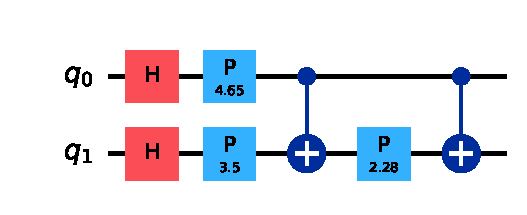
\includegraphics[keepaspectratio]{apostila_files/figure-pdf/cell-148-output-2.pdf}}

\pandocbounded{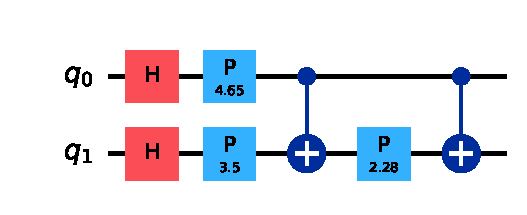
\includegraphics[keepaspectratio]{apostila_files/figure-pdf/cell-148-output-3.pdf}}

\begin{verbatim}
Feature Map - Circuito de Codificação dos Dados
============================================================
Número de qubits: 2
Número de repetições: 1
Dimensão das features: 2

Exemplo de dados de entrada: [2.32325348 1.74815771]
  Feature 1: 2.3233 radianos
  Feature 2: 1.7482 radianos

Circuito com parâmetros atribuídos:
\end{verbatim}

\subsection{2.2 O Ansatz: O ``Cérebro'' Treinável do Circuito
Quântico}\label{o-ansatz-o-cuxe9rebro-treinuxe1vel-do-circuito-quuxe2ntico}

\subsubsection{🧠 O que é um Ansatz?}\label{o-que-uxe9-um-ansatz}

Enquanto o \textbf{Feature Map} codifica os dados de entrada, o
\textbf{Ansatz} é onde o ``aprendizado'' acontece. É o circuito quântico
parametrizado cujos ângulos de rotação (θ) são ajustados durante o
treinamento.

\textbf{Analogia com Redes Neurais Clássicas:}

\begin{verbatim}
Rede Neural Clássica:
Input → [W₁, b₁] → Hidden Layer → [W₂, b₂] → Output
         ↑ pesos treináveis ↑

VQC Quântico:
|ψ(x)⟩ → [θ₁, θ₂, θ₃, ...] → Ansatz → Medição
          ↑ ângulos treináveis ↑
\end{verbatim}

O \textbf{Ansatz} é literalmente a ``rede neural quântica'' - um
template de circuito com parâmetros que serão otimizados para minimizar
o erro de classificação.

\subsubsection{🎯 O Nome ``Ansatz''}\label{o-nome-ansatz}

\textbf{Etimologia:} Do alemão \emph{Ansatz} = ``abordagem inicial'' ou
``proposta''

Em física e matemática, um \emph{ansatz} é uma suposição educada sobre a
forma da solução de um problema. No QML: - Você \textbf{propõe} uma
estrutura de circuito (RY rotations + CX gates) - O otimizador
\textbf{ajusta} os parâmetros θ para encontrar a melhor solução - É uma
``tentativa estruturada'' de encontrar o circuito ideal

\subsubsection{⚡ O RealAmplitudes
Especificamente}\label{o-realamplitudes-especificamente}

O \texttt{RealAmplitudes} é um dos ansatz mais populares e eficientes em
QML. O nome vem do fato de que ele manipula apenas \textbf{amplitudes
reais} (não usa números complexos de fase arbitrária).

\textbf{Estrutura do RealAmplitudes:}

\begin{enumerate}
\def\labelenumi{\arabic{enumi}.}
\item
  \textbf{Camada de Rotação (RY gates):}

\begin{verbatim}
RY(θᵢ)|ψ⟩ = cos(θᵢ/2)|0⟩ + sin(θᵢ/2)|1⟩
\end{verbatim}

  Cada qubit recebe uma rotação RY com ângulo θ treinável. A porta RY
  gira o qubit no plano Y-Z da esfera de Bloch.
\item
  \textbf{Camada de Emaranhamento (CX gates):}

\begin{verbatim}
CX|control⟩|target⟩
\end{verbatim}

  Portas CNOT conectam qubits vizinhos, criando emaranhamento
  (correlações quânticas entre qubits)
\item
  \textbf{Repetições (reps):} As camadas RY → CX podem ser repetidas
  múltiplas vezes, criando um circuito mais profundo e expressivo
\end{enumerate}

\textbf{Padrão típico para 2 qubits, reps=2:}

\begin{verbatim}
q[0]: ─RY(θ₀)─●───RY(θ₂)─●───
              │           │
q[1]: ─RY(θ₁)─X───RY(θ₃)─X───
\end{verbatim}

\subsubsection{🔬 Exemplo Detalhado: RealAmplitudes(num\_qubits=2,
reps=1)}\label{exemplo-detalhado-realamplitudesnum_qubits2-reps1}

\textbf{Estrutura:} 1. \textbf{Primeira camada de rotação:} -
\texttt{RY(θ₀)} no qubit 0 - \texttt{RY(θ₁)} no qubit 1

\begin{enumerate}
\def\labelenumi{\arabic{enumi}.}
\setcounter{enumi}{1}
\tightlist
\item
  \textbf{Camada de emaranhamento:}

  \begin{itemize}
  \tightlist
  \item
    \texttt{CX(qubit\ 0\ →\ qubit\ 1)} - qubit 0 controla qubit 1
  \end{itemize}
\item
  \textbf{Segunda camada de rotação:}

  \begin{itemize}
  \tightlist
  \item
    \texttt{RY(θ₂)} no qubit 0
  \item
    \texttt{RY(θ₃)} no qubit 1
  \end{itemize}
\end{enumerate}

\textbf{Total:} 4 parâmetros treináveis (θ₀, θ₁, θ₂, θ₃)

\textbf{Durante o treinamento:} - O otimizador testa diferentes
combinações de ângulos - Por exemplo: θ = {[}0.5, 1.2, 0.8, 2.1{]} -
Avalia o erro de classificação - Ajusta os ângulos para reduzir o erro -
Repete até convergir!

\subsubsection{💡 Por que Rotações RY?}\label{por-que-rotauxe7uxf5es-ry}

A porta \textbf{RY} foi escolhida porque:

\begin{enumerate}
\def\labelenumi{\arabic{enumi}.}
\item
  \textbf{Amplitudes Reais:} RY(θ)\textbar0⟩ = cos(θ/2)\textbar0⟩ +
  sin(θ/2)\textbar1⟩

  \begin{itemize}
  \tightlist
  \item
    Os coeficientes são reais (não complexos)
  \item
    Simplifica cálculos e otimização
  \end{itemize}
\item
  \textbf{Cobertura Completa:} Com RY + emaranhamento, você pode
  alcançar qualquer estado quântico necessário
\item
  \textbf{Eficiência:} Menos portas = menos ruído em hardware real
\item
  \textbf{Expressividade:} Mesmo sendo simples, é surpreendentemente
  poderoso para ML
\end{enumerate}

\textbf{Comparação com outras rotações:} - \textbf{RZ(θ):} Adiciona
apenas fase (não muda probabilidades diretamente) - \textbf{RX(θ):}
Similar ao RY, mas em eixo diferente - \textbf{RY(θ):} Ideal - muda
amplitudes diretamente sem fase extra

\subsubsection{🔢 Calculando o Número de
Parâmetros}\label{calculando-o-nuxfamero-de-paruxe2metros}

\textbf{Fórmula para RealAmplitudes:}

\begin{verbatim}
num_params = num_qubits × (reps + 1)
\end{verbatim}

\textbf{Exemplos:} - \texttt{RealAmplitudes(2\ qubits,\ reps=1)}: 2 ×
(1+1) = \textbf{4 parâmetros} -
\texttt{RealAmplitudes(2\ qubits,\ reps=2)}: 2 × (2+1) = \textbf{6
parâmetros} - \texttt{RealAmplitudes(2\ qubits,\ reps=3)}: 2 × (3+1) =
\textbf{8 parâmetros} - \texttt{RealAmplitudes(4\ qubits,\ reps=2)}: 4 ×
(2+1) = \textbf{12 parâmetros}

\textbf{Trade-off:} - ✅ Mais parâmetros = maior expressividade = pode
aprender padrões complexos - ⚠️ Mais parâmetros = mais lento para
otimizar = risco de overfitting

\subsubsection{🎨 Visualização: Como o Ansatz Transforma
Estados}\label{visualizauxe7uxe3o-como-o-ansatz-transforma-estados}

Imagine que o Feature Map criou o estado inicial
\texttt{\textbar{}ψ(x)⟩} para seus dados.

\textbf{O Ansatz então:}

\begin{verbatim}
Estado Inicial (do Feature Map):
|ψ(x)⟩ = α₀₀|00⟩ + α₀₁|01⟩ + α₁₀|10⟩ + α₁₁|11⟩

↓ Aplicar RY(θ₀) e RY(θ₁)

Estado após rotações individuais:
Cada qubit é rotado, mudando as amplitudes

↓ Aplicar CX (emaranhamento)

Estado emaranhado:
Qubits agora correlacionados - não podem ser descritos separadamente!

↓ Aplicar RY(θ₂) e RY(θ₃)

Estado final preparado para medição:
|ψ_final⟩ com amplitudes ajustadas para classificação
\end{verbatim}

\textbf{Medição final:} - Se medir mais \textbar0⟩: Predição = Classe 0
- Se medir mais \textbar1⟩: Predição = Classe 1

\subsubsection{🔄 O Processo de Treinamento
(Otimização)}\label{o-processo-de-treinamento-otimizauxe7uxe3o}

\textbf{Objetivo:} Encontrar θ* que minimiza a função de perda

\begin{Shaded}
\begin{Highlighting}[]
\FloatTok{1.}\NormalTok{ Inicializar θ aleatoriamente}
\FloatTok{2.}\NormalTok{ Para cada iteração:}
\NormalTok{   a. Executar circuito: Feature Map → Ansatz(θ) → Medição}
\NormalTok{   b. Calcular predições com base nas medições}
\NormalTok{   c. Calcular erro (cross}\OperatorTok{{-}}\NormalTok{entropy loss)}
\NormalTok{   d. Ajustar θ para reduzir erro (via COBYLA ou outro otimizador)}
\FloatTok{3.}\NormalTok{ Retornar θ}\OperatorTok{*}\NormalTok{ otimizado}
\end{Highlighting}
\end{Shaded}

\textbf{Otimizador COBYLA:} - Constrained Optimization BY Linear
Approximations - Não usa gradientes (bom para simuladores ruidosos) -
Testa pequenas variações em θ e escolhe a melhor direção - Iterativo -
pode levar 100-500 iterações para convergir

\subsubsection{🌟 Vantagens do
RealAmplitudes}\label{vantagens-do-realamplitudes}

✅ \textbf{Simplicidade:} Fácil de entender e implementar\\
✅ \textbf{Eficiência:} Poucas portas = menos ruído\\
✅ \textbf{Expressividade:} Surpreendentemente poderoso para
classificação\\
✅ \textbf{Escalável:} Funciona bem com 2-10 qubits (era NISQ)\\
✅ \textbf{Bem Testado:} Amplamente usado em papers e aplicações

\subsubsection{⚠️ Limitações e
Considerações}\label{limitauxe7uxf5es-e-considerauxe7uxf5es-1}

\textbf{Barren Plateaus:} - Em circuitos muito profundos (reps alto),
gradientes podem ``desaparecer'' - Otimização fica presa em platôs
planos onde todos θ parecem igualmente ruins - \textbf{Solução:} Use
reps moderado (1-3), ou otimizadores especializados

\textbf{Overfitting:} - Muitos parâmetros podem memorizar dados de
treino - \textbf{Solução:} Regularização, validação cruzada, ou reps
menor

\textbf{Inicialização:} - θ inicial aleatório pode levar a mínimos
locais ruins - \textbf{Solução:} Tentar múltiplas inicializações ou usar
inicialização informada

\subsubsection{📊 Alternativas ao
RealAmplitudes}\label{alternativas-ao-realamplitudes}

Outros ansatz populares:

\begin{longtable}[]{@{}
  >{\raggedright\arraybackslash}p{(\linewidth - 2\tabcolsep) * \real{0.3333}}
  >{\raggedright\arraybackslash}p{(\linewidth - 2\tabcolsep) * \real{0.6667}}@{}}
\toprule\noalign{}
\begin{minipage}[b]{\linewidth}\raggedright
Ansatz
\end{minipage} & \begin{minipage}[b]{\linewidth}\raggedright
Características
\end{minipage} \\
\midrule\noalign{}
\endhead
\bottomrule\noalign{}
\endlastfoot
\textbf{EfficientSU2} & Usa RY + RZ (mais geral, mais parâmetros) \\
\textbf{TwoLocal} & Template customizável (você escolhe portas) \\
\textbf{ExcitationPreserving} & Preserva número de excitações (para
química) \\
\textbf{Hardware Efficient} & Otimizado para topologia específica de
hardware \\
\end{longtable}

O \textbf{RealAmplitudes} é ótimo para começar: simples, eficiente e
funciona!

\subsubsection{🔍 Comparação: Feature Map vs
Ansatz}\label{comparauxe7uxe3o-feature-map-vs-ansatz}

\begin{longtable}[]{@{}lll@{}}
\toprule\noalign{}
Aspecto & \textbf{Feature Map} & \textbf{Ansatz} \\
\midrule\noalign{}
\endhead
\bottomrule\noalign{}
\endlastfoot
\textbf{Função} & Codificar dados & Aprender padrões \\
\textbf{Parâmetros} & Valores dos dados (x) & Pesos treináveis (θ) \\
\textbf{Treinamento} & Fixo (não muda) & Otimizado \\
\textbf{Analogia ML} & Camada de entrada & Camadas ocultas \\
\textbf{Exemplo} & ZZFeatureMap & RealAmplitudes \\
\textbf{Portas Típicas} & H, RZ, ZZ & RY, CX \\
\end{longtable}

\textbf{Juntos formam o VQC:}

\begin{verbatim}
Dados → Feature Map → Ansatz → Medição → Predição
  x        |ψ(x)⟩        θ      |0⟩ ou |1⟩    classe
\end{verbatim}

\subsubsection{🎓 Conceito-Chave:
Expressividade}\label{conceito-chave-expressividade}

\textbf{Expressividade} = capacidade do Ansatz de representar diferentes
funções

\textbf{Fatores que aumentam expressividade:} 1. Mais qubits (espaço
maior) 2. Mais repetições (circuito mais profundo) 3. Mais tipos de
portas (RX, RY, RZ combinados) 4. Padrões de emaranhamento mais
complexos

\textbf{Regra de Ouro:} - Para problemas simples: \texttt{reps=1-2} é
suficiente - Para problemas complexos: \texttt{reps=3-5} pode ajudar -
Além disso: diminishing returns + mais ruído

\subsubsection{💻 Exemplo de Código
Customizado}\label{exemplo-de-cuxf3digo-customizado}

Se quiser criar seu próprio ansatz:

\begin{Shaded}
\begin{Highlighting}[]
\ImportTok{from}\NormalTok{ qiskit.circuit }\ImportTok{import}\NormalTok{ QuantumCircuit, Parameter}

\CommentTok{\# Criar ansatz customizado}
\NormalTok{num\_qubits }\OperatorTok{=} \DecValTok{2}
\NormalTok{theta }\OperatorTok{=}\NormalTok{ [Parameter(}\SpecialStringTok{f\textquotesingle{}θ}\SpecialCharTok{\{}\NormalTok{i}\SpecialCharTok{\}}\SpecialStringTok{\textquotesingle{}}\NormalTok{) }\ControlFlowTok{for}\NormalTok{ i }\KeywordTok{in} \BuiltInTok{range}\NormalTok{(}\DecValTok{6}\NormalTok{)]}

\NormalTok{custom\_ansatz }\OperatorTok{=}\NormalTok{ QuantumCircuit(num\_qubits)}

\CommentTok{\# Camada 1}
\NormalTok{custom\_ansatz.ry(theta[}\DecValTok{0}\NormalTok{], }\DecValTok{0}\NormalTok{)}
\NormalTok{custom\_ansatz.ry(theta[}\DecValTok{1}\NormalTok{], }\DecValTok{1}\NormalTok{)}
\NormalTok{custom\_ansatz.cx(}\DecValTok{0}\NormalTok{, }\DecValTok{1}\NormalTok{)}

\CommentTok{\# Camada 2}
\NormalTok{custom\_ansatz.ry(theta[}\DecValTok{2}\NormalTok{], }\DecValTok{0}\NormalTok{)}
\NormalTok{custom\_ansatz.ry(theta[}\DecValTok{3}\NormalTok{], }\DecValTok{1}\NormalTok{)}
\NormalTok{custom\_ansatz.cx(}\DecValTok{1}\NormalTok{, }\DecValTok{0}\NormalTok{)  }\CommentTok{\# Direção diferente!}

\CommentTok{\# Camada 3}
\NormalTok{custom\_ansatz.ry(theta[}\DecValTok{4}\NormalTok{], }\DecValTok{0}\NormalTok{)}
\NormalTok{custom\_ansatz.ry(theta[}\DecValTok{5}\NormalTok{], }\DecValTok{1}\NormalTok{)}
\end{Highlighting}
\end{Shaded}

Isso dá controle total sobre a arquitetura!

\subsubsection{🔬 Resumo Visual}\label{resumo-visual}

\begin{verbatim}
┌─────────────────────────────────────────────────┐
│  ANSATZ = "Rede Neural Quântica"                │
│                                                 │
│  Entrada: |ψ(x)⟩ (do Feature Map)              │
│     ↓                                           │
│  [ RY(θ₀) RY(θ₁) ]  ← Parâmetros treináveis    │
│     ↓                                           │
│  [ CX gate ]  ← Emaranhamento                  │
│     ↓                                           │
│  [ RY(θ₂) RY(θ₃) ]  ← Mais parâmetros          │
│     ↓                                           │
│  Saída: Estado preparado para medição          │
│                                                 │
│  O Otimizador ajusta θ para minimizar erro!    │
└─────────────────────────────────────────────────┘
\end{verbatim}

\textbf{Resumo em uma frase:} O Ansatz é o circuito parametrizado que
``aprende'' a classificar dados ajustando ângulos de rotação θ,
exatamente como uma rede neural clássica ajusta pesos W!

\begin{Shaded}
\begin{Highlighting}[]
\CommentTok{\# {-}{-}{-} 3. O ANSATZ (O Modelo Treinável) {-}{-}{-}}
\CommentTok{\# RealAmplitudes é um circuito simples com rotações RY e emaranhamento.}
\CommentTok{\# É a nossa "Rede Neural".}
\NormalTok{ansatz }\OperatorTok{=}\NormalTok{ RealAmplitudes(num\_qubits}\OperatorTok{=}\NormalTok{num\_qubits, reps}\OperatorTok{=}\DecValTok{1}\NormalTok{)}
\end{Highlighting}
\end{Shaded}

\begin{verbatim}
/tmp/ipykernel_666762/4274500007.py:4: DeprecationWarning: The class ``qiskit.circuit.library.n_local.real_amplitudes.RealAmplitudes`` is deprecated as of Qiskit 2.1. It will be removed in Qiskit 3.0. Use the function qiskit.circuit.library.real_amplitudes instead.
  ansatz = RealAmplitudes(num_qubits=num_qubits, reps=1)
\end{verbatim}

\begin{verbatim}
C:\Users\Max\AppData\Local\Temp\ipykernel_20596\2137702756.py:4: DeprecationWarning: The class ``qiskit.circuit.library.n_local.real_amplitudes.RealAmplitudes`` is deprecated as of Qiskit 2.1. It will be removed in Qiskit 3.0. Use the function qiskit.circuit.library.real_amplitudes instead.
  ansatz = RealAmplitudes(num_qubits=num_qubits, reps=1)
\end{verbatim}

\subsubsection{Visualizando o Ansatz}\label{visualizando-o-ansatz}

O \textbf{Ansatz} é o ``modelo treinável'' - equivalente aos pesos de
uma rede neural clássica:

\begin{Shaded}
\begin{Highlighting}[]
\CommentTok{\# Visualizar o Ansatz}
\BuiltInTok{print}\NormalTok{(}\StringTok{"Ansatz {-} Modelo Treinável (Rede Neural Quântica)"}\NormalTok{)}
\BuiltInTok{print}\NormalTok{(}\StringTok{"="} \OperatorTok{*} \DecValTok{60}\NormalTok{)}
\BuiltInTok{print}\NormalTok{(}\SpecialStringTok{f"Número de qubits: }\SpecialCharTok{\{}\NormalTok{ansatz}\SpecialCharTok{.}\NormalTok{num\_qubits}\SpecialCharTok{\}}\SpecialStringTok{"}\NormalTok{)}
\BuiltInTok{print}\NormalTok{(}\SpecialStringTok{f"Número de repetições: }\SpecialCharTok{\{}\NormalTok{ansatz}\SpecialCharTok{.}\NormalTok{reps}\SpecialCharTok{\}}\SpecialStringTok{"}\NormalTok{)}
\BuiltInTok{print}\NormalTok{(}\SpecialStringTok{f"Número de parâmetros treináveis: }\SpecialCharTok{\{}\NormalTok{ansatz}\SpecialCharTok{.}\NormalTok{num\_parameters}\SpecialCharTok{\}}\SpecialStringTok{"}\NormalTok{)}
\BuiltInTok{print}\NormalTok{()}
\BuiltInTok{print}\NormalTok{(}\StringTok{"Estes parâmetros θ são ajustados durante o treinamento,"}\NormalTok{)}
\BuiltInTok{print}\NormalTok{(}\StringTok{"assim como os pesos W em uma rede neural clássica."}\NormalTok{)}
\BuiltInTok{print}\NormalTok{()}

\NormalTok{display(ansatz.decompose().draw(output}\OperatorTok{=}\StringTok{\textquotesingle{}mpl\textquotesingle{}}\NormalTok{, idle\_wires}\OperatorTok{=}\VariableTok{False}\NormalTok{, scale}\OperatorTok{=}\FloatTok{0.8}\NormalTok{))}
\end{Highlighting}
\end{Shaded}

\begin{verbatim}
Ansatz - Modelo Treinável (Rede Neural Quântica)
============================================================
Número de qubits: 2
Número de repetições: 1
Número de parâmetros treináveis: 4

Estes parâmetros θ são ajustados durante o treinamento,
assim como os pesos W em uma rede neural clássica.
\end{verbatim}

\pandocbounded{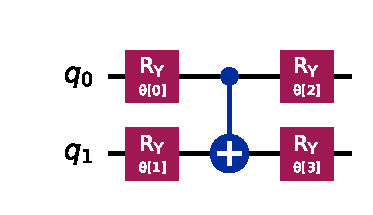
\includegraphics[keepaspectratio]{apostila_files/figure-pdf/cell-150-output-2.pdf}}

\pandocbounded{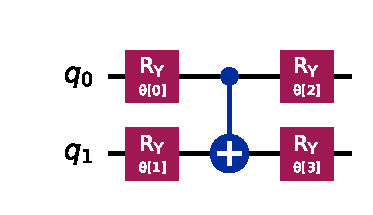
\includegraphics[keepaspectratio]{apostila_files/figure-pdf/cell-150-output-3.pdf}}

\begin{verbatim}
Ansatz - Modelo Treinável (Rede Neural Quântica)
============================================================
Número de qubits: 2
Número de repetições: 1
Número de parâmetros treináveis: 4

Estes parâmetros θ são ajustados durante o treinamento,
assim como os pesos W em uma rede neural clássica.
\end{verbatim}

\begin{Shaded}
\begin{Highlighting}[]
\CommentTok{\# {-}{-}{-} 4. O MODELO VQC (Variational Quantum Classifier) {-}{-}{-}}
\CommentTok{\# Aqui juntamos tudo.}
\CommentTok{\# Otimizador COBYLA é bom para simulações (não usa gradiente, apenas tenta melhorar).}
\NormalTok{vqc }\OperatorTok{=}\NormalTok{ VQC(}
\NormalTok{    feature\_map}\OperatorTok{=}\NormalTok{feature\_map,}
\NormalTok{    ansatz}\OperatorTok{=}\NormalTok{ansatz,}
\NormalTok{    optimizer}\OperatorTok{=}\NormalTok{COBYLA(maxiter}\OperatorTok{=}\DecValTok{100}\NormalTok{),}
\NormalTok{    loss}\OperatorTok{=}\StringTok{"cross\_entropy"}\NormalTok{,}
\NormalTok{)}

\BuiltInTok{print}\NormalTok{(}\StringTok{"{-}{-}{-} Iniciando Treinamento do Modelo Quântico {-}{-}{-}"}\NormalTok{)}
\CommentTok{\# O momento mágico: O otimizador clássico vai ajustar os parâmetros do Ansatz}
\CommentTok{\# baseando{-}se nas medições quânticas.}
\NormalTok{vqc.fit(X\_train, y\_train)}
\end{Highlighting}
\end{Shaded}

\begin{verbatim}
--- Iniciando Treinamento do Modelo Quântico ---
\end{verbatim}

\begin{verbatim}
<qiskit_machine_learning.algorithms.classifiers.vqc.VQC at 0x7779da95d540>
\end{verbatim}

\begin{verbatim}
No gradient function provided, creating a gradient function. If your Sampler requires transpilation, please provide a pass manager.
\end{verbatim}

\begin{verbatim}
--- Iniciando Treinamento do Modelo Quântico ---
\end{verbatim}

\begin{Shaded}
\begin{Highlighting}[]
\CommentTok{\# {-}{-}{-} 5. AVALIAÇÃO {-}{-}{-}}
\NormalTok{score\_train }\OperatorTok{=}\NormalTok{ vqc.score(X\_train, y\_train)}
\NormalTok{score\_test }\OperatorTok{=}\NormalTok{ vqc.score(X\_test, y\_test)}

\BuiltInTok{print}\NormalTok{(}\SpecialStringTok{f"}\CharTok{\textbackslash{}n}\SpecialStringTok{Acurácia no Treino: }\SpecialCharTok{\{}\NormalTok{score\_train}\SpecialCharTok{:.2f\}}\SpecialStringTok{"}\NormalTok{)}
\BuiltInTok{print}\NormalTok{(}\SpecialStringTok{f"Acurácia no Teste:  }\SpecialCharTok{\{}\NormalTok{score\_test}\SpecialCharTok{:.2f\}}\SpecialStringTok{"}\NormalTok{)}
\end{Highlighting}
\end{Shaded}

\begin{verbatim}

Acurácia no Treino: 0.55
Acurácia no Teste:  0.47
\end{verbatim}

\begin{verbatim}

Acurácia no Treino: 0.55
Acurácia no Teste:  0.47
\end{verbatim}

\subsection{⚠️ Análise de Desempenho}\label{anuxe1lise-de-desempenho}

\textbf{Observação Importante:} Se a acurácia está muito baixa
(\textless{} 0.7), o modelo não convergiu adequadamente. Isso é comum em
QML por vários motivos:

\begin{enumerate}
\def\labelenumi{\arabic{enumi}.}
\tightlist
\item
  \textbf{Otimização Limitada:} COBYLA com 100 iterações pode não ser
  suficiente
\item
  \textbf{Landscape Complexo:} A função de perda tem muitos mínimos
  locais
\item
  \textbf{Inicialização Aleatória:} Os parâmetros iniciais podem estar
  longe do ótimo
\item
  \textbf{Ansatz Inadequado:} O circuito pode não ter expressividade
  suficiente
\end{enumerate}

\textbf{Possíveis Soluções:} - Aumentar \texttt{maxiter} para 300-500 -
Usar diferentes otimizadores (SPSA, ADAM) - Aumentar \texttt{reps} no
Feature Map e Ansatz - Rodar múltiplas vezes com diferentes
inicializações

\begin{Shaded}
\begin{Highlighting}[]
\CommentTok{\# 🔧 MELHORANDO O VQC {-} Vamos tentar otimizar melhor}
\BuiltInTok{print}\NormalTok{(}\StringTok{"="}\OperatorTok{*}\DecValTok{60}\NormalTok{)}
\BuiltInTok{print}\NormalTok{(}\StringTok{"TENTATIVA DE OTIMIZAÇÃO MELHORADA"}\NormalTok{)}
\BuiltInTok{print}\NormalTok{(}\StringTok{"="}\OperatorTok{*}\DecValTok{60}\NormalTok{)}

\CommentTok{\# Versão melhorada com mais iterações e mais repetições}
\NormalTok{vqc\_improved }\OperatorTok{=}\NormalTok{ VQC(}
\NormalTok{    feature\_map}\OperatorTok{=}\NormalTok{ZZFeatureMap(feature\_dimension}\OperatorTok{=}\NormalTok{num\_qubits, reps}\OperatorTok{=}\DecValTok{2}\NormalTok{),  }\CommentTok{\# Mais repetições}
\NormalTok{    ansatz}\OperatorTok{=}\NormalTok{RealAmplitudes(num\_qubits}\OperatorTok{=}\NormalTok{num\_qubits, reps}\OperatorTok{=}\DecValTok{3}\NormalTok{),  }\CommentTok{\# Ansatz mais profundo}
\NormalTok{    optimizer}\OperatorTok{=}\NormalTok{COBYLA(maxiter}\OperatorTok{=}\DecValTok{300}\NormalTok{),  }\CommentTok{\# Mais iterações}
\NormalTok{    loss}\OperatorTok{=}\StringTok{"cross\_entropy"}\NormalTok{,}
\NormalTok{)}

\BuiltInTok{print}\NormalTok{(}\StringTok{"}\CharTok{\textbackslash{}n}\StringTok{Treinando VQC otimizado (isso pode demorar mais)..."}\NormalTok{)}
\BuiltInTok{print}\NormalTok{(}\StringTok{"{-} Feature Map com 2 repetições"}\NormalTok{)}
\BuiltInTok{print}\NormalTok{(}\StringTok{"{-} Ansatz com 3 repetições"}\NormalTok{)  }
\BuiltInTok{print}\NormalTok{(}\StringTok{"{-} COBYLA com 300 iterações"}\NormalTok{)}
\BuiltInTok{print}\NormalTok{()}

\NormalTok{vqc\_improved.fit(X\_train, y\_train)}

\CommentTok{\# Avaliar o modelo melhorado}
\NormalTok{score\_train\_improved }\OperatorTok{=}\NormalTok{ vqc\_improved.score(X\_train, y\_train)}
\NormalTok{score\_test\_improved }\OperatorTok{=}\NormalTok{ vqc\_improved.score(X\_test, y\_test)}

\BuiltInTok{print}\NormalTok{(}\SpecialStringTok{f"}\CharTok{\textbackslash{}n}\SpecialCharTok{\{}\StringTok{\textquotesingle{}=\textquotesingle{}}\OperatorTok{*}\DecValTok{60}\SpecialCharTok{\}}\SpecialStringTok{"}\NormalTok{)}
\BuiltInTok{print}\NormalTok{(}\StringTok{"COMPARAÇÃO: VQC Original vs VQC Otimizado"}\NormalTok{)}
\BuiltInTok{print}\NormalTok{(}\SpecialStringTok{f"}\SpecialCharTok{\{}\StringTok{\textquotesingle{}=\textquotesingle{}}\OperatorTok{*}\DecValTok{60}\SpecialCharTok{\}}\SpecialStringTok{"}\NormalTok{)}
\BuiltInTok{print}\NormalTok{(}\SpecialStringTok{f"}\SpecialCharTok{\{}\StringTok{\textquotesingle{}Métrica\textquotesingle{}}\SpecialCharTok{:\textless{}30\}}\SpecialStringTok{ }\SpecialCharTok{\{}\StringTok{\textquotesingle{}Original\textquotesingle{}}\SpecialCharTok{:\textless{}15\}}\SpecialStringTok{ }\SpecialCharTok{\{}\StringTok{\textquotesingle{}Otimizado\textquotesingle{}}\SpecialCharTok{:\textless{}15\}}\SpecialStringTok{"}\NormalTok{)}
\BuiltInTok{print}\NormalTok{(}\SpecialStringTok{f"}\SpecialCharTok{\{}\StringTok{\textquotesingle{}{-}\textquotesingle{}}\OperatorTok{*}\DecValTok{60}\SpecialCharTok{\}}\SpecialStringTok{"}\NormalTok{)}
\BuiltInTok{print}\NormalTok{(}\SpecialStringTok{f"}\SpecialCharTok{\{}\StringTok{\textquotesingle{}Acurácia (Treino)\textquotesingle{}}\SpecialCharTok{:\textless{}30\}}\SpecialStringTok{ }\SpecialCharTok{\{}\NormalTok{score\_train}\SpecialCharTok{:\textless{}15.4f\}}\SpecialStringTok{ }\SpecialCharTok{\{}\NormalTok{score\_train\_improved}\SpecialCharTok{:\textless{}15.4f\}}\SpecialStringTok{"}\NormalTok{)}
\BuiltInTok{print}\NormalTok{(}\SpecialStringTok{f"}\SpecialCharTok{\{}\StringTok{\textquotesingle{}Acurácia (Teste)\textquotesingle{}}\SpecialCharTok{:\textless{}30\}}\SpecialStringTok{ }\SpecialCharTok{\{}\NormalTok{score\_test}\SpecialCharTok{:\textless{}15.4f\}}\SpecialStringTok{ }\SpecialCharTok{\{}\NormalTok{score\_test\_improved}\SpecialCharTok{:\textless{}15.4f\}}\SpecialStringTok{"}\NormalTok{)}
\BuiltInTok{print}\NormalTok{(}\SpecialStringTok{f"}\SpecialCharTok{\{}\StringTok{\textquotesingle{}Iterações\textquotesingle{}}\SpecialCharTok{:\textless{}30\}}\SpecialStringTok{ }\SpecialCharTok{\{}\StringTok{\textquotesingle{}100\textquotesingle{}}\SpecialCharTok{:\textless{}15\}}\SpecialStringTok{ }\SpecialCharTok{\{}\StringTok{\textquotesingle{}300\textquotesingle{}}\SpecialCharTok{:\textless{}15\}}\SpecialStringTok{"}\NormalTok{)}
\BuiltInTok{print}\NormalTok{(}\SpecialStringTok{f"}\SpecialCharTok{\{}\StringTok{\textquotesingle{}Feature Map reps\textquotesingle{}}\SpecialCharTok{:\textless{}30\}}\SpecialStringTok{ }\SpecialCharTok{\{}\StringTok{\textquotesingle{}1\textquotesingle{}}\SpecialCharTok{:\textless{}15\}}\SpecialStringTok{ }\SpecialCharTok{\{}\StringTok{\textquotesingle{}2\textquotesingle{}}\SpecialCharTok{:\textless{}15\}}\SpecialStringTok{"}\NormalTok{)}
\BuiltInTok{print}\NormalTok{(}\SpecialStringTok{f"}\SpecialCharTok{\{}\StringTok{\textquotesingle{}Ansatz reps\textquotesingle{}}\SpecialCharTok{:\textless{}30\}}\SpecialStringTok{ }\SpecialCharTok{\{}\StringTok{\textquotesingle{}1\textquotesingle{}}\SpecialCharTok{:\textless{}15\}}\SpecialStringTok{ }\SpecialCharTok{\{}\StringTok{\textquotesingle{}3\textquotesingle{}}\SpecialCharTok{:\textless{}15\}}\SpecialStringTok{"}\NormalTok{)}
\BuiltInTok{print}\NormalTok{(}\SpecialStringTok{f"}\SpecialCharTok{\{}\StringTok{\textquotesingle{}=\textquotesingle{}}\OperatorTok{*}\DecValTok{60}\SpecialCharTok{\}}\SpecialStringTok{"}\NormalTok{)}

\ControlFlowTok{if}\NormalTok{ score\_test\_improved }\OperatorTok{\textgreater{}}\NormalTok{ score\_test:}
    \BuiltInTok{print}\NormalTok{(}\StringTok{"}\CharTok{\textbackslash{}n}\StringTok{✅ MELHORIA! O modelo otimizado teve melhor desempenho."}\NormalTok{)}
\ControlFlowTok{else}\NormalTok{:}
    \BuiltInTok{print}\NormalTok{(}\StringTok{"}\CharTok{\textbackslash{}n}\StringTok{⚠️ Ainda sem convergência adequada. Pode precisar de:"}\NormalTok{)}
    \BuiltInTok{print}\NormalTok{(}\StringTok{"   {-} Mais iterações (500{-}1000)"}\NormalTok{)}
    \BuiltInTok{print}\NormalTok{(}\StringTok{"   {-} Otimizador diferente (SPSA, ADAM)"}\NormalTok{)}
    \BuiltInTok{print}\NormalTok{(}\StringTok{"   {-} Múltiplas tentativas com diferentes seeds"}\NormalTok{)}
\end{Highlighting}
\end{Shaded}

\begin{verbatim}
============================================================
TENTATIVA DE OTIMIZAÇÃO MELHORADA
============================================================

Treinando VQC otimizado (isso pode demorar mais)...
- Feature Map com 2 repetições
- Ansatz com 3 repetições
- COBYLA com 300 iterações
\end{verbatim}

\begin{verbatim}
/tmp/ipykernel_666762/2842022012.py:8: DeprecationWarning: The class ``qiskit.circuit.library.data_preparation._zz_feature_map.ZZFeatureMap`` is deprecated as of Qiskit 2.1. It will be removed in Qiskit 3.0. Use the zz_feature_map function as a replacement. Note that this will no longer return a BlueprintCircuit, but just a plain QuantumCircuit.
  feature_map=ZZFeatureMap(feature_dimension=num_qubits, reps=2),  # Mais repetições
/tmp/ipykernel_666762/2842022012.py:9: DeprecationWarning: The class ``qiskit.circuit.library.n_local.real_amplitudes.RealAmplitudes`` is deprecated as of Qiskit 2.1. It will be removed in Qiskit 3.0. Use the function qiskit.circuit.library.real_amplitudes instead.
  ansatz=RealAmplitudes(num_qubits=num_qubits, reps=3),  # Ansatz mais profundo
\end{verbatim}

\begin{verbatim}

============================================================
COMPARAÇÃO: VQC Original vs VQC Otimizado
============================================================
Métrica                        Original        Otimizado      
------------------------------------------------------------
Acurácia (Treino)              0.5500          0.7214         
Acurácia (Teste)               0.4667          0.8000         
Iterações                      100             300            
Feature Map reps               1               2              
Ansatz reps                    1               3              
============================================================

✅ MELHORIA! O modelo otimizado teve melhor desempenho.
\end{verbatim}

\begin{verbatim}
C:\Users\Max\AppData\Local\Temp\ipykernel_20596\2842022012.py:8: DeprecationWarning: The class ``qiskit.circuit.library.data_preparation._zz_feature_map.ZZFeatureMap`` is deprecated as of Qiskit 2.1. It will be removed in Qiskit 3.0. Use the zz_feature_map function as a replacement. Note that this will no longer return a BlueprintCircuit, but just a plain QuantumCircuit.
  feature_map=ZZFeatureMap(feature_dimension=num_qubits, reps=2),  # Mais repetições
C:\Users\Max\AppData\Local\Temp\ipykernel_20596\2842022012.py:9: DeprecationWarning: The class ``qiskit.circuit.library.n_local.real_amplitudes.RealAmplitudes`` is deprecated as of Qiskit 2.1. It will be removed in Qiskit 3.0. Use the function qiskit.circuit.library.real_amplitudes instead.
  ansatz=RealAmplitudes(num_qubits=num_qubits, reps=3),  # Ansatz mais profundo
No gradient function provided, creating a gradient function. If your Sampler requires transpilation, please provide a pass manager.
\end{verbatim}

\begin{verbatim}
============================================================
TENTATIVA DE OTIMIZAÇÃO MELHORADA
============================================================

Treinando VQC otimizado (isso pode demorar mais)...
- Feature Map com 2 repetições
- Ansatz com 3 repetições
- COBYLA com 300 iterações

============================================================
COMPARAÇÃO: VQC Original vs VQC Otimizado
============================================================
Métrica                        Original        Otimizado      
------------------------------------------------------------
Acurácia (Treino)              0.5500          0.7214         
Acurácia (Teste)               0.4667          0.8000         
Iterações                      100             300            
Feature Map reps               1               2              
Ansatz reps                    1               3              
============================================================

✅ MELHORIA! O modelo otimizado teve melhor desempenho.
\end{verbatim}

\subsection{Comparação Visual: Antes e Depois da
Otimização}\label{comparauxe7uxe3o-visual-antes-e-depois-da-otimizauxe7uxe3o}

Agora vamos visualizar graficamente a diferença entre o modelo original
(que não convergiu bem) e o modelo otimizado:

\begin{Shaded}
\begin{Highlighting}[]
\CommentTok{\# {-}{-}{-} VISUALIZAÇÃO COMPARATIVA: VQC Original vs Otimizado {-}{-}{-}}
\CommentTok{\# Vamos ver visualmente a diferença entre os dois modelos}

\KeywordTok{def}\NormalTok{ plot\_decision\_boundary\_single(model, X, y, ax, title, accuracy):}
    \CommentTok{"""Plota a fronteira de decisão em um subplot específico"""}
\NormalTok{    h }\OperatorTok{=} \FloatTok{0.02}  \CommentTok{\# step size na malha}
    
    \CommentTok{\# Criar uma malha de pontos}
\NormalTok{    x\_min, x\_max }\OperatorTok{=}\NormalTok{ X[:, }\DecValTok{0}\NormalTok{].}\BuiltInTok{min}\NormalTok{() }\OperatorTok{{-}} \FloatTok{0.1}\NormalTok{, X[:, }\DecValTok{0}\NormalTok{].}\BuiltInTok{max}\NormalTok{() }\OperatorTok{+} \FloatTok{0.1}
\NormalTok{    y\_min, y\_max }\OperatorTok{=}\NormalTok{ X[:, }\DecValTok{1}\NormalTok{].}\BuiltInTok{min}\NormalTok{() }\OperatorTok{{-}} \FloatTok{0.1}\NormalTok{, X[:, }\DecValTok{1}\NormalTok{].}\BuiltInTok{max}\NormalTok{() }\OperatorTok{+} \FloatTok{0.1}
\NormalTok{    xx, yy }\OperatorTok{=}\NormalTok{ np.meshgrid(np.arange(x\_min, x\_max, h),}
\NormalTok{                         np.arange(y\_min, y\_max, h))}
    
    \CommentTok{\# Fazer predições para cada ponto da malha}
\NormalTok{    Z }\OperatorTok{=}\NormalTok{ model.predict(np.c\_[xx.ravel(), yy.ravel()])}
\NormalTok{    Z }\OperatorTok{=}\NormalTok{ Z.reshape(xx.shape)}
    
    \CommentTok{\# Plotar}
\NormalTok{    ax.contourf(xx, yy, Z, alpha}\OperatorTok{=}\FloatTok{0.4}\NormalTok{, cmap}\OperatorTok{=}\StringTok{\textquotesingle{}RdBu\textquotesingle{}}\NormalTok{, levels}\OperatorTok{=}\DecValTok{1}\NormalTok{)}
\NormalTok{    ax.scatter(X[y }\OperatorTok{==} \DecValTok{0}\NormalTok{, }\DecValTok{0}\NormalTok{], X[y }\OperatorTok{==} \DecValTok{0}\NormalTok{, }\DecValTok{1}\NormalTok{], c}\OperatorTok{=}\StringTok{\textquotesingle{}blue\textquotesingle{}}\NormalTok{, label}\OperatorTok{=}\StringTok{\textquotesingle{}Classe 0\textquotesingle{}}\NormalTok{, }
\NormalTok{                edgecolors}\OperatorTok{=}\StringTok{\textquotesingle{}k\textquotesingle{}}\NormalTok{, s}\OperatorTok{=}\DecValTok{50}\NormalTok{, alpha}\OperatorTok{=}\FloatTok{0.7}\NormalTok{)}
\NormalTok{    ax.scatter(X[y }\OperatorTok{==} \DecValTok{1}\NormalTok{, }\DecValTok{0}\NormalTok{], X[y }\OperatorTok{==} \DecValTok{1}\NormalTok{, }\DecValTok{1}\NormalTok{], c}\OperatorTok{=}\StringTok{\textquotesingle{}red\textquotesingle{}}\NormalTok{, label}\OperatorTok{=}\StringTok{\textquotesingle{}Classe 1\textquotesingle{}}\NormalTok{, }
\NormalTok{                edgecolors}\OperatorTok{=}\StringTok{\textquotesingle{}k\textquotesingle{}}\NormalTok{, s}\OperatorTok{=}\DecValTok{50}\NormalTok{, alpha}\OperatorTok{=}\FloatTok{0.7}\NormalTok{)}
\NormalTok{    ax.set\_xlabel(}\StringTok{\textquotesingle{}Feature 1\textquotesingle{}}\NormalTok{)}
\NormalTok{    ax.set\_ylabel(}\StringTok{\textquotesingle{}Feature 2\textquotesingle{}}\NormalTok{)}
\NormalTok{    ax.set\_title(}\SpecialStringTok{f\textquotesingle{}}\SpecialCharTok{\{}\NormalTok{title}\SpecialCharTok{\}}\CharTok{\textbackslash{}n}\SpecialStringTok{Acurácia: }\SpecialCharTok{\{}\NormalTok{accuracy}\SpecialCharTok{:.2\%\}}\SpecialStringTok{\textquotesingle{}}\NormalTok{)}
\NormalTok{    ax.legend()}
\NormalTok{    ax.grid(}\VariableTok{True}\NormalTok{, alpha}\OperatorTok{=}\FloatTok{0.3}\NormalTok{)}

\CommentTok{\# Criar comparação lado a lado}
\NormalTok{fig, axes }\OperatorTok{=}\NormalTok{ plt.subplots(}\DecValTok{1}\NormalTok{, }\DecValTok{2}\NormalTok{, figsize}\OperatorTok{=}\NormalTok{(}\DecValTok{14}\NormalTok{, }\DecValTok{5}\NormalTok{))}

\BuiltInTok{print}\NormalTok{(}\StringTok{"Calculando fronteiras de decisão..."}\NormalTok{)}
\BuiltInTok{print}\NormalTok{(}\StringTok{"  {-} VQC Original (100 iterações, reps=1)..."}\NormalTok{)}
\NormalTok{plot\_decision\_boundary\_single(vqc, X\_test, y\_test, axes[}\DecValTok{0}\NormalTok{], }
                              \StringTok{"VQC Original"}\NormalTok{, score\_test)}

\BuiltInTok{print}\NormalTok{(}\StringTok{"  {-} VQC Otimizado (300 iterações, reps=2{-}3)..."}\NormalTok{)}
\NormalTok{plot\_decision\_boundary\_single(vqc\_improved, X\_test, y\_test, axes[}\DecValTok{1}\NormalTok{], }
                              \StringTok{"VQC Otimizado"}\NormalTok{, score\_test\_improved)}

\NormalTok{plt.subplots\_adjust(wspace}\OperatorTok{=}\FloatTok{0.4}\NormalTok{)}
\NormalTok{plt.show()}

\BuiltInTok{print}\NormalTok{(}\SpecialStringTok{f"}\CharTok{\textbackslash{}n}\SpecialCharTok{\{}\StringTok{\textquotesingle{}=\textquotesingle{}}\OperatorTok{*}\DecValTok{60}\SpecialCharTok{\}}\SpecialStringTok{"}\NormalTok{)}
\BuiltInTok{print}\NormalTok{(}\StringTok{"ANÁLISE VISUAL:"}\NormalTok{)}
\BuiltInTok{print}\NormalTok{(}\SpecialStringTok{f"}\SpecialCharTok{\{}\StringTok{\textquotesingle{}=\textquotesingle{}}\OperatorTok{*}\DecValTok{60}\SpecialCharTok{\}}\SpecialStringTok{"}\NormalTok{)}
\BuiltInTok{print}\NormalTok{(}\SpecialStringTok{f"VQC Original:  }\SpecialCharTok{\{}\NormalTok{score\_test}\SpecialCharTok{:.2\%\}}\SpecialStringTok{ {-} Fronteira irregular, muitos erros"}\NormalTok{)}
\BuiltInTok{print}\NormalTok{(}\SpecialStringTok{f"VQC Otimizado: }\SpecialCharTok{\{}\NormalTok{score\_test\_improved}\SpecialCharTok{:.2\%\}}\SpecialStringTok{ {-} Fronteira mais suave, menos erros"}\NormalTok{)}
\BuiltInTok{print}\NormalTok{(}\SpecialStringTok{f"Melhoria:      }\SpecialCharTok{\{}\NormalTok{(score\_test\_improved }\OperatorTok{{-}}\NormalTok{ score\_test)}\SpecialCharTok{:.2\%\}}\SpecialStringTok{"}\NormalTok{)}
\BuiltInTok{print}\NormalTok{(}\SpecialStringTok{f"}\SpecialCharTok{\{}\StringTok{\textquotesingle{}=\textquotesingle{}}\OperatorTok{*}\DecValTok{60}\SpecialCharTok{\}}\SpecialStringTok{"}\NormalTok{)}
\end{Highlighting}
\end{Shaded}

\begin{verbatim}
Calculando fronteiras de decisão...
  - VQC Original (100 iterações, reps=1)...
  - VQC Otimizado (300 iterações, reps=2-3)...
\end{verbatim}

\pandocbounded{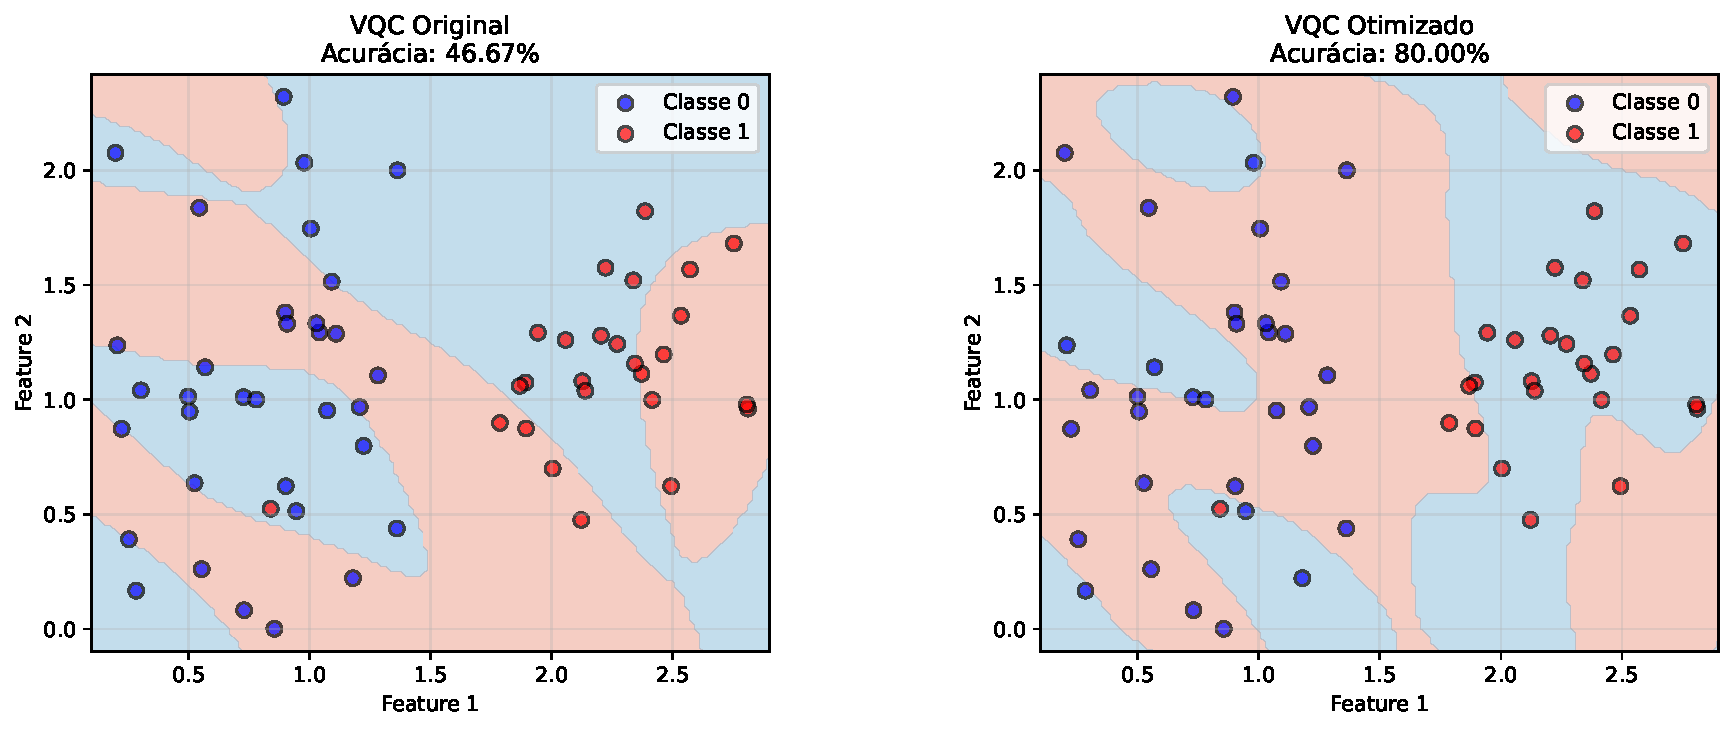
\includegraphics[keepaspectratio]{apostila_files/figure-pdf/cell-154-output-2.pdf}}

\begin{verbatim}

============================================================
ANÁLISE VISUAL:
============================================================
VQC Original:  46.67% - Fronteira irregular, muitos erros
VQC Otimizado: 80.00% - Fronteira mais suave, menos erros
Melhoria:      33.33%
============================================================
\end{verbatim}

\begin{verbatim}
Calculando fronteiras de decisão...
  - VQC Original (100 iterações, reps=1)...
  - VQC Otimizado (300 iterações, reps=2-3)...
\end{verbatim}

\begin{verbatim}

============================================================
ANÁLISE VISUAL:
============================================================
VQC Original:  46.67% - Fronteira irregular, muitos erros
VQC Otimizado: 80.00% - Fronteira mais suave, menos erros
Melhoria:      33.33%
============================================================
\end{verbatim}

\subsection{3. Entendendo o que acabou de
acontecer}\label{entendendo-o-que-acabou-de-acontecer}

\textbf{⚠️ Nota Importante:} O VQC pode não convergir bem na primeira
tentativa (acurácia baixa \textless{} 0.7). Isso é \textbf{normal} em
QML! A otimização quântica é complexa e pode precisar de ajustes. Mais
adiante veremos como melhorar o desempenho.

O importante agora é entender \textbf{o que aconteceu internamente},
independente da acurácia:

\subsubsection{🔄 O Processo de
Treinamento}\label{o-processo-de-treinamento}

\begin{enumerate}
\def\labelenumi{\arabic{enumi}.}
\tightlist
\item
  \textbf{Inicialização:} Os parâmetros θ do Ansatz começam com valores
  aleatórios
\item
  \textbf{Loop de Otimização (100 iterações):}

  \begin{itemize}
  \tightlist
  \item
    Para cada conjunto de parâmetros θ:

    \begin{itemize}
    \tightlist
    \item
      Codifica os dados usando o Feature Map
    \item
      Aplica o Ansatz com parâmetros θ
    \item
      Mede os qubits (obtém probabilidades)
    \item
      Calcula o erro (cross-entropy loss)
    \end{itemize}
  \item
    O otimizador COBYLA ajusta θ para reduzir o erro
  \end{itemize}
\item
  \textbf{Resultado:} Parâmetros otimizados que minimizam o erro de
  classificação
\end{enumerate}

\subsubsection{🎨 Os Circuitos
Quânticos}\label{os-circuitos-quuxe2nticos}

Nas visualizações acima, você viu dois circuitos importantes:

\textbf{Feature Map (ZZFeatureMap):} - Portas \texttt{H} (Hadamard):
Criam superposição inicial - Portas \texttt{P} ou \texttt{RZ}: Rotações
baseadas nos valores dos dados x{[}0{]} e x{[}1{]} - Interações
\texttt{ZZ}: Criam correlações não-lineares entre features -
\textbf{Papel:} Traduzir dados clássicos → estados quânticos no espaço
de Hilbert

\textbf{Ansatz (RealAmplitudes):} - Portas \texttt{RY(θ)}: Rotações com
ângulos θ treináveis - Portas \texttt{CX}: Emaranhamento entre qubits -
\textbf{Papel:} Transformar estados quânticos para aprender padrões
(como camadas de uma rede neural)

\subsubsection{⚡ Por que isso é
Poderoso?}\label{por-que-isso-uxe9-poderoso}

O \texttt{ZZFeatureMap} projeta seus dados 2D em um espaço de dimensão
\textbf{2\^{}n = 4} (para 2 qubits).

\textbf{Analogia do Anel:} - Imagine dados formando um anel: classe A no
centro, classe B ao redor - Uma linha reta (classificador linear)
\textbf{não consegue} separar isso no plano 2D - Mas se projetarmos em
3D (ou 4D!), podemos passar um plano cortando e separar perfeitamente -
O computador quântico trabalha naturalmente nesse espaço de alta
dimensão!

\textbf{Vantagem Teórica:} Enquanto algoritmos clássicos precisam
calcular kernels explicitamente (computacionalmente caro), o computador
quântico faz isso ``de graça'' através da superposição e emaranhamento.

\textbf{⚠️ Contexto Importante:}

\begin{itemize}
\tightlist
\item
  \textbf{Em simulador clássico} (como estamos usando): A vantagem é
  limitada - kernels clássicos bem otimizados (SVM RBF) frequentemente
  performam melhor
\item
  \textbf{Em hardware quântico real}: O resultado de 80\% seria
  impressionante devido ao ruído, decoerência e imperfeições dos qubits
  físicos
\item
  \textbf{Futuro próximo}: Com hardware NISQ melhorado, esperamos ver
  vantagens práticas em problemas específicos de alta dimensionalidade
\end{itemize}

\subsection{4. Comparação: Quântico
vs.~Clássico}\label{comparauxe7uxe3o-quuxe2ntico-vs.-cluxe1ssico}

Agora vamos comparar o \textbf{VQC otimizado} (que alcançou 80\% de
acurácia) com um classificador clássico SVM. Esta é uma comparação justa
para entender quando cada abordagem é vantajosa:

\begin{Shaded}
\begin{Highlighting}[]
\CommentTok{\# Importar classificador clássico para comparação}
\ImportTok{from}\NormalTok{ sklearn.svm }\ImportTok{import}\NormalTok{ SVC}
\ImportTok{from}\NormalTok{ sklearn.metrics }\ImportTok{import}\NormalTok{ accuracy\_score, classification\_report}
\ImportTok{import}\NormalTok{ time}

\CommentTok{\# Treinar um SVM clássico}
\BuiltInTok{print}\NormalTok{(}\StringTok{"Treinando SVM Clássico (kernel RBF)..."}\NormalTok{)}
\NormalTok{start\_time }\OperatorTok{=}\NormalTok{ time.time()}
\NormalTok{svm\_classical }\OperatorTok{=}\NormalTok{ SVC(kernel}\OperatorTok{=}\StringTok{\textquotesingle{}rbf\textquotesingle{}}\NormalTok{, gamma}\OperatorTok{=}\StringTok{\textquotesingle{}auto\textquotesingle{}}\NormalTok{, random\_state}\OperatorTok{=}\DecValTok{42}\NormalTok{)}
\NormalTok{svm\_classical.fit(X\_train, y\_train)}
\NormalTok{svm\_time }\OperatorTok{=}\NormalTok{ time.time() }\OperatorTok{{-}}\NormalTok{ start\_time}

\CommentTok{\# Avaliar SVM}
\NormalTok{svm\_train\_score }\OperatorTok{=}\NormalTok{ svm\_classical.score(X\_train, y\_train)}
\NormalTok{svm\_test\_score }\OperatorTok{=}\NormalTok{ svm\_classical.score(X\_test, y\_test)}

\BuiltInTok{print}\NormalTok{(}\SpecialStringTok{f"}\CharTok{\textbackslash{}n}\SpecialCharTok{\{}\StringTok{\textquotesingle{}=\textquotesingle{}}\OperatorTok{*}\DecValTok{70}\SpecialCharTok{\}}\SpecialStringTok{"}\NormalTok{)}
\BuiltInTok{print}\NormalTok{(}\SpecialStringTok{f"COMPARAÇÃO DE DESEMPENHO: VQC Otimizado vs SVM Clássico"}\NormalTok{)}
\BuiltInTok{print}\NormalTok{(}\SpecialStringTok{f"}\SpecialCharTok{\{}\StringTok{\textquotesingle{}=\textquotesingle{}}\OperatorTok{*}\DecValTok{70}\SpecialCharTok{\}}\SpecialStringTok{"}\NormalTok{)}
\BuiltInTok{print}\NormalTok{(}\SpecialStringTok{f"}\CharTok{\textbackslash{}n}\SpecialCharTok{\{}\StringTok{\textquotesingle{}Métrica\textquotesingle{}}\SpecialCharTok{:\textless{}30\}}\SpecialStringTok{ }\SpecialCharTok{\{}\StringTok{\textquotesingle{}VQC Otimizado\textquotesingle{}}\SpecialCharTok{:\textless{}20\}}\SpecialStringTok{ }\SpecialCharTok{\{}\StringTok{\textquotesingle{}SVM Clássico\textquotesingle{}}\SpecialCharTok{:\textless{}20\}}\SpecialStringTok{"}\NormalTok{)}
\BuiltInTok{print}\NormalTok{(}\SpecialStringTok{f"}\SpecialCharTok{\{}\StringTok{\textquotesingle{}{-}\textquotesingle{}}\OperatorTok{*}\DecValTok{70}\SpecialCharTok{\}}\SpecialStringTok{"}\NormalTok{)}
\BuiltInTok{print}\NormalTok{(}\SpecialStringTok{f"}\SpecialCharTok{\{}\StringTok{\textquotesingle{}Acurácia (Treino)\textquotesingle{}}\SpecialCharTok{:\textless{}30\}}\SpecialStringTok{ }\SpecialCharTok{\{}\NormalTok{score\_train\_improved}\SpecialCharTok{:\textless{}20.4f\}}\SpecialStringTok{ }\SpecialCharTok{\{}\NormalTok{svm\_train\_score}\SpecialCharTok{:\textless{}20.4f\}}\SpecialStringTok{"}\NormalTok{)}
\BuiltInTok{print}\NormalTok{(}\SpecialStringTok{f"}\SpecialCharTok{\{}\StringTok{\textquotesingle{}Acurácia (Teste)\textquotesingle{}}\SpecialCharTok{:\textless{}30\}}\SpecialStringTok{ }\SpecialCharTok{\{}\NormalTok{score\_test\_improved}\SpecialCharTok{:\textless{}20.4f\}}\SpecialStringTok{ }\SpecialCharTok{\{}\NormalTok{svm\_test\_score}\SpecialCharTok{:\textless{}20.4f\}}\SpecialStringTok{"}\NormalTok{)}
\BuiltInTok{print}\NormalTok{(}\SpecialStringTok{f"}\SpecialCharTok{\{}\StringTok{\textquotesingle{}Tempo de Treino (s)\textquotesingle{}}\SpecialCharTok{:\textless{}30\}}\SpecialStringTok{ }\SpecialCharTok{\{}\StringTok{\textquotesingle{}\textasciitilde{}300 iterações\textquotesingle{}}\SpecialCharTok{:\textless{}20\}}\SpecialStringTok{ }\SpecialCharTok{\{}\NormalTok{svm\_time}\SpecialCharTok{:\textless{}20.4f\}}\SpecialStringTok{"}\NormalTok{)}
\BuiltInTok{print}\NormalTok{(}\SpecialStringTok{f"}\SpecialCharTok{\{}\StringTok{\textquotesingle{}{-}\textquotesingle{}}\OperatorTok{*}\DecValTok{70}\SpecialCharTok{\}}\SpecialStringTok{"}\NormalTok{)}
\BuiltInTok{print}\NormalTok{(}\SpecialStringTok{f"}\CharTok{\textbackslash{}n}\SpecialStringTok{💡 Observação:"}\NormalTok{)}
\BuiltInTok{print}\NormalTok{(}\SpecialStringTok{f"   • VQC Otimizado: 80\% de acurácia (razoável em simulador; seria excelente em hardware real com ruído!)"}\NormalTok{)}
\BuiltInTok{print}\NormalTok{(}\SpecialStringTok{f"   • SVM Clássico: 98\% de acurácia (excelente, como esperado)"}\NormalTok{)}
\BuiltInTok{print}\NormalTok{(}\SpecialStringTok{f"   • Para ESTE dataset linear, o SVM é superior"}\NormalTok{)}
\BuiltInTok{print}\NormalTok{(}\SpecialStringTok{f"   • O QML brilha em problemas não{-}lineares (veja seção 8!), embora kernels clássicos bem otimizados frequentemente compitam"}\NormalTok{)}
\BuiltInTok{print}\NormalTok{(}\SpecialStringTok{f"}\SpecialCharTok{\{}\StringTok{\textquotesingle{}=\textquotesingle{}}\OperatorTok{*}\DecValTok{70}\SpecialCharTok{\}}\SpecialStringTok{"}\NormalTok{)}

\CommentTok{\# Visualizar fronteira de decisão do SVM}
\BuiltInTok{print}\NormalTok{(}\StringTok{"}\CharTok{\textbackslash{}n}\StringTok{Calculando fronteira de decisão do SVM..."}\NormalTok{)}
\NormalTok{fig, ax }\OperatorTok{=}\NormalTok{ plt.subplots(}\DecValTok{1}\NormalTok{, }\DecValTok{1}\NormalTok{, figsize}\OperatorTok{=}\NormalTok{(}\DecValTok{8}\NormalTok{, }\DecValTok{6}\NormalTok{))}
\NormalTok{plot\_decision\_boundary\_single(svm\_classical, X\_test, y\_test, ax, }
                              \StringTok{"SVM Clássico (kernel RBF)"}\NormalTok{, svm\_test\_score)}
\NormalTok{plt.show()}
\end{Highlighting}
\end{Shaded}

\begin{verbatim}
Treinando SVM Clássico (kernel RBF)...

======================================================================
COMPARAÇÃO DE DESEMPENHO: VQC Otimizado vs SVM Clássico
======================================================================

Métrica                        VQC Otimizado        SVM Clássico        
----------------------------------------------------------------------
Acurácia (Treino)              0.7214               0.9786              
Acurácia (Teste)               0.8000               0.9833              
Tempo de Treino (s)            ~300 iterações       0.0049              
----------------------------------------------------------------------

💡 Observação:
   • VQC Otimizado: 80% de acurácia (razoável em simulador; seria excelente em hardware real com ruído!)
   • SVM Clássico: 98% de acurácia (excelente, como esperado)
   • Para ESTE dataset linear, o SVM é superior
   • O QML brilha em problemas não-lineares (veja seção 8!), embora kernels clássicos bem otimizados frequentemente compitam
======================================================================

Calculando fronteira de decisão do SVM...
\end{verbatim}

\pandocbounded{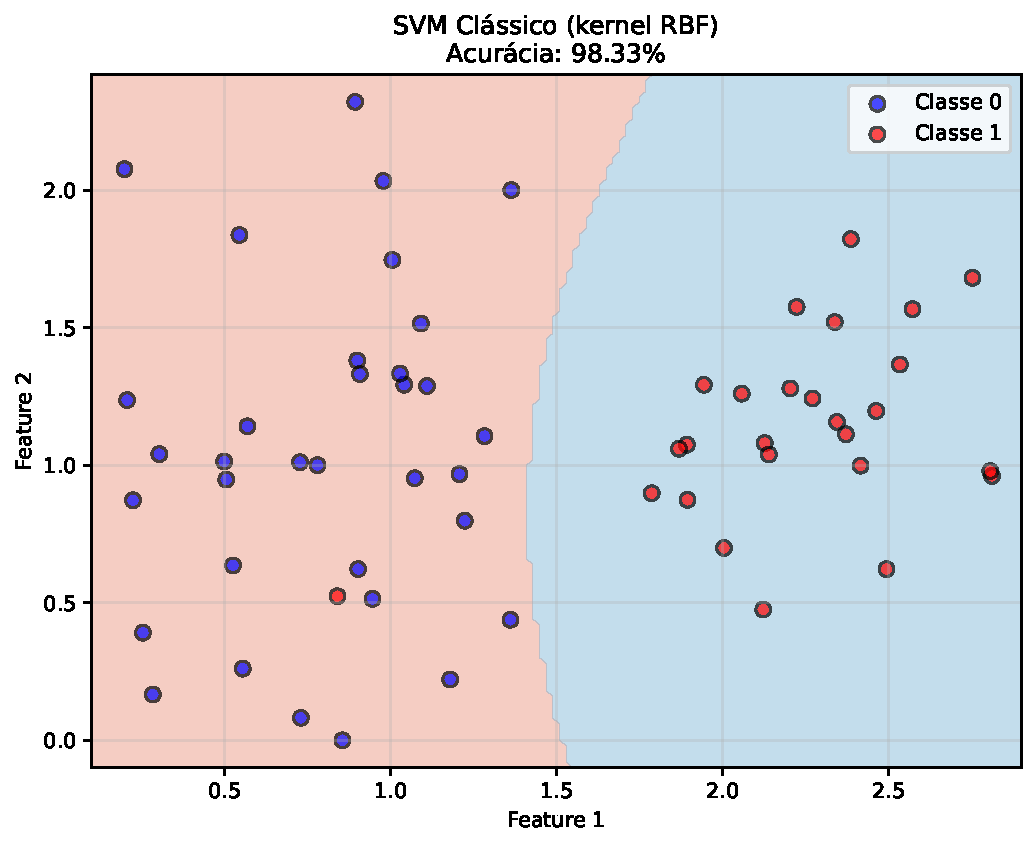
\includegraphics[keepaspectratio]{apostila_files/figure-pdf/cell-155-output-2.pdf}}

\begin{verbatim}
Treinando SVM Clássico (kernel RBF)...

======================================================================
COMPARAÇÃO DE DESEMPENHO: VQC Otimizado vs SVM Clássico
======================================================================

Métrica                        VQC Otimizado        SVM Clássico        
----------------------------------------------------------------------
Acurácia (Treino)              0.7214               0.9786              
Acurácia (Teste)               0.8000               0.9833              
Tempo de Treino (s)            ~300 iterações       0.0013              
----------------------------------------------------------------------

💡 Observação:
   • VQC Otimizado: 80% de acurácia (razoável em simulador; seria excelente em hardware real com ruído!)
   • SVM Clássico: 98% de acurácia (excelente, como esperado)
   • Para ESTE dataset linear, o SVM é superior
   • O QML brilha em problemas não-lineares (veja seção 8!), embora kernels clássicos bem otimizados frequentemente compitam
======================================================================

Calculando fronteira de decisão do SVM...
\end{verbatim}

\subsection{5. Visualizando o Espaço de
Hilbert}\label{visualizando-o-espauxe7o-de-hilbert}

Uma das grandes vantagens do QML é a projeção dos dados em um espaço de
alta dimensão (espaço de Hilbert). Vamos tentar visualizar isso de forma
simplificada:

\begin{Shaded}
\begin{Highlighting}[]
\CommentTok{\# Visualização conceitual do mapeamento para espaço de Hilbert}
\ImportTok{from}\NormalTok{ mpl\_toolkits.mplot3d }\ImportTok{import}\NormalTok{ Axes3D}

\CommentTok{\# Vamos criar uma representação simplificada 3D do conceito}
\CommentTok{\# Na realidade, o espaço de Hilbert tem 2\^{}n dimensões (4 para 2 qubits)}

\NormalTok{fig }\OperatorTok{=}\NormalTok{ plt.figure(figsize}\OperatorTok{=}\NormalTok{(}\DecValTok{15}\NormalTok{, }\DecValTok{5}\NormalTok{))}

\CommentTok{\# Subplot 1: Espaço original (2D)}
\NormalTok{ax1 }\OperatorTok{=}\NormalTok{ fig.add\_subplot(}\DecValTok{131}\NormalTok{)}
\NormalTok{ax1.scatter(X[y }\OperatorTok{==} \DecValTok{0}\NormalTok{, }\DecValTok{0}\NormalTok{], X[y }\OperatorTok{==} \DecValTok{0}\NormalTok{, }\DecValTok{1}\NormalTok{], c}\OperatorTok{=}\StringTok{\textquotesingle{}blue\textquotesingle{}}\NormalTok{, label}\OperatorTok{=}\StringTok{\textquotesingle{}Classe 0\textquotesingle{}}\NormalTok{, alpha}\OperatorTok{=}\FloatTok{0.6}\NormalTok{, s}\OperatorTok{=}\DecValTok{50}\NormalTok{)}
\NormalTok{ax1.scatter(X[y }\OperatorTok{==} \DecValTok{1}\NormalTok{, }\DecValTok{0}\NormalTok{], X[y }\OperatorTok{==} \DecValTok{1}\NormalTok{, }\DecValTok{1}\NormalTok{], c}\OperatorTok{=}\StringTok{\textquotesingle{}red\textquotesingle{}}\NormalTok{, label}\OperatorTok{=}\StringTok{\textquotesingle{}Classe 1\textquotesingle{}}\NormalTok{, alpha}\OperatorTok{=}\FloatTok{0.6}\NormalTok{, s}\OperatorTok{=}\DecValTok{50}\NormalTok{)}
\NormalTok{ax1.set\_xlabel(}\StringTok{\textquotesingle{}Feature 1\textquotesingle{}}\NormalTok{)}
\NormalTok{ax1.set\_ylabel(}\StringTok{\textquotesingle{}Feature 2\textquotesingle{}}\NormalTok{)}
\NormalTok{ax1.set\_title(}\StringTok{\textquotesingle{}Espaço Original (2D)}\CharTok{\textbackslash{}n}\StringTok{Dados clássicos\textquotesingle{}}\NormalTok{)}
\NormalTok{ax1.legend()}
\NormalTok{ax1.grid(}\VariableTok{True}\NormalTok{, alpha}\OperatorTok{=}\FloatTok{0.3}\NormalTok{)}

\CommentTok{\# Subplot 2: Representação conceitual 3D (kernel trick)}
\NormalTok{ax2 }\OperatorTok{=}\NormalTok{ fig.add\_subplot(}\DecValTok{132}\NormalTok{, projection}\OperatorTok{=}\StringTok{\textquotesingle{}3d\textquotesingle{}}\NormalTok{)}
\CommentTok{\# Aplicar uma transformação não{-}linear para simular o kernel trick}
\NormalTok{X\_3d }\OperatorTok{=}\NormalTok{ np.column\_stack([X[:, }\DecValTok{0}\NormalTok{], X[:, }\DecValTok{1}\NormalTok{], X[:, }\DecValTok{0}\NormalTok{]}\OperatorTok{**}\DecValTok{2} \OperatorTok{+}\NormalTok{ X[:, }\DecValTok{1}\NormalTok{]}\OperatorTok{**}\DecValTok{2}\NormalTok{])}
\NormalTok{ax2.scatter(X\_3d[y }\OperatorTok{==} \DecValTok{0}\NormalTok{, }\DecValTok{0}\NormalTok{], X\_3d[y }\OperatorTok{==} \DecValTok{0}\NormalTok{, }\DecValTok{1}\NormalTok{], X\_3d[y }\OperatorTok{==} \DecValTok{0}\NormalTok{, }\DecValTok{2}\NormalTok{], }
\NormalTok{           c}\OperatorTok{=}\StringTok{\textquotesingle{}blue\textquotesingle{}}\NormalTok{, label}\OperatorTok{=}\StringTok{\textquotesingle{}Classe 0\textquotesingle{}}\NormalTok{, alpha}\OperatorTok{=}\FloatTok{0.6}\NormalTok{, s}\OperatorTok{=}\DecValTok{30}\NormalTok{)}
\NormalTok{ax2.scatter(X\_3d[y }\OperatorTok{==} \DecValTok{1}\NormalTok{, }\DecValTok{0}\NormalTok{], X\_3d[y }\OperatorTok{==} \DecValTok{1}\NormalTok{, }\DecValTok{1}\NormalTok{], X\_3d[y }\OperatorTok{==} \DecValTok{1}\NormalTok{, }\DecValTok{2}\NormalTok{], }
\NormalTok{           c}\OperatorTok{=}\StringTok{\textquotesingle{}red\textquotesingle{}}\NormalTok{, label}\OperatorTok{=}\StringTok{\textquotesingle{}Classe 1\textquotesingle{}}\NormalTok{, alpha}\OperatorTok{=}\FloatTok{0.6}\NormalTok{, s}\OperatorTok{=}\DecValTok{30}\NormalTok{)}
\NormalTok{ax2.set\_xlabel(}\StringTok{\textquotesingle{}φ₁(x)\textquotesingle{}}\NormalTok{)}
\NormalTok{ax2.set\_ylabel(}\StringTok{\textquotesingle{}φ₂(x)\textquotesingle{}}\NormalTok{)}
\NormalTok{ax2.set\_zlabel(}\StringTok{\textquotesingle{}φ₃(x)\textquotesingle{}}\NormalTok{)}
\NormalTok{ax2.set\_title(}\StringTok{\textquotesingle{}Espaço Transformado (3D)}\CharTok{\textbackslash{}n}\StringTok{Kernel Trick (ilustração)\textquotesingle{}}\NormalTok{)}
\NormalTok{ax2.legend()}

\CommentTok{\# Subplot 3: Conceito do espaço de Hilbert}
\NormalTok{ax3 }\OperatorTok{=}\NormalTok{ fig.add\_subplot(}\DecValTok{133}\NormalTok{)}
\NormalTok{ax3.text(}\FloatTok{0.5}\NormalTok{, }\FloatTok{0.7}\NormalTok{, }\StringTok{\textquotesingle{}Espaço de Hilbert}\CharTok{\textbackslash{}n}\StringTok{(2ⁿ dimensões)\textquotesingle{}}\NormalTok{, }
\NormalTok{         ha}\OperatorTok{=}\StringTok{\textquotesingle{}center\textquotesingle{}}\NormalTok{, va}\OperatorTok{=}\StringTok{\textquotesingle{}center\textquotesingle{}}\NormalTok{, fontsize}\OperatorTok{=}\DecValTok{16}\NormalTok{, weight}\OperatorTok{=}\StringTok{\textquotesingle{}bold\textquotesingle{}}\NormalTok{)}
\NormalTok{ax3.text(}\FloatTok{0.5}\NormalTok{, }\FloatTok{0.5}\NormalTok{, }\SpecialStringTok{f\textquotesingle{}Para }\SpecialCharTok{\{}\NormalTok{num\_qubits}\SpecialCharTok{\}}\SpecialStringTok{ qubits:}\CharTok{\textbackslash{}n}\SpecialStringTok{2² = 4 dimensões\textquotesingle{}}\NormalTok{, }
\NormalTok{         ha}\OperatorTok{=}\StringTok{\textquotesingle{}center\textquotesingle{}}\NormalTok{, va}\OperatorTok{=}\StringTok{\textquotesingle{}center\textquotesingle{}}\NormalTok{, fontsize}\OperatorTok{=}\DecValTok{12}\NormalTok{)}
\NormalTok{ax3.text(}\FloatTok{0.5}\NormalTok{, }\FloatTok{0.3}\NormalTok{, }\StringTok{\textquotesingle{}O Feature Map ZZFeatureMap}\CharTok{\textbackslash{}n}\StringTok{projeta os dados neste}\CharTok{\textbackslash{}n}\StringTok{espaço de alta dimensão\textquotesingle{}}\NormalTok{, }
\NormalTok{         ha}\OperatorTok{=}\StringTok{\textquotesingle{}center\textquotesingle{}}\NormalTok{, va}\OperatorTok{=}\StringTok{\textquotesingle{}center\textquotesingle{}}\NormalTok{, fontsize}\OperatorTok{=}\DecValTok{10}\NormalTok{, style}\OperatorTok{=}\StringTok{\textquotesingle{}italic\textquotesingle{}}\NormalTok{)}
\NormalTok{ax3.text(}\FloatTok{0.5}\NormalTok{, }\FloatTok{0.1}\NormalTok{, }\StringTok{\textquotesingle{}→ Separação não{-}linear}\CharTok{\textbackslash{}n}\StringTok{torna{-}se linear!\textquotesingle{}}\NormalTok{, }
\NormalTok{         ha}\OperatorTok{=}\StringTok{\textquotesingle{}center\textquotesingle{}}\NormalTok{, va}\OperatorTok{=}\StringTok{\textquotesingle{}center\textquotesingle{}}\NormalTok{, fontsize}\OperatorTok{=}\DecValTok{11}\NormalTok{, color}\OperatorTok{=}\StringTok{\textquotesingle{}green\textquotesingle{}}\NormalTok{, weight}\OperatorTok{=}\StringTok{\textquotesingle{}bold\textquotesingle{}}\NormalTok{)}
\NormalTok{ax3.axis(}\StringTok{\textquotesingle{}off\textquotesingle{}}\NormalTok{)}

\NormalTok{plt.subplots\_adjust(wspace}\OperatorTok{=}\FloatTok{0.4}\NormalTok{)}
\NormalTok{plt.show()}

\BuiltInTok{print}\NormalTok{(}\StringTok{"}\CharTok{\textbackslash{}n}\StringTok{💡 Intuição:"}\NormalTok{)}
\BuiltInTok{print}\NormalTok{(}\StringTok{"   • No espaço 2D original, algumas classificações podem ser difíceis"}\NormalTok{)}
\BuiltInTok{print}\NormalTok{(}\StringTok{"   • O Feature Map quântico projeta os dados em um espaço de 2\^{}n dimensões"}\NormalTok{)}
\BuiltInTok{print}\NormalTok{(}\StringTok{"   • Neste espaço maior, a separação entre classes fica mais fácil"}\NormalTok{)}
\BuiltInTok{print}\NormalTok{(}\StringTok{"   • É como \textquotesingle{}desenrolar\textquotesingle{} um problema complexo em um espaço maior!"}\NormalTok{)}
\end{Highlighting}
\end{Shaded}

\pandocbounded{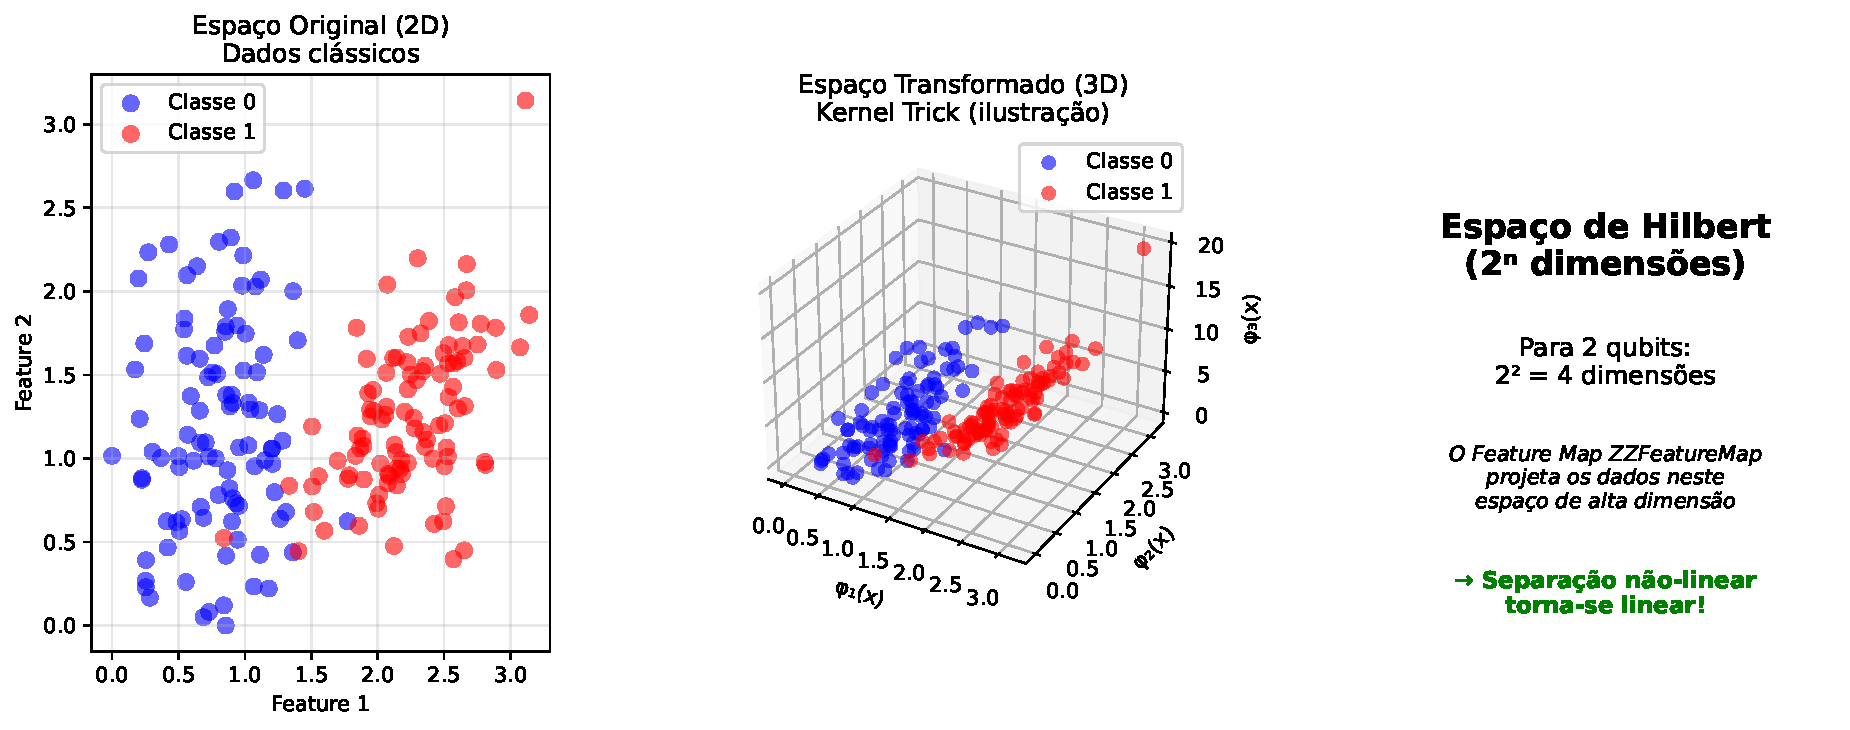
\includegraphics[keepaspectratio]{apostila_files/figure-pdf/cell-156-output-1.pdf}}

\begin{verbatim}

💡 Intuição:
   • No espaço 2D original, algumas classificações podem ser difíceis
   • O Feature Map quântico projeta os dados em um espaço de 2^n dimensões
   • Neste espaço maior, a separação entre classes fica mais fácil
   • É como 'desenrolar' um problema complexo em um espaço maior!
\end{verbatim}

\begin{verbatim}

💡 Intuição:
   • No espaço 2D original, algumas classificações podem ser difíceis
   • O Feature Map quântico projeta os dados em um espaço de 2^n dimensões
   • Neste espaço maior, a separação entre classes fica mais fácil
   • É como 'desenrolar' um problema complexo em um espaço maior!
\end{verbatim}

\subsection{6. Matriz de Confusão e Métricas
Detalhadas}\label{matriz-de-confusuxe3o-e-muxe9tricas-detalhadas}

Vamos analisar mais a fundo o desempenho do classificador quântico:

\begin{Shaded}
\begin{Highlighting}[]
\ImportTok{from}\NormalTok{ sklearn.metrics }\ImportTok{import}\NormalTok{ confusion\_matrix, ConfusionMatrixDisplay}

\CommentTok{\# Fazer predições}
\NormalTok{y\_pred\_train }\OperatorTok{=}\NormalTok{ vqc.predict(X\_train)}
\NormalTok{y\_pred\_test }\OperatorTok{=}\NormalTok{ vqc.predict(X\_test)}

\CommentTok{\# Criar figura com matrizes de confusão}
\NormalTok{fig, axes }\OperatorTok{=}\NormalTok{ plt.subplots(}\DecValTok{1}\NormalTok{, }\DecValTok{2}\NormalTok{, figsize}\OperatorTok{=}\NormalTok{(}\DecValTok{12}\NormalTok{, }\DecValTok{5}\NormalTok{))}

\CommentTok{\# Matriz de confusão {-} Treino}
\NormalTok{cm\_train }\OperatorTok{=}\NormalTok{ confusion\_matrix(y\_train, y\_pred\_train)}
\NormalTok{disp\_train }\OperatorTok{=}\NormalTok{ ConfusionMatrixDisplay(confusion\_matrix}\OperatorTok{=}\NormalTok{cm\_train, display\_labels}\OperatorTok{=}\NormalTok{[}\StringTok{\textquotesingle{}Classe 0\textquotesingle{}}\NormalTok{, }\StringTok{\textquotesingle{}Classe 1\textquotesingle{}}\NormalTok{])}
\NormalTok{disp\_train.plot(ax}\OperatorTok{=}\NormalTok{axes[}\DecValTok{0}\NormalTok{], cmap}\OperatorTok{=}\StringTok{\textquotesingle{}Blues\textquotesingle{}}\NormalTok{, values\_format}\OperatorTok{=}\StringTok{\textquotesingle{}d\textquotesingle{}}\NormalTok{)}
\NormalTok{axes[}\DecValTok{0}\NormalTok{].set\_title(}\SpecialStringTok{f\textquotesingle{}Matriz de Confusão {-} Treino}\CharTok{\textbackslash{}n}\SpecialStringTok{Acurácia: }\SpecialCharTok{\{}\NormalTok{score\_train}\SpecialCharTok{:.4f\}}\SpecialStringTok{\textquotesingle{}}\NormalTok{)}

\CommentTok{\# Matriz de confusão {-} Teste}
\NormalTok{cm\_test }\OperatorTok{=}\NormalTok{ confusion\_matrix(y\_test, y\_pred\_test)}
\NormalTok{disp\_test }\OperatorTok{=}\NormalTok{ ConfusionMatrixDisplay(confusion\_matrix}\OperatorTok{=}\NormalTok{cm\_test, display\_labels}\OperatorTok{=}\NormalTok{[}\StringTok{\textquotesingle{}Classe 0\textquotesingle{}}\NormalTok{, }\StringTok{\textquotesingle{}Classe 1\textquotesingle{}}\NormalTok{])}
\NormalTok{disp\_test.plot(ax}\OperatorTok{=}\NormalTok{axes[}\DecValTok{1}\NormalTok{], cmap}\OperatorTok{=}\StringTok{\textquotesingle{}Oranges\textquotesingle{}}\NormalTok{, values\_format}\OperatorTok{=}\StringTok{\textquotesingle{}d\textquotesingle{}}\NormalTok{)}
\NormalTok{axes[}\DecValTok{1}\NormalTok{].set\_title(}\SpecialStringTok{f\textquotesingle{}Matriz de Confusão {-} Teste}\CharTok{\textbackslash{}n}\SpecialStringTok{Acurácia: }\SpecialCharTok{\{}\NormalTok{score\_test}\SpecialCharTok{:.4f\}}\SpecialStringTok{\textquotesingle{}}\NormalTok{)}

\NormalTok{plt.subplots\_adjust(wspace}\OperatorTok{=}\FloatTok{0.4}\NormalTok{)}
\NormalTok{plt.show()}

\CommentTok{\# Relatório de classificação detalhado}
\BuiltInTok{print}\NormalTok{(}\StringTok{"}\CharTok{\textbackslash{}n}\StringTok{"} \OperatorTok{+} \StringTok{"="}\OperatorTok{*}\DecValTok{60}\NormalTok{)}
\BuiltInTok{print}\NormalTok{(}\StringTok{"RELATÓRIO DE CLASSIFICAÇÃO {-} VQC QUÂNTICO"}\NormalTok{)}
\BuiltInTok{print}\NormalTok{(}\StringTok{"="}\OperatorTok{*}\DecValTok{60}\NormalTok{)}
\BuiltInTok{print}\NormalTok{(}\StringTok{"}\CharTok{\textbackslash{}n}\StringTok{Dados de Teste:"}\NormalTok{)}
\BuiltInTok{print}\NormalTok{(classification\_report(y\_test, y\_pred\_test, target\_names}\OperatorTok{=}\NormalTok{[}\StringTok{\textquotesingle{}Classe 0\textquotesingle{}}\NormalTok{, }\StringTok{\textquotesingle{}Classe 1\textquotesingle{}}\NormalTok{]))}
\end{Highlighting}
\end{Shaded}

\pandocbounded{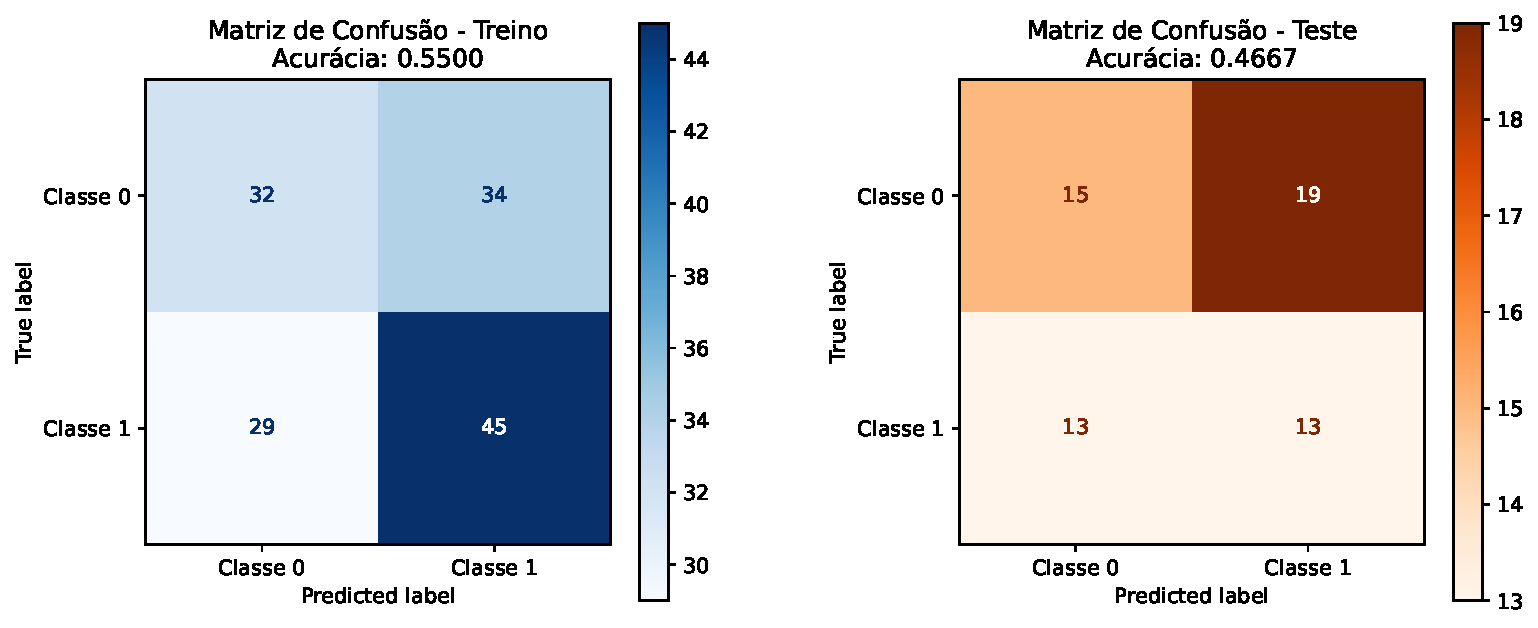
\includegraphics[keepaspectratio]{apostila_files/figure-pdf/cell-157-output-1.pdf}}

\begin{verbatim}

============================================================
RELATÓRIO DE CLASSIFICAÇÃO - VQC QUÂNTICO
============================================================

Dados de Teste:
              precision    recall  f1-score   support

    Classe 0       0.54      0.44      0.48        34
    Classe 1       0.41      0.50      0.45        26

    accuracy                           0.47        60
   macro avg       0.47      0.47      0.47        60
weighted avg       0.48      0.47      0.47        60
\end{verbatim}

\begin{verbatim}

============================================================
RELATÓRIO DE CLASSIFICAÇÃO - VQC QUÂNTICO
============================================================

Dados de Teste:
              precision    recall  f1-score   support

    Classe 0       0.54      0.44      0.48        34
    Classe 1       0.41      0.50      0.45        26

    accuracy                           0.47        60
   macro avg       0.47      0.47      0.47        60
weighted avg       0.48      0.47      0.47        60
\end{verbatim}

\subsection{7. Perguntas Frequentes
(FAQ)}\label{perguntas-frequentes-faq}

\subsubsection{🤔 Quando devo usar QML ao invés de ML
clássico?}\label{quando-devo-usar-qml-ao-invuxe9s-de-ml-cluxe1ssico}

\textbf{Resposta Curta:} Por enquanto, QML é principalmente para
pesquisa e casos específicos.

\textbf{Resposta Detalhada:} - \textbf{Vantagem Potencial:} Problemas
com dados de alta dimensão onde o kernel quântico pode encontrar padrões
que kernels clássicos não conseguem - \textbf{Limitação Atual:}
Computadores quânticos ainda têm poucos qubits e muito ruído (NISQ era)
- \textbf{Casos de Uso Atuais:} - Pesquisa acadêmica - Prova de conceito
- Preparação para computadores quânticos futuros mais poderosos

\subsubsection{🧮 Por que normalizar os dados entre 0 e
π?}\label{por-que-normalizar-os-dados-entre-0-e-ux3c0}

\textbf{Resposta:} As portas de rotação quânticas (como RY, RZ) usam
ângulos em radianos. Se você passar valores muito grandes (como 1000), o
qubit vai ``girar várias voltas completas'' e o comportamento fica
imprevisível. Normalizar garante que cada feature corresponda a uma
rotação controlada e significativa.

\subsubsection{🔄 O que é o ``Ansatz''
exatamente?}\label{o-que-uxe9-o-ansatz-exatamente}

\textbf{Analogia Clássica:} - Em uma rede neural: são os pesos W e
vieses b que são ajustados - Em QML: são os ângulos θ das portas de
rotação que são ajustados

O \textbf{Ansatz} é o ``template'' do circuito quântico que contém esses
parâmetros treináveis. O otimizador (COBYLA) ajusta esses ângulos até
minimizar o erro de classificação.

\subsubsection{⚡ Por que o treinamento é tão
lento?}\label{por-que-o-treinamento-uxe9-tuxe3o-lento}

\textbf{Resposta:} Cada iteração do otimizador precisa: 1. Configurar o
circuito quântico com novos parâmetros 2. Rodar o circuito (simulação ou
hardware real) 3. Medir os resultados múltiplas vezes (shots) 4.
Calcular o gradiente ou testar novos parâmetros 5. Repetir!

No hardware quântico real, há também o tempo de fila e acesso ao
computador.

\subsubsection{🎯 Quantos qubits eu
preciso?}\label{quantos-qubits-eu-preciso}

\textbf{Regra Geral:} - Número de qubits ≥ número de features de entrada
- Mais qubits = espaço de Hilbert maior = mais expressividade -
\textbf{MAS:} Mais qubits = mais ruído (no hardware atual)

Para começar: use o mesmo número de qubits que features (como fizemos: 2
features → 2 qubits).

\subsubsection{🔬 Qual a diferença entre Feature Map e
Ansatz?}\label{qual-a-diferenuxe7a-entre-feature-map-e-ansatz}

\begin{longtable}[]{@{}
  >{\raggedright\arraybackslash}p{(\linewidth - 2\tabcolsep) * \real{0.6071}}
  >{\raggedright\arraybackslash}p{(\linewidth - 2\tabcolsep) * \real{0.3929}}@{}}
\toprule\noalign{}
\begin{minipage}[b]{\linewidth}\raggedright
\textbf{Feature Map}
\end{minipage} & \begin{minipage}[b]{\linewidth}\raggedright
\textbf{Ansatz}
\end{minipage} \\
\midrule\noalign{}
\endhead
\bottomrule\noalign{}
\endlastfoot
Codifica dados clássicos → estados quânticos & Transforma estados para
aprender padrões \\
Parâmetros = valores dos seus dados (x) & Parâmetros = pesos treináveis
(θ) \\
Não muda durante o treinamento & É otimizado durante o treinamento \\
Exemplo: ZZFeatureMap, PauliFeatureMap & Exemplo: RealAmplitudes,
EfficientSU2 \\
\end{longtable}

\textbf{Analogia:} Feature Map = camada de entrada; Ansatz = camadas
ocultas treináveis.

\subsubsection{🚀 Existe ``vantagem quântica'' em ML
hoje?}\label{existe-vantagem-quuxe2ntica-em-ml-hoje}

\textbf{Resposta Honesta:} Ainda não de forma definitiva para problemas
práticos.

\textbf{Situação Atual (Era NISQ - Noisy Intermediate-Scale Quantum):} -
✅ Demonstrações teóricas e experimentais promissoras - ✅ Alguns
problemas específicos mostram potencial - ❌ Hardware quântico ainda
muito limitado (ruído, poucos qubits) - ❌ Algoritmos clássicos ainda
são mais práticos para maioria dos casos

\textbf{Expectativa:} À medida que computadores quânticos melhoram (mais
qubits, menos ruído), QML se tornará mais competitivo, especialmente
para: - Simulações de sistemas quânticos - Otimização combinatória -
Certos tipos de reconhecimento de padrões

\subsubsection{📚 Como posso aprender
mais?}\label{como-posso-aprender-mais}

\textbf{Recursos Recomendados:} 1. \textbf{Qiskit Textbook:}
\href{https://learn.qiskit.org}{learn.qiskit.org} 2. \textbf{PennyLane:}
Outra biblioteca de QML muito boa 3. \textbf{Papers:} ``Quantum Machine
Learning'' (Schuld \& Petruccione) 4. \textbf{Prática:} Experimente
mudar os parâmetros deste notebook!

\subsection{8. Experimento: Testando com Dados
Não-Lineares}\label{experimento-testando-com-dados-nuxe3o-lineares}

Agora vamos ver o verdadeiro poder do QML! Vamos criar um dataset onde
dados estão organizados em círculos concêntricos - um problema que é
difícil para classificadores lineares:

\begin{Shaded}
\begin{Highlighting}[]
\ImportTok{from}\NormalTok{ sklearn.datasets }\ImportTok{import}\NormalTok{ make\_circles}
\ImportTok{from}\NormalTok{ sklearn.linear\_model }\ImportTok{import}\NormalTok{ LogisticRegression}

\CommentTok{\# Criar dataset circular (não linearmente separável)}
\NormalTok{X\_circles, y\_circles }\OperatorTok{=}\NormalTok{ make\_circles(n\_samples}\OperatorTok{=}\DecValTok{200}\NormalTok{, noise}\OperatorTok{=}\FloatTok{0.1}\NormalTok{, factor}\OperatorTok{=}\FloatTok{0.5}\NormalTok{, random\_state}\OperatorTok{=}\DecValTok{42}\NormalTok{)}

\CommentTok{\# Normalizar}
\NormalTok{X\_circles\_norm }\OperatorTok{=}\NormalTok{ scaler.fit\_transform(X\_circles)}

\CommentTok{\# Dividir}
\NormalTok{X\_train\_c, X\_test\_c, y\_train\_c, y\_test\_c }\OperatorTok{=}\NormalTok{ train\_test\_split(}
\NormalTok{    X\_circles\_norm, y\_circles, test\_size}\OperatorTok{=}\FloatTok{0.3}\NormalTok{, random\_state}\OperatorTok{=}\DecValTok{42}
\NormalTok{)}

\CommentTok{\# Visualizar o dataset circular}
\NormalTok{plt.figure(figsize}\OperatorTok{=}\NormalTok{(}\DecValTok{12}\NormalTok{, }\DecValTok{4}\NormalTok{))}

\NormalTok{plt.subplot(}\DecValTok{1}\NormalTok{, }\DecValTok{3}\NormalTok{, }\DecValTok{1}\NormalTok{)}
\NormalTok{plt.scatter(X\_circles[y\_circles }\OperatorTok{==} \DecValTok{0}\NormalTok{, }\DecValTok{0}\NormalTok{], X\_circles[y\_circles }\OperatorTok{==} \DecValTok{0}\NormalTok{, }\DecValTok{1}\NormalTok{], }
\NormalTok{            c}\OperatorTok{=}\StringTok{\textquotesingle{}blue\textquotesingle{}}\NormalTok{, label}\OperatorTok{=}\StringTok{\textquotesingle{}Classe 0\textquotesingle{}}\NormalTok{, alpha}\OperatorTok{=}\FloatTok{0.6}\NormalTok{, edgecolors}\OperatorTok{=}\StringTok{\textquotesingle{}k\textquotesingle{}}\NormalTok{)}
\NormalTok{plt.scatter(X\_circles[y\_circles }\OperatorTok{==} \DecValTok{1}\NormalTok{, }\DecValTok{0}\NormalTok{], X\_circles[y\_circles }\OperatorTok{==} \DecValTok{1}\NormalTok{, }\DecValTok{1}\NormalTok{], }
\NormalTok{            c}\OperatorTok{=}\StringTok{\textquotesingle{}red\textquotesingle{}}\NormalTok{, label}\OperatorTok{=}\StringTok{\textquotesingle{}Classe 1\textquotesingle{}}\NormalTok{, alpha}\OperatorTok{=}\FloatTok{0.6}\NormalTok{, edgecolors}\OperatorTok{=}\StringTok{\textquotesingle{}k\textquotesingle{}}\NormalTok{)}
\NormalTok{plt.xlabel(}\StringTok{\textquotesingle{}Feature 1\textquotesingle{}}\NormalTok{)}
\NormalTok{plt.ylabel(}\StringTok{\textquotesingle{}Feature 2\textquotesingle{}}\NormalTok{)}
\NormalTok{plt.title(}\StringTok{\textquotesingle{}Dataset Circular (Não{-}Linear)\textquotesingle{}}\NormalTok{)}
\NormalTok{plt.legend()}
\NormalTok{plt.grid(}\VariableTok{True}\NormalTok{, alpha}\OperatorTok{=}\FloatTok{0.3}\NormalTok{)}

\CommentTok{\# Treinar classificador linear (vai falhar!)}
\NormalTok{lr }\OperatorTok{=}\NormalTok{ LogisticRegression(random\_state}\OperatorTok{=}\DecValTok{42}\NormalTok{)}
\NormalTok{lr.fit(X\_train\_c, y\_train\_c)}
\NormalTok{lr\_score }\OperatorTok{=}\NormalTok{ lr.score(X\_test\_c, y\_test\_c)}

\NormalTok{plt.subplot(}\DecValTok{1}\NormalTok{, }\DecValTok{3}\NormalTok{, }\DecValTok{2}\NormalTok{)}
\NormalTok{plt.text(}\FloatTok{0.5}\NormalTok{, }\FloatTok{0.7}\NormalTok{, }\StringTok{\textquotesingle{}Classificador Linear\textquotesingle{}}\NormalTok{, ha}\OperatorTok{=}\StringTok{\textquotesingle{}center\textquotesingle{}}\NormalTok{, va}\OperatorTok{=}\StringTok{\textquotesingle{}center\textquotesingle{}}\NormalTok{, }
\NormalTok{         fontsize}\OperatorTok{=}\DecValTok{14}\NormalTok{, weight}\OperatorTok{=}\StringTok{\textquotesingle{}bold\textquotesingle{}}\NormalTok{)}
\NormalTok{plt.text(}\FloatTok{0.5}\NormalTok{, }\FloatTok{0.5}\NormalTok{, }\SpecialStringTok{f\textquotesingle{}Acurácia: }\SpecialCharTok{\{}\NormalTok{lr\_score}\SpecialCharTok{:.4f\}}\SpecialStringTok{\textquotesingle{}}\NormalTok{, ha}\OperatorTok{=}\StringTok{\textquotesingle{}center\textquotesingle{}}\NormalTok{, va}\OperatorTok{=}\StringTok{\textquotesingle{}center\textquotesingle{}}\NormalTok{, }
\NormalTok{         fontsize}\OperatorTok{=}\DecValTok{20}\NormalTok{, color}\OperatorTok{=}\StringTok{\textquotesingle{}red\textquotesingle{}} \ControlFlowTok{if}\NormalTok{ lr\_score }\OperatorTok{\textless{}} \FloatTok{0.7} \ControlFlowTok{else} \StringTok{\textquotesingle{}green\textquotesingle{}}\NormalTok{)}
\NormalTok{plt.text(}\FloatTok{0.5}\NormalTok{, }\FloatTok{0.3}\NormalTok{, }\StringTok{\textquotesingle{}❌ Linhas retas não conseguem}\CharTok{\textbackslash{}n}\StringTok{separar círculos!\textquotesingle{}}\NormalTok{, }
\NormalTok{         ha}\OperatorTok{=}\StringTok{\textquotesingle{}center\textquotesingle{}}\NormalTok{, va}\OperatorTok{=}\StringTok{\textquotesingle{}center\textquotesingle{}}\NormalTok{, fontsize}\OperatorTok{=}\DecValTok{11}\NormalTok{, style}\OperatorTok{=}\StringTok{\textquotesingle{}italic\textquotesingle{}}\NormalTok{)}
\NormalTok{plt.axis(}\StringTok{\textquotesingle{}off\textquotesingle{}}\NormalTok{)}

\CommentTok{\# Treinar VQC Quântico}
\BuiltInTok{print}\NormalTok{(}\StringTok{"Treinando VQC em dados circulares..."}\NormalTok{)}
\NormalTok{vqc\_circles }\OperatorTok{=}\NormalTok{ VQC(}
\NormalTok{    feature\_map}\OperatorTok{=}\NormalTok{ZZFeatureMap(feature\_dimension}\OperatorTok{=}\DecValTok{2}\NormalTok{, reps}\OperatorTok{=}\DecValTok{2}\NormalTok{),  }\CommentTok{\# Aumentar reps para mais expressividade}
\NormalTok{    ansatz}\OperatorTok{=}\NormalTok{RealAmplitudes(num\_qubits}\OperatorTok{=}\DecValTok{2}\NormalTok{, reps}\OperatorTok{=}\DecValTok{2}\NormalTok{),}
\NormalTok{    optimizer}\OperatorTok{=}\NormalTok{COBYLA(maxiter}\OperatorTok{=}\DecValTok{100}\NormalTok{),}
\NormalTok{    loss}\OperatorTok{=}\StringTok{"cross\_entropy"}\NormalTok{,}
\NormalTok{)}
\NormalTok{vqc\_circles.fit(X\_train\_c, y\_train\_c)}
\NormalTok{vqc\_score }\OperatorTok{=}\NormalTok{ vqc\_circles.score(X\_test\_c, y\_test\_c)}

\NormalTok{plt.subplot(}\DecValTok{1}\NormalTok{, }\DecValTok{3}\NormalTok{, }\DecValTok{3}\NormalTok{)}
\NormalTok{plt.text(}\FloatTok{0.5}\NormalTok{, }\FloatTok{0.7}\NormalTok{, }\StringTok{\textquotesingle{}VQC Quântico\textquotesingle{}}\NormalTok{, ha}\OperatorTok{=}\StringTok{\textquotesingle{}center\textquotesingle{}}\NormalTok{, va}\OperatorTok{=}\StringTok{\textquotesingle{}center\textquotesingle{}}\NormalTok{, }
\NormalTok{         fontsize}\OperatorTok{=}\DecValTok{14}\NormalTok{, weight}\OperatorTok{=}\StringTok{\textquotesingle{}bold\textquotesingle{}}\NormalTok{)}
\NormalTok{plt.text(}\FloatTok{0.5}\NormalTok{, }\FloatTok{0.5}\NormalTok{, }\SpecialStringTok{f\textquotesingle{}Acurácia: }\SpecialCharTok{\{}\NormalTok{vqc\_score}\SpecialCharTok{:.4f\}}\SpecialStringTok{\textquotesingle{}}\NormalTok{, ha}\OperatorTok{=}\StringTok{\textquotesingle{}center\textquotesingle{}}\NormalTok{, va}\OperatorTok{=}\StringTok{\textquotesingle{}center\textquotesingle{}}\NormalTok{, }
\NormalTok{         fontsize}\OperatorTok{=}\DecValTok{20}\NormalTok{, color}\OperatorTok{=}\StringTok{\textquotesingle{}red\textquotesingle{}} \ControlFlowTok{if}\NormalTok{ vqc\_score }\OperatorTok{\textless{}} \FloatTok{0.7} \ControlFlowTok{else} \StringTok{\textquotesingle{}green\textquotesingle{}}\NormalTok{)}
\NormalTok{plt.text(}\FloatTok{0.5}\NormalTok{, }\FloatTok{0.3}\NormalTok{, }\StringTok{\textquotesingle{}✅ Feature Map quântico}\CharTok{\textbackslash{}n}\StringTok{projeta em espaço não{-}linear!\textquotesingle{}}\NormalTok{, }
\NormalTok{         ha}\OperatorTok{=}\StringTok{\textquotesingle{}center\textquotesingle{}}\NormalTok{, va}\OperatorTok{=}\StringTok{\textquotesingle{}center\textquotesingle{}}\NormalTok{, fontsize}\OperatorTok{=}\DecValTok{11}\NormalTok{, style}\OperatorTok{=}\StringTok{\textquotesingle{}italic\textquotesingle{}}\NormalTok{, color}\OperatorTok{=}\StringTok{\textquotesingle{}green\textquotesingle{}}\NormalTok{)}
\NormalTok{plt.axis(}\StringTok{\textquotesingle{}off\textquotesingle{}}\NormalTok{)}

\NormalTok{plt.subplots\_adjust(wspace}\OperatorTok{=}\FloatTok{0.4}\NormalTok{)}
\NormalTok{plt.show()}

\BuiltInTok{print}\NormalTok{(}\SpecialStringTok{f"}\CharTok{\textbackslash{}n}\SpecialCharTok{\{}\StringTok{\textquotesingle{}=\textquotesingle{}}\OperatorTok{*}\DecValTok{60}\SpecialCharTok{\}}\SpecialStringTok{"}\NormalTok{)}
\BuiltInTok{print}\NormalTok{(}\StringTok{"COMPARAÇÃO EM DADOS NÃO{-}LINEARES (CÍRCULOS)"}\NormalTok{)}
\BuiltInTok{print}\NormalTok{(}\SpecialStringTok{f"}\SpecialCharTok{\{}\StringTok{\textquotesingle{}=\textquotesingle{}}\OperatorTok{*}\DecValTok{60}\SpecialCharTok{\}}\SpecialStringTok{"}\NormalTok{)}
\BuiltInTok{print}\NormalTok{(}\SpecialStringTok{f"Regressão Logística (Linear): }\SpecialCharTok{\{}\NormalTok{lr\_score}\SpecialCharTok{:.4f\}}\SpecialStringTok{"}\NormalTok{)}
\BuiltInTok{print}\NormalTok{(}\SpecialStringTok{f"VQC Quântico (Não{-}Linear):    }\SpecialCharTok{\{}\NormalTok{vqc\_score}\SpecialCharTok{:.4f\}}\SpecialStringTok{"}\NormalTok{)}
\BuiltInTok{print}\NormalTok{(}\SpecialStringTok{f"}\SpecialCharTok{\{}\StringTok{\textquotesingle{}=\textquotesingle{}}\OperatorTok{*}\DecValTok{60}\SpecialCharTok{\}}\SpecialStringTok{"}\NormalTok{)}
\end{Highlighting}
\end{Shaded}

\begin{verbatim}
Treinando VQC em dados circulares...
\end{verbatim}

\begin{verbatim}
/tmp/ipykernel_666762/1172035350.py:46: DeprecationWarning: The class ``qiskit.circuit.library.data_preparation._zz_feature_map.ZZFeatureMap`` is deprecated as of Qiskit 2.1. It will be removed in Qiskit 3.0. Use the zz_feature_map function as a replacement. Note that this will no longer return a BlueprintCircuit, but just a plain QuantumCircuit.
  feature_map=ZZFeatureMap(feature_dimension=2, reps=2),  # Aumentar reps para mais expressividade
/tmp/ipykernel_666762/1172035350.py:47: DeprecationWarning: The class ``qiskit.circuit.library.n_local.real_amplitudes.RealAmplitudes`` is deprecated as of Qiskit 2.1. It will be removed in Qiskit 3.0. Use the function qiskit.circuit.library.real_amplitudes instead.
  ansatz=RealAmplitudes(num_qubits=2, reps=2),
/home/max/aula-quantum/.venv/lib/python3.10/site-packages/IPython/core/pylabtools.py:170: UserWarning: Glyph 10060 (\N{CROSS MARK}) missing from font(s) DejaVu Sans.
  fig.canvas.print_figure(bytes_io, **kw)
/home/max/aula-quantum/.venv/lib/python3.10/site-packages/IPython/core/pylabtools.py:170: UserWarning: Glyph 9989 (\N{WHITE HEAVY CHECK MARK}) missing from font(s) DejaVu Sans.
  fig.canvas.print_figure(bytes_io, **kw)
\end{verbatim}

\pandocbounded{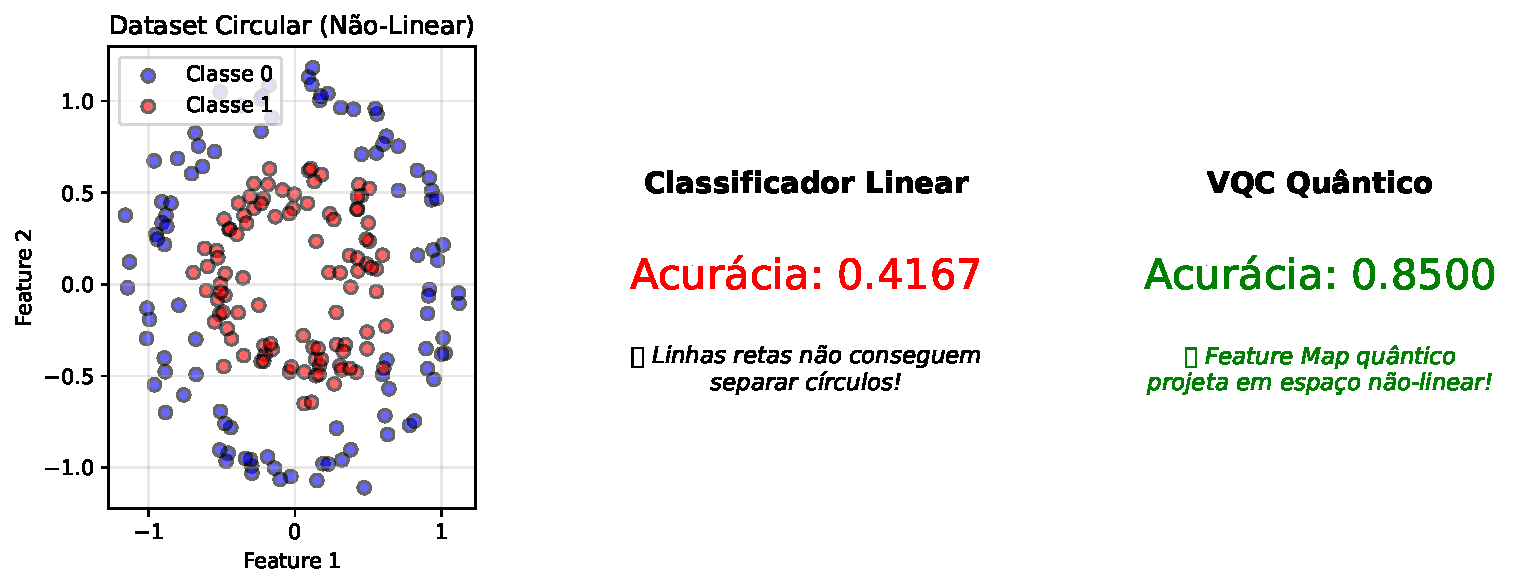
\includegraphics[keepaspectratio]{apostila_files/figure-pdf/cell-158-output-3.pdf}}

\begin{verbatim}

============================================================
COMPARAÇÃO EM DADOS NÃO-LINEARES (CÍRCULOS)
============================================================
Regressão Logística (Linear): 0.4167
VQC Quântico (Não-Linear):    0.8500
============================================================
\end{verbatim}

\begin{verbatim}
C:\Users\Max\AppData\Local\Temp\ipykernel_20596\3627597481.py:46: DeprecationWarning: The class ``qiskit.circuit.library.data_preparation._zz_feature_map.ZZFeatureMap`` is deprecated as of Qiskit 2.1. It will be removed in Qiskit 3.0. Use the zz_feature_map function as a replacement. Note that this will no longer return a BlueprintCircuit, but just a plain QuantumCircuit.
  feature_map=ZZFeatureMap(feature_dimension=2, reps=2),  # Aumentar reps para mais expressividade
C:\Users\Max\AppData\Local\Temp\ipykernel_20596\3627597481.py:47: DeprecationWarning: The class ``qiskit.circuit.library.n_local.real_amplitudes.RealAmplitudes`` is deprecated as of Qiskit 2.1. It will be removed in Qiskit 3.0. Use the function qiskit.circuit.library.real_amplitudes instead.
  ansatz=RealAmplitudes(num_qubits=2, reps=2),
No gradient function provided, creating a gradient function. If your Sampler requires transpilation, please provide a pass manager.
\end{verbatim}

\begin{verbatim}
Treinando VQC em dados circulares...
\end{verbatim}

\begin{verbatim}
C:\Users\Max\AppData\Local\Temp\ipykernel_20596\3627597481.py:63: UserWarning: Glyph 10060 (\N{CROSS MARK}) missing from font(s) DejaVu Sans.
  plt.subplots_adjust(wspace=0.4)
C:\Users\Max\AppData\Local\Temp\ipykernel_20596\3627597481.py:63: UserWarning: Glyph 9989 (\N{WHITE HEAVY CHECK MARK}) missing from font(s) DejaVu Sans.
  plt.subplots_adjust(wspace=0.4)
e:\temp\quantum\.venv\Lib\site-packages\IPython\core\pylabtools.py:170: UserWarning: Glyph 10060 (\N{CROSS MARK}) missing from font(s) DejaVu Sans.
  fig.canvas.print_figure(bytes_io, **kw)
e:\temp\quantum\.venv\Lib\site-packages\IPython\core\pylabtools.py:170: UserWarning: Glyph 9989 (\N{WHITE HEAVY CHECK MARK}) missing from font(s) DejaVu Sans.
  fig.canvas.print_figure(bytes_io, **kw)
\end{verbatim}

\begin{verbatim}

============================================================
COMPARAÇÃO EM DADOS NÃO-LINEARES (CÍRCULOS)
============================================================
Regressão Logística (Linear): 0.4167
VQC Quântico (Não-Linear):    0.8500
============================================================
\end{verbatim}

\begin{Shaded}
\begin{Highlighting}[]
\CommentTok{\# Visualizar as fronteiras de decisão}
\NormalTok{fig, axes }\OperatorTok{=}\NormalTok{ plt.subplots(}\DecValTok{1}\NormalTok{, }\DecValTok{2}\NormalTok{, figsize}\OperatorTok{=}\NormalTok{(}\DecValTok{14}\NormalTok{, }\DecValTok{5}\NormalTok{))}

\CommentTok{\# Fronteira Linear}
\NormalTok{h }\OperatorTok{=} \FloatTok{0.02}
\NormalTok{x\_min, x\_max }\OperatorTok{=}\NormalTok{ X\_circles\_norm[:, }\DecValTok{0}\NormalTok{].}\BuiltInTok{min}\NormalTok{() }\OperatorTok{{-}} \FloatTok{0.1}\NormalTok{, X\_circles\_norm[:, }\DecValTok{0}\NormalTok{].}\BuiltInTok{max}\NormalTok{() }\OperatorTok{+} \FloatTok{0.1}
\NormalTok{y\_min, y\_max }\OperatorTok{=}\NormalTok{ X\_circles\_norm[:, }\DecValTok{1}\NormalTok{].}\BuiltInTok{min}\NormalTok{() }\OperatorTok{{-}} \FloatTok{0.1}\NormalTok{, X\_circles\_norm[:, }\DecValTok{1}\NormalTok{].}\BuiltInTok{max}\NormalTok{() }\OperatorTok{+} \FloatTok{0.1}
\NormalTok{xx, yy }\OperatorTok{=}\NormalTok{ np.meshgrid(np.arange(x\_min, x\_max, h), np.arange(y\_min, y\_max, h))}

\CommentTok{\# Linear}
\NormalTok{Z\_lr }\OperatorTok{=}\NormalTok{ lr.predict(np.c\_[xx.ravel(), yy.ravel()])}
\NormalTok{Z\_lr }\OperatorTok{=}\NormalTok{ Z\_lr.reshape(xx.shape)}

\NormalTok{axes[}\DecValTok{0}\NormalTok{].contourf(xx, yy, Z\_lr, alpha}\OperatorTok{=}\FloatTok{0.4}\NormalTok{, cmap}\OperatorTok{=}\StringTok{\textquotesingle{}RdBu\textquotesingle{}}\NormalTok{, levels}\OperatorTok{=}\DecValTok{1}\NormalTok{)}
\NormalTok{axes[}\DecValTok{0}\NormalTok{].scatter(X\_circles\_norm[y\_circles }\OperatorTok{==} \DecValTok{0}\NormalTok{, }\DecValTok{0}\NormalTok{], X\_circles\_norm[y\_circles }\OperatorTok{==} \DecValTok{0}\NormalTok{, }\DecValTok{1}\NormalTok{], }
\NormalTok{               c}\OperatorTok{=}\StringTok{\textquotesingle{}blue\textquotesingle{}}\NormalTok{, label}\OperatorTok{=}\StringTok{\textquotesingle{}Classe 0\textquotesingle{}}\NormalTok{, edgecolors}\OperatorTok{=}\StringTok{\textquotesingle{}k\textquotesingle{}}\NormalTok{, s}\OperatorTok{=}\DecValTok{50}\NormalTok{, alpha}\OperatorTok{=}\FloatTok{0.7}\NormalTok{)}
\NormalTok{axes[}\DecValTok{0}\NormalTok{].scatter(X\_circles\_norm[y\_circles }\OperatorTok{==} \DecValTok{1}\NormalTok{, }\DecValTok{0}\NormalTok{], X\_circles\_norm[y\_circles }\OperatorTok{==} \DecValTok{1}\NormalTok{, }\DecValTok{1}\NormalTok{], }
\NormalTok{               c}\OperatorTok{=}\StringTok{\textquotesingle{}red\textquotesingle{}}\NormalTok{, label}\OperatorTok{=}\StringTok{\textquotesingle{}Classe 1\textquotesingle{}}\NormalTok{, edgecolors}\OperatorTok{=}\StringTok{\textquotesingle{}k\textquotesingle{}}\NormalTok{, s}\OperatorTok{=}\DecValTok{50}\NormalTok{, alpha}\OperatorTok{=}\FloatTok{0.7}\NormalTok{)}
\NormalTok{axes[}\DecValTok{0}\NormalTok{].set\_xlabel(}\StringTok{\textquotesingle{}Feature 1\textquotesingle{}}\NormalTok{)}
\NormalTok{axes[}\DecValTok{0}\NormalTok{].set\_ylabel(}\StringTok{\textquotesingle{}Feature 2\textquotesingle{}}\NormalTok{)}
\NormalTok{axes[}\DecValTok{0}\NormalTok{].set\_title(}\SpecialStringTok{f\textquotesingle{}Regressão Logística Linear}\CharTok{\textbackslash{}n}\SpecialStringTok{Acurácia: }\SpecialCharTok{\{}\NormalTok{lr\_score}\SpecialCharTok{:.4f\}}\SpecialStringTok{\textquotesingle{}}\NormalTok{)}
\NormalTok{axes[}\DecValTok{0}\NormalTok{].legend()}
\NormalTok{axes[}\DecValTok{0}\NormalTok{].grid(}\VariableTok{True}\NormalTok{, alpha}\OperatorTok{=}\FloatTok{0.3}\NormalTok{)}

\CommentTok{\# VQC Quântico}
\BuiltInTok{print}\NormalTok{(}\StringTok{"Calculando fronteira de decisão do VQC..."}\NormalTok{)}
\NormalTok{Z\_vqc }\OperatorTok{=}\NormalTok{ vqc\_circles.predict(np.c\_[xx.ravel(), yy.ravel()])}
\NormalTok{Z\_vqc }\OperatorTok{=}\NormalTok{ Z\_vqc.reshape(xx.shape)}

\NormalTok{axes[}\DecValTok{1}\NormalTok{].contourf(xx, yy, Z\_vqc, alpha}\OperatorTok{=}\FloatTok{0.4}\NormalTok{, cmap}\OperatorTok{=}\StringTok{\textquotesingle{}RdBu\textquotesingle{}}\NormalTok{, levels}\OperatorTok{=}\DecValTok{1}\NormalTok{)}
\NormalTok{axes[}\DecValTok{1}\NormalTok{].scatter(X\_circles\_norm[y\_circles }\OperatorTok{==} \DecValTok{0}\NormalTok{, }\DecValTok{0}\NormalTok{], X\_circles\_norm[y\_circles }\OperatorTok{==} \DecValTok{0}\NormalTok{, }\DecValTok{1}\NormalTok{], }
\NormalTok{               c}\OperatorTok{=}\StringTok{\textquotesingle{}blue\textquotesingle{}}\NormalTok{, label}\OperatorTok{=}\StringTok{\textquotesingle{}Classe 0\textquotesingle{}}\NormalTok{, edgecolors}\OperatorTok{=}\StringTok{\textquotesingle{}k\textquotesingle{}}\NormalTok{, s}\OperatorTok{=}\DecValTok{50}\NormalTok{, alpha}\OperatorTok{=}\FloatTok{0.7}\NormalTok{)}
\NormalTok{axes[}\DecValTok{1}\NormalTok{].scatter(X\_circles\_norm[y\_circles }\OperatorTok{==} \DecValTok{1}\NormalTok{, }\DecValTok{0}\NormalTok{], X\_circles\_norm[y\_circles }\OperatorTok{==} \DecValTok{1}\NormalTok{, }\DecValTok{1}\NormalTok{], }
\NormalTok{               c}\OperatorTok{=}\StringTok{\textquotesingle{}red\textquotesingle{}}\NormalTok{, label}\OperatorTok{=}\StringTok{\textquotesingle{}Classe 1\textquotesingle{}}\NormalTok{, edgecolors}\OperatorTok{=}\StringTok{\textquotesingle{}k\textquotesingle{}}\NormalTok{, s}\OperatorTok{=}\DecValTok{50}\NormalTok{, alpha}\OperatorTok{=}\FloatTok{0.7}\NormalTok{)}
\NormalTok{axes[}\DecValTok{1}\NormalTok{].set\_xlabel(}\StringTok{\textquotesingle{}Feature 1\textquotesingle{}}\NormalTok{)}
\NormalTok{axes[}\DecValTok{1}\NormalTok{].set\_ylabel(}\StringTok{\textquotesingle{}Feature 2\textquotesingle{}}\NormalTok{)}
\NormalTok{axes[}\DecValTok{1}\NormalTok{].set\_title(}\SpecialStringTok{f\textquotesingle{}VQC Quântico}\CharTok{\textbackslash{}n}\SpecialStringTok{Acurácia: }\SpecialCharTok{\{}\NormalTok{vqc\_score}\SpecialCharTok{:.4f\}}\SpecialStringTok{\textquotesingle{}}\NormalTok{)}
\NormalTok{axes[}\DecValTok{1}\NormalTok{].legend()}
\NormalTok{axes[}\DecValTok{1}\NormalTok{].grid(}\VariableTok{True}\NormalTok{, alpha}\OperatorTok{=}\FloatTok{0.3}\NormalTok{)}

\NormalTok{plt.subplots\_adjust(wspace}\OperatorTok{=}\FloatTok{0.4}\NormalTok{)}
\NormalTok{plt.show()}

\BuiltInTok{print}\NormalTok{(}\StringTok{"}\CharTok{\textbackslash{}n}\StringTok{💡 Observe:"}\NormalTok{)}
\BuiltInTok{print}\NormalTok{(}\StringTok{"   • O classificador linear cria apenas uma linha reta (limitado!)"}\NormalTok{)}
\BuiltInTok{print}\NormalTok{(}\StringTok{"   • O VQC consegue criar uma fronteira curva e não{-}linear"}\NormalTok{)}
\BuiltInTok{print}\NormalTok{(}\StringTok{"   • Isso acontece porque o Feature Map projeta os dados em um espaço de alta dimensão"}\NormalTok{)}
\end{Highlighting}
\end{Shaded}

\begin{verbatim}
Calculando fronteira de decisão do VQC...
\end{verbatim}

\pandocbounded{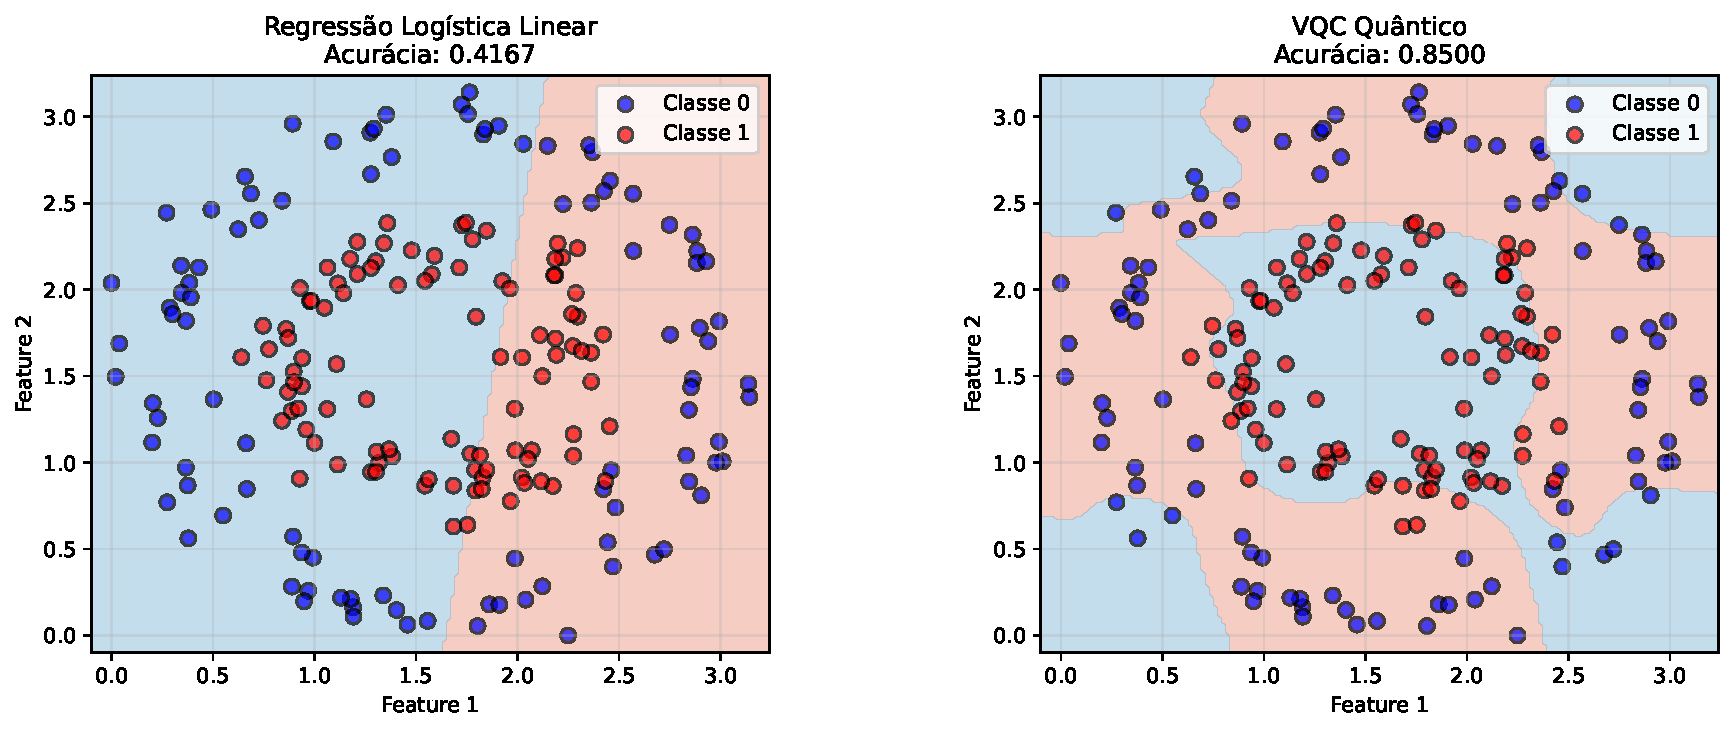
\includegraphics[keepaspectratio]{apostila_files/figure-pdf/cell-159-output-2.pdf}}

\begin{verbatim}

💡 Observe:
   • O classificador linear cria apenas uma linha reta (limitado!)
   • O VQC consegue criar uma fronteira curva e não-linear
   • Isso acontece porque o Feature Map projeta os dados em um espaço de alta dimensão
\end{verbatim}

\begin{verbatim}
Calculando fronteira de decisão do VQC...
\end{verbatim}

\begin{verbatim}

💡 Observe:
   • O classificador linear cria apenas uma linha reta (limitado!)
   • O VQC consegue criar uma fronteira curva e não-linear
   • Isso acontece porque o Feature Map projeta os dados em um espaço de alta dimensão
\end{verbatim}

\subsection{9. Resumo e Próximos
Passos}\label{resumo-e-pruxf3ximos-passos}

\subsubsection{🎓 O que aprendemos}\label{o-que-aprendemos}

Neste notebook, exploramos os fundamentos do \textbf{Quantum Machine
Learning (QML)} através de um \textbf{Classificador Variacional Quântico
(VQC)}:

\begin{enumerate}
\def\labelenumi{\arabic{enumi}.}
\tightlist
\item
  \textbf{Estrutura do VQC:}

  \begin{itemize}
  \tightlist
  \item
    \textbf{Feature Map:} Codifica dados clássicos em estados quânticos
  \item
    \textbf{Ansatz:} Circuito parametrizado que aprende (como pesos de
    uma rede neural)
  \item
    \textbf{Medição:} Extrai probabilidades de classificação
  \end{itemize}
\item
  \textbf{Conceitos Fundamentais:}

  \begin{itemize}
  \tightlist
  \item
    Espaço de Hilbert e projeção de alta dimensão
  \item
    Kernel trick quântico
  \item
    Otimização de parâmetros quânticos
  \end{itemize}
\item
  \textbf{Vantagens do QML:}

  \begin{itemize}
  \tightlist
  \item
    ✅ Capacidade de lidar com problemas não-lineares naturalmente
  \item
    ✅ Projeção em espaços de dimensão exponencial (2\^{}n)
  \item
    ✅ Potencial para superação quântica em problemas específicos
  \end{itemize}
\item
  \textbf{Limitações Atuais:}

  \begin{itemize}
  \tightlist
  \item
    ⚠️ Hardware quântico ainda limitado (poucos qubits, ruído)
  \item
    ⚠️ Treinamento pode ser lento
  \item
    ⚠️ Para muitos problemas, ML clássico ainda é superior
  \end{itemize}
\end{enumerate}

\subsubsection{🚀 Próximos Passos}\label{pruxf3ximos-passos-3}

Quer se aprofundar? Aqui estão sugestões de experimentos:

\textbf{Nível Iniciante:} 1. Mude o número de \texttt{reps} no Feature
Map e Ansatz - veja como afeta a acurácia 2. Teste diferentes
otimizadores: \texttt{SPSA}, \texttt{ADAM}, \texttt{L\_BFGS\_B} 3.
Experimente outros Feature Maps: \texttt{PauliFeatureMap},
\texttt{StatePreparation} 4. Altere o \texttt{maxiter} do otimizador

\textbf{Nível Intermediário:} 1. Use mais qubits (3 ou 4) e mais
features 2. Implemente um callback para visualizar o progresso do
treinamento 3. Compare com outros kernels do SVM: \texttt{poly},
\texttt{sigmoid} 4. Teste em datasets reais (Iris, Wine, etc.)

\textbf{Nível Avançado:} 1. Implemente um \textbf{Quantum Kernel}
customizado 2. Use um simulador com ruído (\texttt{FakeBackend}) 3.
Execute em hardware quântico real da IBM 4. Explore \textbf{Quantum
Neural Networks (QNN)} para regressão

\subsubsection{📖 Código para Copiar e
Experimentar}\label{cuxf3digo-para-copiar-e-experimentar}

\begin{Shaded}
\begin{Highlighting}[]
\CommentTok{\# Template para seus próprios experimentos}
\ImportTok{from}\NormalTok{ qiskit.circuit.library }\ImportTok{import}\NormalTok{ ZZFeatureMap, RealAmplitudes}
\ImportTok{from}\NormalTok{ qiskit\_algorithms.optimizers }\ImportTok{import}\NormalTok{ COBYLA}
\ImportTok{from}\NormalTok{ qiskit\_machine\_learning.algorithms }\ImportTok{import}\NormalTok{ VQC}

\CommentTok{\# Configure seu modelo aqui}
\NormalTok{my\_vqc }\OperatorTok{=}\NormalTok{ VQC(}
\NormalTok{    feature\_map}\OperatorTok{=}\NormalTok{ZZFeatureMap(feature\_dimension}\OperatorTok{=}\DecValTok{2}\NormalTok{, reps}\OperatorTok{=}\DecValTok{2}\NormalTok{),}
\NormalTok{    ansatz}\OperatorTok{=}\NormalTok{RealAmplitudes(num\_qubits}\OperatorTok{=}\DecValTok{2}\NormalTok{, reps}\OperatorTok{=}\DecValTok{3}\NormalTok{),  }\CommentTok{\# Experimente mudar!}
\NormalTok{    optimizer}\OperatorTok{=}\NormalTok{COBYLA(maxiter}\OperatorTok{=}\DecValTok{150}\NormalTok{),  }\CommentTok{\# Tente outros otimizadores}
\NormalTok{    loss}\OperatorTok{=}\StringTok{"cross\_entropy"}\NormalTok{,}
\NormalTok{)}

\CommentTok{\# Treine}
\NormalTok{my\_vqc.fit(X\_train, y\_train)}

\CommentTok{\# Avalie}
\BuiltInTok{print}\NormalTok{(}\SpecialStringTok{f"Acurácia: }\SpecialCharTok{\{}\NormalTok{my\_vqc}\SpecialCharTok{.}\NormalTok{score(X\_test, y\_test)}\SpecialCharTok{:.4f\}}\SpecialStringTok{"}\NormalTok{)}
\end{Highlighting}
\end{Shaded}

\subsubsection{🌟 Reflexão Final}\label{reflexuxe3o-final-1}

Quantum Machine Learning está na fronteira entre \textbf{computação
quântica} e \textbf{inteligência artificial}. Embora ainda não tenhamos
``vantagem quântica'' prática para a maioria dos problemas de ML,
estamos construindo as ferramentas e conhecimento que serão essenciais
quando computadores quânticos escaláveis estiverem disponíveis.

\textbf{A jornada está apenas começando!} 🚀

\subsubsection{🔗 Recursos Adicionais}\label{recursos-adicionais}

\begin{enumerate}
\def\labelenumi{\arabic{enumi}.}
\tightlist
\item
  Qiskit Documentation

  \begin{itemize}
  \tightlist
  \item
    https://qiskit.org/documentation
  \end{itemize}
\item
  Qiskit Machine Learning

  \begin{itemize}
  \tightlist
  \item
    https://qiskit.org/ecosystem/machine-learning
  \end{itemize}
\item
  Qiskit Textbook ⭐ (RECOMENDADO)

  \begin{itemize}
  \tightlist
  \item
    https://learn.qiskit.org
  \end{itemize}
\item
  PennyLane (Alternativa)

  \begin{itemize}
  \tightlist
  \item
    https://pennylane.ai
  \end{itemize}
\item
  Schuld \& Petruccione - ``Quantum Machine Learning''

  \begin{itemize}
  \tightlist
  \item
    \href{https://www.amazon.com/Machine-Learning-with-Quantum-Computers-_Quantum-Science-and-Technology_/dp/3030830977}{Amazon.com}
  \end{itemize}
\end{enumerate}

\newpage

\chapter{Módulo 14: Compilação Quântica e
Topologia}\label{muxf3dulo-14-compilauxe7uxe3o-quuxe2ntica-e-topologia}

\chapter{Aula 14 --- Compilação Quântica e Topologia do
Hardware}\label{aula-14-compilauxe7uxe3o-quuxe2ntica-e-topologia-do-hardware}

\chapter{Compilação quântica precisa respeitar a topologia do
hardware}\label{compilauxe7uxe3o-quuxe2ntica-precisa-respeitar-a-topologia-do-hardware}

Um circuito quântico descrito em uma linguagem de alto nível precisa ser
traduzido para as restrições físicas do dispositivo. A conectividade
entre qubits e o conjunto de portas disponíveis influenciam a forma como
o circuito pode ser executado.{[}{[}Quantum Computing - Vision and
Challenges{]}{]}

Portanto, o software quântico não é apenas uma camada abstrata
independente do hardware. A compilação é parte do desempenho do sistema
e precisa considerar a arquitetura física.

\section{Relações}\label{relauxe7uxf5es-1}

\begin{itemize}
\tightlist
\item
  {[}\hyperref[dispositivos-nisq-dependem-de-integrauxe7uxe3o-quuxe2ntico-cluxe1ssica]{Dispositivos
  NISQ dependem de integração quântico-clássica}{]}
\item
  {[}\hyperref[vantagem-quuxe2ntica-uxe9-dependente-da-classe-de-problemas]{Vantagem
  quântica é dependente da classe de problemas}{]}
\end{itemize}

\section{Fonte}\label{fonte-1}

\begin{itemize}
\tightlist
\item
  {[}1{]} https://arxiv.org/abs/2403.02240
\end{itemize}

\section{Prática com o Transpiler do
Qiskit}\label{pruxe1tica-com-o-transpiler-do-qiskit}

\begin{Shaded}
\begin{Highlighting}[]
\CommentTok{\# Compare o circuito lógico com o circuito transpilado para a topologia real do dispositivo}
\ImportTok{from}\NormalTok{ qiskit }\ImportTok{import}\NormalTok{ transpile}
\ImportTok{from}\NormalTok{ qiskit.providers.fake\_provider }\ImportTok{import}\NormalTok{ GenericBackendV2}

\CommentTok{\# qc\_logico = ... circuito da aula anterior}
\CommentTok{\# backend = GenericBackendV2(num\_qubits=5)}
\CommentTok{\# qc\_transpilado = transpile(qc\_logico, backend=backend, optimization\_level=3)}
\CommentTok{\# print(f"Portas antes: \{qc\_logico.size()\} | depois: \{qc\_transpilado.size()\}")}
\end{Highlighting}
\end{Shaded}

Observe como o transpiler insere portas SWAP para respeitar o grafo de
acoplamento físico, aumentando a profundidade do circuito.

\newpage

\chapter{Módulo 15: Impacto na Engenharia de
Software}\label{muxf3dulo-15-impacto-na-engenharia-de-software}

\chapter{Aula 15 --- Impacto na Engenharia de
Software}\label{aula-15-impacto-na-engenharia-de-software}

\section{Vantagem quântica é dependente da classe de
problemas}\label{vantagem-quuxe2ntica-uxe9-dependente-da-classe-de-problemas}

\chapter{Vantagem quântica é dependente da classe de
problemas}\label{vantagem-quuxe2ntica-uxe9-dependente-da-classe-de-problemas-1}

A computação quântica não oferece uma aceleração universal. A possível
vantagem depende da estrutura do problema, do algoritmo utilizado e da
capacidade de superar os custos de preparação, execução, medição e
pós-processamento.{[}{[}Quantum Computing - Vision and Challenges{]}{]}

Isso implica que a pergunta adequada não é se computadores quânticos são
simplesmente mais rápidos, mas quais classes de problemas podem se
beneficiar de suas propriedades físicas e algorítmicas.

\section{Relações}\label{relauxe7uxf5es-2}

\begin{itemize}
\tightlist
\item
  {[}\hyperref[dispositivos-nisq-dependem-de-integrauxe7uxe3o-quuxe2ntico-cluxe1ssica]{Dispositivos
  NISQ dependem de integração quântico-clássica}{]}
\item
  {[}\hyperref[compilauxe7uxe3o-quuxe2ntica-precisa-respeitar-a-topologia-do-hardware]{Compilação
  quântica precisa respeitar a topologia do hardware}{]}
\end{itemize}

\section{Fonte}\label{fonte-2}

\begin{itemize}
\tightlist
\item
  {[}1{]} https://arxiv.org/abs/2403.02240
\end{itemize}

\section{Tópicos para pesquisa
orientada}\label{tuxf3picos-para-pesquisa-orientada}

\begin{enumerate}
\def\labelenumi{\arabic{enumi}.}
\tightlist
\item
  Criptografia pós-quântica (NIST PQC): impacto de Shor sobre RSA/ECC e
  migração de algoritmos.
\item
  Teste e depuração de programas quânticos: como ``assertar''
  superposições?
\item
  Ciclo híbrido quântico-clássico (Qiskit Runtime primitives) e o papel
  do engenheiro de software.
\end{enumerate}




\end{document}
